% XeLaTeX starter: replace metadata and the body between BODY START / BODY END.
\documentclass[UTF8,12pt,a4paper,fontset=none]{ctexart}
\usepackage[a4paper,top=2.5cm,bottom=2.5cm,left=2.7cm,right=2.7cm,headheight=39pt,headsep=12pt]{geometry}
\usepackage{graphicx}
\usepackage{needspace,float,seqsplit}
\usepackage{longtable,booktabs,array,calc,tabularx}
\usepackage{enumitem}
\usepackage{amsmath,amssymb}
\usepackage{xcolor}
\usepackage{etoolbox}
\usepackage{hyperref}
\usepackage{fancyhdr,titlesec,tocloft,caption,url,indentfirst}
\usepackage[protrusion=false]{microtype}

% CONFIG START: all strings may be replaced for the current report.
\newcommand{\ReportType}{}
\newcommand{\ReportTitle}{系统分析与设计课程作业}
\newcommand{\ReportSubtitle}{安德鲁牙科系统设计文档}
\newcommand{\ReportCollege}{商学院}
\newcommand{\ReportClass}{信管2402}
\newcommand{\ReportStudentId}{1602242015}
\newcommand{\ReportAuthor}{张云福}
\newcommand{\ReportAdvisor}{毕文杰}
\newcommand{\ReportHeaderTitle}{安德鲁牙科系统设计}
\newif\ifShowFigureList
\ShowFigureListtrue
% CONFIG END

% Use regular static faces on Windows; VF files can resolve to ExtraLight/Thin.
\IfFileExists{C:/Windows/Fonts/simsun.ttc}{
  \setmainfont{SimSun}[BoldFont=SimHei]
  \setCJKmainfont{SimSun}[BoldFont=SimHei]
}{\IfFontExistsTF{Noto Serif CJK SC}{
  \setmainfont{Noto Serif CJK SC}\setCJKmainfont{Noto Serif CJK SC}
}{\IfFontExistsTF{Noto Serif SC}{
  \setmainfont{Noto Serif SC}[AutoFakeBold=2]\setCJKmainfont{Noto Serif SC}[AutoFakeBold=2]
}{\IfFontExistsTF{SimSun}{
  \setmainfont{SimSun}[BoldFont=SimHei]\setCJKmainfont{SimSun}[BoldFont=SimHei]
}{
  \setmainfont{FandolSong-Regular}[Extension=.otf,BoldFont=FandolSong-Bold]
  \setCJKmainfont{FandolSong-Regular}[Extension=.otf,BoldFont=FandolSong-Bold]
}}}}
\IfFileExists{C:/Windows/Fonts/Noto Sans SC Bold (TrueType).otf}{
  \setsansfont{Noto Sans SC (TrueType).otf}[Path=C:/Windows/Fonts/,BoldFont={Noto Sans SC Bold (TrueType).otf}]
  \setCJKsansfont{Noto Sans SC (TrueType).otf}[Path=C:/Windows/Fonts/,BoldFont={Noto Sans SC Bold (TrueType).otf}]
}{\IfFontExistsTF{Noto Sans CJK SC}{
  \setsansfont{Noto Sans CJK SC}\setCJKsansfont{Noto Sans CJK SC}
}{\IfFontExistsTF{Noto Sans SC}{
  \setsansfont{Noto Sans SC}\setCJKsansfont{Noto Sans SC}
}{\IfFontExistsTF{SimHei}{
  \setsansfont{SimHei}\setCJKsansfont{SimHei}
}{
  \setsansfont{FandolHei-Regular}[Extension=.otf,BoldFont=FandolHei-Bold]
  \setCJKsansfont{FandolHei-Regular}[Extension=.otf,BoldFont=FandolHei-Bold]
}}}}

% Compatibility verified for LaTeX 2025-11 + longtable 2025-10-13 v4.24.
% Limit this repair to that package date; later releases keep their own output.
\makeatletter
\IfFormatAtLeastTF{2025-11-01}{
  \@ifpackagelater{longtable}{2025/10/13}{
    \@ifpackagelater{longtable}{2025/10/14}{}{
      \patchcmd{\LT@output}{\vss}{\vfil}{}{\PackageWarning{csureport}{Inspect longtable compatibility}}
      \patchcmd{\LT@output}{\vss}{\vfil}{}{\PackageWarning{csureport}{Inspect longtable compatibility}}
    }
  }{}
}{}
\makeatother

\hypersetup{colorlinks=false,hidelinks,pdfauthor={\ReportAuthor},pdftitle={\ReportTitle},bookmarksnumbered=true}
\urlstyle{same}
\setlength{\parindent}{2em}
\setlength{\parskip}{0pt}
% Preserve ctexart's reference spacing: nominal 20pt becomes 26pt at 1.3.
\linespread{1.3}
\setlist{nosep,leftmargin=2em}
\titleformat{\section}{\bfseries\sffamily\fontsize{15pt}{20pt}\selectfont}{\thesection.}{0.6em}{}
\titleformat{\subsection}{\bfseries\sffamily\fontsize{14pt}{20pt}\selectfont}{\thesubsection}{0.6em}{}
\titleformat{\subsubsection}{\bfseries\sffamily\fontsize{12pt}{20pt}\selectfont}{\thesubsubsection}{0.6em}{}
\titlespacing*{\section}{0pt}{18pt}{8pt}
\titlespacing*{\subsection}{0pt}{14pt}{6pt}
\titlespacing*{\subsubsection}{0pt}{10pt}{4pt}
% Reserve space before hyperref places heading anchors at a page boundary.
\newcommand{\ReportHeadingSpace}[1]{\par\Needspace{#1\baselineskip}}
\pretocmd{\section}{\ReportHeadingSpace{4}}{}{\PackageWarning{csureport}{Inspect section spacing}}
\pretocmd{\subsection}{\ReportHeadingSpace{3}}{}{\PackageWarning{csureport}{Inspect subsection spacing}}
\pretocmd{\subsubsection}{\ReportHeadingSpace{3}}{}{\PackageWarning{csureport}{Inspect subsubsection spacing}}
\pagestyle{fancy}
\fancyhf{}
\setlength{\headheight}{39pt}
\newsavebox{\ReportHeaderBox}
\newcommand{\ReportHeaderLine}[1]{\begingroup
  \sbox{\ReportHeaderBox}{#1}%
  \ifdim\wd\ReportHeaderBox>\linewidth
    \resizebox{\linewidth}{!}{\usebox{\ReportHeaderBox}}%
  \else\usebox{\ReportHeaderBox}\fi\endgroup}
\fancyhead[L]{
\includegraphics[height=0.95cm]{media/csu_seal.png}}
\fancyhead[C]{\parbox[c][1.0cm][c]{0.48\textwidth}{\centering\sffamily\small 中南大学报告\\[-0.15em]\footnotesize \ReportHeaderTitle}}
\fancyhead[R]{\parbox[c][1.0cm][c]{0.24\textwidth}{\raggedleft\sffamily\footnotesize \ReportHeaderLine{\ReportCollege}\\\ReportHeaderLine{\ReportAuthor\quad\ReportStudentId}}}
\fancyfoot[C]{第\thepage 页}
\renewcommand{\headrulewidth}{0.6pt}
\newcommand{\infoblank}[1]{\underline{\makebox[6.4cm][c]{#1}}}
% Four Chinese character positions; the colon is outside the label box.
\newcommand{\ReportCoverLabel}[1]{\makebox[4em][s]{#1}：}
\newcommand{\ReportCode}[1]{\mbox{#1}}
\captionsetup{font=small,labelfont=bf}
\renewcommand{\contentsname}{目\quad 录}
\renewcommand{\cftsecleader}{\cftdotfill{\cftdotsep}}
\renewcommand{\listfigurename}{图\quad 录}
\tocloftpagestyle{fancy}
\renewcommand{\figurename}{图}
\renewcommand{\tablename}{表}
\setcounter{tocdepth}{2}
\setcounter{secnumdepth}{3}
\sloppy
\setlength{\emergencystretch}{2em}\clubpenalty=10000\widowpenalty=10000\displaywidowpenalty=10000
\setlength{\LTpre}{6pt}\setlength{\LTpost}{6pt}
\newcommand{\Cell}[1]{\begin{minipage}[t]{\linewidth}\raggedright\strut #1\strut\end{minipage}}

\begin{document}
\fontsize{12pt}{20pt}\selectfont
\hypersetup{pageanchor=false}
\begin{titlepage}
\thispagestyle{empty}
\begin{center}
\vspace*{0.3cm}

\includegraphics[width=0.92\textwidth,trim=0 0 26bp 0,clip]{media/csu_logo_full.png}\\[1.2cm]
\if\relax\detokenize\expandafter{\ReportType}\relax\else
{\sffamily\bfseries\fontsize{20pt}{30pt}\selectfont \ReportType\par}
\vspace{1.6cm}
\fi
{\sffamily\bfseries\fontsize{21pt}{31pt}\selectfont \ReportTitle\par}
\if\relax\detokenize\expandafter{\ReportSubtitle}\relax\else
\vspace{0.9cm}
{\fontsize{16pt}{24pt}\selectfont \ReportSubtitle\par}
\fi
\vfill
\renewcommand{\arraystretch}{1.75}
\begin{tabular}{@{}>{\bfseries\sffamily}r@{\hspace{0.55cm}}c@{}}
\ReportCoverLabel{学\hfill 院} & \infoblank{\ReportCollege}\\
\ReportCoverLabel{班\hfill 级} & \infoblank{\ReportClass}\\
\ReportCoverLabel{学\hfill 号} & \infoblank{\ReportStudentId}\\
\ReportCoverLabel{姓\hfill 名} & \infoblank{\ReportAuthor}\\
\ReportCoverLabel{指\hfill 导\hfill 教\hfill 师} & \infoblank{\ReportAdvisor}\\
\end{tabular}
\vfill
{\sffamily\fontsize{12pt}{20pt}\selectfont CENTRAL SOUTH UNIVERSITY\par}
\end{center}
\end{titlepage}
\hypersetup{pageanchor=true}
\pagenumbering{Roman}
\tableofcontents
\clearpage
\ifShowFigureList
\listoffigures
\clearpage
\fi
\renewcommand{\listtablename}{表\quad 录}
{\linespread{1}\fontsize{12pt}{17pt}\selectfont\renewcommand{\cfttabfont}{\normalfont\fontsize{12pt}{17pt}\selectfont}\listoftables}\clearpage
\pagenumbering{arabic}


\begin{center}{\sffamily\bfseries\fontsize{18pt}{26pt}\selectfont 安德鲁牙科系统设计文档\par}\end{center}
\begin{center}{\sffamily\bfseries\large 摘\quad 要}\end{center}
\noindent\hspace*{2em}安德鲁牙科连锁在广东经营15家门诊，计划三年内将门诊数量翻一番。各门诊相对独立，总部依靠人工监督；患者通过电话预约，医生又需要根据技能需求跨店服务。规模扩大后，患者资料如何连续使用、治疗计价能否统一、取消率如何比较，以及每位医生创造了多少经营价值，成为需要共同解决的问题。\par
目标系统增加小程序自助预约，并让电话代约与线上入口使用相同的医生班次和门诊容量。患者主档逐项记录过敏，治疗计划经确认后进入实际执行，医生记录标准单位数量与适用价格，每次就诊形成一张可追溯的结算单。总部按医生跨店归集季度收入、医疗用品成本及运营费用，计算净利润，并按10\%提取激励基金。文档依次给出业务现状与改进蓝图、系统用例规约、内部分析模型、关系数据库及界面和服务设计，同时定义并发、异常、权限与验收条件，为预约小程序和员工后台开发提供一致的业务依据。\par
关键词：牙科连锁；业务用例；跨店预约；单位计价；季度业绩；激励基金\par
\Needspace{459pt}
\section*{术语与业务对象}
\phantomsection\addcontentsline{toc}{section}{术语与业务对象}
\par\noindent\begin{minipage}{\textwidth}
{\fontsize{10.5pt}{13.2pt}\selectfont\setlength{\tabcolsep}{0pt}\renewcommand{\arraystretch}{1.08}
\captionof{table}{主要术语}\label{tab5}
\begin{tabular}{@{}p{3.040cm}@{\hspace{0.16cm}}p{12.240cm}@{}}
\toprule
\bfseries \Cell{术语} & \bfseries \Cell{含义与边界}\\\midrule
\Cell{顾客、患者与代办人} & \Cell{顾客入口面向患者及获得授权的代办人；患者是接受治疗的人，账号持有人可以不同。}\\[1pt]
\Cell{门诊、店长与总部} & \Cell{门诊是服务发生地点；店长承担本店运营和复核；总部负责统一规则、跨店协调及经营核算。}\\[1pt]
\Cell{治疗意向、计划与执行} & \Cell{意向用于预约；计划是医生提出并经患者选择的安排；执行是本次已经实施的事实。}\\[1pt]
\Cell{标准单位} & \Cell{治疗项目约定的计量单位。数量与单位价格共同决定该治疗行金额，不能把不同单位混算。}\\[1pt]
\Cell{Invoice} & \Cell{一次就诊唯一的业务结算单；包含明细与合计。本设计的Invoice不等同于税务机关开具的法定发票。}\\[1pt]
\Cell{应收、收款与收入} & \Cell{应收是患者应付的服务费用；收款是实际成功资金交易；收入用于已确认服务的经营归属，三者分别记录。}\\[1pt]
\Cell{业务日与季度} & \Cell{业务日按门诊营业日期核对资金；季度按服务与费用的获准归属期间汇总医生业绩。}\\[1pt]
\Cell{激励基金} & \Cell{按全体医生季度净利润合计的正值提取10\%，经独立复核后按明确规则分配；与股东分红分开。}\\[1pt]
\bottomrule\end{tabular}
}\end{minipage}\par\vspace{6pt}
\Needspace{9\baselineskip}
\Needspace{9\baselineskip}
\section{组织现状与升级目标}
\Needspace{3\baselineskip}
\subsection{连锁规模与经营诉求}
Andrew Chen兼任首席执行官与首席牙医。公司已有15家门诊，扩张计划要求门诊数量在三年内翻倍。门店以相对独立的方式经营，总部的人工监督难以持续回答治疗标准是否一致、各店取消率是否异常、医生技能组合是否满足需求等问题。股权安排解释决策责任，却不能代替医生经营贡献的核算依据。[资料1]\par
电话预约需要明确患者、门诊、接诊牙医与具体时间。患者主档还需要收集必要联系资料和逐项过敏。患者与医生都可能跨门诊活动：同一患者会接受不同医生的治疗，同一医生也会因技能需求在不同门诊出诊。跨店服务需要资料保持连续；如果不同门诊的记录缺乏统一关联，患者历史和医生季度价值就难以完整核对。\par
标准化结算与季度业绩是需要建立的业务能力。每次就诊可能包含多项治疗，诊疗期间还可能增加项目；医生需要记录标准单位数量及对应价格，结算单必须逐项可核对。经营评价则需要区分收入、医疗用品成本和医生运营费用，避免只看收款额或单店汇总。\par
\Needspace{522pt}
\subsection{业务问题与目标改变}
\par\noindent\begin{minipage}{\textwidth}
{\fontsize{10.5pt}{13.2pt}\selectfont\setlength{\tabcolsep}{0pt}\renewcommand{\arraystretch}{1.08}
\captionof{table}{业务现状、信息需求与目标改变}\label{tab12}
\begin{tabular}{@{}p{4.840cm}@{\hspace{0.16cm}}p{6.340cm}@{\hspace{0.16cm}}p{3.940cm}@{}}
\toprule
\bfseries \Cell{业务起点或需求} & \bfseries \Cell{目标改变} & \bfseries \Cell{责任与验收}\\\midrule
\Cell{电话提出需求并协调就诊时间} & \Cell{新增自助查询与预约；电话、现场协助使用同一容量池} & \Cell{店长发布资源，前台处理例外；同一时段不能重复承诺。}\\[1pt]
\Cell{医生与患者均可跨店，技能需求影响出诊} & \Cell{以统一身份组织资格、跨店班次及必要的临床交接} & \Cell{总部统一目录，店长协作排班；资格和全局冲突检查通过才能确认。}\\[1pt]
\Cell{到诊布尔值不能解释所有未出席原因} & \Cell{分别记录取消、改期、待到和确认未到，保留真实到诊时间} & \Cell{前台核实结果；取消率与未到率使用可下钻的分子分母。}\\[1pt]
\Cell{一次就诊多项治疗，治疗中可能增项} & \Cell{计划确认、实际执行、单位价格和结算明细连续关联} & \Cell{医生负责执行事实，患者确认增项，前台核对费用。}\\[1pt]
\Cell{需要一就诊一Invoice的标准化开单} & \Cell{唯一结算单身份加明细快照，费用调整和收退款保留原迹} & \Cell{相同就诊重复开单返回同一身份，不产生第二张有效单。}\\[1pt]
\Cell{总部人工监督，需掌握医生季度价值} & \Cell{医生跨店汇总收入、用品成本、运营费用和净利润} & \Cell{总部制表与复核分开；季度结果能还原到来源。}\\[1pt]
\Cell{净利润10\%构成激励基金} & \Cell{固定提取比例，补充亏损处理、个人权重及尾差分配规则} & \Cell{基金提取和个人分配可复算，发放不超批准额度。}\\[1pt]
\bottomrule\end{tabular}
}\end{minipage}\par\vspace{6pt}
\Needspace{435pt}
\subsection{愿景与可测量目标}
让患者在连锁内获得可兑现的就诊安排和连续服务，让每项治疗、费用及医生季度贡献都有一致而可追溯的记录。新增门诊沿用同一组业务规则，总部能够比较差异，门店能够明确履责。\par
\par\noindent\begin{minipage}{\textwidth}
{\fontsize{10.5pt}{13.2pt}\selectfont\setlength{\tabcolsep}{0pt}\renewcommand{\arraystretch}{1.08}
\captionof{table}{愿景的验收口径}\label{tab15}
\begin{tabular}{@{}p{2.440cm}@{\hspace{0.16cm}}p{4.840cm}@{\hspace{0.16cm}}p{5.640cm}@{\hspace{0.16cm}}p{2.040cm}@{}}
\toprule
\bfseries \Cell{目标} & \bfseries \Cell{评价对象} & \bfseries \Cell{目标条件} & \bfseries \Cell{责任岗位}\\\midrule
\Cell{目标业务覆盖} & \Cell{患者主档、有效预约、治疗执行、结算单和季度医生业绩可相互追溯} & \Cell{验收样本中必要关联完整率100\%；零跨患者引用} & \Cell{总部运营/\allowbreak{}财务}\\[1pt]
\Cell{预约一致性} & \Cell{两个入口竞争同一医生及牙椅时段} & \Cell{并发验收中最多一笔正式预约成功；失败方得到可恢复提示} & \Cell{店长/\allowbreak{}前台}\\[1pt]
\Cell{取消与未到可解释} & \Cell{按门诊、医生、期间汇总已结束且结果明确的预约} & \Cell{取消和未到分别列示；分子及分母可下钻，不预设降低百分比} & \Cell{总部运营}\\[1pt]
\Cell{技能匹配} & \Cell{发布班次和确认预约时核对有效资格} & \Cell{不允许资格不足或有效期不覆盖服务时间的预约} & \Cell{总部/\allowbreak{}店长}\\[1pt]
\Cell{季度核算可复算} & \Cell{医生收入、用品成本及运营费用形成季度明细} & \Cell{抽取任一医生可从结果还原来源；分摊和基金分配尾差为0分} & \Cell{总部财务}\\[1pt]
\Cell{跨店服务连续} & \Cell{同一患者及医生跨门诊使用统一身份} & \Cell{获授权人员能按一次就诊定位历史与交接，越权请求被拒绝} & \Cell{医生/\allowbreak{}总部}\\[1pt]
\bottomrule\end{tabular}
}\end{minipage}\par\vspace{6pt}
这些数值是设计验收目标，不是经营成效。取消率、候诊时长和填补率应在运行后建立基线，再比较相同口径、相同期间的结果；没有数据时不承诺降低比例。扩张容量按15家门诊到约30家的组织目标安排，不能据此推定实际患者量。\par
\Needspace{355pt}
\subsection{范围与岗位责任}
\par\noindent\begin{minipage}{\textwidth}
{\fontsize{10.5pt}{13.2pt}\selectfont\setlength{\tabcolsep}{0pt}\renewcommand{\arraystretch}{1.08}
\captionof{table}{五类登录角色及职责}\label{tab18}
\begin{tabular}{@{}p{2.140cm}@{\hspace{0.16cm}}p{6.840cm}@{\hspace{0.16cm}}p{6.140cm}@{}}
\toprule
\bfseries \Cell{角色} & \bfseries \Cell{主要职责} & \bfseries \Cell{关键边界}\\\midrule
\Cell{顾客} & \Cell{维护就诊人资料，查询与确认预约，确认方案，核对费用及查看本人的付款和复诊安排} & \Cell{不能凭家庭共用手机号查看他人病历；代办关系需核验。}\\[1pt]
\Cell{前台} & \Cell{电话代约、到诊接待、费用核对、收款、日结草稿及跟进待办} & \Cell{不能诊断、签署医生记录或批准自己提交的退款。}\\[1pt]
\Cell{医生} & \Cell{维护个人资格资料，检查诊断、拟定方案、确认执行、记录用品及签署病历} & \Cell{不能为提高业绩将未做治疗记为完成，也不能自行改动已关闭季度。}\\[1pt]
\Cell{店长} & \Cell{维护本店容量，协调跨店班次，核对门诊成本及日结，复核获授权的运营例外} & \Cell{运营权限不等于医生签署权；不得复核本人提交的受控事项。}\\[1pt]
\Cell{总部} & \Cell{统一门诊和目录，审核跨店规则，归集医生季度业绩，复核激励及管理权限} & \Cell{财务制表、复核、发放登记使用不同任务授权；默认不获得全部临床详情。}\\[1pt]
\bottomrule\end{tabular}
}\end{minipage}\par\vspace{6pt}
系统覆盖预约、患者资料、诊疗及结算、成本归属、期间复核与季度激励。线上支付和通知渠道作为辅助服务，通过经过核验的结果参与流程。库存采购、独立药房、技工生产、器械消毒和工资代发不展开为管理子系统；医疗用品成本通过治疗耗用和成本凭据归集。需要专业人员完成的医疗判断仍由医生承担。\par
\Needspace{9\baselineskip}
\Needspace{9\baselineskip}
\section{需求获取与行业调研}
\Needspace{3\baselineskip}
\subsection{资料研究与需求判断}
需求首先来自经营决策者对标准、取消率、技能与医生价值的关注，以及患者预约、治疗和计价过程中必须保存的信息。公开产品资料用于比较成熟做法，再转化为适合连锁组织的规则。产品存在某项功能，只能说明一种可参考的处理方式，不能证明安德鲁已经采用，也不能证明它能直接带来相同收益。\par
\par\noindent\begin{minipage}{\textwidth}
{\fontsize{10.5pt}{13.2pt}\selectfont\setlength{\tabcolsep}{0pt}\renewcommand{\arraystretch}{1.08}
\captionof{table}{需求获取方法及适用性}\label{tab23}
\begin{tabular}{@{}p{2.840cm}@{\hspace{0.16cm}}p{5.840cm}@{\hspace{0.16cm}}p{6.440cm}@{}}
\toprule
\bfseries \Cell{方法} & \bfseries \Cell{能获得的信息} & \bfseries \Cell{限制与适用条件}\\\midrule
\Cell{组织资料研究} & \Cell{组织规模、业务关系、资料字段及明确的信息需求} & \Cell{用于识别业务起点和核心约束；资料未说明的处理细节不能补写成现状。}\\[1pt]
\Cell{竞争产品公开资料研究} & \Cell{线上预约、治疗计划、收退款及跨店对账的成熟处理方式} & \Cell{已查阅官方页面；只记录页面明确支持的事实，不等同后台试用。}\\[1pt]
\Cell{现场观察与岗位访谈} & \Cell{实际交接、例外及工作量，能够检验岗位利益冲突} & \Cell{需要可追溯记录及受访者确认，适合验证组织内部的例外处理。}\\[1pt]
\Cell{问卷} & \Cell{患者渠道偏好、提醒接受度等分布} & \Cell{样本代表性与题目设计会影响结论，不能替代具体业务规则核实。}\\[1pt]
\Cell{操作体验与原型走查} & \Cell{输入错误、状态理解及业务路径是否顺畅} & \Cell{适合检验交互与流程，但不能替代实际运行中的容量和经营效果验证。}\\[1pt]
\bottomrule\end{tabular}
}\end{minipage}\par\vspace{6pt}
\Needspace{9\baselineskip}
\Needspace{9\baselineskip}
\subsection{公开产品能力与设计取舍}
\Needspace{3\baselineskip}
\subsubsection{R1 Curve Dental：Multisite Success: Streamline Your Front Office}
公开资料说明：支持跨门诊切换日历和患者自助预约，可控制开放项目并发送复诊短信提醒，前台能接续诊疗信息。 设计取舍：线上预约、电话代约共用医生与门诊日历；仅向患者开放适合自助预约的服务。 没有据此认定其能够按安德鲁所需资格自动安排跨店班次。 [R1]\par
\subsubsection{R2 Dentally Help Centre：How to use waiting lists}
公开资料说明：候补记录注明门诊和预约原因，同时保留所需时长与等待状态，可辅助填补取消后的空档。 设计取舍：取消后先释放资源，再匹配候补并取得患者确认；邀请与预约分开。 公开说明不能证明候补会自动转成已确认预约。 [R2]\par
\subsubsection{R3 领健 e看牙帮助中心：【治疗计划】功能介绍}
公开资料说明：治疗计划联系诊断与牙位，并关联方案步骤、收费项目和同意文件，支持分步骤执行并区分预收和执行收入。 设计取舍：治疗意向、已确认计划、实际执行与当次结算分别记录；增项先确认再执行。 借鉴对象关系和交接方式，不将产品报表口径当成安德鲁已执行的财务制度。 [R3]\par
\subsubsection{R4 Open Dental：Payment}
公开资料说明：收款可以分配到欠费项目，并联系医生、门诊及未分配余额；分配合计需要与收款对应。 设计取舍：收款与应收分配分开保存，付款门诊和服务门诊分别记录，部分付款保留欠款。 不照搬境外保险、税务和具体界面操作。 [R4]\par
\subsubsection{R5 Open Dental：Refund}
公开资料说明：退款处理需要追溯原付款及款项分配，存在部分退款和不同退款原因。 设计取舍：费用调整与实际退钱分开，独立复核后退款，保留原始交易及调整关系。 退款权限及费用减免规则属于目标制度设计，不推定为机构既有做法。 [R5]\par
\subsubsection{R6 Dentrix Ascend Academy：Payment Location Cross-Reconciliation Report}
公开资料说明：跨地点核对报告区分服务与收款地点，为门诊间必要的资金划转提供依据。 设计取舍：总部按服务发生门诊和医生归集业绩；跨店代收单独核对，不再次形成营业收入。 报告功能不能证明其采用安德鲁的季度激励公式。 [R6]\par
\Needspace{378pt}
\subsubsection{R7 Dentally Help Centre：How appointment slots are held during online booking with Portal}
公开资料说明：线上选择时段后可以临时保留，确认后成为预约，未完成且到期时释放。 设计取舍：查询、短时占位、正式预约分开，最终确认时重新检查资格与资源。 保留期限由运营规则确定，不照搬厂商数值。 [R7]\par
\par\noindent\begin{minipage}{\textwidth}
{\fontsize{10.5pt}{13.2pt}\selectfont\setlength{\tabcolsep}{0pt}\renewcommand{\arraystretch}{1.08}
\captionof{table}{业务关注点与调研启示的联系}\label{tab39}
\begin{tabular}{@{}p{4.240cm}@{\hspace{0.16cm}}p{2.240cm}@{\hspace{0.16cm}}p{8.640cm}@{}}
\toprule
\bfseries \Cell{业务关注点} & \bfseries \Cell{可借鉴资料} & \bfseries \Cell{目标方案的具体改变}\\\midrule
\Cell{电话协调、跨店信息分散} & \Cell{R1、R7} & \Cell{统一日历与短时占位，线上自助和人工代约竞争相同资源。}\\[1pt]
\Cell{取消情况需要跟踪和解释} & \Cell{R2} & \Cell{取消记录原因并释放资源，候补先邀请后确认，同时单列未到。}\\[1pt]
\Cell{治疗增项需要追溯计价来源} & \Cell{R3} & \Cell{方案版本与同意相联系，执行保存单位价快照，账单来自执行行。}\\[1pt]
\Cell{费用、收款和退款需要分别核对} & \Cell{R4、R5} & \Cell{应收、实际成功交易、分配与费用调整分别建模，部分付款和在途状态可见。}\\[1pt]
\Cell{跨店服务与医生季度评价} & \Cell{R6} & \Cell{服务门诊、实际医生和收款门诊分别保存；总部在统一口径下汇总季度。}\\[1pt]
\bottomrule\end{tabular}
}\end{minipage}\par\vspace{6pt}
\Needspace{395pt}
\subsection{涉众利益与制度选择}
\par\noindent\begin{minipage}{\textwidth}
{\fontsize{10.5pt}{13.2pt}\selectfont\setlength{\tabcolsep}{0pt}\renewcommand{\arraystretch}{1.08}
\captionof{table}{主要利益平衡}\label{tab41}
\begin{tabular}{@{}p{4.240cm}@{\hspace{0.16cm}}p{6.040cm}@{\hspace{0.16cm}}p{4.840cm}@{}}
\toprule
\bfseries \Cell{冲突} & \bfseries \Cell{取舍} & \bfseries \Cell{约束与后果}\\\midrule
\Cell{患者希望立即确认，门诊需要检查复杂项目条件} & \Cell{标准服务允许即时确认；复杂治疗由医生确认适配后安排} & \Cell{申请状态与预约成功分开，等待人工处理必须有责任人。}\\[1pt]
\Cell{医生跨店提供服务，门店希望独占医生容量} & \Cell{资格、时间和转场作为全局约束，店长协作调整} & \Cell{任何一家门诊都不能单独绕过其他店已确认的安排。}\\[1pt]
\Cell{患者希望少填资料，临床需要完整风险信息} & \Cell{保留关键字段，过敏状态显式询问，线上预填到诊复核} & \Cell{邮箱可选；未核对资料保留状态，不能自动视为无过敏。}\\[1pt]
\Cell{及时结账与准确确认服务} & \Cell{前台只能对已签署实际执行生成费用} & \Cell{未做项目不计收入，治疗中增项先确认。}\\[1pt]
\Cell{激励促进贡献，核算需保留亏损与共同费用} & \Cell{先计算含负贡献的总净利润，再提取10\%；个人按正净贡献分配} & \Cell{分配方法和亏损不提取为明确制度选择；不按股权比例分配。}\\[1pt]
\Cell{总部可比性与医生、患者隐私} & \Cell{总部经营报表只含所需事实和来源标识} & \Cell{查询病历需另外授权，审计能够追到具体操作者。}\\[1pt]
\bottomrule\end{tabular}
}\end{minipage}\par\vspace{6pt}
\Needspace{9\baselineskip}
\Needspace{584pt}
\section{业务建模与改进蓝图}
\Needspace{3\baselineskip}
\subsection{组织对外提供的价值}
业务用例描述患者从组织获得的完整价值。前台、医生、店长与总部是完成服务的业务工人；患者是外部业务执行者。总部季度核算作为内部经营支撑，与患者服务产生的治疗和结算事实相联系。\par
\begin{figure}[H]\centering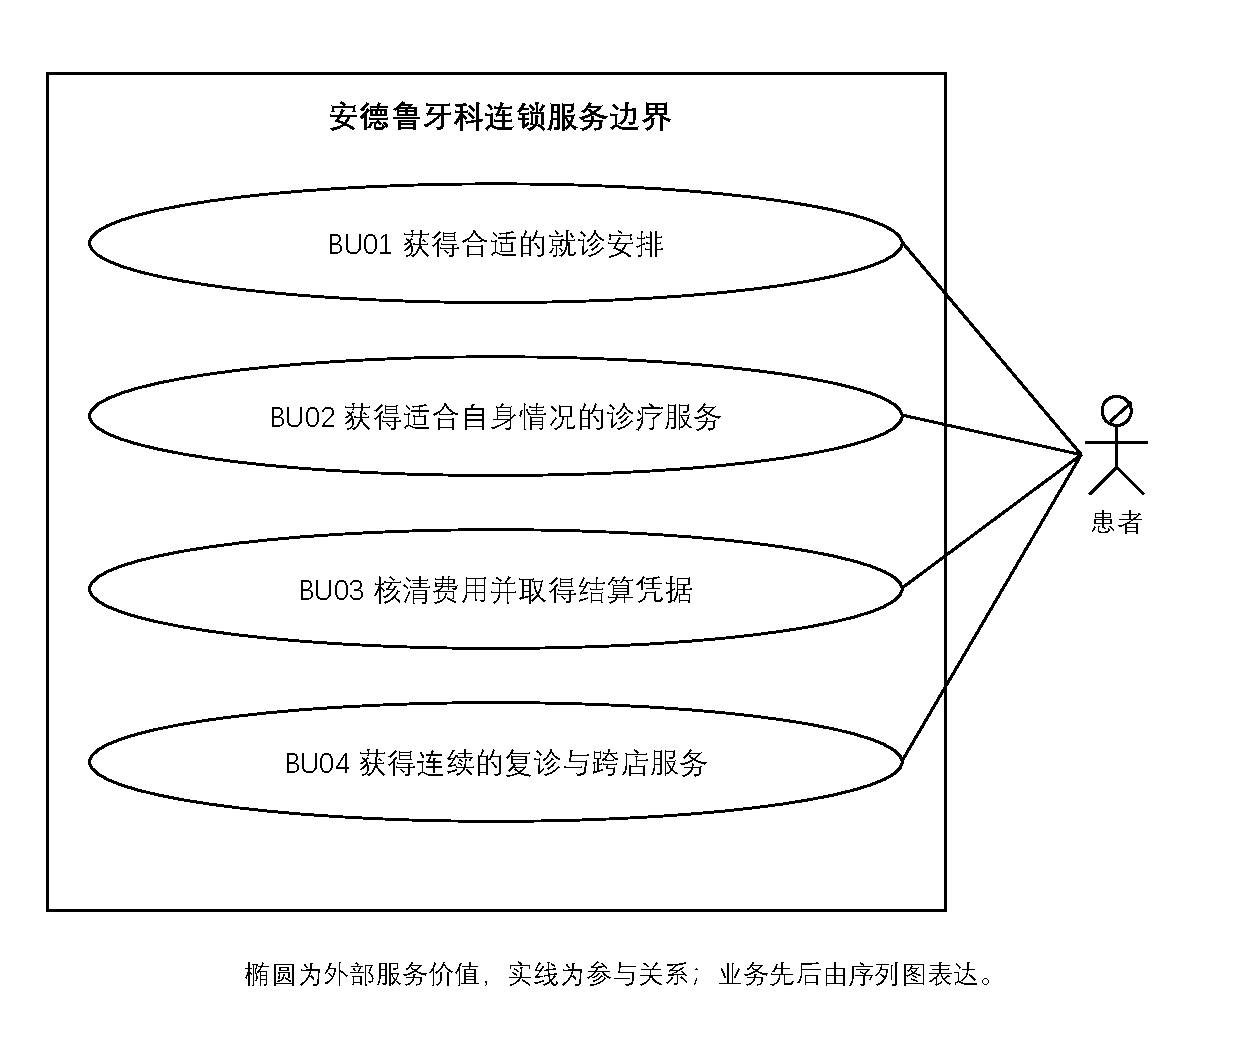
\includegraphics[width=\textwidth]{figures/business_overview.pdf}
\caption{患者服务业务用例}\label{business_overview}\end{figure}
\par\noindent\begin{minipage}{\textwidth}
{\fontsize{10.5pt}{13.2pt}\selectfont\setlength{\tabcolsep}{0pt}\renewcommand{\arraystretch}{1.08}
\captionof{table}{业务用例约定}\label{tab46}
\begin{tabular}{@{}p{3.340cm}@{\hspace{0.16cm}}p{4.840cm}@{\hspace{0.16cm}}p{4.440cm}@{\hspace{0.16cm}}p{2.340cm}@{}}
\toprule
\bfseries \Cell{编号与价值} & \bfseries \Cell{服务内容} & \bfseries \Cell{可观察的结束条件} & \bfseries \Cell{实现过程}\\\midrule
\Cell{\mbox{BU01} 获得合适的就诊安排} & \Cell{患者提出治疗意向和时间地点偏好，获得与医生资格和可用容量匹配的明确安排。} & \Cell{以已确认安排或明确未能安排及后续处理结束；浏览号源不算完成。} & \Cell{\mbox{BP01}、\mbox{BP02}、\mbox{BP03}}\\[1pt]
\Cell{\mbox{BU02} 获得适合自身情况的诊疗服务} & \Cell{患者提供健康及过敏资料，与医生确认方案，接受已同意的实际治疗。} & \Cell{形成签署诊疗记录、实际执行事实和后续安排；增项经过确认。} & \Cell{\mbox{BP04}、\mbox{BP05}}\\[1pt]
\Cell{\mbox{BU03} 核清费用并取得结算凭据} & \Cell{患者核对本次治疗明细，支付应付款项，并能追溯费用更正和退款。} & \Cell{同次就诊唯一结算单，付款或欠款状态明确，更正保留原始凭据。} & \Cell{\mbox{BP06}、\mbox{BP08}}\\[1pt]
\Cell{\mbox{BU04} 获得连续的复诊与跨店服务} & \Cell{患者在同一连锁内继续既定治疗，交接时保留必要历史、责任医生及阶段条件。} & \Cell{后续任务有接收责任人；复诊预约或跨店接收结果可查。} & \Cell{\mbox{BP07}}\\[1pt]
\bottomrule\end{tabular}
}\end{minipage}\par\vspace{6pt}
\subsection{现状业务序列}
患者先通过电话表达需求并约定医生和时间，到诊后由医生处理问题、特殊需求及实际治疗。下面两张现状序列图呈现这些业务工人与业务实体的交接；统一开单、取消原因分析和医生季度核算在目标蓝图中展开。\par
患者致电提出治疗需求，并约定接诊牙医、门诊和具体时间。就诊安排作为业务实体表达双方形成的服务约定。\par
\begin{figure}[H]\centering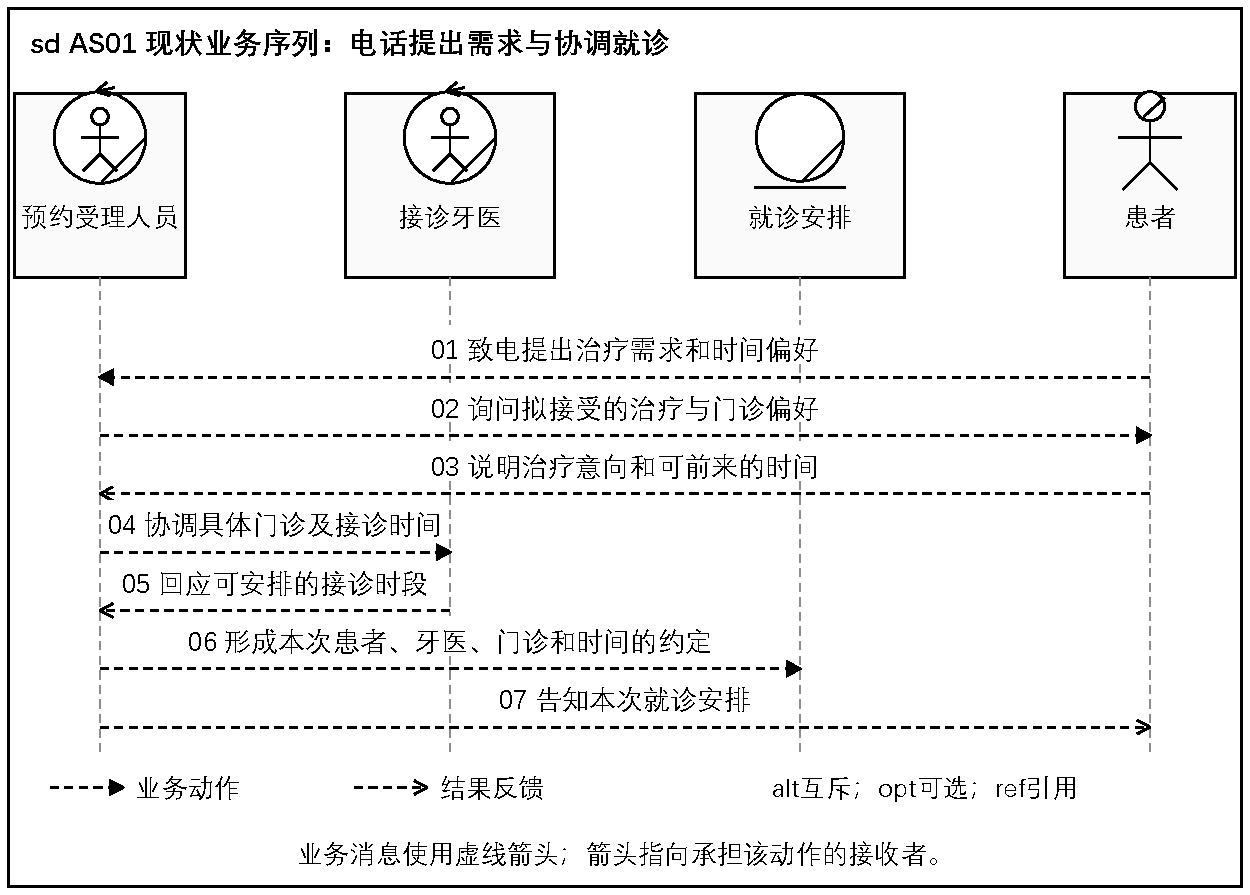
\includegraphics[width=\textwidth]{figures/AS01.pdf}
\caption{AS01 现状业务序列：电话提出需求与协调就诊}\label{AS01}\end{figure}
患者按具体日期时间前来，向牙医说明问题或特殊需求并接受治疗。标准单位记录、统一结算单和季度业绩属于进一步提出的信息要求，在目标蓝图中落实。\par
\begin{figure}[H]\centering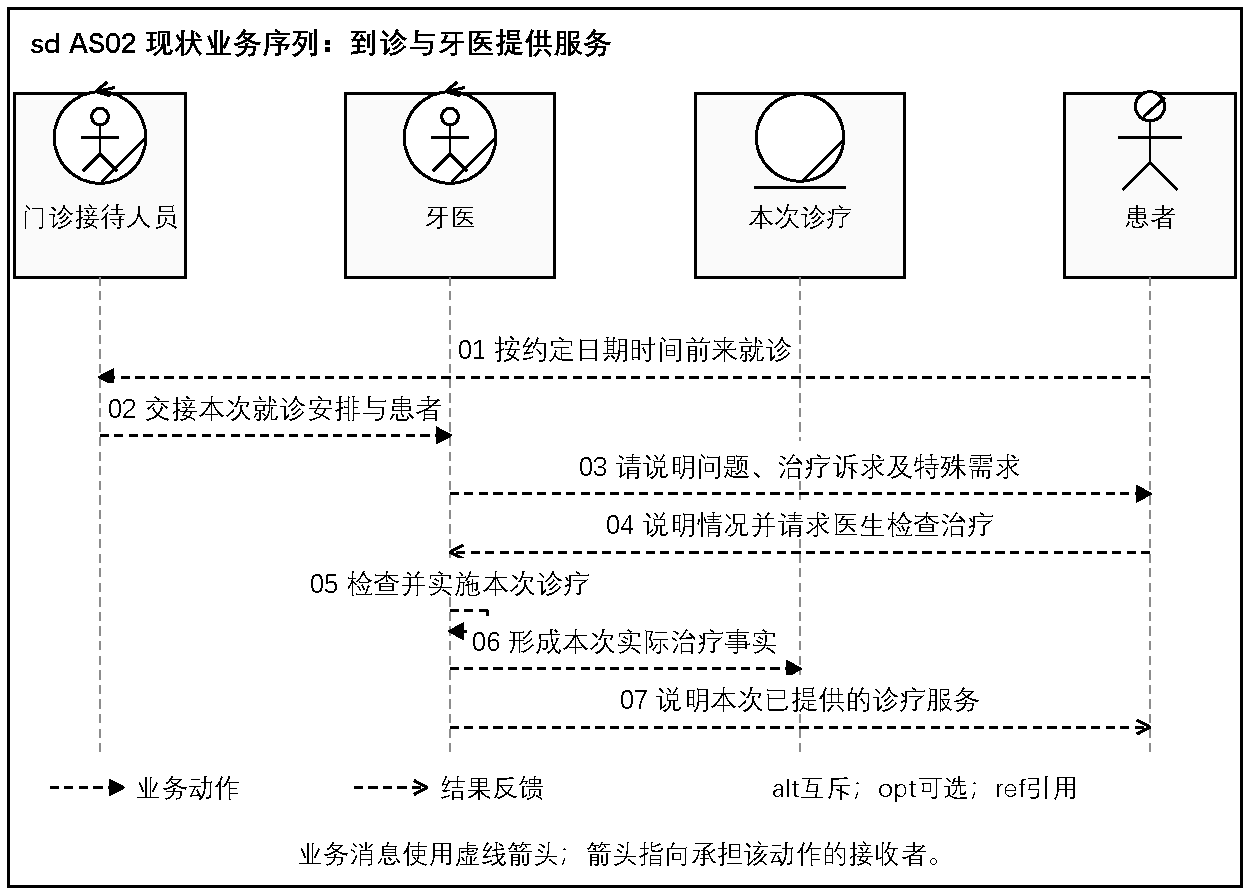
\includegraphics[width=\textwidth]{figures/AS02.pdf}
\caption{AS02 现状业务序列：到诊与牙医提供服务}\label{AS02}\end{figure}
\Needspace{442pt}
\subsection{患者服务的目标蓝图}
业务消息按自上而下的顺序阅读，虚线箭头指向负责处理该动作的接收者。业务工人与业务实体使用相应图标，外部患者放在右侧；平台只承担信息处理与规则校验。alt表示条件互斥，opt表示满足条件时才执行。分图保留参与者和原消息编号，下一图接续上一图。\par
\par\noindent\begin{minipage}{\textwidth}
{\fontsize{10.5pt}{13.2pt}\selectfont\setlength{\tabcolsep}{0pt}\renewcommand{\arraystretch}{1.08}
\captionof{table}{目标业务过程与系统用例}\label{tab55}
\begin{tabular}{@{}p{4.240cm}@{\hspace{0.16cm}}p{3.140cm}@{\hspace{0.16cm}}p{7.740cm}@{}}
\toprule
\bfseries \Cell{过程} & \bfseries \Cell{关联用例} & \bfseries \Cell{核心交接条件}\\\midrule
\Cell{\mbox{BP01} 医生资格及跨店排班} & \Cell{\mbox{UC-02}至\mbox{UC-04}} & \Cell{资格有效、时间不重叠才能发布容量。}\\[1pt]
\Cell{\mbox{BP02} 自助及前台代约} & \Cell{\mbox{UC-01}、\mbox{UC-05}、\mbox{UC-06}} & \Cell{共同资源池，最终确认与临时占位分开。}\\[1pt]
\Cell{\mbox{BP03} 改期取消与候补} & \Cell{\mbox{UC-07}、\mbox{UC-08}} & \Cell{变更失败保留旧约；候补接受后再竞争资源。}\\[1pt]
\Cell{\mbox{BP04} 到诊、检查及方案} & \Cell{\mbox{UC-09}至\mbox{UC-11}} & \Cell{核对实际到诊、过敏及方案确认。}\\[1pt]
\Cell{\mbox{BP05} 执行及记录} & \Cell{\mbox{UC-11}至\mbox{UC-13}} & \Cell{仅执行已同意范围，签署后通过附记更正。}\\[1pt]
\Cell{\mbox{BP06} 结算、收款与退款} & \Cell{\mbox{UC-15}至\mbox{UC-17}} & \Cell{一就诊一单，独立核验支付及退款。}\\[1pt]
\Cell{\mbox{BP07} 跨店诊疗交接} & \Cell{\mbox{UC-14}} & \Cell{患者授权且接收医生明确接受后开放预约。}\\[1pt]
\Cell{\mbox{BP08} 日结与代收} & \Cell{\mbox{UC-18}} & \Cell{总部核对先于日结正式通过，划转另核实。}\\[1pt]
\Cell{\mbox{BP09} 成本与期间} & \Cell{\mbox{UC-19}、\mbox{UC-20}} & \Cell{费用归属守恒，差异阻断关账。}\\[1pt]
\Cell{\mbox{BP10} 季度业绩与激励} & \Cell{\mbox{UC-21}、\mbox{UC-22}} & \Cell{完整来源后提取10\%，分配复核后登记发放。}\\[1pt]
\bottomrule\end{tabular}
}\end{minipage}\par\vspace{6pt}
\begin{figure}[H]\centering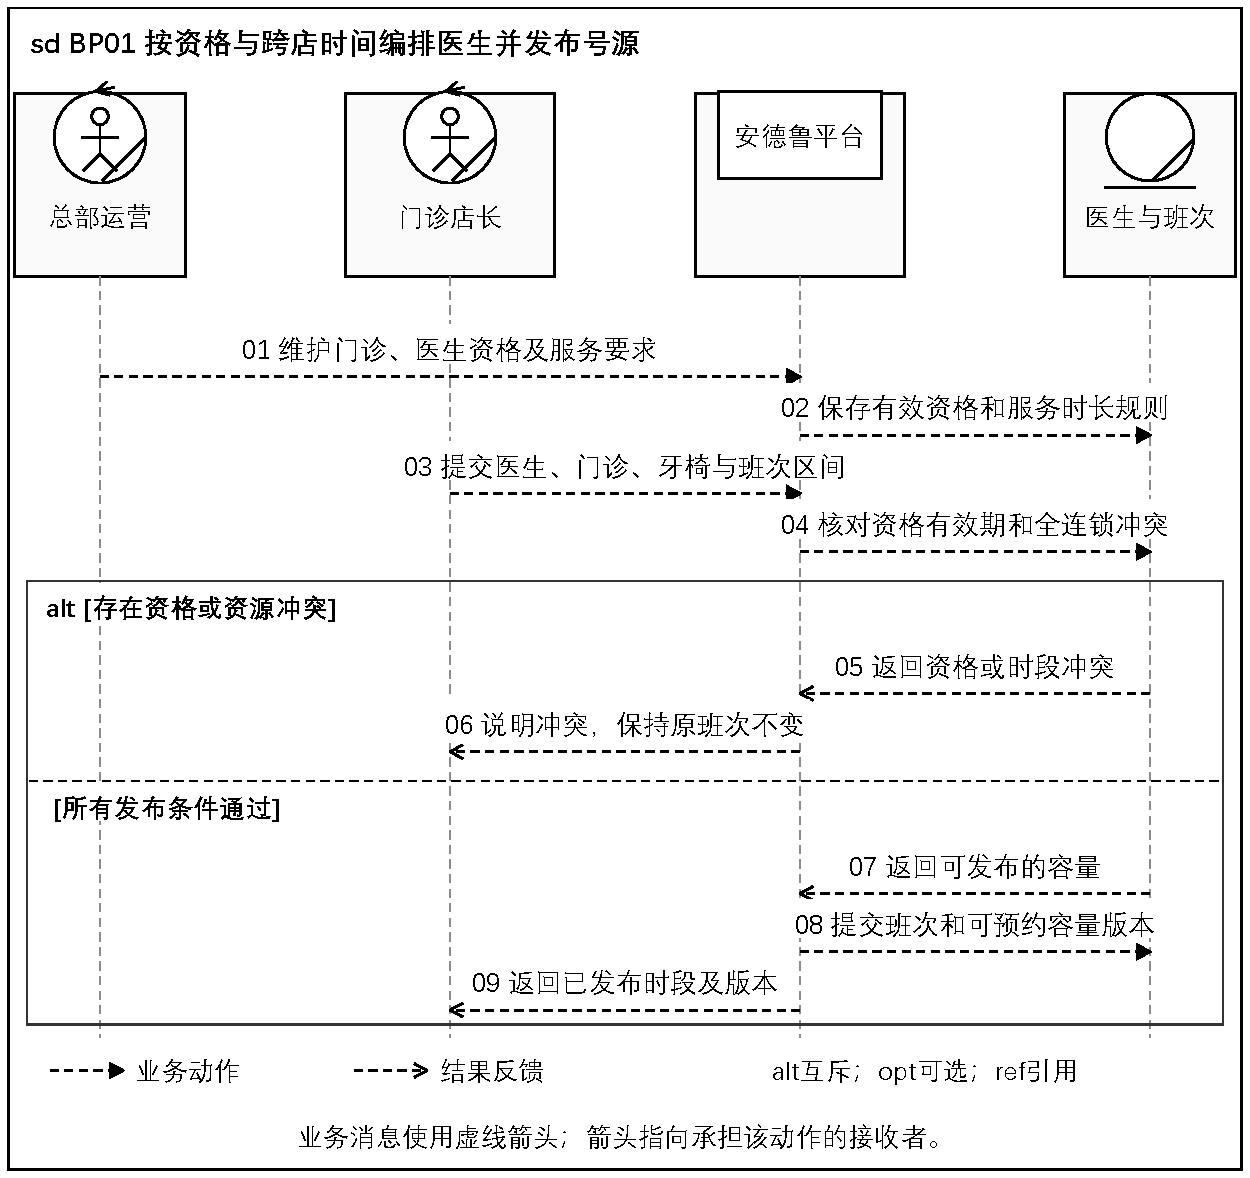
\includegraphics[width=\textwidth]{figures/BP01.pdf}
\caption{BP01 按资格与跨店时间编排医生并发布号源}\label{BP01}\end{figure}
\begin{figure}[H]\centering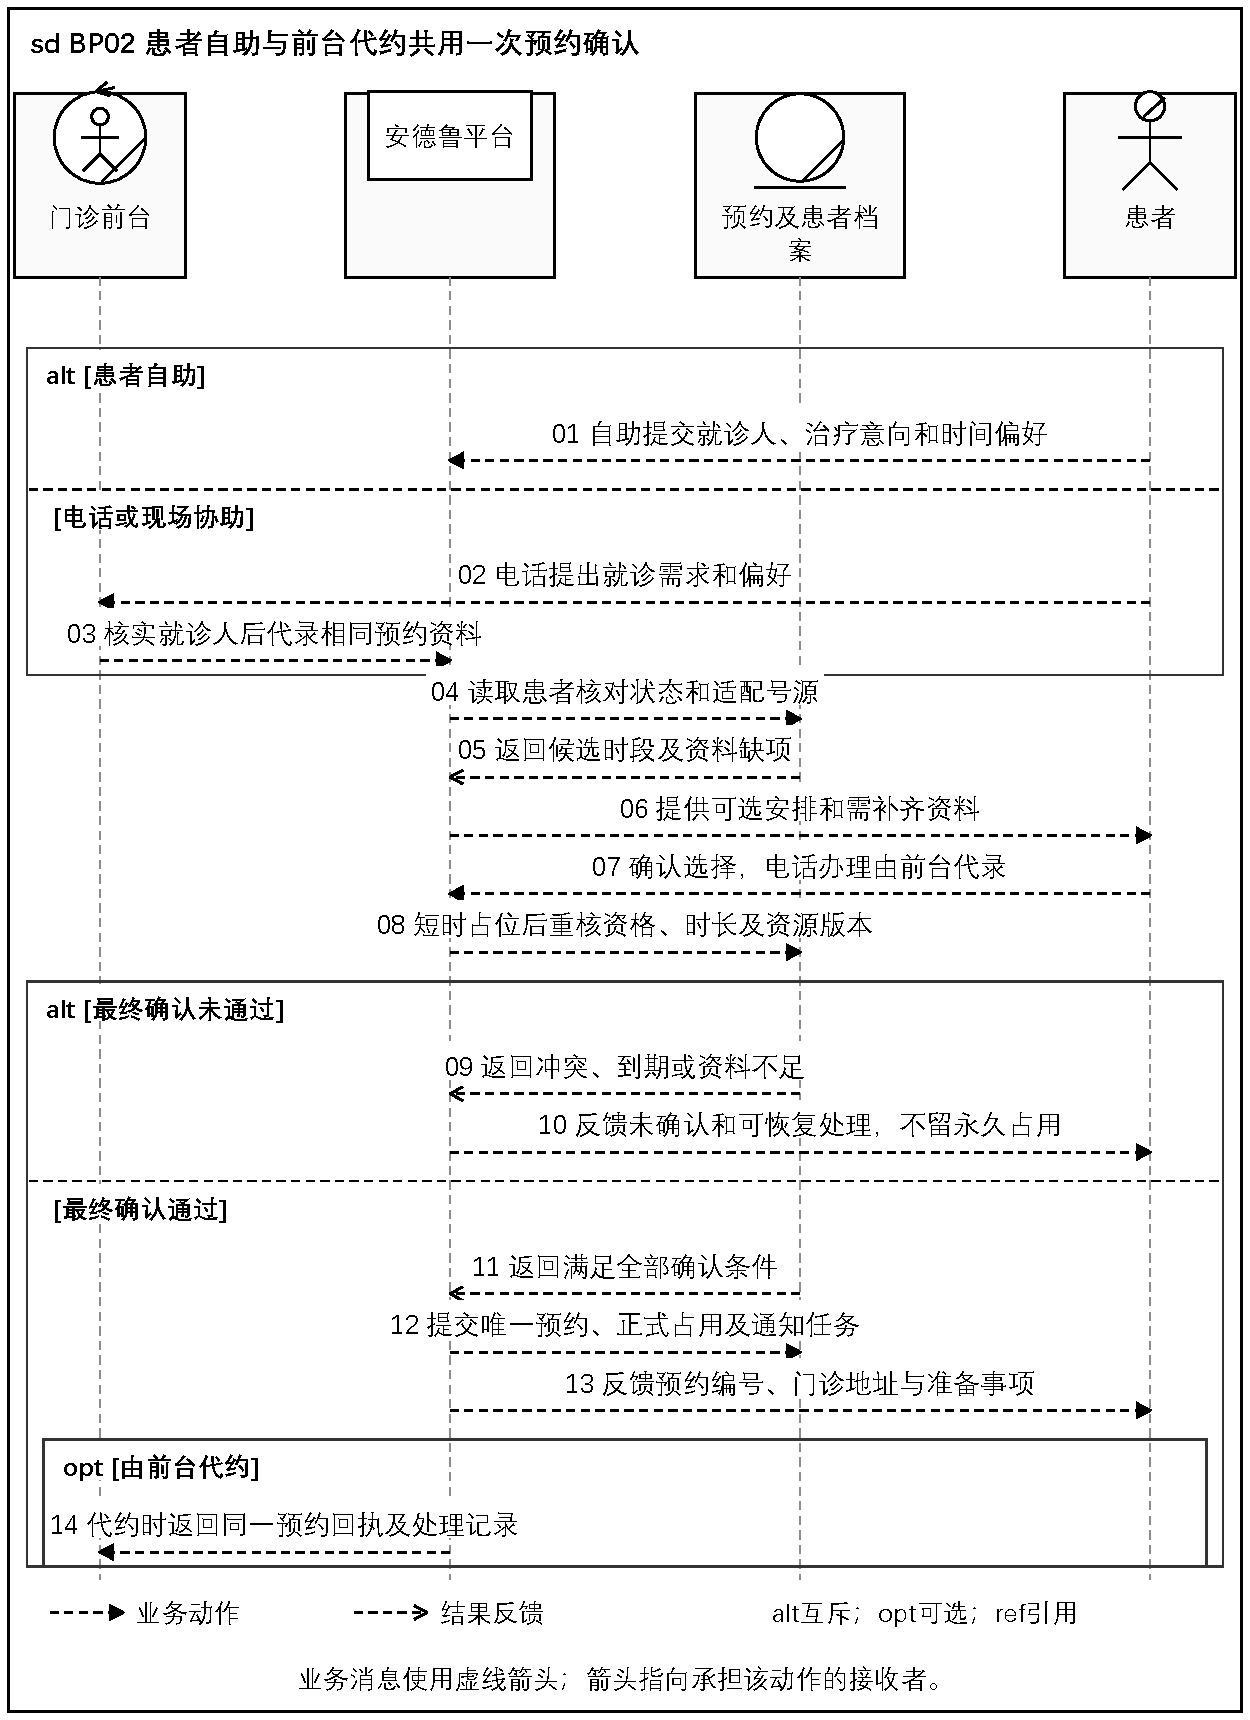
\includegraphics[width=\textwidth]{figures/BP02.pdf}
\caption{BP02 患者自助与前台代约共用一次预约确认}\label{BP02}\end{figure}
\begin{figure}[H]\centering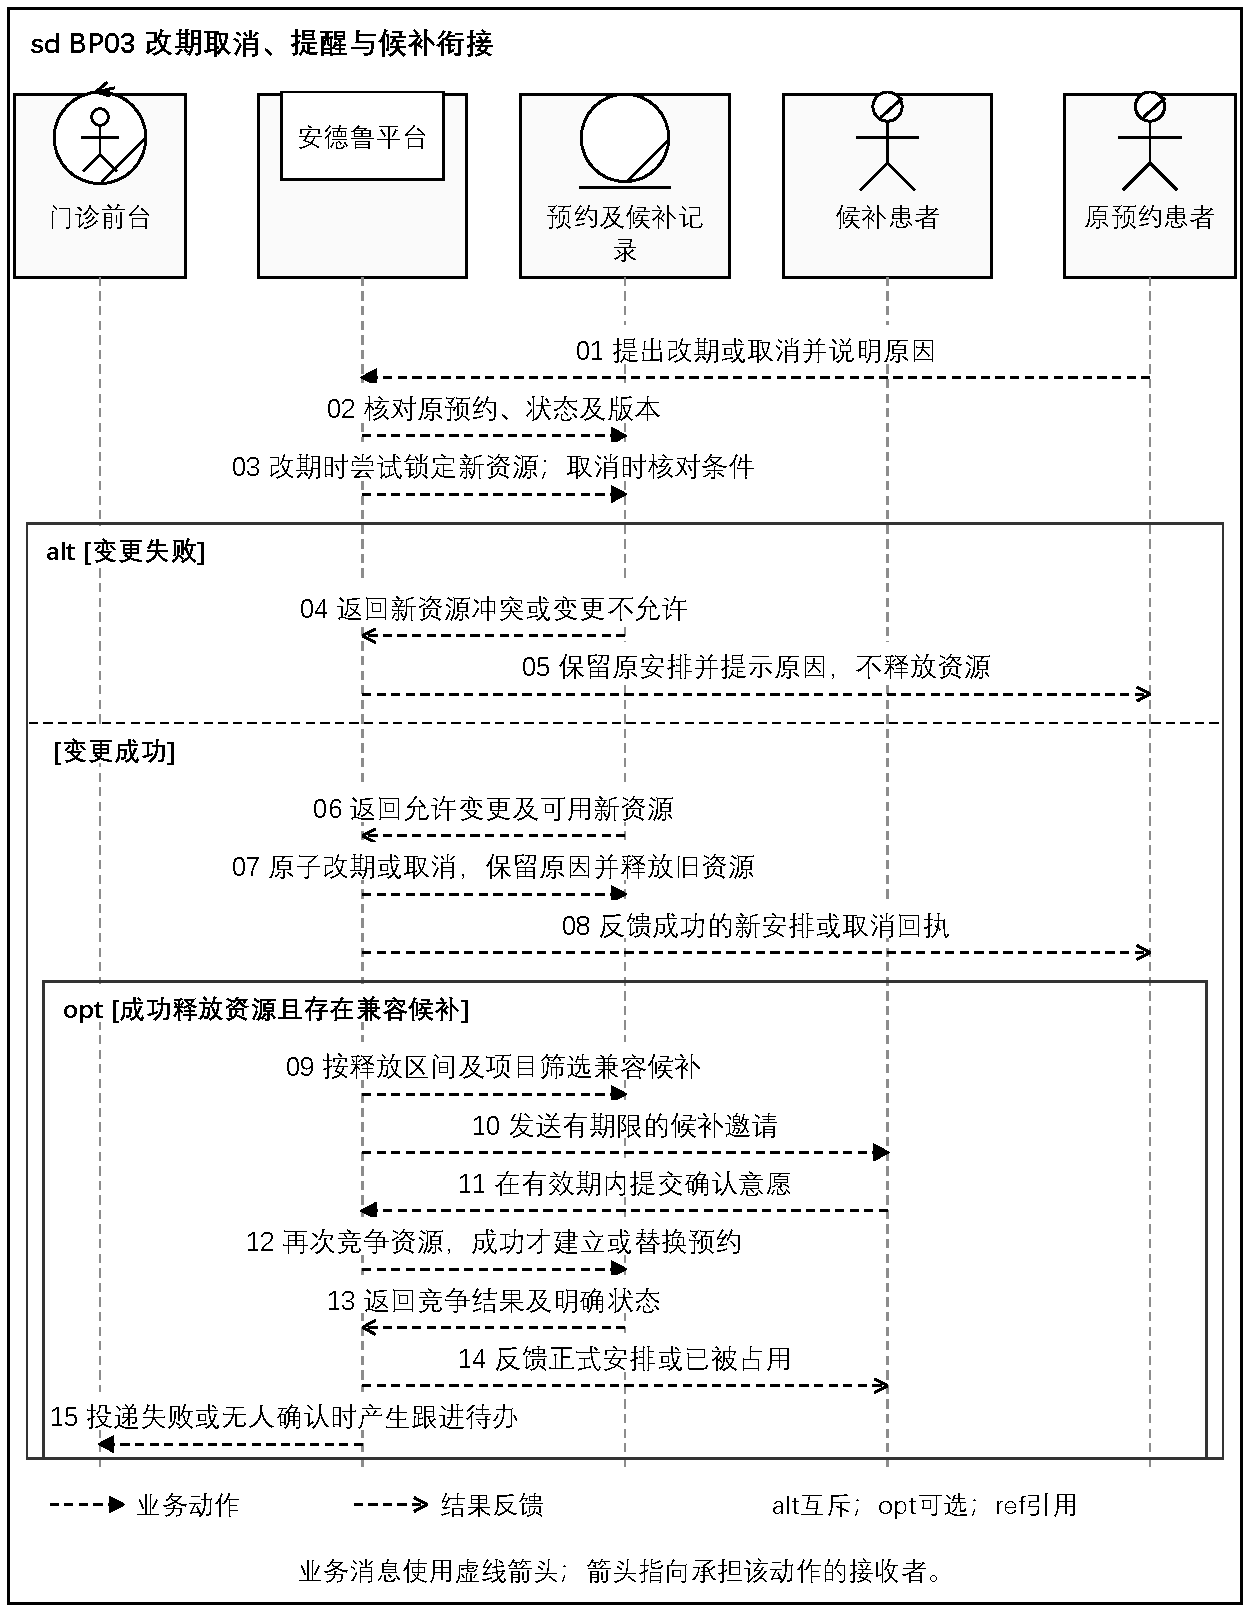
\includegraphics[width=\textwidth]{figures/BP03.pdf}
\caption{BP03 改期取消、提醒与候补衔接}\label{BP03}\end{figure}
\begin{figure}[H]\centering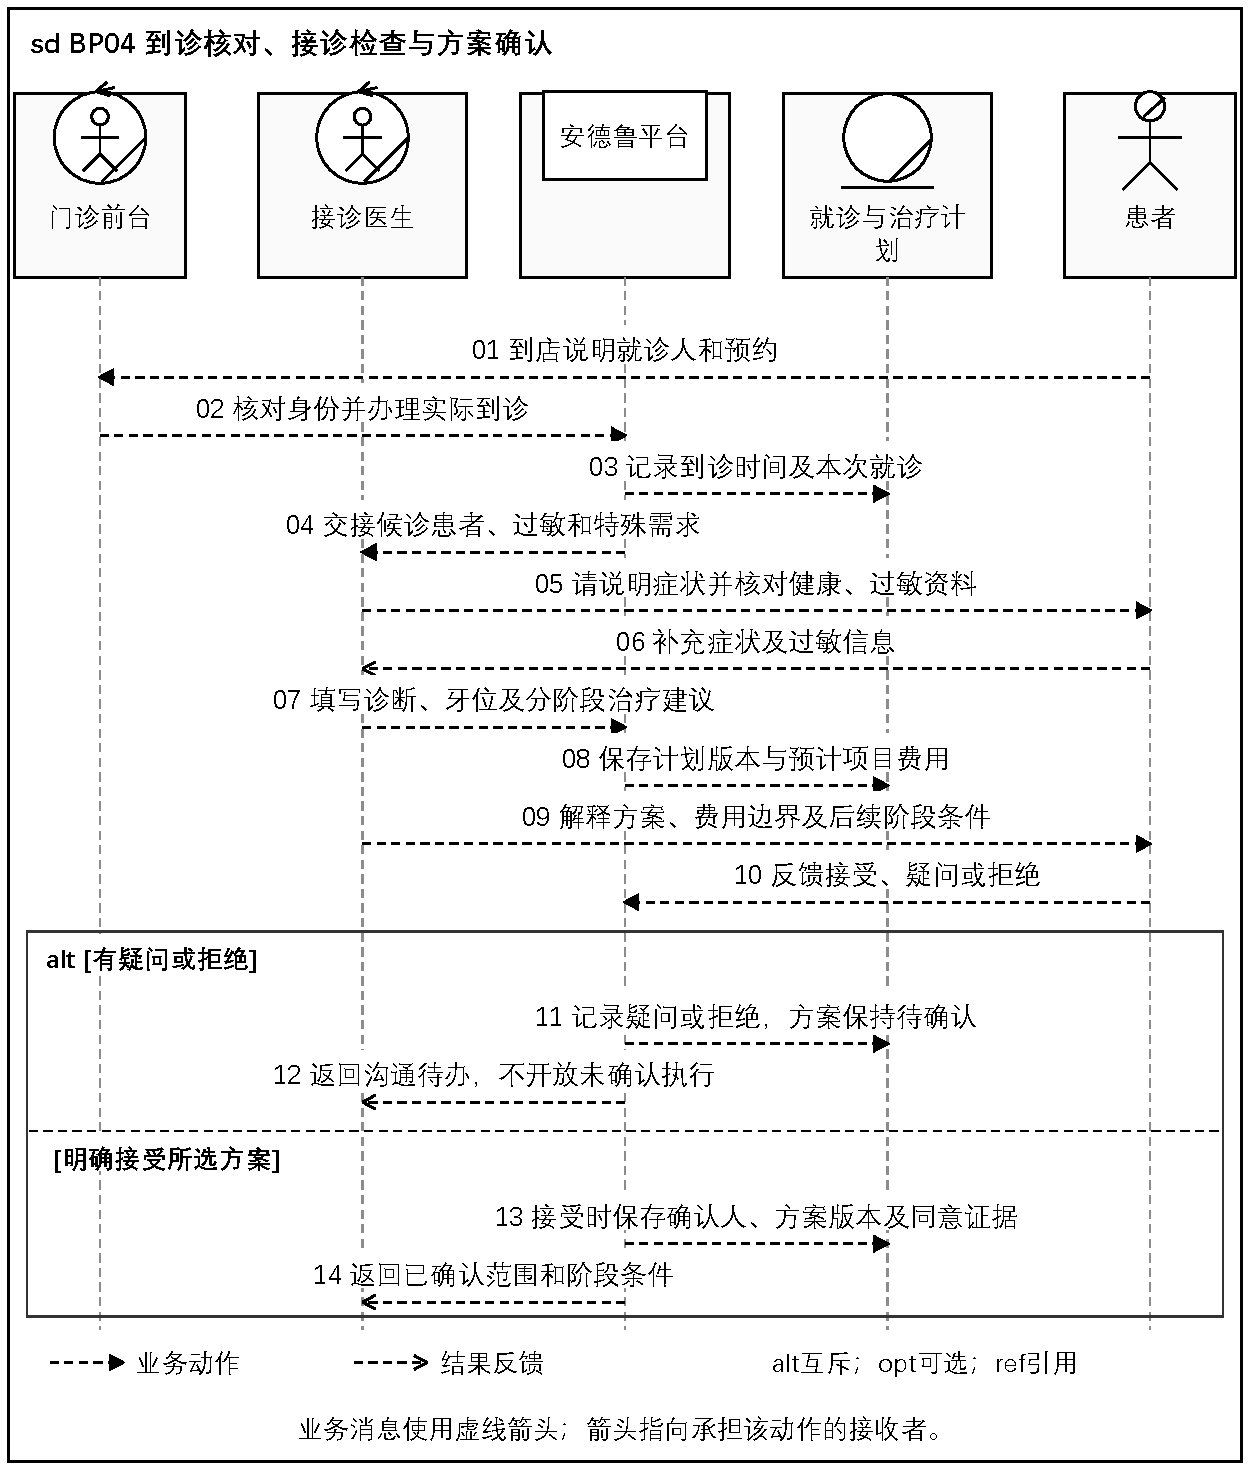
\includegraphics[width=\textwidth]{figures/BP04.pdf}
\caption{BP04 到诊核对、接诊检查与方案确认}\label{BP04}\end{figure}
\begin{figure}[H]\centering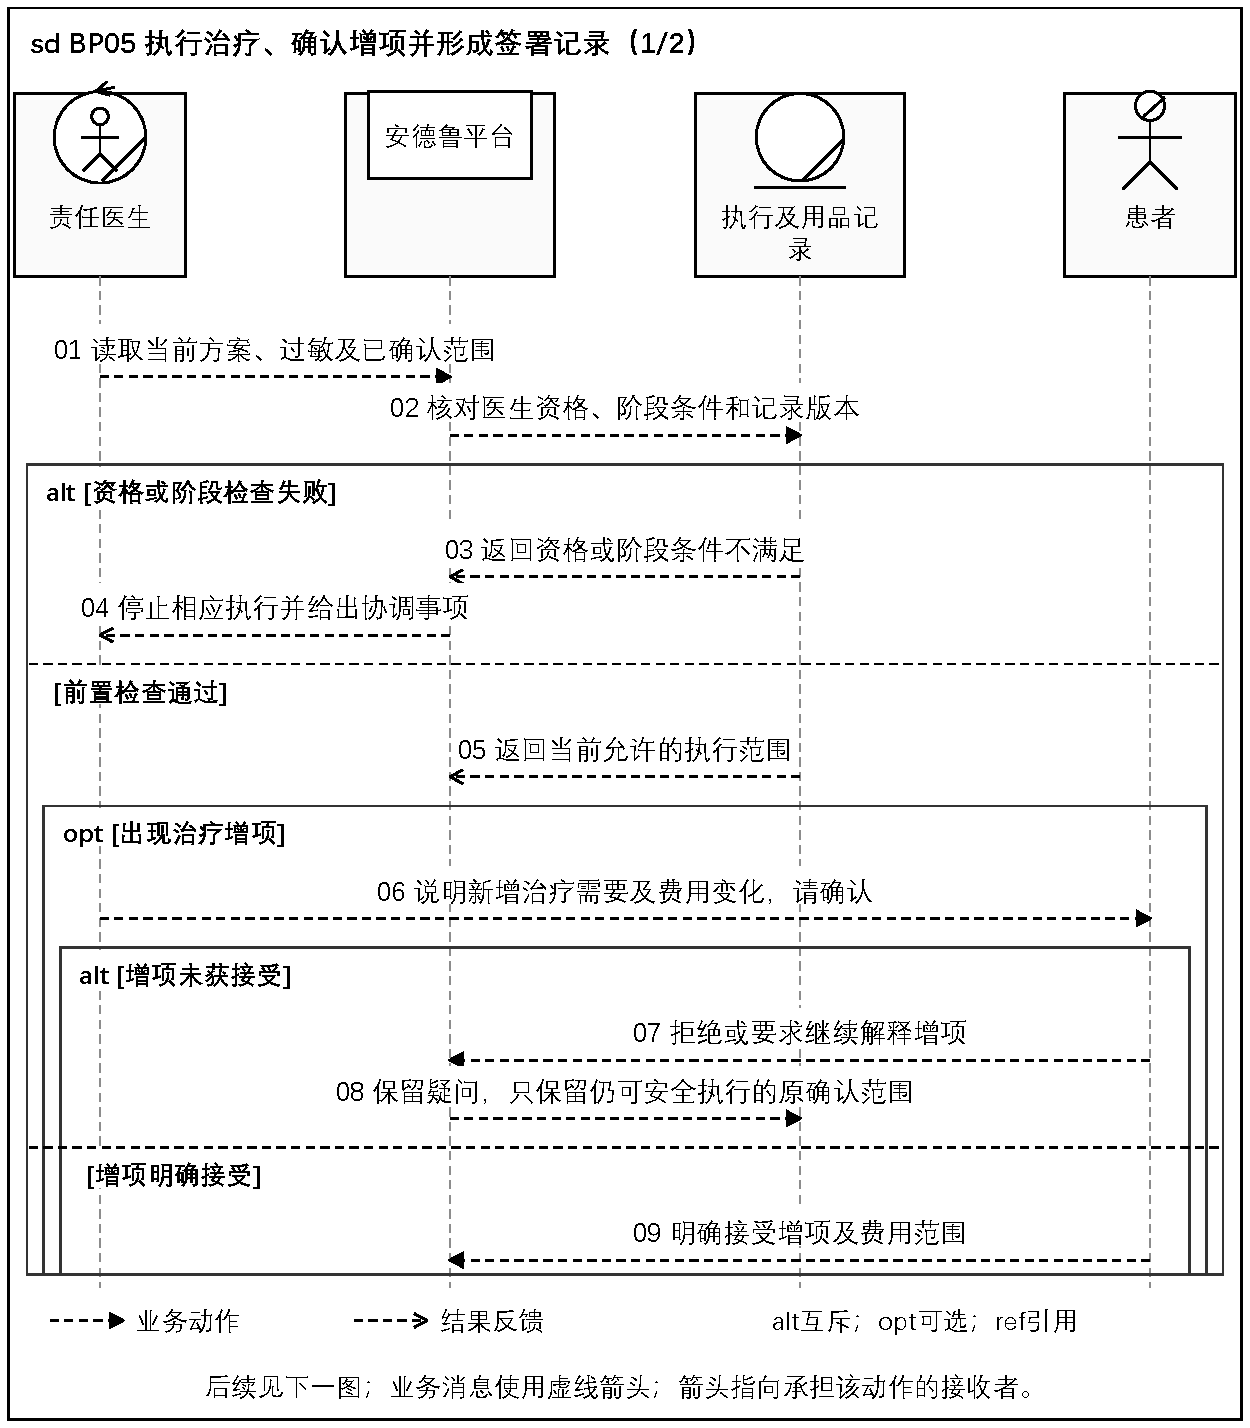
\includegraphics[width=\textwidth]{figures/BP05_1.pdf}
\caption{BP05 执行治疗、确认增项并形成签署记录（1/2）}\label{BP05_1}\end{figure}
\begin{figure}[H]\centering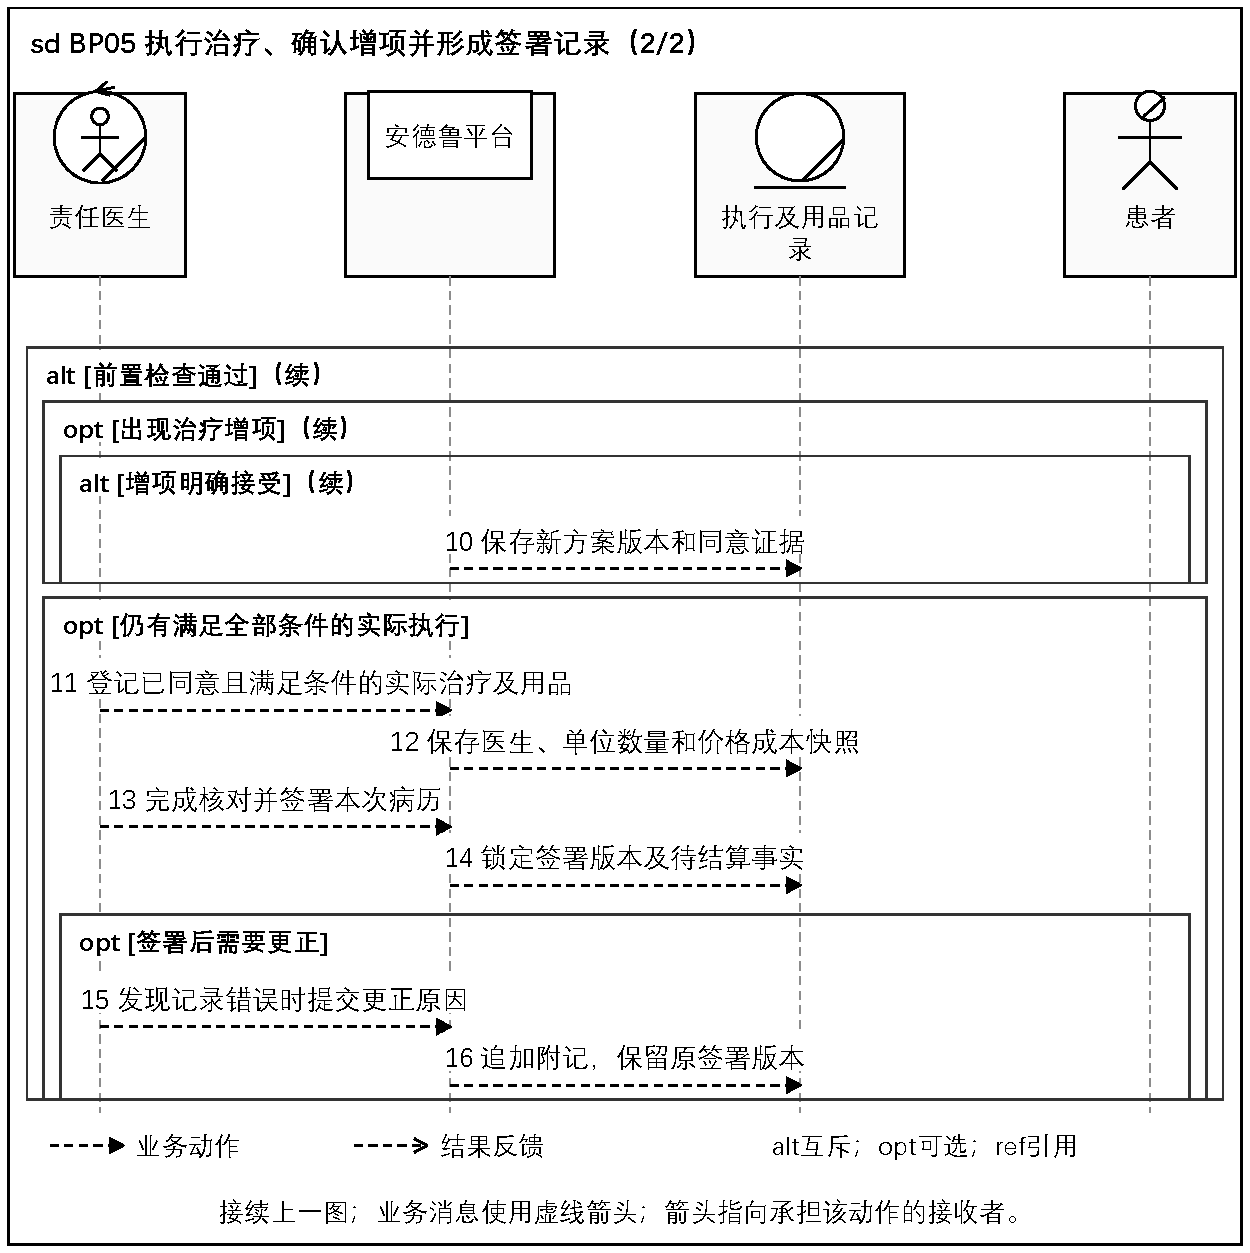
\includegraphics[width=\textwidth]{figures/BP05_2.pdf}
\caption{BP05 执行治疗、确认增项并形成签署记录（2/2）}\label{BP05_2}\end{figure}
\begin{figure}[H]\centering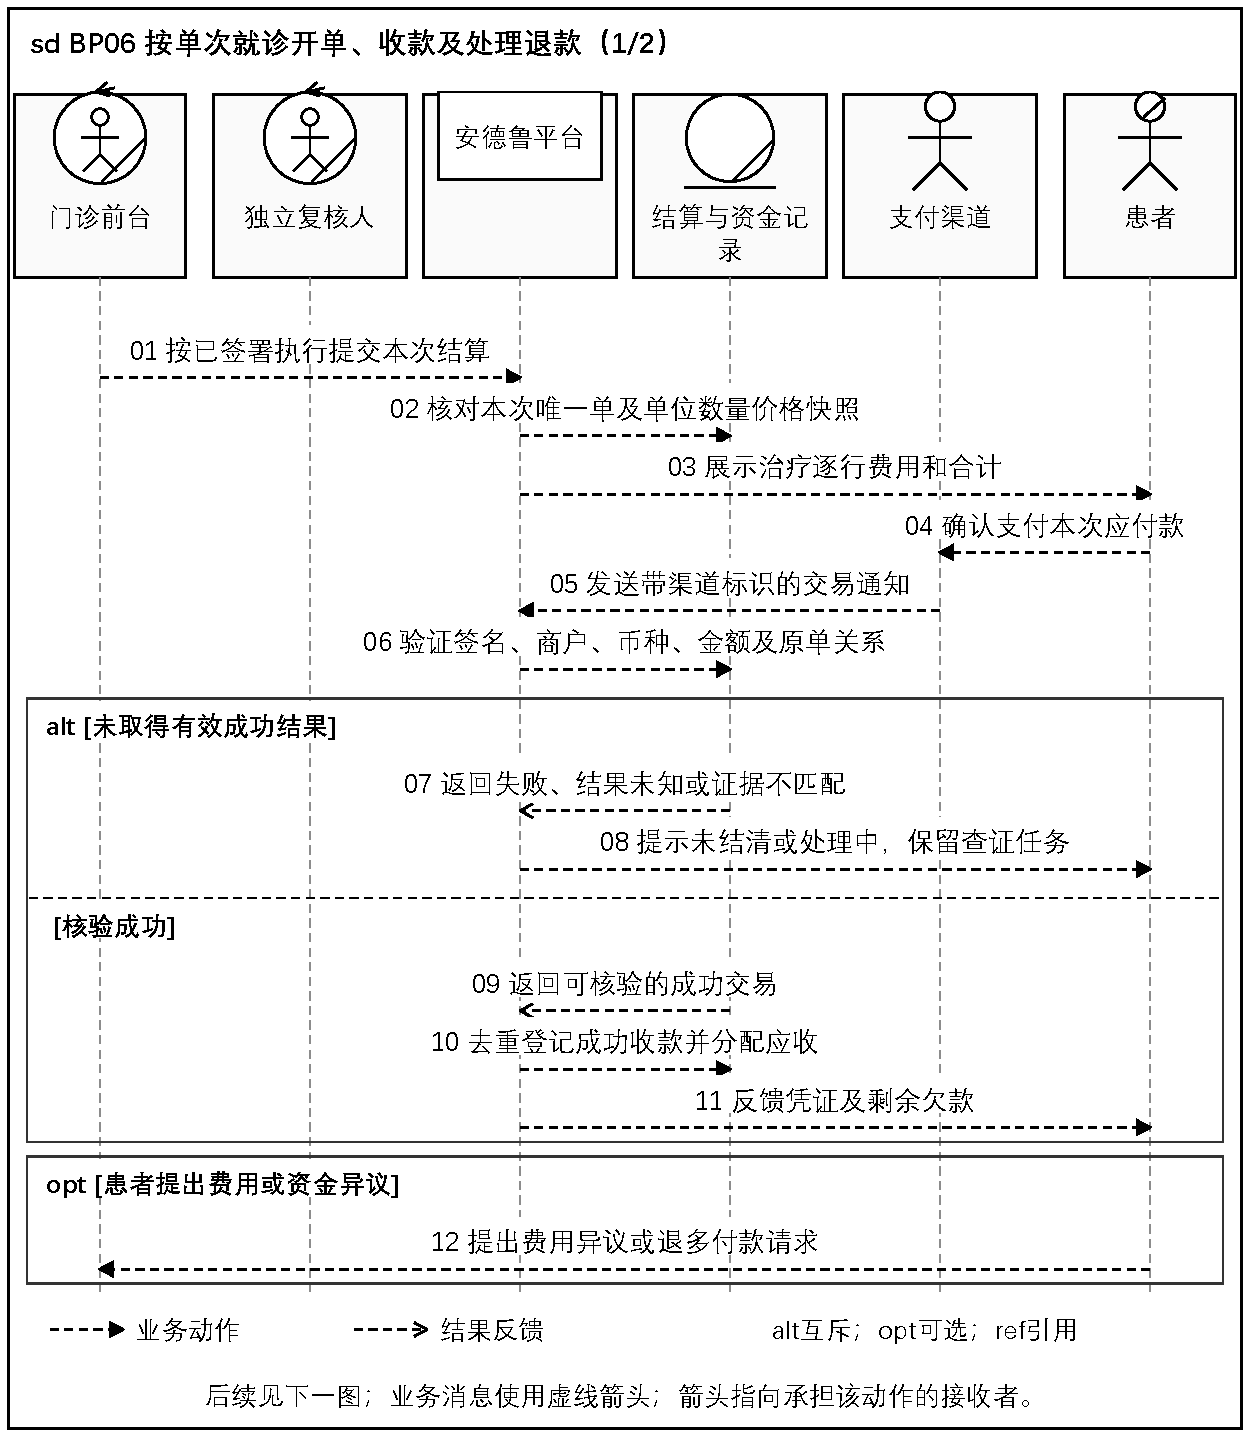
\includegraphics[width=\textwidth]{figures/BP06_1.pdf}
\caption{BP06 按单次就诊开单、收款及处理退款（1/2）}\label{BP06_1}\end{figure}
\begin{figure}[H]\centering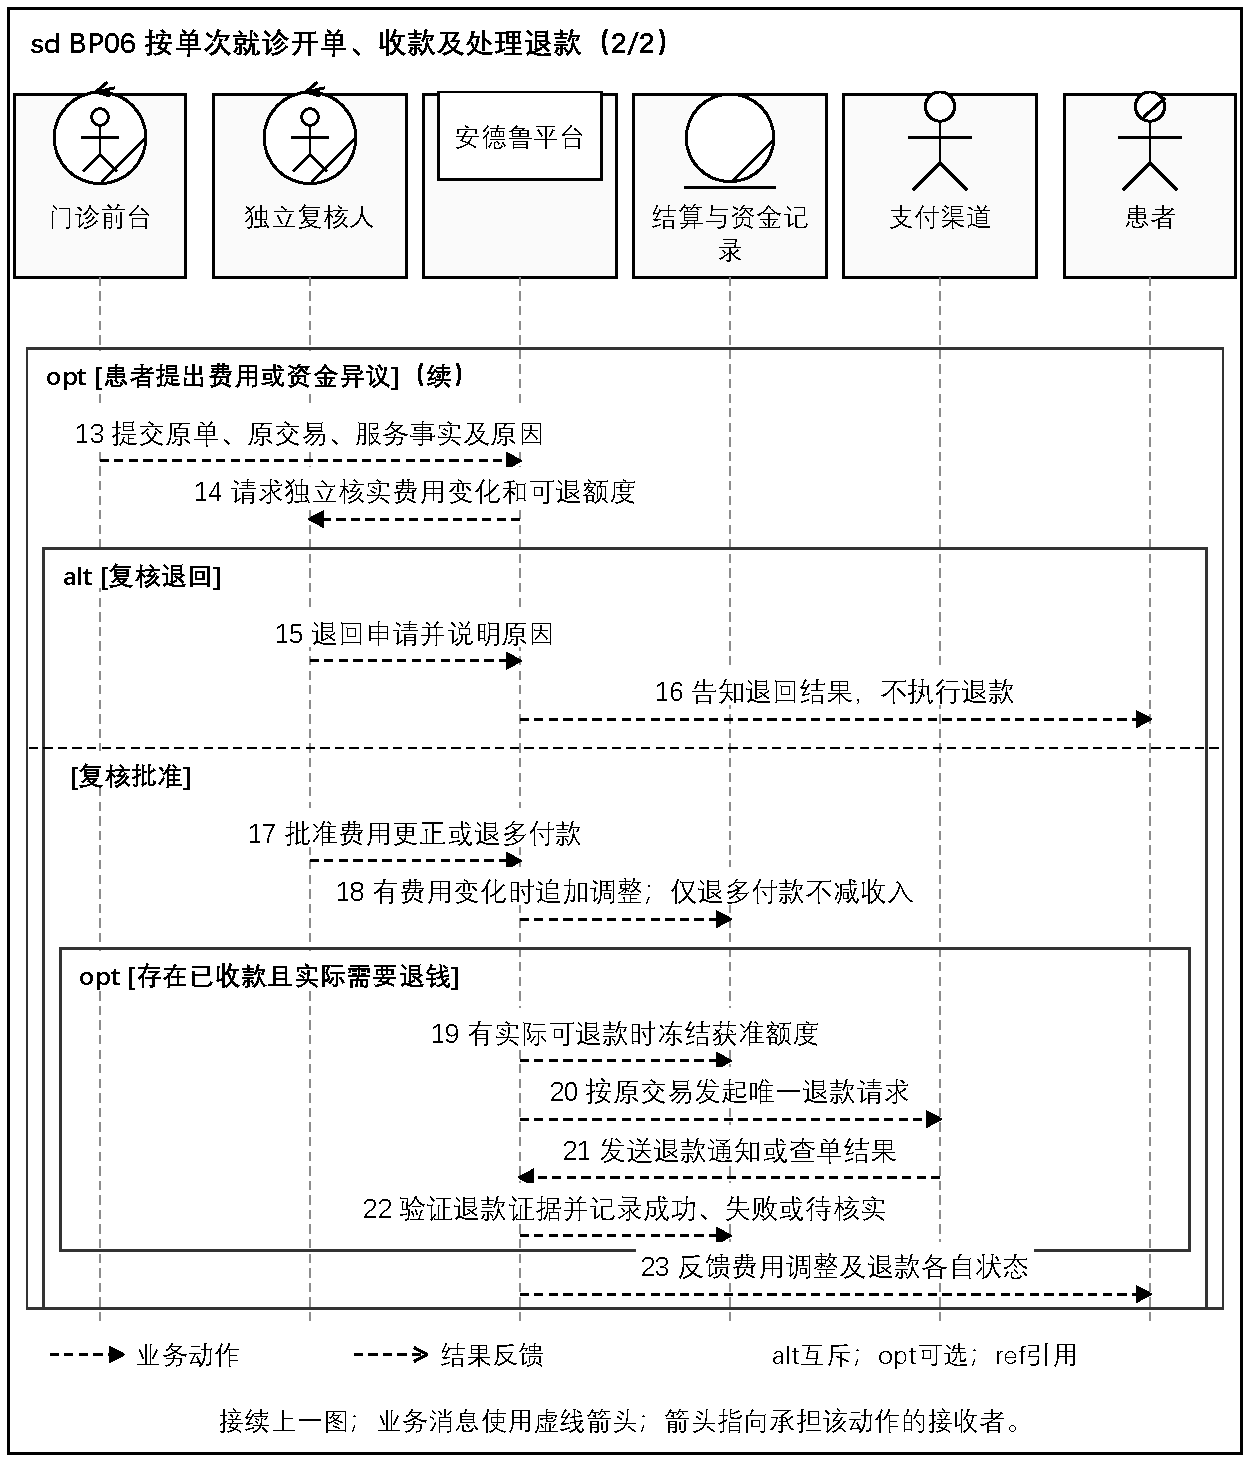
\includegraphics[width=\textwidth]{figures/BP06_2.pdf}
\caption{BP06 按单次就诊开单、收款及处理退款（2/2）}\label{BP06_2}\end{figure}
\begin{figure}[H]\centering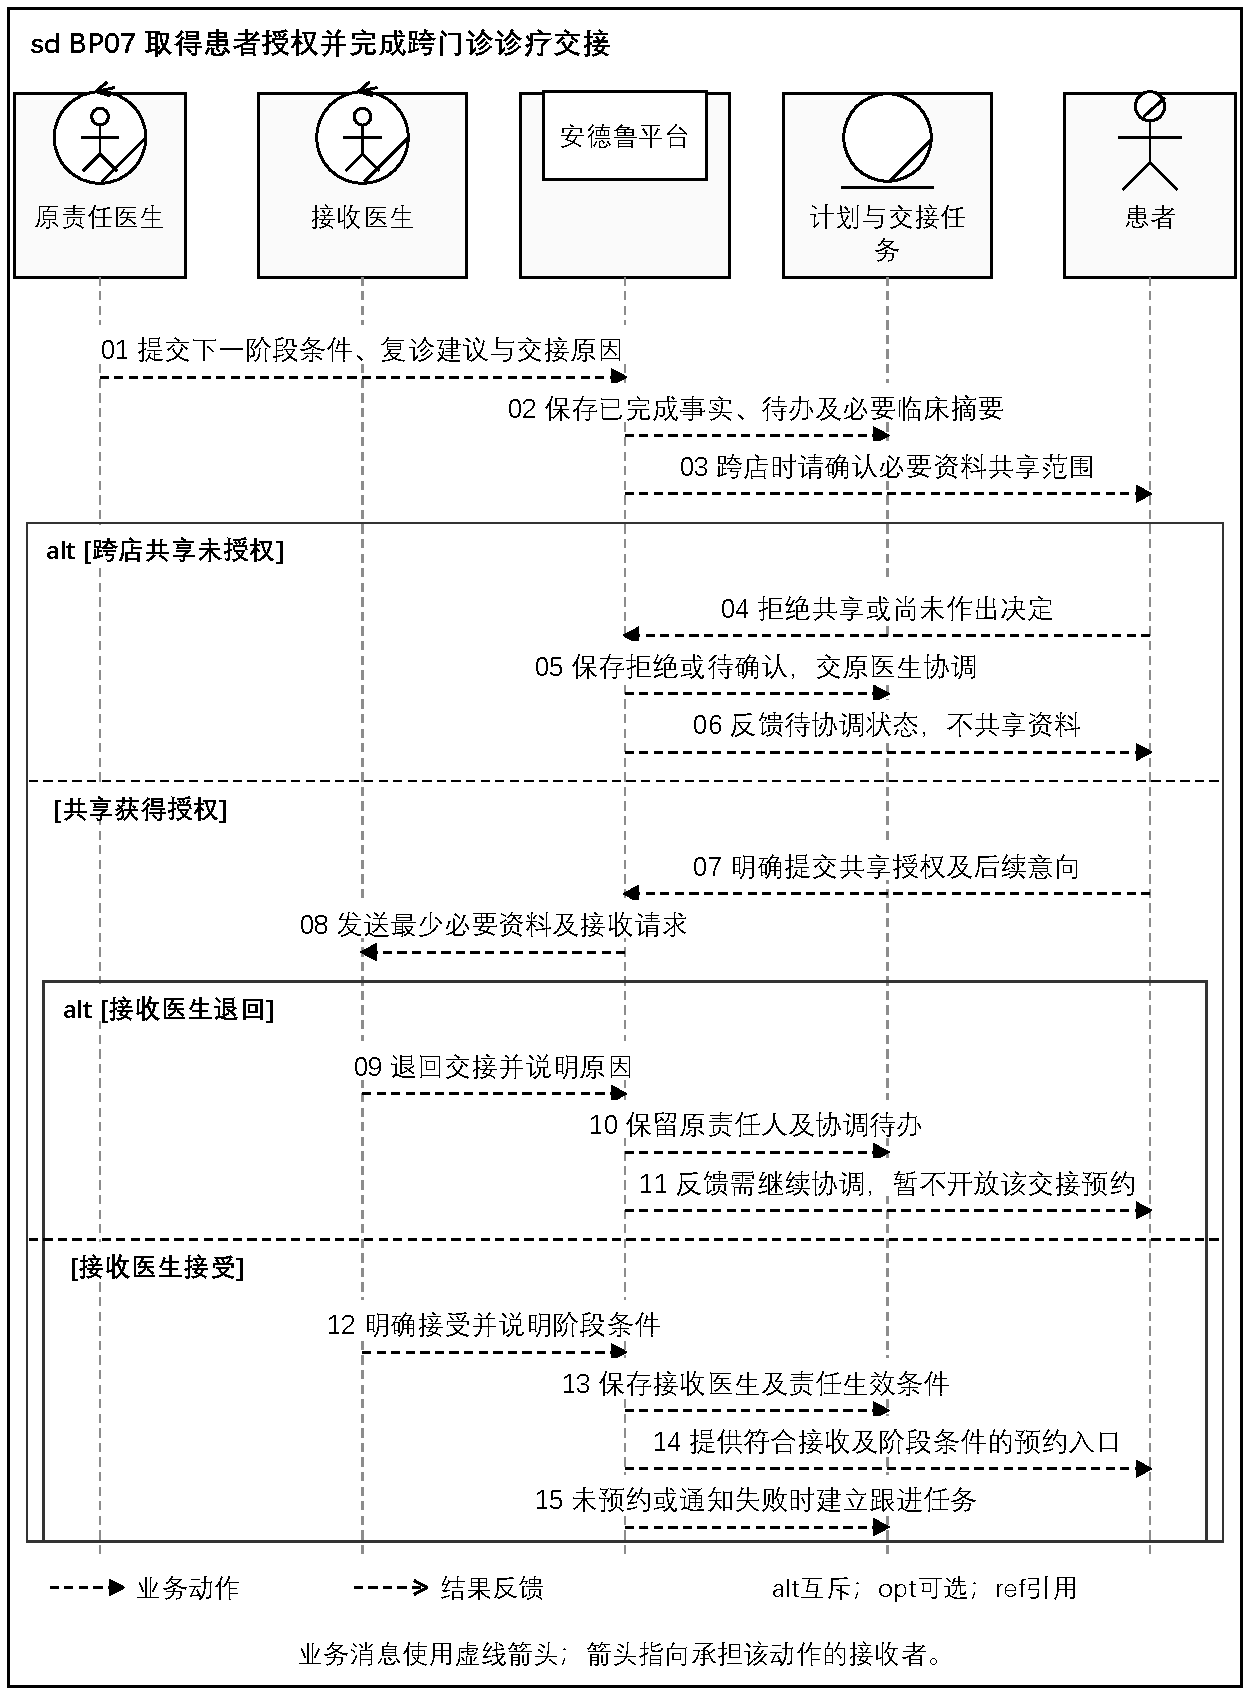
\includegraphics[width=\textwidth]{figures/BP07.pdf}
\caption{BP07 取得患者授权并完成跨门诊诊疗交接}\label{BP07}\end{figure}
\Needspace{562pt}
\subsection{门诊与总部经营支撑}
\begin{figure}[H]\centering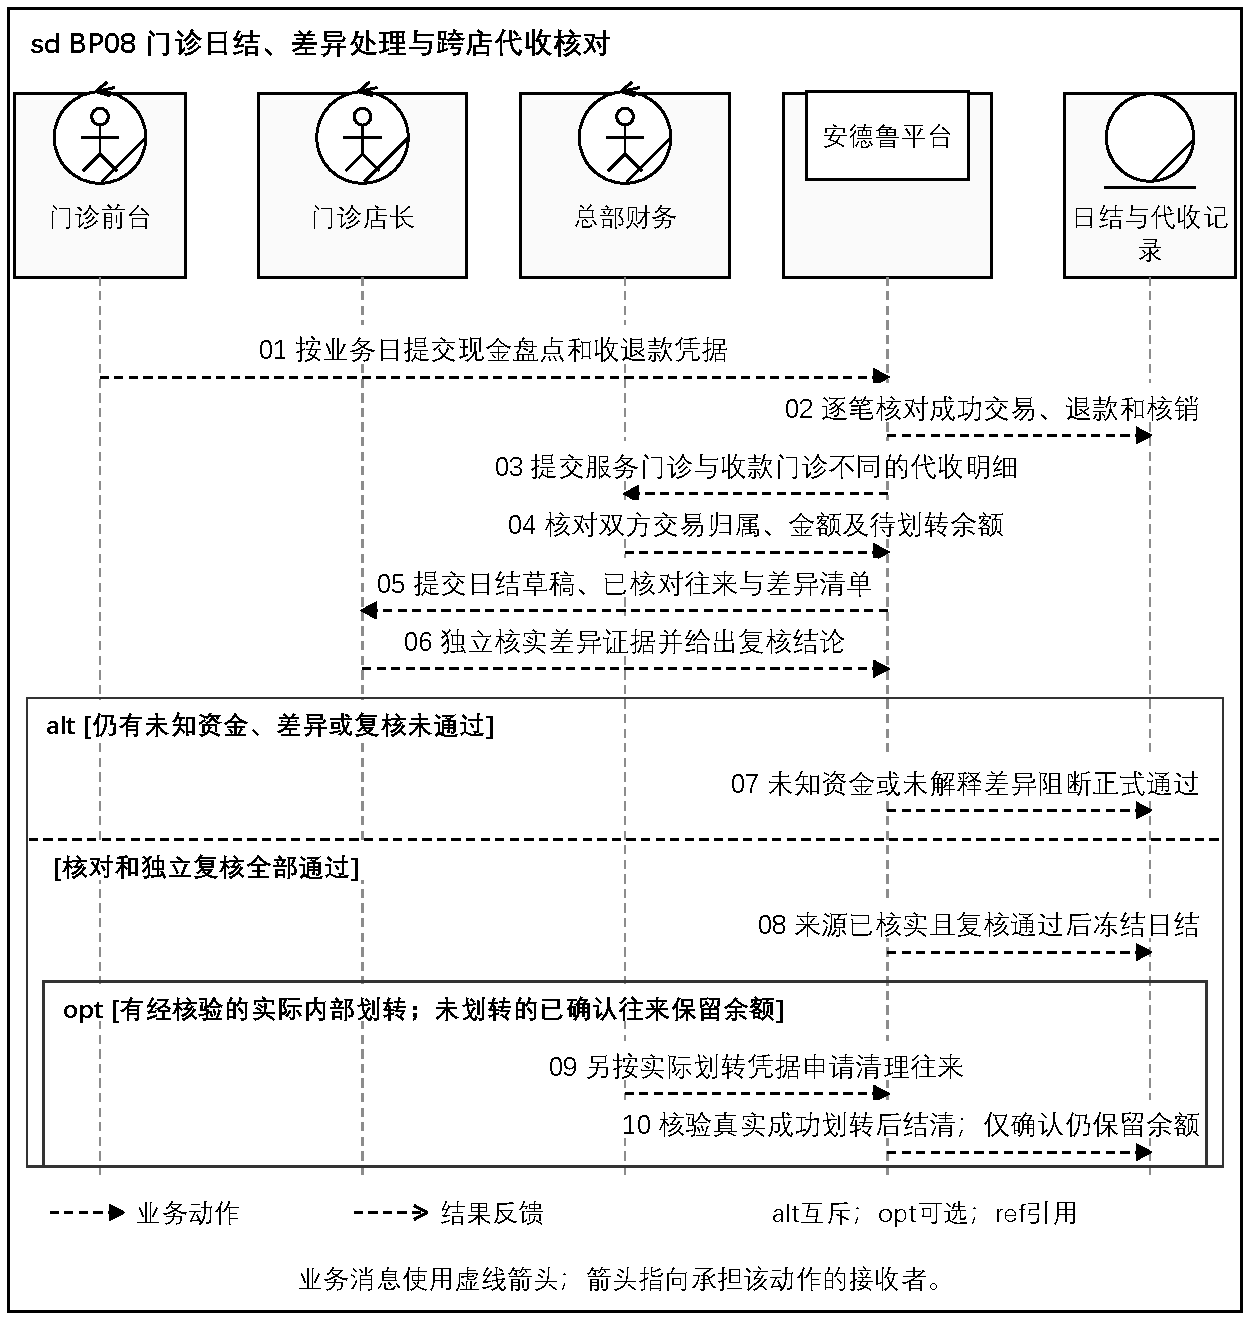
\includegraphics[width=\textwidth]{figures/BP08.pdf}
\caption{BP08 门诊日结、差异处理与跨店代收核对}\label{BP08}\end{figure}
\begin{figure}[H]\centering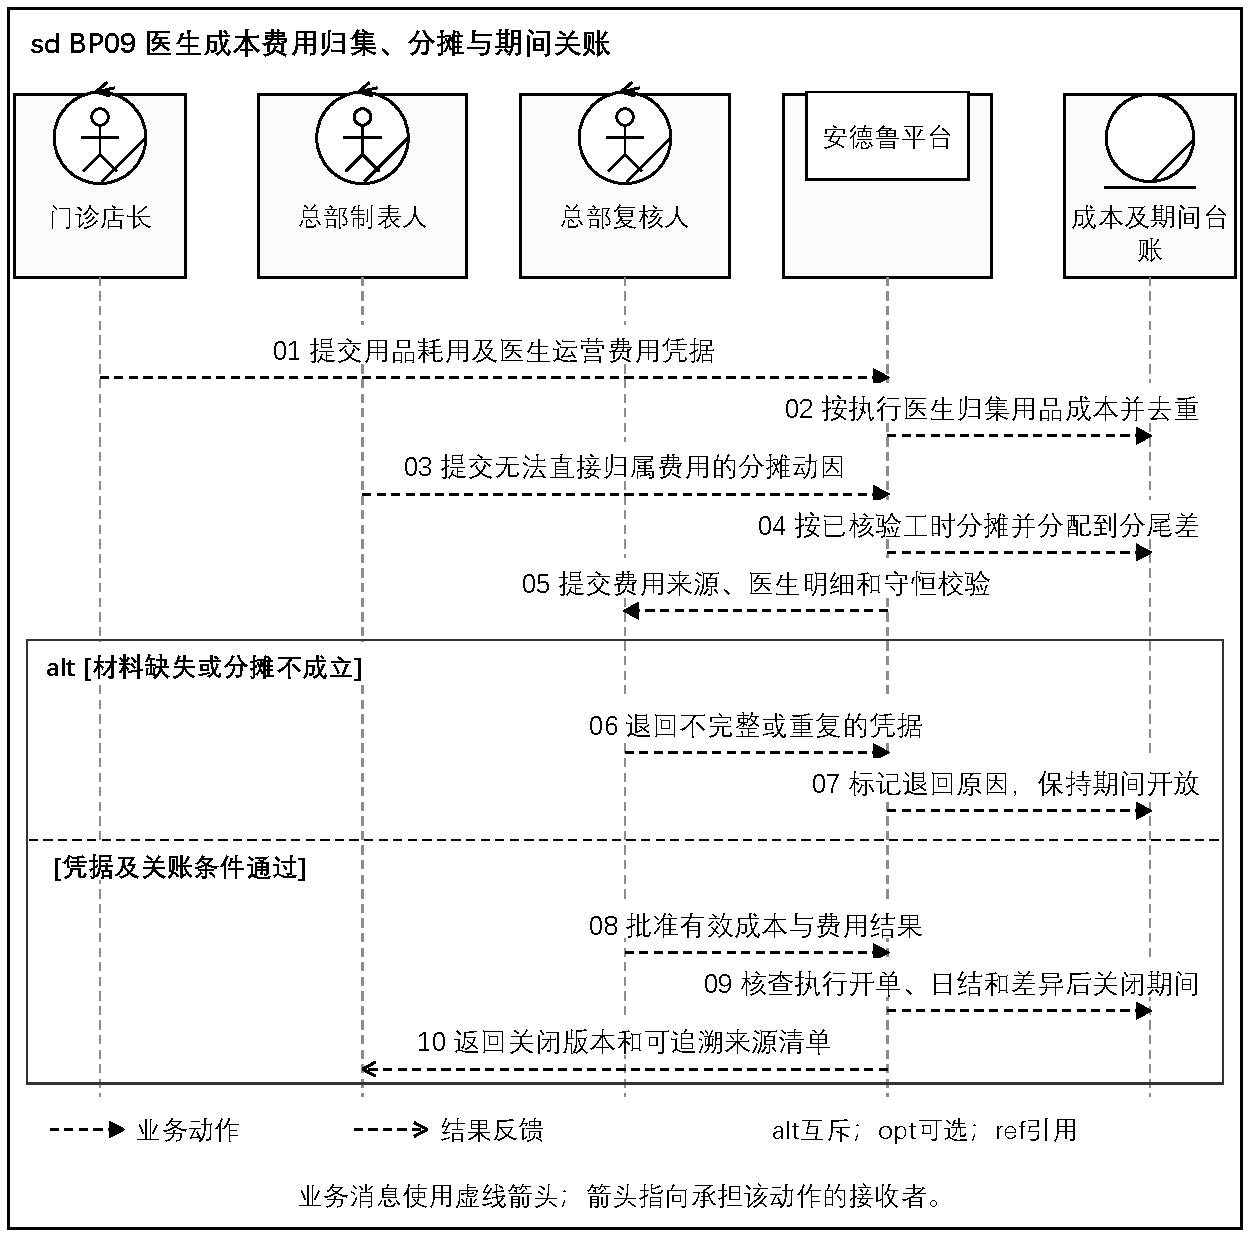
\includegraphics[width=\textwidth]{figures/BP09.pdf}
\caption{BP09 医生成本费用归集、分摊与期间关账}\label{BP09}\end{figure}
\begin{figure}[H]\centering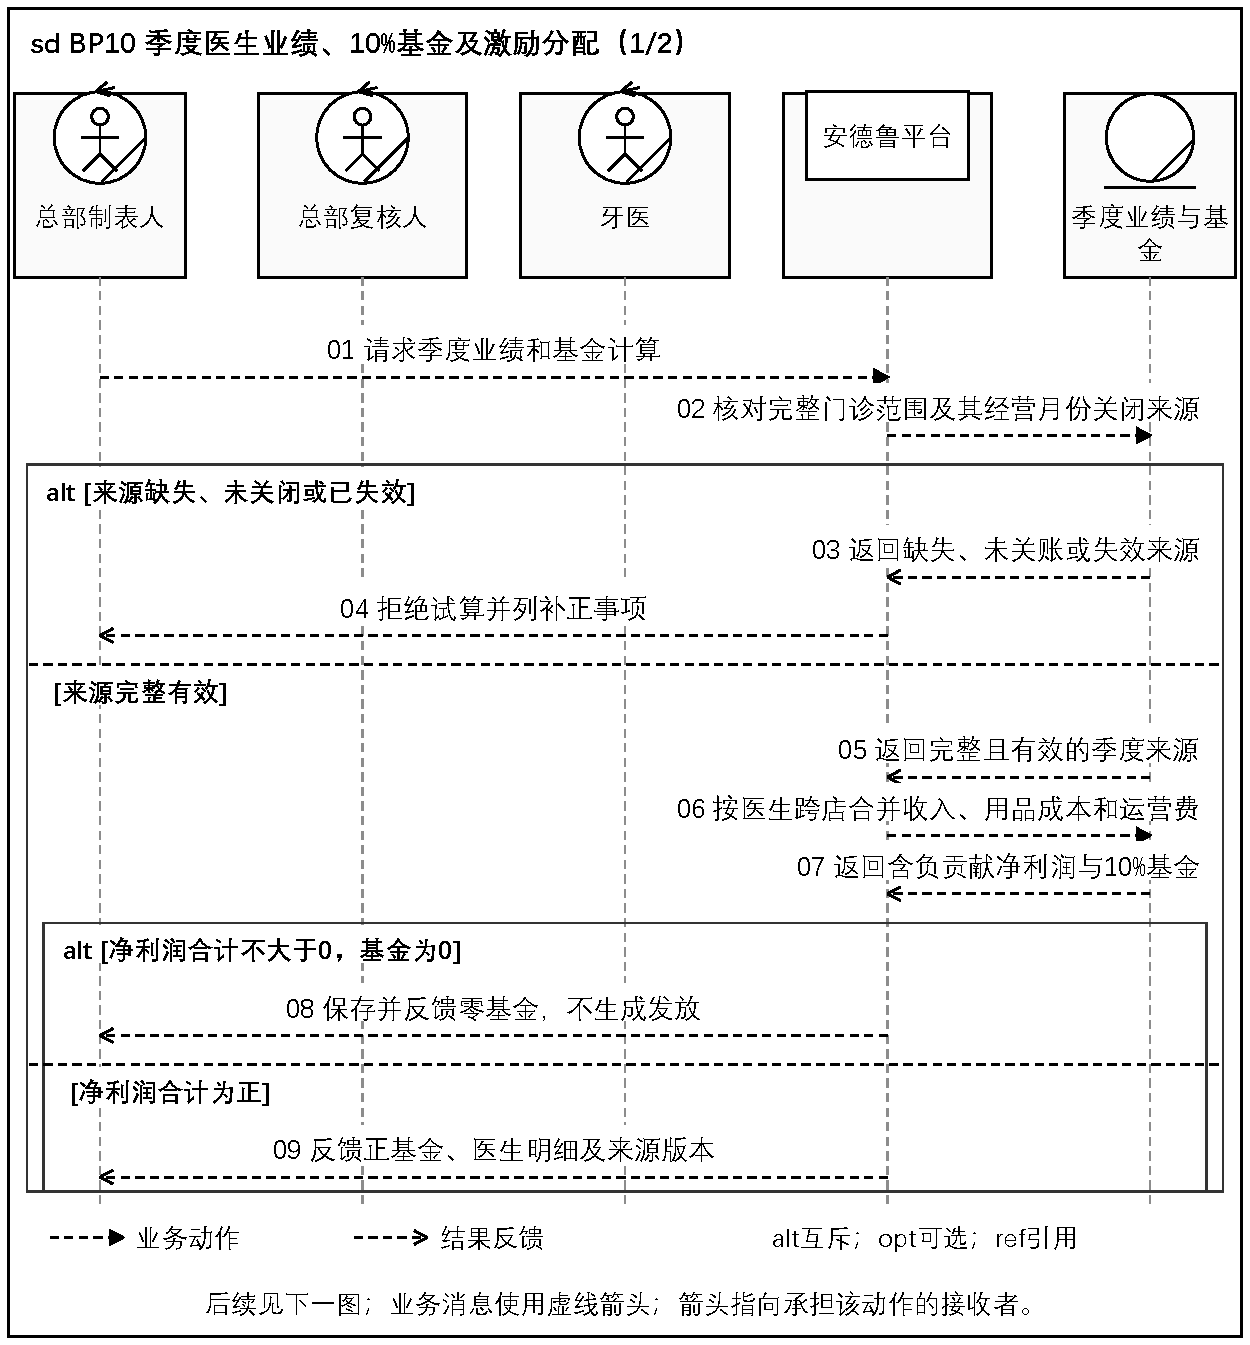
\includegraphics[width=\textwidth]{figures/BP10_1.pdf}
\caption{BP10 季度医生业绩、10\%基金及激励分配（1/2）}\label{BP10_1}\end{figure}
\begin{figure}[H]\centering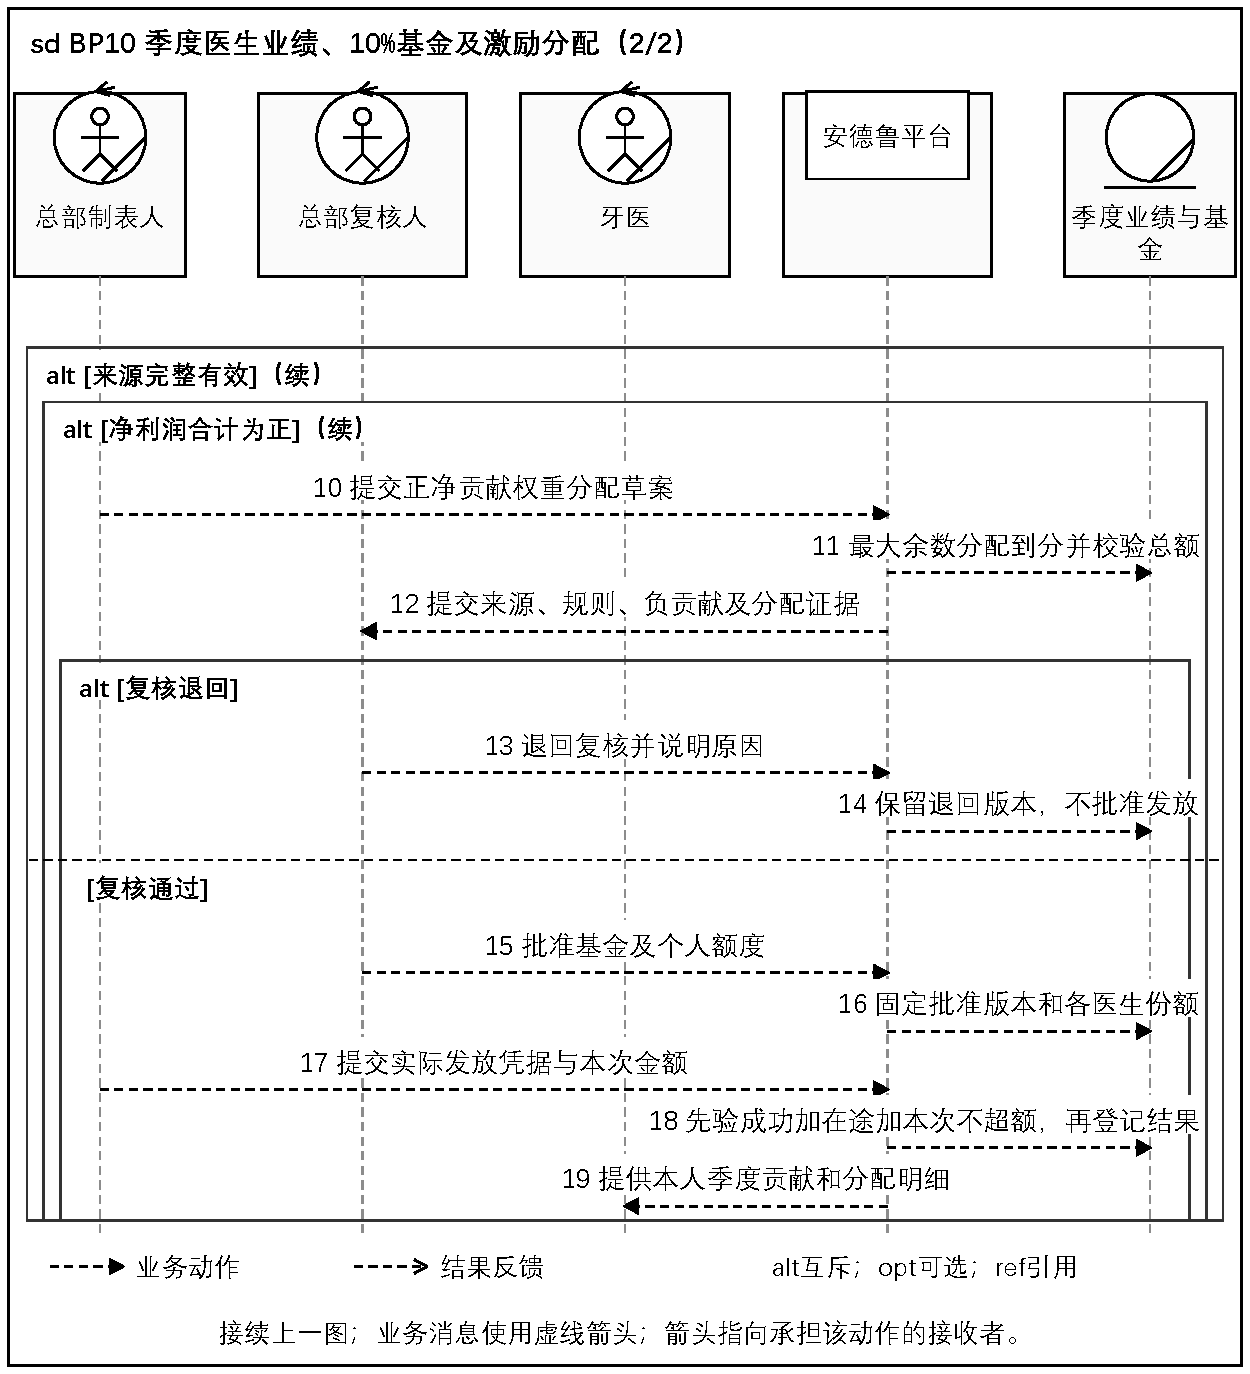
\includegraphics[width=\textwidth]{figures/BP10_2.pdf}
\caption{BP10 季度医生业绩、10\%基金及激励分配（2/2）}\label{BP10_2}\end{figure}
\par\noindent\begin{minipage}{\textwidth}
{\fontsize{10.5pt}{13.2pt}\selectfont\setlength{\tabcolsep}{0pt}\renewcommand{\arraystretch}{1.08}
\captionof{table}{跨环节交接条件}\label{tab70}
\begin{tabular}{@{}p{3.040cm}@{\hspace{0.16cm}}p{6.640cm}@{\hspace{0.16cm}}p{5.440cm}@{}}
\toprule
\bfseries \Cell{交接} & \bfseries \Cell{必须提供} & \bfseries \Cell{接收者的确认}\\\midrule
\Cell{预约→到诊} & \Cell{患者身份、实际门诊、接诊医生、时段与特殊需求} & \Cell{前台核对实际到诊，医生确认接诊。}\\[1pt]
\Cell{方案→执行} & \Cell{有效方案版本、过敏核对及同意范围} & \Cell{医生核对阶段条件；增项重新确认。}\\[1pt]
\Cell{执行→结算} & \Cell{签署执行行、标准单位、数量、单价和医生} & \Cell{前台核对本次就诊唯一单据及费用。}\\[1pt]
\Cell{收款→日结} & \Cell{成功交易、分配、退款状态与收款地点} & \Cell{店长独立复核差异，未知交易不能当成功。}\\[1pt]
\Cell{门诊→总部} & \Cell{已复核资金、成本来源与医生归属} & \Cell{总部确认期间完整性及分摊守恒。}\\[1pt]
\Cell{季度结果→基金→发放} & \Cell{来源关闭版本、医生净利润、基金及个人分配} & \Cell{独立复核人批准，发放登记引用真实凭据。}\\[1pt]
\bottomrule\end{tabular}
}\end{minipage}\par\vspace{6pt}
\Needspace{678pt}
\section{系统用例与需求规约}
系统执行者包括患者及合法代办人、前台、医生、店长和总部授权人员。业务用例关心患者获得的服务，系统用例进一步说明这些人员怎样使用平台完成工作。支付和通知属于辅助系统，不获得内部岗位权限。系统用例图中的实线只表示参与，业务先后以规约和业务序列为准。\par
\begin{figure}[H]\centering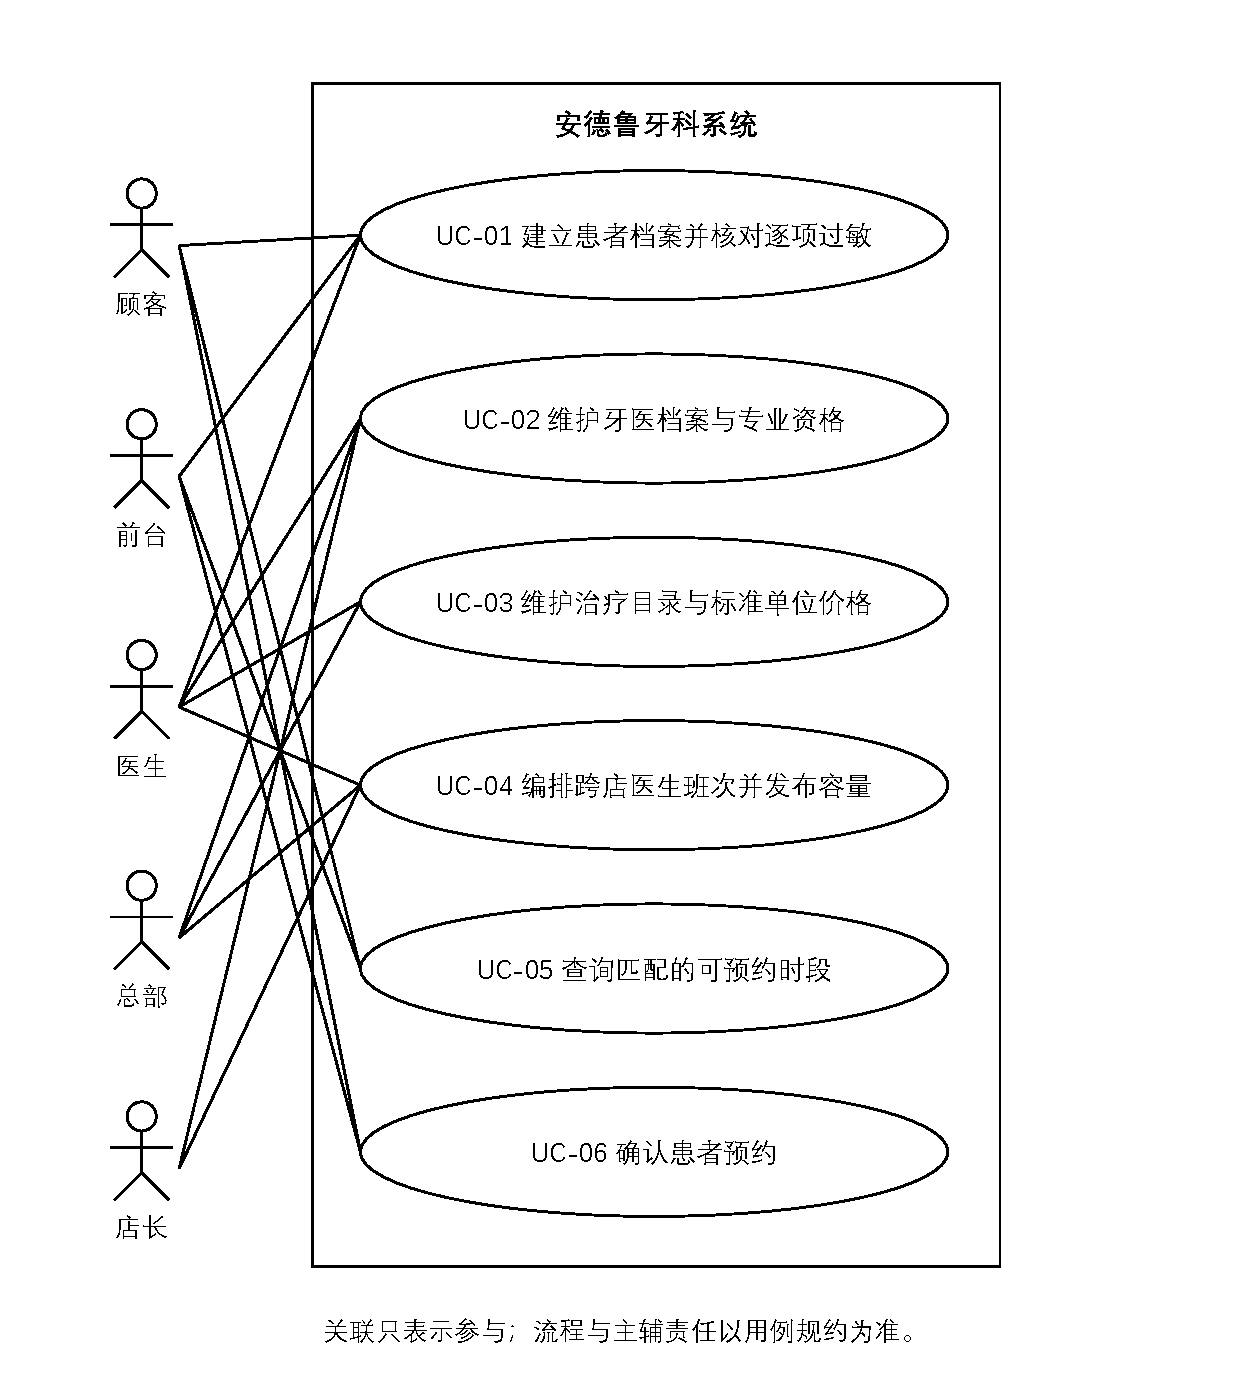
\includegraphics[width=\textwidth]{figures/uc_overview_1.pdf}
\caption{系统用例总览 1}\label{uc_overview_1}\end{figure}
\begin{figure}[H]\centering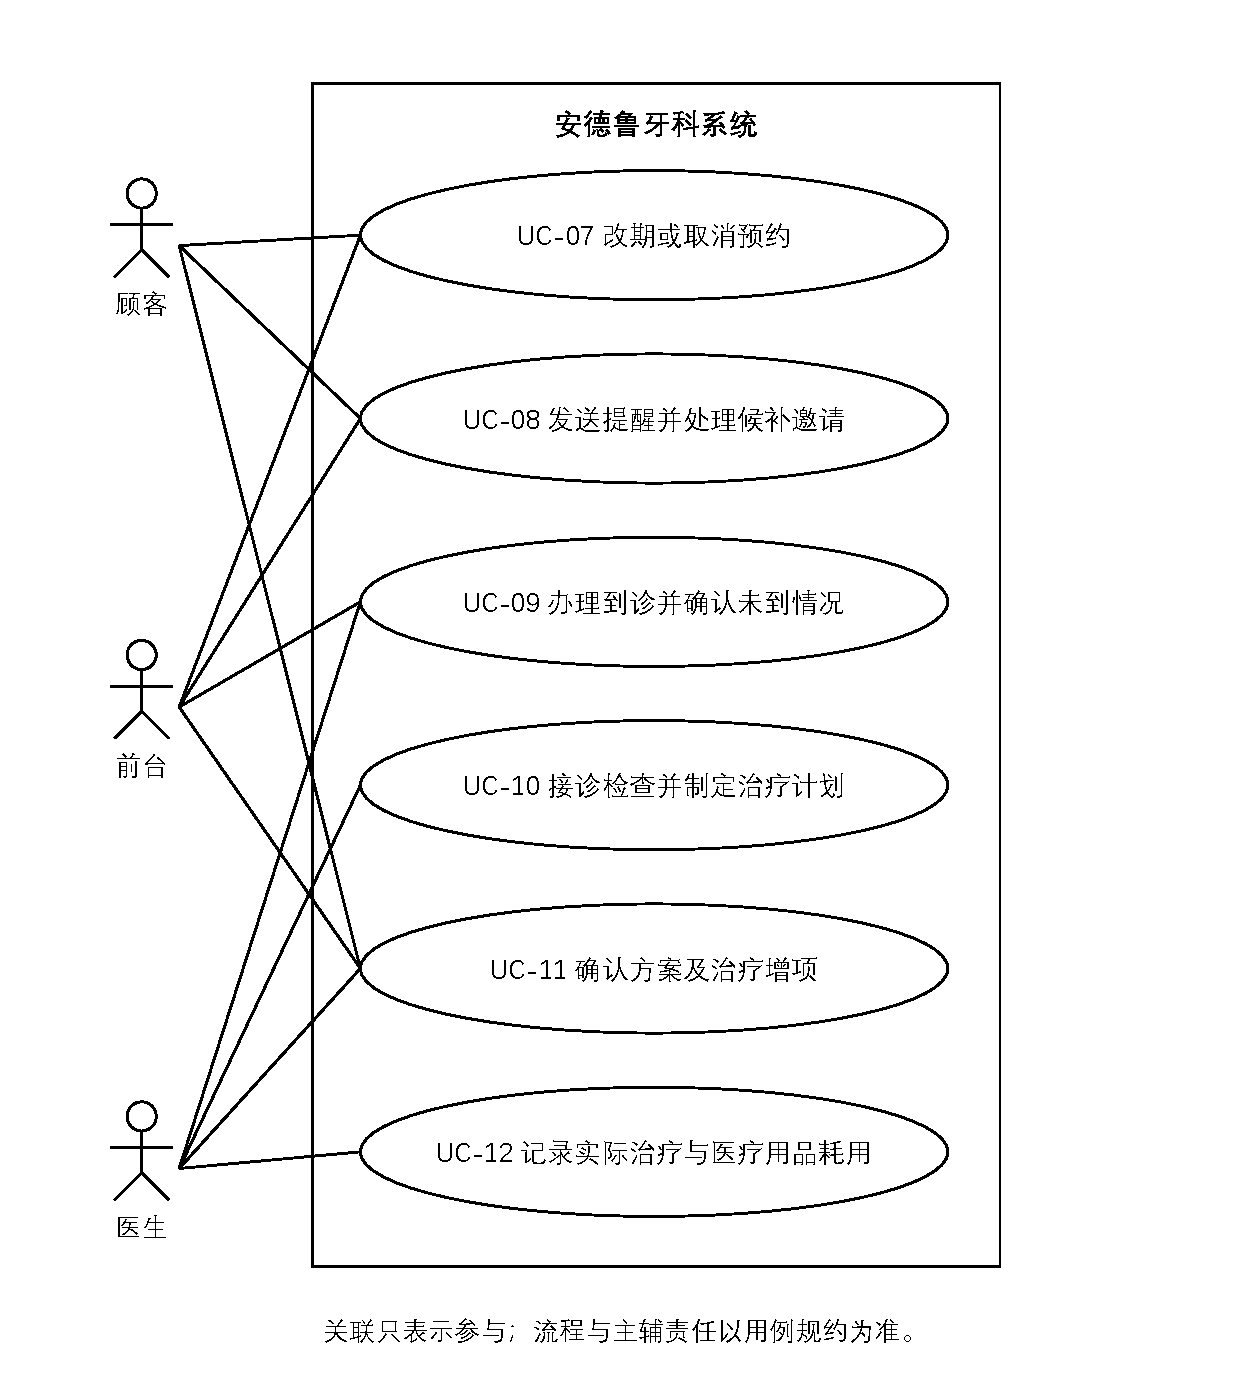
\includegraphics[width=\textwidth]{figures/uc_overview_2.pdf}
\caption{系统用例总览 2}\label{uc_overview_2}\end{figure}
\begin{figure}[H]\centering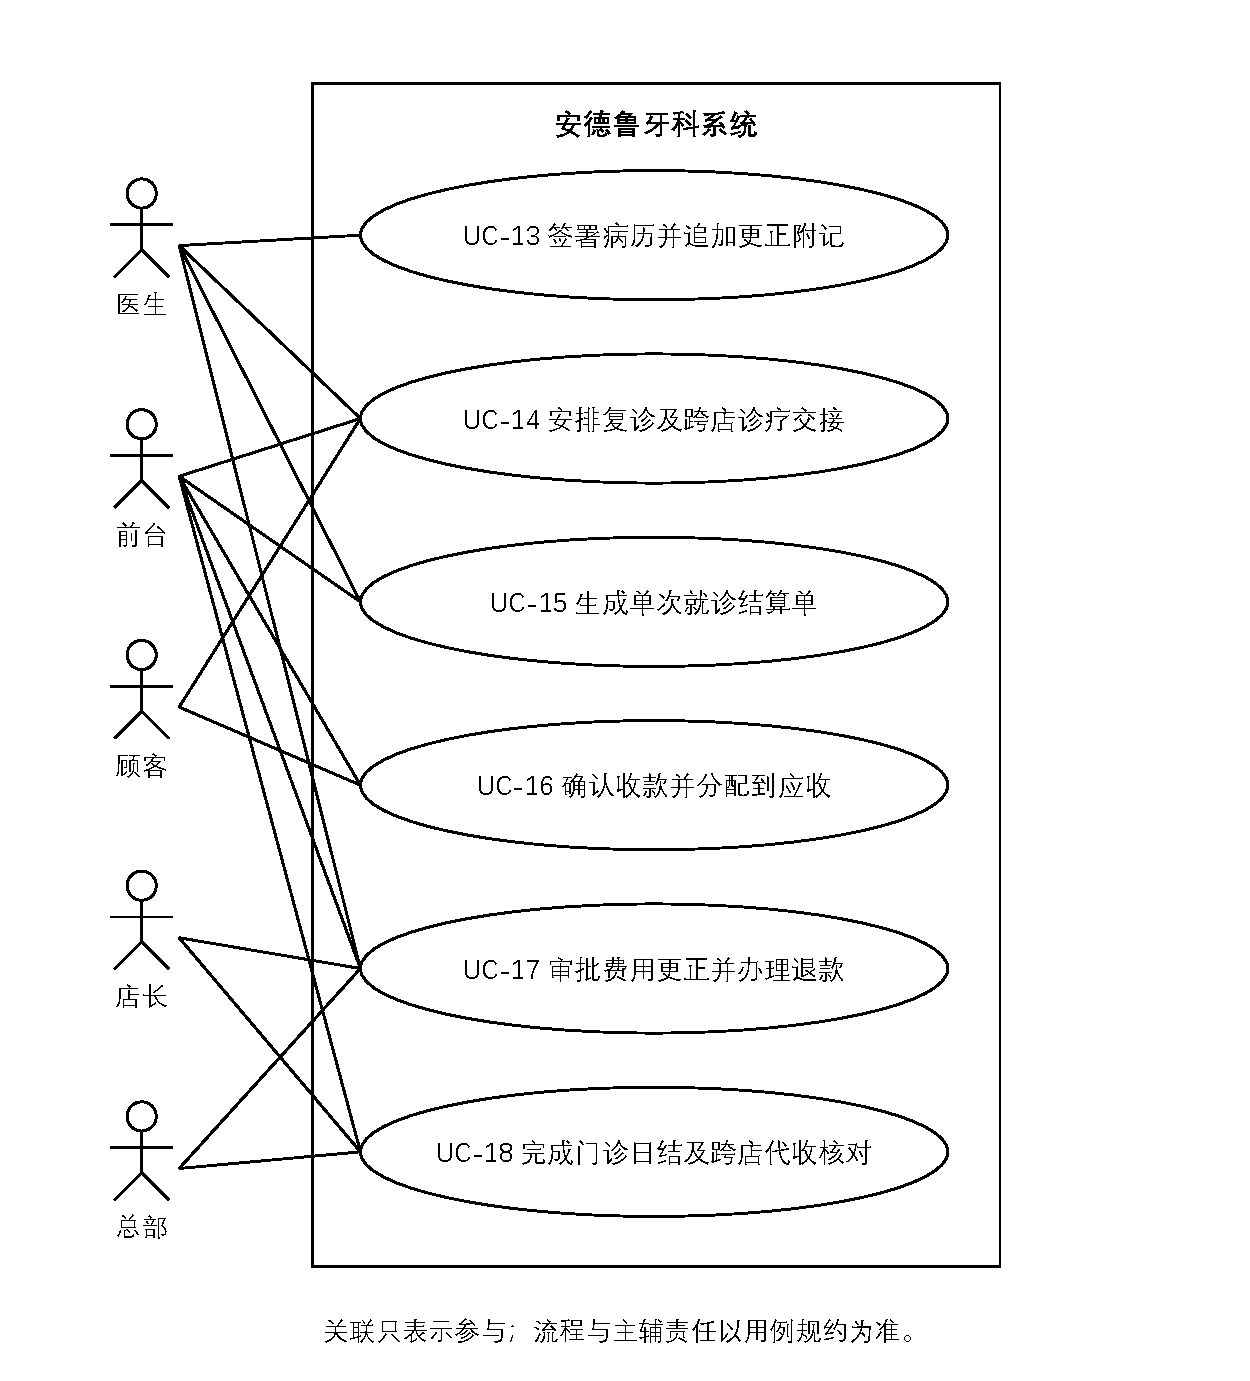
\includegraphics[width=\textwidth]{figures/uc_overview_3.pdf}
\caption{系统用例总览 3}\label{uc_overview_3}\end{figure}
\begin{figure}[H]\centering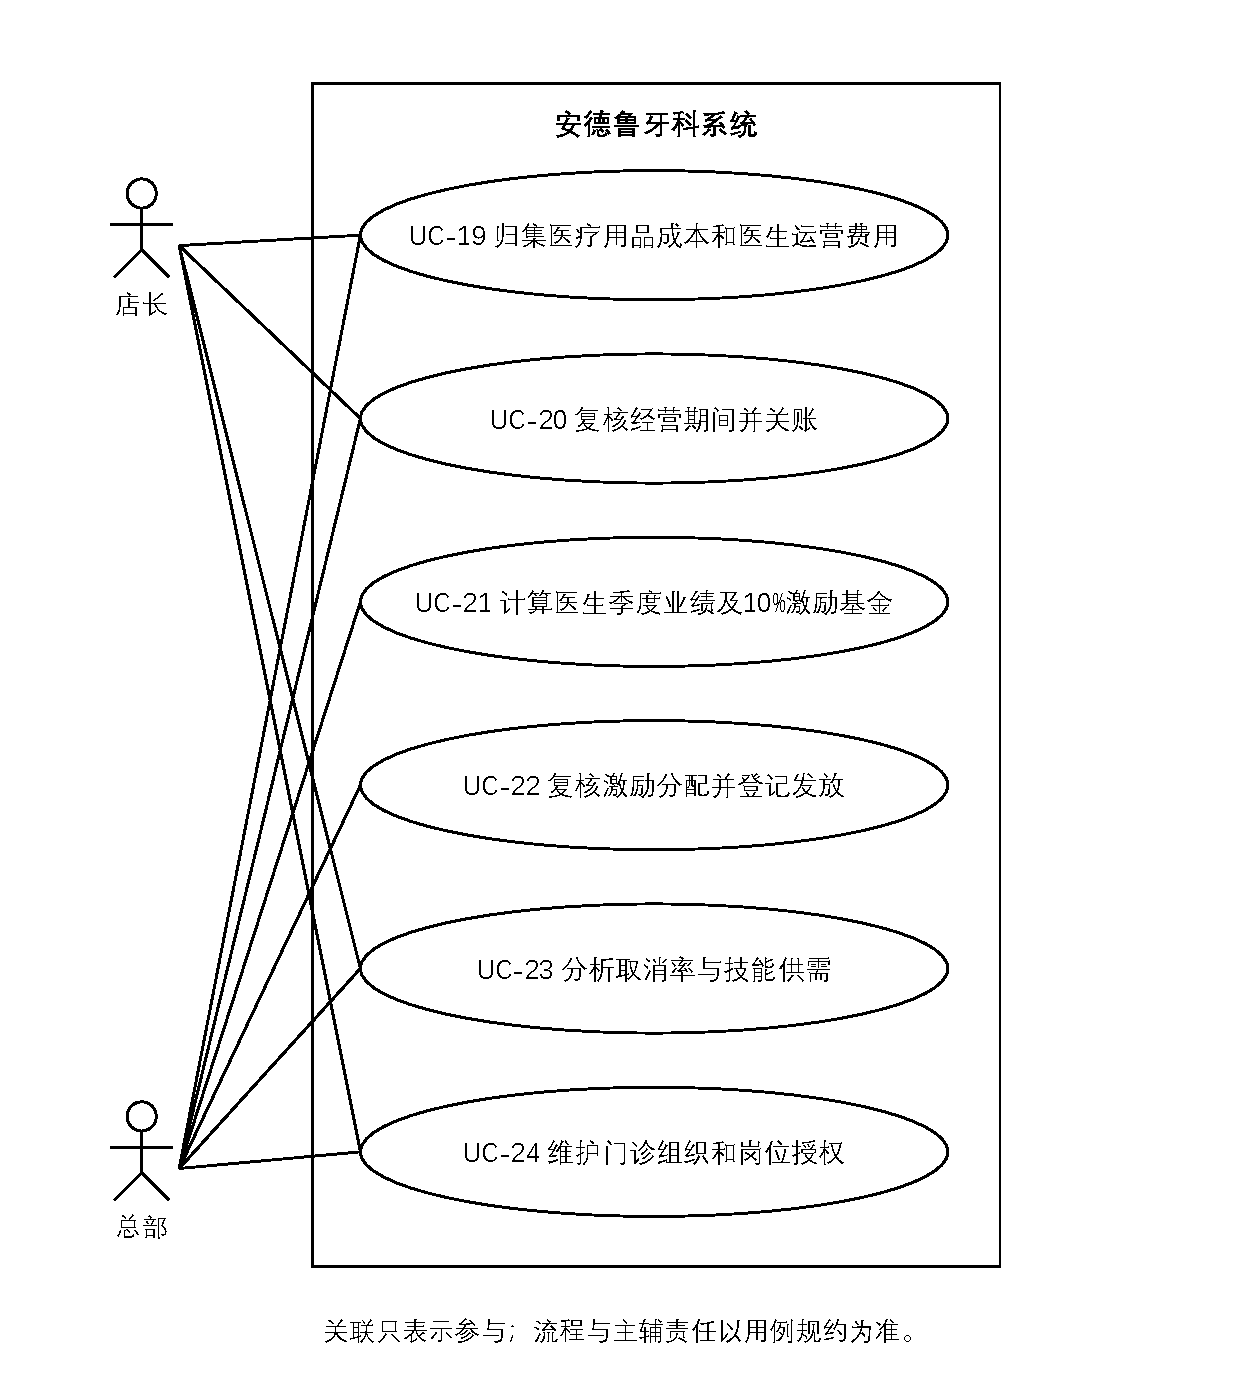
\includegraphics[width=\textwidth]{figures/uc_overview_4.pdf}
\caption{系统用例总览 4}\label{uc_overview_4}\end{figure}
{\fontsize{10.5pt}{13.2pt}\selectfont\setlength{\tabcolsep}{0pt}\renewcommand{\arraystretch}{1.08}
\begin{longtable}{@{}p{1.840cm}@{\hspace{0.16cm}}p{7.640cm}@{\hspace{0.16cm}}p{5.640cm}@{}}
\caption{系统用例索引}\label{tab77}\\
\toprule
\bfseries \Cell{编号} & \bfseries \Cell{目标} & \bfseries \Cell{执行者}\\\midrule
\endfirsthead
\toprule
\bfseries \Cell{编号} & \bfseries \Cell{目标} & \bfseries \Cell{执行者}\\\midrule
\endhead
\bottomrule\endlastfoot
\Cell{\mbox{UC-01}} & \Cell{建立患者档案并核对逐项过敏} & \Cell{顾客、前台、医生}\\[1pt]
\Cell{\mbox{UC-02}} & \Cell{维护牙医档案与专业资格} & \Cell{总部、店长、医生}\\[1pt]
\Cell{\mbox{UC-03}} & \Cell{维护治疗目录与标准单位价格} & \Cell{总部、医生}\\[1pt]
\Cell{\mbox{UC-04}} & \Cell{编排跨店医生班次并发布容量} & \Cell{店长、医生、总部}\\[1pt]
\Cell{\mbox{UC-05}} & \Cell{查询匹配的可预约时段} & \Cell{顾客、前台}\\[1pt]
\Cell{\mbox{UC-06}} & \Cell{确认患者预约} & \Cell{顾客、前台}\\[1pt]
\Cell{\mbox{UC-07}} & \Cell{改期或取消预约} & \Cell{顾客、前台}\\[1pt]
\Cell{\mbox{UC-08}} & \Cell{发送提醒并处理候补邀请} & \Cell{顾客、前台}\\[1pt]
\Cell{\mbox{UC-09}} & \Cell{办理到诊并确认未到情况} & \Cell{前台、医生}\\[1pt]
\Cell{\mbox{UC-10}} & \Cell{接诊检查并制定治疗计划} & \Cell{医生}\\[1pt]
\Cell{\mbox{UC-11}} & \Cell{确认方案及治疗增项} & \Cell{医生、顾客、前台}\\[1pt]
\Cell{\mbox{UC-12}} & \Cell{记录实际治疗与医疗用品耗用} & \Cell{医生}\\[1pt]
\Cell{\mbox{UC-13}} & \Cell{签署病历并追加更正附记} & \Cell{医生}\\[1pt]
\Cell{\mbox{UC-14}} & \Cell{安排复诊及跨店诊疗交接} & \Cell{医生、前台、顾客}\\[1pt]
\Cell{\mbox{UC-15}} & \Cell{生成单次就诊结算单} & \Cell{医生、前台}\\[1pt]
\Cell{\mbox{UC-16}} & \Cell{确认收款并分配到应收} & \Cell{前台、顾客}\\[1pt]
\Cell{\mbox{UC-17}} & \Cell{审批费用更正并办理退款} & \Cell{前台、医生、店长、总部}\\[1pt]
\Cell{\mbox{UC-18}} & \Cell{完成门诊日结及跨店代收核对} & \Cell{前台、店长、总部}\\[1pt]
\Cell{\mbox{UC-19}} & \Cell{归集医疗用品成本和医生运营费用} & \Cell{店长、总部}\\[1pt]
\Cell{\mbox{UC-20}} & \Cell{复核经营期间并关账} & \Cell{总部、店长}\\[1pt]
\Cell{\mbox{UC-21}} & \Cell{计算医生季度业绩及10\%激励基金} & \Cell{总部}\\[1pt]
\Cell{\mbox{UC-22}} & \Cell{复核激励分配并登记发放} & \Cell{总部}\\[1pt]
\Cell{\mbox{UC-23}} & \Cell{分析取消率与技能供需} & \Cell{店长、总部}\\[1pt]
\Cell{\mbox{UC-24}} & \Cell{维护门诊组织和岗位授权} & \Cell{总部、店长}\\[1pt]
\end{longtable}
}
\Needspace{338pt}
\subsection{UC-01 建立患者档案并核对逐项过敏}
\par\noindent\begin{minipage}{\textwidth}
{\fontsize{10.5pt}{13.2pt}\selectfont\setlength{\tabcolsep}{0pt}\renewcommand{\arraystretch}{1.08}
\captionof{table}{UC-01用例约定}\label{tab79}
\begin{tabular}{@{}p{2.440cm}@{\hspace{0.16cm}}p{12.840cm}@{}}
\toprule
\bfseries \Cell{项目} & \bfseries \Cell{内容}\\\midrule
\Cell{执行者} & \Cell{顾客、前台、医生}\\[1pt]
\Cell{触发} & \Cell{患者首次预约或更新联系及过敏资料。}\\[1pt]
\Cell{涉众利益} & \Cell{患者：跨店就诊沿用同一档案，过敏信息不遗漏。\\前台：能处理同名和家庭共用电话，避免串档。\\医生：能区分患者自述、待核实与已核对过敏。}\\[1pt]
\Cell{前置条件} & \Cell{1.\allowbreak{} 办理者为本人、获核实的监护人或有任务权限的员工。\\2.\allowbreak{} 资料收集用途与必要范围已向患者说明。}\\[1pt]
\Cell{成功后置条件} & \Cell{1.\allowbreak{} 生成或沿用唯一患者编号；姓名、出生日期及必要联系资料可查询。\\2.\allowbreak{} 每种已知过敏单独保存，过敏声明及核对人、时间可追溯；疑似重复保持待核对。}\\[1pt]
\bottomrule\end{tabular}
}\end{minipage}\par\vspace{6pt}
\par\noindent\begin{minipage}{\textwidth}
{\fontsize{10.5pt}{13.2pt}\selectfont\setlength{\tabcolsep}{0pt}\renewcommand{\arraystretch}{1.08}
\captionof{table}{UC-01基本与扩展流程}\label{tab80}
\begin{tabular}{@{}p{1.440cm}@{\hspace{0.16cm}}p{13.840cm}@{}}
\toprule
\bfseries \Cell{步骤} & \bfseries \Cell{事件、响应及分支}\\\midrule
\Cell{1} & \Cell{患者或前台填写姓名、出生日期、账单地址、电话和紧急联系人，系统检查必填项与格式。}\\[1pt]
\Cell{2} & \Cell{系统检索可能同人档案，向有权限的办理者显示最小匹配信息；前台核对存在歧义的候选。}\\[1pt]
\Cell{3} & \Cell{患者选择已知过敏、无已知过敏或尚不清楚；存在过敏时逐项选择或补充原述。}\\[1pt]
\Cell{4} & \Cell{系统生成患者编号或沿用核实档案，逐项关联过敏原，保留信息来源。}\\[1pt]
\Cell{5} & \Cell{患者确认联系资料；系统保存确认版本，将未完成医学核对的过敏标为待核实。}\\[1pt]
\Cell{6} & \Cell{医生接诊时复核过敏及反应，系统记录复核结论并保留变更前记录。}\\[1pt]
\Cell{2a} & \Cell{[仅电话相同或存在多个同名候选] 前台进一步核对，不能自动归并；允许保留待核对申请，确认前限制跨档操作。}\\[1pt]
\Cell{3b} & \Cell{[患者无法说明过敏史] 记录未知并向接诊医生提示，不根据空列表生成无过敏结论。}\\[1pt]
\Cell{6c} & \Cell{[患者新报告与既有记录矛盾] 医生登记来源及解释，形成修订记录；原过敏记录保留，不直接删除。}\\[1pt]
\bottomrule\end{tabular}
}\end{minipage}\par\vspace{6pt}
\par\noindent\begin{minipage}{\textwidth}
{\fontsize{10.5pt}{13.2pt}\selectfont\setlength{\tabcolsep}{0pt}\renewcommand{\arraystretch}{1.08}
\captionof{table}{UC-01关键字段}\label{tab81}
\begin{tabular}{@{}p{3.640cm}@{\hspace{0.16cm}}p{5.140cm}@{\hspace{0.16cm}}p{6.340cm}@{}}
\toprule
\bfseries \Cell{字段} & \bfseries \Cell{类型与限制} & \bfseries \Cell{业务含义}\\\midrule
\Cell{患者编号} & \Cell{UUID或稳定业务号，唯一且不可改} & \Cell{关联各店的同一患者}\\[1pt]
\Cell{基本联系} & \Cell{姓名和出生日期必填；电话、账单地址及紧急联系人在正式预约前核实} & \Cell{联系与账单送达}\\[1pt]
\Cell{电子邮箱} & \Cell{可空；合法邮箱格式} & \Cell{患者自愿提供的联系渠道}\\[1pt]
\Cell{过敏声明} & \Cell{known/\allowbreak{}none\_\allowbreak{}reported/\allowbreak{}unknown，必填} & \Cell{区分已知、否认与未知}\\[1pt]
\Cell{过敏条目} & \Cell{过敏原、反应、来源、核对状态；一患者可多条} & \Cell{逐项风险资料}\\[1pt]
\bottomrule\end{tabular}
}\end{minipage}\par\vspace{6pt}
\par\noindent\begin{minipage}{\textwidth}
{\fontsize{10.5pt}{13.2pt}\selectfont\setlength{\tabcolsep}{0pt}\renewcommand{\arraystretch}{1.08}
\captionof{table}{UC-01规则与质量约束}\label{tab82}
\begin{tabular}{@{}p{2.440cm}@{\hspace{0.16cm}}p{12.840cm}@{}}
\toprule
\bfseries \Cell{类别} & \bfseries \Cell{约定}\\\midrule
\Cell{业务规则} & \Cell{1.\allowbreak{} 手机号允许家庭共用，不作患者唯一键。\\2.\allowbreak{} 过敏条目有独立标识；患者自述与医生核对分别记录。\\3.\allowbreak{} 未核实或未知过敏不阻止提出预约意向，治疗前必须由医生确认风险处理。}\\[1pt]
\Cell{质量要求} & \Cell{1.\allowbreak{} 以10万患者为检索验收数据，姓名和出生日期组合查询95\%应在2秒内响应。\\2.\allowbreak{} 越权查询不得返回病历或完整敏感联系资料；新增、修订均有操作记录。}\\[1pt]
\Cell{设计约束} & \Cell{1.\allowbreak{} 患者资料与登录账号分开建模，监护人可代办但不能取代实际患者。\\2.\allowbreak{} 新增过敏原原述进入待整理目录，不由前台判定医学严重程度。}\\[1pt]
\bottomrule\end{tabular}
}\end{minipage}\par\vspace{6pt}
\Needspace{320pt}
\subsection{UC-02 维护牙医档案与专业资格}
\par\noindent\begin{minipage}{\textwidth}
{\fontsize{10.5pt}{13.2pt}\selectfont\setlength{\tabcolsep}{0pt}\renewcommand{\arraystretch}{1.08}
\captionof{table}{UC-02用例约定}\label{tab84}
\begin{tabular}{@{}p{2.440cm}@{\hspace{0.16cm}}p{12.840cm}@{}}
\toprule
\bfseries \Cell{项目} & \bfseries \Cell{内容}\\\midrule
\Cell{执行者} & \Cell{总部、店长、医生}\\[1pt]
\Cell{触发} & \Cell{牙医入职、资料变化、资格核验或证书到期。}\\[1pt]
\Cell{涉众利益} & \Cell{总部：掌握各类专业能力及证书有效期。\\医生：人事资料受控，专业资格与本人对应。\\店长：只能安排满足项目要求的医生。}\\[1pt]
\Cell{前置条件} & \Cell{1.\allowbreak{} 总部维护者有人员或资格核验授权；医生仅提交本人资料。\\2.\allowbreak{} 资格目录已定义名称及可支持的服务范围。}\\[1pt]
\Cell{成功后置条件} & \Cell{1.\allowbreak{} 牙医拥有唯一员工号，必要人事资料与专业资格逐项关联。\\2.\allowbreak{} 资格核验结论、生效范围和时间可查询；失效资格不再支持新增预约。}\\[1pt]
\bottomrule\end{tabular}
}\end{minipage}\par\vspace{6pt}
\par\noindent\begin{minipage}{\textwidth}
{\fontsize{10.5pt}{13.2pt}\selectfont\setlength{\tabcolsep}{0pt}\renewcommand{\arraystretch}{1.08}
\captionof{table}{UC-02基本与扩展流程}\label{tab85}
\begin{tabular}{@{}p{1.440cm}@{\hspace{0.16cm}}p{13.840cm}@{}}
\toprule
\bfseries \Cell{步骤} & \bfseries \Cell{事件、响应及分支}\\\midrule
\Cell{1} & \Cell{总部建立牙医员工号并录入个人资料，系统校验重复员工和必需字段。}\\[1pt]
\Cell{2} & \Cell{医生提交资格名称、证书编号及核验材料，系统关联已有资格目录。}\\[1pt]
\Cell{3} & \Cell{有核验权限的总部人员审查材料，系统记录实际核验人及有效期间。}\\[1pt]
\Cell{4} & \Cell{总部确定可提供的项目及可出诊门诊，系统检查资格与项目要求是否匹配。}\\[1pt]
\Cell{5} & \Cell{系统保存获核实资格及授权；店长查询有效技能清单，失效或待核实项明确区分。}\\[1pt]
\Cell{6} & \Cell{资格终止或范围缩小时，系统列出受影响班次及预约，由店长协调后续安排。}\\[1pt]
\Cell{2a} & \Cell{[资格名称尚未进入目录] 总部审核并建立目录项后再关联；自由文本证书不自动取得项目资格。}\\[1pt]
\Cell{3b} & \Cell{[材料不足或核验未通过] 保存待补或退回原因，资格保持不可用于新增安排。}\\[1pt]
\Cell{6c} & \Cell{[已有预约超出新的资格有效范围] 生成逐项协调任务，保留原承诺和处置记录，不静默删除预约。}\\[1pt]
\bottomrule\end{tabular}
}\end{minipage}\par\vspace{6pt}
\par\noindent\begin{minipage}{\textwidth}
{\fontsize{10.5pt}{13.2pt}\selectfont\setlength{\tabcolsep}{0pt}\renewcommand{\arraystretch}{1.08}
\captionof{table}{UC-02关键字段}\label{tab86}
\begin{tabular}{@{}p{3.640cm}@{\hspace{0.16cm}}p{5.140cm}@{\hspace{0.16cm}}p{6.340cm}@{}}
\toprule
\bfseries \Cell{字段} & \bfseries \Cell{类型与限制} & \bfseries \Cell{业务含义}\\\midrule
\Cell{员工号} & \Cell{稳定唯一业务号，必填} & \Cell{跨店识别同一牙医}\\[1pt]
\Cell{人事资料} & \Cell{姓名、出生日期、家庭住址、电话、邮箱} & \Cell{供人员管理与必要联系}\\[1pt]
\Cell{专业资格} & \Cell{目录编号及证书编号；一牙医可多项} & \Cell{表达技能组合}\\[1pt]
\Cell{资格状态} & \Cell{pending/\allowbreak{}verified/\allowbreak{}expired/\allowbreak{}revoked} & \Cell{约束出诊安排}\\[1pt]
\Cell{核验范围} & \Cell{适用项目、门诊、有效期间及核验人} & \Cell{支持可预约能力检查}\\[1pt]
\bottomrule\end{tabular}
}\end{minipage}\par\vspace{6pt}
\par\noindent\begin{minipage}{\textwidth}
{\fontsize{10.5pt}{13.2pt}\selectfont\setlength{\tabcolsep}{0pt}\renewcommand{\arraystretch}{1.08}
\captionof{table}{UC-02规则与质量约束}\label{tab87}
\begin{tabular}{@{}p{2.440cm}@{\hspace{0.16cm}}p{12.840cm}@{}}
\toprule
\bfseries \Cell{类别} & \bfseries \Cell{约定}\\\midrule
\Cell{业务规则} & \Cell{1.\allowbreak{} 员工号不因跨店出诊改变。\\2.\allowbreak{} 牙医与专业资格为多对多关系，不能只存一个职称字符串。\\3.\allowbreak{} 项目能力授权依赖有效资格；运营管理身份不授予诊疗签署权。}\\[1pt]
\Cell{质量要求} & \Cell{1.\allowbreak{} 验收将一项资格置为失效后，所有新号源查询均排除不合资格的安排。\\2.\allowbreak{} 普通预约查询只展示姓名、专长和可出诊信息，不返回住址与出生日期。}\\[1pt]
\Cell{设计约束} & \Cell{1.\allowbreak{} 证书有效期依核验资料录入，无明确截止日时保留其依据，不虚构到期日。\\2.\allowbreak{} 人事档案变更、资格核验及项目授权分别留操作记录。}\\[1pt]
\bottomrule\end{tabular}
}\end{minipage}\par\vspace{6pt}
\Needspace{320pt}
\subsection{UC-03 维护治疗目录与标准单位价格}
\par\noindent\begin{minipage}{\textwidth}
{\fontsize{10.5pt}{13.2pt}\selectfont\setlength{\tabcolsep}{0pt}\renewcommand{\arraystretch}{1.08}
\captionof{table}{UC-03用例约定}\label{tab89}
\begin{tabular}{@{}p{2.440cm}@{\hspace{0.16cm}}p{12.840cm}@{}}
\toprule
\bfseries \Cell{项目} & \bfseries \Cell{内容}\\\midrule
\Cell{执行者} & \Cell{总部、医生}\\[1pt]
\Cell{触发} & \Cell{新增治疗项目或调整标准单位、价格及适用条件。}\\[1pt]
\Cell{涉众利益} & \Cell{患者：能了解项目及其计价单位。\\医生：实际记录有统一项目和单位。\\总部：各门店使用可追溯的标准价格。}\\[1pt]
\Cell{前置条件} & \Cell{1.\allowbreak{} 维护者具有总部服务标准授权。\\2.\allowbreak{} 项目内容及所需技能由有专业责任的医生确认。}\\[1pt]
\Cell{成功后置条件} & \Cell{1.\allowbreak{} 生成明确生效期间的治疗项目及价格版本。\\2.\allowbreak{} 历史计划、执行和账单保留其使用的单位与价格，不随目录调整改变。}\\[1pt]
\bottomrule\end{tabular}
}\end{minipage}\par\vspace{6pt}
\par\noindent\begin{minipage}{\textwidth}
{\fontsize{10.5pt}{13.2pt}\selectfont\setlength{\tabcolsep}{0pt}\renewcommand{\arraystretch}{1.08}
\captionof{table}{UC-03基本与扩展流程}\label{tab90}
\begin{tabular}{@{}p{1.440cm}@{\hspace{0.16cm}}p{13.840cm}@{}}
\toprule
\bfseries \Cell{步骤} & \bfseries \Cell{事件、响应及分支}\\\midrule
\Cell{1} & \Cell{总部提出治疗名称、项目编码及计价单位，系统检查同义或重复项目。}\\[1pt]
\Cell{2} & \Cell{医生确认服务内容、适用技能和建议预约时长，系统保存专业确认。}\\[1pt]
\Cell{3} & \Cell{总部录入标准单位价格及生效日期，系统检查金额精度和时间范围。}\\[1pt]
\Cell{4} & \Cell{系统展示与现行版本的差异及受影响的未确认方案，维护者确认发布。}\\[1pt]
\Cell{5} & \Cell{系统建立新价格版本并更新可用目录，未来选价按业务日期匹配。}\\[1pt]
\Cell{6} & \Cell{医生或前台查询项目，系统返回名称、单位、适用价及需评估后确定的限制。}\\[1pt]
\Cell{1a} & \Cell{[拟建项目与已有编码重复] 返回已有项目供核对，不再建立另一个同义编码。}\\[1pt]
\Cell{3b} & \Cell{[生效期间与同范围价格重叠] 拒绝发布，要求明确旧版截止点和新版起点。}\\[1pt]
\Cell{5c} & \Cell{[旧版本已被执行或账单引用] 保留旧版；停用只影响新业务，不覆盖历史快照。}\\[1pt]
\bottomrule\end{tabular}
}\end{minipage}\par\vspace{6pt}
\par\noindent\begin{minipage}{\textwidth}
{\fontsize{10.5pt}{13.2pt}\selectfont\setlength{\tabcolsep}{0pt}\renewcommand{\arraystretch}{1.08}
\captionof{table}{UC-03关键字段}\label{tab91}
\begin{tabular}{@{}p{3.640cm}@{\hspace{0.16cm}}p{5.140cm}@{\hspace{0.16cm}}p{6.340cm}@{}}
\toprule
\bfseries \Cell{字段} & \bfseries \Cell{类型与限制} & \bfseries \Cell{业务含义}\\\midrule
\Cell{项目编码} & \Cell{唯一且稳定，TEXT} & \Cell{统一统计治疗类别}\\[1pt]
\Cell{项目名称及内容} & \Cell{必填，保留历史描述} & \Cell{解释实际服务}\\[1pt]
\Cell{标准单位} & \Cell{必填，如次、牙或约定标准单位} & \Cell{数量与单价的共同尺度}\\[1pt]
\Cell{标准单价} & \Cell{非负整数分} & \Cell{每标准单位的价格}\\[1pt]
\Cell{适用条件} & \Cell{技能要求、时长及生效起止} & \Cell{支撑预约与计价}\\[1pt]
\bottomrule\end{tabular}
}\end{minipage}\par\vspace{6pt}
\par\noindent\begin{minipage}{\textwidth}
{\fontsize{10.5pt}{13.2pt}\selectfont\setlength{\tabcolsep}{0pt}\renewcommand{\arraystretch}{1.08}
\captionof{table}{UC-03规则与质量约束}\label{tab92}
\begin{tabular}{@{}p{2.440cm}@{\hspace{0.16cm}}p{12.840cm}@{}}
\toprule
\bfseries \Cell{类别} & \bfseries \Cell{约定}\\\midrule
\Cell{业务规则} & \Cell{1.\allowbreak{} 治疗数量允许按项目规定的小数精度记录，禁止浮点金额运算。\\2.\allowbreak{} 同项目同适用范围同一时点只能匹配一个有效价目版本。\\3.\allowbreak{} 医生记录实际数量和适用单价依据，正式账单从执行及确认价格形成。}\\[1pt]
\Cell{质量要求} & \Cell{1.\allowbreak{} 修改目录价格后复算历史账单，原金额应保持不变。\\2.\allowbreak{} 价目发布须能追到发布人及版本；未授权账号写入应被拒绝。}\\[1pt]
\Cell{设计约束} & \Cell{1.\allowbreak{} 估计费用与实际费用分别展示；复杂主诉不能仅依据目录自动诊断。\\2.\allowbreak{} 计价单位改变时建立新版本，不能在已有数量上直接替换单位。}\\[1pt]
\bottomrule\end{tabular}
}\end{minipage}\par\vspace{6pt}
\Needspace{320pt}
\subsection{UC-04 编排跨店医生班次并发布容量}
\par\noindent\begin{minipage}{\textwidth}
{\fontsize{10.5pt}{13.2pt}\selectfont\setlength{\tabcolsep}{0pt}\renewcommand{\arraystretch}{1.08}
\captionof{table}{UC-04用例约定}\label{tab94}
\begin{tabular}{@{}p{2.440cm}@{\hspace{0.16cm}}p{12.840cm}@{}}
\toprule
\bfseries \Cell{项目} & \bfseries \Cell{内容}\\\midrule
\Cell{执行者} & \Cell{店长、医生、总部}\\[1pt]
\Cell{触发} & \Cell{门店编排出诊周期或调整医生班次。}\\[1pt]
\Cell{涉众利益} & \Cell{患者：预约得到可以履行的医生和时间。\\医生：跨店出诊不冲突，并留出转场条件。\\店长：了解本店技能供给与实际容量。}\\[1pt]
\Cell{前置条件} & \Cell{1.\allowbreak{} 门诊正常运营，地址及营业时间已维护。\\2.\allowbreak{} 排班者有门诊范围授权，医生资格及项目目录可查询。}\\[1pt]
\Cell{成功后置条件} & \Cell{1.\allowbreak{} 仅符合有效资格、营业及跨店约束的班次发布为可预约容量。\\2.\allowbreak{} 已预约时段不被静默覆盖，受影响预约有协调任务。}\\[1pt]
\bottomrule\end{tabular}
}\end{minipage}\par\vspace{6pt}
\par\noindent\begin{minipage}{\textwidth}
{\fontsize{10.5pt}{13.2pt}\selectfont\setlength{\tabcolsep}{0pt}\renewcommand{\arraystretch}{1.08}
\captionof{table}{UC-04基本与扩展流程}\label{tab95}
\begin{tabular}{@{}p{1.440cm}@{\hspace{0.16cm}}p{13.840cm}@{}}
\toprule
\bfseries \Cell{步骤} & \bfseries \Cell{事件、响应及分支}\\\midrule
\Cell{1} & \Cell{店长选择门诊及周期，系统显示营业安排、已占用时段和可用医生技能。}\\[1pt]
\Cell{2} & \Cell{医生或店长提出跨店班次，系统读取该医生全部门诊班次。}\\[1pt]
\Cell{3} & \Cell{系统检查时间重叠和转场缓冲，并核对班次内项目资格有效期。}\\[1pt]
\Cell{4} & \Cell{店长结合本店治疗位和服务时长确认容量，系统检查资源可用条件。}\\[1pt]
\Cell{5} & \Cell{系统展示排班结果及受影响预约，店长对可履行安排确认发布。}\\[1pt]
\Cell{6} & \Cell{系统保存班次版本并开放号源；调整涉及旧预约时，前台收到逐人协调任务。}\\[1pt]
\Cell{3a} & \Cell{[医生在另一门诊已有重叠班次或转场时间不足] 指出冲突门诊及时间，不发布；由相关店长与医生协商。}\\[1pt]
\Cell{4b} & \Cell{[资格将在班次期间失效或治疗位停用] 限制可发布的项目或时段，不能以总部权限代替专业资格。}\\[1pt]
\Cell{5c} & \Cell{[缩减容量影响已确认预约] 保留原承诺，先提出替诊或改约安排，确认处理后再发布对应变更。}\\[1pt]
\bottomrule\end{tabular}
}\end{minipage}\par\vspace{6pt}
\par\noindent\begin{minipage}{\textwidth}
{\fontsize{10.5pt}{13.2pt}\selectfont\setlength{\tabcolsep}{0pt}\renewcommand{\arraystretch}{1.08}
\captionof{table}{UC-04关键字段}\label{tab96}
\begin{tabular}{@{}p{3.640cm}@{\hspace{0.16cm}}p{5.140cm}@{\hspace{0.16cm}}p{6.340cm}@{}}
\toprule
\bfseries \Cell{字段} & \bfseries \Cell{类型与限制} & \bfseries \Cell{业务含义}\\\midrule
\Cell{班次编号} & \Cell{UUID；医生和门诊外键必填} & \Cell{标识一次出诊安排}\\[1pt]
\Cell{起止时间} & \Cell{带时区时间，起点小于终点} & \Cell{采用半开区间判断占用}\\[1pt]
\Cell{可提供项目} & \Cell{有效资格覆盖的项目集合} & \Cell{保证技能匹配}\\[1pt]
\Cell{资源容量} & \Cell{治疗位及可接诊时长} & \Cell{限制可承诺预约}\\[1pt]
\Cell{转场缓冲} & \Cell{非负分钟及规则版本} & \Cell{约束不同地点连续班次}\\[1pt]
\bottomrule\end{tabular}
}\end{minipage}\par\vspace{6pt}
\par\noindent\begin{minipage}{\textwidth}
{\fontsize{10.5pt}{13.2pt}\selectfont\setlength{\tabcolsep}{0pt}\renewcommand{\arraystretch}{1.08}
\captionof{table}{UC-04规则与质量约束}\label{tab97}
\begin{tabular}{@{}p{2.440cm}@{\hspace{0.16cm}}p{12.840cm}@{}}
\toprule
\bfseries \Cell{类别} & \bfseries \Cell{约定}\\\midrule
\Cell{业务规则} & \Cell{1.\allowbreak{} 全连锁同一医生不能同时在两处出诊。\\2.\allowbreak{} 转场缓冲由组织配置并可说明依据，不把不同门诊视为同一地点。\\3.\allowbreak{} 发布前再次检查已有预约和资格，查询通过不替代提交时校验。}\\[1pt]
\Cell{质量要求} & \Cell{1.\allowbreak{} 以30门诊100牙医的排班数据验收，跨店冲突扫描95\%应在3秒内给出结果。\\2.\allowbreak{} 并发发布重叠班次时，数据库约束或提交锁应保证最多一个成功。}\\[1pt]
\Cell{设计约束} & \Cell{1.\allowbreak{} 店长仅维护授权门诊，总部处理跨店协调授权；排班不改变医生专业资格。\\2.\allowbreak{} 冻结或停诊需要保存原因及原版本。}\\[1pt]
\bottomrule\end{tabular}
}\end{minipage}\par\vspace{6pt}
\Needspace{338pt}
\subsection{UC-05 查询匹配的可预约时段}
\par\noindent\begin{minipage}{\textwidth}
{\fontsize{10.5pt}{13.2pt}\selectfont\setlength{\tabcolsep}{0pt}\renewcommand{\arraystretch}{1.08}
\captionof{table}{UC-05用例约定}\label{tab99}
\begin{tabular}{@{}p{2.440cm}@{\hspace{0.16cm}}p{12.840cm}@{}}
\toprule
\bfseries \Cell{项目} & \bfseries \Cell{内容}\\\midrule
\Cell{执行者} & \Cell{顾客、前台}\\[1pt]
\Cell{触发} & \Cell{患者选择治疗诉求、门诊偏好和时间范围。}\\[1pt]
\Cell{涉众利益} & \Cell{患者：按治疗诉求找到适合的门诊与牙医。\\前台：代约与线上查询使用同一容量。\\医生：接诊项目与技能及时长相符。}\\[1pt]
\Cell{前置条件} & \Cell{1.\allowbreak{} 存在已发布班次及有效服务目录。\\2.\allowbreak{} 查询范围不包含应隐藏的人员信息。}\\[1pt]
\Cell{成功后置条件} & \Cell{1.\allowbreak{} 返回符合门诊、技能、连续时长及资源条件的候选时段，标注价格估计及适用限制。\\2.\allowbreak{} 查询不占用资源；无合适时段时明确返回空结果和可用替代条件。}\\[1pt]
\bottomrule\end{tabular}
}\end{minipage}\par\vspace{6pt}
\par\noindent\begin{minipage}{\textwidth}
{\fontsize{10.5pt}{13.2pt}\selectfont\setlength{\tabcolsep}{0pt}\renewcommand{\arraystretch}{1.08}
\captionof{table}{UC-05基本与扩展流程}\label{tab100}
\begin{tabular}{@{}p{1.440cm}@{\hspace{0.16cm}}p{13.840cm}@{}}
\toprule
\bfseries \Cell{步骤} & \bfseries \Cell{事件、响应及分支}\\\midrule
\Cell{1} & \Cell{患者或前台输入项目、日期及门诊偏好，系统解释需要先检查的主诉类别。}\\[1pt]
\Cell{2} & \Cell{系统匹配项目所需资格和建议时长，过滤未获准线上直接预约的项目。}\\[1pt]
\Cell{3} & \Cell{系统检索符合技能的跨店班次，并核对服务日期上的资格。}\\[1pt]
\Cell{4} & \Cell{系统从班次内扣除已确认预约、有效暂占和停用资源，查找连续可容纳时段。}\\[1pt]
\Cell{5} & \Cell{系统按患者选择的地点和时间展示候选，说明治疗估价、医生及确认条件。}\\[1pt]
\Cell{6} & \Cell{患者选择一个候选，系统带入确认页并重新读取状态，提示最终预约以确认结果为准。}\\[1pt]
\Cell{2a} & \Cell{[主诉需要医生评估，无法安全确定项目时长] 返回初诊检查或人工协调入口，不自动把症状转为确定诊断。}\\[1pt]
\Cell{4b} & \Cell{[没有匹配时段] 显示原因及扩大日期、门诊范围或登记候补的选项，不显示虚假空闲。}\\[1pt]
\Cell{6c} & \Cell{[候选在浏览期间已被占用] 刷新候选并说明变化，尚未形成预约无需取消旧单。}\\[1pt]
\bottomrule\end{tabular}
}\end{minipage}\par\vspace{6pt}
\par\noindent\begin{minipage}{\textwidth}
{\fontsize{10.5pt}{13.2pt}\selectfont\setlength{\tabcolsep}{0pt}\renewcommand{\arraystretch}{1.08}
\captionof{table}{UC-05关键字段}\label{tab101}
\begin{tabular}{@{}p{3.640cm}@{\hspace{0.16cm}}p{5.140cm}@{\hspace{0.16cm}}p{6.340cm}@{}}
\toprule
\bfseries \Cell{字段} & \bfseries \Cell{类型与限制} & \bfseries \Cell{业务含义}\\\midrule
\Cell{项目或主诉} & \Cell{项目编号或有限长度原述} & \Cell{区分明确项目与待评估诉求}\\[1pt]
\Cell{期望范围} & \Cell{门诊集合、日期区间与医生偏好} & \Cell{限制查询及展示}\\[1pt]
\Cell{连续时长} & \Cell{正整数分钟，源自服务规则} & \Cell{保证一次安排能容纳服务}\\[1pt]
\Cell{候选时段} & \Cell{医生、门诊、起止、资源版本及查询时间} & \Cell{只代表查询时的可用性}\\[1pt]
\Cell{费用估计} & \Cell{标准单位和参考单价，注明非最终账单} & \Cell{帮助患者理解费用边界}\\[1pt]
\bottomrule\end{tabular}
}\end{minipage}\par\vspace{6pt}
\par\noindent\begin{minipage}{\textwidth}
{\fontsize{10.5pt}{13.2pt}\selectfont\setlength{\tabcolsep}{0pt}\renewcommand{\arraystretch}{1.08}
\captionof{table}{UC-05规则与质量约束}\label{tab102}
\begin{tabular}{@{}p{2.440cm}@{\hspace{0.16cm}}p{12.840cm}@{}}
\toprule
\bfseries \Cell{类别} & \bfseries \Cell{约定}\\\midrule
\Cell{业务规则} & \Cell{1.\allowbreak{} 不同门诊的同一医生共用全局占用检查。\\2.\allowbreak{} 查询结果不构成号源保留，也不保证主诉对应的最终治疗。\\3.\allowbreak{} 默认按时间和偏好排序，不能仅按项目收费高低推荐。}\\[1pt]
\Cell{质量要求} & \Cell{1.\allowbreak{} 在30门诊100牙医、近90天排班的验收集上，50并发查询95\%应在2秒内返回。\\2.\allowbreak{} 候选查询结果不含其他患者姓名、联系方式或诊疗信息。}\\[1pt]
\Cell{设计约束} & \Cell{1.\allowbreak{} 使用分页与限定日期范围；界面以门诊当地时间展示。\\2.\allowbreak{} 前台代约读取同一查询服务，不维护离线独立号源。}\\[1pt]
\bottomrule\end{tabular}
}\end{minipage}\par\vspace{6pt}
\Needspace{338pt}
\subsection{UC-06 确认患者预约}
\par\noindent\begin{minipage}{\textwidth}
{\fontsize{10.5pt}{13.2pt}\selectfont\setlength{\tabcolsep}{0pt}\renewcommand{\arraystretch}{1.08}
\captionof{table}{UC-06用例约定}\label{tab104}
\begin{tabular}{@{}p{2.440cm}@{\hspace{0.16cm}}p{12.840cm}@{}}
\toprule
\bfseries \Cell{项目} & \bfseries \Cell{内容}\\\midrule
\Cell{执行者} & \Cell{顾客、前台}\\[1pt]
\Cell{触发} & \Cell{患者选中候选时段并提交预约确认。}\\[1pt]
\Cell{涉众利益} & \Cell{患者：获得明确日期、地点和牙医的有效预约。\\门店：避免线上与电话代约重复占用。\\医生：接诊任务及患者诉求可预先查询。}\\[1pt]
\Cell{前置条件} & \Cell{1.\allowbreak{} 实际患者主档已确定，必要联系资料可核实；过敏未知有明确声明。\\2.\allowbreak{} 时段对应已发布班次，办理者有本人或代约权限。}\\[1pt]
\Cell{成功后置条件} & \Cell{1.\allowbreak{} 生成唯一预约号，关联患者、门诊、牙医和实际占用；初始到诊标记为false。\\2.\allowbreak{} 重复提交返回同一结果；确认失败不留下永久占用。}\\[1pt]
\bottomrule\end{tabular}
}\end{minipage}\par\vspace{6pt}
\par\noindent\begin{minipage}{\textwidth}
{\fontsize{10.5pt}{13.2pt}\selectfont\setlength{\tabcolsep}{0pt}\renewcommand{\arraystretch}{1.08}
\captionof{table}{UC-06基本与扩展流程}\label{tab105}
\begin{tabular}{@{}p{1.440cm}@{\hspace{0.16cm}}p{13.840cm}@{}}
\toprule
\bfseries \Cell{步骤} & \bfseries \Cell{事件、响应及分支}\\\midrule
\Cell{1} & \Cell{患者或前台核对实际患者、就诊诉求与所选时段，系统展示到诊要求及取消规则。}\\[1pt]
\Cell{2} & \Cell{系统建立短时确认暂占，向办理者显示截止时间；暂占只保留同一次确认所需资源。}\\[1pt]
\Cell{3} & \Cell{患者确认联系资料和规则，前台代约时记录患者同意及来电诉求。}\\[1pt]
\Cell{4} & \Cell{系统在提交时重新检查资格、班次、时长和资源，确认该暂占仍有效。}\\[1pt]
\Cell{5} & \Cell{系统以同一事务建立预约及资源占用，撤销相应暂占并生成确认回执。}\\[1pt]
\Cell{6} & \Cell{系统向患者返回预约号及准确地点时间，随后登记提醒任务；发送失败进入前台待办。}\\[1pt]
\Cell{2a} & \Cell{[资源已被其他请求占用] 返回冲突及最新候选，尚未成功的请求不得显示预约成立。}\\[1pt]
\Cell{4b} & \Cell{[暂占到期或资格、班次已变更] 释放无效暂占并重新查询；保留本次输入以便重选。}\\[1pt]
\Cell{5c} & \Cell{[同一确认请求因网络重试重复提交] 按幂等键返回原预约及回执，不创建第二张预约单。}\\[1pt]
\Cell{6d} & \Cell{[通知发送失败] 预约保持有效，生成联系任务，不因通知失败重新占号。}\\[1pt]
\bottomrule\end{tabular}
}\end{minipage}\par\vspace{6pt}
\par\noindent\begin{minipage}{\textwidth}
{\fontsize{10.5pt}{13.2pt}\selectfont\setlength{\tabcolsep}{0pt}\renewcommand{\arraystretch}{1.08}
\captionof{table}{UC-06关键字段}\label{tab106}
\begin{tabular}{@{}p{3.640cm}@{\hspace{0.16cm}}p{5.140cm}@{\hspace{0.16cm}}p{6.340cm}@{}}
\toprule
\bfseries \Cell{字段} & \bfseries \Cell{类型与限制} & \bfseries \Cell{业务含义}\\\midrule
\Cell{预约号} & \Cell{全连锁唯一稳定业务号} & \Cell{查询及到店核对}\\[1pt]
\Cell{患者及接诊方} & \Cell{患者、牙医、门诊外键均必填} & \Cell{明确服务双方与地点}\\[1pt]
\Cell{时段与诉求} & \Cell{开始、结束、项目或主诉原述} & \Cell{确定服务承诺}\\[1pt]
\Cell{暂占} & \Cell{截止时刻及资源版本} & \Cell{控制确认期间竞争}\\[1pt]
\Cell{幂等键} & \Cell{同一确认意图唯一} & \Cell{处理重复点击和网络重试}\\[1pt]
\Cell{出席标记} & \Cell{BOOLEAN，初始false} & \Cell{独立保留实际到诊事实}\\[1pt]
\bottomrule\end{tabular}
}\end{minipage}\par\vspace{6pt}
\par\noindent\begin{minipage}{\textwidth}
{\fontsize{10.5pt}{13.2pt}\selectfont\setlength{\tabcolsep}{0pt}\renewcommand{\arraystretch}{1.08}
\captionof{table}{UC-06规则与质量约束}\label{tab107}
\begin{tabular}{@{}p{2.440cm}@{\hspace{0.16cm}}p{12.840cm}@{}}
\toprule
\bfseries \Cell{类别} & \bfseries \Cell{约定}\\\midrule
\Cell{业务规则} & \Cell{1.\allowbreak{} 预约确认不等同到诊或完成治疗。\\2.\allowbreak{} 同一医生和治疗资源的有效占用不得重叠。\\3.\allowbreak{} 暂占时长按已公布规则配置，到期不再保障资源。}\\[1pt]
\Cell{质量要求} & \Cell{1.\allowbreak{} 以50个并发确认同一时段验收，最多一个有效预约成功，其他请求有明确结果。\\2.\allowbreak{} 返回成功前应已持久化预约及占用；服务重启后可凭预约号查询。}\\[1pt]
\Cell{设计约束} & \Cell{1.\allowbreak{} 预约确认暂不以预付款为必需条件；费用估计不生成治疗收入。\\2.\allowbreak{} 提醒异步执行，预约与通知各有状态。}\\[1pt]
\bottomrule\end{tabular}
}\end{minipage}\par\vspace{6pt}
\Needspace{320pt}
\subsection{UC-07 改期或取消预约}
\par\noindent\begin{minipage}{\textwidth}
{\fontsize{10.5pt}{13.2pt}\selectfont\setlength{\tabcolsep}{0pt}\renewcommand{\arraystretch}{1.08}
\captionof{table}{UC-07用例约定}\label{tab109}
\begin{tabular}{@{}p{2.440cm}@{\hspace{0.16cm}}p{12.840cm}@{}}
\toprule
\bfseries \Cell{项目} & \bfseries \Cell{内容}\\\midrule
\Cell{执行者} & \Cell{顾客、前台}\\[1pt]
\Cell{触发} & \Cell{患者提出更改日期、地点或取消已确认预约。}\\[1pt]
\Cell{涉众利益} & \Cell{患者：改约失败时保有原有安排，取消有明确回执。\\门店：释放的时段能再次安排，取消原因可分析。\\医生：出诊任务变更及时可见。}\\[1pt]
\Cell{前置条件} & \Cell{1.\allowbreak{} 预约属于本人或办理者的授权任务，尚未开始实际接诊。\\2.\allowbreak{} 原预约及变更规则可查询；改期已选择候选新时段。}\\[1pt]
\Cell{成功后置条件} & \Cell{1.\allowbreak{} 成功改期时新旧预约关联且只有新资源有效；取消时保留原记录和原因。\\2.\allowbreak{} 失败不破坏原预约；操作有经办人、时间和可查询回执。}\\[1pt]
\bottomrule\end{tabular}
}\end{minipage}\par\vspace{6pt}
\par\noindent\begin{minipage}{\textwidth}
{\fontsize{10.5pt}{13.2pt}\selectfont\setlength{\tabcolsep}{0pt}\renewcommand{\arraystretch}{1.08}
\captionof{table}{UC-07基本与扩展流程}\label{tab110}
\begin{tabular}{@{}p{1.440cm}@{\hspace{0.16cm}}p{13.840cm}@{}}
\toprule
\bfseries \Cell{步骤} & \bfseries \Cell{事件、响应及分支}\\\midrule
\Cell{1} & \Cell{患者或前台选中原预约并说明变更意图，系统展示当前状态及适用规则。}\\[1pt]
\Cell{2} & \Cell{改期者选择新时段，系统尝试取得必要暂占；取消者确认取消原因。}\\[1pt]
\Cell{3} & \Cell{系统检查办理权限、原预约版本及自助变更窗口，临近就诊的例外交前台协调。}\\[1pt]
\Cell{4} & \Cell{办理者确认影响；系统在提交时检查原预约仍可变更，并重新校验新时段。}\\[1pt]
\Cell{5} & \Cell{改期一次提交新预约关联与资源替换；取消追加取消事件并释放原占用，原到诊事实不被改写。}\\[1pt]
\Cell{6} & \Cell{系统返回回执并登记医生及患者通知；释放时段交候补匹配，相关费用争议另行受理。}\\[1pt]
\Cell{2a} & \Cell{[新时段竞争失败或暂占到期] 保留原预约和占用，返回可选时段，不先取消旧约。}\\[1pt]
\Cell{3b} & \Cell{[超出自助变更窗口] 转前台核实患者诉求及接诊影响，未经确认不自动取消。}\\[1pt]
\Cell{4c} & \Cell{[原预约已开始接诊或被他人改动] 拒绝当前变更并刷新状态；实际服务及账务问题进入对应处理流程。}\\[1pt]
\bottomrule\end{tabular}
}\end{minipage}\par\vspace{6pt}
\par\noindent\begin{minipage}{\textwidth}
{\fontsize{10.5pt}{13.2pt}\selectfont\setlength{\tabcolsep}{0pt}\renewcommand{\arraystretch}{1.08}
\captionof{table}{UC-07关键字段}\label{tab111}
\begin{tabular}{@{}p{3.640cm}@{\hspace{0.16cm}}p{5.140cm}@{\hspace{0.16cm}}p{6.340cm}@{}}
\toprule
\bfseries \Cell{字段} & \bfseries \Cell{类型与限制} & \bfseries \Cell{业务含义}\\\midrule
\Cell{变更类型} & \Cell{reschedule/\allowbreak{}cancel，必填} & \Cell{决定替换资源或解除占用}\\[1pt]
\Cell{原预约版本} & \Cell{预约号与版本，必填} & \Cell{避免覆盖他人变更}\\[1pt]
\Cell{新安排} & \Cell{改期时必填新班次及起止} & \Cell{明确新的服务承诺}\\[1pt]
\Cell{原因及经办人} & \Cell{原因分类、原述、实际操作账号} & \Cell{分析取消且可追溯}\\[1pt]
\Cell{变更关联} & \Cell{旧预约号、新预约号及事件号} & \Cell{避免改期两次计入取消}\\[1pt]
\bottomrule\end{tabular}
}\end{minipage}\par\vspace{6pt}
\par\noindent\begin{minipage}{\textwidth}
{\fontsize{10.5pt}{13.2pt}\selectfont\setlength{\tabcolsep}{0pt}\renewcommand{\arraystretch}{1.08}
\captionof{table}{UC-07规则与质量约束}\label{tab112}
\begin{tabular}{@{}p{2.440cm}@{\hspace{0.16cm}}p{12.840cm}@{}}
\toprule
\bfseries \Cell{类别} & \bfseries \Cell{约定}\\\midrule
\Cell{业务规则} & \Cell{1.\allowbreak{} 改期失败必须保留旧约，改期成功不能出现双占。\\2.\allowbreak{} 取消、改期和未到分开记录；患者取消与医生停诊原因分开。\\3.\allowbreak{} 取消预约不直接等同退款，实际收退由资金用例核验。}\\[1pt]
\Cell{质量要求} & \Cell{1.\allowbreak{} 以两个并发变更请求验收，只接受与当前版本一致的一次，其他请求返回新状态。\\2.\allowbreak{} 网络重试不重复释放资源或生成多张改期预约。}\\[1pt]
\Cell{设计约束} & \Cell{1.\allowbreak{} 已发生的到诊和治疗不通过取消预约删除。\\2.\allowbreak{} 保留时间与取消窗口由统一政策配置，界面在操作前展示。}\\[1pt]
\bottomrule\end{tabular}
}\end{minipage}\par\vspace{6pt}
\Needspace{338pt}
\subsection{UC-08 发送提醒并处理候补邀请}
\par\noindent\begin{minipage}{\textwidth}
{\fontsize{10.5pt}{13.2pt}\selectfont\setlength{\tabcolsep}{0pt}\renewcommand{\arraystretch}{1.08}
\captionof{table}{UC-08用例约定}\label{tab114}
\begin{tabular}{@{}p{2.440cm}@{\hspace{0.16cm}}p{12.840cm}@{}}
\toprule
\bfseries \Cell{项目} & \bfseries \Cell{内容}\\\midrule
\Cell{执行者} & \Cell{顾客、前台}\\[1pt]
\Cell{触发} & \Cell{达到预约提醒时点，或有可预约空档释放。}\\[1pt]
\Cell{涉众利益} & \Cell{患者：及时收到到诊提示，并可选择适合的候补空档。\\前台：通知失败与未回应者有明确待办。\\门店：释放空档按适配条件利用，避免超额承诺。}\\[1pt]
\Cell{前置条件} & \Cell{1.\allowbreak{} 患者有有效联系渠道及接收偏好。\\2.\allowbreak{} 提醒关联有效预约；候补有患者意愿、时间及项目条件。}\\[1pt]
\Cell{成功后置条件} & \Cell{1.\allowbreak{} 每次提醒或邀请有发送、送达、回应等分开状态。\\2.\allowbreak{} 候补邀请有截止时间；接受者仍通过预约确认竞争资源，未接受不形成预约。}\\[1pt]
\bottomrule\end{tabular}
}\end{minipage}\par\vspace{6pt}
\par\noindent\begin{minipage}{\textwidth}
{\fontsize{10.5pt}{13.2pt}\selectfont\setlength{\tabcolsep}{0pt}\renewcommand{\arraystretch}{1.08}
\captionof{table}{UC-08基本与扩展流程}\label{tab115}
\begin{tabular}{@{}p{1.440cm}@{\hspace{0.16cm}}p{13.840cm}@{}}
\toprule
\bfseries \Cell{步骤} & \bfseries \Cell{事件、响应及分支}\\\midrule
\Cell{1} & \Cell{系统依据有效预约和提醒规则列出待提醒者，前台可检查联系人及特殊说明。}\\[1pt]
\Cell{2} & \Cell{空档释放时，系统匹配候补的门诊、项目、时长及患者可用时间，排除已撤回需求。}\\[1pt]
\Cell{3} & \Cell{系统建立提醒或限时邀请任务，记录内容版本和接收偏好；同一触发不重复建立任务。}\\[1pt]
\Cell{4} & \Cell{发送适配器投递消息，系统保存受理及投递结果；前台处理失败渠道或改为人工联系。}\\[1pt]
\Cell{5} & \Cell{患者查看消息并回应；普通提醒记录确认，候补接受进入预约确认，拒绝或超时保留原因。}\\[1pt]
\Cell{6} & \Cell{系统依据最终预约结果关闭已满足需求或恢复可候补状态，并向前台显示未解决事项。}\\[1pt]
\Cell{2a} & \Cell{[没有满足条件的候补患者] 空档仍公开可约，不为填满时段降低技能或时长要求。}\\[1pt]
\Cell{4b} & \Cell{[发送失败或联系方式无效] 保留任务及失败原因，交前台核对；不得把受理状态记为送达。}\\[1pt]
\Cell{5c} & \Cell{[多人接受同一空档或邀请已过期] 确认时重新检查资源；未成功者保留原预约和候补意愿，不显示补位成功。}\\[1pt]
\bottomrule\end{tabular}
}\end{minipage}\par\vspace{6pt}
\par\noindent\begin{minipage}{\textwidth}
{\fontsize{10.5pt}{13.2pt}\selectfont\setlength{\tabcolsep}{0pt}\renewcommand{\arraystretch}{1.08}
\captionof{table}{UC-08关键字段}\label{tab116}
\begin{tabular}{@{}p{3.640cm}@{\hspace{0.16cm}}p{5.140cm}@{\hspace{0.16cm}}p{6.340cm}@{}}
\toprule
\bfseries \Cell{字段} & \bfseries \Cell{类型与限制} & \bfseries \Cell{业务含义}\\\midrule
\Cell{候补条件} & \Cell{患者、项目、门诊范围和可用时间} & \Cell{确定兼容空档}\\[1pt]
\Cell{消息任务} & \Cell{类型、关联预约或空档、内容版本} & \Cell{解释本次联系目的}\\[1pt]
\Cell{投递状态} & \Cell{pending/\allowbreak{}sent/\allowbreak{}delivered/\allowbreak{}failed} & \Cell{区分发送与实际送达}\\[1pt]
\Cell{回应状态} & \Cell{accepted/\allowbreak{}declined/\allowbreak{}expired/\allowbreak{}no\_\allowbreak{}response} & \Cell{区分意愿和业务成立}\\[1pt]
\Cell{邀请截止} & \Cell{明确时间且晚于创建时间} & \Cell{限制失效邀请继续使用}\\[1pt]
\bottomrule\end{tabular}
}\end{minipage}\par\vspace{6pt}
\par\noindent\begin{minipage}{\textwidth}
{\fontsize{10.5pt}{13.2pt}\selectfont\setlength{\tabcolsep}{0pt}\renewcommand{\arraystretch}{1.08}
\captionof{table}{UC-08规则与质量约束}\label{tab117}
\begin{tabular}{@{}p{2.440cm}@{\hspace{0.16cm}}p{12.840cm}@{}}
\toprule
\bfseries \Cell{类别} & \bfseries \Cell{约定}\\\midrule
\Cell{业务规则} & \Cell{1.\allowbreak{} 候补邀请不等于正式预约，接受后引用\mbox{UC-06}确认。\\2.\allowbreak{} 已有预约的提前候补成功时，原约替换通过\mbox{UC-07}处理。\\3.\allowbreak{} 不在普通提醒中发送详细病情；尊重患者渠道偏好。}\\[1pt]
\Cell{质量要求} & \Cell{1.\allowbreak{} 重复触发同一预约提醒事件时，只生成一项有效任务。\\2.\allowbreak{} 模拟消息服务超时，预约与候补记录保持可查询，失败任务可恢复。}\\[1pt]
\Cell{设计约束} & \Cell{1.\allowbreak{} 通知服务调用在业务提交后执行；重试复用同一任务标识。\\2.\allowbreak{} 人工电话联系也登记结果，不能伪造电子送达。}\\[1pt]
\bottomrule\end{tabular}
}\end{minipage}\par\vspace{6pt}
\Needspace{320pt}
\subsection{UC-09 办理到诊并确认未到情况}
\par\noindent\begin{minipage}{\textwidth}
{\fontsize{10.5pt}{13.2pt}\selectfont\setlength{\tabcolsep}{0pt}\renewcommand{\arraystretch}{1.08}
\captionof{table}{UC-09用例约定}\label{tab119}
\begin{tabular}{@{}p{2.440cm}@{\hspace{0.16cm}}p{12.840cm}@{}}
\toprule
\bfseries \Cell{项目} & \bfseries \Cell{内容}\\\midrule
\Cell{执行者} & \Cell{前台、医生}\\[1pt]
\Cell{触发} & \Cell{患者到店，或预约达到未到核实时点。}\\[1pt]
\Cell{涉众利益} & \Cell{患者：真实到诊被识别，迟到有合理协调。\\前台：能核对预约与实际到店情况。\\总部：取消与未到的指标有可靠事实。}\\[1pt]
\Cell{前置条件} & \Cell{1.\allowbreak{} 办理者有本门诊接待权限，原预约和患者身份可查。\\2.\allowbreak{} 未到处理规则已定义核实时间、联系步骤及资源释放条件。}\\[1pt]
\Cell{成功后置条件} & \Cell{1.\allowbreak{} 实际到诊者创建一次就诊并更新到诊事实；同预约不能重复创建有效就诊。\\2.\allowbreak{} 未到结论有核实记录，预约取消与未到分开；未满足条件不释放资源。}\\[1pt]
\bottomrule\end{tabular}
}\end{minipage}\par\vspace{6pt}
\par\noindent\begin{minipage}{\textwidth}
{\fontsize{10.5pt}{13.2pt}\selectfont\setlength{\tabcolsep}{0pt}\renewcommand{\arraystretch}{1.08}
\captionof{table}{UC-09基本与扩展流程}\label{tab120}
\begin{tabular}{@{}p{1.440cm}@{\hspace{0.16cm}}p{13.840cm}@{}}
\toprule
\bfseries \Cell{步骤} & \bfseries \Cell{事件、响应及分支}\\\midrule
\Cell{1} & \Cell{前台按预约号或最小身份信息找到患者，系统显示门诊、时段和原状态。}\\[1pt]
\Cell{2} & \Cell{到店者由前台核实身份及到达时间；尚未到店者登记联系结果，系统保留核实依据。}\\[1pt]
\Cell{3} & \Cell{系统检查重复签到、已取消及已接诊状态，提示需要纠正的矛盾。}\\[1pt]
\Cell{4} & \Cell{确认实际到诊时，系统创建就诊号，将预约到诊标记更新为true并登记实际时间。}\\[1pt]
\Cell{5} & \Cell{仍未到者由前台按规则判断是否已满足未到条件；系统记录no\_\allowbreak{}show，保持到诊标记false并按条件释放资源。}\\[1pt]
\Cell{6} & \Cell{系统返回候诊交接或未到处理结果；迟到需缩减或改约时交医生判断可安全接诊范围。}\\[1pt]
\Cell{2a} & \Cell{[联系不上且尚未达到处理时点] 保留待核实状态及原占用，安排再次核实，不能提前判未到。}\\[1pt]
\Cell{3b} & \Cell{[患者已到但存在漏签到或错误取消] 核对实际证据，由有权人员追加更正事件，不删除原记录。}\\[1pt]
\Cell{4c} & \Cell{[重复签到请求] 返回已有就诊号，不创建第二次同预约就诊。}\\[1pt]
\bottomrule\end{tabular}
}\end{minipage}\par\vspace{6pt}
\par\noindent\begin{minipage}{\textwidth}
{\fontsize{10.5pt}{13.2pt}\selectfont\setlength{\tabcolsep}{0pt}\renewcommand{\arraystretch}{1.08}
\captionof{table}{UC-09关键字段}\label{tab121}
\begin{tabular}{@{}p{3.640cm}@{\hspace{0.16cm}}p{5.140cm}@{\hspace{0.16cm}}p{6.340cm}@{}}
\toprule
\bfseries \Cell{字段} & \bfseries \Cell{类型与限制} & \bfseries \Cell{业务含义}\\\midrule
\Cell{到诊标记} & \Cell{BOOLEAN，预约初始false} & \Cell{只表达实际出席}\\[1pt]
\Cell{到达时间} & \Cell{实际时间，不能晚于已记录接诊而无说明} & \Cell{计算等候及核实出席}\\[1pt]
\Cell{未到结论} & \Cell{pending/\allowbreak{}no\_\allowbreak{}show及原因、联系结果} & \Cell{区分未核实与已认定}\\[1pt]
\Cell{就诊号} & \Cell{唯一，关联患者、门诊和预约} & \Cell{承载一次实际服务}\\[1pt]
\Cell{核实记录} & \Cell{经办人、时点、依据、原新状态} & \Cell{支持纠错和统计}\\[1pt]
\bottomrule\end{tabular}
}\end{minipage}\par\vspace{6pt}
\par\noindent\begin{minipage}{\textwidth}
{\fontsize{10.5pt}{13.2pt}\selectfont\setlength{\tabcolsep}{0pt}\renewcommand{\arraystretch}{1.08}
\captionof{table}{UC-09规则与质量约束}\label{tab122}
\begin{tabular}{@{}p{2.440cm}@{\hspace{0.16cm}}p{12.840cm}@{}}
\toprule
\bfseries \Cell{类别} & \bfseries \Cell{约定}\\\midrule
\Cell{业务规则} & \Cell{1.\allowbreak{} 到诊false包括尚未来到等情况，不能直接用作取消数量。\\2.\allowbreak{} 确认到诊、医疗开始和治疗完成分别记录。\\3.\allowbreak{} 只有已满足规则的未到结论才允许释放对应资源。}\\[1pt]
\Cell{质量要求} & \Cell{1.\allowbreak{} 连续或并发重复签到应返回同一就诊号。\\2.\allowbreak{} 取消、改期、未到与到诊的汇总可逐条回查原事件，不允许无依据改总数。}\\[1pt]
\Cell{设计约束} & \Cell{1.\allowbreak{} 不能用自动时间阈值替代实际到诊核实。\\2.\allowbreak{} 漏签到纠正保留前后状态及责任人，统计使用有效更正后的事实。}\\[1pt]
\bottomrule\end{tabular}
}\end{minipage}\par\vspace{6pt}
\Needspace{338pt}
\subsection{UC-10 接诊检查并制定治疗计划}
\par\noindent\begin{minipage}{\textwidth}
{\fontsize{10.5pt}{13.2pt}\selectfont\setlength{\tabcolsep}{0pt}\renewcommand{\arraystretch}{1.08}
\captionof{table}{UC-10用例约定}\label{tab124}
\begin{tabular}{@{}p{2.440cm}@{\hspace{0.16cm}}p{12.840cm}@{}}
\toprule
\bfseries \Cell{项目} & \bfseries \Cell{内容}\\\midrule
\Cell{执行者} & \Cell{医生}\\[1pt]
\Cell{触发} & \Cell{医生接收已到诊患者并开始检查。}\\[1pt]
\Cell{涉众利益} & \Cell{患者：检查结论与特殊需求得到连续记录。\\医生：保留诊断判断并取得完整风险资料。\\其他门诊接诊医生：可查已有诊断及尚未完成的计划。}\\[1pt]
\Cell{前置条件} & \Cell{1.\allowbreak{} 存在实际就诊号，医生对该次就诊有接诊权限及有效资格。\\2.\allowbreak{} 患者身份、过敏声明和历史资料可核对。}\\[1pt]
\Cell{成功后置条件} & \Cell{1.\allowbreak{} 诊断、特殊需求及医生处理意见与本次就诊关联。\\2.\allowbreak{} 形成有版本的治疗计划草案，含项目、顺序及费用估计；未确认草案不直接放行治疗。}\\[1pt]
\bottomrule\end{tabular}
}\end{minipage}\par\vspace{6pt}
\par\noindent\begin{minipage}{\textwidth}
{\fontsize{10.5pt}{13.2pt}\selectfont\setlength{\tabcolsep}{0pt}\renewcommand{\arraystretch}{1.08}
\captionof{table}{UC-10基本与扩展流程}\label{tab125}
\begin{tabular}{@{}p{1.440cm}@{\hspace{0.16cm}}p{13.840cm}@{}}
\toprule
\bfseries \Cell{步骤} & \bfseries \Cell{事件、响应及分支}\\\midrule
\Cell{1} & \Cell{医生选择本次就诊，系统核对患者、门诊和接诊权限，显示跨店必要历史。}\\[1pt]
\Cell{2} & \Cell{医生逐项核对过敏及本次特殊需求，系统记录核实来源与需处理的风险。}\\[1pt]
\Cell{3} & \Cell{医生完成检查并录入诊断、牙位和处置判断，系统检查结构化字段完整性。}\\[1pt]
\Cell{4} & \Cell{医生拟定一项或多项治疗，系统关联标准单位、价格版本和项目所需技能。}\\[1pt]
\Cell{5} & \Cell{存在分次治疗时，医生确定阶段顺序、间隔及复评条件，系统检查依赖是否形成循环。}\\[1pt]
\Cell{6} & \Cell{系统保存计划草案及估价，供医生向患者解释；复杂风险未解决时记录暂缓或转诊意见。}\\[1pt]
\Cell{2a} & \Cell{[过敏史矛盾或风险尚不能判断] 医生补问并记录处理意见；尚不具备安全条件时只保留检查结论，不放行相关治疗。}\\[1pt]
\Cell{4b} & \Cell{[拟治疗超出当前医生或门诊能力] 记录需要的技能，安排其他合格医生或门诊评估，不能仅靠运营授权继续。}\\[1pt]
\Cell{5c} & \Cell{[阶段相互依赖或日期条件不合理] 指出循环或冲突，修订后才能形成可执行计划。}\\[1pt]
\bottomrule\end{tabular}
}\end{minipage}\par\vspace{6pt}
\par\noindent\begin{minipage}{\textwidth}
{\fontsize{10.5pt}{13.2pt}\selectfont\setlength{\tabcolsep}{0pt}\renewcommand{\arraystretch}{1.08}
\captionof{table}{UC-10关键字段}\label{tab126}
\begin{tabular}{@{}p{3.640cm}@{\hspace{0.16cm}}p{5.140cm}@{\hspace{0.16cm}}p{6.340cm}@{}}
\toprule
\bfseries \Cell{字段} & \bfseries \Cell{类型与限制} & \bfseries \Cell{业务含义}\\\midrule
\Cell{诊断记录} & \Cell{诊断原述、牙位、医生及检查时间} & \Cell{表达医学判断}\\[1pt]
\Cell{特殊需求} & \Cell{患者问题及医生回应，保留来源} & \Cell{支持连续照护}\\[1pt]
\Cell{计划版本} & \Cell{患者、责任医生、版本号及草案状态} & \Cell{区分修订内容}\\[1pt]
\Cell{阶段及条件} & \Cell{前置阶段、间隔和复评要求} & \Cell{约束后续安排}\\[1pt]
\Cell{计划项目} & \Cell{治疗、标准单位、估计数量及适用单价} & \Cell{形成费用估计}\\[1pt]
\bottomrule\end{tabular}
}\end{minipage}\par\vspace{6pt}
\par\noindent\begin{minipage}{\textwidth}
{\fontsize{10.5pt}{13.2pt}\selectfont\setlength{\tabcolsep}{0pt}\renewcommand{\arraystretch}{1.08}
\captionof{table}{UC-10规则与质量约束}\label{tab127}
\begin{tabular}{@{}p{2.440cm}@{\hspace{0.16cm}}p{12.840cm}@{}}
\toprule
\bfseries \Cell{类别} & \bfseries \Cell{约定}\\\midrule
\Cell{业务规则} & \Cell{1.\allowbreak{} 诊断和治疗先后由医生确定，系统不根据症状自动下诊断。\\2.\allowbreak{} 阶段未完成不等于整份计划失败，后续就诊可以继续同一计划。\\3.\allowbreak{} 计划估计数量与实际执行数量分别记录。}\\[1pt]
\Cell{质量要求} & \Cell{1.\allowbreak{} 跨店历史查询按本次接诊任务授权；撤销接诊权限后应拒绝新增读取。\\2.\allowbreak{} 验收构造阶段循环依赖时，系统应拒绝将该版本设为可执行。}\\[1pt]
\Cell{设计约束} & \Cell{1.\allowbreak{} 签署后的诊断更正保留原文，追加有原因及签名的附记。\\2.\allowbreak{} 计划必须进入\mbox{UC-11}确认，保存草案本身不产生收费和已完成事实。}\\[1pt]
\bottomrule\end{tabular}
}\end{minipage}\par\vspace{6pt}
\Needspace{320pt}
\subsection{UC-11 确认方案及治疗增项}
\par\noindent\begin{minipage}{\textwidth}
{\fontsize{10.5pt}{13.2pt}\selectfont\setlength{\tabcolsep}{0pt}\renewcommand{\arraystretch}{1.08}
\captionof{table}{UC-11用例约定}\label{tab129}
\begin{tabular}{@{}p{2.440cm}@{\hspace{0.16cm}}p{12.840cm}@{}}
\toprule
\bfseries \Cell{项目} & \bfseries \Cell{内容}\\\midrule
\Cell{执行者} & \Cell{医生、顾客、前台}\\[1pt]
\Cell{触发} & \Cell{医生准备实施计划，或就诊中发现需增加、替换治疗。}\\[1pt]
\Cell{涉众利益} & \Cell{患者：理解治疗内容、费用与替代选择，有权拒绝或暂缓。\\医生：实际执行范围与已说明内容一致。\\前台：只能依据确认范围安排后续与结算。}\\[1pt]
\Cell{前置条件} & \Cell{1.\allowbreak{} 有明确版本的计划或增项草案，解释者具备对应专业责任。\\2.\allowbreak{} 实际患者或经核实监护人可确认，必要时提供适合的解释方式。}\\[1pt]
\Cell{成功后置条件} & \Cell{1.\allowbreak{} 接受、拒绝或暂缓均有独立记录，签认绑定确切版本和费用范围。\\2.\allowbreak{} 新增或替换项目只有取得相应确认后才进入可执行范围，旧确认不被覆盖。}\\[1pt]
\bottomrule\end{tabular}
}\end{minipage}\par\vspace{6pt}
\par\noindent\begin{minipage}{\textwidth}
{\fontsize{10.5pt}{13.2pt}\selectfont\setlength{\tabcolsep}{0pt}\renewcommand{\arraystretch}{1.08}
\captionof{table}{UC-11基本与扩展流程}\label{tab130}
\begin{tabular}{@{}p{1.440cm}@{\hspace{0.16cm}}p{13.840cm}@{}}
\toprule
\bfseries \Cell{步骤} & \bfseries \Cell{事件、响应及分支}\\\midrule
\Cell{1} & \Cell{医生选择待确认方案或提出增项，系统列出治疗名称、单位、估计数量、单价与变更原因。}\\[1pt]
\Cell{2} & \Cell{医生向患者解释目的、顺序、风险及可选择方案，前台可协助说明费用安排。}\\[1pt]
\Cell{3} & \Cell{系统展示本次与原版本的差异和总价影响，患者提出疑问后由相应责任人回答。}\\[1pt]
\Cell{4} & \Cell{患者明确接受、拒绝或暂缓，系统核对确认人身份、代办关系及签认对象。}\\[1pt]
\Cell{5} & \Cell{接受时系统保存具体版本、说明及确认凭据，拒绝或暂缓时记录范围和原因。}\\[1pt]
\Cell{6} & \Cell{系统返回可执行项目及未获同意部分；后续执行只引用有效确认范围。}\\[1pt]
\Cell{3a} & \Cell{[患者认为费用或增项内容不清楚] 返回医生或费用说明，形成修订版后重新确认，不能默认接受。}\\[1pt]
\Cell{4b} & \Cell{[确认人不能证明适格身份或监护关系] 保留待确认，不用手机号相同推定签认资格。}\\[1pt]
\Cell{5c} & \Cell{[患者拒绝或暂缓部分项目] 记录未接受范围，医生调整后续方案；系统不得把部分接受变为整份全选。}\\[1pt]
\bottomrule\end{tabular}
}\end{minipage}\par\vspace{6pt}
\par\noindent\begin{minipage}{\textwidth}
{\fontsize{10.5pt}{13.2pt}\selectfont\setlength{\tabcolsep}{0pt}\renewcommand{\arraystretch}{1.08}
\captionof{table}{UC-11关键字段}\label{tab131}
\begin{tabular}{@{}p{3.640cm}@{\hspace{0.16cm}}p{5.140cm}@{\hspace{0.16cm}}p{6.340cm}@{}}
\toprule
\bfseries \Cell{字段} & \bfseries \Cell{类型与限制} & \bfseries \Cell{业务含义}\\\midrule
\Cell{确认对象} & \Cell{计划版本及明确项目集合} & \Cell{固定患者同意范围}\\[1pt]
\Cell{增项理由} & \Cell{诊疗发现、替换原因及医生} & \Cell{解释实际变更}\\[1pt]
\Cell{费用快照} & \Cell{单位、数量、单价及估计总额} & \Cell{保证说明可复现}\\[1pt]
\Cell{确认人} & \Cell{患者或有效监护人及核实依据} & \Cell{明确签认责任}\\[1pt]
\Cell{确认结论} & \Cell{accepted/\allowbreak{}declined/\allowbreak{}deferred；时间及凭据} & \Cell{区别同意、拒绝和暂缓}\\[1pt]
\bottomrule\end{tabular}
}\end{minipage}\par\vspace{6pt}
\par\noindent\begin{minipage}{\textwidth}
{\fontsize{10.5pt}{13.2pt}\selectfont\setlength{\tabcolsep}{0pt}\renewcommand{\arraystretch}{1.08}
\captionof{table}{UC-11规则与质量约束}\label{tab132}
\begin{tabular}{@{}p{2.440cm}@{\hspace{0.16cm}}p{12.840cm}@{}}
\toprule
\bfseries \Cell{类别} & \bfseries \Cell{约定}\\\midrule
\Cell{业务规则} & \Cell{1.\allowbreak{} 患者确认之前不得将增项写成已执行治疗。\\2.\allowbreak{} 实质内容、价格范围或治疗阶段改变时重新说明并确认。\\3.\allowbreak{} 前台可解释账务，但不能替代医生作诊断或医疗风险说明。}\\[1pt]
\Cell{质量要求} & \Cell{1.\allowbreak{} 调取任一已确认版本应能复现当时项目及费用范围，后续改价不得改写。\\2.\allowbreak{} 重复提交同一签认请求应产生同一确认编号。}\\[1pt]
\Cell{设计约束} & \Cell{1.\allowbreak{} 电子确认机制需保留可核对身份、时间及内容摘要；线下签认保存受控凭据引用。\\2.\allowbreak{} 医疗紧急例外依据专业判断记录原因及处置，不能由预约或收费权限自动豁免。}\\[1pt]
\bottomrule\end{tabular}
}\end{minipage}\par\vspace{6pt}
\Needspace{355pt}
\subsection{UC-12 记录实际治疗与医疗用品耗用}
\par\noindent\begin{minipage}{\textwidth}
{\fontsize{10.5pt}{13.2pt}\selectfont\setlength{\tabcolsep}{0pt}\renewcommand{\arraystretch}{1.08}
\captionof{table}{UC-12用例约定}\label{tab134}
\begin{tabular}{@{}p{2.440cm}@{\hspace{0.16cm}}p{12.840cm}@{}}
\toprule
\bfseries \Cell{项目} & \bfseries \Cell{内容}\\\midrule
\Cell{执行者} & \Cell{医生}\\[1pt]
\Cell{触发} & \Cell{医生实施或结束本次治疗，并记录实际项目与用品。}\\[1pt]
\Cell{涉众利益} & \Cell{患者：实际治疗和收费依据一致，未做项目不冒充完成。\\医生：记录实际工作及用品消耗，跨店贡献可核算。\\总部：医疗用品成本能追到医生、就诊与用品来源。}\\[1pt]
\Cell{前置条件} & \Cell{1.\allowbreak{} 存在本次实际就诊，医生资格、过敏处理及适用确认条件已满足。\\2.\allowbreak{} 项目有明确标准单位和适用价目版本，用品计量单位可识别。}\\[1pt]
\Cell{成功后置条件} & \Cell{1.\allowbreak{} 每项实际治疗保存操作者、数量、标准单位及单价快照；完成、中止及未做明确区分。\\2.\allowbreak{} 用品实际耗用关联治疗、医生及门诊；缺成本证据进入待归集，不虚填零成本。}\\[1pt]
\bottomrule\end{tabular}
}\end{minipage}\par\vspace{6pt}
\par\noindent\begin{minipage}{\textwidth}
{\fontsize{10.5pt}{13.2pt}\selectfont\setlength{\tabcolsep}{0pt}\renewcommand{\arraystretch}{1.08}
\captionof{table}{UC-12基本与扩展流程}\label{tab135}
\begin{tabular}{@{}p{1.440cm}@{\hspace{0.16cm}}p{13.840cm}@{}}
\toprule
\bfseries \Cell{步骤} & \bfseries \Cell{事件、响应及分支}\\\midrule
\Cell{1} & \Cell{医生选取本次可执行项目，系统核对确认版本、阶段条件及医生有效资格。}\\[1pt]
\Cell{2} & \Cell{医生实施治疗并登记牙位、实际标准单位数量和完成情况，系统显示适用单位与价格依据。}\\[1pt]
\Cell{3} & \Cell{治疗增加或替换项目时，系统引导先完成\mbox{UC-11}说明确认，再允许记录相应执行。}\\[1pt]
\Cell{4} & \Cell{医生记录实际使用的医疗用品、数量及可识别批次或来源，系统检查计量单位和重复记录。}\\[1pt]
\Cell{5} & \Cell{系统展示本次治疗与耗用清单，医生核对并签署实际事实；部分完成注明范围与原因。}\\[1pt]
\Cell{6} & \Cell{系统保存执行及耗用关联，向结算单提供本次已完成治疗明细，向成本归集提供待计价用品事实。}\\[1pt]
\Cell{1a} & \Cell{[确认版本失效、阶段前置未完成或资格不符] 相关治疗不放行；医生复评或取得有效确认，不能由前台修改状态绕过。}\\[1pt]
\Cell{4b} & \Cell{[用品实际已用但成本或来源资料尚不完整] 如实记录数量和待补原因，交成本归集处理；不得虚构采购价。}\\[1pt]
\Cell{5c} & \Cell{[治疗中止或只完成部分标准单位] 按实际数量和完成范围保存，未做部分不形成已完成收费依据。}\\[1pt]
\Cell{6d} & \Cell{[签署后发现记录错误] 追加有原因、时间和医生签名的更正，原事实保留；账务影响另经结算调整。}\\[1pt]
\bottomrule\end{tabular}
}\end{minipage}\par\vspace{6pt}
\par\noindent\begin{minipage}{\textwidth}
{\fontsize{10.5pt}{13.2pt}\selectfont\setlength{\tabcolsep}{0pt}\renewcommand{\arraystretch}{1.08}
\captionof{table}{UC-12关键字段}\label{tab136}
\begin{tabular}{@{}p{3.640cm}@{\hspace{0.16cm}}p{5.140cm}@{\hspace{0.16cm}}p{6.340cm}@{}}
\toprule
\bfseries \Cell{字段} & \bfseries \Cell{类型与限制} & \bfseries \Cell{业务含义}\\\midrule
\Cell{治疗执行} & \Cell{就诊、治疗项目、牙位、医生及时间} & \Cell{确定实际服务事实}\\[1pt]
\Cell{计价快照} & \Cell{标准单位、实际数量、单价分及价格版本} & \Cell{结算逐行可复算}\\[1pt]
\Cell{完成情况} & \Cell{completed/\allowbreak{}partial/\allowbreak{}not\_\allowbreak{}performed及原因} & \Cell{区别计划和履约}\\[1pt]
\Cell{用品耗用} & \Cell{用品、数量、计量单位、来源及责任医生} & \Cell{支持直接成本归属}\\[1pt]
\Cell{签署凭据} & \Cell{签署人、时间、内容摘要及更正关联} & \Cell{保持已签事实不可覆盖}\\[1pt]
\bottomrule\end{tabular}
}\end{minipage}\par\vspace{6pt}
\par\noindent\begin{minipage}{\textwidth}
{\fontsize{10.5pt}{13.2pt}\selectfont\setlength{\tabcolsep}{0pt}\renewcommand{\arraystretch}{1.08}
\captionof{table}{UC-12规则与质量约束}\label{tab137}
\begin{tabular}{@{}p{2.440cm}@{\hspace{0.16cm}}p{12.840cm}@{}}
\toprule
\bfseries \Cell{类别} & \bfseries \Cell{约定}\\\midrule
\Cell{业务规则} & \Cell{1.\allowbreak{} 一次就诊可有多项实际治疗，后续汇成同一张该次就诊结算单。\\2.\allowbreak{} 每项操作保留实际执行医生，不能全部归到预约指定医生。\\3.\allowbreak{} 用品成本按实际耗用归属，不把采购付款直接当本次医生成本。}\\[1pt]
\Cell{质量要求} & \Cell{1.\allowbreak{} 原执行与签署内容应可复现；更正后可同时查看原文及有效差异。\\2.\allowbreak{} 重复提交签署请求不得重复生成治疗或用品耗用记录。}\\[1pt]
\Cell{设计约束} & \Cell{1.\allowbreak{} 数量用定点小数，金额用整数分；标准单位快照与实际单价不得只依赖当前目录。\\2.\allowbreak{} 系统承载记录与规则检查，临床判断由医生负责。}\\[1pt]
\bottomrule\end{tabular}
}\end{minipage}\par\vspace{6pt}
\Needspace{320pt}
\subsection{UC-13 签署病历并追加更正附记}
\par\noindent\begin{minipage}{\textwidth}
{\fontsize{10.5pt}{13.2pt}\selectfont\setlength{\tabcolsep}{0pt}\renewcommand{\arraystretch}{1.08}
\captionof{table}{UC-13用例约定}\label{tab139}
\begin{tabular}{@{}p{2.440cm}@{\hspace{0.16cm}}p{12.840cm}@{}}
\toprule
\bfseries \Cell{项目} & \bfseries \Cell{内容}\\\midrule
\Cell{执行者} & \Cell{医生}\\[1pt]
\Cell{触发} & \Cell{医生结束本次处置后提交病历签署，或发现已签署记录需要更正。}\\[1pt]
\Cell{涉众利益} & \Cell{顾客：诊疗记录准确，后续接诊可理解既往处置\\医生：签署责任清楚，错误可更正且历史不被覆盖\\店长：查明记录缺漏并督促原医生处理}\\[1pt]
\Cell{前置条件} & \Cell{1.\allowbreak{} 就诊属于该医生负责或已授权接续的诊疗任务；患者身份已核对。\\2.\allowbreak{} 待签草稿记录本次检查、诊断和实际处置；存在当前版本号。}\\[1pt]
\Cell{成功后置条件} & \Cell{1.\allowbreak{} 签署版本、医生身份、签署时间及内容摘要一并保存。\\2.\allowbreak{} 更正形成引用原签署版本的新附记；原文及历次附记可按时间查阅。}\\[1pt]
\bottomrule\end{tabular}
}\end{minipage}\par\vspace{6pt}
\par\noindent\begin{minipage}{\textwidth}
{\fontsize{10.5pt}{13.2pt}\selectfont\setlength{\tabcolsep}{0pt}\renewcommand{\arraystretch}{1.08}
\captionof{table}{UC-13基本与扩展流程}\label{tab140}
\begin{tabular}{@{}p{1.440cm}@{\hspace{0.16cm}}p{13.840cm}@{}}
\toprule
\bfseries \Cell{步骤} & \bfseries \Cell{事件、响应及分支}\\\midrule
\Cell{1} & \Cell{医生打开本次就诊记录，系统显示草稿、实际执行项目及未完成事项。}\\[1pt]
\Cell{2} & \Cell{医生核对诊断、牙位、处置及医嘱，补齐必填项后提交签署。}\\[1pt]
\Cell{3} & \Cell{系统检查医生权限、草稿版本和实际执行关联，展示待签内容。}\\[1pt]
\Cell{4} & \Cell{医生确认签署；系统保存不可覆盖的签署版本并锁定相应草稿。}\\[1pt]
\Cell{5} & \Cell{医生发现错误时选择原记录，填写更正原因、正确内容及受影响事项。}\\[1pt]
\Cell{6} & \Cell{系统显示原文与附记对照；医生确认后签署附记。}\\[1pt]
\Cell{7} & \Cell{系统追加附记并通知有后续接诊任务的医生；涉及收费差异时生成费用核对任务。}\\[1pt]
\Cell{3a} & \Cell{[草稿已被其他授权医生更新，或实际处置与记录不一致] 拒绝签署并返回差异，保留医生输入；重新核对后提交新版本。}\\[1pt]
\Cell{6b} & \Cell{[更正内容试图直接覆盖原记录，或签署者无权限] 拒绝覆盖；返回追加附记入口及允许办理的责任岗位。}\\[1pt]
\bottomrule\end{tabular}
}\end{minipage}\par\vspace{6pt}
\par\noindent\begin{minipage}{\textwidth}
{\fontsize{10.5pt}{13.2pt}\selectfont\setlength{\tabcolsep}{0pt}\renewcommand{\arraystretch}{1.08}
\captionof{table}{UC-13关键字段}\label{tab141}
\begin{tabular}{@{}p{3.640cm}@{\hspace{0.16cm}}p{5.140cm}@{\hspace{0.16cm}}p{6.340cm}@{}}
\toprule
\bfseries \Cell{字段} & \bfseries \Cell{类型与限制} & \bfseries \Cell{业务含义}\\\midrule
\Cell{就诊号} & \Cell{字符串，必填且引用有效就诊} & \Cell{确定本次医疗事件}\\[1pt]
\Cell{签署版本} & \Cell{正整数，同一记录递增} & \Cell{固定医生确认的内容}\\[1pt]
\Cell{内容摘要} & \Cell{固定长度摘要，签署时生成} & \Cell{检查原文是否被替换}\\[1pt]
\Cell{更正原因} & \Cell{文本，必填且不可仅空格} & \Cell{说明错误及更正必要性}\\[1pt]
\Cell{原版本号} & \Cell{外键，更正附记必填} & \Cell{保存更正前后的对应关系}\\[1pt]
\bottomrule\end{tabular}
}\end{minipage}\par\vspace{6pt}
\par\noindent\begin{minipage}{\textwidth}
{\fontsize{10.5pt}{13.2pt}\selectfont\setlength{\tabcolsep}{0pt}\renewcommand{\arraystretch}{1.08}
\captionof{table}{UC-13规则与质量约束}\label{tab142}
\begin{tabular}{@{}p{2.440cm}@{\hspace{0.16cm}}p{12.840cm}@{}}
\toprule
\bfseries \Cell{类别} & \bfseries \Cell{约定}\\\midrule
\Cell{业务规则} & \Cell{1.\allowbreak{} 签署不自动把未执行项目标为完成；医生须逐项确认实际处置。\\2.\allowbreak{} 管理人员可督促补记，不得代医生签署；签署病历只能追加附记。\\3.\allowbreak{} 附记不自动退款或改写已关账期间；费用影响进入独立审核流程。}\\[1pt]
\Cell{质量要求} & \Cell{1.\allowbreak{} 重复签署同一草稿版本只返回同一签署记录。\\2.\allowbreak{} 每条附记均可定位原文、办理医生、理由及时间；导出顺序与页面一致。}\\[1pt]
\Cell{设计约束} & \Cell{1.\allowbreak{} 更正入口不提供删除已签署原文的动作。\\2.\allowbreak{} 医疗内容查看遵循本人及授权诊疗范围。}\\[1pt]
\bottomrule\end{tabular}
}\end{minipage}\par\vspace{6pt}
\Needspace{355pt}
\subsection{UC-14 安排复诊及跨店诊疗交接}
\par\noindent\begin{minipage}{\textwidth}
{\fontsize{10.5pt}{13.2pt}\selectfont\setlength{\tabcolsep}{0pt}\renewcommand{\arraystretch}{1.08}
\captionof{table}{UC-14用例约定}\label{tab144}
\begin{tabular}{@{}p{2.440cm}@{\hspace{0.16cm}}p{12.840cm}@{}}
\toprule
\bfseries \Cell{项目} & \bfseries \Cell{内容}\\\midrule
\Cell{执行者} & \Cell{医生、前台、顾客}\\[1pt]
\Cell{触发} & \Cell{医生确定下一阶段可排期，或顾客同意转至另一门诊继续治疗。}\\[1pt]
\Cell{涉众利益} & \Cell{顾客：下一阶段顺序清楚，跨店无需重复解释既往情况\\医生：接到完整计划及未完成事项\\前台：知道哪些阶段已具备排期条件}\\[1pt]
\Cell{前置条件} & \Cell{1.\allowbreak{} 已有明确的治疗计划及当前阶段执行结果。\\2.\allowbreak{} 医生给出下一阶段项目、所需技能、预计时长和允许日期范围；跨店开放预约前须由接收医生明确接受交接。}\\[1pt]
\Cell{成功后置条件} & \Cell{1.\allowbreak{} 复诊任务关联原计划和阶段；阶段条件满足且跨店交接已接受后，才可确认目标门诊和医生的预约。\\2.\allowbreak{} 退回或待接收时不开放该交接任务的正式预约；保留原责任人与补充待办。}\\[1pt]
\bottomrule\end{tabular}
}\end{minipage}\par\vspace{6pt}
\par\noindent\begin{minipage}{\textwidth}
{\fontsize{10.5pt}{13.2pt}\selectfont\setlength{\tabcolsep}{0pt}\renewcommand{\arraystretch}{1.08}
\captionof{table}{UC-14基本与扩展流程}\label{tab145}
\begin{tabular}{@{}p{1.440cm}@{\hspace{0.16cm}}p{13.840cm}@{}}
\toprule
\bfseries \Cell{步骤} & \bfseries \Cell{事件、响应及分支}\\\midrule
\Cell{1} & \Cell{医生填写下一阶段任务、前置条件、建议时间范围及跨店交接注意事项。}\\[1pt]
\Cell{2} & \Cell{系统核对前置阶段，保存待准备或待排期任务；跨店时原医生提交必要的已签病历、执行项目及未完成事项，任务先置待交接。}\\[1pt]
\Cell{3} & \Cell{跨店时接收医生核对资格、阶段条件和资料，明确接受或退回补充；系统记录结论。已接受的跨店任务及不需交接的同店任务，均在阶段条件满足后开放排期。}\\[1pt]
\Cell{4} & \Cell{前台联系顾客确认时间和门诊意愿，系统按已具备排期条件任务的技能与时长查找可用时段。}\\[1pt]
\Cell{5} & \Cell{顾客确认后，系统再次检查阶段条件、跨店时的接收结论和资源占用，建立关联计划阶段的唯一有效预约。}\\[1pt]
\Cell{6} & \Cell{系统保存目标医生接续责任及排期状态，向顾客发送地点、时间和准备事项。}\\[1pt]
\Cell{7} & \Cell{前台跟进未预约及触达失败的任务；系统保留实际联系结果。}\\[1pt]
\Cell{3a} & \Cell{[接收医生要求补充资料或不接受] 保留原医生责任和补充待办，不开放该交接任务的正式预约；补齐后重新接收。}\\[1pt]
\Cell{4b} & \Cell{[没有满足技能或连续时长的时段] 提供其他日期或已具备接收条件的门诊；顾客不接受则保留待排期，不改变临床要求。}\\[1pt]
\Cell{5c} & \Cell{[交接接受后资料或阶段条件发生实质变化] 暂停确认，交接收医生复核；不凭旧接受结论继续排期。}\\[1pt]
\bottomrule\end{tabular}
}\end{minipage}\par\vspace{6pt}
\par\noindent\begin{minipage}{\textwidth}
{\fontsize{10.5pt}{13.2pt}\selectfont\setlength{\tabcolsep}{0pt}\renewcommand{\arraystretch}{1.08}
\captionof{table}{UC-14关键字段}\label{tab146}
\begin{tabular}{@{}p{3.640cm}@{\hspace{0.16cm}}p{5.140cm}@{\hspace{0.16cm}}p{6.340cm}@{}}
\toprule
\bfseries \Cell{字段} & \bfseries \Cell{类型与限制} & \bfseries \Cell{业务含义}\\\midrule
\Cell{阶段任务号} & \Cell{字符串，唯一} & \Cell{贯通疗程和下次预约}\\[1pt]
\Cell{建议日期范围} & \Cell{日期起止，起日不晚于止日} & \Cell{医生确定可安排的时间边界}\\[1pt]
\Cell{目标门诊/\allowbreak{}医生} & \Cell{有效组织与医生引用} & \Cell{确定接续责任}\\[1pt]
\Cell{交接摘要} & \Cell{文本，跨店必填} & \Cell{说明已经完成和仍需处理的事项}\\[1pt]
\Cell{接收结论} & \Cell{待接收/\allowbreak{}接受/\allowbreak{}退回补充} & \Cell{避免发送即视为完成}\\[1pt]
\bottomrule\end{tabular}
}\end{minipage}\par\vspace{6pt}
\par\noindent\begin{minipage}{\textwidth}
{\fontsize{10.5pt}{13.2pt}\selectfont\setlength{\tabcolsep}{0pt}\renewcommand{\arraystretch}{1.08}
\captionof{table}{UC-14规则与质量约束}\label{tab147}
\begin{tabular}{@{}p{2.440cm}@{\hspace{0.16cm}}p{12.840cm}@{}}
\toprule
\bfseries \Cell{类别} & \bfseries \Cell{约定}\\\midrule
\Cell{业务规则} & \Cell{1.\allowbreak{} 前台负责排期，不得擅改临床顺序、技能或时间间隔。\\2.\allowbreak{} 跨店共享同一患者与治疗计划；不复制患者；接受交接和患者确认预约是不同事件。\\3.\allowbreak{} 跨店必须先由接收医生明确接受，再核对阶段条件并开放排期；发出交接消息不代表已接收。}\\[1pt]
\Cell{质量要求} & \Cell{1.\allowbreak{} 任一复诊预约都能追溯到计划阶段及原医生要求。\\2.\allowbreak{} 交接退回后待办仍可查询，不能显示已完成；重复确认不产生重复预约。}\\[1pt]
\Cell{设计约束} & \Cell{1.\allowbreak{} 接收医生仅在获授权诊疗任务范围查看所需资料。\\2.\allowbreak{} 复诊间隔由医生决定，不设置未经确认的统一医学天数。}\\[1pt]
\bottomrule\end{tabular}
}\end{minipage}\par\vspace{6pt}
\Needspace{372pt}
\subsection{UC-15 生成单次就诊结算单}
\par\noindent\begin{minipage}{\textwidth}
{\fontsize{10.5pt}{13.2pt}\selectfont\setlength{\tabcolsep}{0pt}\renewcommand{\arraystretch}{1.08}
\captionof{table}{UC-15用例约定}\label{tab149}
\begin{tabular}{@{}p{2.440cm}@{\hspace{0.16cm}}p{12.840cm}@{}}
\toprule
\bfseries \Cell{项目} & \bfseries \Cell{内容}\\\midrule
\Cell{执行者} & \Cell{医生、前台}\\[1pt]
\Cell{触发} & \Cell{医生确认本次实际执行项目后，前台打开待结算就诊。}\\[1pt]
\Cell{涉众利益} & \Cell{顾客：按实际完成项目核对费用\\医生：处置贡献与项目归属准确\\前台：有唯一账单可收款，不重复开单}\\[1pt]
\Cell{前置条件} & \Cell{1.\allowbreak{} 本次可计费执行项目已由实际医生签署，完成范围与标准单位数量明确。\\2.\allowbreak{} 存在有效已确认报价快照时优先保留；未预先确认报价时，采用服务日有效价并完成费用确认。}\\[1pt]
\Cell{成功后置条件} & \Cell{1.\allowbreak{} 同一就诊只有一个稳定结算单身份；明细引用本次已签署执行、实际医生及确定的报价来源。\\2.\allowbreak{} 已出具账单形成服务收入依据，不要求已收清；应收、已核销与未收金额分别展示。}\\[1pt]
\bottomrule\end{tabular}
}\end{minipage}\par\vspace{6pt}
\par\noindent\begin{minipage}{\textwidth}
{\fontsize{10.5pt}{13.2pt}\selectfont\setlength{\tabcolsep}{0pt}\renewcommand{\arraystretch}{1.08}
\captionof{table}{UC-15基本与扩展流程}\label{tab150}
\begin{tabular}{@{}p{1.440cm}@{\hspace{0.16cm}}p{13.840cm}@{}}
\toprule
\bfseries \Cell{步骤} & \bfseries \Cell{事件、响应及分支}\\\midrule
\Cell{1} & \Cell{医生签署本次实际完成范围、牙位、标准单位数量及治疗医生，系统只列出已签署可计费执行项。}\\[1pt]
\Cell{2} & \Cell{前台选择就诊，系统检索该就诊既有结算单及尚未入单的执行项。}\\[1pt]
\Cell{3} & \Cell{系统逐行优先带入有效已确认报价的单位价快照；没有预先报价的，取服务日有效价供确认，同时保存单位、数量和实际医生。}\\[1pt]
\Cell{4} & \Cell{前台与顾客核对明细；涉及经授权的减免时提交依据，系统展示调整前后金额。}\\[1pt]
\Cell{5} & \Cell{系统核对签署版本、报价有效性、患者确认及执行来源唯一性，计算四舍五入到分的行额，保存唯一结算单。}\\[1pt]
\Cell{6} & \Cell{系统出具本次应收账单并开放收款入口，服务收入引用已签署执行和已出具明细；欠款不妨碍收入归属。}\\[1pt]
\Cell{2a} & \Cell{[同一就诊已存在结算单] 打开原结算单，未收款草稿可补入未入单项目；已确认明细的修改进入费用更正流程，不创建第二个结算单。}\\[1pt]
\Cell{5b} & \Cell{[项目缺少标准单位、数量、单价或实际医生] 列出缺项交医生或授权价格维护人员补齐；前台不得凭总金额代填治疗明细。}\\[1pt]
\Cell{3c} & \Cell{[报价已过期、拟实施项目或价格范围有实质变化] 保留原报价，转医生重新说明并取得对应确认后再计费；不静默改用新价。}\\[1pt]
\bottomrule\end{tabular}
}\end{minipage}\par\vspace{6pt}
\par\noindent\begin{minipage}{\textwidth}
{\fontsize{10.5pt}{13.2pt}\selectfont\setlength{\tabcolsep}{0pt}\renewcommand{\arraystretch}{1.08}
\captionof{table}{UC-15关键字段}\label{tab151}
\begin{tabular}{@{}p{3.640cm}@{\hspace{0.16cm}}p{5.140cm}@{\hspace{0.16cm}}p{6.340cm}@{}}
\toprule
\bfseries \Cell{字段} & \bfseries \Cell{类型与限制} & \bfseries \Cell{业务含义}\\\midrule
\Cell{结算单号} & \Cell{字符串，唯一；就诊号唯一约束} & \Cell{固定一次就诊的账单身份}\\[1pt]
\Cell{执行项目号} & \Cell{外键，计费来源唯一} & \Cell{防止同一处置重复收费}\\[1pt]
\Cell{标准单位及数量} & \Cell{单位引用；十进制定点，数量大于零} & \Cell{说明按牙、次等何种口径计费}\\[1pt]
\Cell{单价及行金额} & \Cell{金额以分保存，非负} & \Cell{冻结本次适用价格}\\[1pt]
\Cell{实际治疗医生} & \Cell{医生引用及名称快照，必填} & \Cell{形成季度贡献依据}\\[1pt]
\Cell{签署与价格依据} & \Cell{执行签署号、报价或价目版本及确认凭据，必填} & \Cell{排除未签执行并固定本次适用价}\\[1pt]
\bottomrule\end{tabular}
}\end{minipage}\par\vspace{6pt}
\par\noindent\begin{minipage}{\textwidth}
{\fontsize{10.5pt}{13.2pt}\selectfont\setlength{\tabcolsep}{0pt}\renewcommand{\arraystretch}{1.08}
\captionof{table}{UC-15规则与质量约束}\label{tab152}
\begin{tabular}{@{}p{2.440cm}@{\hspace{0.16cm}}p{12.840cm}@{}}
\toprule
\bfseries \Cell{类别} & \bfseries \Cell{约定}\\\midrule
\Cell{业务规则} & \Cell{1.\allowbreak{} 行金额等于按金额规则舍入后的数量乘单价；账单总额为有效明细和授权调整之和。\\2.\allowbreak{} 只有本次已签署实际完成范围可以计费；有效已确认报价优先，过期或实质变化必须重新确认。\\3.\allowbreak{} 预收款单独登记，收预收不新建第二张本次就诊结算单。\\4.\allowbreak{} 已出具结算明细即可按服务事实归属收入，不以全部收清为前提；目录调价不得回写有效报价和历史账单。}\\[1pt]
\Cell{质量要求} & \Cell{1.\allowbreak{} 重复生成同一就诊结算单返回原单号。\\2.\allowbreak{} 每一行费用均能追到执行项目、治疗医生和价格依据；汇总金额与行合计一致。}\\[1pt]
\Cell{设计约束} & \Cell{1.\allowbreak{} 已确认结算明细保留快照，后续价格表变动不回写历史。\\2.\allowbreak{} 费用更正及退款引用原结算单，不删除原收费事实。}\\[1pt]
\bottomrule\end{tabular}
}\end{minipage}\par\vspace{6pt}
\Needspace{320pt}
\subsection{UC-16 确认收款并分配到应收}
\par\noindent\begin{minipage}{\textwidth}
{\fontsize{10.5pt}{13.2pt}\selectfont\setlength{\tabcolsep}{0pt}\renewcommand{\arraystretch}{1.08}
\captionof{table}{UC-16用例约定}\label{tab154}
\begin{tabular}{@{}p{2.440cm}@{\hspace{0.16cm}}p{12.840cm}@{}}
\toprule
\bfseries \Cell{项目} & \bfseries \Cell{内容}\\\midrule
\Cell{执行者} & \Cell{前台、顾客}\\[1pt]
\Cell{触发} & \Cell{顾客选择支付费用，或在治疗前交纳预收款。}\\[1pt]
\Cell{涉众利益} & \Cell{顾客：款项与所付项目清楚，余额不丢失\\前台：到账与欠款核对有依据\\总部：收款地点、服务归属及预收余额可核验}\\[1pt]
\Cell{前置条件} & \Cell{1.\allowbreak{} 收款人具备当前门诊收款权限；付款人及患者已明确。\\2.\allowbreak{} 结算收款引用有效账单；纯预收有独立用途说明，不要求新建就诊结算单。}\\[1pt]
\Cell{成功后置条件} & \Cell{1.\allowbreak{} 到账确认记录金额、渠道、收款门诊及凭据；核销指向具体应收。\\2.\allowbreak{} 未分配部分列为预收，账单已收和未收据实更新。}\\[1pt]
\bottomrule\end{tabular}
}\end{minipage}\par\vspace{6pt}
\par\noindent\begin{minipage}{\textwidth}
{\fontsize{10.5pt}{13.2pt}\selectfont\setlength{\tabcolsep}{0pt}\renewcommand{\arraystretch}{1.08}
\captionof{table}{UC-16基本与扩展流程}\label{tab155}
\begin{tabular}{@{}p{1.440cm}@{\hspace{0.16cm}}p{13.840cm}@{}}
\toprule
\bfseries \Cell{步骤} & \bfseries \Cell{事件、响应及分支}\\\midrule
\Cell{1} & \Cell{前台选择待收款账单或预收用途，系统列出未收明细和可用预收余额。}\\[1pt]
\Cell{2} & \Cell{顾客确认金额与方式；系统建立待确认收款请求及唯一请求号。}\\[1pt]
\Cell{3} & \Cell{现金由前台点收确认，渠道付款由系统核验渠道结果或经独立查证的有效凭据。}\\[1pt]
\Cell{4} & \Cell{系统检查金额、交易号及请求一致，已处理回执直接返回既有结果。}\\[1pt]
\Cell{5} & \Cell{前台确认核销项目；系统按项目未收额分配，超出部分作为预收保存。}\\[1pt]
\Cell{6} & \Cell{系统在同一记账过程中保存收款、核销及预收变动，更新应收余额。}\\[1pt]
\Cell{7} & \Cell{系统向顾客显示收款凭证和剩余欠款，记录收款地点与项目服务门诊。}\\[1pt]
\Cell{3a} & \Cell{[渠道超时或只收到顾客付款截图] 保持待查证，不登记成功实收；查询渠道或人工独立核实后再处理，避免重复催付。}\\[1pt]
\Cell{5b} & \Cell{[分配期间应收已被另一笔收款核销] 重读余额并要求确认新分配；多余款保留预收，不产生负欠款。}\\[1pt]
\bottomrule\end{tabular}
}\end{minipage}\par\vspace{6pt}
\par\noindent\begin{minipage}{\textwidth}
{\fontsize{10.5pt}{13.2pt}\selectfont\setlength{\tabcolsep}{0pt}\renewcommand{\arraystretch}{1.08}
\captionof{table}{UC-16关键字段}\label{tab156}
\begin{tabular}{@{}p{3.640cm}@{\hspace{0.16cm}}p{5.140cm}@{\hspace{0.16cm}}p{6.340cm}@{}}
\toprule
\bfseries \Cell{字段} & \bfseries \Cell{类型与限制} & \bfseries \Cell{业务含义}\\\midrule
\Cell{收款号/\allowbreak{}渠道交易号} & \Cell{字符串；渠道交易号在渠道内唯一} & \Cell{防止同一到账重复入账}\\[1pt]
\Cell{到账金额} & \Cell{正整数，单位分} & \Cell{记载实际现金流入}\\[1pt]
\Cell{收款门诊} & \Cell{组织引用，必填} & \Cell{定位现金所在地点}\\[1pt]
\Cell{核销金额} & \Cell{整数分，单项不超过剩余应收} & \Cell{对应已支付项目}\\[1pt]
\Cell{未分配预收} & \Cell{非负整数分，归属患者} & \Cell{保存未来可用余额}\\[1pt]
\bottomrule\end{tabular}
}\end{minipage}\par\vspace{6pt}
\par\noindent\begin{minipage}{\textwidth}
{\fontsize{10.5pt}{13.2pt}\selectfont\setlength{\tabcolsep}{0pt}\renewcommand{\arraystretch}{1.08}
\captionof{table}{UC-16规则与质量约束}\label{tab157}
\begin{tabular}{@{}p{2.440cm}@{\hspace{0.16cm}}p{12.840cm}@{}}
\toprule
\bfseries \Cell{类别} & \bfseries \Cell{约定}\\\midrule
\Cell{业务规则} & \Cell{1.\allowbreak{} 到账金额等于本次核销合计加未分配预收；预收冲抵只改变余额归属，不新增现金收款。\\2.\allowbreak{} 一笔收款可支付多项费用，部分收款不自动结清整单。\\3.\allowbreak{} 纯预收不新建就诊结算单；外部支付方不参与诊所内部业绩分配。}\\[1pt]
\Cell{质量要求} & \Cell{1.\allowbreak{} 同一渠道交易重复回执只形成一笔收款。\\2.\allowbreak{} 任一收款均满足金额守恒，任一核销可追溯原款项与结算明细。}\\[1pt]
\Cell{设计约束} & \Cell{1.\allowbreak{} 金额采用定点整数分，数量计算的舍入在明细确认时固定。\\2.\allowbreak{} 外部网络请求不占用长数据库事务；支付状态不明时先查证。}\\[1pt]
\bottomrule\end{tabular}
}\end{minipage}\par\vspace{6pt}
\Needspace{338pt}
\subsection{UC-17 审批费用更正并办理退款}
\par\noindent\begin{minipage}{\textwidth}
{\fontsize{10.5pt}{13.2pt}\selectfont\setlength{\tabcolsep}{0pt}\renewcommand{\arraystretch}{1.08}
\captionof{table}{UC-17用例约定}\label{tab159}
\begin{tabular}{@{}p{2.440cm}@{\hspace{0.16cm}}p{12.840cm}@{}}
\toprule
\bfseries \Cell{项目} & \bfseries \Cell{内容}\\\midrule
\Cell{执行者} & \Cell{前台、医生、店长、总部}\\[1pt]
\Cell{触发} & \Cell{发现收费差错、服务取消或多收款，前台提出更正或退款申请。}\\[1pt]
\Cell{涉众利益} & \Cell{顾客：退费原因、金额与进度明确\\医生：诊疗事实与费用纠错不混淆\\总部：退款有审批、原款项依据及期间归属}\\[1pt]
\Cell{前置条件} & \Cell{1.\allowbreak{} 可定位原结算明细、收款及当前核销去向。\\2.\allowbreak{} 申请包含理由与证据；涉及已执行项目的争议由医生说明。}\\[1pt]
\Cell{成功后置条件} & \Cell{1.\allowbreak{} 获批费用变化形成引用原明细的调整记录，原事实保留。\\2.\allowbreak{} 退款成功才减少实收；失败或状态不明仍保留跟踪，累计退款不超过可退额。}\\[1pt]
\bottomrule\end{tabular}
}\end{minipage}\par\vspace{6pt}
\par\noindent\begin{minipage}{\textwidth}
{\fontsize{10.5pt}{13.2pt}\selectfont\setlength{\tabcolsep}{0pt}\renewcommand{\arraystretch}{1.08}
\captionof{table}{UC-17基本与扩展流程}\label{tab160}
\begin{tabular}{@{}p{1.440cm}@{\hspace{0.16cm}}p{13.840cm}@{}}
\toprule
\bfseries \Cell{步骤} & \bfseries \Cell{事件、响应及分支}\\\midrule
\Cell{1} & \Cell{前台选择原费用或多收款，填写原因、申请金额及依据。}\\[1pt]
\Cell{2} & \Cell{系统计算当前可退金额，区分减少应收、退还多付与已履约费用调整。}\\[1pt]
\Cell{3} & \Cell{医生确认涉及的治疗事实；店长或按授权额度承担审批的总部人员核对理由。}\\[1pt]
\Cell{4} & \Cell{审批人作出结论，系统核查其与申请人不同并保存审批意见。}\\[1pt]
\Cell{5} & \Cell{审批通过后系统锁定可退额度，按原渠道或获批方式发起退款。}\\[1pt]
\Cell{6} & \Cell{系统查证退款结果；成功后登记退款与相应核销冲回，费用变化另记负向调整。}\\[1pt]
\Cell{7} & \Cell{系统更新余额及期间归属，向前台显示凭证与待办，前台告知顾客。}\\[1pt]
\Cell{4a} & \Cell{[申请人自批、金额超授权或证据不全] 拒绝审批或退回补充，不冻结款项、不发起退款。}\\[1pt]
\Cell{6b} & \Cell{[退款超时且结果未知] 保留在途额度并查询原退款单；不得换请求号重复退款，确认失败后才释放冻结。}\\[1pt]
\bottomrule\end{tabular}
}\end{minipage}\par\vspace{6pt}
\par\noindent\begin{minipage}{\textwidth}
{\fontsize{10.5pt}{13.2pt}\selectfont\setlength{\tabcolsep}{0pt}\renewcommand{\arraystretch}{1.08}
\captionof{table}{UC-17关键字段}\label{tab161}
\begin{tabular}{@{}p{3.640cm}@{\hspace{0.16cm}}p{5.140cm}@{\hspace{0.16cm}}p{6.340cm}@{}}
\toprule
\bfseries \Cell{字段} & \bfseries \Cell{类型与限制} & \bfseries \Cell{业务含义}\\\midrule
\Cell{原收款与明细号} & \Cell{退款须引用收款；费用更正须引用明细} & \Cell{保留来源链；未收费用更正可无收款号}\\[1pt]
\Cell{调整类型} & \Cell{应收更正/\allowbreak{}履约调整/\allowbreak{}多付款退回} & \Cell{区分服务事实与资金变化}\\[1pt]
\Cell{申请及退款金额} & \Cell{正整数分，不超过可退余额} & \Cell{防止超退}\\[1pt]
\Cell{审批人/\allowbreak{}申请人} & \Cell{实名账号引用且不同} & \Cell{形成制约关系}\\[1pt]
\Cell{记账期间} & \Cell{开放期间引用} & \Cell{避免覆盖已关账历史}\\[1pt]
\bottomrule\end{tabular}
}\end{minipage}\par\vspace{6pt}
\par\noindent\begin{minipage}{\textwidth}
{\fontsize{10.5pt}{13.2pt}\selectfont\setlength{\tabcolsep}{0pt}\renewcommand{\arraystretch}{1.08}
\captionof{table}{UC-17规则与质量约束}\label{tab162}
\begin{tabular}{@{}p{2.440cm}@{\hspace{0.16cm}}p{12.840cm}@{}}
\toprule
\bfseries \Cell{类别} & \bfseries \Cell{约定}\\\midrule
\Cell{业务规则} & \Cell{1.\allowbreak{} 退多付款不减少既有服务收入；费用撤销或履约价格调整单独形成带原因的负向记录。\\2.\allowbreak{} 未收账款更正只调整应收，不生成并不存在的退款。\\3.\allowbreak{} 关闭期间的差错在允许的开放期间追加调整并引用原期间；重开须另有总部授权。}\\[1pt]
\Cell{质量要求} & \Cell{1.\allowbreak{} 并发退款申请的在途与成功金额合计不超过原款可退额。\\2.\allowbreak{} 退款单、费用调整、原账及渠道结果可逐级追溯。}\\[1pt]
\Cell{设计约束} & \Cell{1.\allowbreak{} 支付结果未知时不能显示退款完成或释放全部可退额度。\\2.\allowbreak{} 审批额度为机构配置，文档不虚设固定金额阈值。}\\[1pt]
\bottomrule\end{tabular}
}\end{minipage}\par\vspace{6pt}
\Needspace{372pt}
\subsection{UC-18 完成门诊日结及跨店代收核对}
\par\noindent\begin{minipage}{\textwidth}
{\fontsize{10.5pt}{13.2pt}\selectfont\setlength{\tabcolsep}{0pt}\renewcommand{\arraystretch}{1.08}
\captionof{table}{UC-18用例约定}\label{tab164}
\begin{tabular}{@{}p{2.440cm}@{\hspace{0.16cm}}p{12.840cm}@{}}
\toprule
\bfseries \Cell{项目} & \bfseries \Cell{内容}\\\midrule
\Cell{执行者} & \Cell{前台、店长、总部}\\[1pt]
\Cell{触发} & \Cell{营业日结束或交班，前台申请汇总本门诊当日资金。}\\[1pt]
\Cell{涉众利益} & \Cell{前台：当班收款与退款核对清楚\\店长：确认本店异常后提交日结\\总部：辨明服务归属、代收资金与内部往来}\\[1pt]
\Cell{前置条件} & \Cell{1.\allowbreak{} 收款、退款、核销及支付渠道交易可按营业日查询。\\2.\allowbreak{} 办理人有门诊范围权限；总部复核岗位可查看授权的跨店数据。\\3.\allowbreak{} 草稿可包含待查证事项；正式日结必须先明确资金结果并处理未解释差异。}\\[1pt]
\Cell{成功后置条件} & \Cell{1.\allowbreak{} 正式日结固定完整来源、核对口径与店长复核结论；存在未知资金结果或未解释差异时只保留草稿。\\2.\allowbreak{} 跨店代收按原收款门诊与服务门诊形成双方确认的往来；已明确但尚未划转的余额单列，不重复增加收入。}\\[1pt]
\bottomrule\end{tabular}
}\end{minipage}\par\vspace{6pt}
\par\noindent\begin{minipage}{\textwidth}
{\fontsize{10.5pt}{13.2pt}\selectfont\setlength{\tabcolsep}{0pt}\renewcommand{\arraystretch}{1.08}
\captionof{table}{UC-18基本与扩展流程}\label{tab165}
\begin{tabular}{@{}p{1.440cm}@{\hspace{0.16cm}}p{13.840cm}@{}}
\toprule
\bfseries \Cell{步骤} & \bfseries \Cell{事件、响应及分支}\\\midrule
\Cell{1} & \Cell{前台选择营业日和收款门诊，系统汇总现金、渠道收款、退款、预收及核销。}\\[1pt]
\Cell{2} & \Cell{前台点验现金并取得渠道账单，系统按交易号和金额逐笔匹配。}\\[1pt]
\Cell{3} & \Cell{系统列漏记、金额差异、未知收退款和来源不明交易；前台逐项查证补证，未明确资金结果或未解释差异形成阻断项。}\\[1pt]
\Cell{4} & \Cell{系统按本日核销的原收款与服务地点识别跨店代收，含以前预收本日冲抵；总部核对双方明细并处理差异。}\\[1pt]
\Cell{5} & \Cell{店长检查现金实点、渠道最终结果、差异处理凭证及双方往来确认；阻断项为零才可通过，否则退回查证。}\\[1pt]
\Cell{6} & \Cell{系统重核来源未变化且阻断项为零，固定正式日结；通知失败等非资金待办可继续跟踪，未知资金不能随批次放行。}\\[1pt]
\Cell{7} & \Cell{总部对已确认往来登记必要划转；尚未划转但金额方向已明确的余额继续带账，划转不新增患者收款或收入。}\\[1pt]
\Cell{2a} & \Cell{[渠道账单缺失、收退款结果未知或存在未解释差异] 只保留待补证草稿并列责任人，不允许正式日结；查证与差异处理完成后重新复核。}\\[1pt]
\Cell{5b} & \Cell{[店长退回或日结来源在复核前新增变化] 保留旧版本和退回原因，重新汇总形成新版本后复核，禁止覆盖已通过快照。}\\[1pt]
\bottomrule\end{tabular}
}\end{minipage}\par\vspace{6pt}
\par\noindent\begin{minipage}{\textwidth}
{\fontsize{10.5pt}{13.2pt}\selectfont\setlength{\tabcolsep}{0pt}\renewcommand{\arraystretch}{1.08}
\captionof{table}{UC-18关键字段}\label{tab166}
\begin{tabular}{@{}p{3.640cm}@{\hspace{0.16cm}}p{5.140cm}@{\hspace{0.16cm}}p{6.340cm}@{}}
\toprule
\bfseries \Cell{字段} & \bfseries \Cell{类型与限制} & \bfseries \Cell{业务含义}\\\midrule
\Cell{日结批次} & \Cell{门诊+\allowbreak{}营业日+\allowbreak{}版本唯一} & \Cell{固定核对范围}\\[1pt]
\Cell{现金实点及差额} & \Cell{整数分，可为零} & \Cell{反映账面与实际现金差异}\\[1pt]
\Cell{渠道核对结果} & \Cell{匹配/\allowbreak{}已处理差异/\allowbreak{}待查证；附最终结果及证据} & \Cell{待查证或未解释差异为正式日结阻断项}\\[1pt]
\Cell{服务与收款门诊} & \Cell{两个独立组织引用} & \Cell{识别代收方向}\\[1pt]
\Cell{往来确认号} & \Cell{字符串，跨店双方共享引用} & \Cell{防止双方重复登记}\\[1pt]
\Cell{资金阻断项数} & \Cell{非负整数；正式通过必须为0} & \Cell{防止仅凭跟踪说明放行}\\[1pt]
\bottomrule\end{tabular}
}\end{minipage}\par\vspace{6pt}
\par\noindent\begin{minipage}{\textwidth}
{\fontsize{10.5pt}{13.2pt}\selectfont\setlength{\tabcolsep}{0pt}\renewcommand{\arraystretch}{1.08}
\captionof{table}{UC-18规则与质量约束}\label{tab167}
\begin{tabular}{@{}p{2.440cm}@{\hspace{0.16cm}}p{12.840cm}@{}}
\toprule
\bfseries \Cell{类别} & \bfseries \Cell{约定}\\\midrule
\Cell{业务规则} & \Cell{1.\allowbreak{} 现金流量与服务项目核销分别汇总，预收不混作当日已履约收入。\\2.\allowbreak{} 代收在患者账上只记一笔收款；内部划转只结清门诊往来，不重复计收入。\\3.\allowbreak{} 复核通过后不删除差异；更正以新记录引用原批次。\\4.\allowbreak{} 资金结果未知、来源不明及未解释差异阻止正式日结；待处理仅表示草稿任务，不等于允许关账。}\\[1pt]
\Cell{质量要求} & \Cell{1.\allowbreak{} 汇总额可展开到每笔收款、退款和核销，展开合计与批次一致。\\2.\allowbreak{} 同一代收事件的双方往来方向相反且金额相等；重复核对不重复登记。}\\[1pt]
\Cell{设计约束} & \Cell{1.\allowbreak{} 总部查账权限不赋予其修改医生实际治疗事实的权力。\\2.\allowbreak{} 日结通过不表示所有应收已经收清，欠款仍在账。}\\[1pt]
\bottomrule\end{tabular}
}\end{minipage}\par\vspace{6pt}
\Needspace{320pt}
\subsection{UC-19 归集医疗用品成本和医生运营费用}
\par\noindent\begin{minipage}{\textwidth}
{\fontsize{10.5pt}{13.2pt}\selectfont\setlength{\tabcolsep}{0pt}\renewcommand{\arraystretch}{1.08}
\captionof{table}{UC-19用例约定}\label{tab169}
\begin{tabular}{@{}p{2.440cm}@{\hspace{0.16cm}}p{12.840cm}@{}}
\toprule
\bfseries \Cell{项目} & \bfseries \Cell{内容}\\\midrule
\Cell{执行者} & \Cell{店长、总部}\\[1pt]
\Cell{触发} & \Cell{店长整理经营期间的医疗用品耗用和运营费用，提交总部核算。}\\[1pt]
\Cell{涉众利益} & \Cell{医生：成本归属有凭据，跨店不漏算或重复承担\\店长：本店耗用与共同费用可复核\\总部：季度净利润有完整且守恒的成本依据}\\[1pt]
\Cell{前置条件} & \Cell{1.\allowbreak{} 费用具有来源凭据、发生日期及所属门诊。\\2.\allowbreak{} 直接归属医生或共同分摊的分类依据已明确；分摊动因能核对。}\\[1pt]
\Cell{成功后置条件} & \Cell{1.\allowbreak{} 直接费用落到对应医生，共同费用形成可复算的分摊明细。\\2.\allowbreak{} 同一来源费用不重复入账，分摊合计等于原费用金额。}\\[1pt]
\bottomrule\end{tabular}
}\end{minipage}\par\vspace{6pt}
\par\noindent\begin{minipage}{\textwidth}
{\fontsize{10.5pt}{13.2pt}\selectfont\setlength{\tabcolsep}{0pt}\renewcommand{\arraystretch}{1.08}
\captionof{table}{UC-19基本与扩展流程}\label{tab170}
\begin{tabular}{@{}p{1.440cm}@{\hspace{0.16cm}}p{13.840cm}@{}}
\toprule
\bfseries \Cell{步骤} & \bfseries \Cell{事件、响应及分支}\\\midrule
\Cell{1} & \Cell{店长登记医疗用品实际耗用成本及运营费用，附来源、日期、门诊和费用类别。}\\[1pt]
\Cell{2} & \Cell{系统检查来源重复、金额和期间，区分直接归属与共同费用。}\\[1pt]
\Cell{3} & \Cell{可直接归属的费用由店长说明医生及依据，系统保存归属明细。}\\[1pt]
\Cell{4} & \Cell{共同运营费用默认采用经核验的医生工作时长，导入本期各医生数值及来源；改变动因必须先批准新的制度版本。}\\[1pt]
\Cell{5} & \Cell{系统显示原费用、动因总量、各医生比例及舍入差额分配，形成试算。}\\[1pt]
\Cell{6} & \Cell{店长核对本店资料，总部复核动因及异常后确认分摊版本。}\\[1pt]
\Cell{7} & \Cell{系统保存费用与医生分摊明细，供跨店季度合并核算追溯。}\\[1pt]
\Cell{4a} & \Cell{[动因总量为零、缺少医生工时或来源不可信] 暂停该费用分摊，列出缺项交店长补证；不平均填数掩盖缺失。}\\[1pt]
\Cell{6b} & \Cell{[分摊后发现费用重复或凭据金额更正] 未关账时建立新分摊版本；已关账时追加引用原记录的调整，不覆盖已采用明细。}\\[1pt]
\bottomrule\end{tabular}
}\end{minipage}\par\vspace{6pt}
\par\noindent\begin{minipage}{\textwidth}
{\fontsize{10.5pt}{13.2pt}\selectfont\setlength{\tabcolsep}{0pt}\renewcommand{\arraystretch}{1.08}
\captionof{table}{UC-19关键字段}\label{tab171}
\begin{tabular}{@{}p{3.640cm}@{\hspace{0.16cm}}p{5.140cm}@{\hspace{0.16cm}}p{6.340cm}@{}}
\toprule
\bfseries \Cell{字段} & \bfseries \Cell{类型与限制} & \bfseries \Cell{业务含义}\\\midrule
\Cell{费用来源号} & \Cell{字符串，同一来源与行号唯一} & \Cell{识别原始成本}\\[1pt]
\Cell{费用类别} & \Cell{医疗用品/\allowbreak{}医生运营费用} & \Cell{对应净利润扣减项目}\\[1pt]
\Cell{归属方式} & \Cell{直接/\allowbreak{}共同} & \Cell{决定是否需要分摊}\\[1pt]
\Cell{医生工时动因} & \Cell{非负定点小时，注明期间、门诊与复核来源} & \Cell{默认共同运营费用的统一分摊依据}\\[1pt]
\Cell{分摊金额} & \Cell{整数分，合计守恒} & \Cell{纳入各医生期间成本}\\[1pt]
\bottomrule\end{tabular}
}\end{minipage}\par\vspace{6pt}
\par\noindent\begin{minipage}{\textwidth}
{\fontsize{10.5pt}{13.2pt}\selectfont\setlength{\tabcolsep}{0pt}\renewcommand{\arraystretch}{1.08}
\captionof{table}{UC-19规则与质量约束}\label{tab172}
\begin{tabular}{@{}p{2.440cm}@{\hspace{0.16cm}}p{12.840cm}@{}}
\toprule
\bfseries \Cell{类别} & \bfseries \Cell{约定}\\\midrule
\Cell{业务规则} & \Cell{1.\allowbreak{} 耗用成本与采购付款不同，未耗用用品不因已付款就全部摊给本期医生。\\2.\allowbreak{} 直接可归属费用不得为方便而再次纳入共同分摊；医生跨店费用先保留来源门诊，再按医生合并。\\3.\allowbreak{} 共同费用先计算精确份额，再按小数余数从大到小分配余分，同余时按医生编号稳定排序。\\4.\allowbreak{} 共同运营费用默认统一按经核验医生工时分摊；其他动因须有新制度版本、适用范围和独立复核，不为单次奖金结果临时切换。}\\[1pt]
\Cell{质量要求} & \Cell{1.\allowbreak{} 每笔成本能展开到来源凭据和归属依据。\\2.\allowbreak{} 任意分摊版本的明细总额严格等于该版本原费用；相同输入重复试算结果一致。}\\[1pt]
\Cell{设计约束} & \Cell{1.\allowbreak{} 本用例只登记核算所需成本及分摊，不扩展为采购、库存或预算系统。\\2.\allowbreak{} 分摊动因与口径在总部确认后固定，不能为改变奖金结果临时更换。}\\[1pt]
\bottomrule\end{tabular}
}\end{minipage}\par\vspace{6pt}
\Needspace{372pt}
\subsection{UC-20 复核经营期间并关账}
\par\noindent\begin{minipage}{\textwidth}
{\fontsize{10.5pt}{13.2pt}\selectfont\setlength{\tabcolsep}{0pt}\renewcommand{\arraystretch}{1.08}
\captionof{table}{UC-20用例约定}\label{tab174}
\begin{tabular}{@{}p{2.440cm}@{\hspace{0.16cm}}p{12.840cm}@{}}
\toprule
\bfseries \Cell{项目} & \bfseries \Cell{内容}\\\midrule
\Cell{执行者} & \Cell{总部、店长}\\[1pt]
\Cell{触发} & \Cell{经营期间结束，总部制表人员发起关账检查。}\\[1pt]
\Cell{涉众利益} & \Cell{总部：确认收入、成本和往来口径一致后固定核算期间\\店长：明确本店尚未补齐的资料\\医生：季度计算采用稳定、可追溯数据}\\[1pt]
\Cell{前置条件} & \Cell{1.\allowbreak{} 月度期间起止、纳入门诊及组织有效期明确，拟关月份已经结束。\\2.\allowbreak{} 签署执行、结算、日结、成本及往来可查询；正式关账必须消除资金未知与未解释差异。}\\[1pt]
\Cell{成功后置条件} & \Cell{1.\allowbreak{} 只有执行签署和必要账单齐全、收退款结果明确、资金差异已处理且成本完整的月份，才形成固定关账快照。\\2.\allowbreak{} 应收未收和已确认未划转往来作为明确余额保留；关账后不直接倒填或覆盖原期间。}\\[1pt]
\bottomrule\end{tabular}
}\end{minipage}\par\vspace{6pt}
\par\noindent\begin{minipage}{\textwidth}
{\fontsize{10.5pt}{13.2pt}\selectfont\setlength{\tabcolsep}{0pt}\renewcommand{\arraystretch}{1.08}
\captionof{table}{UC-20基本与扩展流程}\label{tab175}
\begin{tabular}{@{}p{1.440cm}@{\hspace{0.16cm}}p{13.840cm}@{}}
\toprule
\bfseries \Cell{步骤} & \bfseries \Cell{事件、响应及分支}\\\midrule
\Cell{1} & \Cell{总部制表人员选择月份和纳入门诊，系统检查各店执行签署、必要结算单、日结和成本资料完整性。}\\[1pt]
\Cell{2} & \Cell{系统按服务日及获准调整归集已签署且已出具账单的收入，分别显示应收、实收和预收；账单未收清不是缺收入。}\\[1pt]
\Cell{3} & \Cell{系统检查未知收退款、未解释资金或代收差异、未复核日结、缺价执行和未分摊费用，逐项形成关账阻断。}\\[1pt]
\Cell{4} & \Cell{店长补齐资料，总部查清资金结果并处理差异；阻断清零后制表人员提交关账包，不能用查证计划代替查清。}\\[1pt]
\Cell{5} & \Cell{另一名总部复核人员核对全部门诊来源、截止日期、口径及阻断清零证据，批准或退回。}\\[1pt]
\Cell{6} & \Cell{系统重新比较来源版本和阻断状态，全部有效才保存月度快照并锁定期间。}\\[1pt]
\Cell{7} & \Cell{系统发布关闭结果；正常未收应收、已确认未划转余额及非资金通知待办继续跟踪，不夹带未知资金结果。}\\[1pt]
\Cell{3a} & \Cell{[存在未签执行、缺少必要账单、未知收退款、未解释差异或成本缺项] 阻止关账，列明门诊、责任人和证据；全部查清补齐并重新复核后才能关闭。}\\[1pt]
\Cell{6b} & \Cell{[复核后来源数据发生变化，或制表人与复核人为同一人] 拒绝关账，保留审批意见并要求重新生成核对包；不锁定不一致快照。}\\[1pt]
\bottomrule\end{tabular}
}\end{minipage}\par\vspace{6pt}
\par\noindent\begin{minipage}{\textwidth}
{\fontsize{10.5pt}{13.2pt}\selectfont\setlength{\tabcolsep}{0pt}\renewcommand{\arraystretch}{1.08}
\captionof{table}{UC-20关键字段}\label{tab176}
\begin{tabular}{@{}p{3.640cm}@{\hspace{0.16cm}}p{5.140cm}@{\hspace{0.16cm}}p{6.340cm}@{}}
\toprule
\bfseries \Cell{字段} & \bfseries \Cell{类型与限制} & \bfseries \Cell{业务含义}\\\midrule
\Cell{月度经营期间} & \Cell{自然月起止及纳入门诊；同范围有效期间不重叠} & \Cell{形成季度必需的每月关闭来源}\\[1pt]
\Cell{检查项} & \Cell{事项、状态、责任人及证据} & \Cell{定位阻断与待跟踪事项}\\[1pt]
\Cell{来源摘要} & \Cell{固定摘要及各来源版本} & \Cell{发现复核期间的数据变化}\\[1pt]
\Cell{制表与复核人} & \Cell{两个不同自然人账号} & \Cell{落实总部内部职责分离}\\[1pt]
\Cell{关账快照号} & \Cell{唯一字符串及锁定时间} & \Cell{供季度结果稳定引用}\\[1pt]
\Cell{关账阻断项数} & \Cell{非负整数，必须为0才能关闭} & \Cell{未知资金、未解释差异与来源缺项均计入}\\[1pt]
\bottomrule\end{tabular}
}\end{minipage}\par\vspace{6pt}
\par\noindent\begin{minipage}{\textwidth}
{\fontsize{10.5pt}{13.2pt}\selectfont\setlength{\tabcolsep}{0pt}\renewcommand{\arraystretch}{1.08}
\captionof{table}{UC-20规则与质量约束}\label{tab177}
\begin{tabular}{@{}p{2.440cm}@{\hspace{0.16cm}}p{12.840cm}@{}}
\toprule
\bfseries \Cell{类别} & \bfseries \Cell{约定}\\\midrule
\Cell{业务规则} & \Cell{1.\allowbreak{} 期间关账不要求所有患者欠款收清，应收和预收作为余额分别带入以后期间。\\2.\allowbreak{} 未知收退款结果和未解释资金差异均阻止正式关账；可追踪、有责任人或已写说明都不能替代核实结案。\\3.\allowbreak{} 已关期间原则上追加开放期调整；确需重开时总部授权、记录原因并使引用旧快照的结果失效待复核。\\4.\allowbreak{} 收入采用已签署执行及已出具账单，不要求已收清；正常欠款和已确认未划转往来与未知资金差异分别列示。}\\[1pt]
\Cell{质量要求} & \Cell{1.\allowbreak{} 关账快照可复算并与来源版本一致。\\2.\allowbreak{} 同一来源版本重复关账返回原快照；期间锁定后禁止未经授权的倒填。}\\[1pt]
\Cell{设计约束} & \Cell{1.\allowbreak{} 服务收入按已执行项目事实确认，不以收钱日期替代。\\2.\allowbreak{} 关账责任在总部，店长仅补齐和确认授权门诊资料。}\\[1pt]
\bottomrule\end{tabular}
}\end{minipage}\par\vspace{6pt}
\Needspace{389pt}
\subsection{UC-21 计算医生季度业绩及10\%激励基金}
\par\noindent\begin{minipage}{\textwidth}
{\fontsize{10.5pt}{13.2pt}\selectfont\setlength{\tabcolsep}{0pt}\renewcommand{\arraystretch}{1.08}
\captionof{table}{UC-21用例约定}\label{tab179}
\begin{tabular}{@{}p{2.440cm}@{\hspace{0.16cm}}p{12.840cm}@{}}
\toprule
\bfseries \Cell{项目} & \bfseries \Cell{内容}\\\midrule
\Cell{执行者} & \Cell{总部}\\[1pt]
\Cell{触发} & \Cell{季度结束，三个自然月及全部应纳入门诊均已关账，总部制表人员发起季度试算。}\\[1pt]
\Cell{涉众利益} & \Cell{医生：跨店贡献合并，收入与成本依据透明\\总部：基金按统一公式计算且不被股权比例混淆\\店长：能核对本店来源对医生汇总的影响}\\[1pt]
\Cell{前置条件} & \Cell{1.\allowbreak{} 先按季度起止和组织有效期列全三个自然月及每月应纳入门诊；全部组合均有当前有效关闭快照，不允许只提交部分月份或门诊。\\2.\allowbreak{} 医生跨店身份一致；收入来源为已签署执行和已出具账单，正常未收欠款不阻止收入归属；两类成本与规则版本已复核。}\\[1pt]
\Cell{成功后置条件} & \Cell{1.\allowbreak{} 每名医生形成覆盖整个季度应纳入月份和门诊的收入、用品成本、运营费用及净利润明细；收入不以收清为条件。\\2.\allowbreak{} 基金按全体医生净利润合计的正值部分乘10\%计算，保留试算来源。}\\[1pt]
\bottomrule\end{tabular}
}\end{minipage}\par\vspace{6pt}
\par\noindent\begin{minipage}{\textwidth}
{\fontsize{10.5pt}{13.2pt}\selectfont\setlength{\tabcolsep}{0pt}\renewcommand{\arraystretch}{1.08}
\captionof{table}{UC-21基本与扩展流程}\label{tab180}
\begin{tabular}{@{}p{1.440cm}@{\hspace{0.16cm}}p{13.840cm}@{}}
\toprule
\bfseries \Cell{步骤} & \bfseries \Cell{事件、响应及分支}\\\midrule
\Cell{1} & \Cell{总部选择季度和规则，系统独立构造三个自然月与有效经营门诊的完整范围，逐一验证当前关闭快照和版本，不以调用者传入子集代替。}\\[1pt]
\Cell{2} & \Cell{系统只采用已签署执行且已出具账单的服务收入及有效调整，按统一医生身份跨店合并；未收清金额仍保留为收入与应收。}\\[1pt]
\Cell{3} & \Cell{系统汇总直接及共同分摊的医疗用品成本、医生运营费用，逐医生计算净利润。}\\[1pt]
\Cell{4} & \Cell{系统先合计所有医生净利润，包含亏损医生，再计算激励基金。}\\[1pt]
\Cell{5} & \Cell{总部展开各医生及门诊明细，检查重复项目、遗漏成本与期间调整。}\\[1pt]
\Cell{6} & \Cell{系统输出试算表、合计校验和来源版本；保存为待复核结果，不直接发放。}\\[1pt]
\Cell{1a} & \Cell{[任一应纳入月份或门诊缺快照、未关闭或引用因重开失效] 停止正式季度试算，显示完整覆盖矩阵与缺项；补齐关账后产生新季度版本，不把缺来源当零收入或零成本。}\\[1pt]
\Cell{4b} & \Cell{[全体净利润合计小于或等于零] 基金记零，仍保留每名医生正负贡献与成本明细，不制造可分配金额。}\\[1pt]
\bottomrule\end{tabular}
}\end{minipage}\par\vspace{6pt}
\par\noindent\begin{minipage}{\textwidth}
{\fontsize{10.5pt}{13.2pt}\selectfont\setlength{\tabcolsep}{0pt}\renewcommand{\arraystretch}{1.08}
\captionof{table}{UC-21关键字段}\label{tab181}
\begin{tabular}{@{}p{3.640cm}@{\hspace{0.16cm}}p{5.140cm}@{\hspace{0.16cm}}p{6.340cm}@{}}
\toprule
\bfseries \Cell{字段} & \bfseries \Cell{类型与限制} & \bfseries \Cell{业务含义}\\\midrule
\Cell{季度号} & \Cell{年份+\allowbreak{}季度，起止日期固定} & \Cell{确定计算范围}\\[1pt]
\Cell{医生身份号} & \Cell{全连锁唯一引用} & \Cell{合并跨店贡献}\\[1pt]
\Cell{净利润} & \Cell{整数分，可为负} & \Cell{服务收入减两类成本}\\[1pt]
\Cell{基金金额} & \Cell{整数分，非负} & \Cell{合计净利润正值的10\%}\\[1pt]
\Cell{完整来源与规则版本} & \Cell{三个自然月×各月有效门诊的当前关闭快照及规则引用} & \Cell{核验全季度覆盖，拒绝部分来源集}\\[1pt]
\Cell{应纳入/\allowbreak{}已关闭覆盖集合} & \Cell{按季度及组织有效期生成，两个集合必须相等} & \Cell{防止漏月份、漏门诊后仍生成正式结果}\\[1pt]
\bottomrule\end{tabular}
}\end{minipage}\par\vspace{6pt}
\par\noindent\begin{minipage}{\textwidth}
{\fontsize{10.5pt}{13.2pt}\selectfont\setlength{\tabcolsep}{0pt}\renewcommand{\arraystretch}{1.08}
\captionof{table}{UC-21规则与质量约束}\label{tab182}
\begin{tabular}{@{}p{2.440cm}@{\hspace{0.16cm}}p{12.840cm}@{}}
\toprule
\bfseries \Cell{类别} & \bfseries \Cell{约定}\\\midrule
\Cell{业务规则} & \Cell{1.\allowbreak{} 医生净利润=\allowbreak{}服务收入－医疗用品成本－医生运营费用；收入来自已签署且已出具账单的实际执行及有效调整，不以收清、收款人或开单人归属。\\2.\allowbreak{} 激励基金=\allowbreak{}round(\allowbreak{}max(\allowbreak{}0,\allowbreak{}Σ医生净利润)\allowbreak{}×10\%)\allowbreak{}；必须先合计含负数的净利润，不逐医生截负后再算基金。\\3.\allowbreak{} 同一季度按四舍五入至分固定舍入规则；60\%/\allowbreak{}40\%股权比例不参与激励计算。\\4.\allowbreak{} 本轮激励发放不再计入同轮公式的医生运营费用，避免循环扣减。\\5.\allowbreak{} 正式季度计算必须覆盖三个自然月及各月全部应纳入门诊的有效关闭来源；组织有效期外门诊须有明确排除依据，不把缺快照视为零。}\\[1pt]
\Cell{质量要求} & \Cell{1.\allowbreak{} 季度汇总可逐级回溯至门诊、执行明细和成本分摊。\\2.\allowbreak{} 相同来源及规则版本重复计算得到相同金额与来源摘要。}\\[1pt]
\Cell{设计约束} & \Cell{1.\allowbreak{} 试算结果不等于已批准分配，也不等于实际发放。\\2.\allowbreak{} 负贡献医生的亏损保留在合计中，不因无分配权重而被删去。}\\[1pt]
\bottomrule\end{tabular}
}\end{minipage}\par\vspace{6pt}
\Needspace{303pt}
\subsection{UC-22 复核激励分配并登记发放}
\par\noindent\begin{minipage}{\textwidth}
{\fontsize{10.5pt}{13.2pt}\selectfont\setlength{\tabcolsep}{0pt}\renewcommand{\arraystretch}{1.08}
\captionof{table}{UC-22用例约定}\label{tab184}
\begin{tabular}{@{}p{2.440cm}@{\hspace{0.16cm}}p{12.840cm}@{}}
\toprule
\bfseries \Cell{项目} & \bfseries \Cell{内容}\\\midrule
\Cell{执行者} & \Cell{总部}\\[1pt]
\Cell{触发} & \Cell{季度业绩试算已形成，总部制表人员申请分配与发放。}\\[1pt]
\Cell{涉众利益} & \Cell{医生：分配依据可解释，批准金额与实际收到金额可核对\\总部：分配总额守恒且未经复核不得发放}\\[1pt]
\Cell{前置条件} & \Cell{1.\allowbreak{} 采用的季度来源及规则版本有效，试算可以展开核对。\\2.\allowbreak{} 总部制表、复核及发放权限已分配给不同责任人员。}\\[1pt]
\Cell{成功后置条件} & \Cell{1.\allowbreak{} 批准分配固定医生份额、依据、复核人和版本。\\2.\allowbreak{} 成功发放有凭证，未发、在途及失败余额分别保留，不超发基金。}\\[1pt]
\bottomrule\end{tabular}
}\end{minipage}\par\vspace{6pt}
\par\noindent\begin{minipage}{\textwidth}
{\fontsize{10.5pt}{13.2pt}\selectfont\setlength{\tabcolsep}{0pt}\renewcommand{\arraystretch}{1.08}
\captionof{table}{UC-22基本与扩展流程}\label{tab185}
\begin{tabular}{@{}p{1.440cm}@{\hspace{0.16cm}}p{13.840cm}@{}}
\toprule
\bfseries \Cell{步骤} & \bfseries \Cell{事件、响应及分支}\\\midrule
\Cell{1} & \Cell{总部制表人员打开季度试算，系统展示正负净贡献和激励基金。}\\[1pt]
\Cell{2} & \Cell{系统按正净贡献比例试分配；净贡献非正的医生权重为零，亏损仍保留在基金合计基础中。}\\[1pt]
\Cell{3} & \Cell{系统按固定舍入规则处理到分的余差，使所有医生份额合计等于基金。}\\[1pt]
\Cell{4} & \Cell{另一名总部复核人员检查来源、公式、权重和余差，作出通过或退回结论。}\\[1pt]
\Cell{5} & \Cell{通过后系统固定分配版本；发放办理人员选择医生及批准份额，核对收款信息。}\\[1pt]
\Cell{6} & \Cell{总部办理人员登记已核实的银行发放凭证或在途状态，系统防止重复和超额。}\\[1pt]
\Cell{7} & \Cell{系统展示批准、已成功发放、在途及剩余金额，保存医生可查的个人分配说明。}\\[1pt]
\Cell{2a} & \Cell{[没有正净贡献基数或基金为零] 记录无可分配金额，停止生成付款任务；保留季度结果，不人为设置最低奖金。}\\[1pt]
\Cell{4b} & \Cell{[复核人等于制表人、来源已失效或擅自更改权重] 拒绝通过并列出原因；回到相应季度试算或规则审批环节重算。}\\[1pt]
\Cell{6c} & \Cell{[发放结果未知] 保持在途，查询原付款凭证；未明确失败前不另起同额付款。}\\[1pt]
\bottomrule\end{tabular}
}\end{minipage}\par\vspace{6pt}
\par\noindent\begin{minipage}{\textwidth}
{\fontsize{10.5pt}{13.2pt}\selectfont\setlength{\tabcolsep}{0pt}\renewcommand{\arraystretch}{1.08}
\captionof{table}{UC-22关键字段}\label{tab186}
\begin{tabular}{@{}p{3.640cm}@{\hspace{0.16cm}}p{5.140cm}@{\hspace{0.16cm}}p{6.340cm}@{}}
\toprule
\bfseries \Cell{字段} & \bfseries \Cell{类型与限制} & \bfseries \Cell{业务含义}\\\midrule
\Cell{分配版本} & \Cell{季度+\allowbreak{}版本，唯一} & \Cell{固定采用的基金和规则}\\[1pt]
\Cell{正净贡献权重} & \Cell{非负精确比例，合计为1或无基数} & \Cell{构成分配依据}\\[1pt]
\Cell{批准金额} & \Cell{非负整数分} & \Cell{每名医生可发上限}\\[1pt]
\Cell{发放凭证号} & \Cell{渠道内唯一，引用批准份额} & \Cell{防止同笔重复登记}\\[1pt]
\Cell{发放状态} & \Cell{未发/\allowbreak{}在途/\allowbreak{}成功/\allowbreak{}失败} & \Cell{区分计划与实际资金支出}\\[1pt]
\bottomrule\end{tabular}
}\end{minipage}\par\vspace{6pt}
\par\noindent\begin{minipage}{\textwidth}
{\fontsize{10.5pt}{13.2pt}\selectfont\setlength{\tabcolsep}{0pt}\renewcommand{\arraystretch}{1.08}
\captionof{table}{UC-22规则与质量约束}\label{tab187}
\begin{tabular}{@{}p{2.440cm}@{\hspace{0.16cm}}p{12.840cm}@{}}
\toprule
\bfseries \Cell{类别} & \bfseries \Cell{约定}\\\midrule
\Cell{业务规则} & \Cell{1.\allowbreak{} 正净贡献比例是本设计采用的激励制度：权重=\allowbreak{}max(\allowbreak{}医生净利润,\allowbreak{}0)\allowbreak{}/\allowbreak{}Σmax(\allowbreak{}医生净利润,\allowbreak{}0)\allowbreak{}。\\2.\allowbreak{} 分配先取整数分，再按小数余数和医生编号补齐余分；总额不得超过或少于已批准基金。\\3.\allowbreak{} 股权60\%/\allowbreak{}40\%只表示所有权，不作激励权重；审批不允许以股权替换医生贡献。}\\[1pt]
\Cell{质量要求} & \Cell{1.\allowbreak{} 批准分配合计严格等于基金；成功与在途占用合计不超过批准金额。\\2.\allowbreak{} 每笔发放均可追到医生、季度、批准版本、办理人及凭证。}\\[1pt]
\Cell{设计约束} & \Cell{1.\allowbreak{} 同一自然人不得同时制表与复核；权限均在总部角色内部细分。\\2.\allowbreak{} 本用例记录激励发放，不扩展工资、税务或银行代发系统。}\\[1pt]
\bottomrule\end{tabular}
}\end{minipage}\par\vspace{6pt}
\Needspace{355pt}
\subsection{UC-23 分析取消率与技能供需}
\par\noindent\begin{minipage}{\textwidth}
{\fontsize{10.5pt}{13.2pt}\selectfont\setlength{\tabcolsep}{0pt}\renewcommand{\arraystretch}{1.08}
\captionof{table}{UC-23用例约定}\label{tab189}
\begin{tabular}{@{}p{2.440cm}@{\hspace{0.16cm}}p{12.840cm}@{}}
\toprule
\bfseries \Cell{项目} & \bfseries \Cell{内容}\\\midrule
\Cell{执行者} & \Cell{店长、总部}\\[1pt]
\Cell{触发} & \Cell{店长或总部按经营期间查看预约表现和技能供需。}\\[1pt]
\Cell{涉众利益} & \Cell{店长：识别空档原因及本店技能缺口，调整未来排班\\总部：比较门诊供需，作出跨店支援和培训安排\\医生：排班与技能要求相符，报表不把病人需求直接等同个人过错}\\[1pt]
\Cell{前置条件} & \Cell{1.\allowbreak{} 预约有当前有效计划起止、取消与改期链、到诊和确认未到事件；报表具有明确统计截止时点。\\2.\allowbreak{} 服务项目关联所需技能和预计时长；医生有效技能与排班可查询。}\\[1pt]
\Cell{成功后置条件} & \Cell{1.\allowbreak{} 取消率只采用计划期已结束且结果明确的有效安排；待到、待核实及未来未决单列，不进入比率分母。\\2.\allowbreak{} 管理决定形成面向未来的排班或培训待办，不回改历史状态。}\\[1pt]
\bottomrule\end{tabular}
}\end{minipage}\par\vspace{6pt}
\par\noindent\begin{minipage}{\textwidth}
{\fontsize{10.5pt}{13.2pt}\selectfont\setlength{\tabcolsep}{0pt}\renewcommand{\arraystretch}{1.08}
\captionof{table}{UC-23基本与扩展流程}\label{tab190}
\begin{tabular}{@{}p{1.440cm}@{\hspace{0.16cm}}p{13.840cm}@{}}
\toprule
\bfseries \Cell{步骤} & \bfseries \Cell{事件、响应及分支}\\\midrule
\Cell{1} & \Cell{办理人选择统计期间、截止时点、门诊与技能，系统展示定义并分别列历史结果与未来供需范围。}\\[1pt]
\Cell{2} & \Cell{系统按有效安排的最终门诊、医生和计划日期归组，排除改期旧约；在统计截止前已结束且结果明确的安排中，以已到诊+\allowbreak{}已取消+\allowbreak{}已确认未到为分母，已取消为分子。}\\[1pt]
\Cell{3} & \Cell{系统单列待到、待核实、尚未届期安排及改期事件，不计入正式取消率；分开呈现患者取消、门诊取消和原因缺失。}\\[1pt]
\Cell{4} & \Cell{系统按技能汇总已确认服务需求分钟，以及同门诊具备有效技能医生的有效工作分钟；供给包含已预约占用，不含休息、请假和跨店冲突时段。}\\[1pt]
\Cell{5} & \Cell{系统另列未满足的预约申请和候补需求，按同一患者、项目及时间意愿去重，不直接视为已承诺服务。}\\[1pt]
\Cell{6} & \Cell{店长查看具体日期与缺口，总部比较跨店资源，讨论补班、支援或培训方案。}\\[1pt]
\Cell{7} & \Cell{系统保存报表口径、来源时间及管理待办；新的排班仍经资源冲突和技能校验。}\\[1pt]
\Cell{2a} & \Cell{[分母为零] 显示无样本及原始计数，不显示0\%以暗示无取消。}\\[1pt]
\Cell{4b} & \Cell{[医生技能、项目时长或排班资料缺失] 列为数据缺项并显示覆盖率，相关供需不作完整结论；补齐后重新生成。}\\[1pt]
\bottomrule\end{tabular}
}\end{minipage}\par\vspace{6pt}
\par\noindent\begin{minipage}{\textwidth}
{\fontsize{10.5pt}{13.2pt}\selectfont\setlength{\tabcolsep}{0pt}\renewcommand{\arraystretch}{1.08}
\captionof{table}{UC-23关键字段}\label{tab191}
\begin{tabular}{@{}p{3.640cm}@{\hspace{0.16cm}}p{5.140cm}@{\hspace{0.16cm}}p{6.340cm}@{}}
\toprule
\bfseries \Cell{字段} & \bfseries \Cell{类型与限制} & \bfseries \Cell{业务含义}\\\midrule
\Cell{统计期间、截止及范围} & \Cell{计划日期范围、统计截止时点及门诊集合} & \Cell{区分已结束结果与未来未决安排}\\[1pt]
\Cell{结果明确分母/\allowbreak{}取消数} & \Cell{分母=\allowbreak{}已到诊+\allowbreak{}已取消+\allowbreak{}已确认未到；取消数不超分母} & \Cell{排除待到、待核实、未来未决与改期旧约}\\[1pt]
\Cell{取消时间与原因} & \Cell{历史事件时间及原因代码} & \Cell{区分临近取消与组织原因}\\[1pt]
\Cell{技能需求/\allowbreak{}供给分钟} & \Cell{非负整数；供给含预约占用并扣除休息请假} & \Cell{识别未来时段缺口}\\[1pt]
\Cell{来源时间与口径版本} & \Cell{日期时间及固定版本} & \Cell{支持同口径复算}\\[1pt]
\bottomrule\end{tabular}
}\end{minipage}\par\vspace{6pt}
\par\noindent\begin{minipage}{\textwidth}
{\fontsize{10.5pt}{13.2pt}\selectfont\setlength{\tabcolsep}{0pt}\renewcommand{\arraystretch}{1.08}
\captionof{table}{UC-23规则与质量约束}\label{tab192}
\begin{tabular}{@{}p{2.440cm}@{\hspace{0.16cm}}p{12.840cm}@{}}
\toprule
\bfseries \Cell{类别} & \bfseries \Cell{约定}\\\midrule
\Cell{业务规则} & \Cell{1.\allowbreak{} 正式取消率=\allowbreak{}已取消/\allowbreak{}(\allowbreak{}已到诊+\allowbreak{}已取消+\allowbreak{}已确认未到)\allowbreak{}，仅限截止时点前已结束的有效安排，按计划日归组；改期旧约排除，待到、待核实及未来未决单列。\\2.\allowbreak{} 多技能医生的同一分钟不能同时全部计入每项技能；单技能视图可列兼容容量，组合供需须按实际分配守恒。\\3.\allowbreak{} 报表不自动判断医疗优先级；新增或调整排班仍由店长确认，超范围跨店支援由总部协调。}\\[1pt]
\Cell{质量要求} & \Cell{1.\allowbreak{} 比率可展开到结果明确的分子分母；只有待到或待核实而无明确结果时显示无样本，不显示0\%。\\2.\allowbreak{} 跨技能组合统计中，同一医生同一时段供给不重复累加。}\\[1pt]
\Cell{设计约束} & \Cell{1.\allowbreak{} 取消原因来自实际记录，缺失就标未知，不推断为顾客失约。\\2.\allowbreak{} 分析以业务计数及供需为目的，不虚构已取得的取消率下降幅度。}\\[1pt]
\bottomrule\end{tabular}
}\end{minipage}\par\vspace{6pt}
\Needspace{355pt}
\subsection{UC-24 维护门诊组织和岗位授权}
\par\noindent\begin{minipage}{\textwidth}
{\fontsize{10.5pt}{13.2pt}\selectfont\setlength{\tabcolsep}{0pt}\renewcommand{\arraystretch}{1.08}
\captionof{table}{UC-24用例约定}\label{tab194}
\begin{tabular}{@{}p{2.440cm}@{\hspace{0.16cm}}p{12.840cm}@{}}
\toprule
\bfseries \Cell{项目} & \bfseries \Cell{内容}\\\midrule
\Cell{执行者} & \Cell{总部、店长}\\[1pt]
\Cell{触发} & \Cell{新门诊设立、员工入职调岗离职，或总部需要调整岗位权限。}\\[1pt]
\Cell{涉众利益} & \Cell{顾客：个人资料只向办理所需人员开放\\医生：签署责任不被他人冒用\\总部：门诊范围和制表复核权限明确\\店长：只能管理获授权门诊的人员任务}\\[1pt]
\Cell{前置条件} & \Cell{1.\allowbreak{} 办理人具有组织维护或授权权限。\\2.\allowbreak{} 被授权人身份、任职门诊、岗位及生效日期已有依据。}\\[1pt]
\Cell{成功后置条件} & \Cell{1.\allowbreak{} 组织、岗位与数据范围按有效期生效，变更留有办理人和原因。\\2.\allowbreak{} 停用账号不能继续办理新操作；历史医生、审批和收费记录保留原责任身份。}\\[1pt]
\bottomrule\end{tabular}
}\end{minipage}\par\vspace{6pt}
\par\noindent\begin{minipage}{\textwidth}
{\fontsize{10.5pt}{13.2pt}\selectfont\setlength{\tabcolsep}{0pt}\renewcommand{\arraystretch}{1.08}
\captionof{table}{UC-24基本与扩展流程}\label{tab195}
\begin{tabular}{@{}p{1.440cm}@{\hspace{0.16cm}}p{13.840cm}@{}}
\toprule
\bfseries \Cell{步骤} & \bfseries \Cell{事件、响应及分支}\\\midrule
\Cell{1} & \Cell{总部维护门诊组织及负责人，系统检查门诊编号唯一、主管及任职有效。}\\[1pt]
\Cell{2} & \Cell{总部或获授权店长维护员工的前台、医生、店长或总部岗位；顾客账号通过本人登记及有效代办关系限定范围。}\\[1pt]
\Cell{3} & \Cell{系统按岗位列出可授动作；总部角色内部单列制表、复核、授权和发放等职责。}\\[1pt]
\Cell{4} & \Cell{办理人设置生效、失效时间及授权原因，系统检查授权不能超过其获批的可授权限集合与门诊范围。}\\[1pt]
\Cell{5} & \Cell{系统检查关键职责冲突，展示授权预览；授权责任人确认后保存版本。}\\[1pt]
\Cell{6} & \Cell{员工调岗或离职时，系统撤销原有效授权和会话，列出未完成预约、诊疗、日结或审批任务。}\\[1pt]
\Cell{7} & \Cell{店长或总部指定有资格接续的人，系统保留原办理历史并登记任务交接结果。}\\[1pt]
\Cell{4a} & \Cell{[店长试图授予总部权限或跨出其管理门诊] 拒绝并指出超范围权限，不保存部分授权。}\\[1pt]
\Cell{6b} & \Cell{[离职员工仍有未完成诊疗或审批任务] 立即禁止其新操作并列交接清单；任务未移交不删除原记录，医疗接续仍需合资格医生确认。}\\[1pt]
\bottomrule\end{tabular}
}\end{minipage}\par\vspace{6pt}
\par\noindent\begin{minipage}{\textwidth}
{\fontsize{10.5pt}{13.2pt}\selectfont\setlength{\tabcolsep}{0pt}\renewcommand{\arraystretch}{1.08}
\captionof{table}{UC-24关键字段}\label{tab196}
\begin{tabular}{@{}p{3.640cm}@{\hspace{0.16cm}}p{5.140cm}@{\hspace{0.16cm}}p{6.340cm}@{}}
\toprule
\bfseries \Cell{字段} & \bfseries \Cell{类型与限制} & \bfseries \Cell{业务含义}\\\midrule
\Cell{岗位类型} & \Cell{五类枚举；员工授权使用四类工作岗位} & \Cell{定义可操作范围}\\[1pt]
\Cell{数据范围} & \Cell{本人/\allowbreak{}任职门诊集合/\allowbreak{}授权全连锁} & \Cell{同时限制可见数据}\\[1pt]
\Cell{有效期} & \Cell{起止时间，起时早于止时} & \Cell{支持调岗与临时支援}\\[1pt]
\Cell{授权版本} & \Cell{正整数，随变更递增} & \Cell{撤销旧会话和防止覆盖}\\[1pt]
\Cell{变更理由及责任人} & \Cell{文本及实名账号，必填} & \Cell{形成可追溯授权依据}\\[1pt]
\bottomrule\end{tabular}
}\end{minipage}\par\vspace{6pt}
\par\noindent\begin{minipage}{\textwidth}
{\fontsize{10.5pt}{13.2pt}\selectfont\setlength{\tabcolsep}{0pt}\renewcommand{\arraystretch}{1.08}
\captionof{table}{UC-24规则与质量约束}\label{tab197}
\begin{tabular}{@{}p{2.440cm}@{\hspace{0.16cm}}p{12.840cm}@{}}
\toprule
\bfseries \Cell{类别} & \bfseries \Cell{约定}\\\midrule
\Cell{业务规则} & \Cell{1.\allowbreak{} 岗位权限和数据范围同时满足才可操作；顾客仅限本人及有效代办关系。\\2.\allowbreak{} 店长按授权门诊管理，总部跨店范围仍受职责控制；总部制表与复核不能由同一自然人完成同一事项。\\3.\allowbreak{} 停用账号不删除历史关联；医生身份、技能和签署资格分别校验，授予医生岗位不凭空产生技能。}\\[1pt]
\Cell{质量要求} & \Cell{1.\allowbreak{} 权限撤销后下一次受保护操作被拒绝，旧会话不能继续使用旧授权。\\2.\allowbreak{} 任一授权变更可查变更前后范围、理由、办理人及生效时间。}\\[1pt]
\Cell{设计约束} & \Cell{1.\allowbreak{} 只保留五类登录岗位，专业分工通过动作和有效任职表达，不增加外部协作方登录角色。\\2.\allowbreak{} 权限变更不直接转移已签病历责任，历史快照不随姓名或任职改变。}\\[1pt]
\bottomrule\end{tabular}
}\end{minipage}\par\vspace{6pt}
\Needspace{9\baselineskip}
\Needspace{9\baselineskip}
\section{领域分析与逐用例详细设计}
\Needspace{3\baselineskip}
\subsection{类与职责的识别}
患者、牙医、资格和治疗目录是持续存在的业务对象；预约、就诊、执行与结算单记录事件；季度结果和基金保存经营计算的来源及版本。先检查是否存在稳定的泛化关系，再建立关联。顾客、医生和店长是账号所承担的角色，一个人可以有多种任务授权，不能为每个角色复制一份人员身份。\par
\par\noindent\begin{minipage}{\textwidth}
{\fontsize{10.5pt}{13.2pt}\selectfont\setlength{\tabcolsep}{0pt}\renewcommand{\arraystretch}{1.08}
\captionof{table}{类关系与生命周期}\label{tab201}
\begin{tabular}{@{}p{2.240cm}@{\hspace{0.16cm}}p{5.340cm}@{\hspace{0.16cm}}p{7.540cm}@{}}
\toprule
\bfseries \Cell{关系} & \bfseries \Cell{业务例子} & \bfseries \Cell{设计含义}\\\midrule
\Cell{普通关联} & \Cell{患者—预约、医生—跨店班次} & \Cell{双方均可独立存在，关联保存具体业务关系，不暗示删除级联。}\\[1pt]
\Cell{组合} & \Cell{结算单—明细、治疗计划—计划项目} & \Cell{明细归属稳定的主单，不能被两个主单共享；已生效数据通过追加调整维护。}\\[1pt]
\Cell{多对多} & \Cell{患者—过敏原、医生—资格} & \Cell{关联本身有核对、有效期或证据，使用显式关联对象。}\\[1pt]
\Cell{角色而非子类} & \Cell{员工同时承担医生和店长职责} & \Cell{账号授权关联角色与门诊范围；只有取得临床授权才可签署。}\\[1pt]
\Cell{自关联} & \Cell{原临床记录—更正附记、原安排—改期后的安排} & \Cell{保留来源链，禁止形成循环，不能覆盖原事实。}\\[1pt]
\bottomrule\end{tabular}
}\end{minipage}\par\vspace{6pt}
\Needspace{677pt}
\subsection{对象状态与转移条件}
各状态机限定单个领域对象，T编号对应表中的事件、条件和动作。\par
\begin{figure}[H]\centering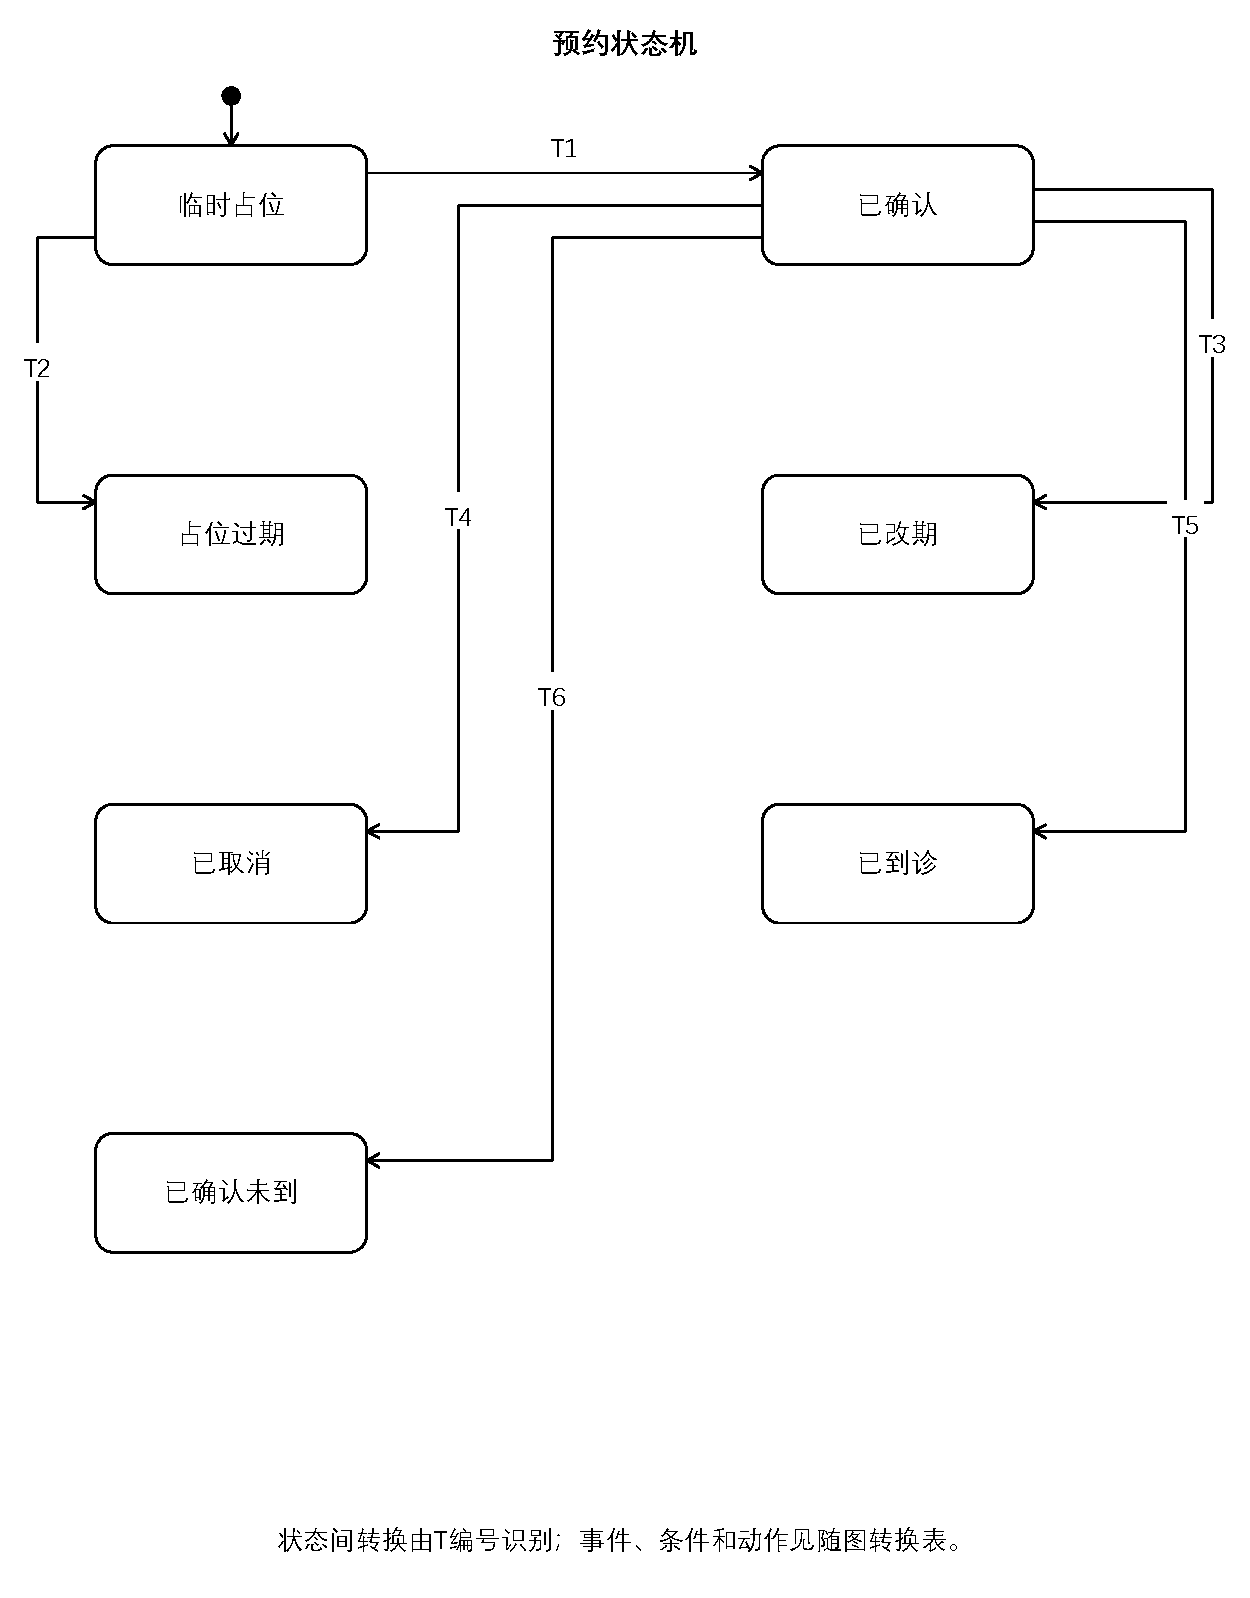
\includegraphics[width=\textwidth]{figures/st_appointment.pdf}
\caption{预约状态机}\label{st_appointment}\end{figure}
\par\noindent\begin{minipage}{\textwidth}
{\fontsize{10.5pt}{13.2pt}\selectfont\setlength{\tabcolsep}{0pt}\renewcommand{\arraystretch}{1.08}
\captionof{table}{预约状态机转换约定}\label{tab205}
\begin{tabular}{@{}p{1.140cm}@{\hspace{0.16cm}}p{4.840cm}@{\hspace{0.16cm}}p{9.140cm}@{}}
\toprule
\bfseries \Cell{编号} & \bfseries \Cell{源状态→目标状态} & \bfseries \Cell{事件、条件与动作}\\\midrule
\Cell{1} & \Cell{临时占位→已确认} & \Cell{完成核对且资源仍可用 /\allowbreak{} 建立正式预约}\\[1pt]
\Cell{2} & \Cell{临时占位→占位过期} & \Cell{超过占位期限 /\allowbreak{} 释放临时资源}\\[1pt]
\Cell{3} & \Cell{已确认→已改期} & \Cell{新安排确认成功 /\allowbreak{} 同事务释放旧安排}\\[1pt]
\Cell{4} & \Cell{已确认→已取消} & \Cell{取消获受理 /\allowbreak{} 留原因并释放资源}\\[1pt]
\Cell{5} & \Cell{已确认→已到诊} & \Cell{前台核实实际到诊 /\allowbreak{} 写到诊时间及true}\\[1pt]
\Cell{6} & \Cell{已确认→已确认未到} & \Cell{超过服务区间且前台核实未到 /\allowbreak{} 写原因}\\[1pt]
\bottomrule\end{tabular}
}\end{minipage}\par\vspace{6pt}
\begin{figure}[H]\centering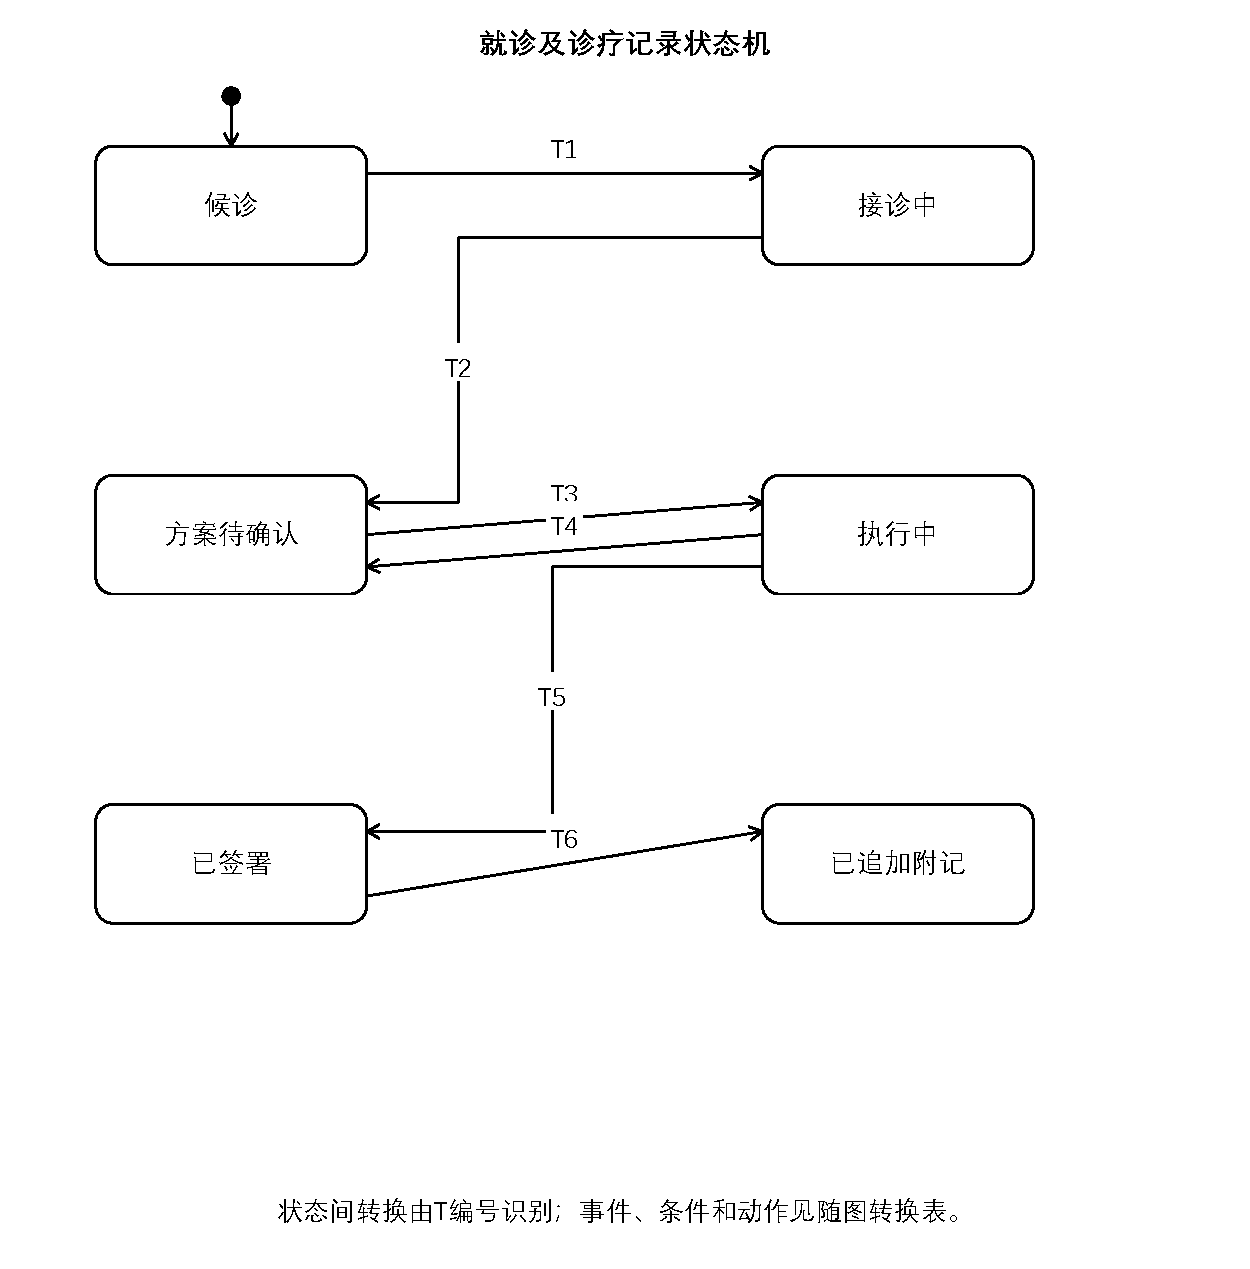
\includegraphics[width=\textwidth]{figures/st_visit.pdf}
\caption{就诊及诊疗记录状态机}\label{st_visit}\end{figure}
\par\noindent\begin{minipage}{\textwidth}
{\fontsize{10.5pt}{13.2pt}\selectfont\setlength{\tabcolsep}{0pt}\renewcommand{\arraystretch}{1.08}
\captionof{table}{就诊及诊疗记录状态机转换约定}\label{tab207}
\begin{tabular}{@{}p{1.140cm}@{\hspace{0.16cm}}p{4.840cm}@{\hspace{0.16cm}}p{9.140cm}@{}}
\toprule
\bfseries \Cell{编号} & \bfseries \Cell{源状态→目标状态} & \bfseries \Cell{事件、条件与动作}\\\midrule
\Cell{1} & \Cell{候诊→接诊中} & \Cell{医生接诊 /\allowbreak{} 核对患者与过敏}\\[1pt]
\Cell{2} & \Cell{接诊中→方案待确认} & \Cell{保存方案 /\allowbreak{} 固定待确认版本}\\[1pt]
\Cell{3} & \Cell{方案待确认→执行中} & \Cell{患者确认且阶段条件满足 /\allowbreak{} 开放执行}\\[1pt]
\Cell{4} & \Cell{执行中→方案待确认} & \Cell{提出增项 /\allowbreak{} 暂停新增项目等待确认}\\[1pt]
\Cell{5} & \Cell{执行中→已签署} & \Cell{医生完成核对 /\allowbreak{} 锁定记录并进入结算}\\[1pt]
\Cell{6} & \Cell{已签署→已追加附记} & \Cell{原签署人或获授权医生提出更正 /\allowbreak{} 追加附记}\\[1pt]
\bottomrule\end{tabular}
}\end{minipage}\par\vspace{6pt}
\begin{figure}[H]\centering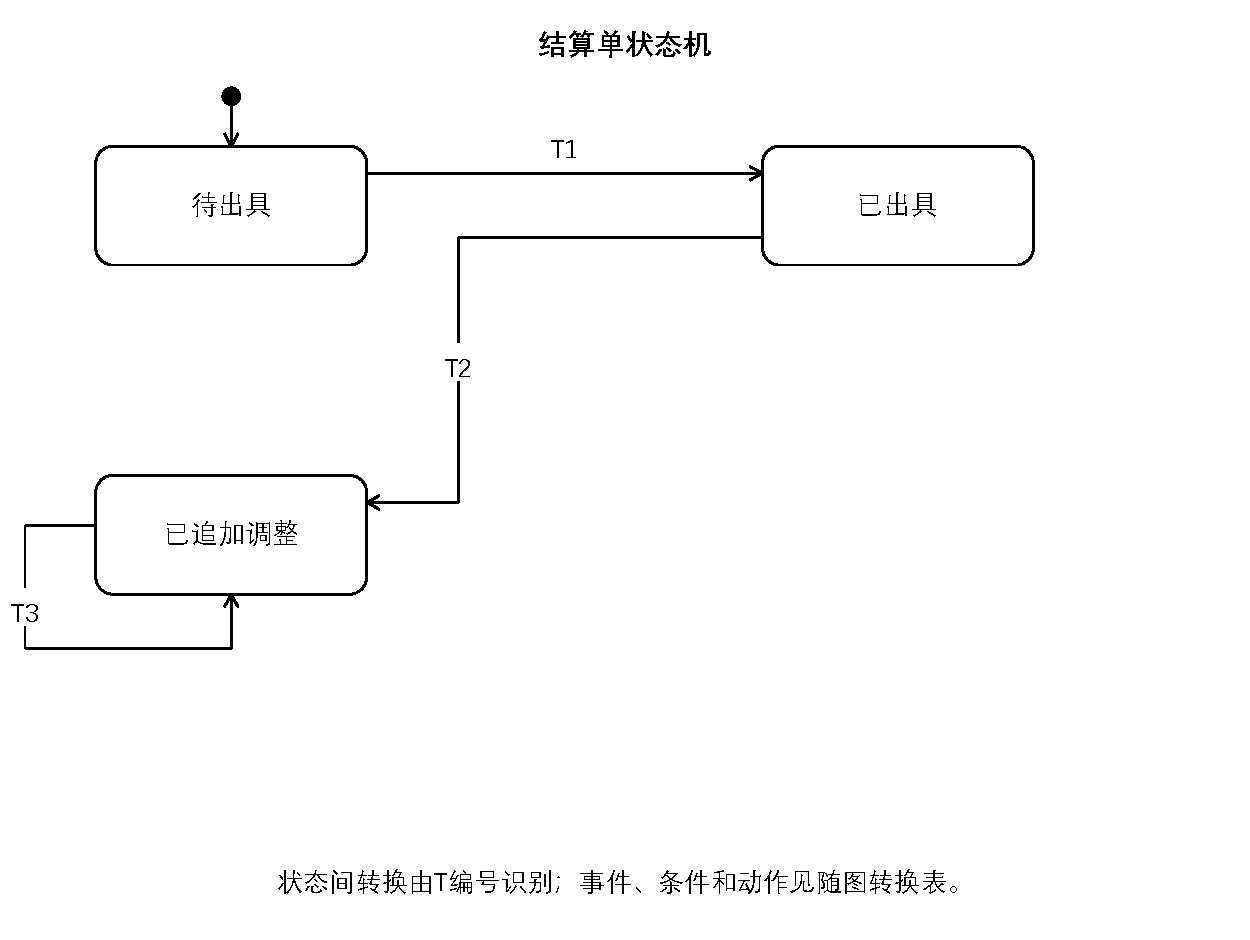
\includegraphics[width=\textwidth]{figures/st_invoice.pdf}
\caption{结算单状态机}\label{st_invoice}\end{figure}
\par\noindent\begin{minipage}{\textwidth}
{\fontsize{10.5pt}{13.2pt}\selectfont\setlength{\tabcolsep}{0pt}\renewcommand{\arraystretch}{1.08}
\captionof{table}{结算单状态机转换约定}\label{tab209}
\begin{tabular}{@{}p{1.140cm}@{\hspace{0.16cm}}p{4.840cm}@{\hspace{0.16cm}}p{9.140cm}@{}}
\toprule
\bfseries \Cell{编号} & \bfseries \Cell{源状态→目标状态} & \bfseries \Cell{事件、条件与动作}\\\midrule
\Cell{1} & \Cell{待出具→已出具} & \Cell{本次执行已签署 /\allowbreak{} 生成唯一单及逐行快照}\\[1pt]
\Cell{2} & \Cell{已出具→已追加调整} & \Cell{费用更正获独立批准 /\allowbreak{} 追加调整并更新净应收}\\[1pt]
\Cell{3} & \Cell{已追加调整→已追加调整} & \Cell{再次批准费用更正 /\allowbreak{} 以当前净额校验后追加；全额冲销仍保留原单}\\[1pt]
\bottomrule\end{tabular}
}\end{minipage}\par\vspace{6pt}
\begin{figure}[H]\centering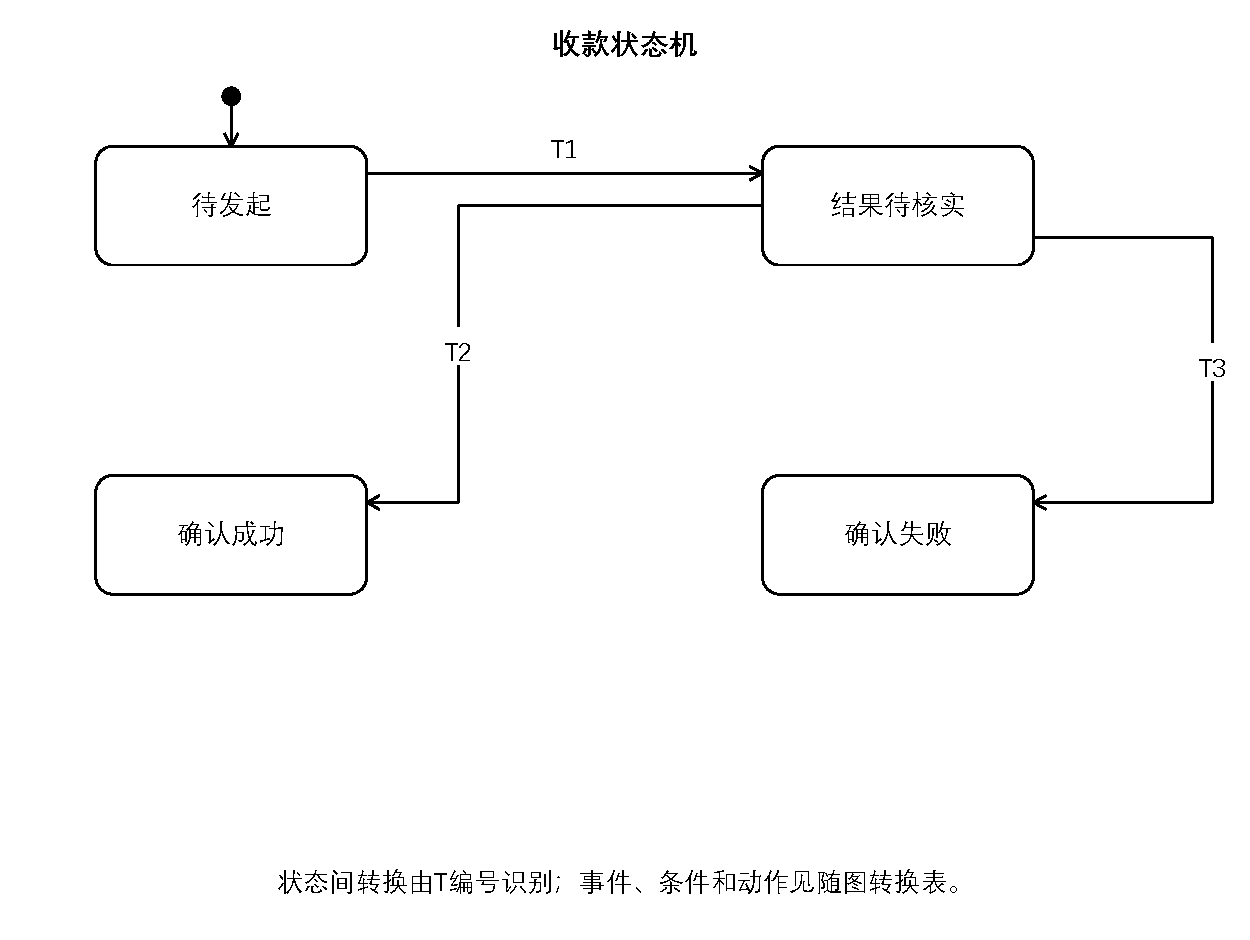
\includegraphics[width=\textwidth]{figures/st_payment.pdf}
\caption{收款状态机}\label{st_payment}\end{figure}
\par\noindent\begin{minipage}{\textwidth}
{\fontsize{10.5pt}{13.2pt}\selectfont\setlength{\tabcolsep}{0pt}\renewcommand{\arraystretch}{1.08}
\captionof{table}{收款状态机转换约定}\label{tab211}
\begin{tabular}{@{}p{1.140cm}@{\hspace{0.16cm}}p{4.840cm}@{\hspace{0.16cm}}p{9.140cm}@{}}
\toprule
\bfseries \Cell{编号} & \bfseries \Cell{源状态→目标状态} & \bfseries \Cell{事件、条件与动作}\\\midrule
\Cell{1} & \Cell{待发起→结果待核实} & \Cell{发起收款 /\allowbreak{} 保存唯一渠道请求}\\[1pt]
\Cell{2} & \Cell{结果待核实→确认成功} & \Cell{回调或查证确认成功 /\allowbreak{} 记录资金事实}\\[1pt]
\Cell{3} & \Cell{结果待核实→确认失败} & \Cell{查证确认失败 /\allowbreak{} 不形成实收}\\[1pt]
\bottomrule\end{tabular}
}\end{minipage}\par\vspace{6pt}
\begin{figure}[H]\centering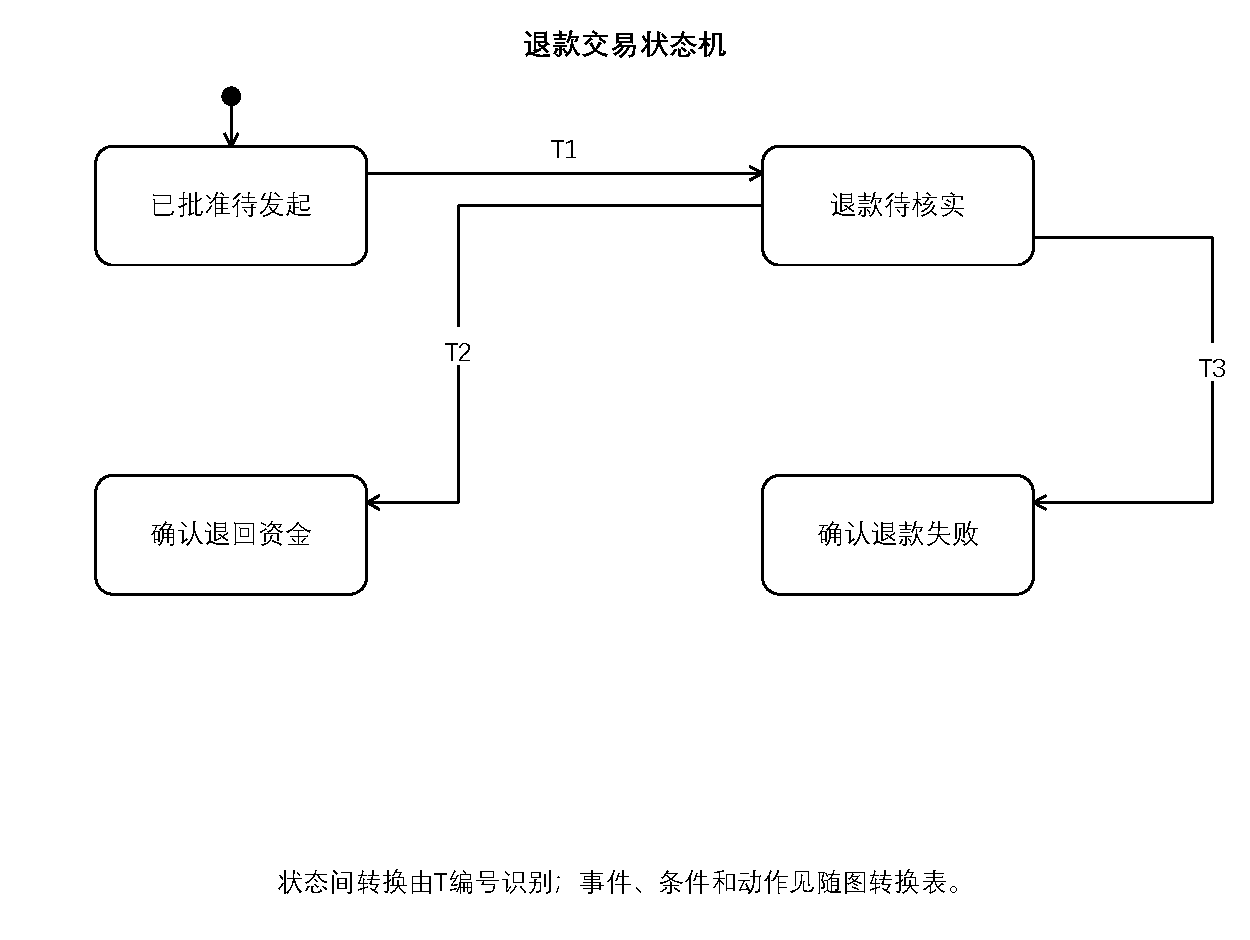
\includegraphics[width=\textwidth]{figures/st_refund.pdf}
\caption{退款交易状态机}\label{st_refund}\end{figure}
\par\noindent\begin{minipage}{\textwidth}
{\fontsize{10.5pt}{13.2pt}\selectfont\setlength{\tabcolsep}{0pt}\renewcommand{\arraystretch}{1.08}
\captionof{table}{退款交易状态机转换约定}\label{tab213}
\begin{tabular}{@{}p{1.140cm}@{\hspace{0.16cm}}p{4.840cm}@{\hspace{0.16cm}}p{9.140cm}@{}}
\toprule
\bfseries \Cell{编号} & \bfseries \Cell{源状态→目标状态} & \bfseries \Cell{事件、条件与动作}\\\midrule
\Cell{1} & \Cell{已批准待发起→退款待核实} & \Cell{审批有效且可退额已冻结 /\allowbreak{} 按原交易发起唯一退款请求}\\[1pt]
\Cell{2} & \Cell{退款待核实→确认退回资金} & \Cell{核验实际退款成功 /\allowbreak{} 追加资金结果}\\[1pt]
\Cell{3} & \Cell{退款待核实→确认退款失败} & \Cell{查证退款失败 /\allowbreak{} 释放冻结并保留重办依据}\\[1pt]
\bottomrule\end{tabular}
}\end{minipage}\par\vspace{6pt}
\begin{figure}[H]\centering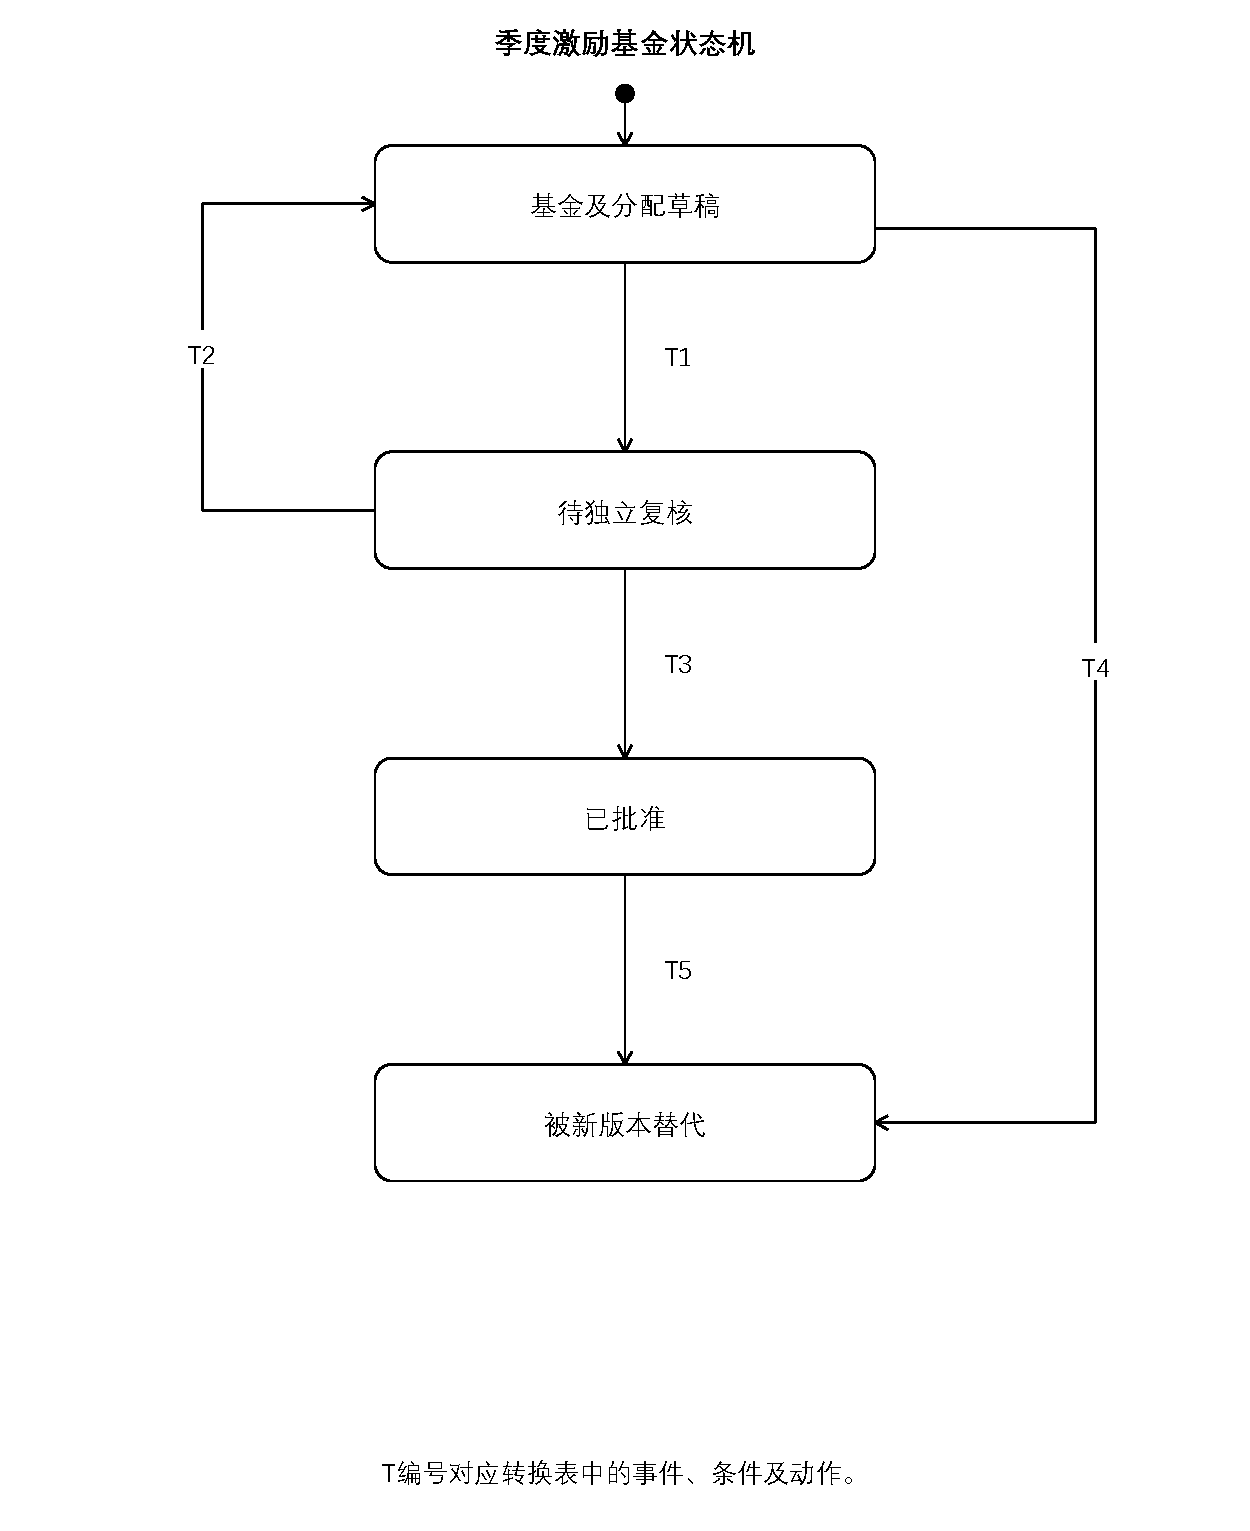
\includegraphics[width=\textwidth]{figures/st_quarter.pdf}
\caption{季度激励基金状态机}\label{st_quarter}\end{figure}
\par\noindent\begin{minipage}{\textwidth}
{\fontsize{10.5pt}{13.2pt}\selectfont\setlength{\tabcolsep}{0pt}\renewcommand{\arraystretch}{1.08}
\captionof{table}{季度激励基金状态机转换约定}\label{tab215}
\begin{tabular}{@{}p{1.140cm}@{\hspace{0.16cm}}p{4.840cm}@{\hspace{0.16cm}}p{9.140cm}@{}}
\toprule
\bfseries \Cell{编号} & \bfseries \Cell{源状态→目标状态} & \bfseries \Cell{事件、条件与动作}\\\midrule
\Cell{1} & \Cell{基金及分配草稿→待独立复核} & \Cell{经营月份关闭且来源和分配完整 /\allowbreak{} 固定送审版本}\\[1pt]
\Cell{2} & \Cell{待独立复核→基金及分配草稿} & \Cell{独立复核退回 /\allowbreak{} 保留原因并修订草稿}\\[1pt]
\Cell{3} & \Cell{待独立复核→已批准} & \Cell{独立批准 /\allowbreak{} 固定基金和个人额度，未等同实际发放}\\[1pt]
\Cell{4} & \Cell{基金及分配草稿→被新版本替代} & \Cell{来源变化 /\allowbreak{} 新建版本并保留原草稿}\\[1pt]
\Cell{5} & \Cell{已批准→被新版本替代} & \Cell{获准重开来源期间 /\allowbreak{} 新版重新复核，已有发放记录保留}\\[1pt]
\bottomrule\end{tabular}
}\end{minipage}\par\vspace{6pt}
\subsection{内部协作与操作契约}
每个用例采用边界—控制—实体的内部分析序列。边界处理交互及输入格式，控制类组织权限、仓储和事务，实体维护自身状态与业务不变量。分析序列中的实体操作由仓储加载后的领域对象承担；数据库查询及提交由应用服务调用数据映射器完成，不能把数据库当作替代业务判断的执行者。\par
类图展示关键属性与操作，连线标明业务关系和多重性，实心菱形表示组合；完整字段见用例规约及字典。内部序列用实线实心箭头表示调用、虚线开放箭头表示返回，alt分支需互斥，opt分支只在条件满足时发生。\par
\Needspace{497pt}
\subsubsection{UC-01 建立患者档案并核对逐项过敏}
边界：患者建档界面；控制：患者档案控制。\par
\begin{figure}[H]\centering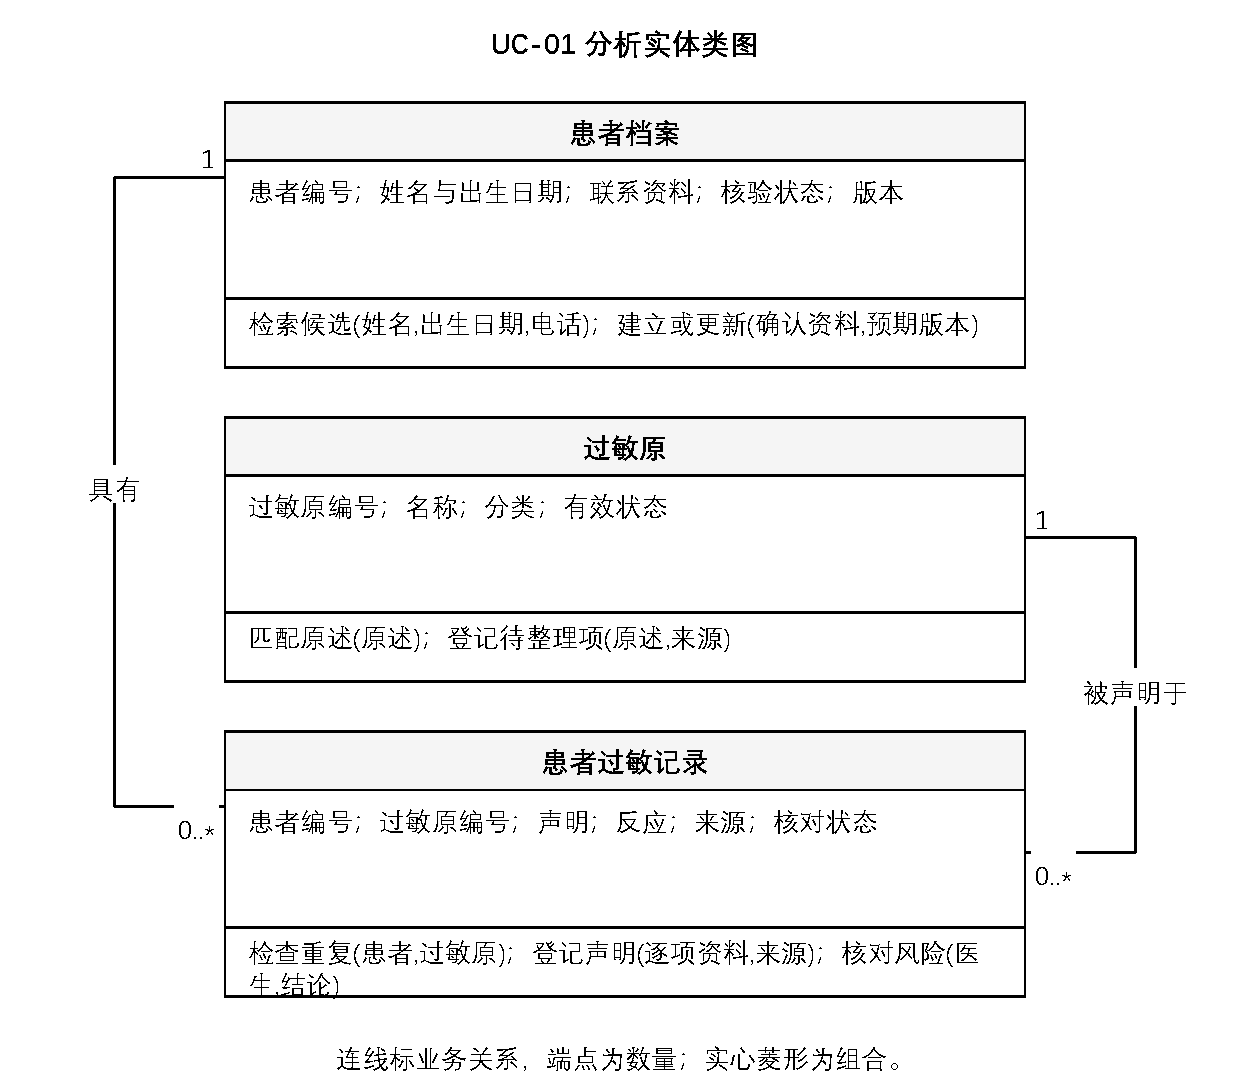
\includegraphics[width=\textwidth]{figures/class_UC_01.pdf}
\caption{UC-01 分析实体类图}\label{class_UC_01}\end{figure}
\begin{figure}[H]\centering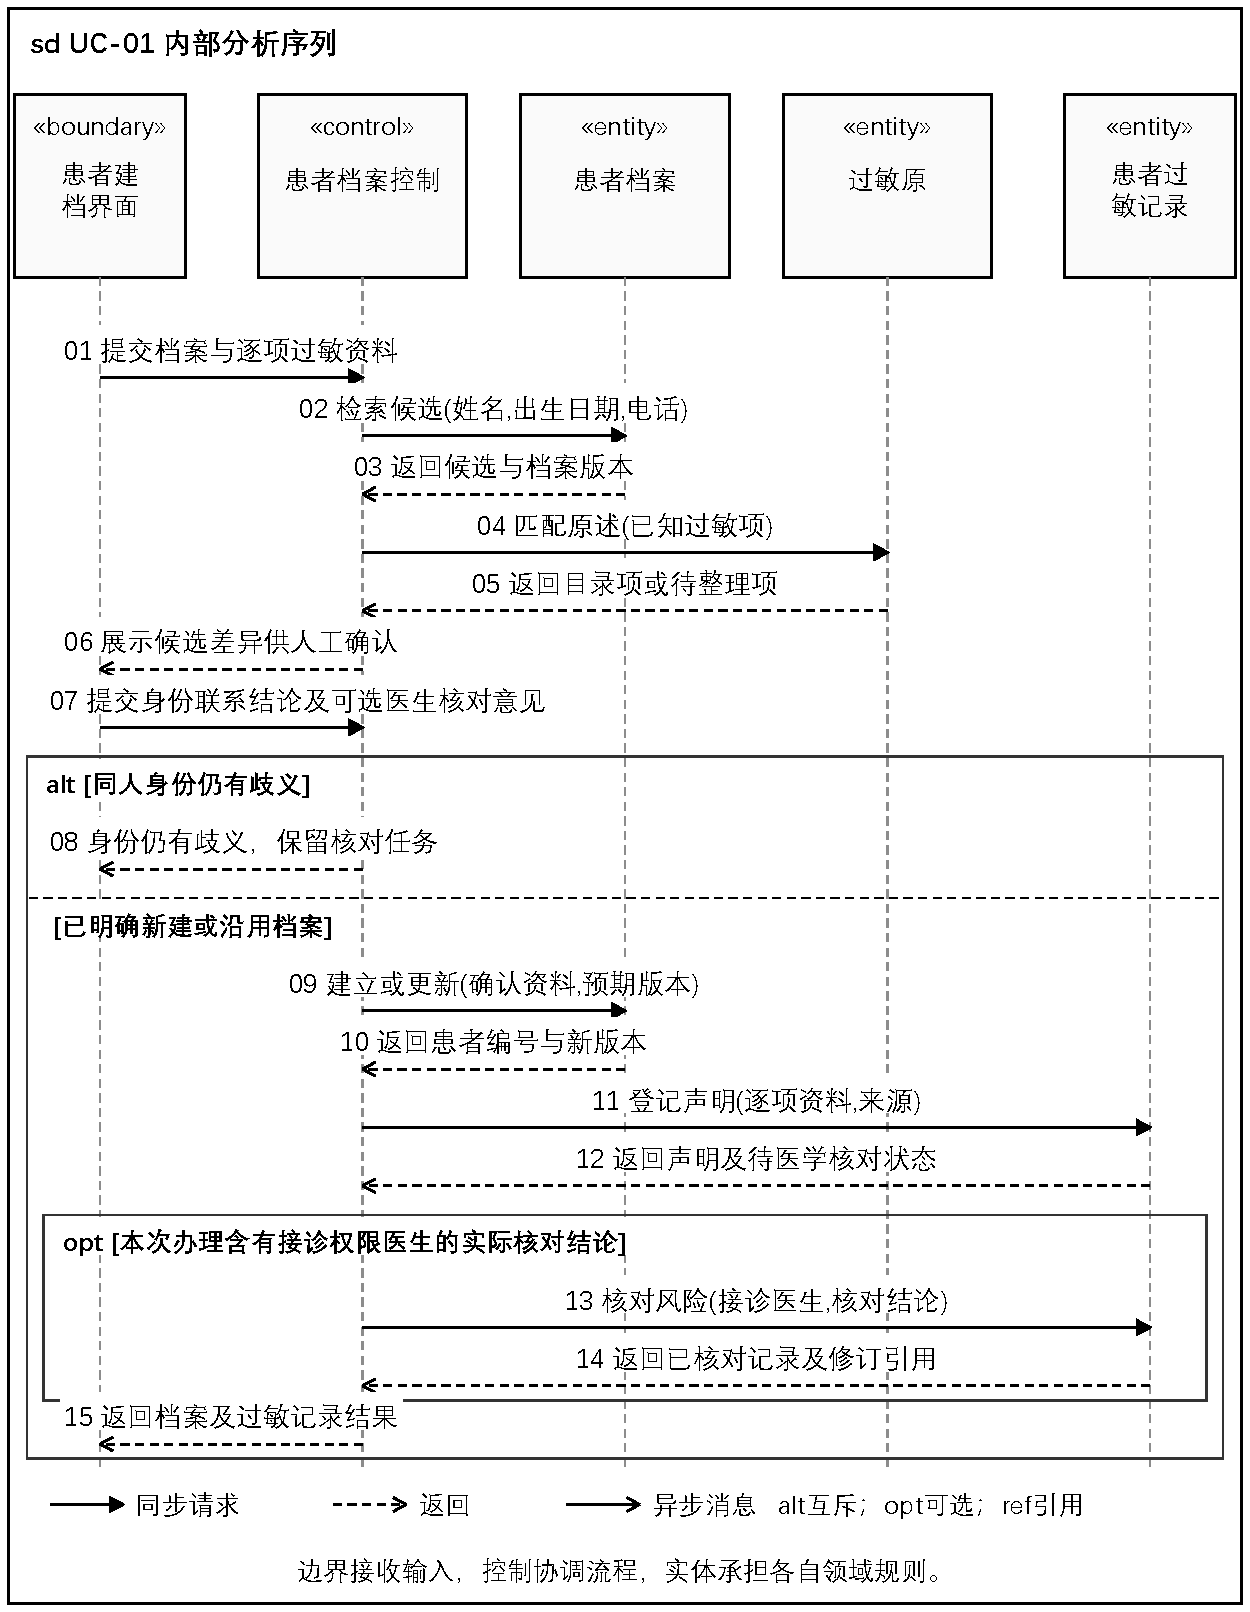
\includegraphics[width=\textwidth]{figures/seq_UC_01.pdf}
\caption{UC-01 内部分析序列}\label{seq_UC_01}\end{figure}
\par\noindent\begin{minipage}{\textwidth}
{\fontsize{10.5pt}{13.2pt}\selectfont\setlength{\tabcolsep}{0pt}\renewcommand{\arraystretch}{1.08}
\captionof{table}{UC-01操作契约 1}\label{tab223}
\begin{tabular}{@{}p{2.640cm}@{\hspace{0.16cm}}p{12.640cm}@{}}
\toprule
\bfseries \Cell{项目} & \bfseries \Cell{详细设计}\\\midrule
\Cell{签名} & \Cell{register\allowbreak{}Patient(\allowbreak{}command,\allowbreak{} actor,\allowbreak{} expected\allowbreak{}Version)\allowbreak{}}\\[1pt]
\Cell{输入} & \Cell{必要身份联系资料、逐项过敏、候选选择及声明来源}\\[1pt]
\Cell{执行前检查} & \Cell{本人或有效代办；员工按任务权限；存在候选时有核对结论}\\[1pt]
\Cell{成功结果} & \Cell{同一患者档案与本次过敏声明一起提交；不留下半份建档}\\[1pt]
\Cell{领域算法} & \Cell{先匹配候选及过敏目录，再区分新建、更新和待核对；锁定目标档案后查重并登记每项过敏；医生复核使用单独命令}\\[1pt]
\Cell{数据访问} & \Cell{Patient\allowbreak{}Repository装载患者与过敏聚合；patients、allergens、patient\_\allowbreak{}allergies分表，保存来源及修订链}\\[1pt]
\Cell{事务与并发} & \Cell{一短事务写患者及本次过敏条目；行版本冲突回滚；目录补充保留原述}\\[1pt]
\Cell{失败及恢复} & \Cell{IDENTITY\_\allowbreak{}PENDING保留核对任务；VERSION\_\allowbreak{}CONFLICT重新加载；无权限不返回候选明细}\\[1pt]
\bottomrule\end{tabular}
}\end{minipage}\par\vspace{6pt}
\par\noindent\begin{minipage}{\textwidth}
{\fontsize{10.5pt}{13.2pt}\selectfont\setlength{\tabcolsep}{0pt}\renewcommand{\arraystretch}{1.08}
\captionof{table}{UC-01操作契约 2}\label{tab224}
\begin{tabular}{@{}p{2.640cm}@{\hspace{0.16cm}}p{12.640cm}@{}}
\toprule
\bfseries \Cell{项目} & \bfseries \Cell{详细设计}\\\midrule
\Cell{签名} & \Cell{review\allowbreak{}Patient\allowbreak{}Allergies(\allowbreak{}patient\allowbreak{}Id,\allowbreak{} items,\allowbreak{} conclusion,\allowbreak{} expected\allowbreak{}Version)\allowbreak{}}\\[1pt]
\Cell{输入} & \Cell{逐项过敏及反应、医生核对结论与修订原因}\\[1pt]
\Cell{执行前检查} & \Cell{操作人为有当前接诊责任的合格医生}\\[1pt]
\Cell{成功结果} & \Cell{新增核对事实并保留原患者声明及修订链}\\[1pt]
\Cell{领域算法} & \Cell{逐项核对原述和反应；区别未知、否认与已知；产生修订而不覆盖旧记录}\\[1pt]
\Cell{数据访问} & \Cell{Patient\allowbreak{}Allergy\allowbreak{}Repository保存医生、时间和前版引用}\\[1pt]
\Cell{事务与并发} & \Cell{锁定患者过敏版本后同事务追加核对与当前有效引用}\\[1pt]
\Cell{失败及恢复} & \Cell{无接诊权限拒绝；版本变化重新核对，不自动采用旧结论}\\[1pt]
\bottomrule\end{tabular}
}\end{minipage}\par\vspace{6pt}
\par\noindent\begin{minipage}{\textwidth}
{\fontsize{10.5pt}{13.2pt}\selectfont\setlength{\tabcolsep}{0pt}\renewcommand{\arraystretch}{1.08}
\captionof{table}{UC-01表示与验收}\label{tab225}
\begin{tabular}{@{}p{2.640cm}@{\hspace{0.16cm}}p{12.640cm}@{}}
\toprule
\bfseries \Cell{项目} & \bfseries \Cell{设计}\\\midrule
\Cell{界面} & \Cell{以实际患者为页首；联系资料与逐项过敏分区，未知选项明确显示；复核动作只对接诊医生开放。}\\[1pt]
\Cell{接口} & \Cell{POST /\allowbreak{}auth/\allowbreak{}register 建立患者账号与资料；GET、PUT /\allowbreak{}patients/\allowbreak{}me 读取和更新本人资料，更新携带 expected\allowbreak{}Version；前台通过 GET、POST /\allowbreak{}staff/\allowbreak{}patients 核对或建档。}\\[1pt]
\Cell{验收场景} & \Cell{1.\allowbreak{} 家庭成员共用电话→生成不同患者编号。\\2.\allowbreak{} 同时更新同一档案→一个成功，另一得到版本冲突。\\3.\allowbreak{} 未知过敏→显示待核实，不生成无过敏结论。}\\[1pt]
\bottomrule\end{tabular}
}\end{minipage}\par\vspace{6pt}
\Needspace{497pt}
\subsubsection{UC-02 维护牙医档案与专业资格}
边界：牙医资格管理界面；控制：牙医资格控制。\par
\begin{figure}[H]\centering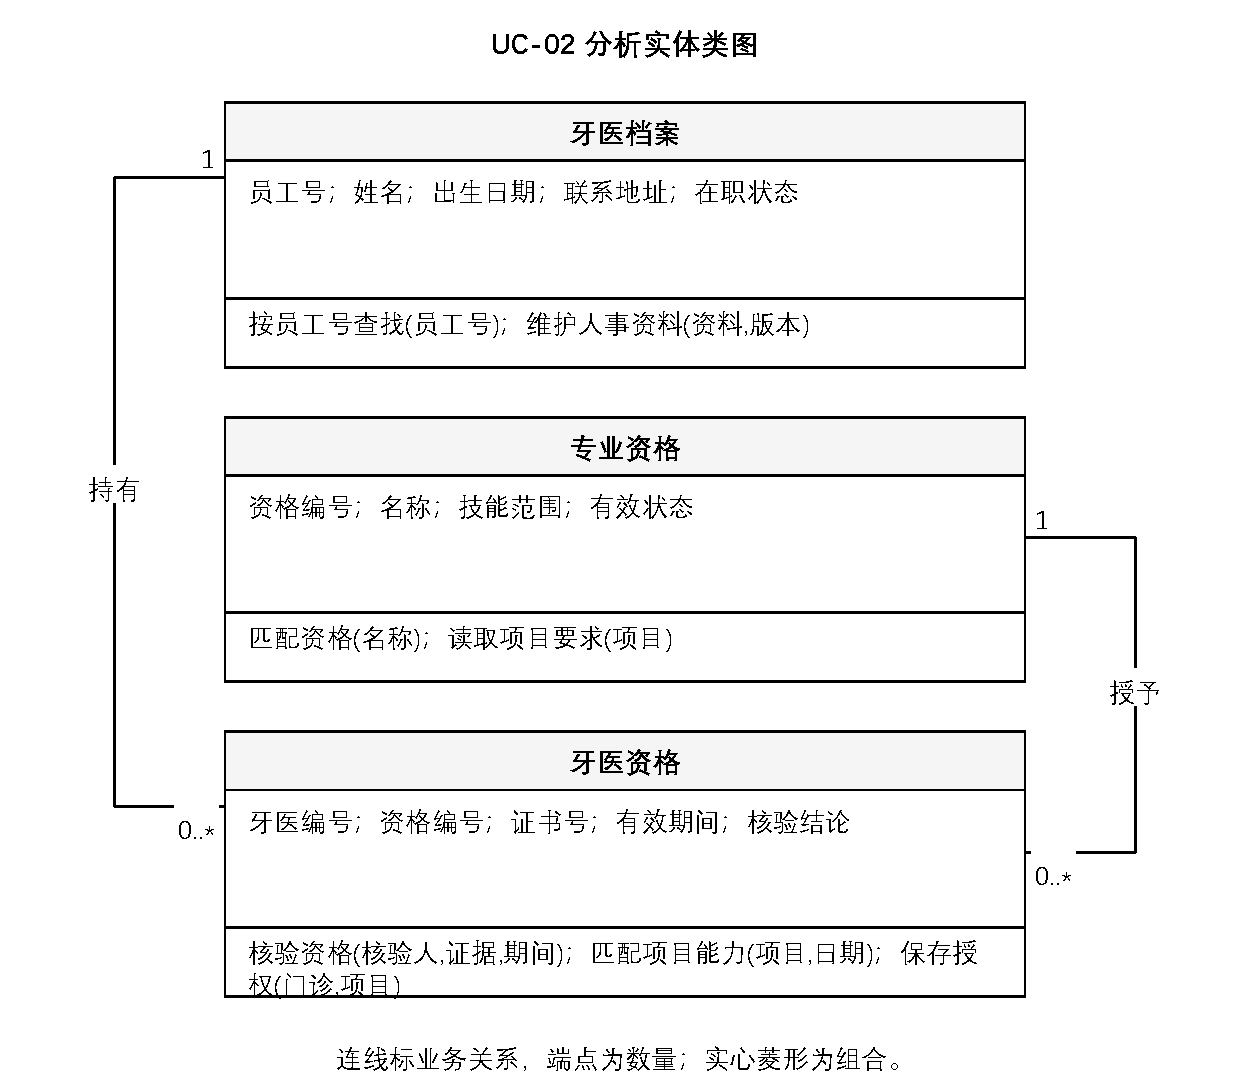
\includegraphics[width=\textwidth]{figures/class_UC_02.pdf}
\caption{UC-02 分析实体类图}\label{class_UC_02}\end{figure}
\begin{figure}[H]\centering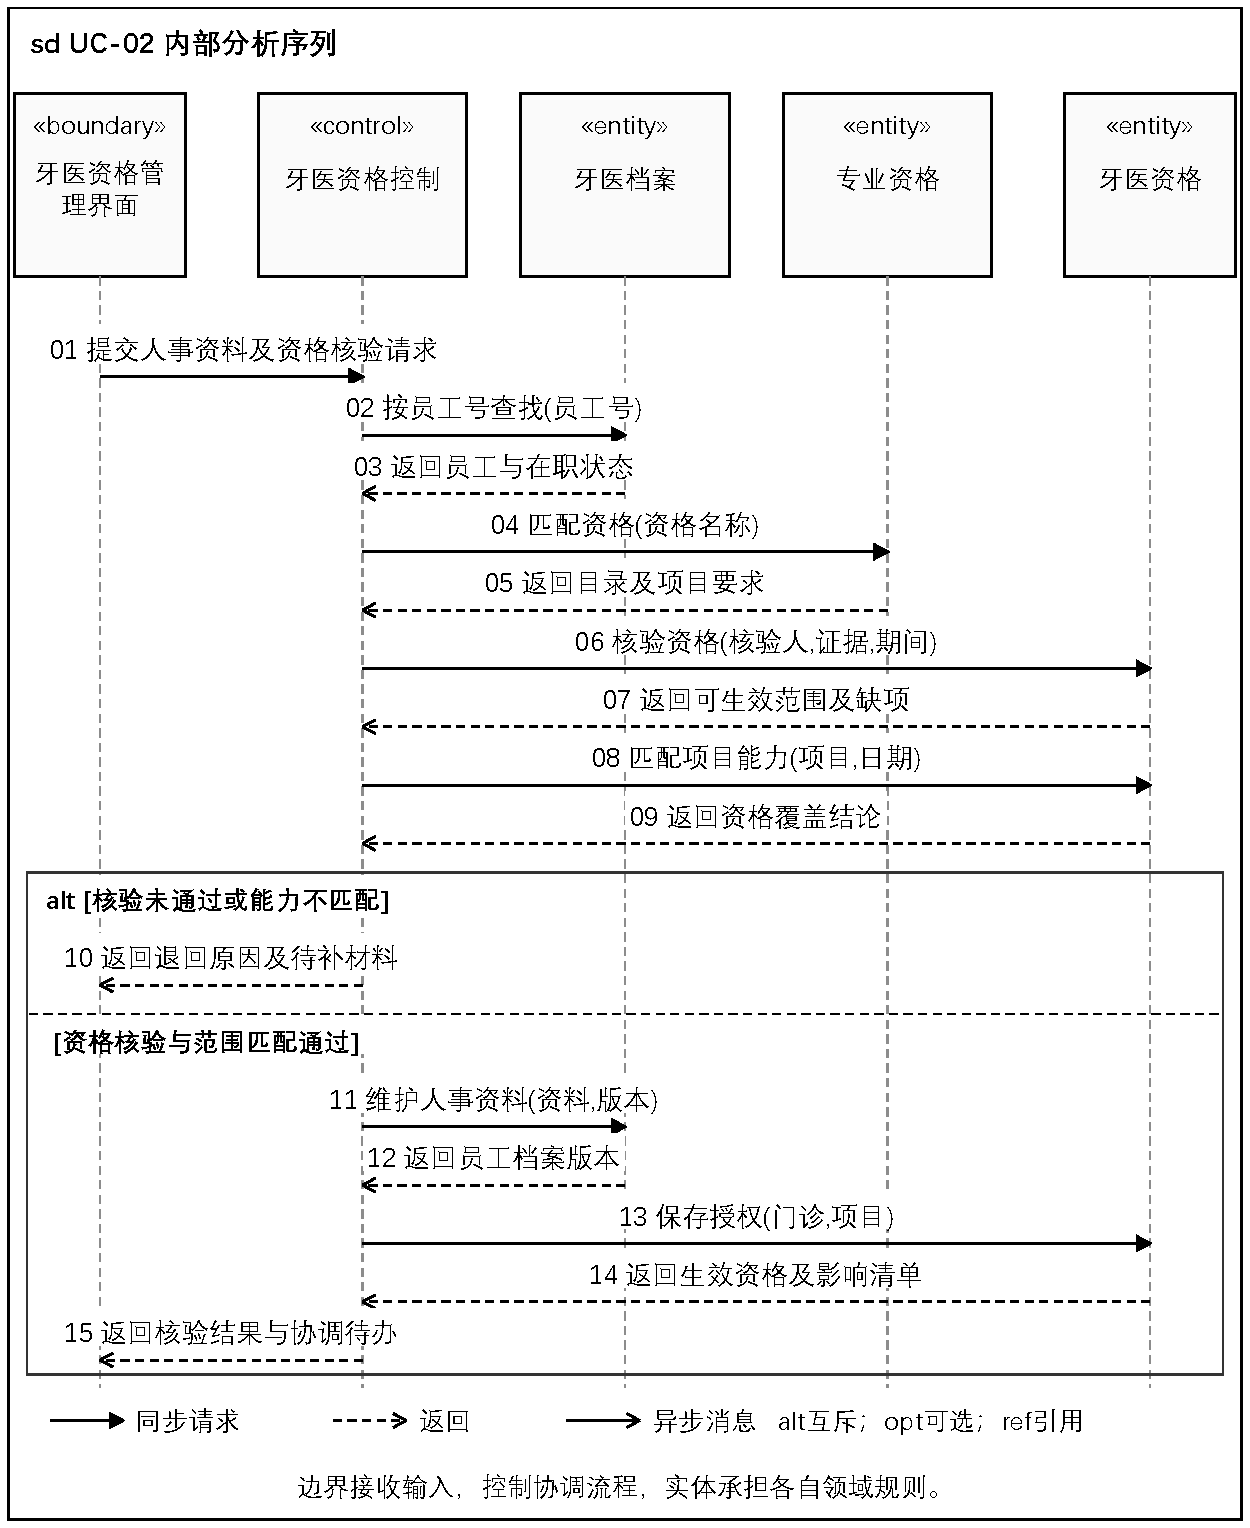
\includegraphics[width=\textwidth]{figures/seq_UC_02.pdf}
\caption{UC-02 内部分析序列}\label{seq_UC_02}\end{figure}
\par\noindent\begin{minipage}{\textwidth}
{\fontsize{10.5pt}{13.2pt}\selectfont\setlength{\tabcolsep}{0pt}\renewcommand{\arraystretch}{1.08}
\captionof{table}{UC-02操作契约}\label{tab230}
\begin{tabular}{@{}p{2.640cm}@{\hspace{0.16cm}}p{12.640cm}@{}}
\toprule
\bfseries \Cell{项目} & \bfseries \Cell{详细设计}\\\midrule
\Cell{签名} & \Cell{approve\allowbreak{}Dentist\allowbreak{}Qualification(\allowbreak{}dentist\allowbreak{}Id,\allowbreak{} credential,\allowbreak{} scope,\allowbreak{} actor)\allowbreak{}}\\[1pt]
\Cell{输入} & \Cell{证书材料、资格目录、适用项目和期间}\\[1pt]
\Cell{执行前检查} & \Cell{总部资格核验任务有效；被核验者有唯一员工档案}\\[1pt]
\Cell{成功结果} & \Cell{核验结论及范围生效，受影响预约进入协调清单}\\[1pt]
\Cell{领域算法} & \Cell{按证书和员工查重，检查有效期间及项目要求；通过才保存资格与项目授权；失效事件检索未来班次和预约}\\[1pt]
\Cell{数据访问} & \Cell{Dentist\allowbreak{}Repository与Qualification\allowbreak{}Repository；staff、qualifications、dentist\_\allowbreak{}qualifications，项目授权单独关联}\\[1pt]
\Cell{事务与并发} & \Cell{锁定牙医资格版本，核验及授权同事务提交；通知协调在提交后发送}\\[1pt]
\Cell{失败及恢复} & \Cell{CREDENTIAL\_\allowbreak{}DUPLICATE拒绝重复；EVIDENCE\_\allowbreak{}INCOMPLETE保留待补；SCOPE\_\allowbreak{}MISMATCH不发布能力}\\[1pt]
\bottomrule\end{tabular}
}\end{minipage}\par\vspace{6pt}
\par\noindent\begin{minipage}{\textwidth}
{\fontsize{10.5pt}{13.2pt}\selectfont\setlength{\tabcolsep}{0pt}\renewcommand{\arraystretch}{1.08}
\captionof{table}{UC-02表示与验收}\label{tab231}
\begin{tabular}{@{}p{2.640cm}@{\hspace{0.16cm}}p{12.640cm}@{}}
\toprule
\bfseries \Cell{项目} & \bfseries \Cell{设计}\\\midrule
\Cell{界面} & \Cell{人事资料与对外专长分区；资格列表显示证书、状态及截止日；变更前显示受影响预约数量。}\\[1pt]
\Cell{接口} & \Cell{GET /\allowbreak{}doctors、GET /\allowbreak{}qualifications 查询医生与资格；POST、PUT /\allowbreak{}staff/\allowbreak{}doctors 和 /\allowbreak{}staff/\allowbreak{}qualifications 维护授权范围内的医生与资格资料。}\\[1pt]
\Cell{验收场景} & \Cell{1.\allowbreak{} 一医生持多项资格→分别用于项目筛选。\\2.\allowbreak{} 同一证书重复提交→沿用待办，不重复授权。\\3.\allowbreak{} 证书到期且有未来预约→停止新增承诺并生成协调清单。}\\[1pt]
\bottomrule\end{tabular}
}\end{minipage}\par\vspace{6pt}
\Needspace{497pt}
\subsubsection{UC-03 维护治疗目录与标准单位价格}
边界：治疗目录管理界面；控制：治疗标准控制。\par
\begin{figure}[H]\centering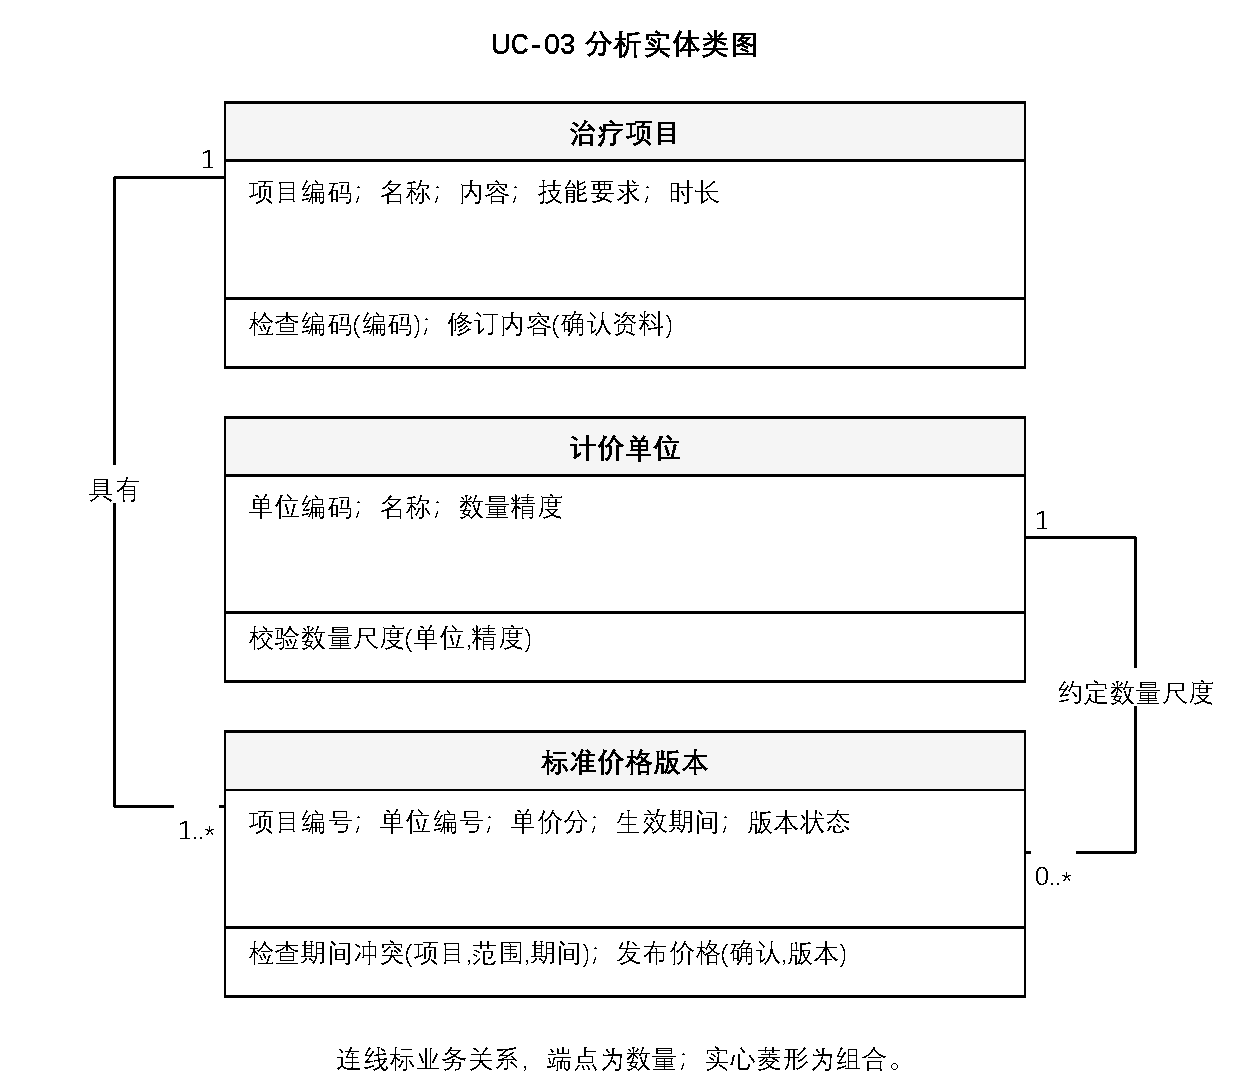
\includegraphics[width=\textwidth]{figures/class_UC_03.pdf}
\caption{UC-03 分析实体类图}\label{class_UC_03}\end{figure}
\begin{figure}[H]\centering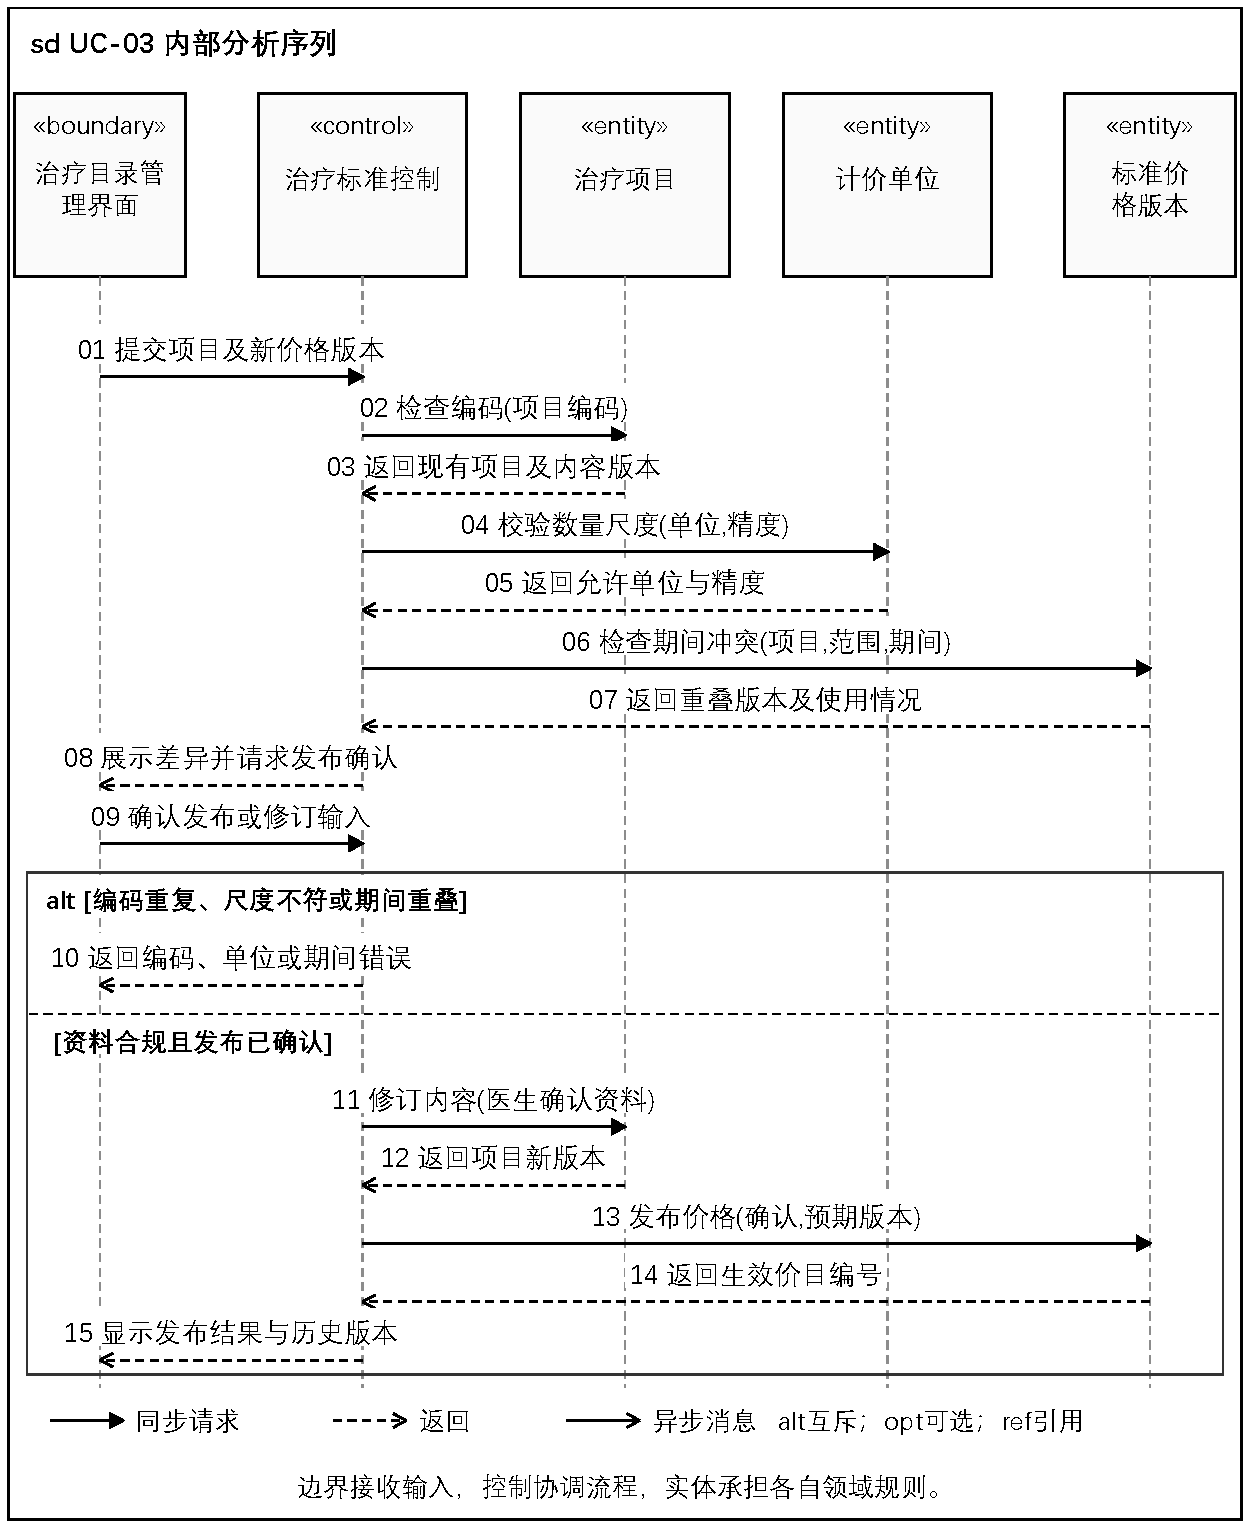
\includegraphics[width=\textwidth]{figures/seq_UC_03.pdf}
\caption{UC-03 内部分析序列}\label{seq_UC_03}\end{figure}
\par\noindent\begin{minipage}{\textwidth}
{\fontsize{10.5pt}{13.2pt}\selectfont\setlength{\tabcolsep}{0pt}\renewcommand{\arraystretch}{1.08}
\captionof{table}{UC-03操作契约}\label{tab236}
\begin{tabular}{@{}p{2.640cm}@{\hspace{0.16cm}}p{12.640cm}@{}}
\toprule
\bfseries \Cell{项目} & \bfseries \Cell{详细设计}\\\midrule
\Cell{签名} & \Cell{publish\allowbreak{}Treatment\allowbreak{}Price(\allowbreak{}item\allowbreak{}Id,\allowbreak{} unit,\allowbreak{} price\allowbreak{}Cents,\allowbreak{} period,\allowbreak{} expected\allowbreak{}Version)\allowbreak{}}\\[1pt]
\Cell{输入} & \Cell{项目内容、医生确认及标准单位、整数分价格、生效期间}\\[1pt]
\Cell{执行前检查} & \Cell{总部维护权限有效；单位与项目规定一致}\\[1pt]
\Cell{成功结果} & \Cell{新价目发布且历史引用不变，同范围期间无交叠}\\[1pt]
\Cell{领域算法} & \Cell{按项目与范围读取既有价目并比对期间；显示差异后按版本创建新价，旧价按边界截止}\\[1pt]
\Cell{数据访问} & \Cell{Treatment\allowbreak{}Catalog\allowbreak{}Repository与Price\allowbreak{}Repository；services保存standard\_\allowbreak{}unit与quantity\_\allowbreak{}scale，service\_\allowbreak{}prices保存生效价格版本；历史执行与账单保存单位及单价来源快照。}\\[1pt]
\Cell{事务与并发} & \Cell{发布在短事务内锁定项目定价范围；冲突检查与新增版本一次提交}\\[1pt]
\Cell{失败及恢复} & \Cell{DUPLICATE\_\allowbreak{}CODE返回原项；PERIOD\_\allowbreak{}OVERLAP拒绝发布；VERSION\_\allowbreak{}CONFLICT重新比较}\\[1pt]
\bottomrule\end{tabular}
}\end{minipage}\par\vspace{6pt}
\par\noindent\begin{minipage}{\textwidth}
{\fontsize{10.5pt}{13.2pt}\selectfont\setlength{\tabcolsep}{0pt}\renewcommand{\arraystretch}{1.08}
\captionof{table}{UC-03表示与验收}\label{tab237}
\begin{tabular}{@{}p{2.640cm}@{\hspace{0.16cm}}p{12.640cm}@{}}
\toprule
\bfseries \Cell{项目} & \bfseries \Cell{设计}\\\midrule
\Cell{界面} & \Cell{并排显示现行和拟发布的单位、单价与生效日期；历史页只读；临床内容确认与价目发布分别署名。}\\[1pt]
\Cell{接口} & \Cell{GET /\allowbreak{}services 查询服务；POST、PUT /\allowbreak{}staff/\allowbreak{}services 维护项目、时长与资格要求；GET /\allowbreak{}treatment-\allowbreak{}references 提供独立的治疗参考价。}\\[1pt]
\Cell{验收场景} & \Cell{1.\allowbreak{} 把单位从次改为牙→建立新版本，旧执行仍按次。\\2.\allowbreak{} 两个发布请求覆盖同一期间→仅一个通过。\\3.\allowbreak{} 价格100元调整为120元→原已确认快照仍为100元。}\\[1pt]
\bottomrule\end{tabular}
}\end{minipage}\par\vspace{6pt}
\Needspace{497pt}
\subsubsection{UC-04 编排跨店医生班次并发布容量}
边界：跨店排班界面；控制：出诊编排控制。\par
\begin{figure}[H]\centering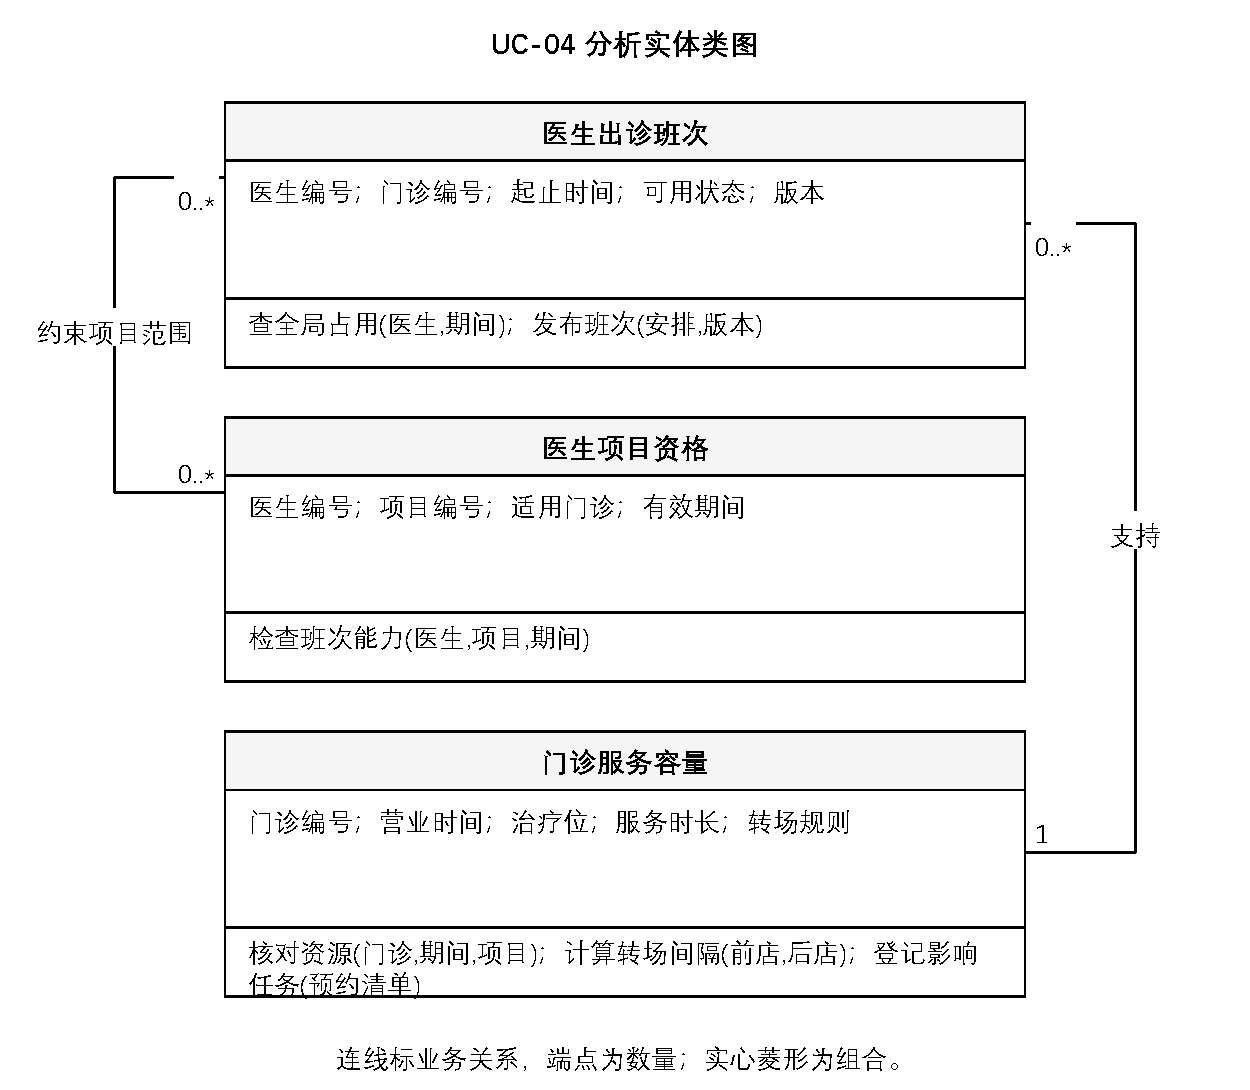
\includegraphics[width=\textwidth]{figures/class_UC_04.pdf}
\caption{UC-04 分析实体类图}\label{class_UC_04}\end{figure}
\begin{figure}[H]\centering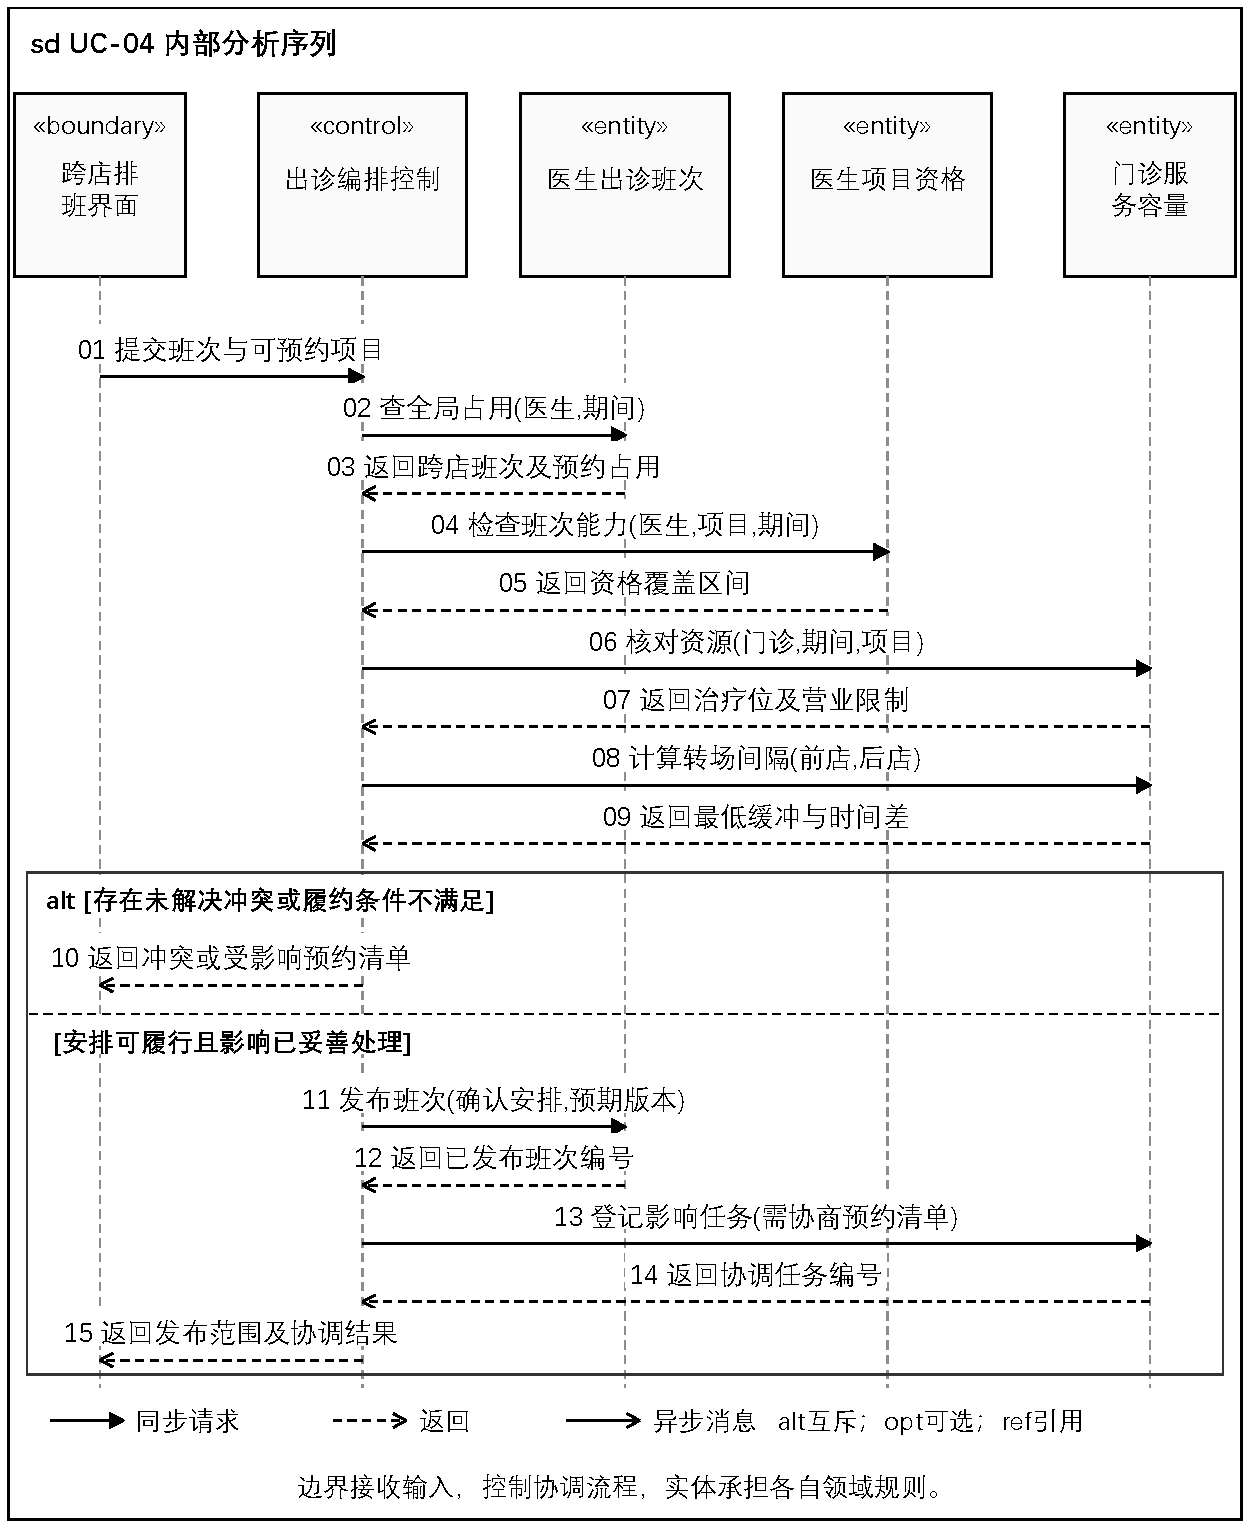
\includegraphics[width=\textwidth]{figures/seq_UC_04.pdf}
\caption{UC-04 内部分析序列}\label{seq_UC_04}\end{figure}
\par\noindent\begin{minipage}{\textwidth}
{\fontsize{10.5pt}{13.2pt}\selectfont\setlength{\tabcolsep}{0pt}\renewcommand{\arraystretch}{1.08}
\captionof{table}{UC-04操作契约}\label{tab242}
\begin{tabular}{@{}p{2.640cm}@{\hspace{0.16cm}}p{12.640cm}@{}}
\toprule
\bfseries \Cell{项目} & \bfseries \Cell{详细设计}\\\midrule
\Cell{签名} & \Cell{publish\allowbreak{}Dentist\allowbreak{}Shift(\allowbreak{}dentist\allowbreak{}Id,\allowbreak{} clinic\allowbreak{}Id,\allowbreak{} interval,\allowbreak{} services,\allowbreak{} expected\allowbreak{}Version)\allowbreak{}}\\[1pt]
\Cell{输入} & \Cell{医生、门诊、项目、时间及转场规则版本}\\[1pt]
\Cell{执行前检查} & \Cell{排班任务权限有效；涉及旧预约的调整有协调依据}\\[1pt]
\Cell{成功结果} & \Cell{无全局重叠班次，可预约容量与资格资源一致}\\[1pt]
\Cell{领域算法} & \Cell{按医生锁定全局排班范围，比较重叠及相邻异店间隔；按整段有效资格过滤项目，再计算本店治疗位容量并发布}\\[1pt]
\Cell{数据访问} & \Cell{Schedule\allowbreak{}Repository按医生及时间范围查询全连锁安排；doctor\_\allowbreak{}shifts、chairs及doctor\_\allowbreak{}shift\_\allowbreak{}services保存班次、资源与开放项目，受影响预约以任务和审计事件引用。}\\[1pt]
\Cell{事务与并发} & \Cell{同一医生的跨店排班以一致锁顺序提交；班次版本与容量一起生效，通知在事务后发送}\\[1pt]
\Cell{失败及恢复} & \Cell{SHIFT\_\allowbreak{}OVERLAP或TRAVEL\_\allowbreak{}GAP不发布；QUALIFICATION\_\allowbreak{}EXPIRED缩小项目；APPOINTMENT\_\allowbreak{}IMPACT要求协调}\\[1pt]
\bottomrule\end{tabular}
}\end{minipage}\par\vspace{6pt}
\par\noindent\begin{minipage}{\textwidth}
{\fontsize{10.5pt}{13.2pt}\selectfont\setlength{\tabcolsep}{0pt}\renewcommand{\arraystretch}{1.08}
\captionof{table}{UC-04表示与验收}\label{tab243}
\begin{tabular}{@{}p{2.640cm}@{\hspace{0.16cm}}p{12.640cm}@{}}
\toprule
\bfseries \Cell{项目} & \bfseries \Cell{设计}\\\midrule
\Cell{界面} & \Cell{全局时间轴显示医生跨店班次，门诊用文字标识；冲突行可定位资格、资源或转场原因。}\\[1pt]
\Cell{接口} & \Cell{GET /\allowbreak{}shifts 查询排班；POST /\allowbreak{}staff/\allowbreak{}shifts 发布班次，POST /\allowbreak{}staff/\allowbreak{}shifts/\allowbreak{}\{id\}/\allowbreak{}cancel 撤销班次。服务端校验门诊授权、资格、跨店时间及转场。}\\[1pt]
\Cell{验收场景} & \Cell{1.\allowbreak{} 同一医生异店班次重叠→拒绝第二次发布。\\2.\allowbreak{} 相邻异店班次不足转场缓冲→提示间隔缺口。\\3.\allowbreak{} 缩班影响预约→未完成协调时原预约保持。}\\[1pt]
\bottomrule\end{tabular}
}\end{minipage}\par\vspace{6pt}
\Needspace{497pt}
\subsubsection{UC-05 查询匹配的可预约时段}
边界：预约时段查询界面；控制：号源匹配控制。\par
\begin{figure}[H]\centering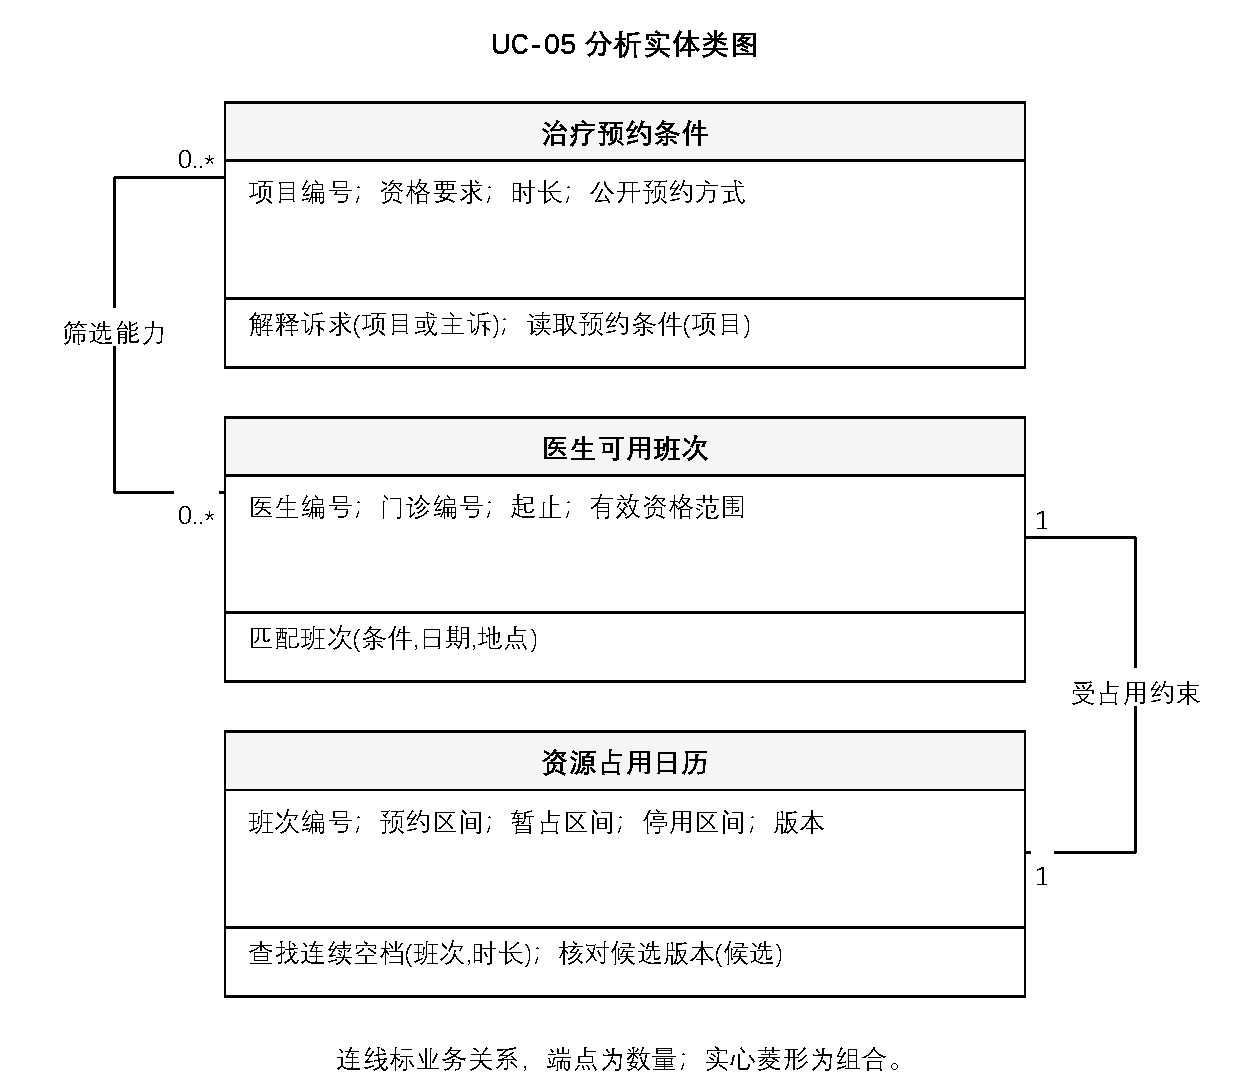
\includegraphics[width=\textwidth]{figures/class_UC_05.pdf}
\caption{UC-05 分析实体类图}\label{class_UC_05}\end{figure}
\begin{figure}[H]\centering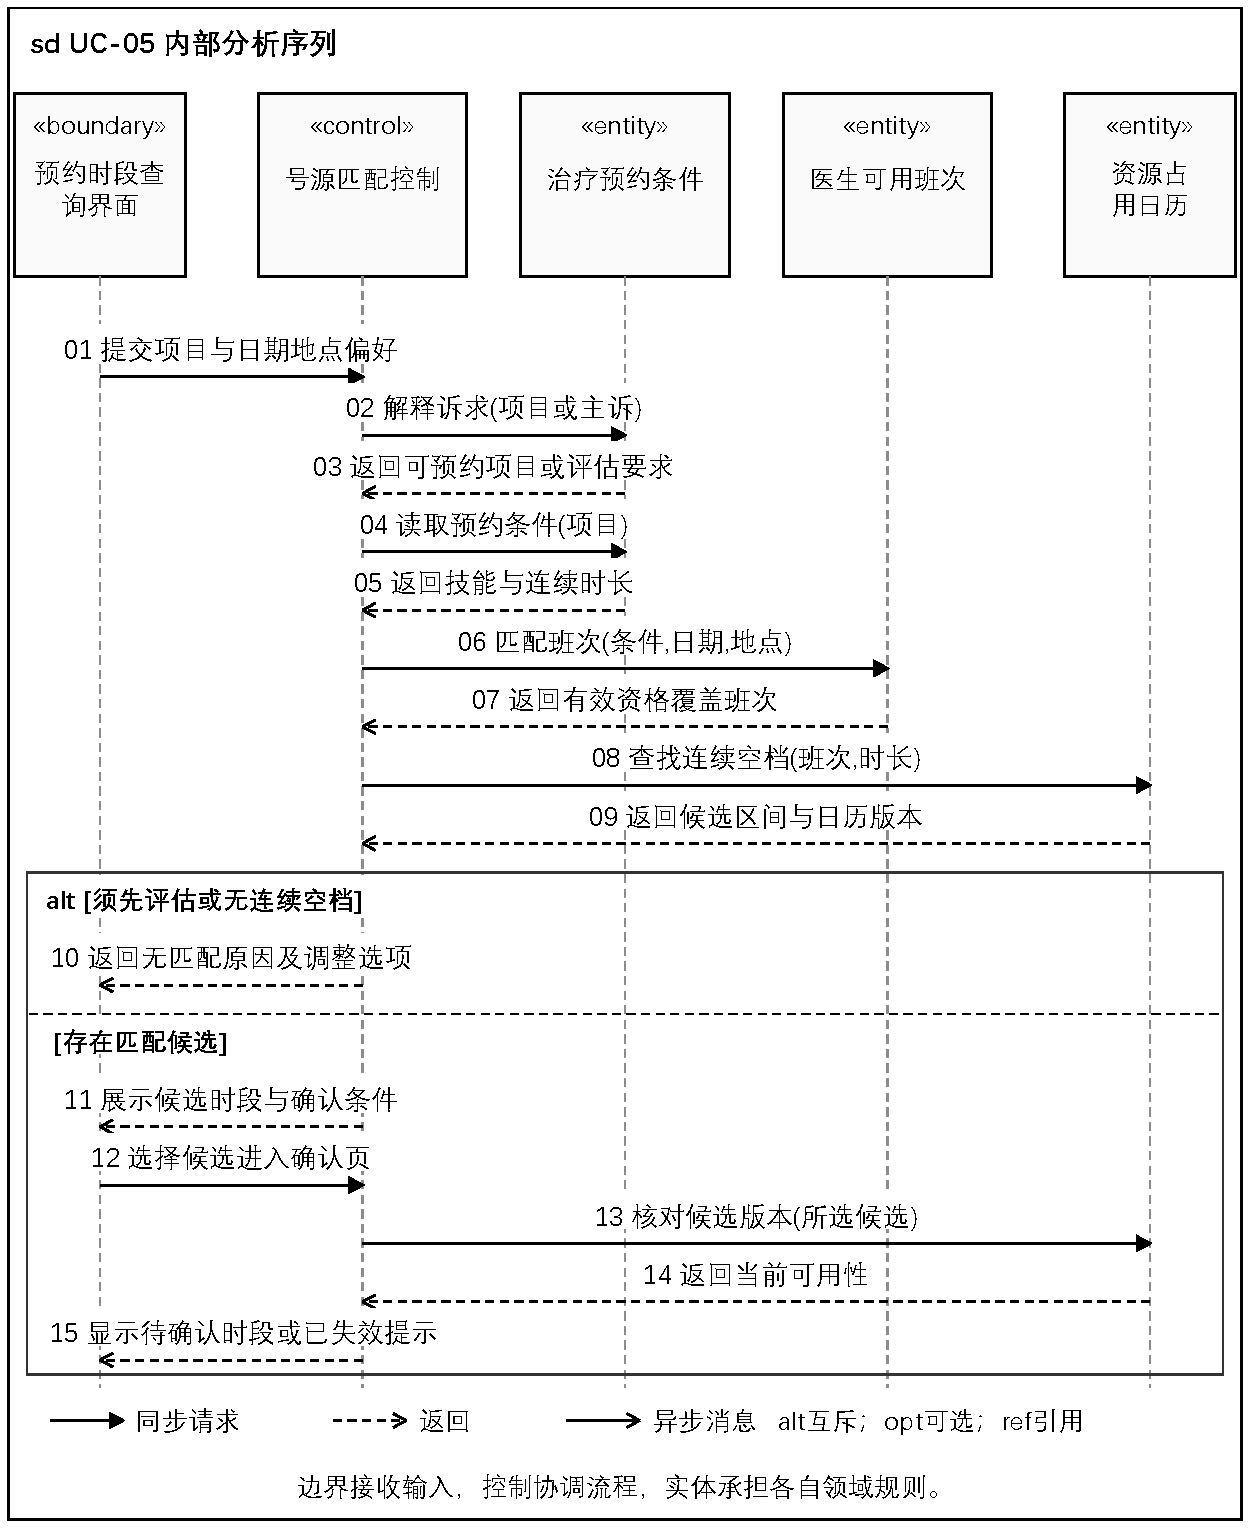
\includegraphics[width=\textwidth]{figures/seq_UC_05.pdf}
\caption{UC-05 内部分析序列}\label{seq_UC_05}\end{figure}
\par\noindent\begin{minipage}{\textwidth}
{\fontsize{10.5pt}{13.2pt}\selectfont\setlength{\tabcolsep}{0pt}\renewcommand{\arraystretch}{1.08}
\captionof{table}{UC-05操作契约}\label{tab248}
\begin{tabular}{@{}p{2.640cm}@{\hspace{0.16cm}}p{12.640cm}@{}}
\toprule
\bfseries \Cell{项目} & \bfseries \Cell{详细设计}\\\midrule
\Cell{签名} & \Cell{find\allowbreak{}Bookable\allowbreak{}Slots(\allowbreak{}criteria,\allowbreak{} actor)\allowbreak{}}\\[1pt]
\Cell{输入} & \Cell{项目或主诉、日期区间、门诊与医生偏好}\\[1pt]
\Cell{执行前检查} & \Cell{查询日期在允许窗口内；项目公开范围可查询}\\[1pt]
\Cell{成功结果} & \Cell{只返回符合资格、排班和资源约束的候选，无写入占用}\\[1pt]
\Cell{领域算法} & \Cell{先解析项目预约方式，按技能和门诊过滤班次，再按区间合并占用并求连续空档；返回候选时附版本及估价}\\[1pt]
\Cell{数据访问} & \Cell{Slot\allowbreak{}Query\allowbreak{}Service连接治疗、资格、班次和占用索引，直接投影候选DTO；不装载其他患者资料}\\[1pt]
\Cell{事务与并发} & \Cell{只读一致性快照；查询不加业务占用锁；确认预约另行重新校验}\\[1pt]
\Cell{失败及恢复} & \Cell{ASSESSMENT\_\allowbreak{}REQUIRED引导评估；NO\_\allowbreak{}SLOT提供调整条件；RANGE\_\allowbreak{}TOO\_\allowbreak{}LARGE要求缩小范围}\\[1pt]
\bottomrule\end{tabular}
}\end{minipage}\par\vspace{6pt}
\par\noindent\begin{minipage}{\textwidth}
{\fontsize{10.5pt}{13.2pt}\selectfont\setlength{\tabcolsep}{0pt}\renewcommand{\arraystretch}{1.08}
\captionof{table}{UC-05表示与验收}\label{tab249}
\begin{tabular}{@{}p{2.640cm}@{\hspace{0.16cm}}p{12.640cm}@{}}
\toprule
\bfseries \Cell{项目} & \bfseries \Cell{设计}\\\midrule
\Cell{界面} & \Cell{日期、门诊和医生筛选相互联动；空结果展示可调整条件；选择后进入确认页，查询页不显示预约成功。}\\[1pt]
\Cell{接口} & \Cell{GET /\allowbreak{}booking-\allowbreak{}policy 返回规则与日期查询范围；GET /\allowbreak{}booking-\allowbreak{}slots 按 clinic\allowbreak{}Id、service\allowbreak{}Id、date 及可选 doctor\allowbreak{}Id 查询候选时段。}\\[1pt]
\Cell{验收场景} & \Cell{1.\allowbreak{} 医生空闲但治疗位不可用→不返回该时段。\\2.\allowbreak{} 项目要求45分钟而仅空30分钟→不生成候选。\\3.\allowbreak{} 查询后被他人预约→确认页提示刷新，不出现重复承诺。}\\[1pt]
\bottomrule\end{tabular}
}\end{minipage}\par\vspace{6pt}
\Needspace{497pt}
\subsubsection{UC-06 确认患者预约}
边界：预约确认界面；控制：预约确认控制。\par
\begin{figure}[H]\centering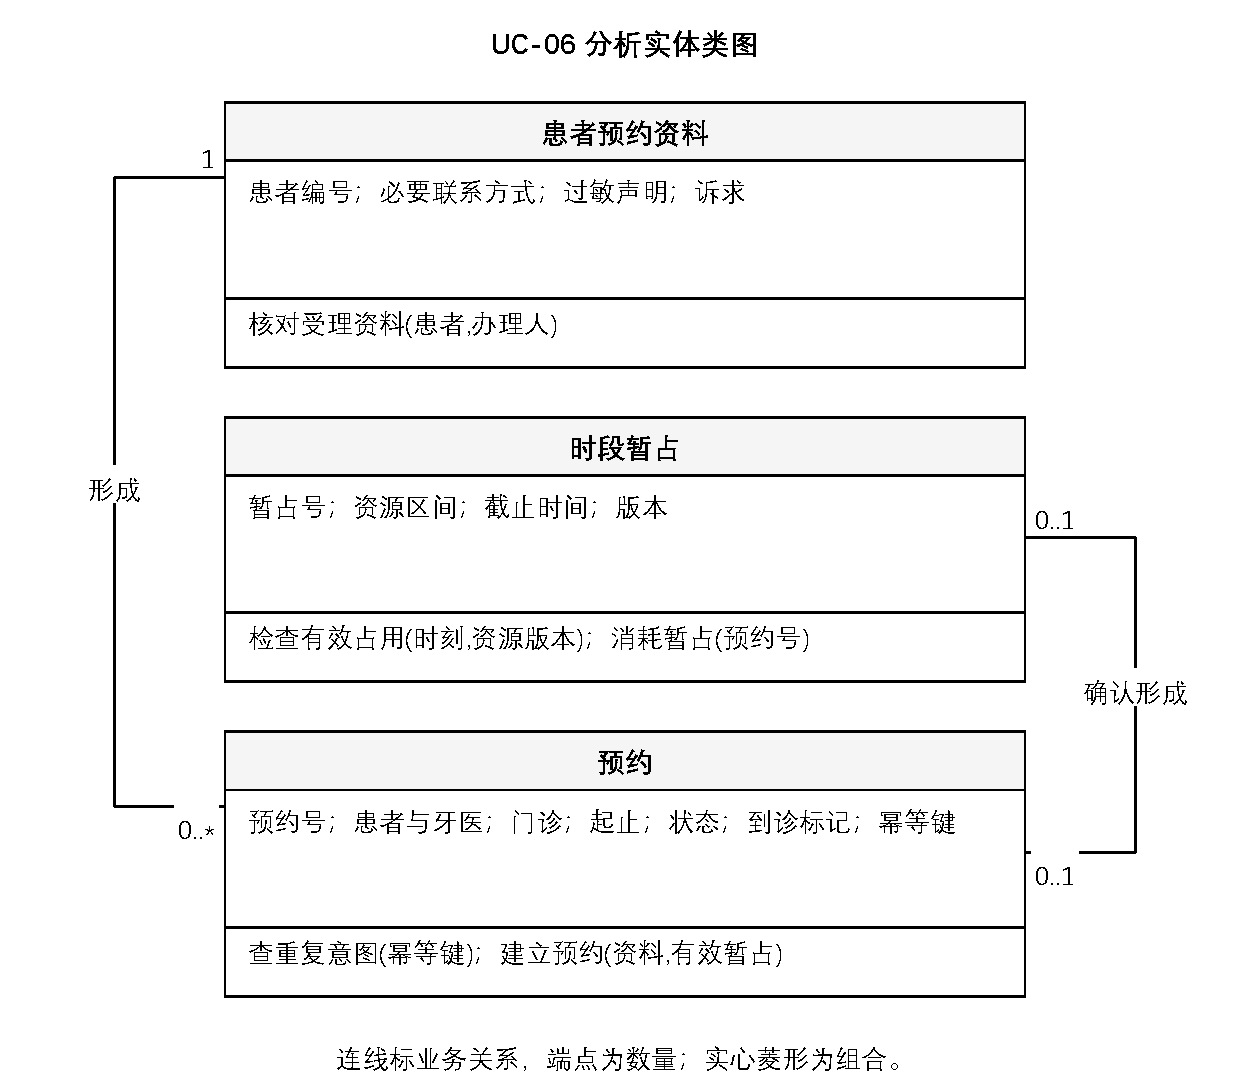
\includegraphics[width=\textwidth]{figures/class_UC_06.pdf}
\caption{UC-06 分析实体类图}\label{class_UC_06}\end{figure}
\begin{figure}[H]\centering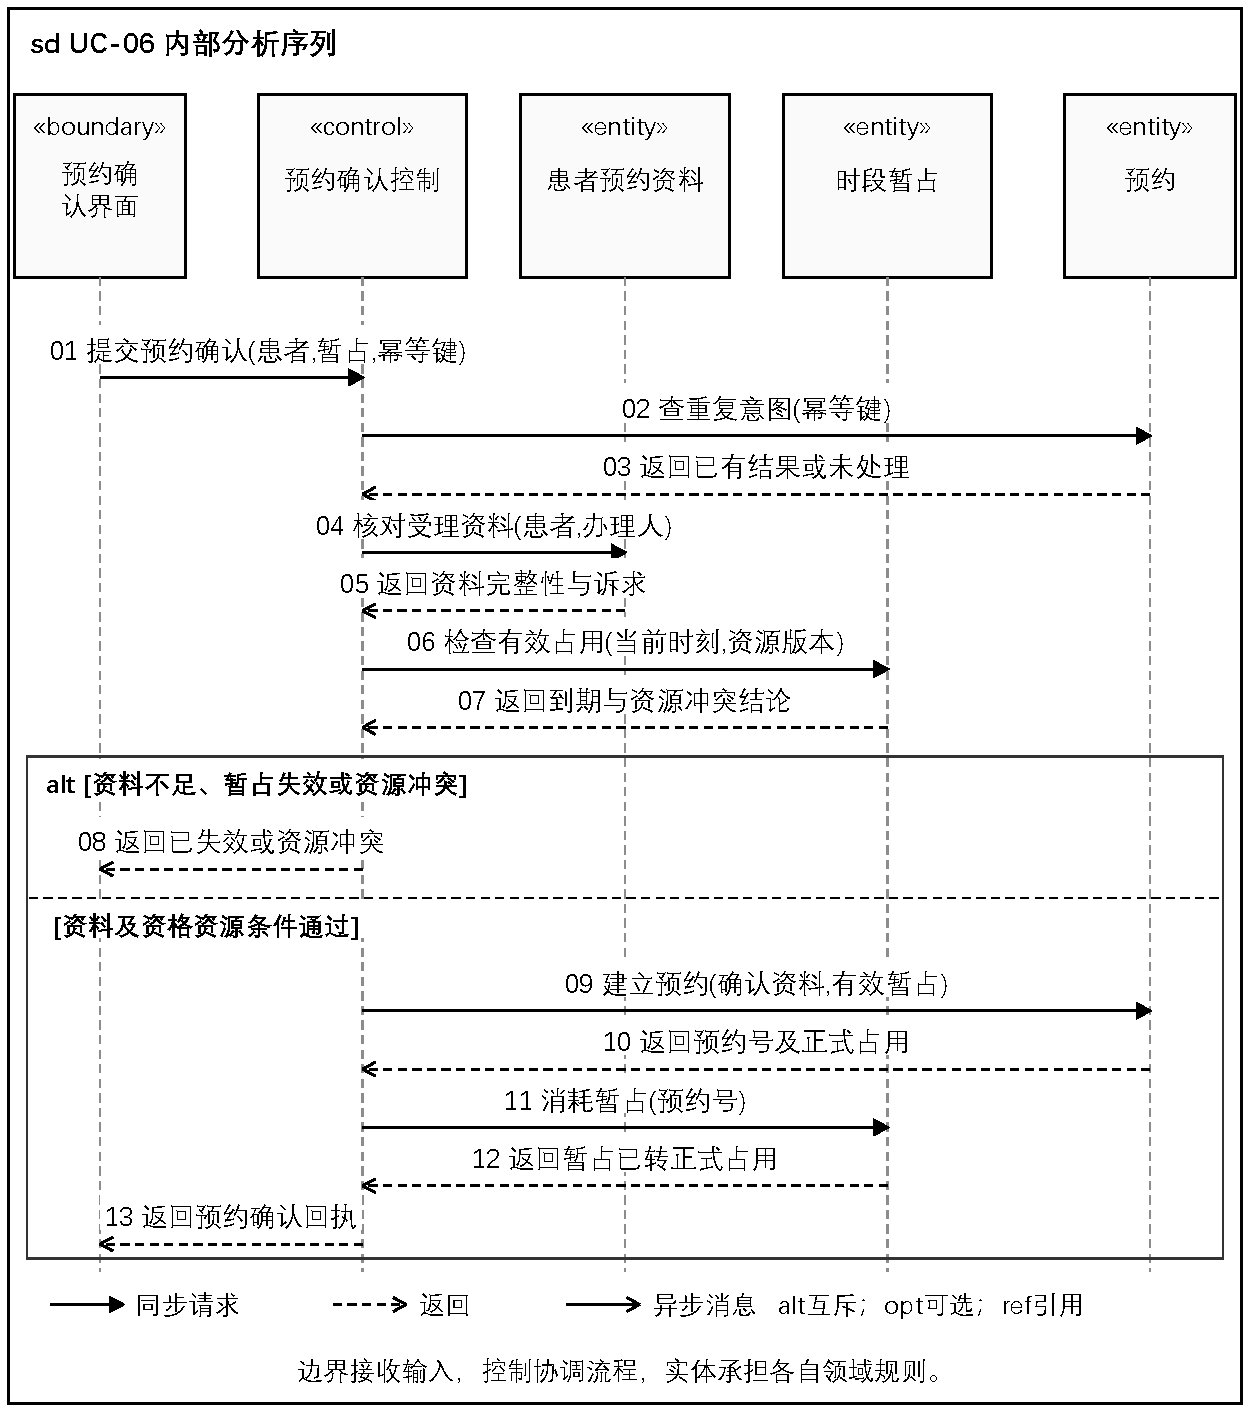
\includegraphics[width=\textwidth]{figures/seq_UC_06.pdf}
\caption{UC-06 内部分析序列}\label{seq_UC_06}\end{figure}
\par\noindent\begin{minipage}{\textwidth}
{\fontsize{10.5pt}{13.2pt}\selectfont\setlength{\tabcolsep}{0pt}\renewcommand{\arraystretch}{1.08}
\captionof{table}{UC-06操作契约}\label{tab254}
\begin{tabular}{@{}p{2.640cm}@{\hspace{0.16cm}}p{12.640cm}@{}}
\toprule
\bfseries \Cell{项目} & \bfseries \Cell{详细设计}\\\midrule
\Cell{签名} & \Cell{confirm\allowbreak{}Appointment(\allowbreak{}command,\allowbreak{} idempotency\allowbreak{}Key,\allowbreak{} actor)\allowbreak{}}\\[1pt]
\Cell{输入} & \Cell{占位标识、占位版本、患者确认、规则确认和幂等键；患者与资源由服务端核验。}\\[1pt]
\Cell{执行前检查} & \Cell{本人或有效代约权限；必要资料已确认；暂占未到期}\\[1pt]
\Cell{成功结果} & \Cell{预约与正式资源占用同时成立，暂占已消耗，到诊状态为待登记。}\\[1pt]
\Cell{领域算法} & \Cell{先按幂等键查询已处理结果；按固定顺序锁定资源及暂占，重查资格和区间冲突，建立预约与占用并保存回执}\\[1pt]
\Cell{数据访问} & \Cell{预约仓储与统一资源占用表配合：booking\_\allowbreak{}holds记录占位，appointments保存预约，resource\_\allowbreak{}reservations约束资源区间，command\_\allowbreak{}receipts保存请求与结果。}\\[1pt]
\Cell{事务与并发} & \Cell{一个短事务写预约、占用、暂占状态和提醒发件记录；外部通知在提交后处理}\\[1pt]
\Cell{失败及恢复} & \Cell{SLOT\_\allowbreak{}UNAVAILABLE返回重选；HOLD\_\allowbreak{}EXPIRED提示重新选择；同键不同请求体返回REQUEST\_\allowbreak{}KEY\_\allowbreak{}REUSED。}\\[1pt]
\bottomrule\end{tabular}
}\end{minipage}\par\vspace{6pt}
\par\noindent\begin{minipage}{\textwidth}
{\fontsize{10.5pt}{13.2pt}\selectfont\setlength{\tabcolsep}{0pt}\renewcommand{\arraystretch}{1.08}
\captionof{table}{UC-06表示与验收}\label{tab255}
\begin{tabular}{@{}p{2.640cm}@{\hspace{0.16cm}}p{12.640cm}@{}}
\toprule
\bfseries \Cell{项目} & \bfseries \Cell{设计}\\\midrule
\Cell{界面} & \Cell{确认页显示患者姓名、医生、门诊地址、准确时段和暂占倒计时；成功页以可查询预约号证明成立。}\\[1pt]
\Cell{接口} & \Cell{POST /\allowbreak{}booking-\allowbreak{}holds 取得临时占位；POST /\allowbreak{}appointments/\allowbreak{}confirm 携带 hold\allowbreak{}Id、hold\allowbreak{}Version 和 Idempotency-\allowbreak{}Key 确认；GET /\allowbreak{}appointments/\allowbreak{}\{id\} 查询结果。}\\[1pt]
\Cell{验收场景} & \Cell{1.\allowbreak{} 顾客与前台同时确认同资源→仅一个预约成立。\\2.\allowbreak{} 同键重试十次→返回同一预约号。\\3.\allowbreak{} 回执通知失败→预约仍有效且前台出现待联系任务。}\\[1pt]
\bottomrule\end{tabular}
}\end{minipage}\par\vspace{6pt}
\Needspace{497pt}
\subsubsection{UC-07 改期或取消预约}
边界：预约变更界面；控制：预约变更控制。\par
\begin{figure}[H]\centering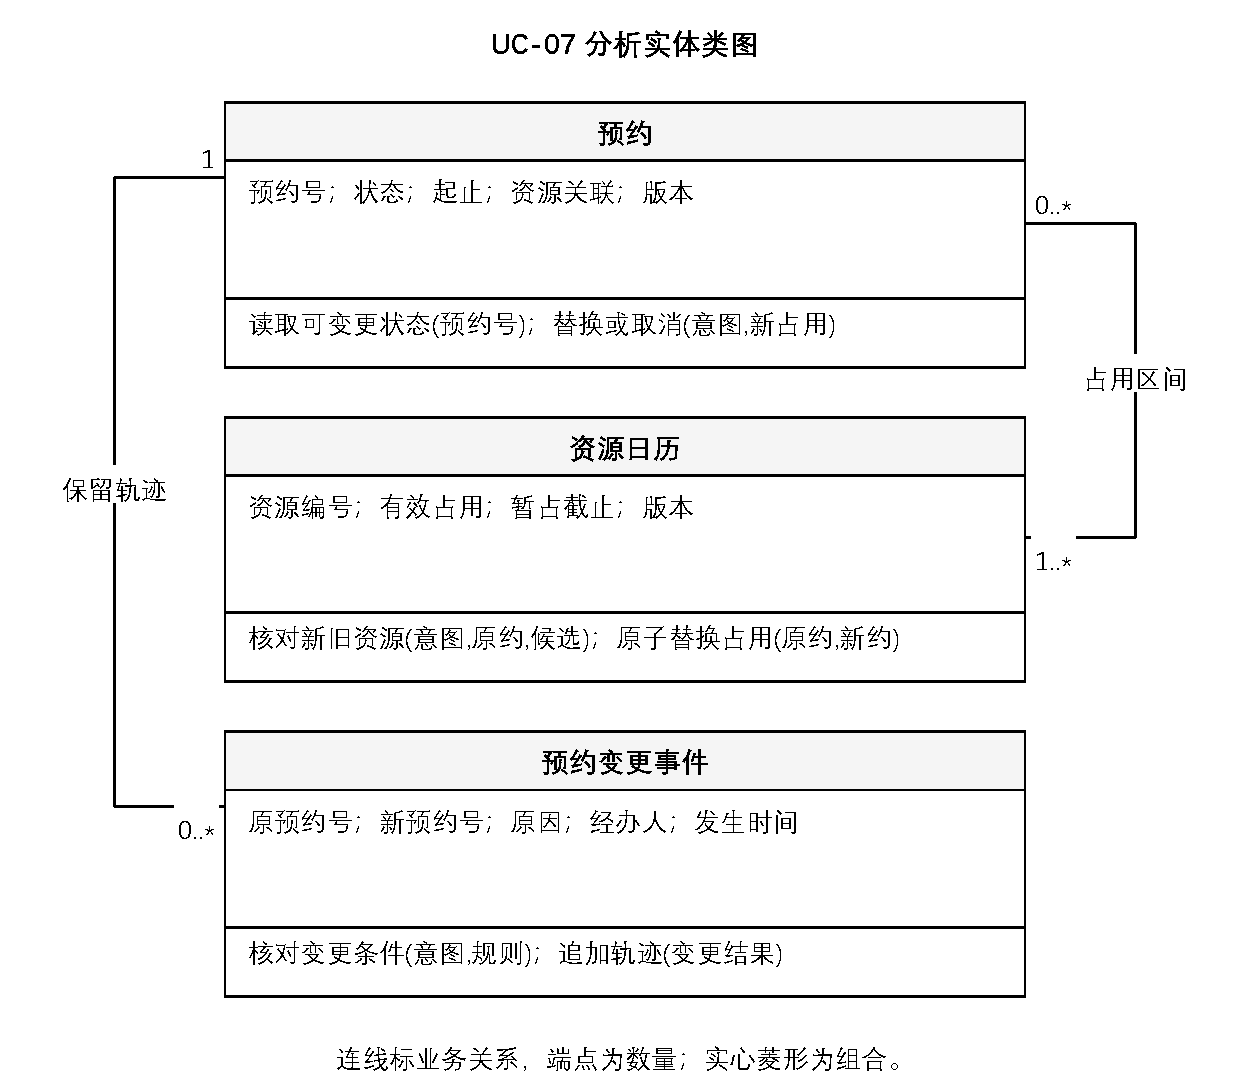
\includegraphics[width=\textwidth]{figures/class_UC_07.pdf}
\caption{UC-07 分析实体类图}\label{class_UC_07}\end{figure}
\begin{figure}[H]\centering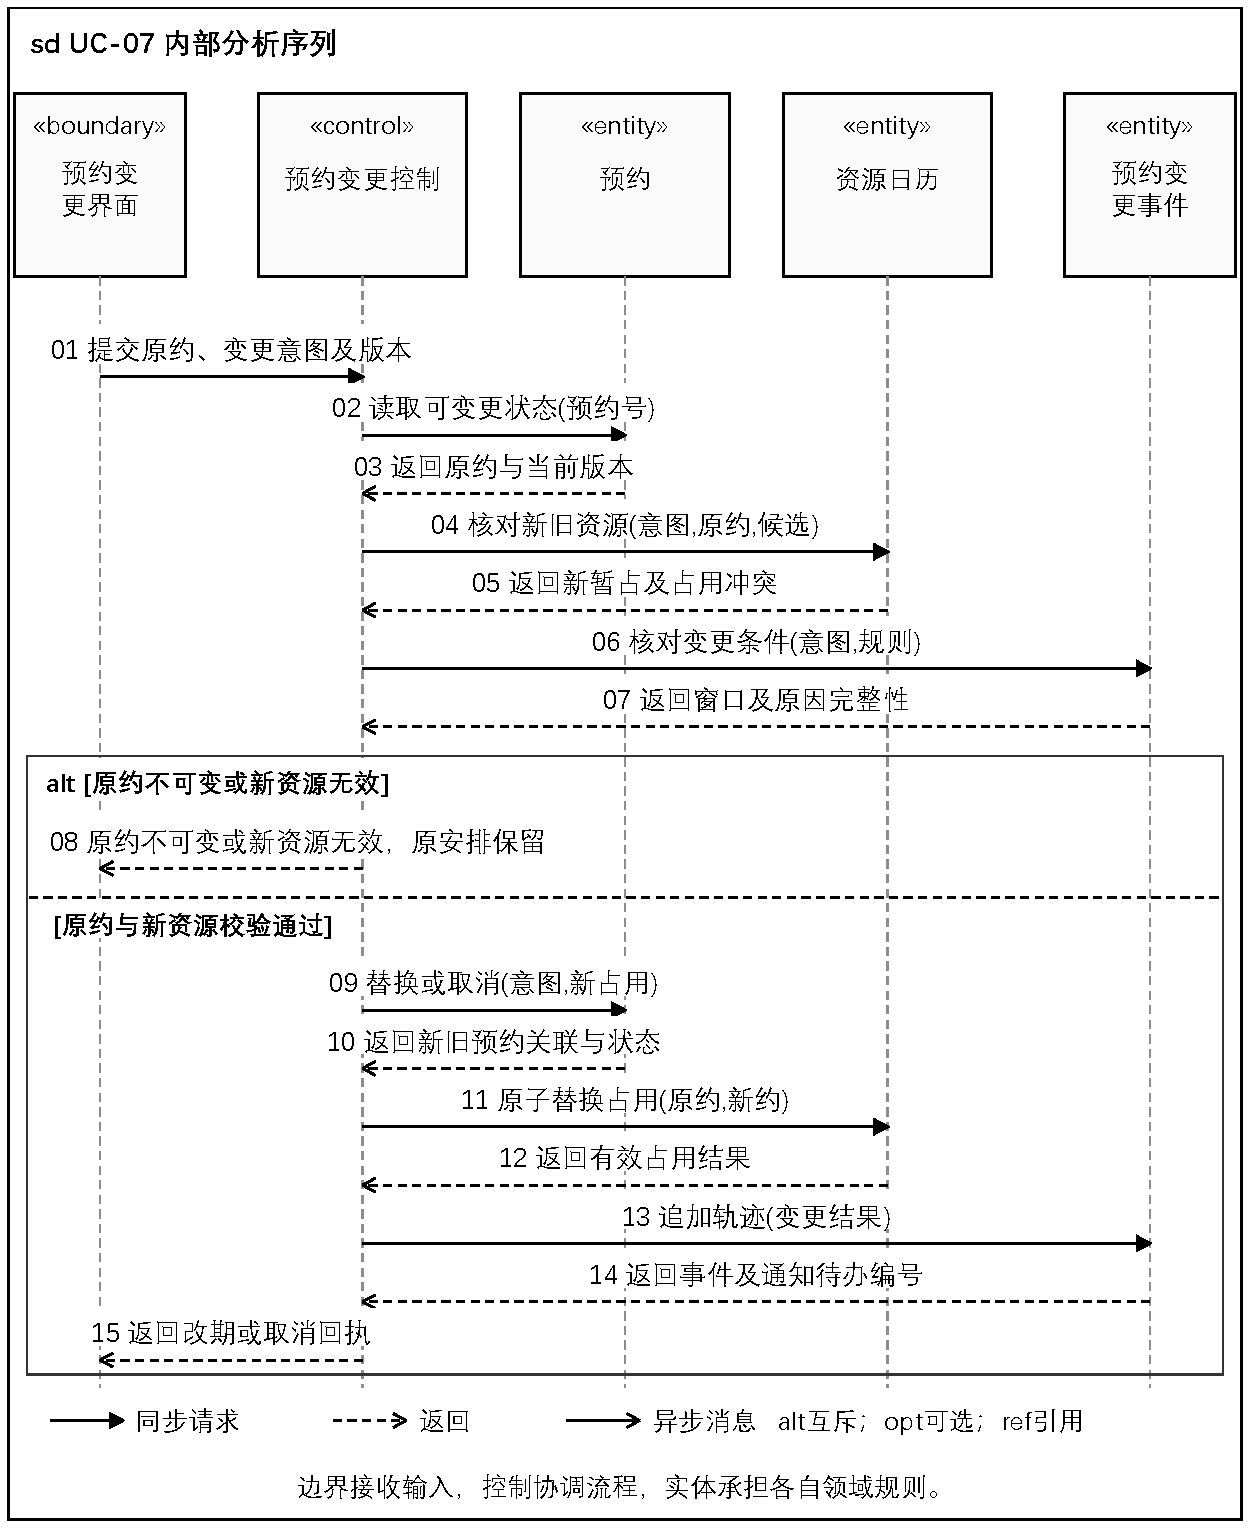
\includegraphics[width=\textwidth]{figures/seq_UC_07.pdf}
\caption{UC-07 内部分析序列}\label{seq_UC_07}\end{figure}
\par\noindent\begin{minipage}{\textwidth}
{\fontsize{10.5pt}{13.2pt}\selectfont\setlength{\tabcolsep}{0pt}\renewcommand{\arraystretch}{1.08}
\captionof{table}{UC-07操作契约}\label{tab260}
\begin{tabular}{@{}p{2.640cm}@{\hspace{0.16cm}}p{12.640cm}@{}}
\toprule
\bfseries \Cell{项目} & \bfseries \Cell{详细设计}\\\midrule
\Cell{签名} & \Cell{change\allowbreak{}Appointment(\allowbreak{}id,\allowbreak{} intent,\allowbreak{} hold\allowbreak{}Id,\allowbreak{} hold\allowbreak{}Version,\allowbreak{} reason,\allowbreak{} expected\allowbreak{}Version,\allowbreak{} request\allowbreak{}Key)\allowbreak{}}\\[1pt]
\Cell{输入} & \Cell{原预约、变更类型、原因、原预约版本和幂等键；改期另需有效的新占位标识和版本。}\\[1pt]
\Cell{执行前检查} & \Cell{本人或代约权限；原约可变更；人工例外有确认依据}\\[1pt]
\Cell{成功结果} & \Cell{预约、资源和事件一致，失败时原约保持}\\[1pt]
\Cell{领域算法} & \Cell{按固定顺序锁定新旧资源并重读原约；取消释放占用；改期建立新约及前后关联，再切换资源；写变更事件和通知任务}\\[1pt]
\Cell{数据访问} & \Cell{预约仓储装载原预约及资源占用；appointment\_\allowbreak{}events保存变更原因和操作事件，新旧预约保留关联，旧预约不删除。}\\[1pt]
\Cell{事务与并发} & \Cell{单事务替换预约与资源、写事件；异常整体回滚；外部通知提交后处理}\\[1pt]
\Cell{失败及恢复} & \Cell{VERSION\_\allowbreak{}CONFLICT显示新状态；目标占位失效或冲突时保留原约，相关诊疗流程按其业务状态处理。}\\[1pt]
\bottomrule\end{tabular}
}\end{minipage}\par\vspace{6pt}
\par\noindent\begin{minipage}{\textwidth}
{\fontsize{10.5pt}{13.2pt}\selectfont\setlength{\tabcolsep}{0pt}\renewcommand{\arraystretch}{1.08}
\captionof{table}{UC-07表示与验收}\label{tab261}
\begin{tabular}{@{}p{2.640cm}@{\hspace{0.16cm}}p{12.640cm}@{}}
\toprule
\bfseries \Cell{项目} & \bfseries \Cell{设计}\\\midrule
\Cell{界面} & \Cell{改期页同时显示原安排与新安排；取消需确认原因，提交后单独展示退款等后续事项状态。}\\[1pt]
\Cell{接口} & \Cell{改期先通过 POST /\allowbreak{}booking-\allowbreak{}holds 取得新占位；POST /\allowbreak{}appointments/\allowbreak{}\{id\}/\allowbreak{}changes 携带 intent、reason、expected\allowbreak{}Version 和 Idempotency-\allowbreak{}Key，改期另传 hold\allowbreak{}Id、hold\allowbreak{}Version。}\\[1pt]
\Cell{验收场景} & \Cell{1.\allowbreak{} 抢新时段失败→旧约仍可查询且占用不变。\\2.\allowbreak{} 取消重复请求→一个取消事件、一次资源释放。\\3.\allowbreak{} 已开始接诊后取消→拒绝且保留实际就诊。}\\[1pt]
\bottomrule\end{tabular}
}\end{minipage}\par\vspace{6pt}
\Needspace{497pt}
\subsubsection{UC-08 发送提醒并处理候补邀请}
边界：提醒候补工作台；控制：联系任务控制。\par
\begin{figure}[H]\centering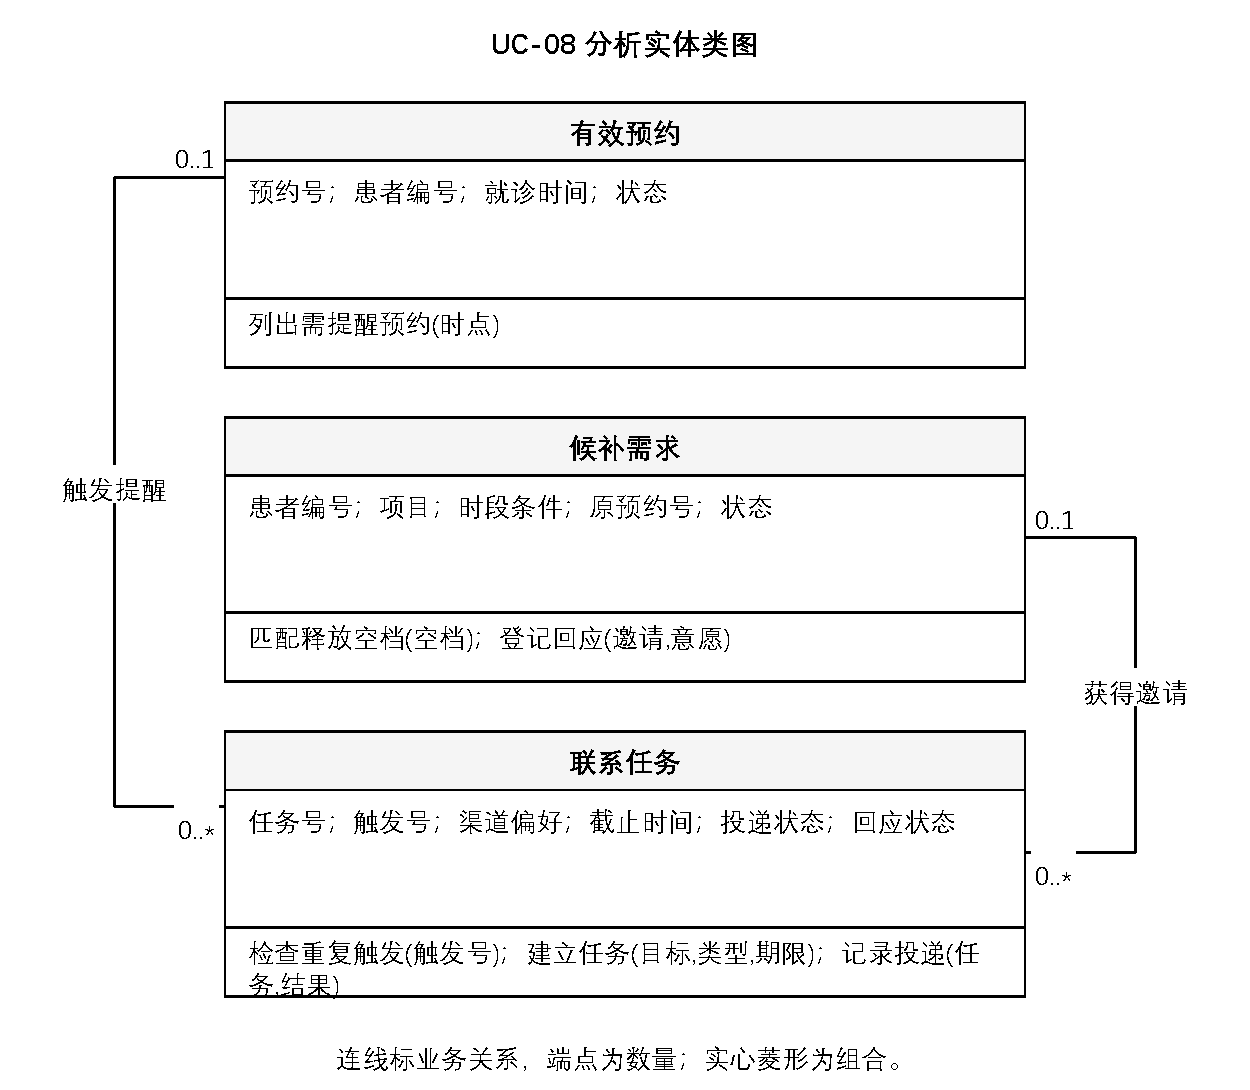
\includegraphics[width=\textwidth]{figures/class_UC_08.pdf}
\caption{UC-08 分析实体类图}\label{class_UC_08}\end{figure}
\begin{figure}[H]\centering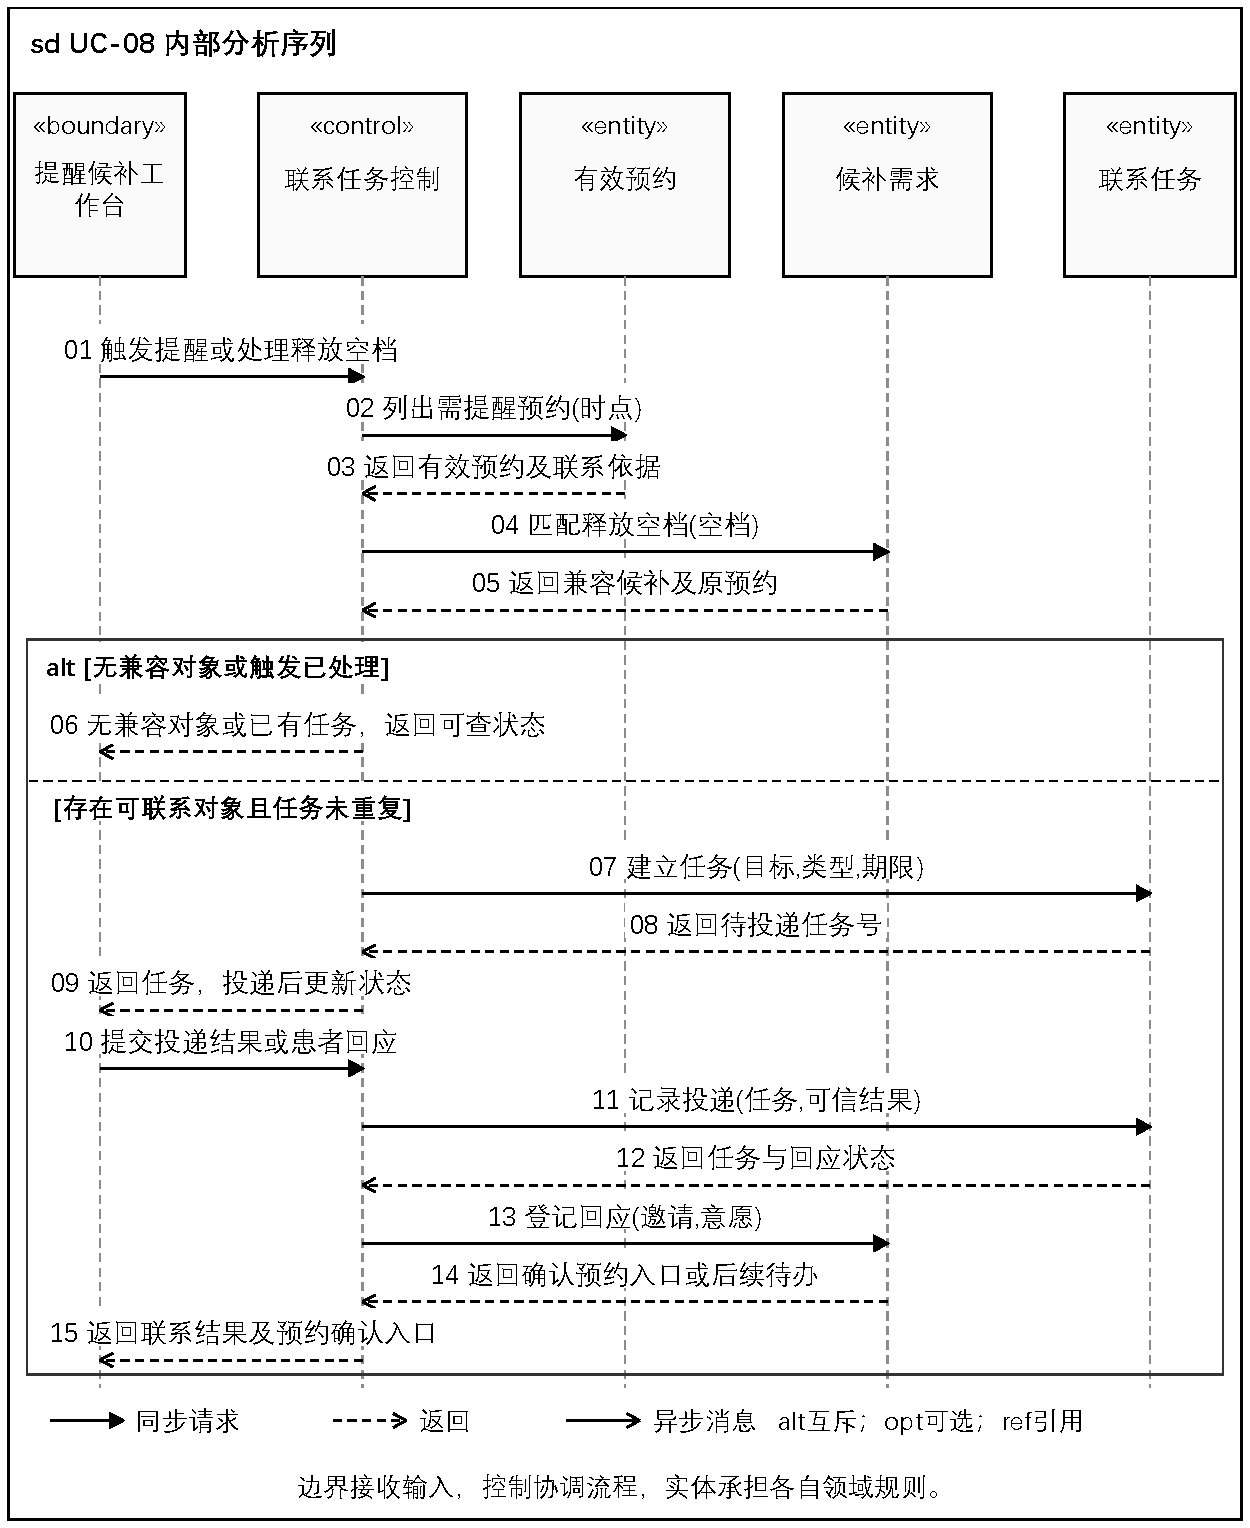
\includegraphics[width=\textwidth]{figures/seq_UC_08.pdf}
\caption{UC-08 内部分析序列}\label{seq_UC_08}\end{figure}
\par\noindent\begin{minipage}{\textwidth}
{\fontsize{10.5pt}{13.2pt}\selectfont\setlength{\tabcolsep}{0pt}\renewcommand{\arraystretch}{1.08}
\captionof{table}{UC-08操作契约}\label{tab266}
\begin{tabular}{@{}p{2.640cm}@{\hspace{0.16cm}}p{12.640cm}@{}}
\toprule
\bfseries \Cell{项目} & \bfseries \Cell{详细设计}\\\midrule
\Cell{签名} & \Cell{create\allowbreak{}Contact\allowbreak{}Task(\allowbreak{}trigger\allowbreak{}Id,\allowbreak{} type,\allowbreak{} target,\allowbreak{} expires\allowbreak{}At)\allowbreak{}}\\[1pt]
\Cell{输入} & \Cell{提醒时点或释放事件、目标患者和邀请截止}\\[1pt]
\Cell{执行前检查} & \Cell{有效预约或兼容候补存在；联系偏好允许}\\[1pt]
\Cell{成功结果} & \Cell{建立唯一任务及待投递事件，不改变预约成立状态}\\[1pt]
\Cell{领域算法} & \Cell{按触发编号查重，读取联系偏好并匹配条件；生成受控内容和期限；工作器调用通知适配器后回写真实结果}\\[1pt]
\Cell{数据访问} & \Cell{Contact\allowbreak{}Task\allowbreak{}Repository与Waitlist\allowbreak{}Repository；notification\_\allowbreak{}tasks保存每个业务触发的任务及投递状态，投递变化追加audit\_\allowbreak{}events；waitlist\_\allowbreak{}entries保存候补邀请与回应，dedupe\_\allowbreak{}key防重复任务。}\\[1pt]
\Cell{事务与并发} & \Cell{任务及发件记录一起提交；外部投递另行执行；回执按任务锁定去重}\\[1pt]
\Cell{失败及恢复} & \Cell{PREFERENCE\_\allowbreak{}BLOCKED转人工合法渠道；DELIVERY\_\allowbreak{}UNKNOWN等待查询；INVITATION\_\allowbreak{}EXPIRED不调用预约确认}\\[1pt]
\bottomrule\end{tabular}
}\end{minipage}\par\vspace{6pt}
\par\noindent\begin{minipage}{\textwidth}
{\fontsize{10.5pt}{13.2pt}\selectfont\setlength{\tabcolsep}{0pt}\renewcommand{\arraystretch}{1.08}
\captionof{table}{UC-08表示与验收}\label{tab267}
\begin{tabular}{@{}p{2.640cm}@{\hspace{0.16cm}}p{12.640cm}@{}}
\toprule
\bfseries \Cell{项目} & \bfseries \Cell{设计}\\\midrule
\Cell{界面} & \Cell{工作台分别列出未发送、失败和未回应；患者消息展示地点、时间及操作入口，候补入口注明确认条件。}\\[1pt]
\Cell{接口} & \Cell{POST /\allowbreak{}contact-\allowbreak{}tasks；POST /\allowbreak{}waitlist-\allowbreak{}invitations/\allowbreak{}\{id\}/\allowbreak{}responses；回执入口校验来源与事件唯一号。}\\[1pt]
\Cell{验收场景} & \Cell{1.\allowbreak{} 重复释放事件→同一患者不重复收到同轮邀请。\\2.\allowbreak{} 接收消息后空档已占→回应保留且预约未成立。\\3.\allowbreak{} 发送接口受理但未送达→界面保持已发送，不显示已送达。}\\[1pt]
\bottomrule\end{tabular}
}\end{minipage}\par\vspace{6pt}
\Needspace{497pt}
\subsubsection{UC-09 办理到诊并确认未到情况}
边界：到诊接待界面；控制：到诊核实控制。\par
\begin{figure}[H]\centering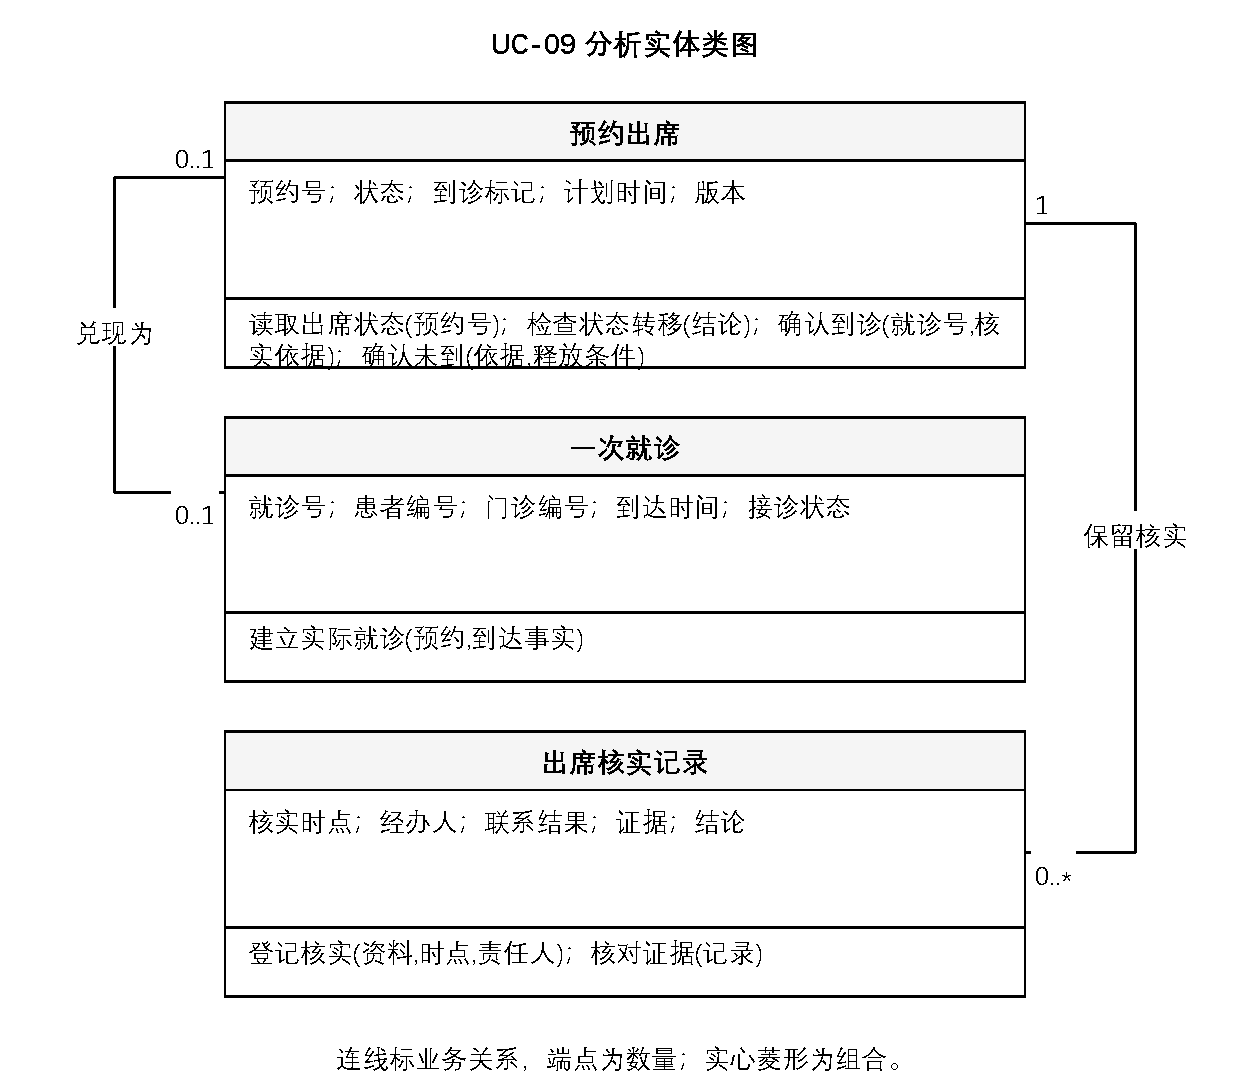
\includegraphics[width=\textwidth]{figures/class_UC_09.pdf}
\caption{UC-09 分析实体类图}\label{class_UC_09}\end{figure}
\begin{figure}[H]\centering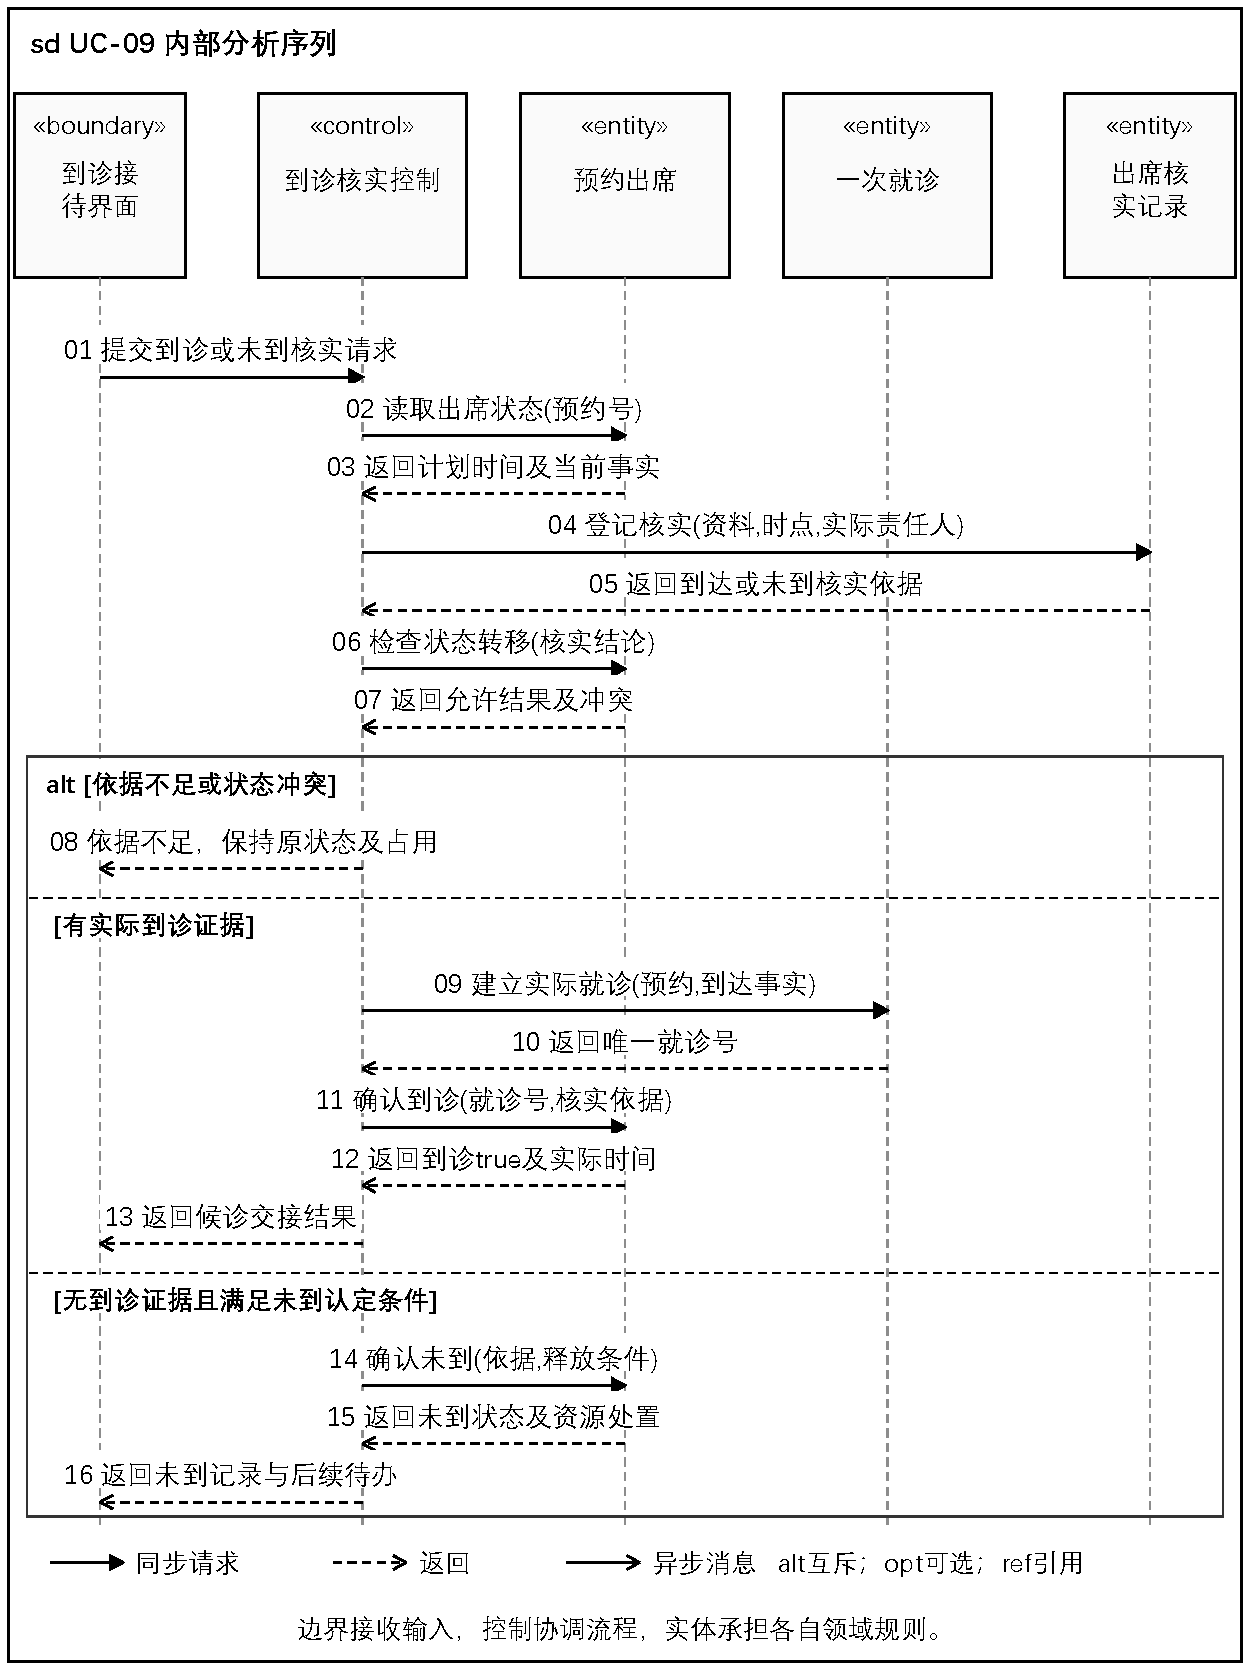
\includegraphics[width=\textwidth]{figures/seq_UC_09.pdf}
\caption{UC-09 内部分析序列}\label{seq_UC_09}\end{figure}
\par\noindent\begin{minipage}{\textwidth}
{\fontsize{10.5pt}{13.2pt}\selectfont\setlength{\tabcolsep}{0pt}\renewcommand{\arraystretch}{1.08}
\captionof{table}{UC-09操作契约}\label{tab272}
\begin{tabular}{@{}p{2.640cm}@{\hspace{0.16cm}}p{12.640cm}@{}}
\toprule
\bfseries \Cell{项目} & \bfseries \Cell{详细设计}\\\midrule
\Cell{签名} & \Cell{record\allowbreak{}Attendance(\allowbreak{}appointment\allowbreak{}Id,\allowbreak{} conclusion,\allowbreak{} evidence,\allowbreak{} expected\allowbreak{}Version)\allowbreak{}}\\[1pt]
\Cell{输入} & \Cell{预约号、到达或联系依据、实际时间和处理结论}\\[1pt]
\Cell{执行前检查} & \Cell{本店接待任务有效；未到满足核实及释放条件}\\[1pt]
\Cell{成功结果} & \Cell{到诊只对应一个实际就诊，未到及资源处理有核实记录}\\[1pt]
\Cell{领域算法} & \Cell{锁定预约并读已存在就诊；重复到诊返回原号；实际到诊写encounter及true，未到写独立状态；追加事实事件与核实依据}\\[1pt]
\Cell{数据访问} & \Cell{Attendance\allowbreak{}Repository与Encounter\allowbreak{}Repository；appointments.\allowbreak{}attended、visits、appointment\_\allowbreak{}events，预约到有效就诊唯一}\\[1pt]
\Cell{事务与并发} & \Cell{预约、就诊、核实事件及释放占用同一事务；不在此事务改账单或收入}\\[1pt]
\Cell{失败及恢复} & \Cell{EVIDENCE\_\allowbreak{}PENDING保留状态；ALREADY\_\allowbreak{}ARRIVED返回原就诊；STATE\_\allowbreak{}CONFLICT交有权人员更正}\\[1pt]
\bottomrule\end{tabular}
}\end{minipage}\par\vspace{6pt}
\par\noindent\begin{minipage}{\textwidth}
{\fontsize{10.5pt}{13.2pt}\selectfont\setlength{\tabcolsep}{0pt}\renewcommand{\arraystretch}{1.08}
\captionof{table}{UC-09表示与验收}\label{tab273}
\begin{tabular}{@{}p{2.640cm}@{\hspace{0.16cm}}p{12.640cm}@{}}
\toprule
\bfseries \Cell{项目} & \bfseries \Cell{设计}\\\midrule
\Cell{界面} & \Cell{到诊与未到分列操作，默认展示待核实；迟到输入实际时间和协调意见，不自动缩短治疗。}\\[1pt]
\Cell{接口} & \Cell{POST /\allowbreak{}appointments/\allowbreak{}\{id\}/\allowbreak{}attendance；POST /\allowbreak{}attendance-\allowbreak{}events/\allowbreak{}\{id\}/\allowbreak{}corrections。更正带证据、理由与版本。}\\[1pt]
\Cell{验收场景} & \Cell{1.\allowbreak{} 预约尚未到时且attended=\allowbreak{}false→不计取消或未到。\\2.\allowbreak{} 两个签到请求→一个实际就诊。\\3.\allowbreak{} 联系不到但未到阈值未满足→保留原资源占用。}\\[1pt]
\bottomrule\end{tabular}
}\end{minipage}\par\vspace{6pt}
\Needspace{608pt}
\subsubsection{UC-10 接诊检查并制定治疗计划}
边界：医生接诊界面；控制：接诊计划控制。\par
\begin{figure}[H]\centering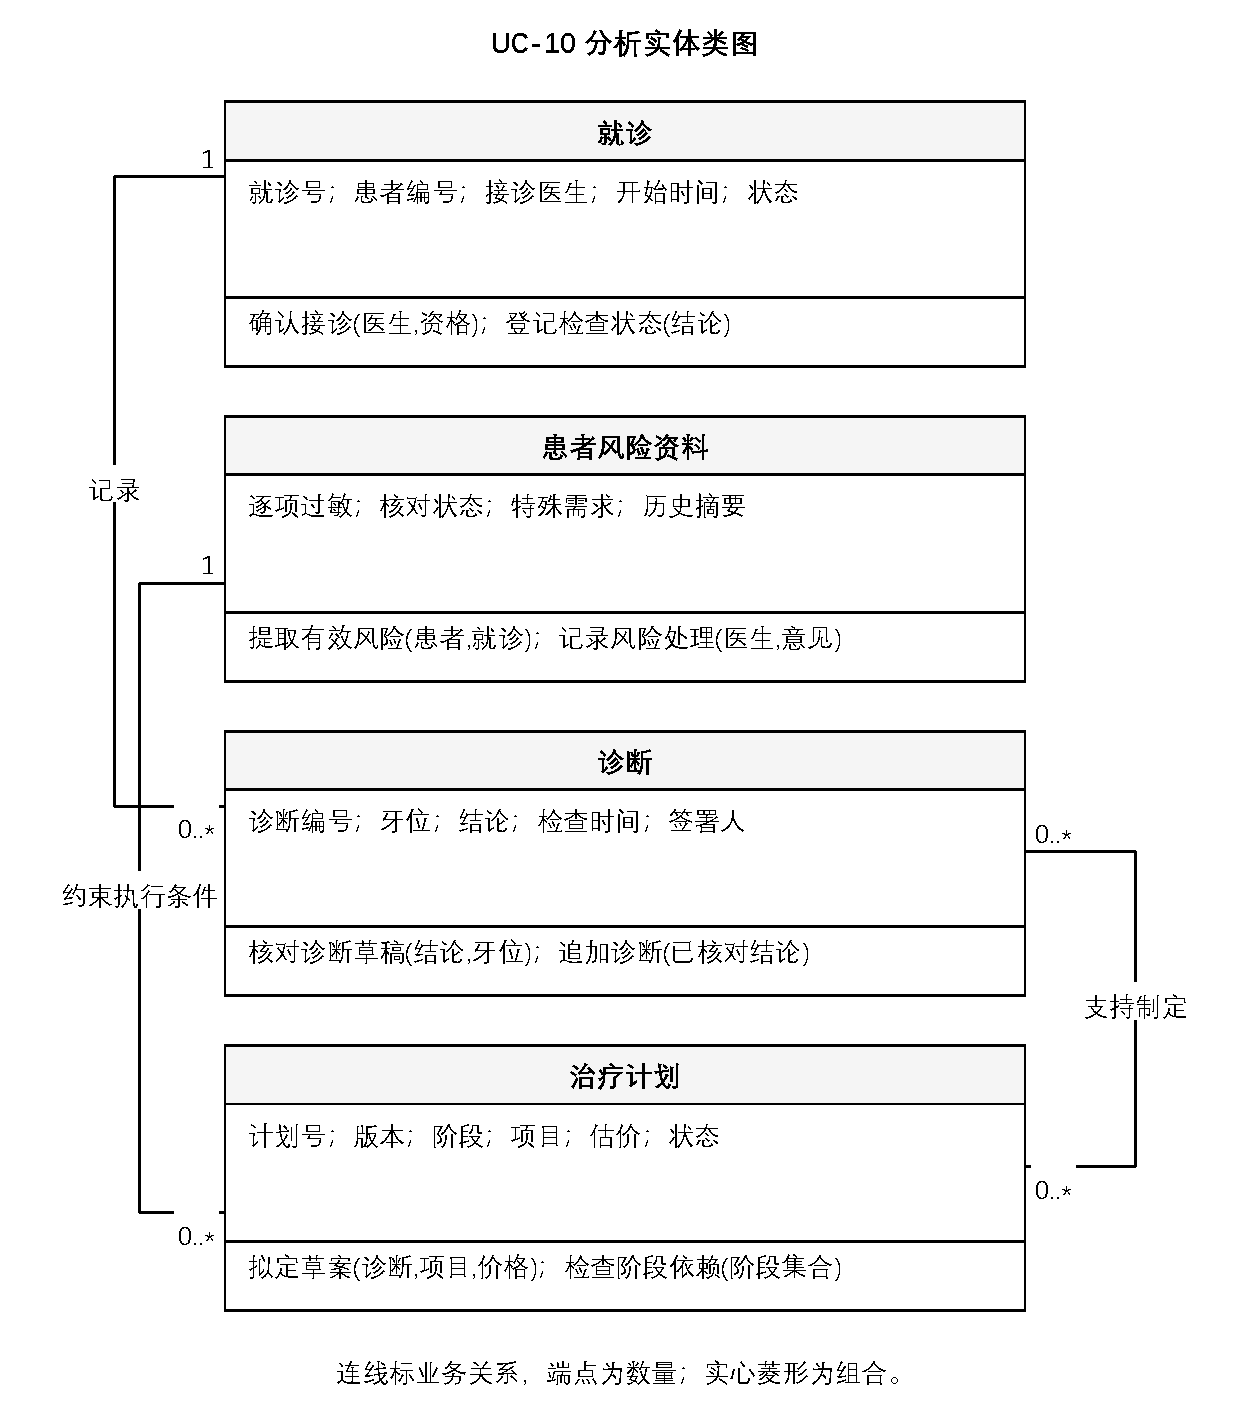
\includegraphics[width=\textwidth]{figures/class_UC_10.pdf}
\caption{UC-10 分析实体类图}\label{class_UC_10}\end{figure}
\begin{figure}[H]\centering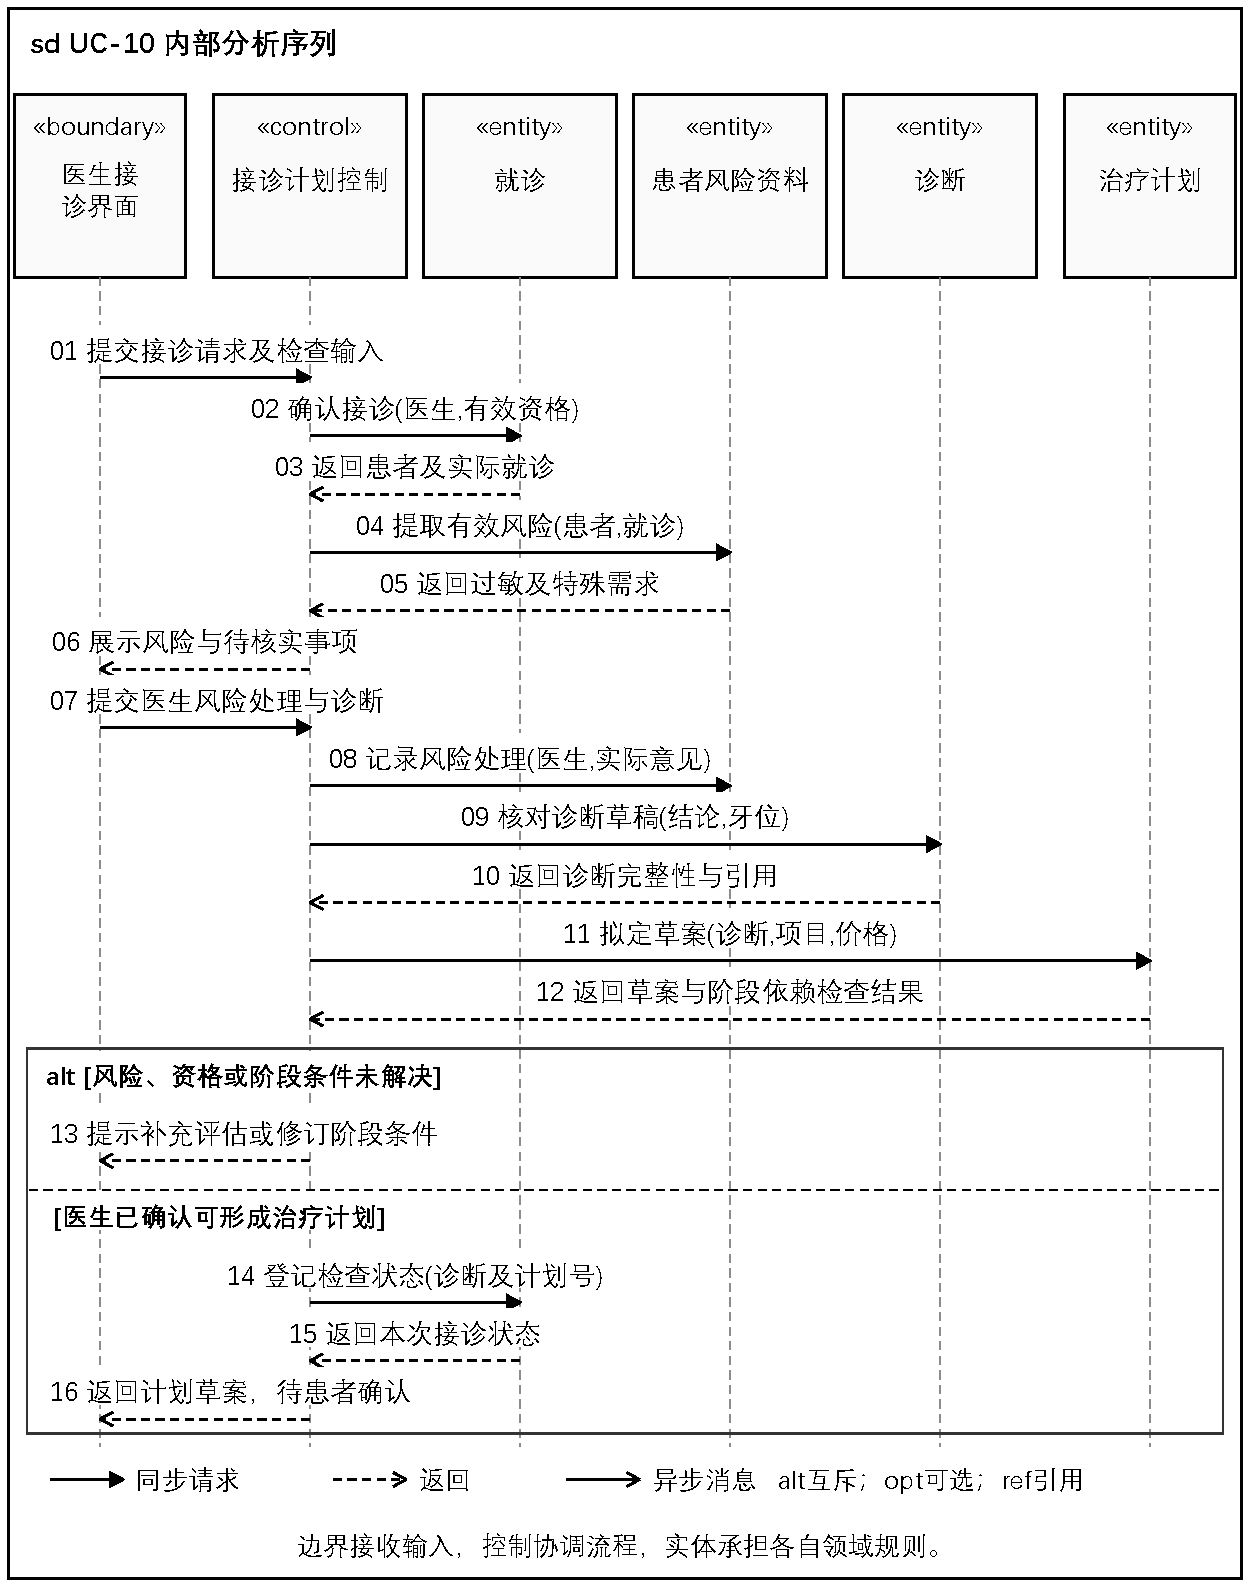
\includegraphics[width=\textwidth]{figures/seq_UC_10.pdf}
\caption{UC-10 内部分析序列}\label{seq_UC_10}\end{figure}
\par\noindent\begin{minipage}{\textwidth}
{\fontsize{10.5pt}{13.2pt}\selectfont\setlength{\tabcolsep}{0pt}\renewcommand{\arraystretch}{1.08}
\captionof{table}{UC-10操作契约}\label{tab278}
\begin{tabular}{@{}p{2.640cm}@{\hspace{0.16cm}}p{12.640cm}@{}}
\toprule
\bfseries \Cell{项目} & \bfseries \Cell{详细设计}\\\midrule
\Cell{签名} & \Cell{draft\allowbreak{}Treatment\allowbreak{}Plan(\allowbreak{}encounter\allowbreak{}Id,\allowbreak{} assessment,\allowbreak{} stages,\allowbreak{} items,\allowbreak{} expected\allowbreak{}Version)\allowbreak{}}\\[1pt]
\Cell{输入} & \Cell{检查结论、过敏处理、特殊需求、阶段及计划项目}\\[1pt]
\Cell{执行前检查} & \Cell{有本次接诊资格；已核对患者及风险资料}\\[1pt]
\Cell{成功结果} & \Cell{诊断及计划草案可追溯，依赖无环，未确认项目不可执行}\\[1pt]
\Cell{领域算法} & \Cell{核对医生接诊任务及风险处理；将诊断与牙位关联就诊；按项目取有效价目快照；拓扑检查阶段依赖，保存新草案版本}\\[1pt]
\Cell{数据访问} & \Cell{Encounter\allowbreak{}Repository、Clinical\allowbreak{}Record\allowbreak{}Repository与Treatment\allowbreak{}Plan\allowbreak{}Repository；diagnoses、treatment\_\allowbreak{}plans、plan\_\allowbreak{}versions、plan\_\allowbreak{}items、plan\_\allowbreak{}items}\\[1pt]
\Cell{事务与并发} & \Cell{诊断草案及计划版本同事务提交；已签诊断用附记，不覆盖原文；历史资料只读}\\[1pt]
\Cell{失败及恢复} & \Cell{RISK\_\allowbreak{}UNRESOLVED保留评估；QUALIFICATION\_\allowbreak{}MISMATCH安排合格医生；DEPENDENCY\_\allowbreak{}CYCLE阻止发布}\\[1pt]
\bottomrule\end{tabular}
}\end{minipage}\par\vspace{6pt}
\par\noindent\begin{minipage}{\textwidth}
{\fontsize{10.5pt}{13.2pt}\selectfont\setlength{\tabcolsep}{0pt}\renewcommand{\arraystretch}{1.08}
\captionof{table}{UC-10表示与验收}\label{tab279}
\begin{tabular}{@{}p{2.640cm}@{\hspace{0.16cm}}p{12.640cm}@{}}
\toprule
\bfseries \Cell{项目} & \bfseries \Cell{设计}\\\midrule
\Cell{界面} & \Cell{医生工作台先显示患者及风险，随后记录诊断和阶段；费用估计明显标识，患者确认状态单独显示。}\\[1pt]
\Cell{接口} & \Cell{POST /\allowbreak{}visits/\allowbreak{}\{id\}/\allowbreak{}assessments；POST /\allowbreak{}treatment-\allowbreak{}plans；POST /\allowbreak{}treatment-\allowbreak{}plans/\allowbreak{}\{id\}/\allowbreak{}versions。签署人由会话及资格确定。}\\[1pt]
\Cell{验收场景} & \Cell{1.\allowbreak{} 患者有乳胶过敏但未核对→执行放行受阻并保留评估。\\2.\allowbreak{} 阶段A依赖B且B依赖A→返回循环路径。\\3.\allowbreak{} 患者跨店复诊→可在授权范围沿用原计划。}\\[1pt]
\bottomrule\end{tabular}
}\end{minipage}\par\vspace{6pt}
\Needspace{497pt}
\subsubsection{UC-11 确认方案及治疗增项}
边界：方案确认界面；控制：方案签认控制。\par
\begin{figure}[H]\centering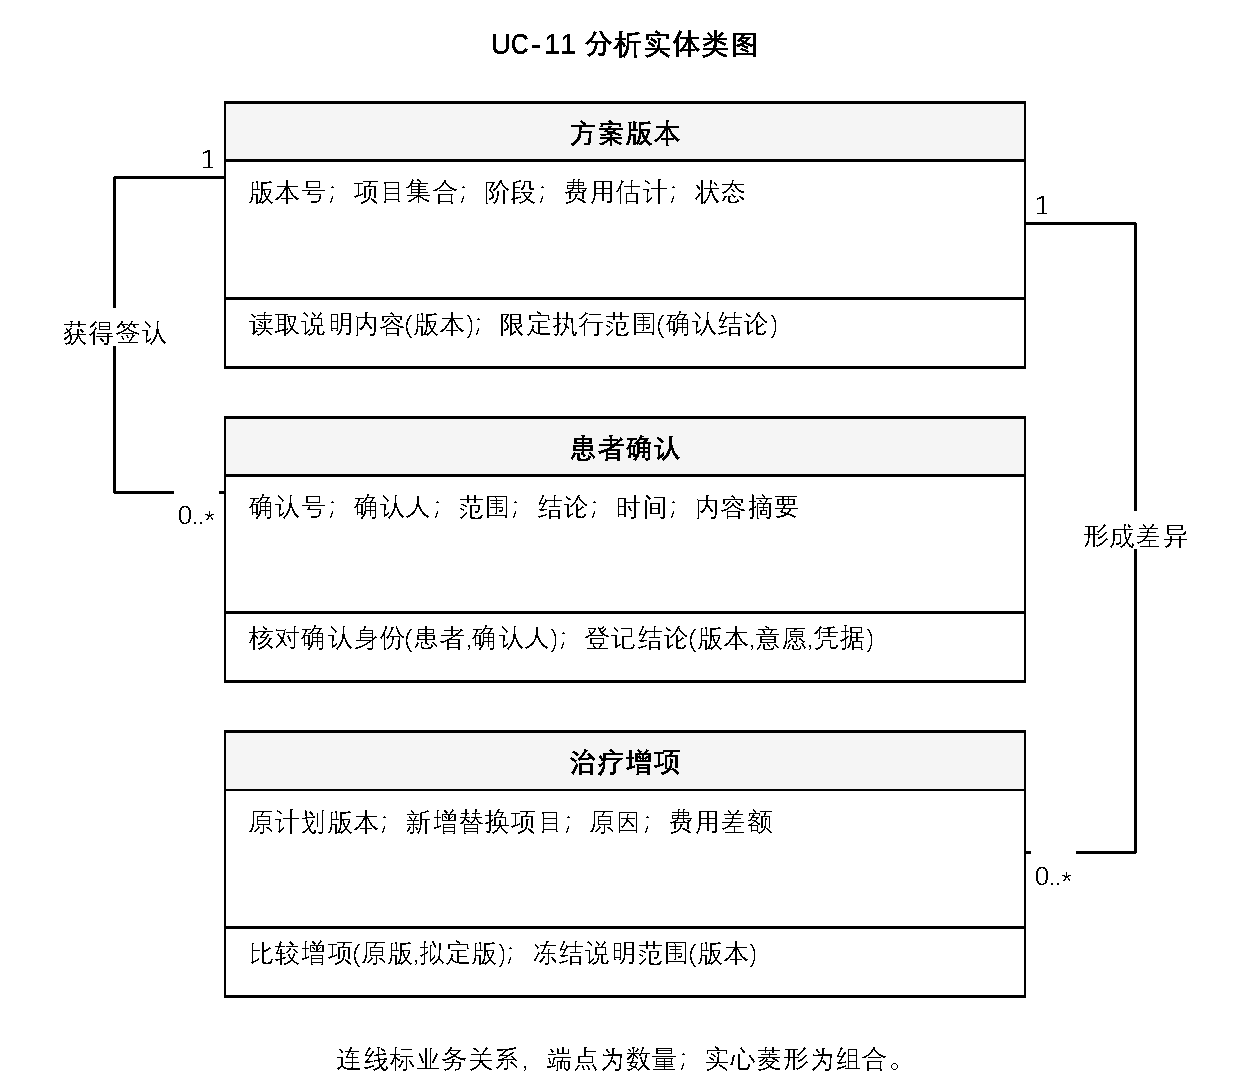
\includegraphics[width=\textwidth]{figures/class_UC_11.pdf}
\caption{UC-11 分析实体类图}\label{class_UC_11}\end{figure}
\begin{figure}[H]\centering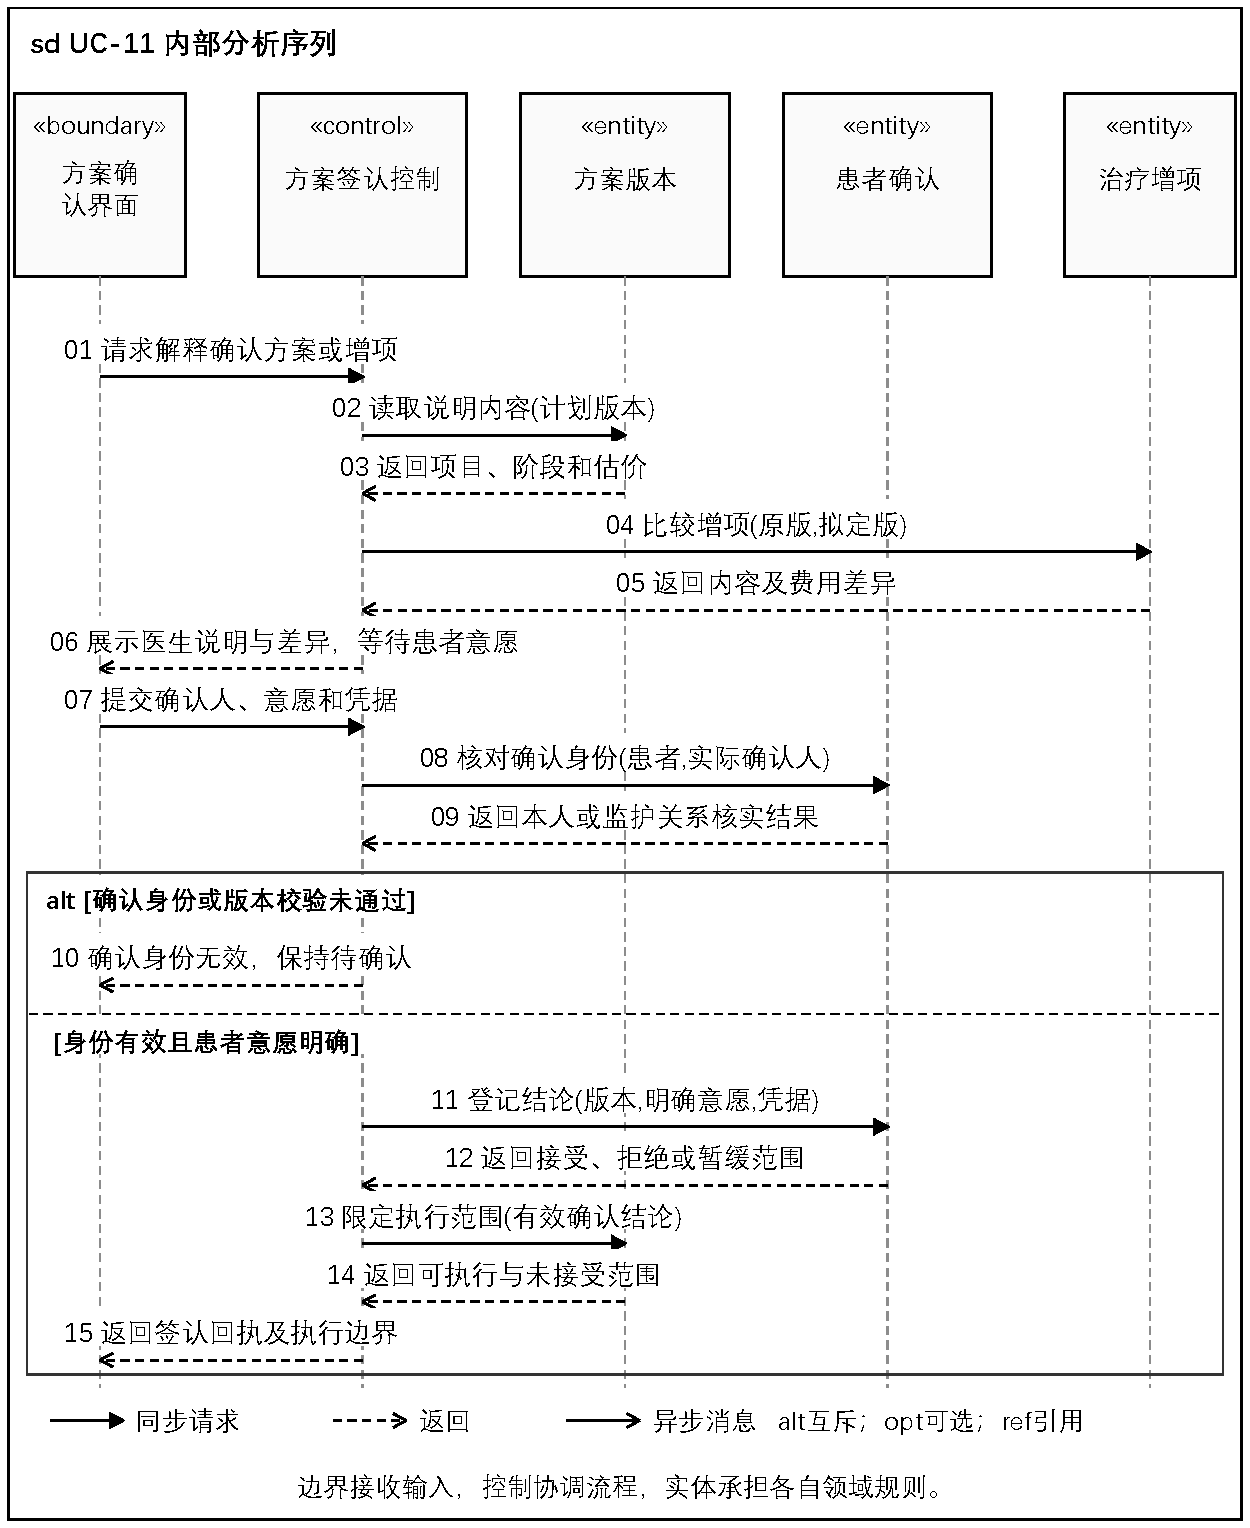
\includegraphics[width=\textwidth]{figures/seq_UC_11.pdf}
\caption{UC-11 内部分析序列}\label{seq_UC_11}\end{figure}
\par\noindent\begin{minipage}{\textwidth}
{\fontsize{10.5pt}{13.2pt}\selectfont\setlength{\tabcolsep}{0pt}\renewcommand{\arraystretch}{1.08}
\captionof{table}{UC-11操作契约}\label{tab284}
\begin{tabular}{@{}p{2.640cm}@{\hspace{0.16cm}}p{12.640cm}@{}}
\toprule
\bfseries \Cell{项目} & \bfseries \Cell{详细设计}\\\midrule
\Cell{签名} & \Cell{confirm\allowbreak{}Treatment\allowbreak{}Scope(\allowbreak{}plan\allowbreak{}Version\allowbreak{}Id,\allowbreak{} decision,\allowbreak{} scope,\allowbreak{} signer,\allowbreak{} evidence,\allowbreak{} request\allowbreak{}Key)\allowbreak{}}\\[1pt]
\Cell{输入} & \Cell{具体版本及项目、确认结论、确认人身份、说明与签认凭据}\\[1pt]
\Cell{执行前检查} & \Cell{确认身份有效；专业说明完成；计划版本未被替代}\\[1pt]
\Cell{成功结果} & \Cell{签认与具体内容绑定；只将接受范围标为可执行}\\[1pt]
\Cell{领域算法} & \Cell{按版本比对增项并重算估价；核对确认人或监护关系；固定内容摘要与意愿；只放行已接受项目，拒绝和暂缓保留原因}\\[1pt]
\Cell{数据访问} & \Cell{Consent\allowbreak{}Repository与Treatment\allowbreak{}Plan\allowbreak{}Repository；consent\_\allowbreak{}records、consent\_\allowbreak{}items和plan\_\allowbreak{}versions，内容哈希及线下凭据受控存储}\\[1pt]
\Cell{事务与并发} & \Cell{锁定方案版本后写签认及可执行范围；版本变化整体拒绝；外部签名凭据先核验再提交引用}\\[1pt]
\Cell{失败及恢复} & \Cell{SIGNER\_\allowbreak{}INVALID保持待确认；PLAN\_\allowbreak{}SUPERSEDED展示新版；SCOPE\_\allowbreak{}MISMATCH重新说明}\\[1pt]
\bottomrule\end{tabular}
}\end{minipage}\par\vspace{6pt}
\par\noindent\begin{minipage}{\textwidth}
{\fontsize{10.5pt}{13.2pt}\selectfont\setlength{\tabcolsep}{0pt}\renewcommand{\arraystretch}{1.08}
\captionof{table}{UC-11表示与验收}\label{tab285}
\begin{tabular}{@{}p{2.640cm}@{\hspace{0.16cm}}p{12.640cm}@{}}
\toprule
\bfseries \Cell{项目} & \bfseries \Cell{设计}\\\midrule
\Cell{界面} & \Cell{患者页逐项显示新增、保留和撤销内容及费用差额，提供接受、拒绝、暂缓；签认前显示实际确认人。}\\[1pt]
\Cell{接口} & \Cell{GET /\allowbreak{}plan-\allowbreak{}versions/\allowbreak{}\{id\}/\allowbreak{}explanation；POST /\allowbreak{}plan-\allowbreak{}versions/\allowbreak{}\{id\}/\allowbreak{}consents，带scope、decision、evidence\allowbreak{}Ref及幂等键。}\\[1pt]
\Cell{验收场景} & \Cell{1.\allowbreak{} 新增X光但未取得确认→执行接口拒绝该增项。\\2.\allowbreak{} 患者仅接受部分项目→只有对应项目获放行。\\3.\allowbreak{} 签认后目录改价→原确认费用快照不变。}\\[1pt]
\bottomrule\end{tabular}
}\end{minipage}\par\vspace{6pt}
\Needspace{608pt}
\subsubsection{UC-12 记录实际治疗与医疗用品耗用}
边界：治疗执行界面；控制：实际治疗控制。\par
\begin{figure}[H]\centering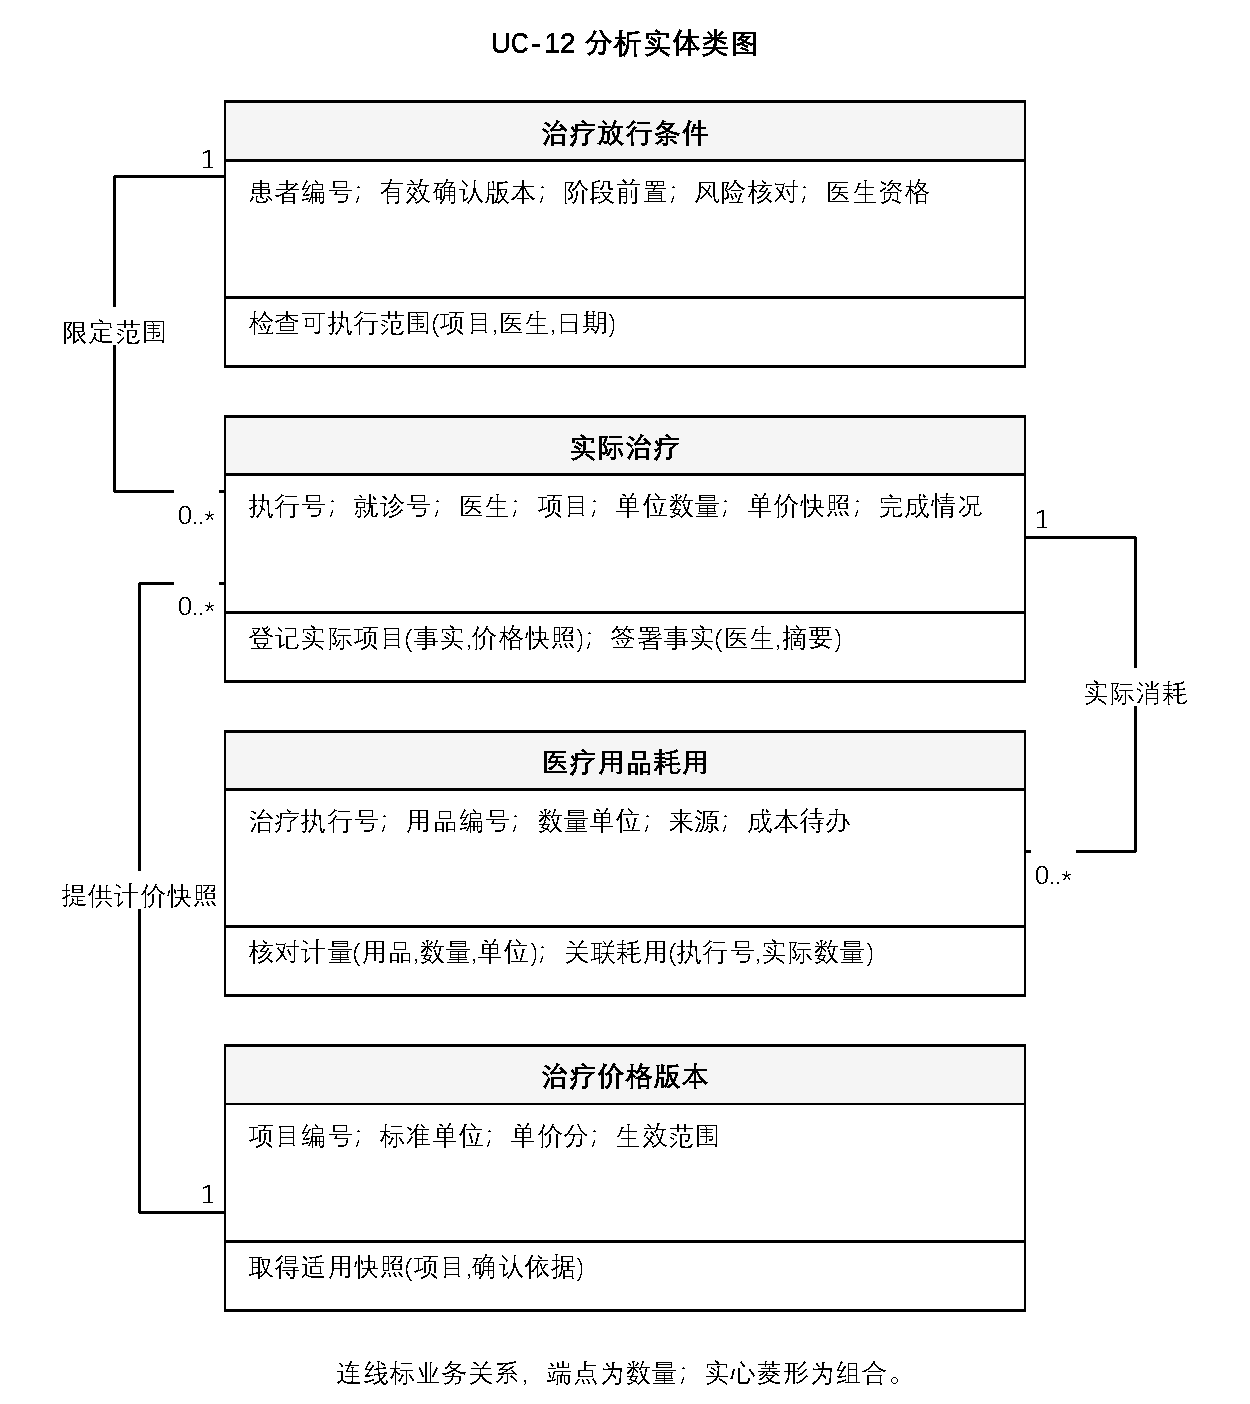
\includegraphics[width=\textwidth]{figures/class_UC_12.pdf}
\caption{UC-12 分析实体类图}\label{class_UC_12}\end{figure}
\begin{figure}[H]\centering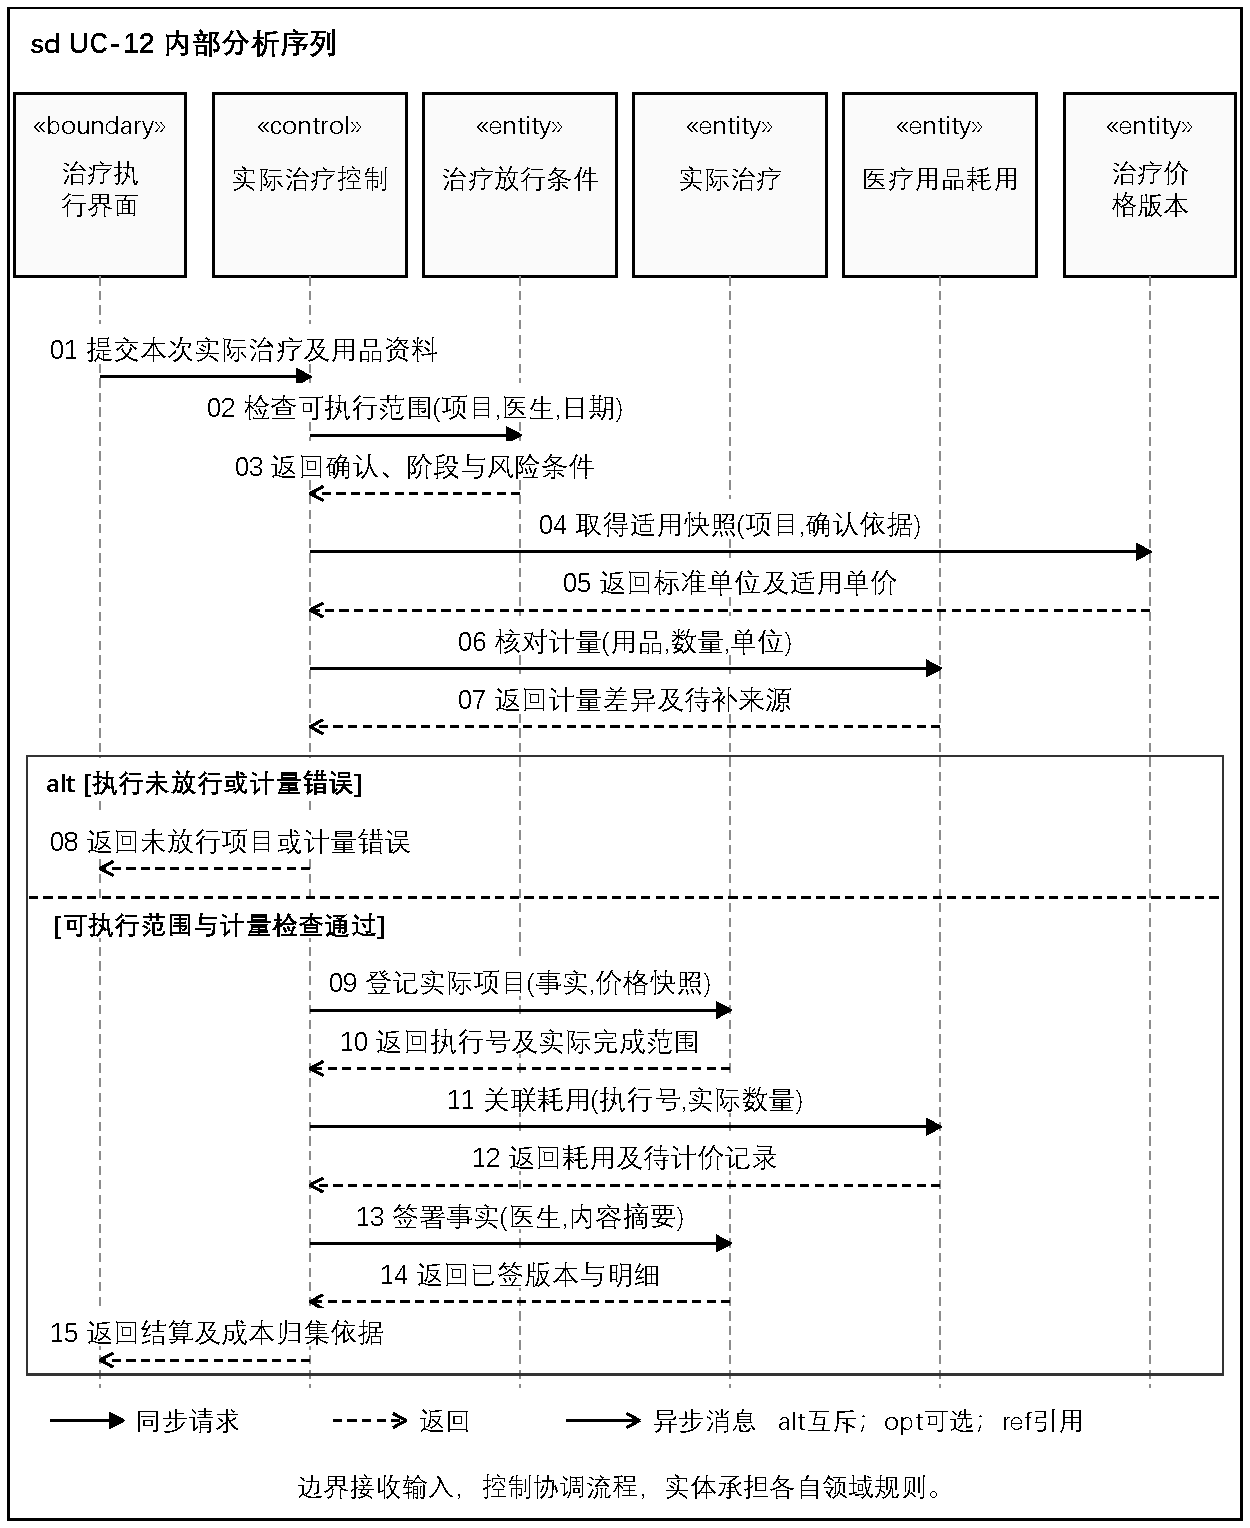
\includegraphics[width=\textwidth]{figures/seq_UC_12.pdf}
\caption{UC-12 内部分析序列}\label{seq_UC_12}\end{figure}
\par\noindent\begin{minipage}{\textwidth}
{\fontsize{10.5pt}{13.2pt}\selectfont\setlength{\tabcolsep}{0pt}\renewcommand{\arraystretch}{1.08}
\captionof{table}{UC-12操作契约}\label{tab290}
\begin{tabular}{@{}p{2.640cm}@{\hspace{0.16cm}}p{12.640cm}@{}}
\toprule
\bfseries \Cell{项目} & \bfseries \Cell{详细设计}\\\midrule
\Cell{签名} & \Cell{sign\allowbreak{}Treatment\allowbreak{}Execution(\allowbreak{}encounter\allowbreak{}Id,\allowbreak{} actual\allowbreak{}Items,\allowbreak{} materials,\allowbreak{} expected\allowbreak{}Version,\allowbreak{} request\allowbreak{}Key)\allowbreak{}}\\[1pt]
\Cell{输入} & \Cell{实际项目、牙位、单位数量、完成情况、适用价格及用品清单}\\[1pt]
\Cell{执行前检查} & \Cell{本次就诊医生任务与资格有效；具体项目已确认并满足阶段条件}\\[1pt]
\Cell{成功结果} & \Cell{签署执行与耗用关联一致，结算和成本只能引用这些事实}\\[1pt]
\Cell{领域算法} & \Cell{逐项检查风险及确认范围，取已说明价目快照；校验实际数量和耗用品单位；建立治疗执行及用品记录，计算签署摘要并固定版本}\\[1pt]
\Cell{数据访问} & \Cell{Treatment\allowbreak{}Execution\allowbreak{}Repository与Material\allowbreak{}Usage\allowbreak{}Repository；treatment\_\allowbreak{}executions、execution\_\allowbreak{}items、material\_\allowbreak{}consumptions，保存医生和门诊及price\_\allowbreak{}version\_\allowbreak{}id}\\[1pt]
\Cell{事务与并发} & \Cell{一个事务写执行、用品关联与签署；幂等号唯一；缺成本只建待补，不回滚已发生的医疗事实}\\[1pt]
\Cell{失败及恢复} & \Cell{SCOPE\_\allowbreak{}NOT\_\allowbreak{}CONFIRMED转\mbox{UC-11}；UNIT\_\allowbreak{}MISMATCH纠正计量；SIGNED\_\allowbreak{}IMMUTABLE要求附记更正}\\[1pt]
\bottomrule\end{tabular}
}\end{minipage}\par\vspace{6pt}
\par\noindent\begin{minipage}{\textwidth}
{\fontsize{10.5pt}{13.2pt}\selectfont\setlength{\tabcolsep}{0pt}\renewcommand{\arraystretch}{1.08}
\captionof{table}{UC-12表示与验收}\label{tab291}
\begin{tabular}{@{}p{2.640cm}@{\hspace{0.16cm}}p{12.640cm}@{}}
\toprule
\bfseries \Cell{项目} & \bfseries \Cell{设计}\\\midrule
\Cell{界面} & \Cell{按实际项目逐行填写数量与完成情况，旁显标准单位和价格；耗用品独立列表；签署前展示本次全部事实。}\\[1pt]
\Cell{接口} & \Cell{POST /\allowbreak{}visits/\allowbreak{}\{id\}/\allowbreak{}executions；POST /\allowbreak{}executions/\allowbreak{}\{id\}/\allowbreak{}signatures；POST /\allowbreak{}executions/\allowbreak{}\{id\}/\allowbreak{}addenda。签署校验医生本人及版本。}\\[1pt]
\Cell{验收场景} & \Cell{1.\allowbreak{} 计划3单位但实际仅做2单位→执行记录2，结算依据为2。\\2.\allowbreak{} 用品有数量但缺计价证据→保留耗用并标待归集。\\3.\allowbreak{} 签署后修改原数量→拒绝覆盖，允许有追溯的更正。}\\[1pt]
\bottomrule\end{tabular}
}\end{minipage}\par\vspace{6pt}
\Needspace{497pt}
\subsubsection{UC-13 签署病历并追加更正附记}
边界：病历签署页；控制：病历签署控制。\par
\begin{figure}[H]\centering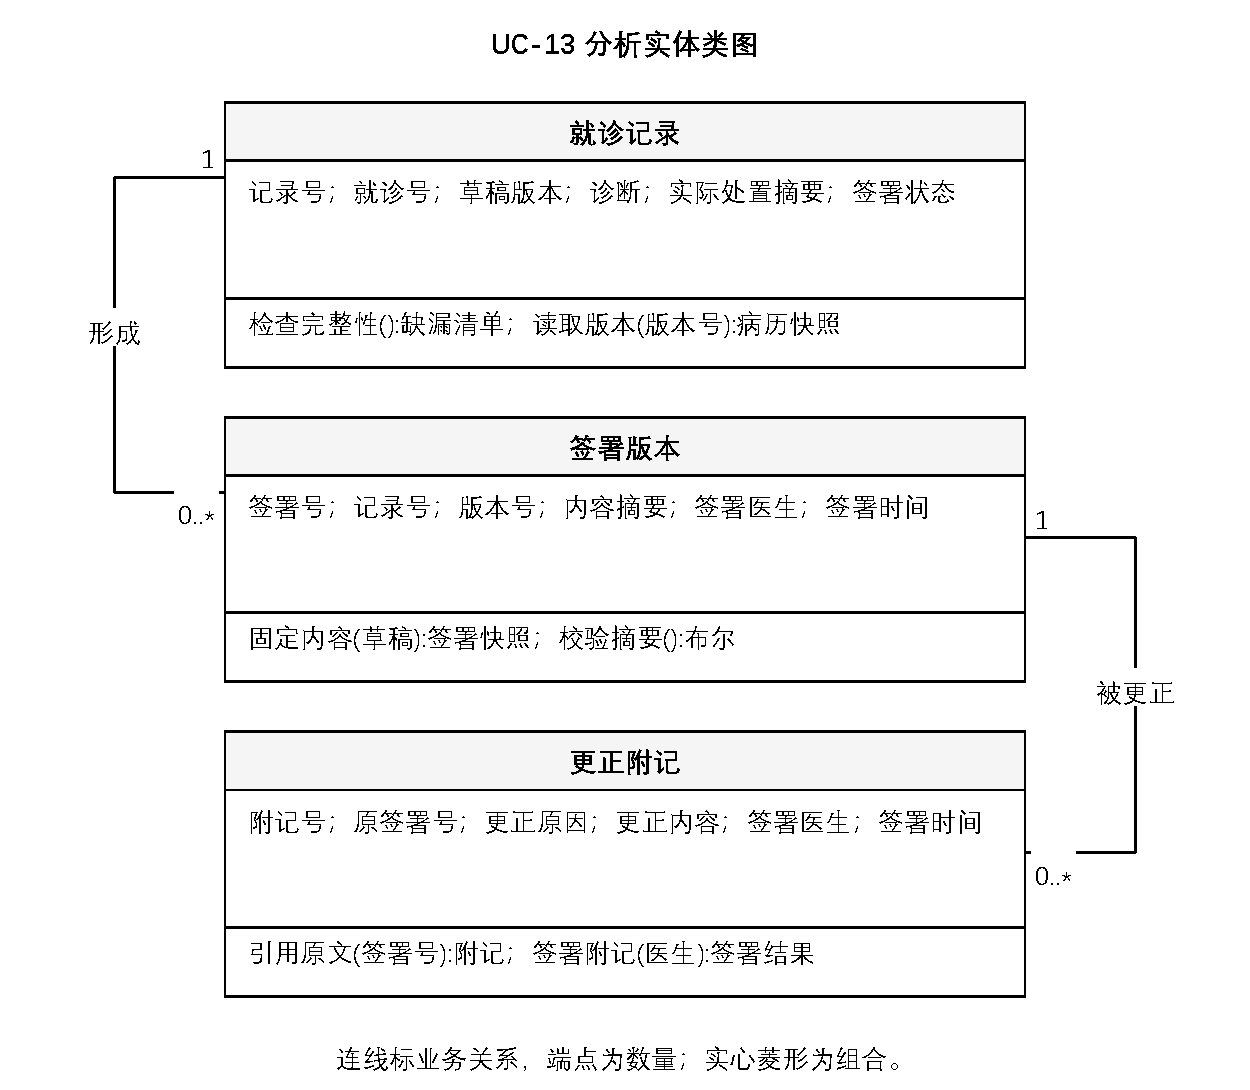
\includegraphics[width=\textwidth]{figures/class_UC_13.pdf}
\caption{UC-13 分析实体类图}\label{class_UC_13}\end{figure}
\begin{figure}[H]\centering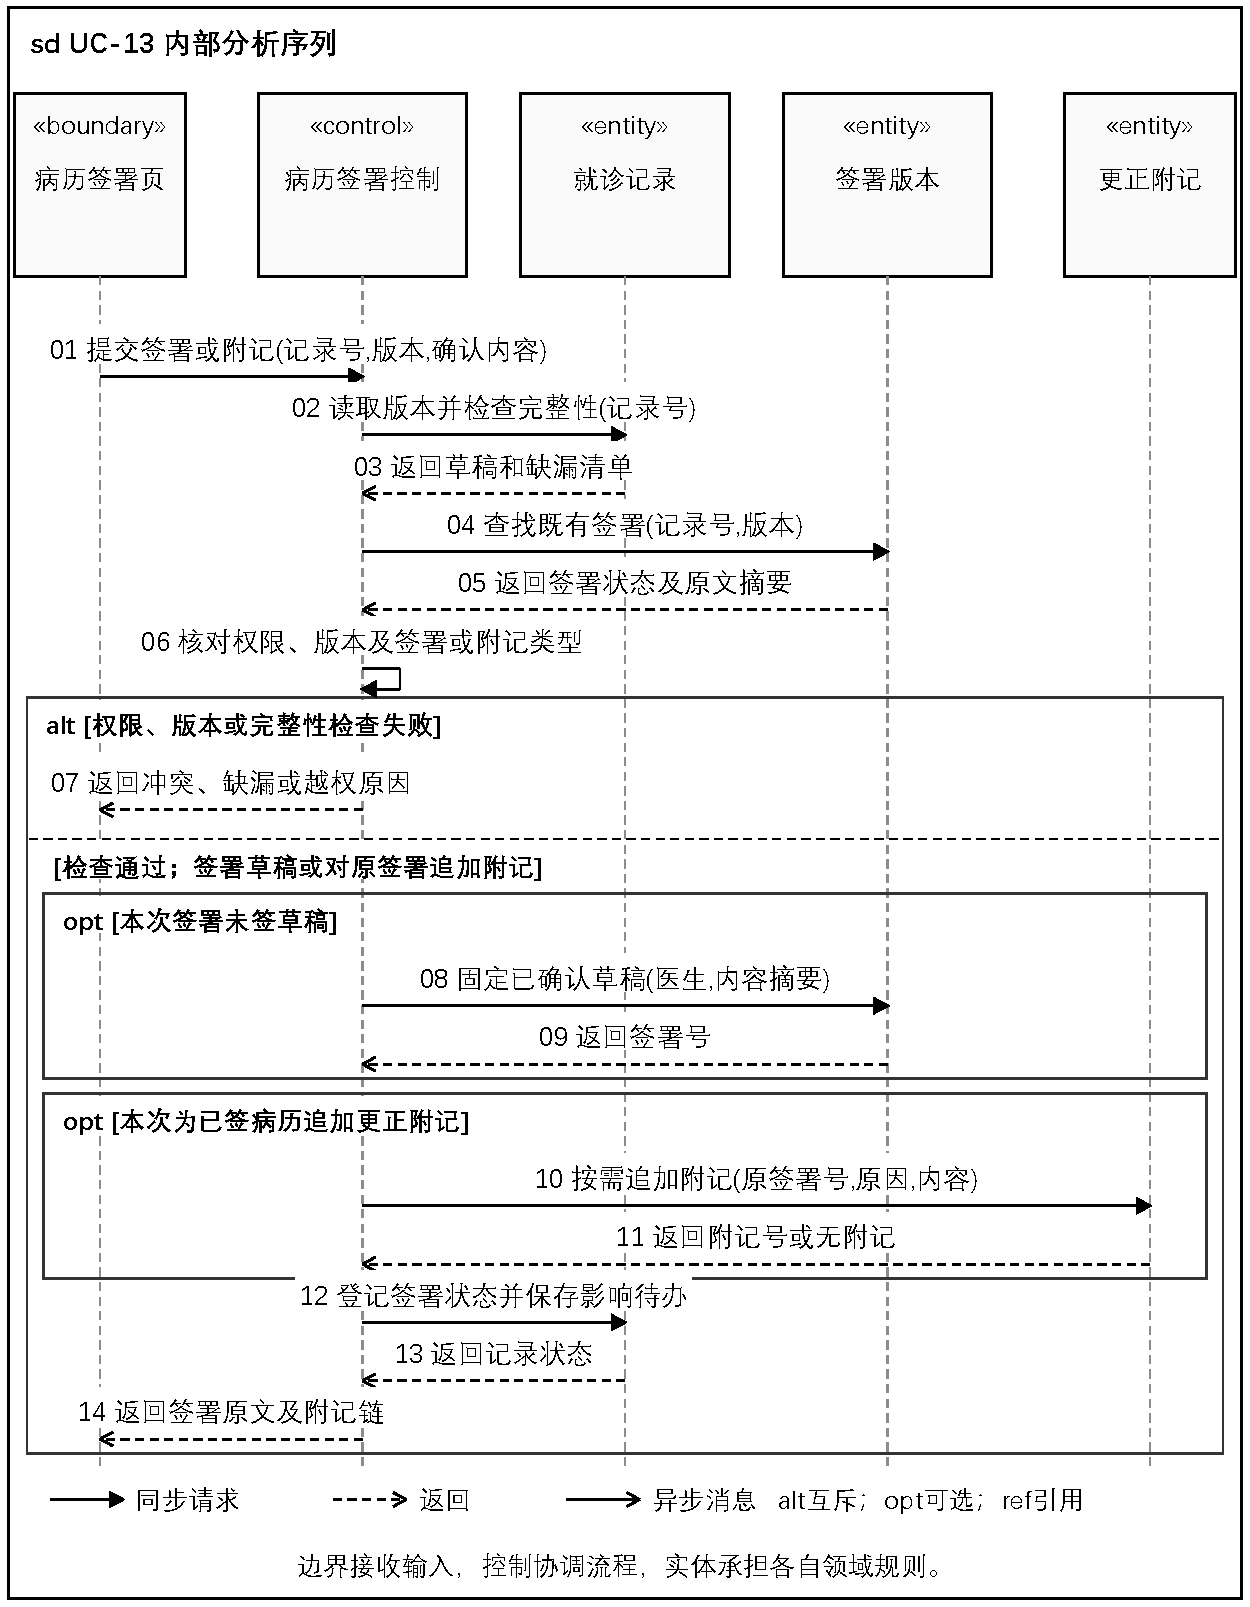
\includegraphics[width=\textwidth]{figures/seq_UC_13.pdf}
\caption{UC-13 内部分析序列}\label{seq_UC_13}\end{figure}
\par\noindent\begin{minipage}{\textwidth}
{\fontsize{10.5pt}{13.2pt}\selectfont\setlength{\tabcolsep}{0pt}\renewcommand{\arraystretch}{1.08}
\captionof{table}{UC-13操作契约 1}\label{tab296}
\begin{tabular}{@{}p{2.640cm}@{\hspace{0.16cm}}p{12.640cm}@{}}
\toprule
\bfseries \Cell{项目} & \bfseries \Cell{详细设计}\\\midrule
\Cell{签名} & \Cell{sign\allowbreak{}Record(\allowbreak{}record\allowbreak{}Id,\allowbreak{} expected\allowbreak{}Version,\allowbreak{} request\allowbreak{}Id)\allowbreak{}:\allowbreak{} Signed\allowbreak{}Record}\\[1pt]
\Cell{输入} & \Cell{记录号、期望版本及医生确认的完整内容}\\[1pt]
\Cell{执行前检查} & \Cell{责任医生已确认；草稿完整且版本一致}\\[1pt]
\Cell{成功结果} & \Cell{唯一签署快照建立，草稿锁定}\\[1pt]
\Cell{领域算法} & \Cell{比对草稿与实际执行清单；核查诊断、牙位、医嘱后生成内容摘要，检查同版本是否已签署；无冲突才固定内容并锁定草稿。}\\[1pt]
\Cell{数据访问} & \Cell{就诊记录仓储读取草稿及执行关联；签署版本仓储保存快照和请求号。}\\[1pt]
\Cell{事务与并发} & \Cell{同一事务比较并交换草稿版本、插入签署版本、登记通知待办；任一步失败全部回滚。}\\[1pt]
\Cell{失败及恢复} & \Cell{版本冲突返回当前摘要；请求重试查回原签署；通知发送失败仅重试待办，不重复签署。}\\[1pt]
\bottomrule\end{tabular}
}\end{minipage}\par\vspace{6pt}
\par\noindent\begin{minipage}{\textwidth}
{\fontsize{10.5pt}{13.2pt}\selectfont\setlength{\tabcolsep}{0pt}\renewcommand{\arraystretch}{1.08}
\captionof{table}{UC-13操作契约 2}\label{tab297}
\begin{tabular}{@{}p{2.640cm}@{\hspace{0.16cm}}p{12.640cm}@{}}
\toprule
\bfseries \Cell{项目} & \bfseries \Cell{详细设计}\\\midrule
\Cell{签名} & \Cell{append\allowbreak{}Correction(\allowbreak{}signed\allowbreak{}Id,\allowbreak{} reason,\allowbreak{} content,\allowbreak{} request\allowbreak{}Id)\allowbreak{}:\allowbreak{} Addendum}\\[1pt]
\Cell{输入} & \Cell{原签署号、更正理由、内容及影响项}\\[1pt]
\Cell{执行前检查} & \Cell{原签署存在且医生获授权}\\[1pt]
\Cell{成功结果} & \Cell{原文保留，新增带签署身份的附记}\\[1pt]
\Cell{领域算法} & \Cell{读取原签署并向医生显示对照；禁止空理由和原文替换，识别是否影响后续医嘱或收费，追加附记并创建对应核对任务。}\\[1pt]
\Cell{数据访问} & \Cell{更正附记仓储按原签署追加；待办仓储登记接续医生或费用核对任务。}\\[1pt]
\Cell{事务与并发} & \Cell{附记及影响任务原子保存；以请求号防止重复追加。}\\[1pt]
\Cell{失败及恢复} & \Cell{原文摘要异常则停止保存；失败保留输入；后续核对未办结不抹去已签附记。}\\[1pt]
\bottomrule\end{tabular}
}\end{minipage}\par\vspace{6pt}
\par\noindent\begin{minipage}{\textwidth}
{\fontsize{10.5pt}{13.2pt}\selectfont\setlength{\tabcolsep}{0pt}\renewcommand{\arraystretch}{1.08}
\captionof{table}{UC-13表示与验收}\label{tab298}
\begin{tabular}{@{}p{2.640cm}@{\hspace{0.16cm}}p{12.640cm}@{}}
\toprule
\bfseries \Cell{项目} & \bfseries \Cell{设计}\\\midrule
\Cell{界面} & \Cell{以原文、附记时间线和待办显示更正链；签署前展示完整预览。}\\[1pt]
\Cell{接口} & \Cell{POST /\allowbreak{}visits/\allowbreak{}\{visit\allowbreak{}Id\}/\allowbreak{}record/\allowbreak{}sign；POST /\allowbreak{}signed-\allowbreak{}records/\allowbreak{}\{id\}/\allowbreak{}addenda。}\\[1pt]
\Cell{验收场景} & \Cell{1.\allowbreak{} 两次提交同一版本→只有一个签署号。\\2.\allowbreak{} 签署后更正牙位→原文仍可见，新增附记并产生费用核对任务。\\3.\allowbreak{} 店长代签→拒绝且不改变病历状态。}\\[1pt]
\bottomrule\end{tabular}
}\end{minipage}\par\vspace{6pt}
\Needspace{497pt}
\subsubsection{UC-14 安排复诊及跨店诊疗交接}
边界：复诊交接页；控制：复诊交接控制。\par
\begin{figure}[H]\centering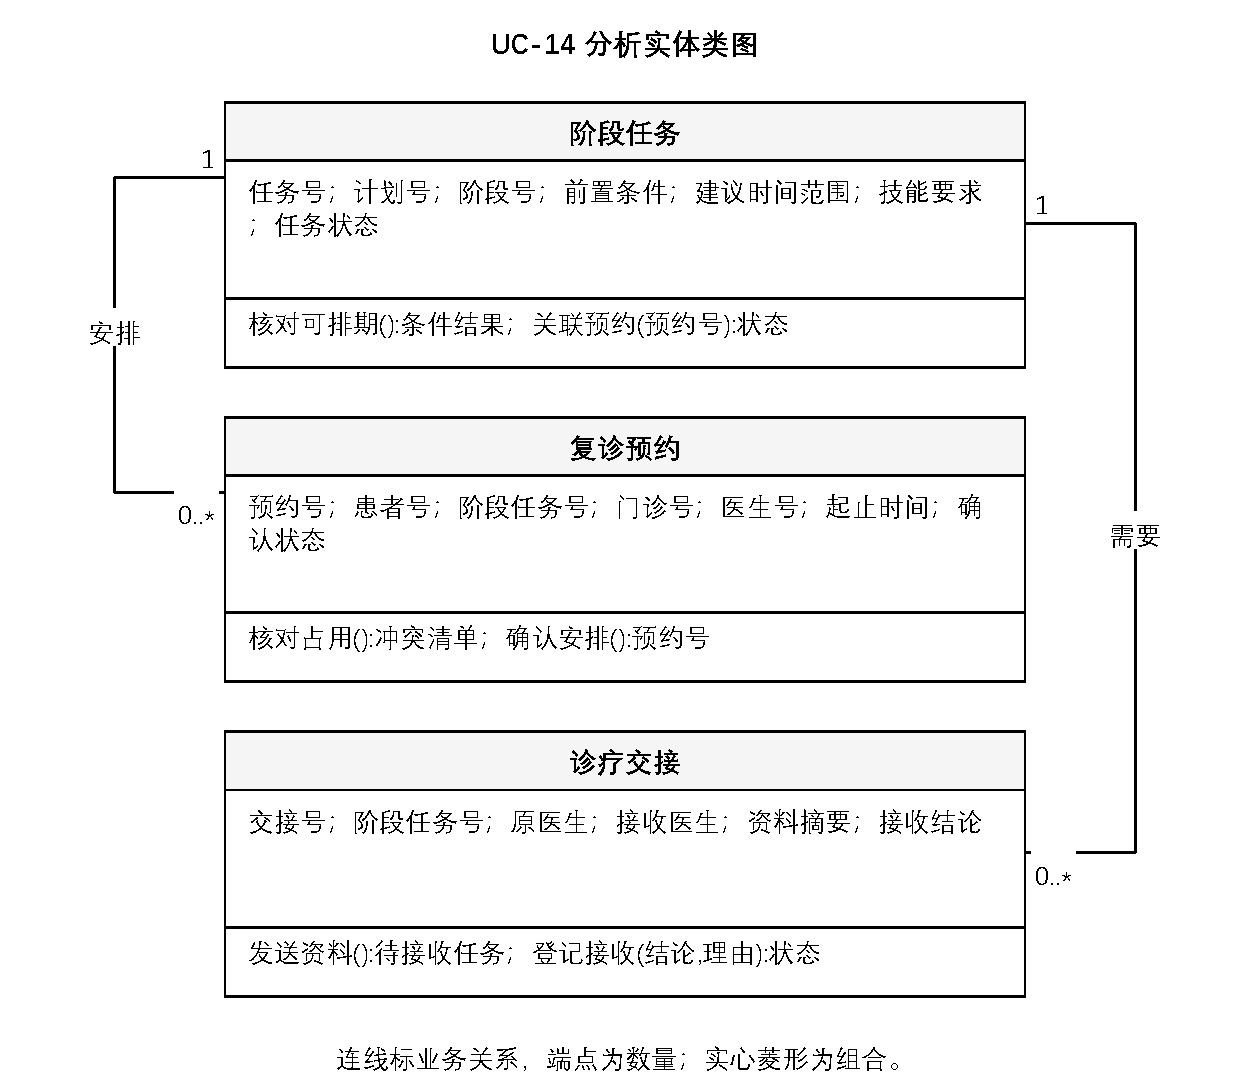
\includegraphics[width=\textwidth]{figures/class_UC_14.pdf}
\caption{UC-14 分析实体类图}\label{class_UC_14}\end{figure}
\begin{figure}[H]\centering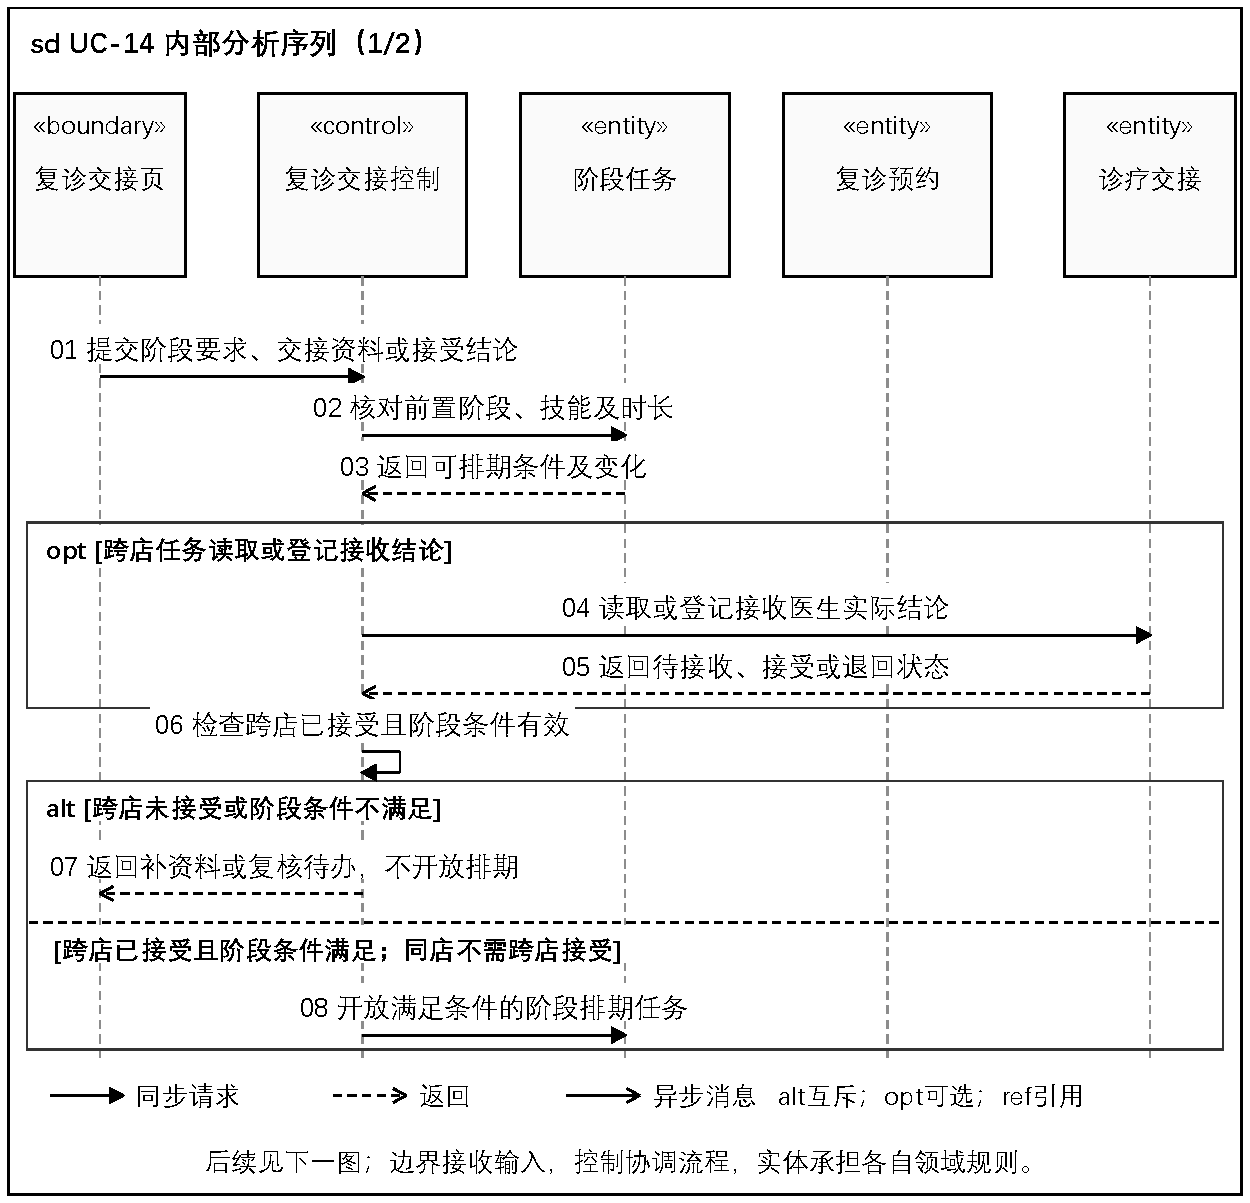
\includegraphics[width=\textwidth]{figures/seq_UC_14_1.pdf}
\caption{UC-14 内部分析序列（1/2）}\label{seq_UC_14_1}\end{figure}
\begin{figure}[H]\centering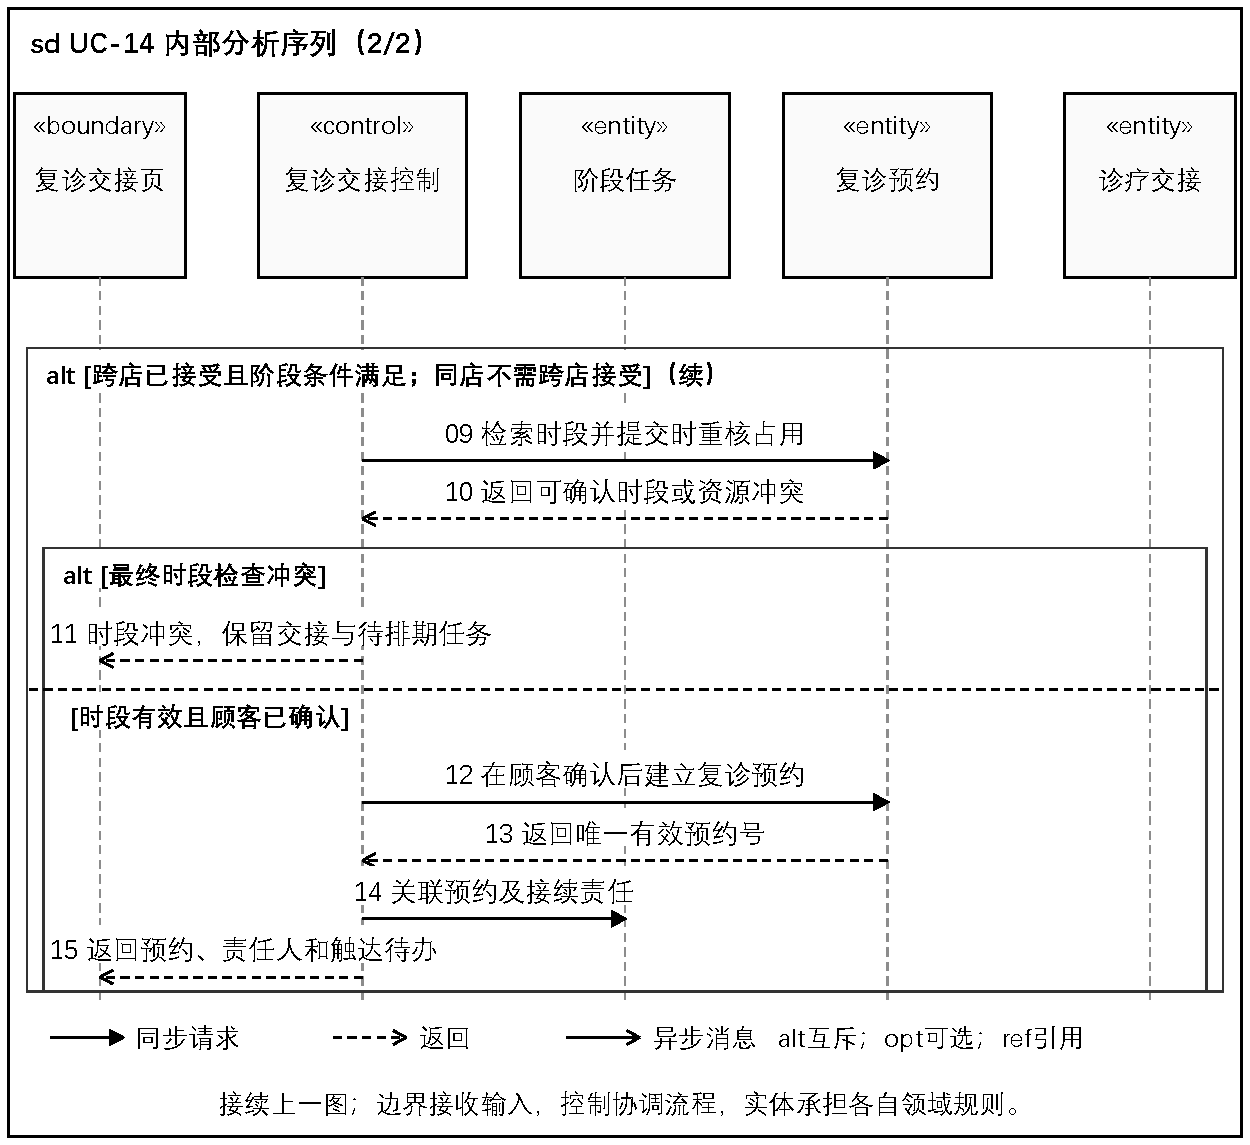
\includegraphics[width=\textwidth]{figures/seq_UC_14_2.pdf}
\caption{UC-14 内部分析序列（2/2）}\label{seq_UC_14_2}\end{figure}
\par\noindent\begin{minipage}{\textwidth}
{\fontsize{10.5pt}{13.2pt}\selectfont\setlength{\tabcolsep}{0pt}\renewcommand{\arraystretch}{1.08}
\captionof{table}{UC-14操作契约 1}\label{tab304}
\begin{tabular}{@{}p{2.640cm}@{\hspace{0.16cm}}p{12.640cm}@{}}
\toprule
\bfseries \Cell{项目} & \bfseries \Cell{详细设计}\\\midrule
\Cell{签名} & \Cell{schedule\allowbreak{}Next\allowbreak{}Stage(\allowbreak{}task\allowbreak{}Id,\allowbreak{} slot\allowbreak{}Id,\allowbreak{} patient\allowbreak{}Confirmation,\allowbreak{} request\allowbreak{}Id)\allowbreak{}:\allowbreak{} Appointment}\\[1pt]
\Cell{输入} & \Cell{阶段任务、候选时段和顾客确认}\\[1pt]
\Cell{执行前检查} & \Cell{阶段可排期，跨店时接收医生已明确接受，顾客已确认安排}\\[1pt]
\Cell{成功结果} & \Cell{一次确认生成一个有效预约}\\[1pt]
\Cell{领域算法} & \Cell{读取阶段条件；跨店时读取接收医生接受结论及其资料版本，条件实质变化先重新接收，未接受不开放正式预约。同店不要求跨店接受；满足相应条件后核对技能、日期、时长和资源冲突，再创建阶段关联预约。}\\[1pt]
\Cell{数据访问} & \Cell{阶段任务仓储读取顺序及条件；预约仓储查询目标门诊资源并保存预约。}\\[1pt]
\Cell{事务与并发} & \Cell{任务版本检查、资源占用和预约创建在同一事务；冲突则均不写入。}\\[1pt]
\Cell{失败及恢复} & \Cell{交接待接收或退回时返回补充任务；号源被占用返回重选；重复请求返回原预约，通知失败重试待办。}\\[1pt]
\bottomrule\end{tabular}
}\end{minipage}\par\vspace{6pt}
\par\noindent\begin{minipage}{\textwidth}
{\fontsize{10.5pt}{13.2pt}\selectfont\setlength{\tabcolsep}{0pt}\renewcommand{\arraystretch}{1.08}
\captionof{table}{UC-14操作契约 2}\label{tab305}
\begin{tabular}{@{}p{2.640cm}@{\hspace{0.16cm}}p{12.640cm}@{}}
\toprule
\bfseries \Cell{项目} & \bfseries \Cell{详细设计}\\\midrule
\Cell{签名} & \Cell{accept\allowbreak{}Handover(\allowbreak{}handover\allowbreak{}Id,\allowbreak{} decision,\allowbreak{} reason,\allowbreak{} expected\allowbreak{}Version)\allowbreak{}:\allowbreak{} Handover}\\[1pt]
\Cell{输入} & \Cell{接收或退回结论及理由}\\[1pt]
\Cell{执行前检查} & \Cell{当前医生是目标接收人，交接待处理}\\[1pt]
\Cell{成功结果} & \Cell{接受后开放满足阶段条件的排期入口；退回后保留原责任与补充待办}\\[1pt]
\Cell{领域算法} & \Cell{核对签署病历及阶段摘要是否齐全；接收医生亲自作出结论，接受则关联接续任务，退回则列明缺项并通知原医生补充。}\\[1pt]
\Cell{数据访问} & \Cell{交接仓储保存结论及资料版本；任务仓储更新责任交接记录。}\\[1pt]
\Cell{事务与并发} & \Cell{交接结论与责任任务原子提交，拒绝覆盖其他人的新结论。}\\[1pt]
\Cell{失败及恢复} & \Cell{资料版本已变化要求重新阅览；接收人停用则退回前台协调，不自动转交任意医生。}\\[1pt]
\bottomrule\end{tabular}
}\end{minipage}\par\vspace{6pt}
\par\noindent\begin{minipage}{\textwidth}
{\fontsize{10.5pt}{13.2pt}\selectfont\setlength{\tabcolsep}{0pt}\renewcommand{\arraystretch}{1.08}
\captionof{table}{UC-14表示与验收}\label{tab306}
\begin{tabular}{@{}p{2.640cm}@{\hspace{0.16cm}}p{12.640cm}@{}}
\toprule
\bfseries \Cell{项目} & \bfseries \Cell{设计}\\\midrule
\Cell{界面} & \Cell{先显示待接收、退回补充、已接受与阶段条件；条件满足后才显示可用排期入口。}\\[1pt]
\Cell{接口} & \Cell{POST /\allowbreak{}stage-\allowbreak{}tasks/\allowbreak{}\{id\}/\allowbreak{}appointments；POST /\allowbreak{}handovers/\allowbreak{}\{id\}/\allowbreak{}decision。}\\[1pt]
\Cell{验收场景} & \Cell{1.\allowbreak{} 跨店交接尚未接受→无法确认该阶段预约。\\2.\allowbreak{} 接收后阶段条件变化→须重新核对，不能沿用旧接受结论。\\3.\allowbreak{} 接收已完成但号源抢占→保留待排期任务，不产生重复预约。}\\[1pt]
\bottomrule\end{tabular}
}\end{minipage}\par\vspace{6pt}
\Needspace{497pt}
\subsubsection{UC-15 生成单次就诊结算单}
边界：就诊结算页；控制：结算单生成控制。\par
\begin{figure}[H]\centering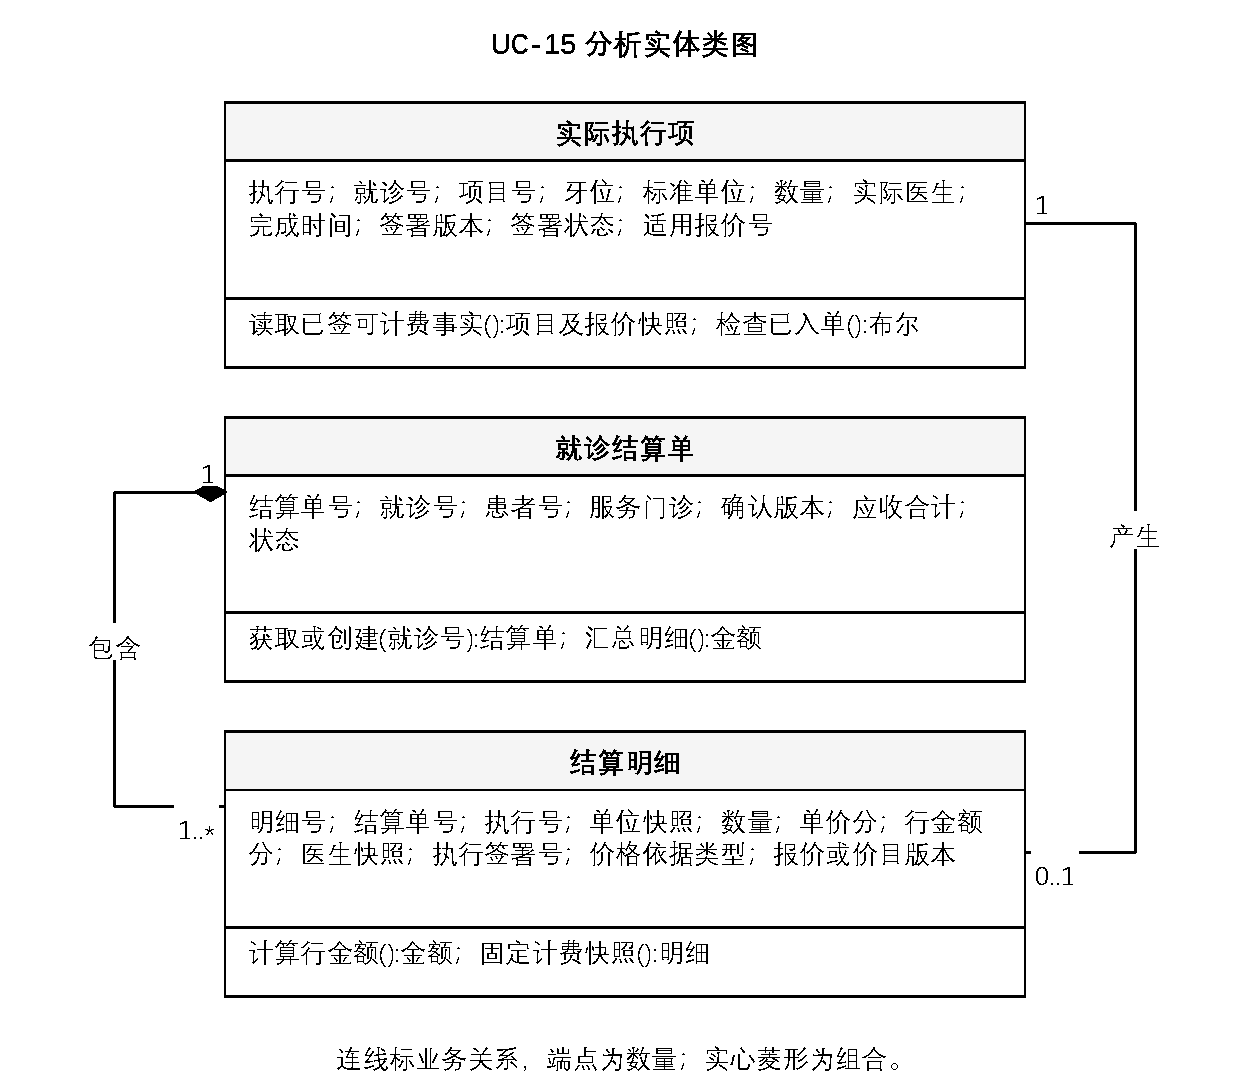
\includegraphics[width=\textwidth]{figures/class_UC_15.pdf}
\caption{UC-15 分析实体类图}\label{class_UC_15}\end{figure}
\begin{figure}[H]\centering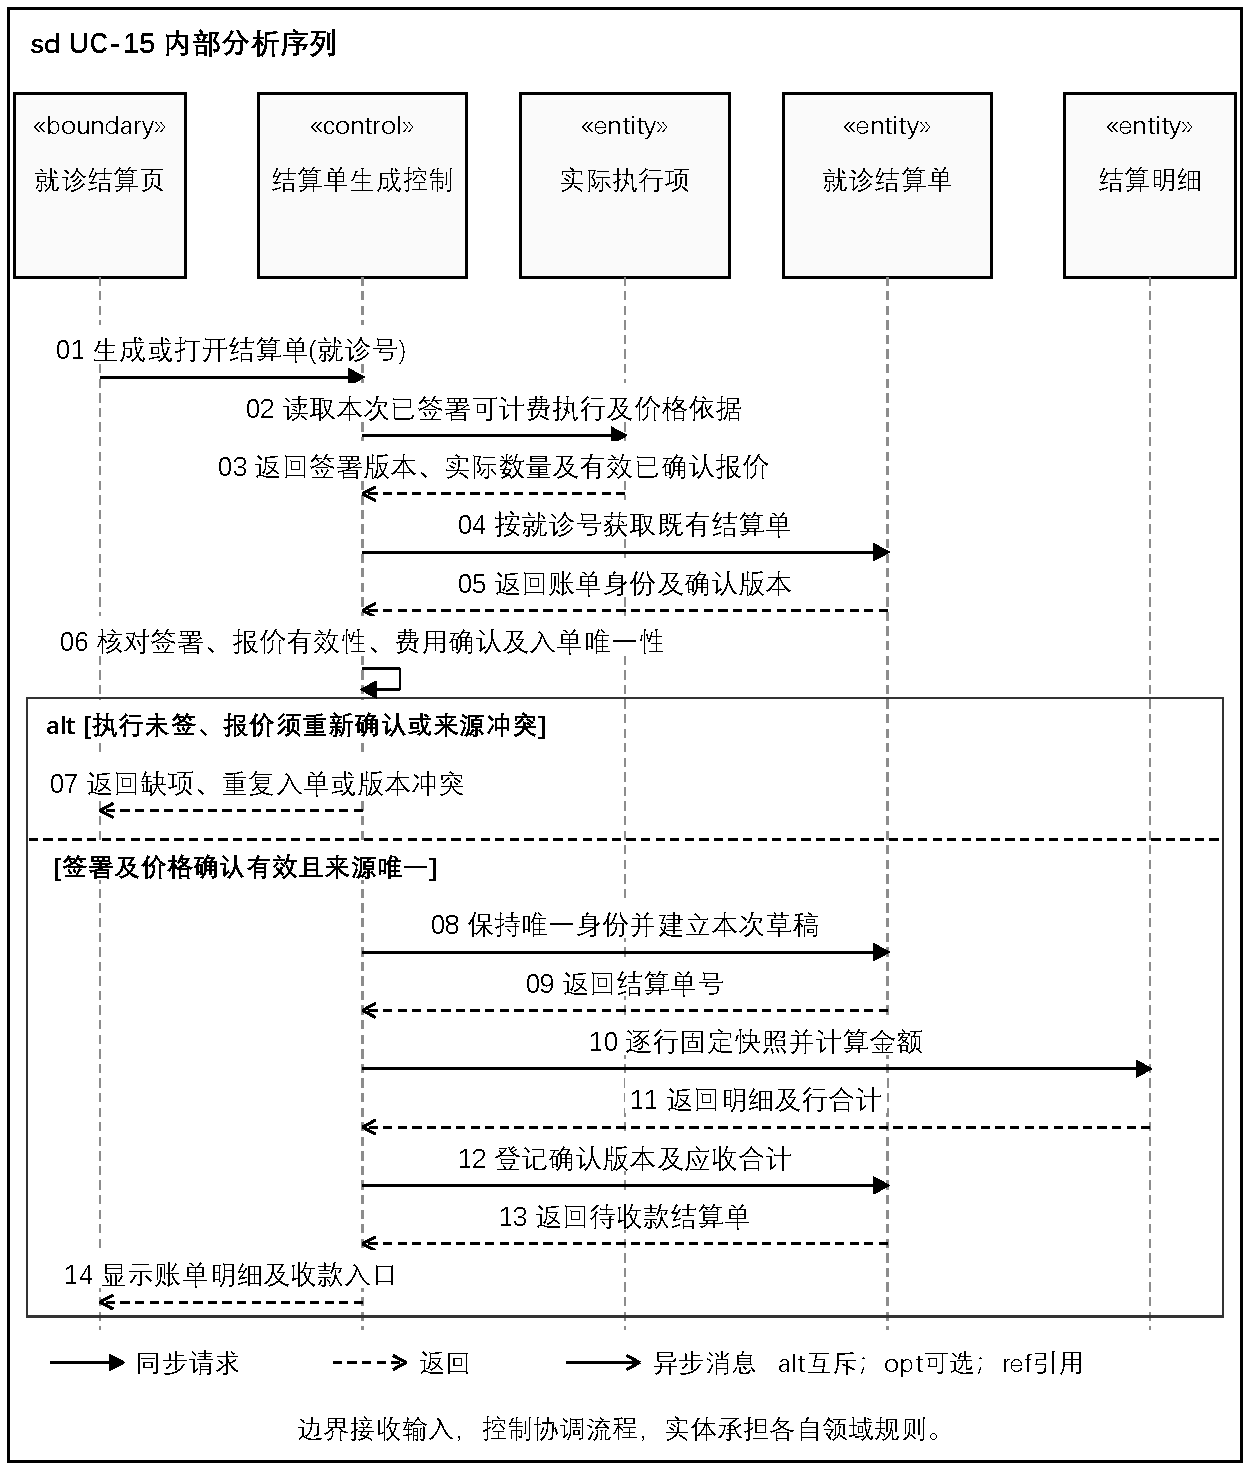
\includegraphics[width=\textwidth]{figures/seq_UC_15.pdf}
\caption{UC-15 内部分析序列}\label{seq_UC_15}\end{figure}
\par\noindent\begin{minipage}{\textwidth}
{\fontsize{10.5pt}{13.2pt}\selectfont\setlength{\tabcolsep}{0pt}\renewcommand{\arraystretch}{1.08}
\captionof{table}{UC-15操作契约}\label{tab311}
\begin{tabular}{@{}p{2.640cm}@{\hspace{0.16cm}}p{12.640cm}@{}}
\toprule
\bfseries \Cell{项目} & \bfseries \Cell{详细设计}\\\midrule
\Cell{签名} & \Cell{prepare\allowbreak{}Visit\allowbreak{}Invoice(\allowbreak{}visit\allowbreak{}Id,\allowbreak{} expected\allowbreak{}Version,\allowbreak{} request\allowbreak{}Id)\allowbreak{}:\allowbreak{} Invoice}\\[1pt]
\Cell{输入} & \Cell{就诊号、执行签署版本和已核对费用依据}\\[1pt]
\Cell{执行前检查} & \Cell{实际执行已签署；有效已确认报价，或无预报价时服务日适用价已说明确认}\\[1pt]
\Cell{成功结果} & \Cell{唯一结算单含可追溯明细}\\[1pt]
\Cell{领域算法} & \Cell{按就诊查原单，读取本次已签且未入单执行；优先采用仍有效的已确认报价，无预报价才取服务日有效价；报价过期或实质变化转重新说明确认；固定签署及价格依据，按实际单位数量四舍五入计算行额并确认唯一账单。}\\[1pt]
\Cell{数据访问} & \Cell{执行项仓储按就诊查询；结算单仓储以就诊唯一键获取或创建；明细仓储以执行号唯一引用保存。}\\[1pt]
\Cell{事务与并发} & \Cell{同一事务锁定账单版本并插入明细、重算合计；唯一键冲突后重新读取原单。}\\[1pt]
\Cell{失败及恢复} & \Cell{未签执行或报价待重新确认返回具体行；并发生成查回原单；已出具明细争议转费用更正，不删除旧明细。}\\[1pt]
\bottomrule\end{tabular}
}\end{minipage}\par\vspace{6pt}
\par\noindent\begin{minipage}{\textwidth}
{\fontsize{10.5pt}{13.2pt}\selectfont\setlength{\tabcolsep}{0pt}\renewcommand{\arraystretch}{1.08}
\captionof{table}{UC-15表示与验收}\label{tab312}
\begin{tabular}{@{}p{2.640cm}@{\hspace{0.16cm}}p{12.640cm}@{}}
\toprule
\bfseries \Cell{项目} & \bfseries \Cell{设计}\\\midrule
\Cell{界面} & \Cell{一页显示实际项目、单位、数量、单价、治疗医生、已收与未收；明确区分方案估价。}\\[1pt]
\Cell{接口} & \Cell{POST /\allowbreak{}visits/\allowbreak{}\{visit\allowbreak{}Id\}/\allowbreak{}invoice/\allowbreak{}prepare；GET /\allowbreak{}visits/\allowbreak{}\{visit\allowbreak{}Id\}/\allowbreak{}invoice。}\\[1pt]
\Cell{验收场景} & \Cell{1.\allowbreak{} 并发生成同一就诊账单→同一单号且项目仅计一次。\\2.\allowbreak{} 历史价格更新→已确认明细单价保持。\\3.\allowbreak{} 收取预收款→不多出本次就诊结算单。\\4.\allowbreak{} 未签署执行→不得出具对应结算明细。\\5.\allowbreak{} 有效报价后目录涨价→仍采用已确认报价；过期报价→重新确认后才能出单。\\6.\allowbreak{} 账单500元仅收300元→收入依据500元，应收余额200元。}\\[1pt]
\bottomrule\end{tabular}
}\end{minipage}\par\vspace{6pt}
\Needspace{608pt}
\subsubsection{UC-16 确认收款并分配到应收}
边界：收款核销页；控制：收款确认控制。\par
\begin{figure}[H]\centering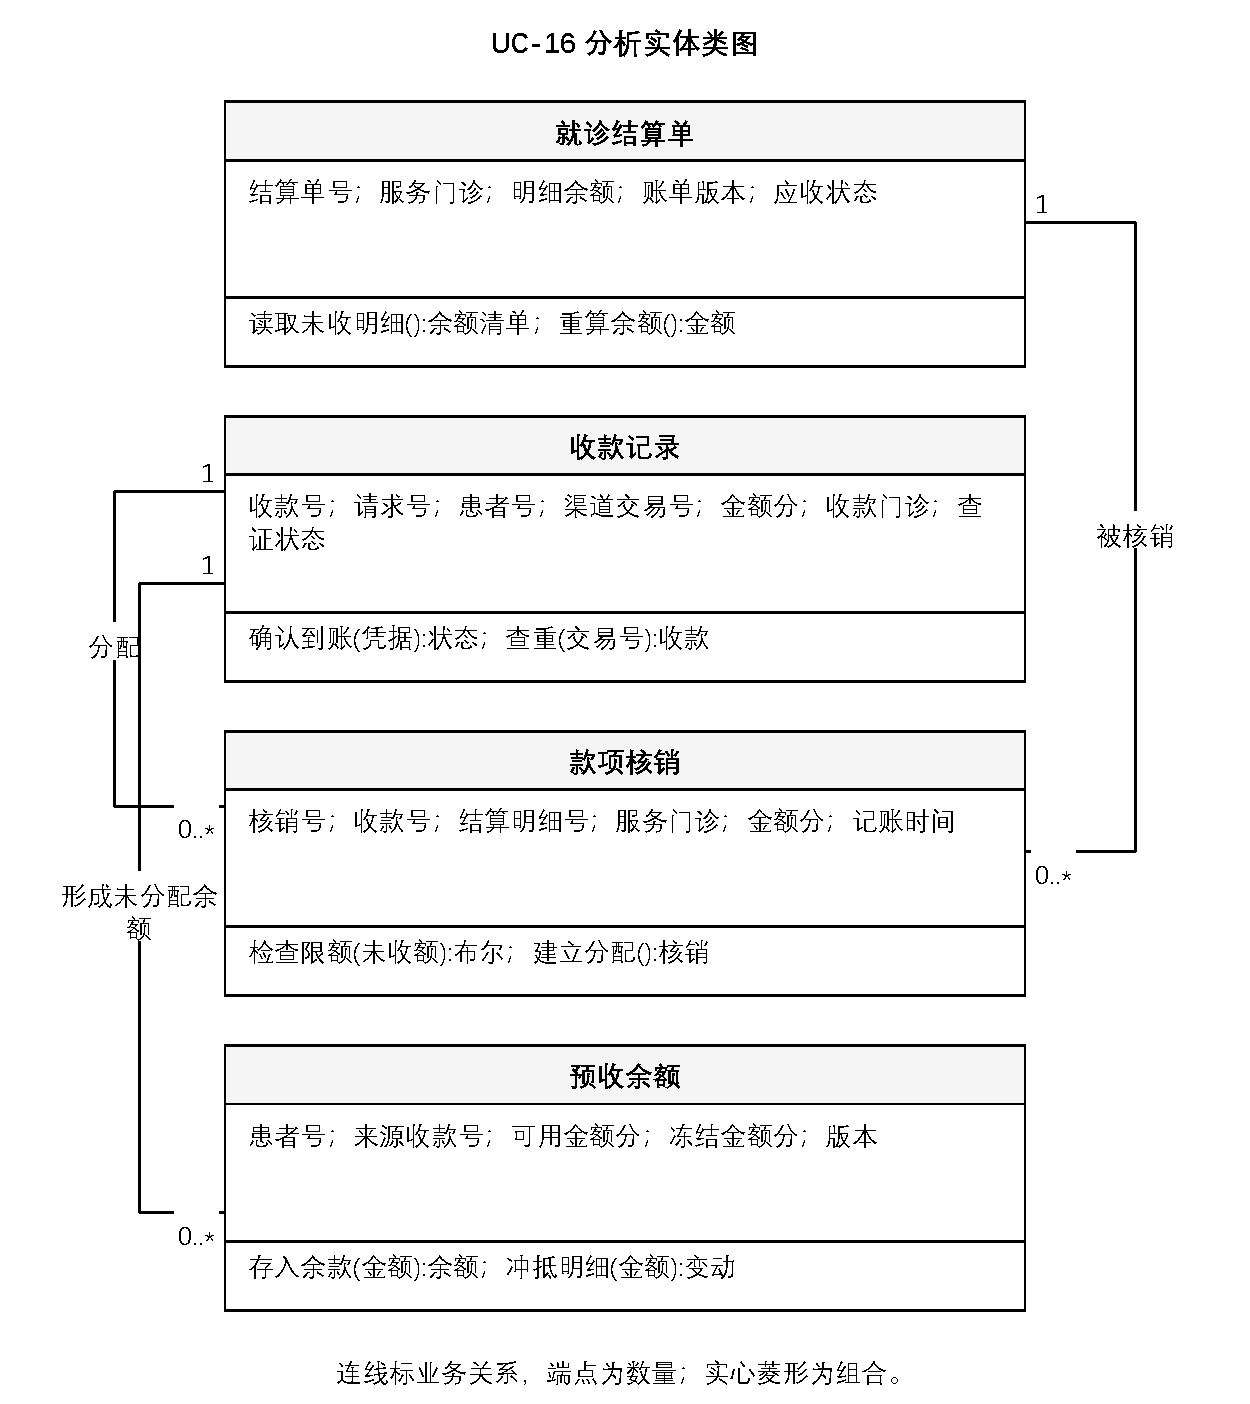
\includegraphics[width=\textwidth]{figures/class_UC_16.pdf}
\caption{UC-16 分析实体类图}\label{class_UC_16}\end{figure}
\begin{figure}[H]\centering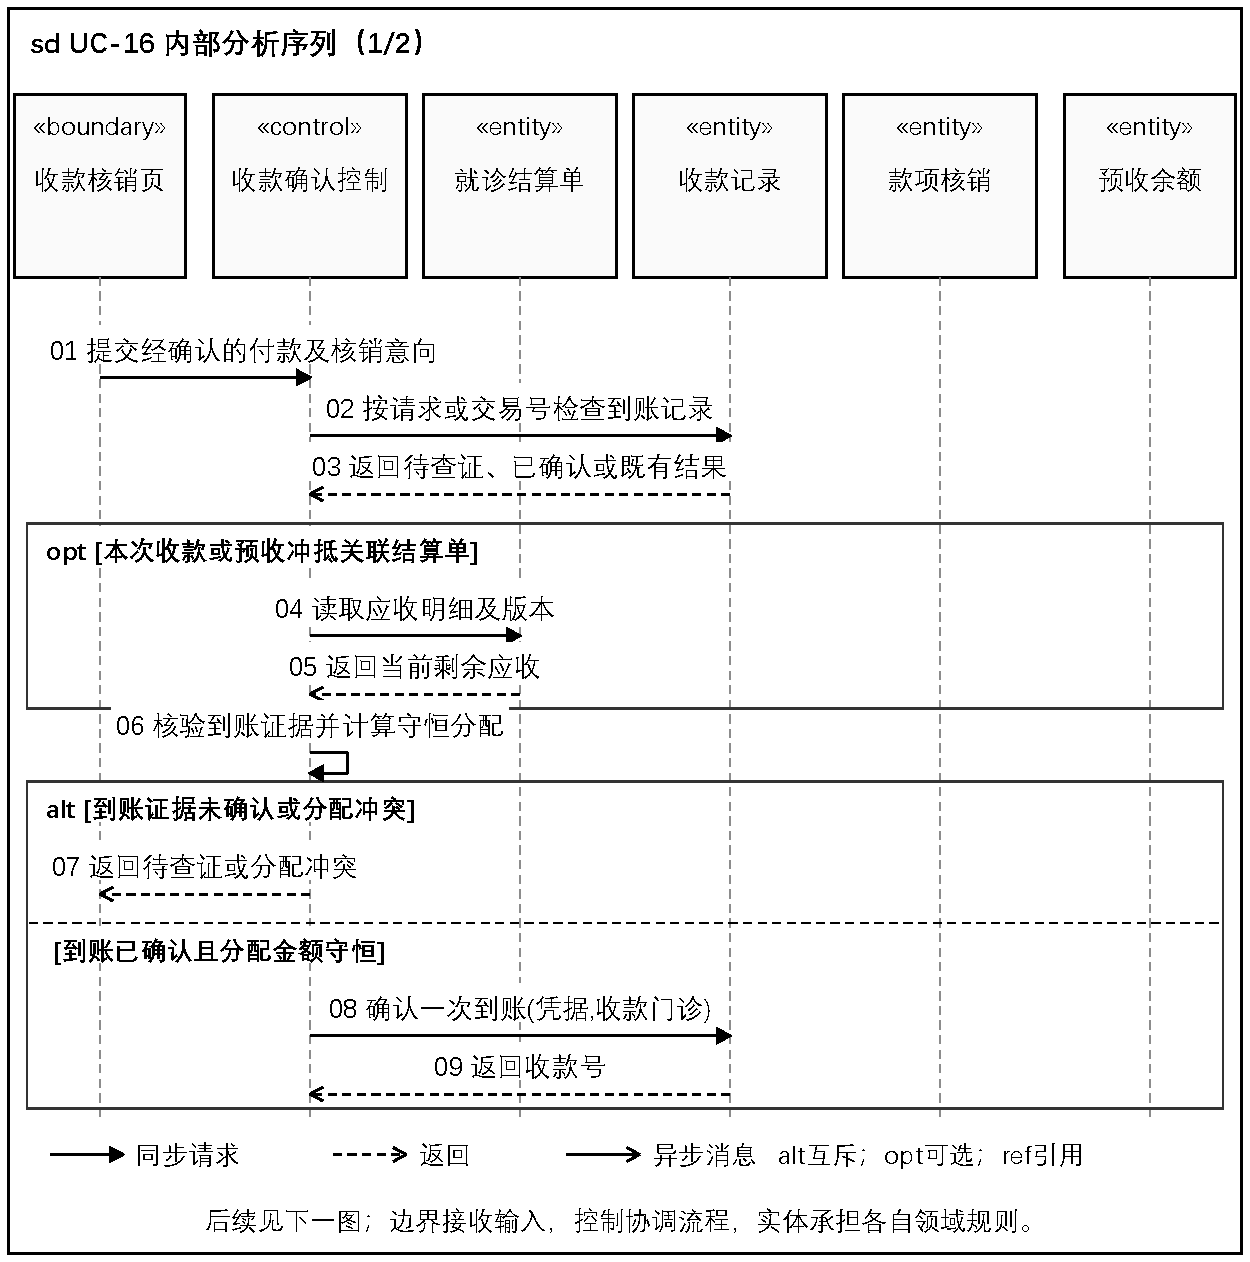
\includegraphics[width=\textwidth]{figures/seq_UC_16_1.pdf}
\caption{UC-16 内部分析序列（1/2）}\label{seq_UC_16_1}\end{figure}
\begin{figure}[H]\centering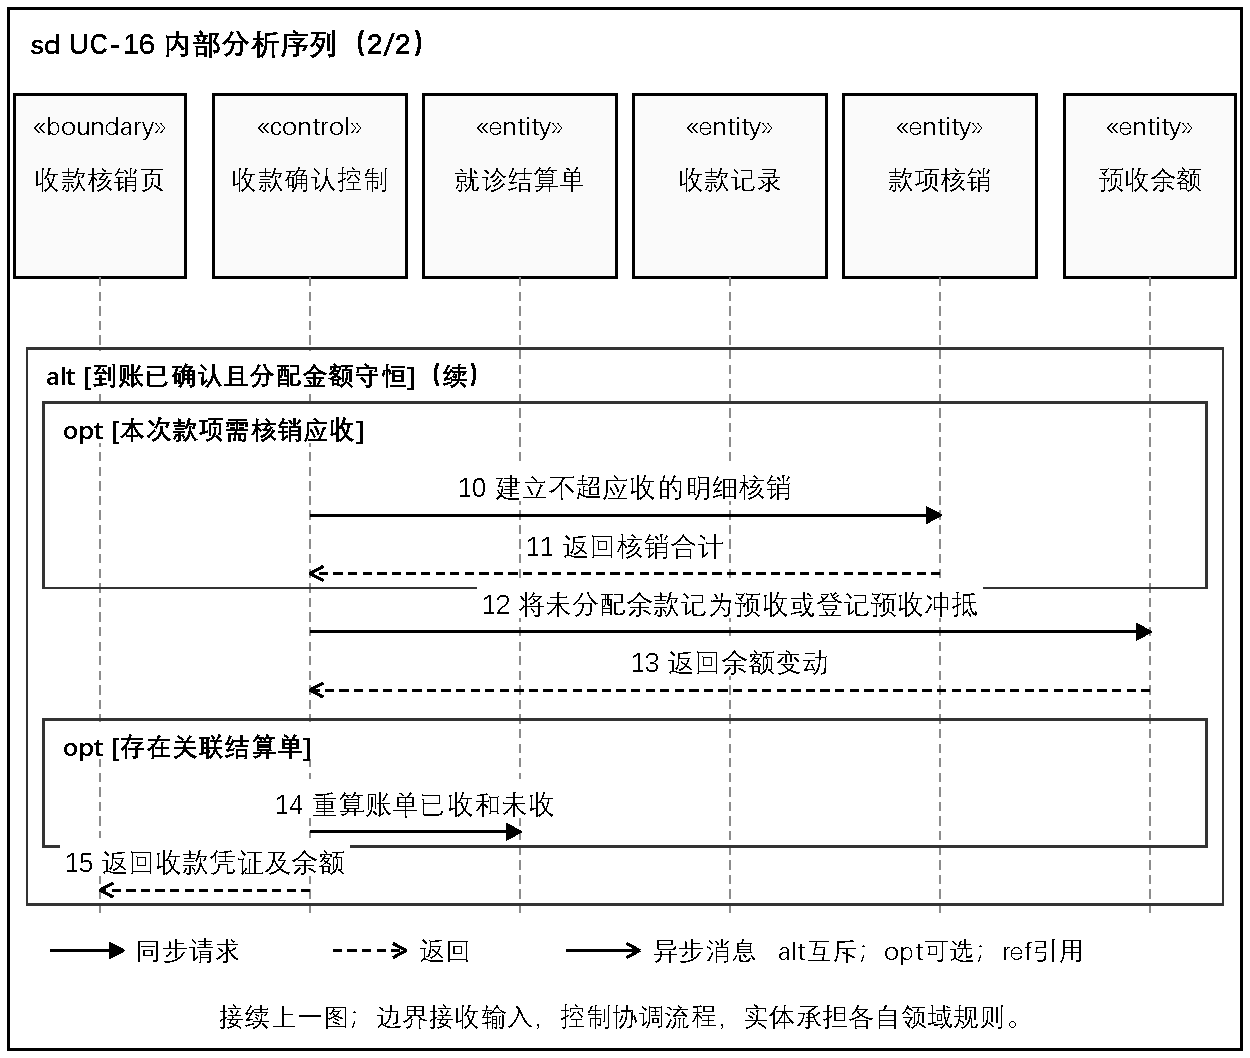
\includegraphics[width=\textwidth]{figures/seq_UC_16_2.pdf}
\caption{UC-16 内部分析序列（2/2）}\label{seq_UC_16_2}\end{figure}
\par\noindent\begin{minipage}{\textwidth}
{\fontsize{10.5pt}{13.2pt}\selectfont\setlength{\tabcolsep}{0pt}\renewcommand{\arraystretch}{1.08}
\captionof{table}{UC-16操作契约 1}\label{tab318}
\begin{tabular}{@{}p{2.640cm}@{\hspace{0.16cm}}p{12.640cm}@{}}
\toprule
\bfseries \Cell{项目} & \bfseries \Cell{详细设计}\\\midrule
\Cell{签名} & \Cell{confirm\allowbreak{}Receipt(\allowbreak{}request\allowbreak{}Id,\allowbreak{} evidence,\allowbreak{} clinic\allowbreak{}Id)\allowbreak{}:\allowbreak{} Receipt}\\[1pt]
\Cell{输入} & \Cell{请求号、有效到账证据及收款门诊}\\[1pt]
\Cell{执行前检查} & \Cell{现金点收或渠道结果已独立核实}\\[1pt]
\Cell{成功结果} & \Cell{到账只登记一次}\\[1pt]
\Cell{领域算法} & \Cell{校验渠道来源、交易号、金额和请求；查询是否已确认；已确认返回原记录，未确认则固定查证人或回执摘要及收款门诊。}\\[1pt]
\Cell{数据访问} & \Cell{收款仓储按请求及渠道交易唯一键查重；到账证据仓储保存必要凭据摘要。}\\[1pt]
\Cell{事务与并发} & \Cell{确认状态与凭据原子保存；待查证请求保持不记实收；外部查询在事务外完成。}\\[1pt]
\Cell{失败及恢复} & \Cell{回执不匹配进入差异待办；网络不明查询原交易；不以重复发起收款恢复。}\\[1pt]
\bottomrule\end{tabular}
}\end{minipage}\par\vspace{6pt}
\par\noindent\begin{minipage}{\textwidth}
{\fontsize{10.5pt}{13.2pt}\selectfont\setlength{\tabcolsep}{0pt}\renewcommand{\arraystretch}{1.08}
\captionof{table}{UC-16操作契约 2}\label{tab319}
\begin{tabular}{@{}p{2.640cm}@{\hspace{0.16cm}}p{12.640cm}@{}}
\toprule
\bfseries \Cell{项目} & \bfseries \Cell{详细设计}\\\midrule
\Cell{签名} & \Cell{allocate\allowbreak{}Receipt(\allowbreak{}receipt\allowbreak{}Id,\allowbreak{} lines,\allowbreak{} expected\allowbreak{}Versions)\allowbreak{}:\allowbreak{} Allocation\allowbreak{}Result}\\[1pt]
\Cell{输入} & \Cell{收款或可用预收来源、项目与分配额}\\[1pt]
\Cell{执行前检查} & \Cell{款项确认且可用，各明细未收足够}\\[1pt]
\Cell{成功结果} & \Cell{款项去向与应收余额一致}\\[1pt]
\Cell{领域算法} & \Cell{按稳定顺序锁定来源余额及账单，逐项计算剩余应收；分配总额不得超可用额，余款计入预收；预收冲抵只登记余额转移。}\\[1pt]
\Cell{数据访问} & \Cell{核销仓储保存款项—项目联系；预收仓储保存变动；结算仓储重算余额。}\\[1pt]
\Cell{事务与并发} & \Cell{全部核销、预收及应收重算在同一事务；账单版本变化整体回滚重算。}\\[1pt]
\Cell{失败及恢复} & \Cell{额度不足返回冲突行；重复请求返回原分配；失败不留下单边余额变动。}\\[1pt]
\bottomrule\end{tabular}
}\end{minipage}\par\vspace{6pt}
\par\noindent\begin{minipage}{\textwidth}
{\fontsize{10.5pt}{13.2pt}\selectfont\setlength{\tabcolsep}{0pt}\renewcommand{\arraystretch}{1.08}
\captionof{table}{UC-16表示与验收}\label{tab320}
\begin{tabular}{@{}p{2.640cm}@{\hspace{0.16cm}}p{12.640cm}@{}}
\toprule
\bfseries \Cell{项目} & \bfseries \Cell{设计}\\\midrule
\Cell{界面} & \Cell{区分待确认到账、已到账未分配、部分支付与已结清；预收单独展示。}\\[1pt]
\Cell{接口} & \Cell{POST /\allowbreak{}receipts；POST /\allowbreak{}receipts/\allowbreak{}\{id\}/\allowbreak{}confirm；POST /\allowbreak{}receipts/\allowbreak{}\{id\}/\allowbreak{}allocations。}\\[1pt]
\Cell{验收场景} & \Cell{1.\allowbreak{} 同一支付回执推送三次→一笔收款。\\2.\allowbreak{} 支付超过应收→超额列为预收，账单不出现负欠款。\\3.\allowbreak{} 预收抵扣账单→现金流入不增加。}\\[1pt]
\bottomrule\end{tabular}
}\end{minipage}\par\vspace{6pt}
\Needspace{608pt}
\subsubsection{UC-17 审批费用更正并办理退款}
边界：费用更正退款页；控制：费用更正退款控制。\par
\begin{figure}[H]\centering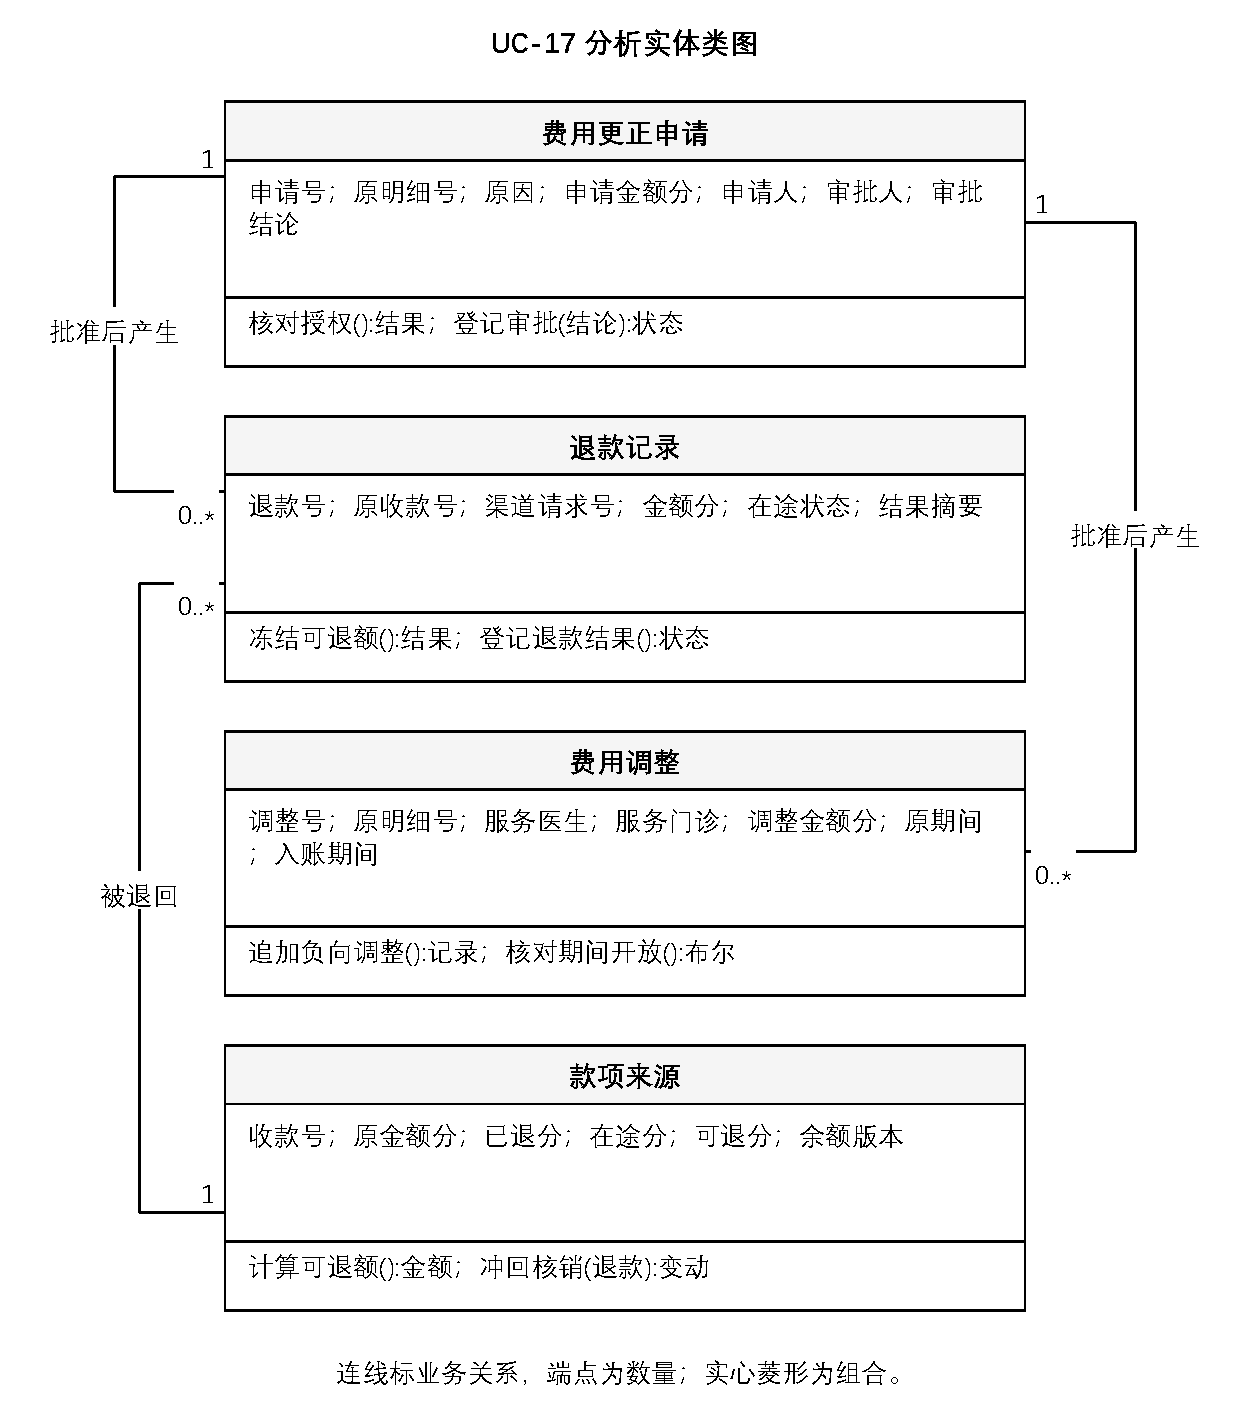
\includegraphics[width=\textwidth]{figures/class_UC_17.pdf}
\caption{UC-17 分析实体类图}\label{class_UC_17}\end{figure}
\begin{figure}[H]\centering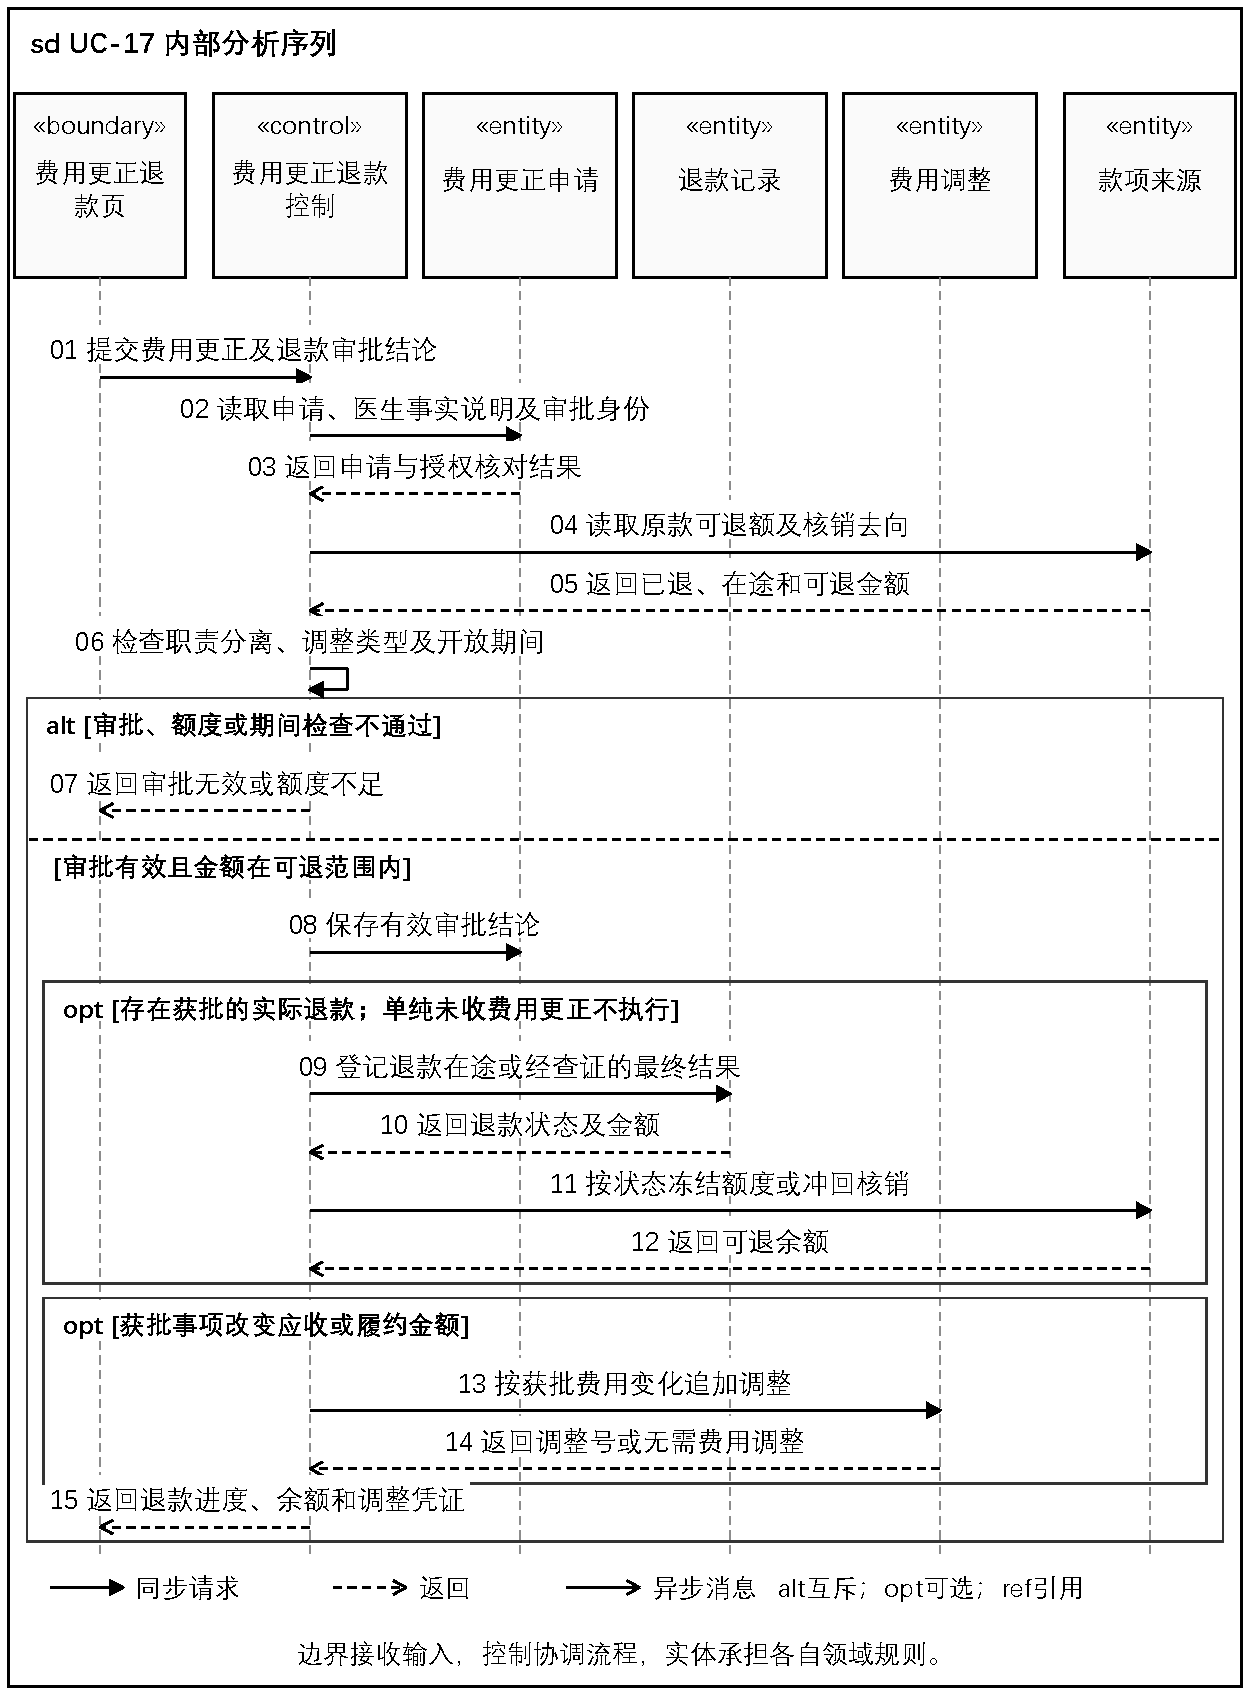
\includegraphics[width=\textwidth]{figures/seq_UC_17.pdf}
\caption{UC-17 内部分析序列}\label{seq_UC_17}\end{figure}
\par\noindent\begin{minipage}{\textwidth}
{\fontsize{10.5pt}{13.2pt}\selectfont\setlength{\tabcolsep}{0pt}\renewcommand{\arraystretch}{1.08}
\captionof{table}{UC-17操作契约 1}\label{tab325}
\begin{tabular}{@{}p{2.640cm}@{\hspace{0.16cm}}p{12.640cm}@{}}
\toprule
\bfseries \Cell{项目} & \bfseries \Cell{详细设计}\\\midrule
\Cell{签名} & \Cell{approve\allowbreak{}Correction(\allowbreak{}application\allowbreak{}Id,\allowbreak{} decision,\allowbreak{} expected\allowbreak{}Version)\allowbreak{}:\allowbreak{} Approval}\\[1pt]
\Cell{输入} & \Cell{审批意见、事实说明与授权身份}\\[1pt]
\Cell{执行前检查} & \Cell{审批人与申请人不同，资料齐全}\\[1pt]
\Cell{成功结果} & \Cell{审批及费用调整依据固定}\\[1pt]
\Cell{领域算法} & \Cell{按调整类型检查是否影响应收、服务收入或仅退多付款；核验医生说明、权限额度和期间，审批通过后锁定原款剩余额度或登记无资金更正。}\\[1pt]
\Cell{数据访问} & \Cell{申请仓储保存审批快照；款项仓储保存退款额度占用；调整仓储引用原项目。}\\[1pt]
\Cell{事务与并发} & \Cell{审批、额度占用与待发退款任务原子写入，费用调整以独立凭证保存，防止重复审批产生双份凭证。}\\[1pt]
\Cell{失败及恢复} & \Cell{超额或自批拒绝；版本变化重读；无实际收款仅生成费用调整不发起退款。}\\[1pt]
\bottomrule\end{tabular}
}\end{minipage}\par\vspace{6pt}
\par\noindent\begin{minipage}{\textwidth}
{\fontsize{10.5pt}{13.2pt}\selectfont\setlength{\tabcolsep}{0pt}\renewcommand{\arraystretch}{1.08}
\captionof{table}{UC-17操作契约 2}\label{tab326}
\begin{tabular}{@{}p{2.640cm}@{\hspace{0.16cm}}p{12.640cm}@{}}
\toprule
\bfseries \Cell{项目} & \bfseries \Cell{详细设计}\\\midrule
\Cell{签名} & \Cell{record\allowbreak{}Refund\allowbreak{}Result(\allowbreak{}refund\allowbreak{}Id,\allowbreak{} verified\allowbreak{}Result)\allowbreak{}:\allowbreak{} Refund}\\[1pt]
\Cell{输入} & \Cell{原退款请求的已核实渠道结果}\\[1pt]
\Cell{执行前检查} & \Cell{退款处于在途或待查证}\\[1pt]
\Cell{成功结果} & \Cell{成功冲回一次，失败释放占用，未知保持在途}\\[1pt]
\Cell{领域算法} & \Cell{核对渠道请求号与金额；最终成功追加退款流水并按原核销路径冲回；最终失败释放冻结；不明结果只记录查证任务。}\\[1pt]
\Cell{数据访问} & \Cell{退款仓储保存结果摘要；核销与预收仓储追加反向变动；流水仓储记录实际退款。}\\[1pt]
\Cell{事务与并发} & \Cell{退款状态、反向核销及额度更新同一事务；渠道发起和查询在事务外执行。}\\[1pt]
\Cell{失败及恢复} & \Cell{重复成功回执返回原结果；相互矛盾回执停止自动记账并交人工核验，不覆盖成功凭证。}\\[1pt]
\bottomrule\end{tabular}
}\end{minipage}\par\vspace{6pt}
\par\noindent\begin{minipage}{\textwidth}
{\fontsize{10.5pt}{13.2pt}\selectfont\setlength{\tabcolsep}{0pt}\renewcommand{\arraystretch}{1.08}
\captionof{table}{UC-17表示与验收}\label{tab327}
\begin{tabular}{@{}p{2.640cm}@{\hspace{0.16cm}}p{12.640cm}@{}}
\toprule
\bfseries \Cell{项目} & \bfseries \Cell{设计}\\\midrule
\Cell{界面} & \Cell{并列显示原账、申请、更正凭证及退款进度，状态不明醒目标注待查证。}\\[1pt]
\Cell{接口} & \Cell{POST /\allowbreak{}corrections；POST /\allowbreak{}corrections/\allowbreak{}\{id\}/\allowbreak{}approval；POST /\allowbreak{}refunds/\allowbreak{}\{id\}/\allowbreak{}verified-\allowbreak{}result。}\\[1pt]
\Cell{验收场景} & \Cell{1.\allowbreak{} 多收款退回→现金净额减少，服务收入不变。\\2.\allowbreak{} 已关账费用纠错→开放期间产生引用原记录的调整。\\3.\allowbreak{} 两笔并发申请超过可退额→至少一笔被拒绝或限额。}\\[1pt]
\bottomrule\end{tabular}
}\end{minipage}\par\vspace{6pt}
\Needspace{497pt}
\subsubsection{UC-18 完成门诊日结及跨店代收核对}
边界：门诊日结页；控制：日结代收核对控制。\par
\begin{figure}[H]\centering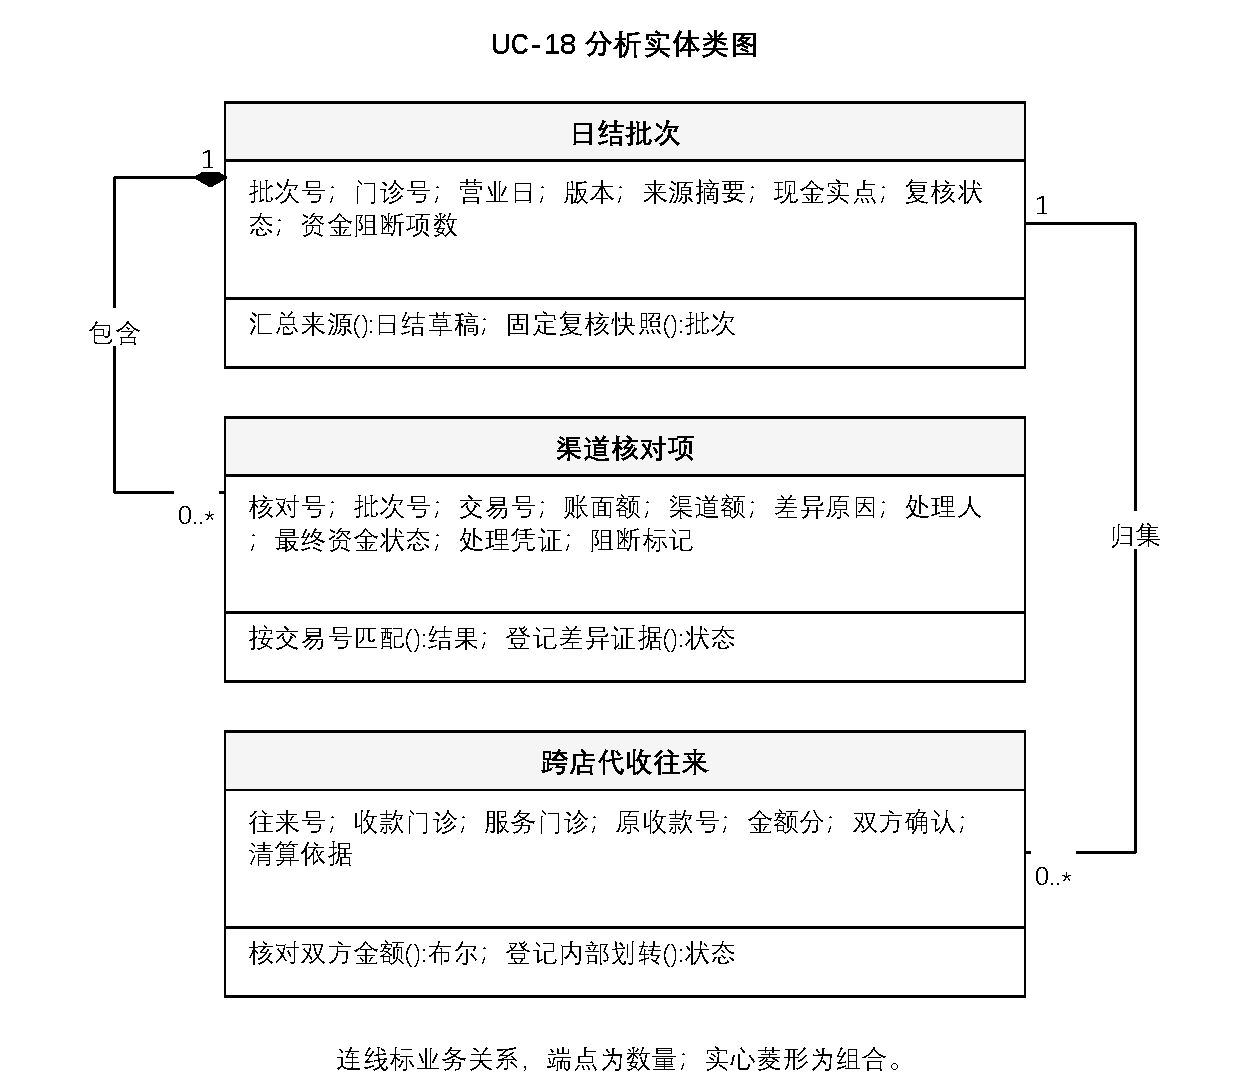
\includegraphics[width=\textwidth]{figures/class_UC_18.pdf}
\caption{UC-18 分析实体类图}\label{class_UC_18}\end{figure}
\begin{figure}[H]\centering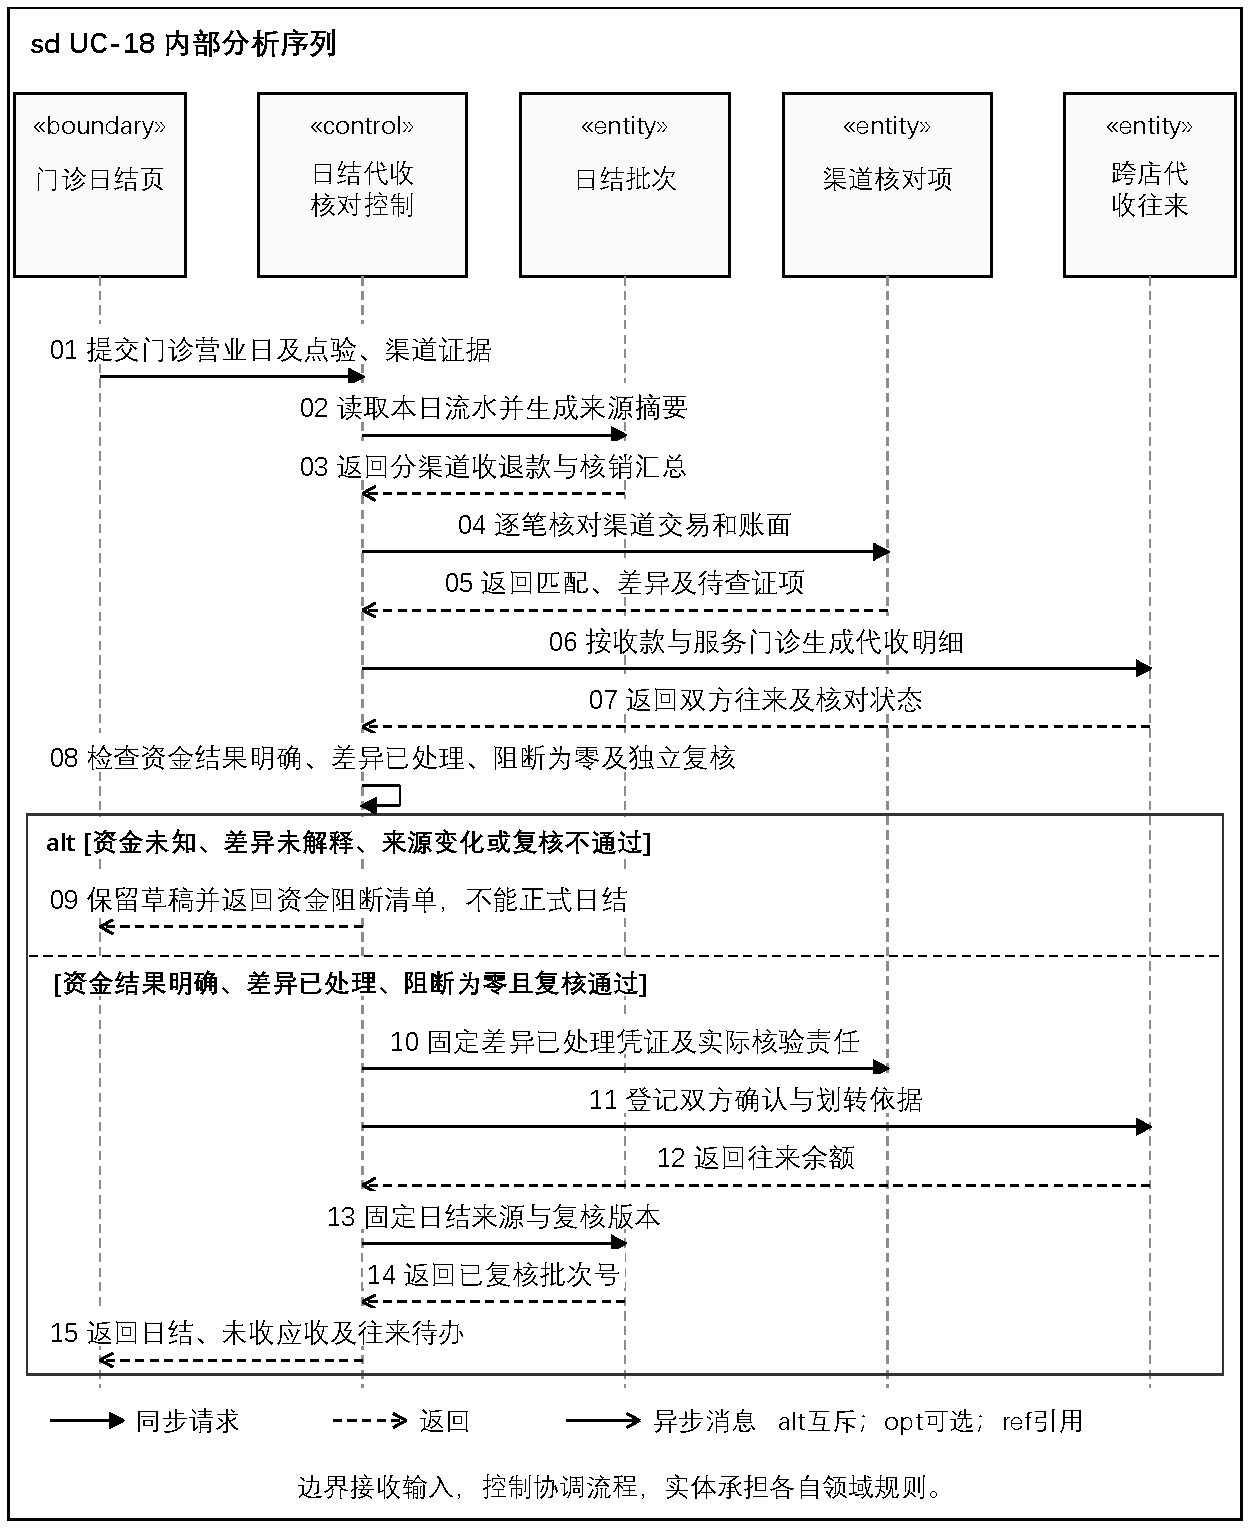
\includegraphics[width=\textwidth]{figures/seq_UC_18.pdf}
\caption{UC-18 内部分析序列}\label{seq_UC_18}\end{figure}
\par\noindent\begin{minipage}{\textwidth}
{\fontsize{10.5pt}{13.2pt}\selectfont\setlength{\tabcolsep}{0pt}\renewcommand{\arraystretch}{1.08}
\captionof{table}{UC-18操作契约 1}\label{tab332}
\begin{tabular}{@{}p{2.640cm}@{\hspace{0.16cm}}p{12.640cm}@{}}
\toprule
\bfseries \Cell{项目} & \bfseries \Cell{详细设计}\\\midrule
\Cell{签名} & \Cell{prepare\allowbreak{}Daily\allowbreak{}Close(\allowbreak{}clinic\allowbreak{}Id,\allowbreak{} business\allowbreak{}Date)\allowbreak{}:\allowbreak{} Close\allowbreak{}Draft}\\[1pt]
\Cell{输入} & \Cell{门诊、营业日、现金实点和渠道账单}\\[1pt]
\Cell{执行前检查} & \Cell{范围权限有效，核验来源可追溯}\\[1pt]
\Cell{成功结果} & \Cell{草稿列明全部匹配及差异}\\[1pt]
\Cell{领域算法} & \Cell{分别按到账日汇总收退款、按核销日汇总项目核销；按渠道交易号匹配收退款，金额不符单列；扫描本日核销中收款门诊不同于服务门诊的分配，含以前预收本日冲抵，按原收款和核销号生成成对往来。}\\[1pt]
\Cell{数据访问} & \Cell{流水仓储按门诊营业日读取；核对项仓储保存匹配证据；往来仓储以原收款和分配唯一键去重。}\\[1pt]
\Cell{事务与并发} & \Cell{生成带来源摘要的草稿版本；重算不覆盖已复核版本；单笔解析失败保留导入错误清单。}\\[1pt]
\Cell{失败及恢复} & \Cell{账单缺失返回待补证；同号异金额不自动强制匹配；失败不发布半份日结。}\\[1pt]
\bottomrule\end{tabular}
}\end{minipage}\par\vspace{6pt}
\par\noindent\begin{minipage}{\textwidth}
{\fontsize{10.5pt}{13.2pt}\selectfont\setlength{\tabcolsep}{0pt}\renewcommand{\arraystretch}{1.08}
\captionof{table}{UC-18操作契约 2}\label{tab333}
\begin{tabular}{@{}p{2.640cm}@{\hspace{0.16cm}}p{12.640cm}@{}}
\toprule
\bfseries \Cell{项目} & \bfseries \Cell{详细设计}\\\midrule
\Cell{签名} & \Cell{approve\allowbreak{}Daily\allowbreak{}Close(\allowbreak{}batch\allowbreak{}Id,\allowbreak{} expected\allowbreak{}Digest,\allowbreak{} decision)\allowbreak{}:\allowbreak{} Daily\allowbreak{}Close}\\[1pt]
\Cell{输入} & \Cell{店长结论、来源摘要及总部往来确认}\\[1pt]
\Cell{执行前检查} & \Cell{资金结果明确，差异已处理，双方往来确认，制表与复核分开}\\[1pt]
\Cell{成功结果} & \Cell{来源固定且往来可追溯}\\[1pt]
\Cell{领域算法} & \Cell{复核来源摘要、现金实点、渠道最终结果及差异处理凭证；未知资金或未解释差异一项即阻断。双方代收方向金额一致后固定日结；尚未划转的已确认往来作为明确余额，划转只冲往来不写患者收入。}\\[1pt]
\Cell{数据访问} & \Cell{日结仓储保存复核快照；往来仓储追加确认与结清记录。}\\[1pt]
\Cell{事务与并发} & \Cell{批次状态、复核意见和已确认往来引用同一事务写入；划转不写患者收入。}\\[1pt]
\Cell{失败及恢复} & \Cell{资金未知或差异未解释保持草稿；来源变化退回重算；重复通过返回原批次；不得以有责任人或查证计划代替结案。}\\[1pt]
\bottomrule\end{tabular}
}\end{minipage}\par\vspace{6pt}
\par\noindent\begin{minipage}{\textwidth}
{\fontsize{10.5pt}{13.2pt}\selectfont\setlength{\tabcolsep}{0pt}\renewcommand{\arraystretch}{1.08}
\captionof{table}{UC-18表示与验收}\label{tab334}
\begin{tabular}{@{}p{2.640cm}@{\hspace{0.16cm}}p{12.640cm}@{}}
\toprule
\bfseries \Cell{项目} & \bfseries \Cell{设计}\\\midrule
\Cell{界面} & \Cell{现金、渠道、预收、核销、差异和跨店往来分栏，提供逐笔展开与退回原因。}\\[1pt]
\Cell{接口} & \Cell{POST /\allowbreak{}daily-\allowbreak{}closes/\allowbreak{}prepare；POST /\allowbreak{}daily-\allowbreak{}closes/\allowbreak{}\{id\}/\allowbreak{}review；POST /\allowbreak{}interclinic-\allowbreak{}items/\allowbreak{}\{id\}/\allowbreak{}confirm。}\\[1pt]
\Cell{验收场景} & \Cell{1.\allowbreak{} A店为B店代收→患者一笔收款，双方往来等额反向。\\2.\allowbreak{} 复核前新增退款→来源摘要变化，旧草稿不能通过。\\3.\allowbreak{} 内部划转登记→集团服务收入不增加。\\4.\allowbreak{} 退款在途且结果不明→只能保存日结草稿，不能正式通过。\\5.\allowbreak{} 差异注明责任人但未查清→仍阻断日结。\\6.\allowbreak{} 双方代收确认一致但尚未划转→明确往来余额保留，不重复计收入。}\\[1pt]
\bottomrule\end{tabular}
}\end{minipage}\par\vspace{6pt}
\Needspace{497pt}
\subsubsection{UC-19 归集医疗用品成本和医生运营费用}
边界：成本归集分摊页；控制：成本归集控制。\par
\begin{figure}[H]\centering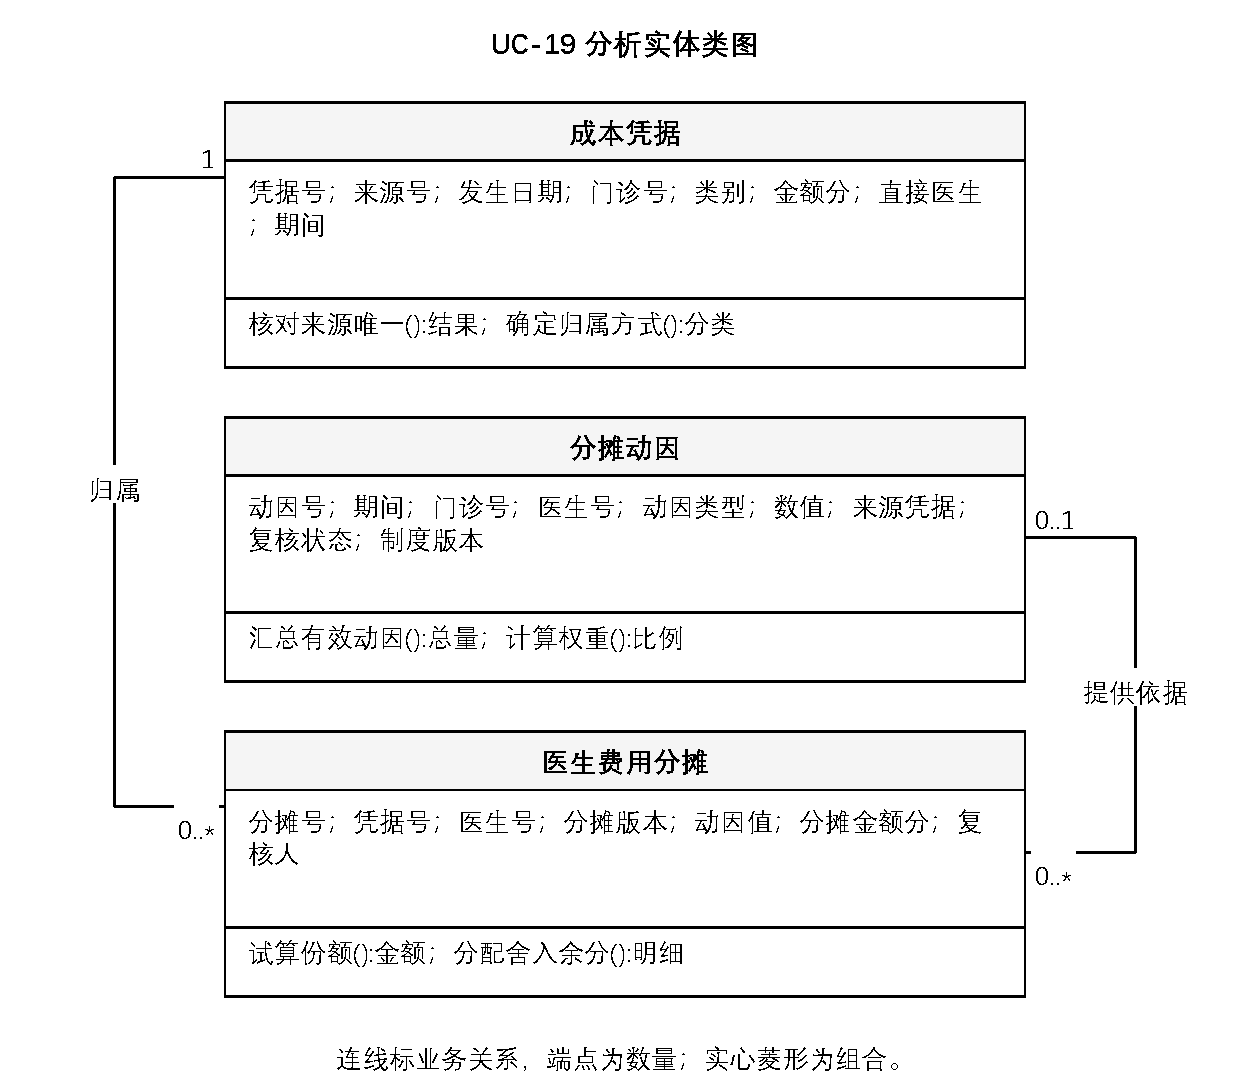
\includegraphics[width=\textwidth]{figures/class_UC_19.pdf}
\caption{UC-19 分析实体类图}\label{class_UC_19}\end{figure}
\begin{figure}[H]\centering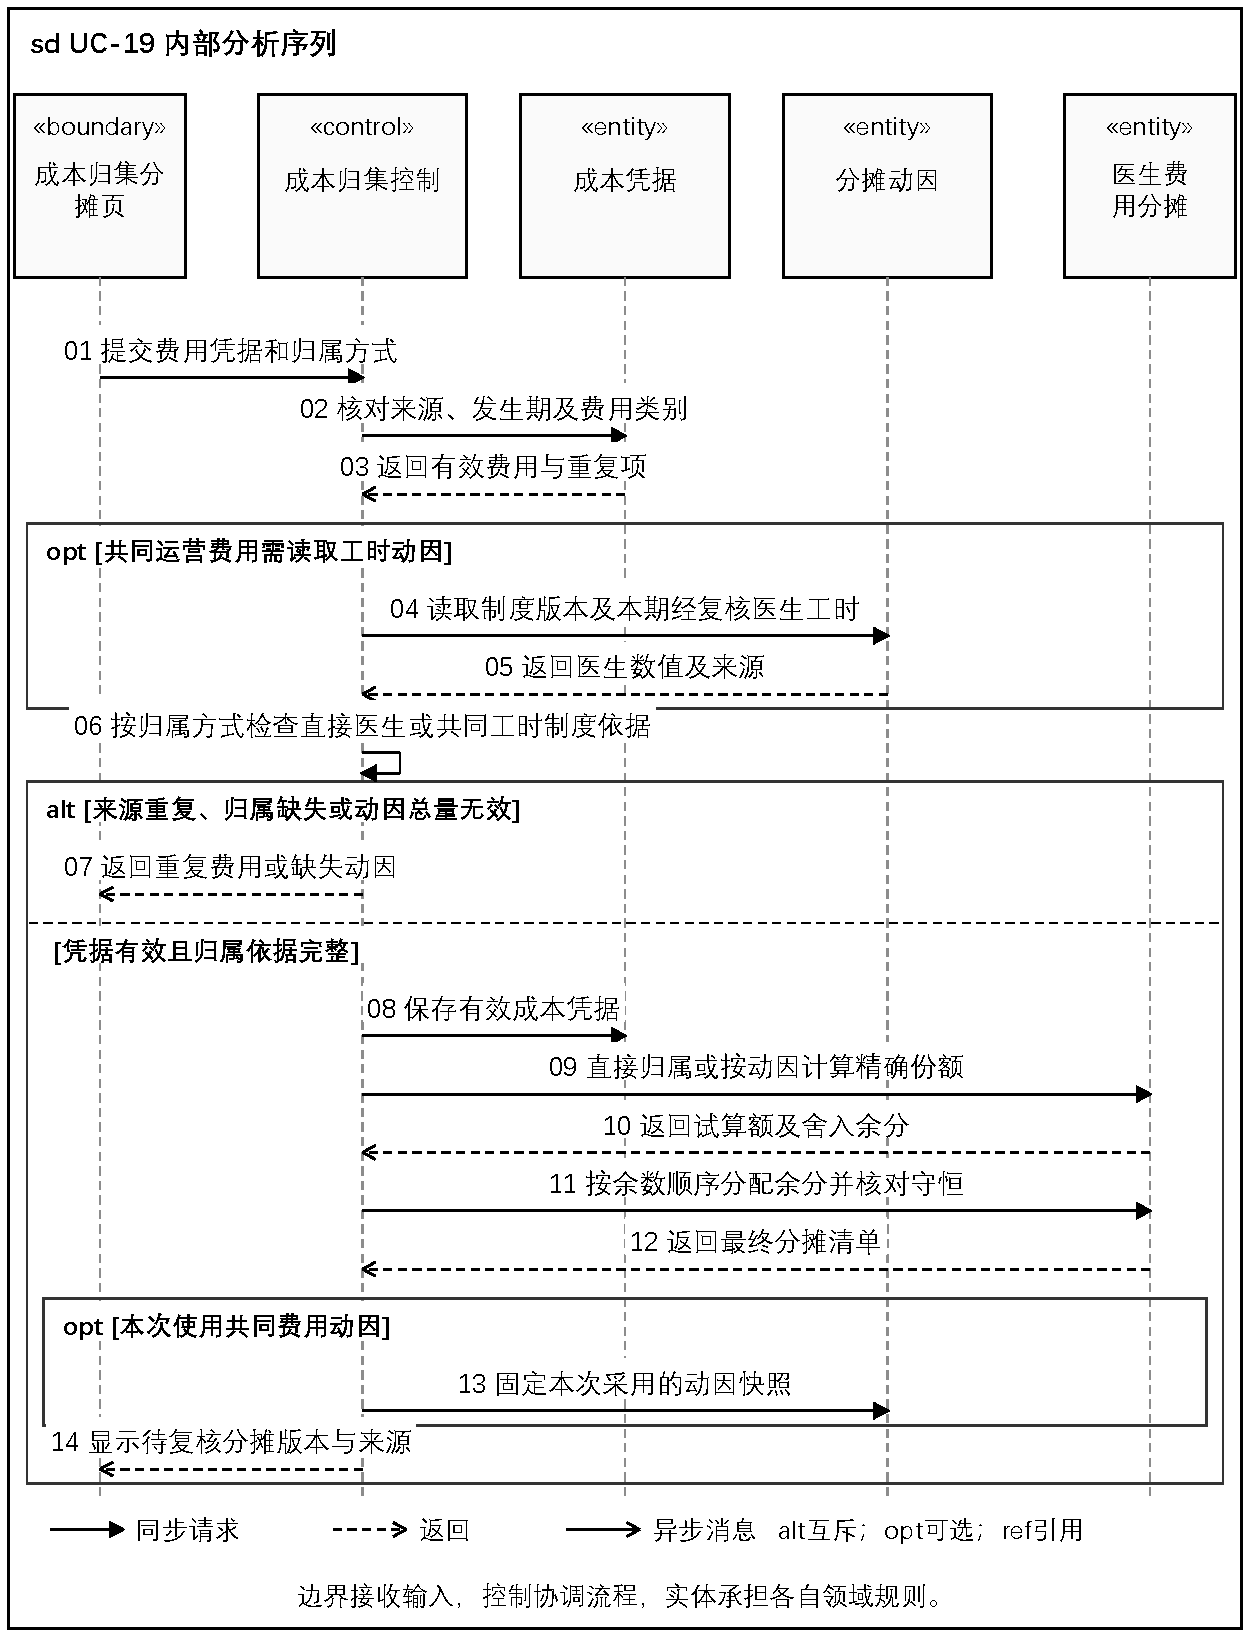
\includegraphics[width=\textwidth]{figures/seq_UC_19.pdf}
\caption{UC-19 内部分析序列}\label{seq_UC_19}\end{figure}
\par\noindent\begin{minipage}{\textwidth}
{\fontsize{10.5pt}{13.2pt}\selectfont\setlength{\tabcolsep}{0pt}\renewcommand{\arraystretch}{1.08}
\captionof{table}{UC-19操作契约 1}\label{tab339}
\begin{tabular}{@{}p{2.640cm}@{\hspace{0.16cm}}p{12.640cm}@{}}
\toprule
\bfseries \Cell{项目} & \bfseries \Cell{详细设计}\\\midrule
\Cell{签名} & \Cell{record\allowbreak{}Period\allowbreak{}Cost(\allowbreak{}source\allowbreak{}Id,\allowbreak{} cost\allowbreak{}Line,\allowbreak{} request\allowbreak{}Id)\allowbreak{}:\allowbreak{} Cost}\\[1pt]
\Cell{输入} & \Cell{类别、金额、耗用或费用凭据、门诊及日期}\\[1pt]
\Cell{执行前检查} & \Cell{凭据有效，期间开放，直接归属有依据}\\[1pt]
\Cell{成功结果} & \Cell{来源唯一的成本记录建立}\\[1pt]
\Cell{领域算法} & \Cell{以来源及行号查重；核对耗用而非付款日期口径，分开医疗用品与运营费用；直接归属记录医生，共同费用标待分摊。}\\[1pt]
\Cell{数据访问} & \Cell{成本仓储保存原金额与来源摘要；医生归属仓储保存直接费用明细。}\\[1pt]
\Cell{事务与并发} & \Cell{成本及直接归属原子保存；重复来源返回既有记录，凭据更正形成新版本或调整。}\\[1pt]
\Cell{失败及恢复} & \Cell{期间关闭转调整申请；来源不全退回补证；不生成无凭据成本。}\\[1pt]
\bottomrule\end{tabular}
}\end{minipage}\par\vspace{6pt}
\par\noindent\begin{minipage}{\textwidth}
{\fontsize{10.5pt}{13.2pt}\selectfont\setlength{\tabcolsep}{0pt}\renewcommand{\arraystretch}{1.08}
\captionof{table}{UC-19操作契约 2}\label{tab340}
\begin{tabular}{@{}p{2.640cm}@{\hspace{0.16cm}}p{12.640cm}@{}}
\toprule
\bfseries \Cell{项目} & \bfseries \Cell{详细设计}\\\midrule
\Cell{签名} & \Cell{allocate\allowbreak{}Common\allowbreak{}Cost(\allowbreak{}cost\allowbreak{}Id,\allowbreak{} driver\allowbreak{}Version,\allowbreak{} expected\allowbreak{}Cost\allowbreak{}Version)\allowbreak{}:\allowbreak{} Allocation}\\[1pt]
\Cell{输入} & \Cell{共同运营费用、经复核医生工时及适用制度版本}\\[1pt]
\Cell{执行前检查} & \Cell{默认工时动因非负且总量大于零；改用动因已有新制度批准}\\[1pt]
\Cell{成功结果} & \Cell{分摊守恒且可复算}\\[1pt]
\Cell{领域算法} & \Cell{按制度版本读取经复核医生工时，逐医生工时除以总量求精确份额；先取整数分，再按最大余数及稳定编号分配余分；核对守恒并固定工时来源及制度版本。}\\[1pt]
\Cell{数据访问} & \Cell{动因仓储读取来源快照；分摊仓储保存每名医生的比例、金额及版本。}\\[1pt]
\Cell{事务与并发} & \Cell{锁定成本版本，整组分摊和采用标记一次提交；不允许半组结果被季度读取。}\\[1pt]
\Cell{失败及恢复} & \Cell{工时缺失或总量为零停止；未批准的新动因不得采用；版本变化重算，失败保留原已确认版本。}\\[1pt]
\bottomrule\end{tabular}
}\end{minipage}\par\vspace{6pt}
\par\noindent\begin{minipage}{\textwidth}
{\fontsize{10.5pt}{13.2pt}\selectfont\setlength{\tabcolsep}{0pt}\renewcommand{\arraystretch}{1.08}
\captionof{table}{UC-19表示与验收}\label{tab341}
\begin{tabular}{@{}p{2.640cm}@{\hspace{0.16cm}}p{12.640cm}@{}}
\toprule
\bfseries \Cell{项目} & \bfseries \Cell{设计}\\\midrule
\Cell{界面} & \Cell{每笔费用可展开凭据、直接医生或分摊动因，显示合计差额与待补证项。}\\[1pt]
\Cell{接口} & \Cell{POST /\allowbreak{}period-\allowbreak{}costs；POST /\allowbreak{}period-\allowbreak{}costs/\allowbreak{}\{id\}/\allowbreak{}allocations；POST /\allowbreak{}cost-\allowbreak{}allocations/\allowbreak{}\{id\}/\allowbreak{}review。}\\[1pt]
\Cell{验收场景} & \Cell{1.\allowbreak{} 共同费用100分由三名等工时医生承担→34、33、33分且规则稳定。\\2.\allowbreak{} 同一来源重复登记→不重复扣成本。\\3.\allowbreak{} 动因为零→不产生随意均摊结果。\\4.\allowbreak{} 试算时擅自把工时改为收入权重→拒绝，须先批准新制度版本。}\\[1pt]
\bottomrule\end{tabular}
}\end{minipage}\par\vspace{6pt}
\Needspace{497pt}
\subsubsection{UC-20 复核经营期间并关账}
边界：经营期间关账页；控制：期间关账控制。\par
\begin{figure}[H]\centering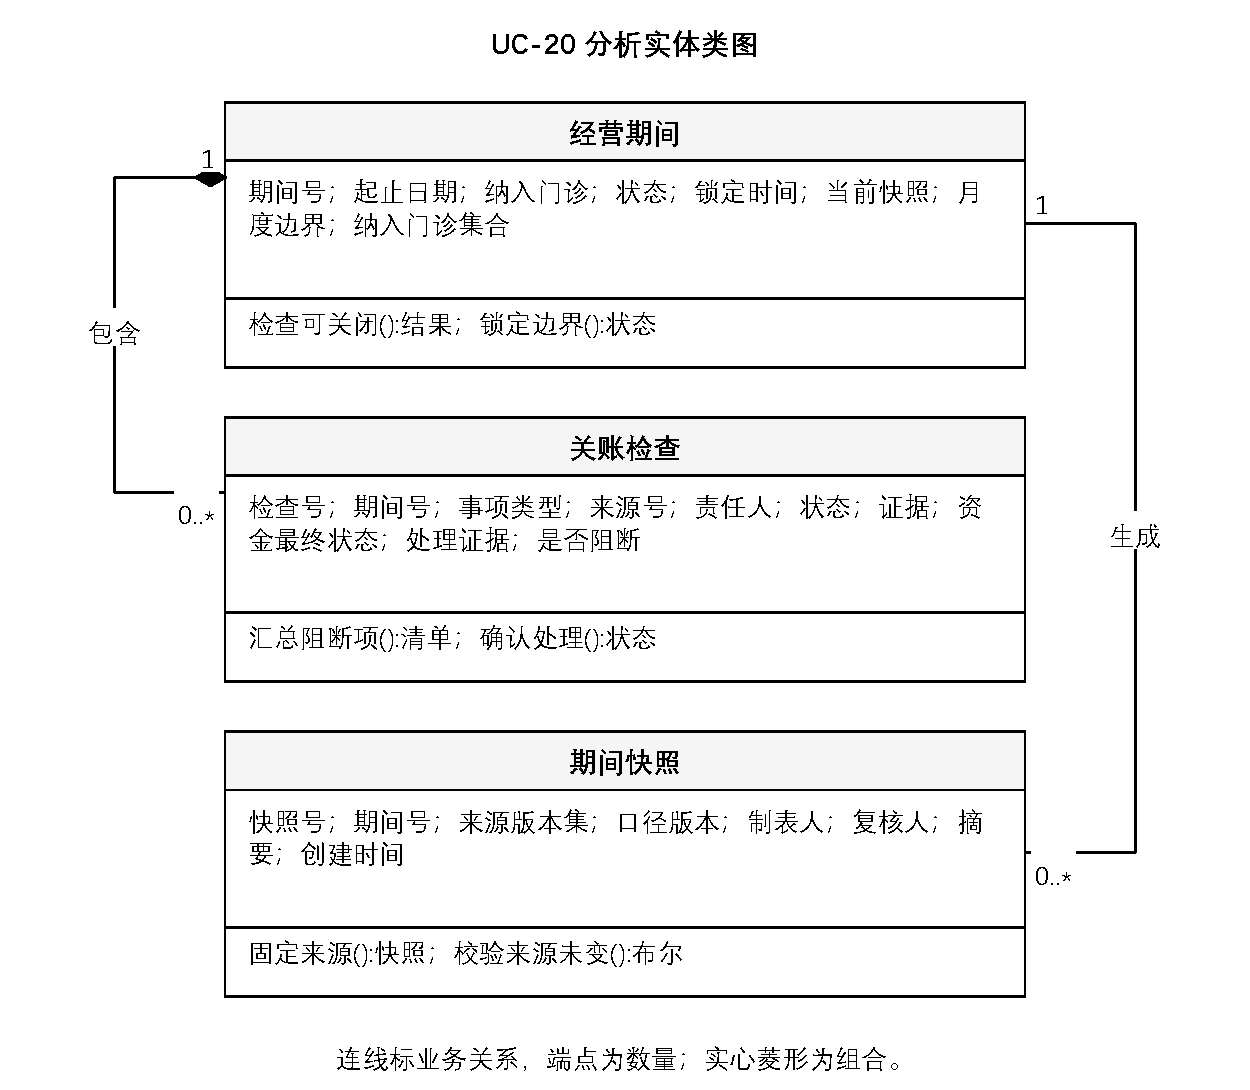
\includegraphics[width=\textwidth]{figures/class_UC_20.pdf}
\caption{UC-20 分析实体类图}\label{class_UC_20}\end{figure}
\begin{figure}[H]\centering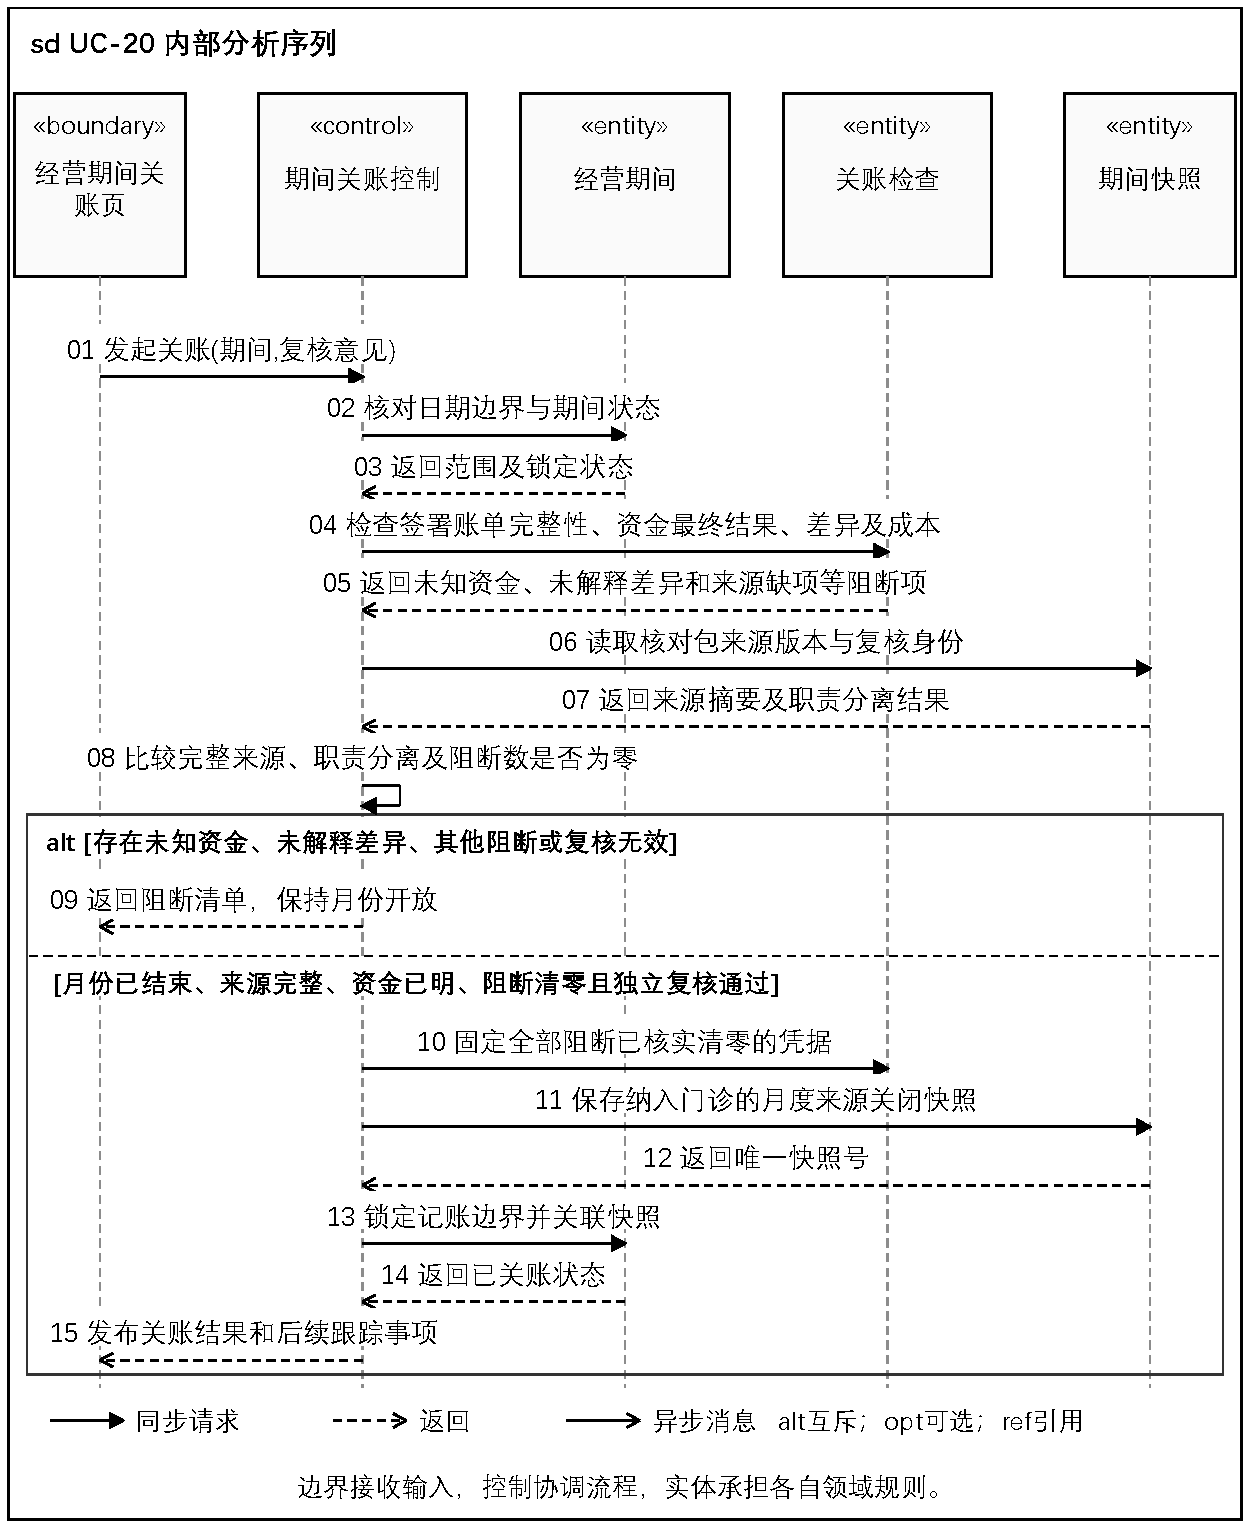
\includegraphics[width=\textwidth]{figures/seq_UC_20.pdf}
\caption{UC-20 内部分析序列}\label{seq_UC_20}\end{figure}
\par\noindent\begin{minipage}{\textwidth}
{\fontsize{10.5pt}{13.2pt}\selectfont\setlength{\tabcolsep}{0pt}\renewcommand{\arraystretch}{1.08}
\captionof{table}{UC-20操作契约 1}\label{tab346}
\begin{tabular}{@{}p{2.640cm}@{\hspace{0.16cm}}p{12.640cm}@{}}
\toprule
\bfseries \Cell{项目} & \bfseries \Cell{详细设计}\\\midrule
\Cell{签名} & \Cell{prepare\allowbreak{}Period\allowbreak{}Close(\allowbreak{}period\allowbreak{}Id)\allowbreak{}:\allowbreak{} Closing\allowbreak{}Package}\\[1pt]
\Cell{输入} & \Cell{自然月、组织有效范围及全部纳入门诊来源版本}\\[1pt]
\Cell{执行前检查} & \Cell{期间已结束且总部获授权}\\[1pt]
\Cell{成功结果} & \Cell{形成带阻断项的核对包}\\[1pt]
\Cell{领域算法} & \Cell{按月及组织有效期列应纳入门诊；检查已签执行与必要账单完整，按服务日和获准调整归集收入而不要求收清。逐店检查日结、收退款最终结果、资金及代收差异、成本分摊；任何未知结果或未解释差异均列阻断，正常欠款单列余额。}\\[1pt]
\Cell{数据访问} & \Cell{期间仓储读取边界；关账检查仓储保存逐项证据；快照仓储保存待复核包。}\\[1pt]
\Cell{事务与并发} & \Cell{按一致读取视图生成核对包；来源发生变化时标记包过期，不发布为已关账。}\\[1pt]
\Cell{失败及恢复} & \Cell{缺门诊、未签执行、缺账单、未知资金或未解释差异均阻断；读取失败不形成正式快照，不将缺失金额默认为零。}\\[1pt]
\bottomrule\end{tabular}
}\end{minipage}\par\vspace{6pt}
\par\noindent\begin{minipage}{\textwidth}
{\fontsize{10.5pt}{13.2pt}\selectfont\setlength{\tabcolsep}{0pt}\renewcommand{\arraystretch}{1.08}
\captionof{table}{UC-20操作契约 2}\label{tab347}
\begin{tabular}{@{}p{2.640cm}@{\hspace{0.16cm}}p{12.640cm}@{}}
\toprule
\bfseries \Cell{项目} & \bfseries \Cell{详细设计}\\\midrule
\Cell{签名} & \Cell{close\allowbreak{}Period(\allowbreak{}package\allowbreak{}Id,\allowbreak{} reviewer\allowbreak{}Id,\allowbreak{} expected\allowbreak{}Digest)\allowbreak{}:\allowbreak{} Period\allowbreak{}Snapshot}\\[1pt]
\Cell{输入} & \Cell{复核身份、意见和期望来源摘要}\\[1pt]
\Cell{执行前检查} & \Cell{月份已结束，全部来源完整且资金差异查清，阻断为零，制表与复核不同人}\\[1pt]
\Cell{成功结果} & \Cell{期间锁定且快照可引用}\\[1pt]
\Cell{领域算法} & \Cell{重新检查全部纳入门诊、来源摘要、资金最终状态及逐项处理证据；正常未收账款不要求清零。阻断数为零且复核有效后，原子固定月度收入成本及余额来源，写锁定边界和快照号。}\\[1pt]
\Cell{数据访问} & \Cell{快照仓储保存采用版本；期间仓储保存锁定；审计仓储保存复核结论。}\\[1pt]
\Cell{事务与并发} & \Cell{快照、期间锁定和审计同一短事务；任一版本冲突整体回滚。}\\[1pt]
\Cell{失败及恢复} & \Cell{资金未知或差异未解释保持开放；来源变化退回复核；重复关闭返回原快照；失败不得锁期却无快照。}\\[1pt]
\bottomrule\end{tabular}
}\end{minipage}\par\vspace{6pt}
\par\noindent\begin{minipage}{\textwidth}
{\fontsize{10.5pt}{13.2pt}\selectfont\setlength{\tabcolsep}{0pt}\renewcommand{\arraystretch}{1.08}
\captionof{table}{UC-20表示与验收}\label{tab348}
\begin{tabular}{@{}p{2.640cm}@{\hspace{0.16cm}}p{12.640cm}@{}}
\toprule
\bfseries \Cell{项目} & \bfseries \Cell{设计}\\\midrule
\Cell{界面} & \Cell{逐门诊显示月度来源、资金最终结果和阻断清单；正常应收及已确认往来单列，阻断未清时关闭按钮不可完成。}\\[1pt]
\Cell{接口} & \Cell{POST /\allowbreak{}periods/\allowbreak{}\{id\}/\allowbreak{}closing-\allowbreak{}package；POST /\allowbreak{}closing-\allowbreak{}packages/\allowbreak{}\{id\}/\allowbreak{}close。}\\[1pt]
\Cell{验收场景} & \Cell{1.\allowbreak{} 签署执行及账单500元已出具，患者仅付300元且核对齐全→可关账，收入500元和应收200元分别保留。\\2.\allowbreak{} 退款仍在途且结果未知→即使有责任人与查证计划也不能关账。\\3.\allowbreak{} 成本未分摊或必要账单缺失→阻断关闭。\\4.\allowbreak{} 关闭提交时来源变化→保持开放并重新复核。}\\[1pt]
\bottomrule\end{tabular}
}\end{minipage}\par\vspace{6pt}
\Needspace{497pt}
\subsubsection{UC-21 计算医生季度业绩及10\%激励基金}
边界：季度业绩试算页；控制：季度业绩计算控制。\par
\begin{figure}[H]\centering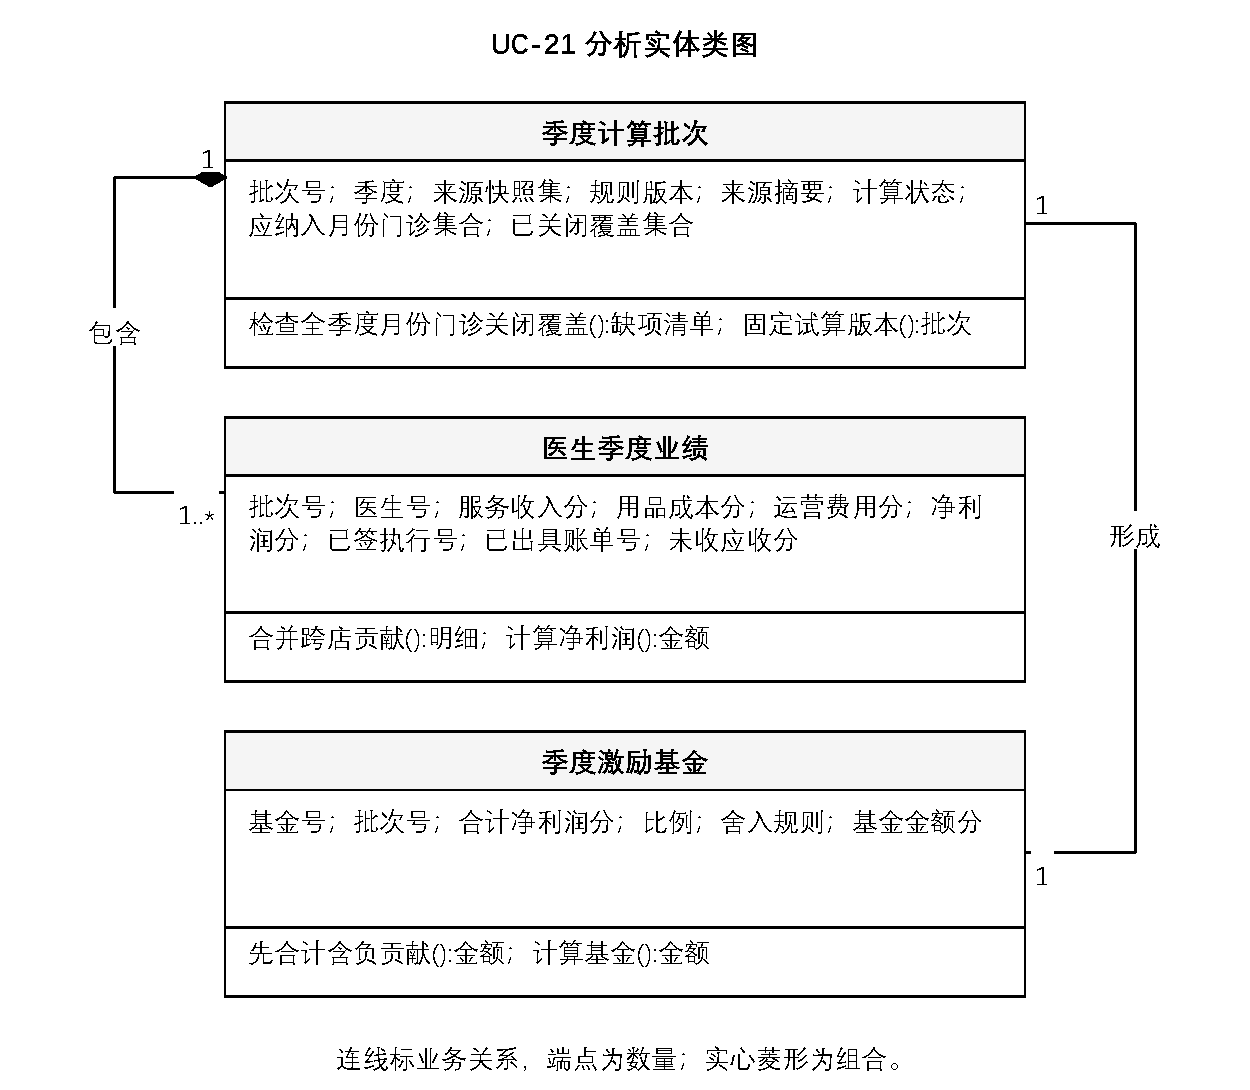
\includegraphics[width=\textwidth]{figures/class_UC_21.pdf}
\caption{UC-21 分析实体类图}\label{class_UC_21}\end{figure}
\begin{figure}[H]\centering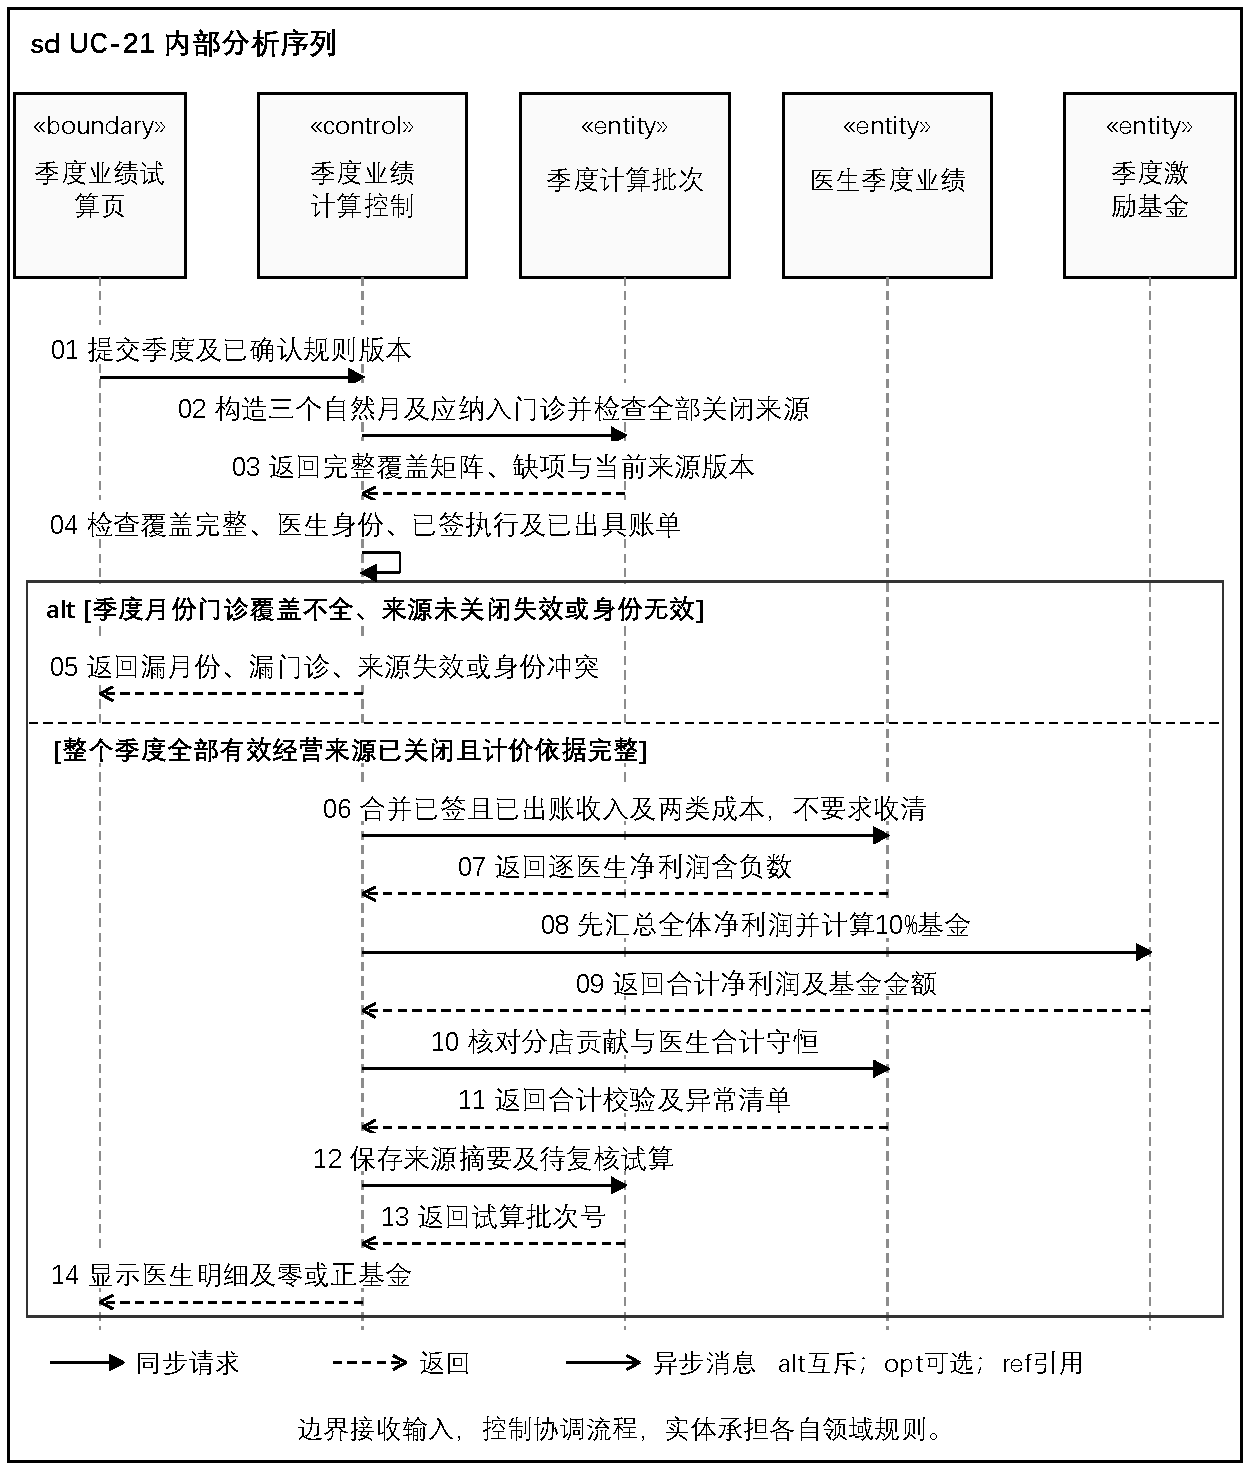
\includegraphics[width=\textwidth]{figures/seq_UC_21.pdf}
\caption{UC-21 内部分析序列}\label{seq_UC_21}\end{figure}
\par\noindent\begin{minipage}{\textwidth}
{\fontsize{10.5pt}{13.2pt}\selectfont\setlength{\tabcolsep}{0pt}\renewcommand{\arraystretch}{1.08}
\captionof{table}{UC-21操作契约}\label{tab353}
\begin{tabular}{@{}p{2.640cm}@{\hspace{0.16cm}}p{12.640cm}@{}}
\toprule
\bfseries \Cell{项目} & \bfseries \Cell{详细设计}\\\midrule
\Cell{签名} & \Cell{calculate\allowbreak{}Quarter\allowbreak{}Performance(\allowbreak{}quarter\allowbreak{}Id,\allowbreak{} snapshot\allowbreak{}Ids,\allowbreak{} rule\allowbreak{}Version)\allowbreak{}:\allowbreak{} Quarter\allowbreak{}Trial}\\[1pt]
\Cell{输入} & \Cell{季度号、规则版本；完整来源由服务端按组织有效期确定}\\[1pt]
\Cell{执行前检查} & \Cell{三个自然月及全部应纳入门诊均有有效关闭快照，执行签署和账单齐全，成本完整}\\[1pt]
\Cell{成功结果} & \Cell{可复算的医生净利润与基金试算建立}\\[1pt]
\Cell{领域算法} & \Cell{先按季度日期及组织有效期生成应纳入月份门诊矩阵，与当前关闭快照逐项核对，缺失或失效立即停止；不得接受部分来源子集。按已签执行及已出具账单去重归集收入，不要求收清；跨店合并实际医生与有效调整，扣除两类已复核成本。先合计含负数净利润，再取与零较大者乘10\%，四舍五入至分。}\\[1pt]
\Cell{数据访问} & \Cell{期间快照仓储按季度全范围读取当前关闭来源；季度仓储固定覆盖集合、医生明细及各店展开；基金仓储保存公式输入。}\\[1pt]
\Cell{事务与并发} & \Cell{同一来源摘要和规则唯一创建试算，医生行、基金及校验一起提交；失败不发布部分结果。}\\[1pt]
\Cell{失败及恢复} & \Cell{漏月份、漏门诊、来源失效或未签未出账停止；正常未收应收不当作缺收入；零负合计正常生成零基金，重试返回原试算。}\\[1pt]
\bottomrule\end{tabular}
}\end{minipage}\par\vspace{6pt}
\par\noindent\begin{minipage}{\textwidth}
{\fontsize{10.5pt}{13.2pt}\selectfont\setlength{\tabcolsep}{0pt}\renewcommand{\arraystretch}{1.08}
\captionof{table}{UC-21表示与验收}\label{tab354}
\begin{tabular}{@{}p{2.640cm}@{\hspace{0.16cm}}p{12.640cm}@{}}
\toprule
\bfseries \Cell{项目} & \bfseries \Cell{设计}\\\midrule
\Cell{界面} & \Cell{先展示三个月与门诊关闭覆盖矩阵；通过完整性检查后显示医生跨店明细、未收应收和基金计算式。}\\[1pt]
\Cell{接口} & \Cell{POST /\allowbreak{}quarters/\allowbreak{}\{id\}/\allowbreak{}performance-\allowbreak{}trials；GET /\allowbreak{}performance-\allowbreak{}trials/\allowbreak{}\{id\}/\allowbreak{}sources。}\\[1pt]
\Cell{验收场景} & \Cell{1.\allowbreak{} 医生A净利润12000元、B亏损2000元→合计10000元，基金1000元。\\2.\allowbreak{} 同一医生跨两店→形成同一医生汇总且保留两店展开。\\3.\allowbreak{} 合计净利润为负→基金为零，亏损行不删除。\\4.\allowbreak{} 只提交季度中两个月的有效快照→仍拒绝，指出缺少的月份及门诊。\\5.\allowbreak{} 其中一家有效门诊缺快照→不能按零成本零收入继续。\\6.\allowbreak{} 已签执行且已出具500元账单，仅收300元→季度收入采用500元，应收200元另列。}\\[1pt]
\bottomrule\end{tabular}
}\end{minipage}\par\vspace{6pt}
\Needspace{497pt}
\subsubsection{UC-22 复核激励分配并登记发放}
边界：激励分配发放页；控制：激励分配控制。\par
\begin{figure}[H]\centering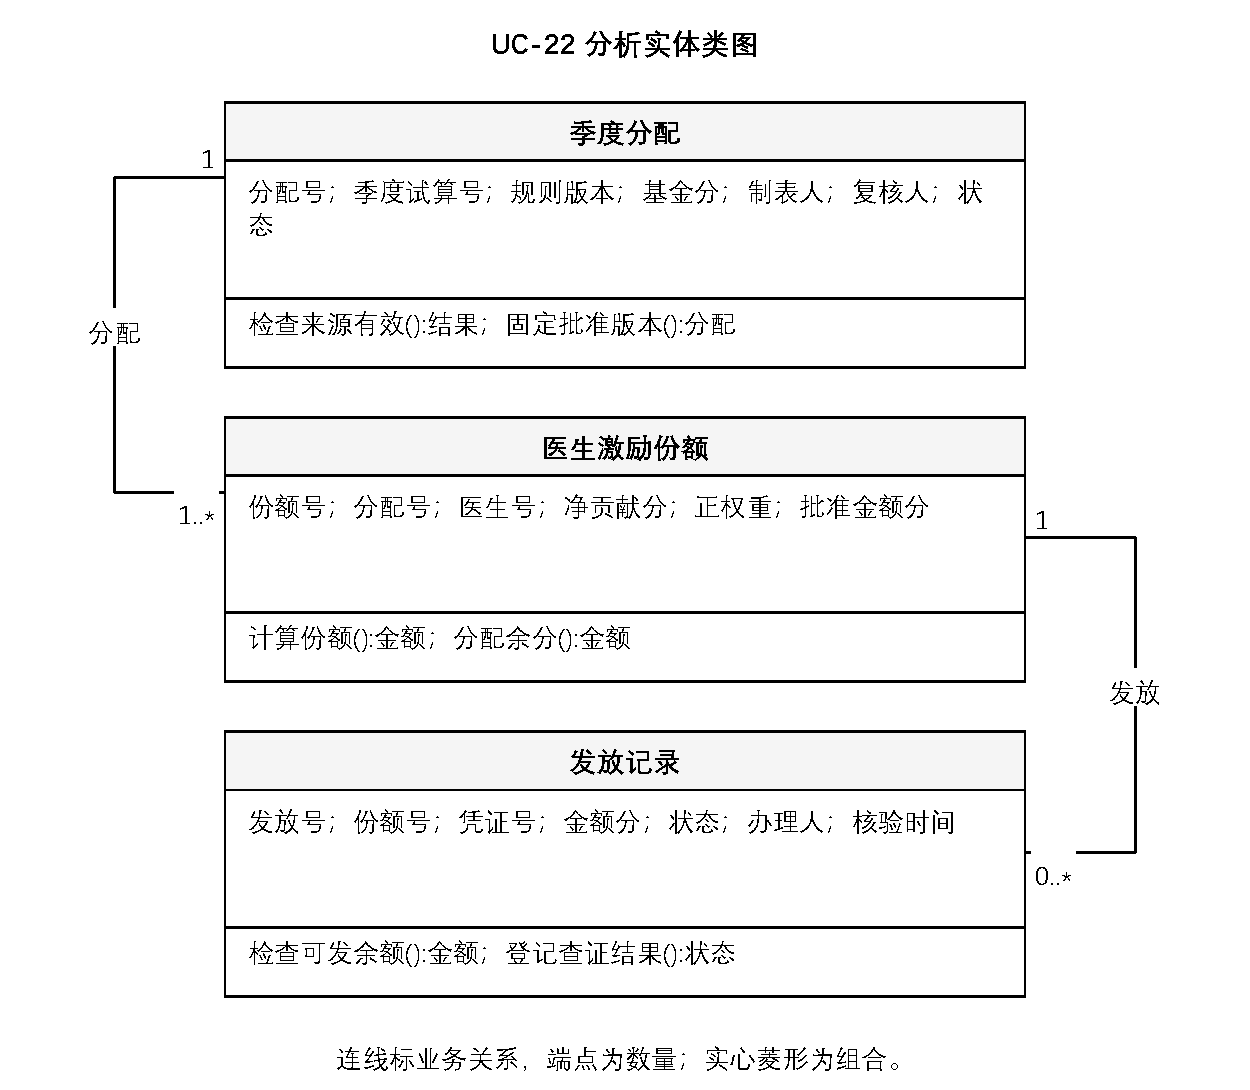
\includegraphics[width=\textwidth]{figures/class_UC_22.pdf}
\caption{UC-22 分析实体类图}\label{class_UC_22}\end{figure}
\begin{figure}[H]\centering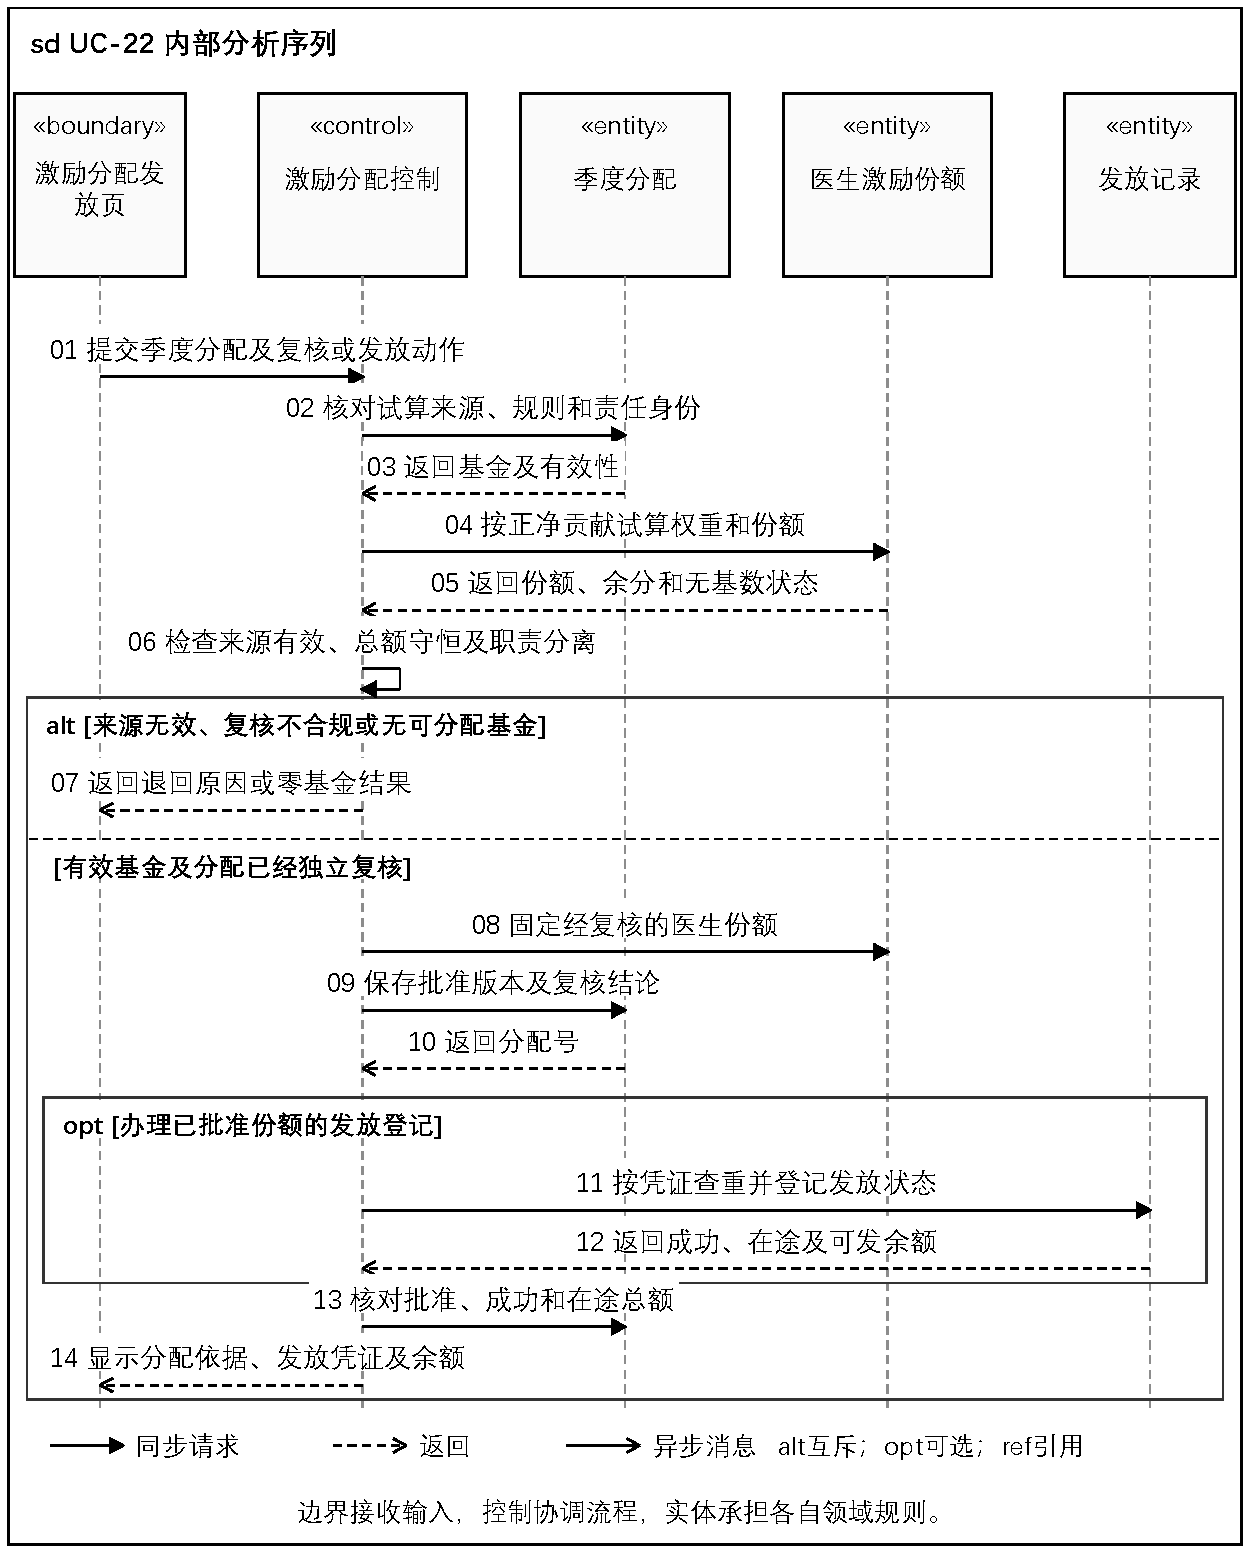
\includegraphics[width=\textwidth]{figures/seq_UC_22.pdf}
\caption{UC-22 内部分析序列}\label{seq_UC_22}\end{figure}
\par\noindent\begin{minipage}{\textwidth}
{\fontsize{10.5pt}{13.2pt}\selectfont\setlength{\tabcolsep}{0pt}\renewcommand{\arraystretch}{1.08}
\captionof{table}{UC-22操作契约 1}\label{tab359}
\begin{tabular}{@{}p{2.640cm}@{\hspace{0.16cm}}p{12.640cm}@{}}
\toprule
\bfseries \Cell{项目} & \bfseries \Cell{详细设计}\\\midrule
\Cell{签名} & \Cell{approve\allowbreak{}Incentive\allowbreak{}Distribution(\allowbreak{}trial\allowbreak{}Id,\allowbreak{} reviewer\allowbreak{}Id,\allowbreak{} expected\allowbreak{}Digest)\allowbreak{}:\allowbreak{} Distribution}\\[1pt]
\Cell{输入} & \Cell{有效试算、复核意见及来源摘要}\\[1pt]
\Cell{执行前检查} & \Cell{制表与复核不同人，规则已确认}\\[1pt]
\Cell{成功结果} & \Cell{基金守恒的医生份额固定}\\[1pt]
\Cell{领域算法} & \Cell{重新核对含负数合计的基金；对正净贡献求权重，取整数分后按最大余数稳定分配余分；无基数不分配。复核者查看每行后确认。}\\[1pt]
\Cell{数据访问} & \Cell{季度仓储读取试算；分配及份额仓储保存基金、权重、余差与批准版本。}\\[1pt]
\Cell{事务与并发} & \Cell{整组份额、批准结论和来源引用同一事务提交；任一校验失败均不发布。}\\[1pt]
\Cell{失败及恢复} & \Cell{来源重开导致失效则退回重算；同版本重复批准返回原分配；拒绝擅改权重。}\\[1pt]
\bottomrule\end{tabular}
}\end{minipage}\par\vspace{6pt}
\par\noindent\begin{minipage}{\textwidth}
{\fontsize{10.5pt}{13.2pt}\selectfont\setlength{\tabcolsep}{0pt}\renewcommand{\arraystretch}{1.08}
\captionof{table}{UC-22操作契约 2}\label{tab360}
\begin{tabular}{@{}p{2.640cm}@{\hspace{0.16cm}}p{12.640cm}@{}}
\toprule
\bfseries \Cell{项目} & \bfseries \Cell{详细设计}\\\midrule
\Cell{签名} & \Cell{record\allowbreak{}Incentive\allowbreak{}Payment(\allowbreak{}share\allowbreak{}Id,\allowbreak{} voucher,\allowbreak{} status,\allowbreak{} amount)\allowbreak{}:\allowbreak{} Payout}\\[1pt]
\Cell{输入} & \Cell{批准份额、核实凭证、金额和状态}\\[1pt]
\Cell{执行前检查} & \Cell{批准有效，办理人有发放权限}\\[1pt]
\Cell{成功结果} & \Cell{可发余额与凭证一致，无超额登记}\\[1pt]
\Cell{领域算法} & \Cell{以凭证号查重，锁定该医生批准份额，扣除已成功与在途占用后检查余额；成功才确认支出，失败释放占用，不明保持在途。}\\[1pt]
\Cell{数据访问} & \Cell{发放仓储记录状态及核验依据；份额仓储保存成功和在途累计。}\\[1pt]
\Cell{事务与并发} & \Cell{记录、额度占用和累计额原子更新；外部付款查证在事务外进行。}\\[1pt]
\Cell{失败及恢复} & \Cell{同凭证不同金额进入核验；超发拒绝；状态未知不得重复支付或释放占用。}\\[1pt]
\bottomrule\end{tabular}
}\end{minipage}\par\vspace{6pt}
\par\noindent\begin{minipage}{\textwidth}
{\fontsize{10.5pt}{13.2pt}\selectfont\setlength{\tabcolsep}{0pt}\renewcommand{\arraystretch}{1.08}
\captionof{table}{UC-22表示与验收}\label{tab361}
\begin{tabular}{@{}p{2.640cm}@{\hspace{0.16cm}}p{12.640cm}@{}}
\toprule
\bfseries \Cell{项目} & \bfseries \Cell{设计}\\\midrule
\Cell{界面} & \Cell{展示基金计算、医生正负贡献、批准份额和发放状态；个人视图只见本人份额依据。}\\[1pt]
\Cell{接口} & \Cell{POST /\allowbreak{}performance-\allowbreak{}trials/\allowbreak{}\{id\}/\allowbreak{}distribution-\allowbreak{}review；POST /\allowbreak{}incentive-\allowbreak{}shares/\allowbreak{}\{id\}/\allowbreak{}payouts。}\\[1pt]
\Cell{验收场景} & \Cell{1.\allowbreak{} 一名亏损医生→其分配权重为零，但亏损已降低基金。\\2.\allowbreak{} 四舍五入产生余分→最终分配合计与基金完全一致。\\3.\allowbreak{} 同一凭证重复登记→只有一笔发放。}\\[1pt]
\bottomrule\end{tabular}
}\end{minipage}\par\vspace{6pt}
\Needspace{497pt}
\subsubsection{UC-23 分析取消率与技能供需}
边界：预约技能分析页；控制：预约技能分析控制。\par
\begin{figure}[H]\centering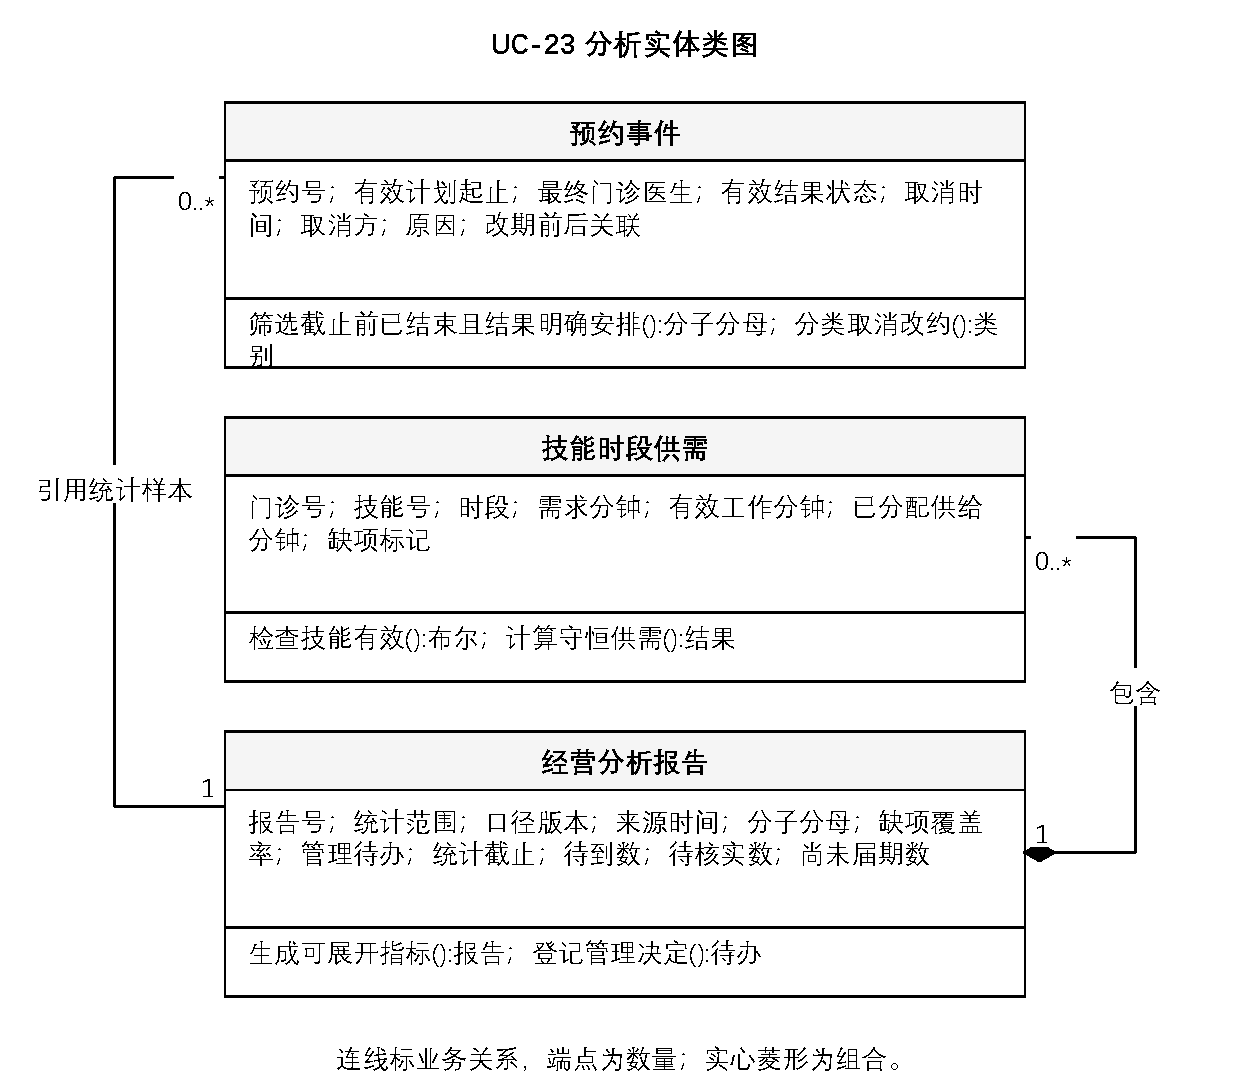
\includegraphics[width=\textwidth]{figures/class_UC_23.pdf}
\caption{UC-23 分析实体类图}\label{class_UC_23}\end{figure}
\begin{figure}[H]\centering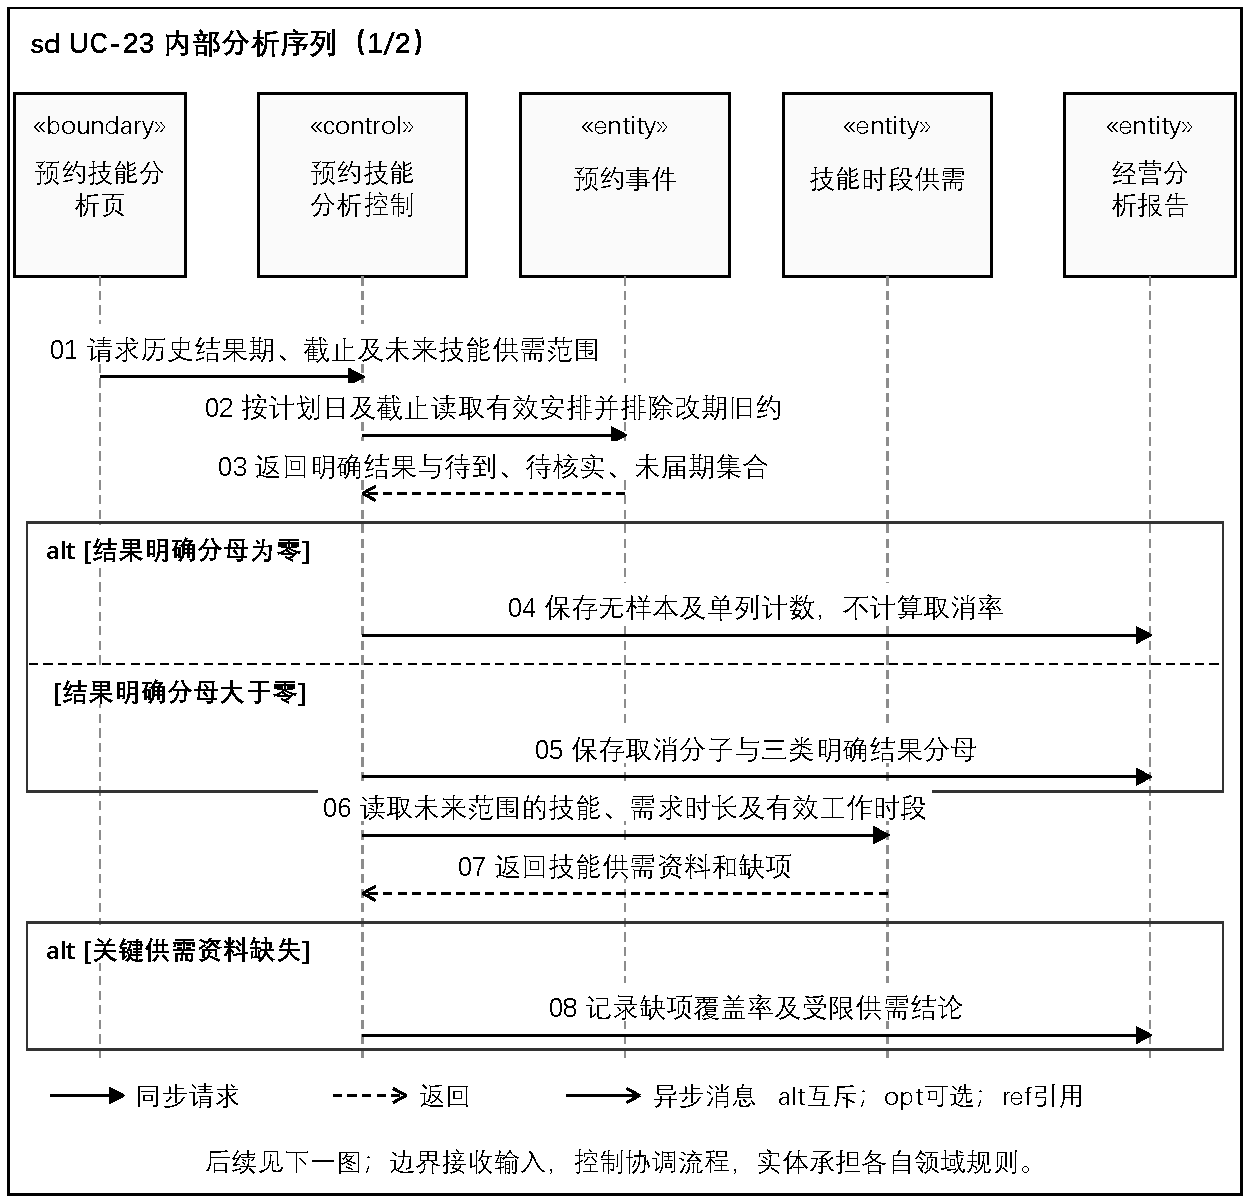
\includegraphics[width=\textwidth]{figures/seq_UC_23_1.pdf}
\caption{UC-23 内部分析序列（1/2）}\label{seq_UC_23_1}\end{figure}
\begin{figure}[H]\centering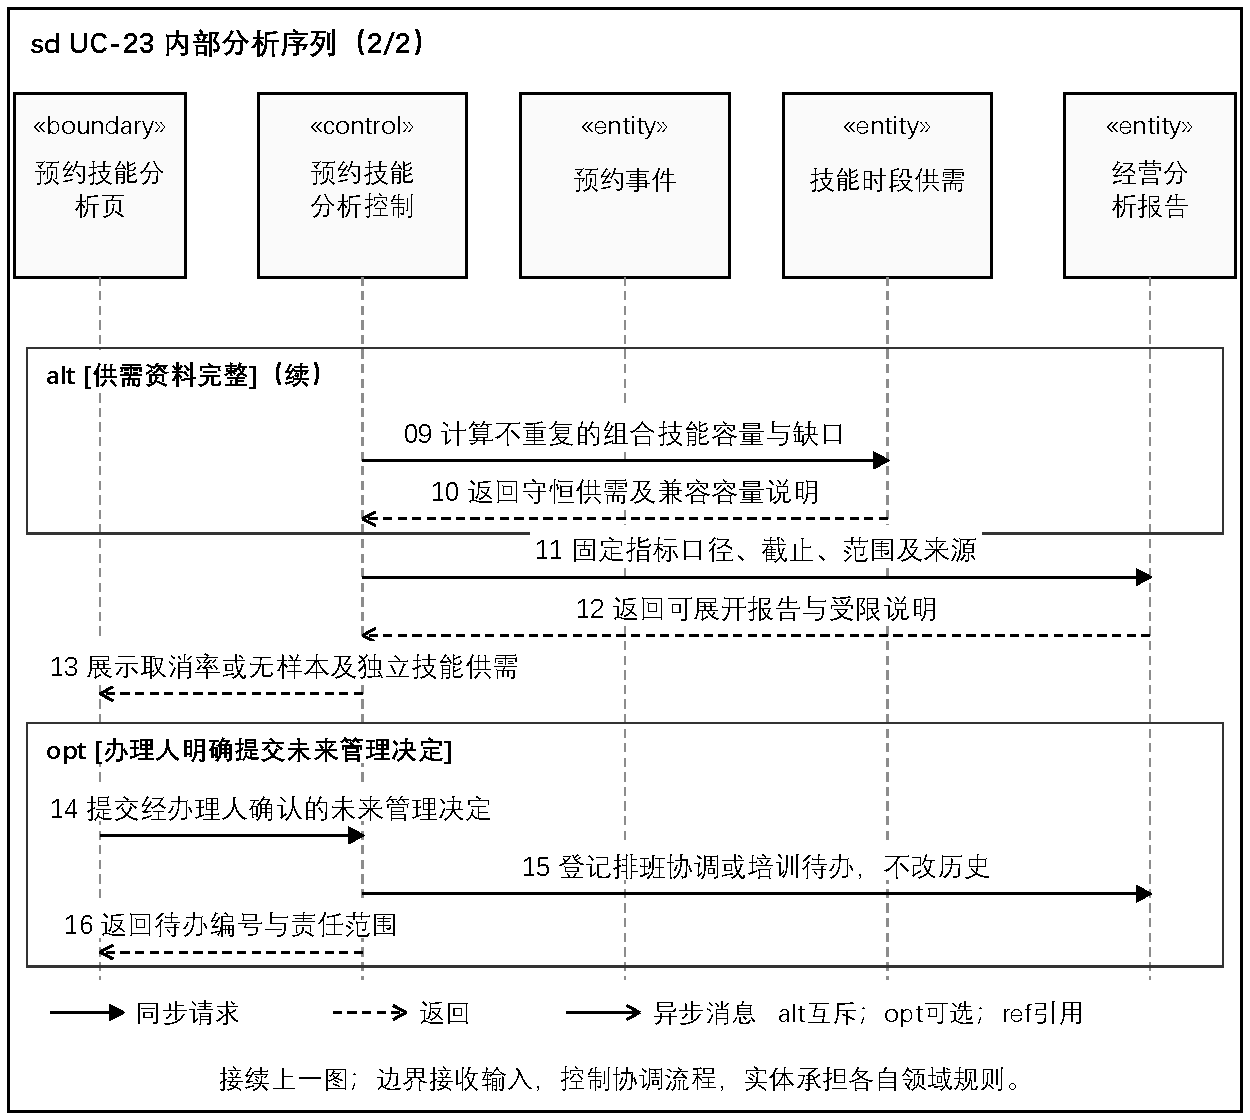
\includegraphics[width=\textwidth]{figures/seq_UC_23_2.pdf}
\caption{UC-23 内部分析序列（2/2）}\label{seq_UC_23_2}\end{figure}
\par\noindent\begin{minipage}{\textwidth}
{\fontsize{10.5pt}{13.2pt}\selectfont\setlength{\tabcolsep}{0pt}\renewcommand{\arraystretch}{1.08}
\captionof{table}{UC-23操作契约}\label{tab367}
\begin{tabular}{@{}p{2.640cm}@{\hspace{0.16cm}}p{12.640cm}@{}}
\toprule
\bfseries \Cell{项目} & \bfseries \Cell{详细设计}\\\midrule
\Cell{签名} & \Cell{analyze\allowbreak{}Appointment\allowbreak{}And\allowbreak{}Skills(\allowbreak{}scope,\allowbreak{} period,\allowbreak{} metric\allowbreak{}Version)\allowbreak{}:\allowbreak{} Report}\\[1pt]
\Cell{输入} & \Cell{计划日期范围、统计截止、门诊技能范围和固定指标定义}\\[1pt]
\Cell{执行前检查} & \Cell{办理者有范围权限，正式取消率只取截止前已结束的明确结果}\\[1pt]
\Cell{成功结果} & \Cell{来源可展开、缺项透明的统计报告形成}\\[1pt]
\Cell{领域算法} & \Cell{按当前有效安排的计划日与最终门诊医生归组，排除改期旧约和临时占位；筛选截止前已结束且状态为已到诊、已取消或已确认未到的集合，分母为三者合计，分子为已取消。待到、待核实和未来未决单列，零分母显示无样本。未来技能供需另按明确时间范围计算，候补去重，多技能医生组合容量守恒。}\\[1pt]
\Cell{数据访问} & \Cell{预约事件仓储按计划日、有效改期链、截止和结果状态读取；排班技能仓储按未来供需范围查询；报告仓储固定口径、截止及来源。}\\[1pt]
\Cell{事务与并发} & \Cell{一致读取生成报告快照；仅写报告及人工确认的待办，不修改预约或排班事实。}\\[1pt]
\Cell{失败及恢复} & \Cell{结果明确分母为零显示无样本，即使有未来预约；资料缺失显示覆盖率，不把未知状态补成取消或到诊。}\\[1pt]
\bottomrule\end{tabular}
}\end{minipage}\par\vspace{6pt}
\par\noindent\begin{minipage}{\textwidth}
{\fontsize{10.5pt}{13.2pt}\selectfont\setlength{\tabcolsep}{0pt}\renewcommand{\arraystretch}{1.08}
\captionof{table}{UC-23表示与验收}\label{tab368}
\begin{tabular}{@{}p{2.640cm}@{\hspace{0.16cm}}p{12.640cm}@{}}
\toprule
\bfseries \Cell{项目} & \bfseries \Cell{设计}\\\midrule
\Cell{界面} & \Cell{同时显示明确结果的三类计数、待到/\allowbreak{}待核实/\allowbreak{}未来未决及取消率；技能供需采用单独标明的未来范围。}\\[1pt]
\Cell{接口} & \Cell{GET /\allowbreak{}reports/\allowbreak{}appointment-\allowbreak{}skill-\allowbreak{}demand；POST /\allowbreak{}reports/\allowbreak{}\{id\}/\allowbreak{}management-\allowbreak{}actions。}\\[1pt]
\Cell{验收场景} & \Cell{1.\allowbreak{} 已到诊8、已取消2、已确认未到1，另有待到4及待核实3→分母11，取消率2/\allowbreak{}11。\\2.\allowbreak{} 只有未来待到预约→无样本，不显示0\%。\\3.\allowbreak{} 改期旧约→保留历史但不重复计分母，新约按其有效计划日和最终结果统计。\\4.\allowbreak{} 同一医生双技能仅60分钟→组合供给不超过60分钟。}\\[1pt]
\bottomrule\end{tabular}
}\end{minipage}\par\vspace{6pt}
\Needspace{608pt}
\subsubsection{UC-24 维护门诊组织和岗位授权}
边界：组织岗位授权页；控制：组织授权控制。\par
\begin{figure}[H]\centering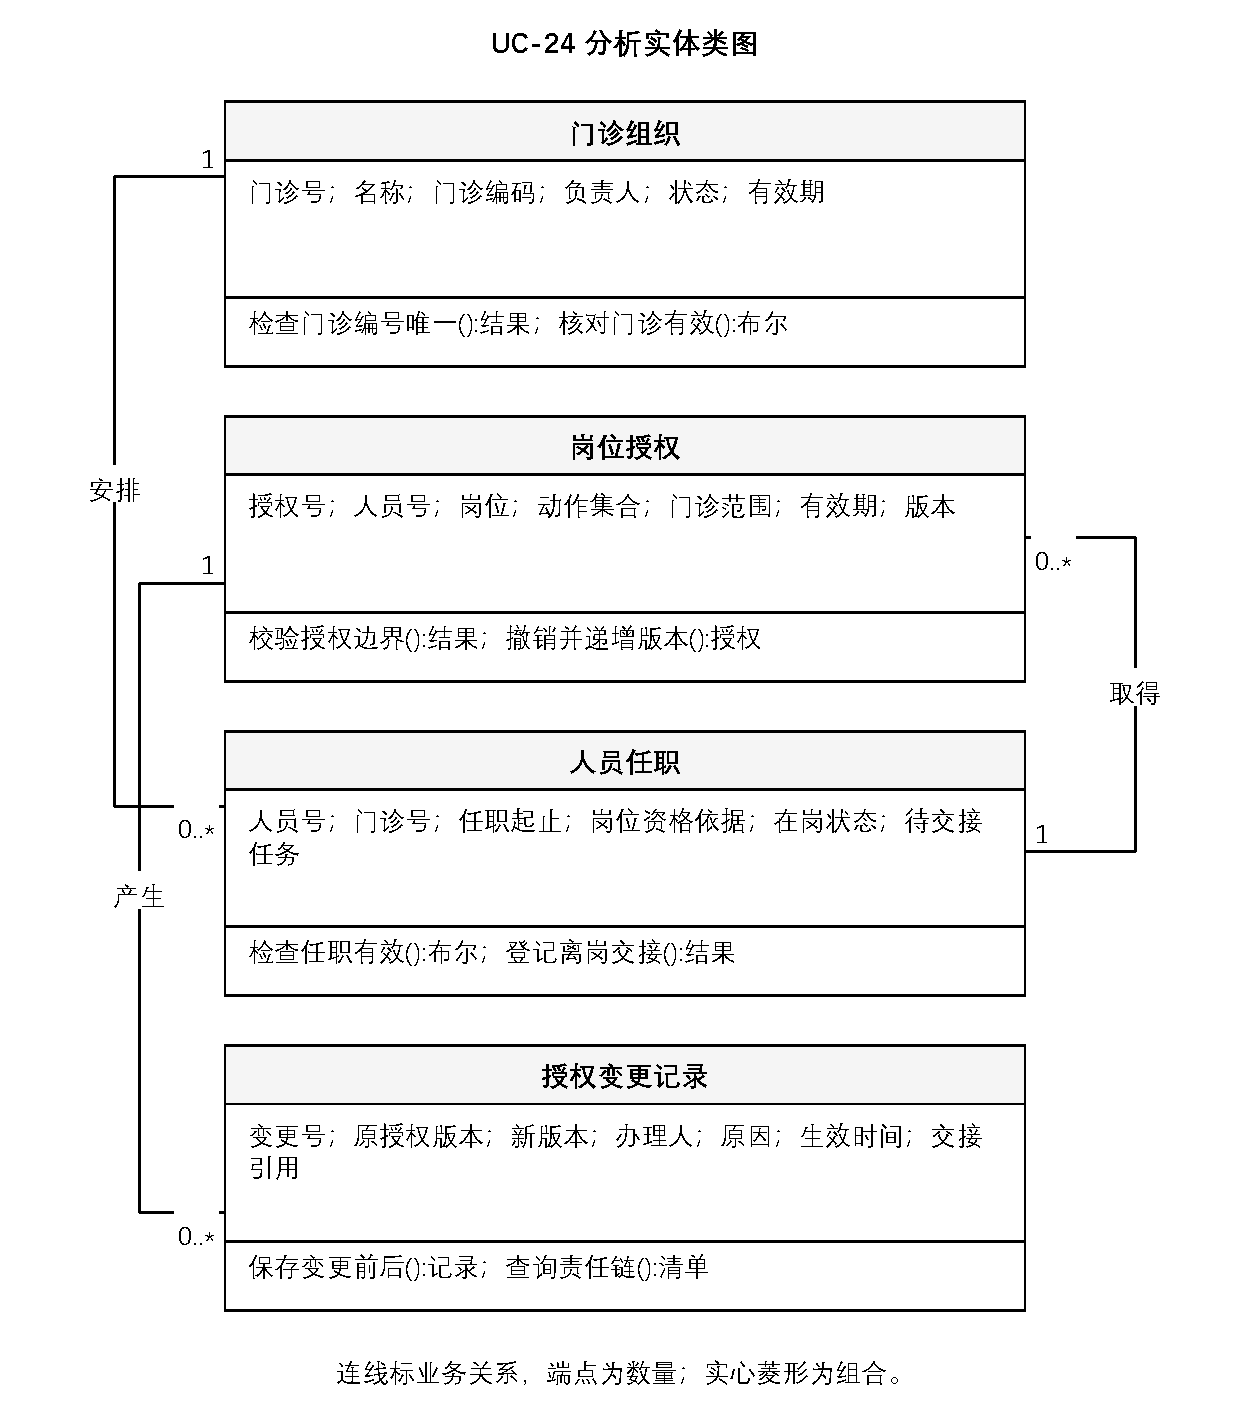
\includegraphics[width=\textwidth]{figures/class_UC_24.pdf}
\caption{UC-24 分析实体类图}\label{class_UC_24}\end{figure}
\begin{figure}[H]\centering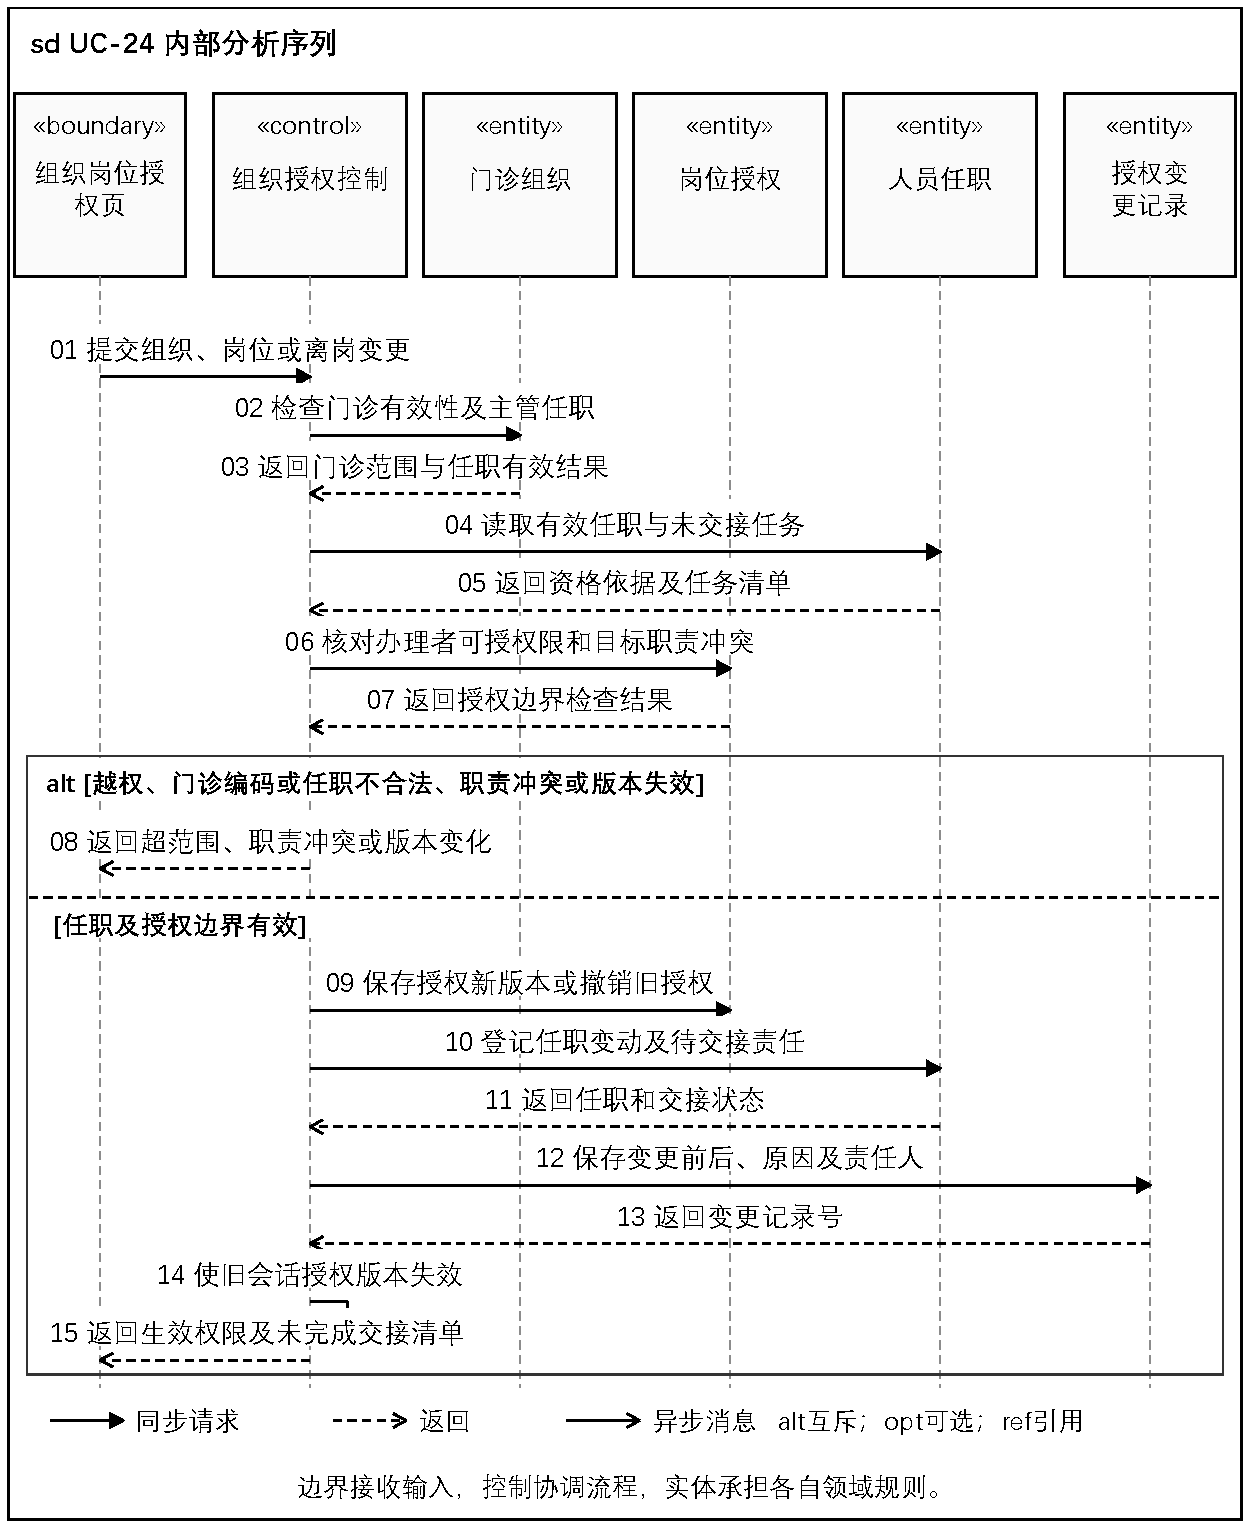
\includegraphics[width=\textwidth]{figures/seq_UC_24.pdf}
\caption{UC-24 内部分析序列}\label{seq_UC_24}\end{figure}
\par\noindent\begin{minipage}{\textwidth}
{\fontsize{10.5pt}{13.2pt}\selectfont\setlength{\tabcolsep}{0pt}\renewcommand{\arraystretch}{1.08}
\captionof{table}{UC-24操作契约 1}\label{tab373}
\begin{tabular}{@{}p{2.640cm}@{\hspace{0.16cm}}p{12.640cm}@{}}
\toprule
\bfseries \Cell{项目} & \bfseries \Cell{详细设计}\\\midrule
\Cell{签名} & \Cell{change\allowbreak{}Assignment(\allowbreak{}person\allowbreak{}Id,\allowbreak{} role,\allowbreak{} scope,\allowbreak{} validity,\allowbreak{} expected\allowbreak{}Version)\allowbreak{}:\allowbreak{} Grant}\\[1pt]
\Cell{输入} & \Cell{人员、岗位、门诊范围、有效期及理由}\\[1pt]
\Cell{执行前检查} & \Cell{办理者有可授权限，任职依据有效}\\[1pt]
\Cell{成功结果} & \Cell{权限版本更新且可追溯}\\[1pt]
\Cell{领域算法} & \Cell{核对门诊编码唯一及主管有效、任职有效期和可授动作；检查总部制表复核职责冲突及店长范围，不把岗位授予等同技能认证；展示差异后原子更新授权版本。}\\[1pt]
\Cell{数据访问} & \Cell{组织及任职仓储核对范围；授权仓储保存有效版本；变更仓储保存前后快照。}\\[1pt]
\Cell{事务与并发} & \Cell{授权、任职和变更记录同一事务提交；后续每次操作比较当前权限版本。}\\[1pt]
\Cell{失败及恢复} & \Cell{超范围整单拒绝；并发授权冲突要求重读；失效账号的旧会话不能继续操作。}\\[1pt]
\bottomrule\end{tabular}
}\end{minipage}\par\vspace{6pt}
\par\noindent\begin{minipage}{\textwidth}
{\fontsize{10.5pt}{13.2pt}\selectfont\setlength{\tabcolsep}{0pt}\renewcommand{\arraystretch}{1.08}
\captionof{table}{UC-24操作契约 2}\label{tab374}
\begin{tabular}{@{}p{2.640cm}@{\hspace{0.16cm}}p{12.640cm}@{}}
\toprule
\bfseries \Cell{项目} & \bfseries \Cell{详细设计}\\\midrule
\Cell{签名} & \Cell{deactivate\allowbreak{}And\allowbreak{}Handover(\allowbreak{}person\allowbreak{}Id,\allowbreak{} successors,\allowbreak{} reason)\allowbreak{}:\allowbreak{} Handover\allowbreak{}List}\\[1pt]
\Cell{输入} & \Cell{离岗人、接续人及交接理由}\\[1pt]
\Cell{执行前检查} & \Cell{店长或总部获授权，接续人资格可验证}\\[1pt]
\Cell{成功结果} & \Cell{原授权撤销，任务有可追踪交接}\\[1pt]
\Cell{领域算法} & \Cell{先停用新操作并递增授权版本，按预约、诊疗、日结和审批列未完成任务；逐项校验接续人范围和资格，医疗任务由接收医生确认，历史记录仍引用原人。}\\[1pt]
\Cell{数据访问} & \Cell{人员及授权仓储撤销有效权限；任务仓储追加交接关系；历史业务表不替换原办理身份。}\\[1pt]
\Cell{事务与并发} & \Cell{停用与交接清单原子保存；接收确认逐任务提交，不因一个接续失败恢复离岗权限。}\\[1pt]
\Cell{失败及恢复} & \Cell{无合资格接续人时保留待协调任务；撤销失败不显示完成；通知失败重试待办。}\\[1pt]
\bottomrule\end{tabular}
}\end{minipage}\par\vspace{6pt}
\par\noindent\begin{minipage}{\textwidth}
{\fontsize{10.5pt}{13.2pt}\selectfont\setlength{\tabcolsep}{0pt}\renewcommand{\arraystretch}{1.08}
\captionof{table}{UC-24表示与验收}\label{tab375}
\begin{tabular}{@{}p{2.640cm}@{\hspace{0.16cm}}p{12.640cm}@{}}
\toprule
\bfseries \Cell{项目} & \bfseries \Cell{设计}\\\midrule
\Cell{界面} & \Cell{授权预览同时展示动作、门诊范围、有效期及冲突；离岗页面列明待交接任务。}\\[1pt]
\Cell{接口} & \Cell{POST /\allowbreak{}assignments；POST /\allowbreak{}assignments/\allowbreak{}\{id\}/\allowbreak{}revoke；POST /\allowbreak{}staff/\allowbreak{}\{id\}/\allowbreak{}deactivation。}\\[1pt]
\Cell{验收场景} & \Cell{1.\allowbreak{} 店长授总部权限→拒绝且原授权不变。\\2.\allowbreak{} 医生离岗后旧会话继续签署→拒绝，历史签名保留。\\3.\allowbreak{} 同一人制表并复核同一季度分配→拒绝通过。}\\[1pt]
\bottomrule\end{tabular}
}\end{minipage}\par\vspace{6pt}
\Needspace{9\baselineskip}
\Needspace{9\baselineskip}
\section{计价、季度业绩与激励规则}
\Needspace{3\baselineskip}
\subsection{治疗计价与一次就诊一单}
治疗目录定义标准单位和价格版本。已有有效且适用条件未改变的确认报价时，执行沿用其单位价依据；未预先确认价格时取得服务日期的有效价目，并向患者说明。报价过期或治疗改变时重新确认，不能静默替换成新价。医生填写实际数量，执行保存项目名称、标准单位和价格来源快照。行金额按数量乘单价四舍五入到分，再累加为本次结算单总额；季度报表不得以当前目录价重算历史治疗。\par
\par\noindent\begin{minipage}{\textwidth}
{\fontsize{10.5pt}{13.2pt}\selectfont\setlength{\tabcolsep}{0pt}\renewcommand{\arraystretch}{1.08}
\captionof{table}{单位计价示例}\label{tab379}
\begin{tabular}{@{}p{4.040cm}@{\hspace{0.16cm}}p{2.340cm}@{\hspace{0.16cm}}p{2.240cm}@{\hspace{0.16cm}}p{3.040cm}@{\hspace{0.16cm}}p{3.140cm}@{}}
\toprule
\bfseries \Cell{治疗行} & \bfseries \Cell{标准单位} & \bfseries \Cell{数量} & \bfseries \Cell{单位价格/\allowbreak{}元} & \bfseries \Cell{行金额/\allowbreak{}元}\\\midrule
\Cell{项目A} & \Cell{次} & \Cell{1.\allowbreak{}000} & \Cell{200.\allowbreak{}00} & \Cell{200.\allowbreak{}00}\\[1pt]
\Cell{项目B} & \Cell{颗} & \Cell{2.\allowbreak{}000} & \Cell{150.\allowbreak{}00} & \Cell{300.\allowbreak{}00}\\[1pt]
\Cell{合计} & \Cell{—} & \Cell{—} & \Cell{—} & \Cell{500.\allowbreak{}00}\\[1pt]
\bottomrule\end{tabular}
}\end{minipage}\par\vspace{6pt}
上表是算法示例，不是价格目录或临床建议。结算单只能包含本次实际实施且已签署的项目。同一就诊重复请求开单时返回同一结算单身份；费用差错以关联调整记录更正，不能通过再建一张同次就诊单规避唯一性。患者预付款属于资金记录，在实际治疗产生应收后核销，不预造治疗明细。\par
\Needspace{355pt}
\subsection{收入、现金与跨店归属}
\par\noindent\begin{minipage}{\textwidth}
{\fontsize{10.5pt}{13.2pt}\selectfont\setlength{\tabcolsep}{0pt}\renewcommand{\arraystretch}{1.08}
\captionof{table}{金额口径与来源}\label{tab382}
\begin{tabular}{@{}p{2.840cm}@{\hspace{0.16cm}}p{7.940cm}@{\hspace{0.16cm}}p{4.340cm}@{}}
\toprule
\bfseries \Cell{口径} & \bfseries \Cell{来源与时间} & \bfseries \Cell{不能混入}\\\midrule
\Cell{医生治疗收入} & \Cell{服务发生日的已签署执行及已出具结算明细，减去批准的收入调整，保留实际医生与服务门诊} & \Cell{未执行计划报价、预收、跨店内部转款。}\\[1pt]
\Cell{患者应收余额} & \Cell{结算净额减有效收款分配，再反映核销撤销等调整} & \Cell{未确认成功交易，不能只凭前端支付成功页面结清。}\\[1pt]
\Cell{门诊现金流} & \Cell{成功收款减实际退款，按收款门诊和资金发生日统计} & \Cell{预收后再核销不能再次算现金流入。}\\[1pt]
\Cell{医疗用品成本} & \Cell{执行耗用数量乘来源成本快照，按实际医生及服务期间归属} & \Cell{采购总额不能直接当本季全部耗用成本，材料成本不得再作为运营费重复计入。}\\[1pt]
\Cell{医生运营费用} & \Cell{可直接识别的医生费用，加共同费用的获批分摊份额} & \Cell{相同来源凭据不得重复归集。}\\[1pt]
\bottomrule\end{tabular}
}\end{minipage}\par\vspace{6pt}
例如患者在甲店接受500元治疗，在乙店支付其中300元：治疗收入归属甲店的实际医生，乙店记录300元成功收款，患者仍欠200元。总部核对代收与资金划转，但划转不再增加300元治疗收入。退款若源于费用减免，先以调整单减少应收及相关收入，再记录实际退钱；单纯退还多付资金不冲减治疗收入。\par
\Needspace{378pt}
\subsection{成本分摊与关账}
直接成本优先追溯实际执行。共同运营费用以已核验的医生工作时长作为分摊动因，分摊到医生与门诊；不能取得有效动因时，列为待处理事项并阻止相关期间关账。先计算高精度份额，向下取整到分，再按小数余数从大到小分配剩余分，余数相同按稳定医生标识排序，确保同一输入产生同一结果。\par
\par\noindent\begin{minipage}{\textwidth}
{\fontsize{10.5pt}{13.2pt}\selectfont\setlength{\tabcolsep}{0pt}\renewcommand{\arraystretch}{1.08}
\captionof{table}{关账检查顺序}\label{tab386}
\begin{tabular}{@{}p{1.040cm}@{\hspace{0.16cm}}p{7.340cm}@{\hspace{0.16cm}}p{6.740cm}@{}}
\toprule
\bfseries \Cell{次序} & \bfseries \Cell{检查} & \bfseries \Cell{未通过的处理}\\\midrule
\Cell{1} & \Cell{已完成就诊的执行已签署，必要结算单齐备} & \Cell{退回医生或前台补正，未执行治疗不能虚补收入。}\\[1pt]
\Cell{2} & \Cell{收退款结果明确，日结及跨店代收差异已处理} & \Cell{在途交易继续查证，未解释差异不能跳过。}\\[1pt]
\Cell{3} & \Cell{医疗用品耗用完整，运营费用来源及分摊守恒} & \Cell{缺成本不得默认为0；重复凭据必须排除。}\\[1pt]
\Cell{4} & \Cell{制表和复核分离，期间结果及来源版本已固定} & \Cell{复核人退回或批准，原提交人不能自审。}\\[1pt]
\Cell{5} & \Cell{按门诊营业有效期确定完整季度范围，所有实际经营月份已关闭，跨店明细完整} & \Cell{零业务月份仍须核验；营业期外月份保留排除依据，不能以缺数据代替零。}\\[1pt]
\bottomrule\end{tabular}
}\end{minipage}\par\vspace{6pt}
关账后发现历史问题，保留原期间和原单，追加调整并说明业务发生日及入账期间。普通更正进入获准开放期间，同时披露其原归属；确需重开由独立复核批准，新版季度结果使原未发放分配失效。已经发放的差额形成追补或抵减事项，不删除发放记录。\par
\Needspace{268pt}
\subsection{季度净利润与10\%基金}
每名医生的季度收入、医疗用品成本和运营费用先在各门诊归集，再按医生统一标识跨店合并。医生季度净利润=\allowbreak{}收入净额-医疗用品成本-运营费用。全体医生净利润先合计，允许出现负贡献；基金=\allowbreak{}round(\allowbreak{}max(\allowbreak{}0,\allowbreak{}合计净利润)\allowbreak{}×10\%)\allowbreak{}，按人民币分四舍五入。亏损季度不提取基金是本设计采用的制度规则，不能把每位医生的负贡献分别截为0后再提取。\par
\par\noindent\begin{minipage}{\textwidth}
{\fontsize{10.5pt}{13.2pt}\selectfont\setlength{\tabcolsep}{0pt}\renewcommand{\arraystretch}{1.08}
\captionof{table}{季度业绩和基金计算示例（单位：元）}\label{tab390}
\begin{tabular}{@{}p{2.640cm}@{\hspace{0.16cm}}p{3.040cm}@{\hspace{0.16cm}}p{3.040cm}@{\hspace{0.16cm}}p{3.040cm}@{\hspace{0.16cm}}p{3.040cm}@{}}
\toprule
\bfseries \Cell{医生} & \bfseries \Cell{收入} & \bfseries \Cell{用品成本} & \bfseries \Cell{运营费用} & \bfseries \Cell{净利润}\\\midrule
\Cell{医生甲} & \Cell{120000.\allowbreak{}00} & \Cell{20000.\allowbreak{}00} & \Cell{30000.\allowbreak{}00} & \Cell{70000.\allowbreak{}00}\\[1pt]
\Cell{医生乙} & \Cell{80000.\allowbreak{}00} & \Cell{15000.\allowbreak{}00} & \Cell{25000.\allowbreak{}00} & \Cell{40000.\allowbreak{}00}\\[1pt]
\Cell{医生丙} & \Cell{30000.\allowbreak{}00} & \Cell{10000.\allowbreak{}00} & \Cell{35000.\allowbreak{}00} & \Cell{-15000.\allowbreak{}00}\\[1pt]
\Cell{合计} & \Cell{230000.\allowbreak{}00} & \Cell{45000.\allowbreak{}00} & \Cell{90000.\allowbreak{}00} & \Cell{95000.\allowbreak{}00}\\[1pt]
\bottomrule\end{tabular}
}\end{minipage}\par\vspace{6pt}
上述基金为9500.\allowbreak{}00元。个人分配采用正净贡献占比作为统一设计规则：医生甲、乙的权重分别为70000/\allowbreak{}110000和40000/\allowbreak{}110000，医生丙当期分配为0，但其亏损已经减少总基金。按最大余数法处理到分尾差后，甲6045.\allowbreak{}45元、乙3454.\allowbreak{}55元，合计9500.\allowbreak{}00元。若没有正的净利润合计，不形成可分配基金。示例用于检验算法，不是机构经营数据。\par
基金比例、总基数、个人权重、尾差以及获批版本都保存。股权60\%与其余合伙人的持股安排不进入医生贡献权重。审批后再按实际凭据登记发放，累计发放不能超过获批个人额度；医生只能查看本人明细，总部复核人可以下钻来源但不因此获得全部临床记录。\par
\subsection{取消率与技能供需}
预约按最终安排的门诊、医生和计划日期形成统计队列，改期旧安排保留历史但不重复计数。已取消安排保留取消前的计划时间。正式比较使用结果明确的已结束安排，待到和待核实结果单列。取消率=\allowbreak{}已取消数/\allowbreak{}(\allowbreak{}已到诊数+\allowbreak{}已取消数+\allowbreak{}已确认未到数)\allowbreak{}，未到率使用相同分母；同时披露各状态数量，避免不同门店把取消和未到混记。\par
技能供需分析比较治疗意向要求的资格、可安排医生时段和未能满足的预约需求。它辅助识别某门诊某类服务的容量缺口，不以资格证数量代替实际可用能力。重复浏览不算新增需求，候补与正式预约通过患者及意向标识去重。历史报表标记生成时间与规则版本，之后的改期或更正通过差异明细解释。\par
\Needspace{9\baselineskip}
\Needspace{9\baselineskip}
\section{数据库与数据访问设计}
\Needspace{3\baselineskip}
\subsection{概念到关系的映射}
数据库采用Postgre\allowbreak{}SQL，以稳定标识表达患者、医生、门诊和业务事件。姓名、手机号和门诊名称允许改变，不能用作长期主键。字段类型和约束围绕业务含义设计，金额使用整数分，数量使用定点小数；业务日期与含时区事件时间分别保存。\par
{\fontsize{10.5pt}{13.2pt}\selectfont\setlength{\tabcolsep}{0pt}\renewcommand{\arraystretch}{1.08}
\begin{longtable}{@{}p{3.940cm}@{\hspace{0.16cm}}p{5.340cm}@{\hspace{0.16cm}}p{5.840cm}@{}}
\caption{关系映射选择}\label{tab399}\\
\toprule
\bfseries \Cell{概念关系} & \bfseries \Cell{物理表达} & \bfseries \Cell{选择理由}\\\midrule
\endfirsthead
\toprule
\bfseries \Cell{概念关系} & \bfseries \Cell{物理表达} & \bfseries \Cell{选择理由}\\\midrule
\endhead
\bottomrule\endlastfoot
\Cell{患者与多种过敏} & \Cell{patients—patient\_\allowbreak{}allergies—allergens，患者另有unknown/\allowbreak{}none\_\allowbreak{}reported/\allowbreak{}known状态} & \Cell{多对多逐项表达已知过敏，空集合不被错误解释为无过敏。}\\[1pt]
\Cell{医生与多项资格} & \Cell{staff—dentist\_\allowbreak{}qualifications—qualifications，services—service\_\allowbreak{}qualifications} & \Cell{资质和服务准入可分别有生效区间；跨门诊排班不改变医生身份。}\\[1pt]
\Cell{预约改期链} & \Cell{appointments.\allowbreak{}supersedes\_\allowbreak{}appointment\_\allowbreak{}id与root\_\allowbreak{}appointment\_\allowbreak{}id自反关联} & \Cell{保留旧承诺和替代关系；自外键防悬空，应用规则防环和同患者错误关联。}\\[1pt]
\Cell{治疗阶段依赖} & \Cell{plan\_\allowbreak{}items.\allowbreak{}predecessor\_\allowbreak{}item\_\allowbreak{}id自反关联} & \Cell{表达前置项目；需在同版本内防环，阶段号不能替代临床放行。}\\[1pt]
\Cell{一次就诊一张结算单} & \Cell{invoices.\allowbreak{}visit\_\allowbreak{}id NOT NULL UNIQUE；invoice\_\allowbreak{}lines按唯一execution\_\allowbreak{}item\_\allowbreak{}id取实际治疗} & \Cell{一对一身份清楚，费用更正追加调整而不生成第二张同次结算单。}\\[1pt]
\Cell{收款与结算单多对多} & \Cell{payments—payment\_\allowbreak{}allocations—invoices} & \Cell{一笔可清多个应收，一个应收可由多笔付款清偿；未分配成功款独立成为预收。}\\[1pt]
\Cell{材料耗用与运营费用} & \Cell{material\_\allowbreak{}consumptions归执行；cost\_\allowbreak{}documents—cost\_\allowbreak{}allocations归医生} & \Cell{直接用品与运营费分开归集，防止同一成本重复扣减医生贡献。}\\[1pt]
\Cell{季度跨店业绩} & \Cell{doctor\_\allowbreak{}quarter\_\allowbreak{}results按医生×门诊×季度；跨店汇总为按dentist\_\allowbreak{}id求和的查询视图} & \Cell{门诊经营与个人贡献可以同时解释，不能把两种汇总再相加。}\\[1pt]
\Cell{泛化映射选型} & \Cell{账号和岗位采用关联；执行、付款、退款保持独立实体；未强造持久化父类} & \Cell{单表继承易产生大量可空字段，子类分表需连接，具体类表复制公共字段；本业务不存在必须以继承解决的稳定互斥分类。}\\[1pt]
\Cell{值对象与值表} & \Cell{金额为整数分，单位数量为定点数；稳定可维护的过敏原、资格、服务采用目录表，有限状态采用约束值} & \Cell{减少漂移术语；不为每个布尔或临时显示值建立目录表。}\\[1pt]
\Cell{组合与历史保留} & \Cell{方案版本下项目、结算单下明细为组合；已签已开单对象禁止级联删除} & \Cell{归属生命周期明确，业务证据通过状态和更正链保存。}\\[1pt]
\end{longtable}
}
一对多在多的一端保存外键；多对多通过带业务属性的关联表分解。一对一的Invoice使用非空且唯一的就诊外键。角色不是员工的互斥子类：单表加角色字段很简单，但不适合一人多职；每个子类复制全套人员资料会产生重复；本设计保存员工身份及独立资格、角色和任务授权，避免把临床能力等同于运营角色。\par
\Needspace{575pt}
\subsection{关系模型图与外键}
以下ER关系视图按业务域分组，矩形列出表名和关键键；R编号对应随图关系表，端点表示数量。统一资源占用和治疗价格参考作为预约及服务域的补充，其字段和关联在后续字段字典与外键表列明。跨图关系及未在图中展开的外键在外键表列明。已发生业务记录不通过删除主档而丢失，停用与归档由状态表达。\par
\begin{figure}[H]\centering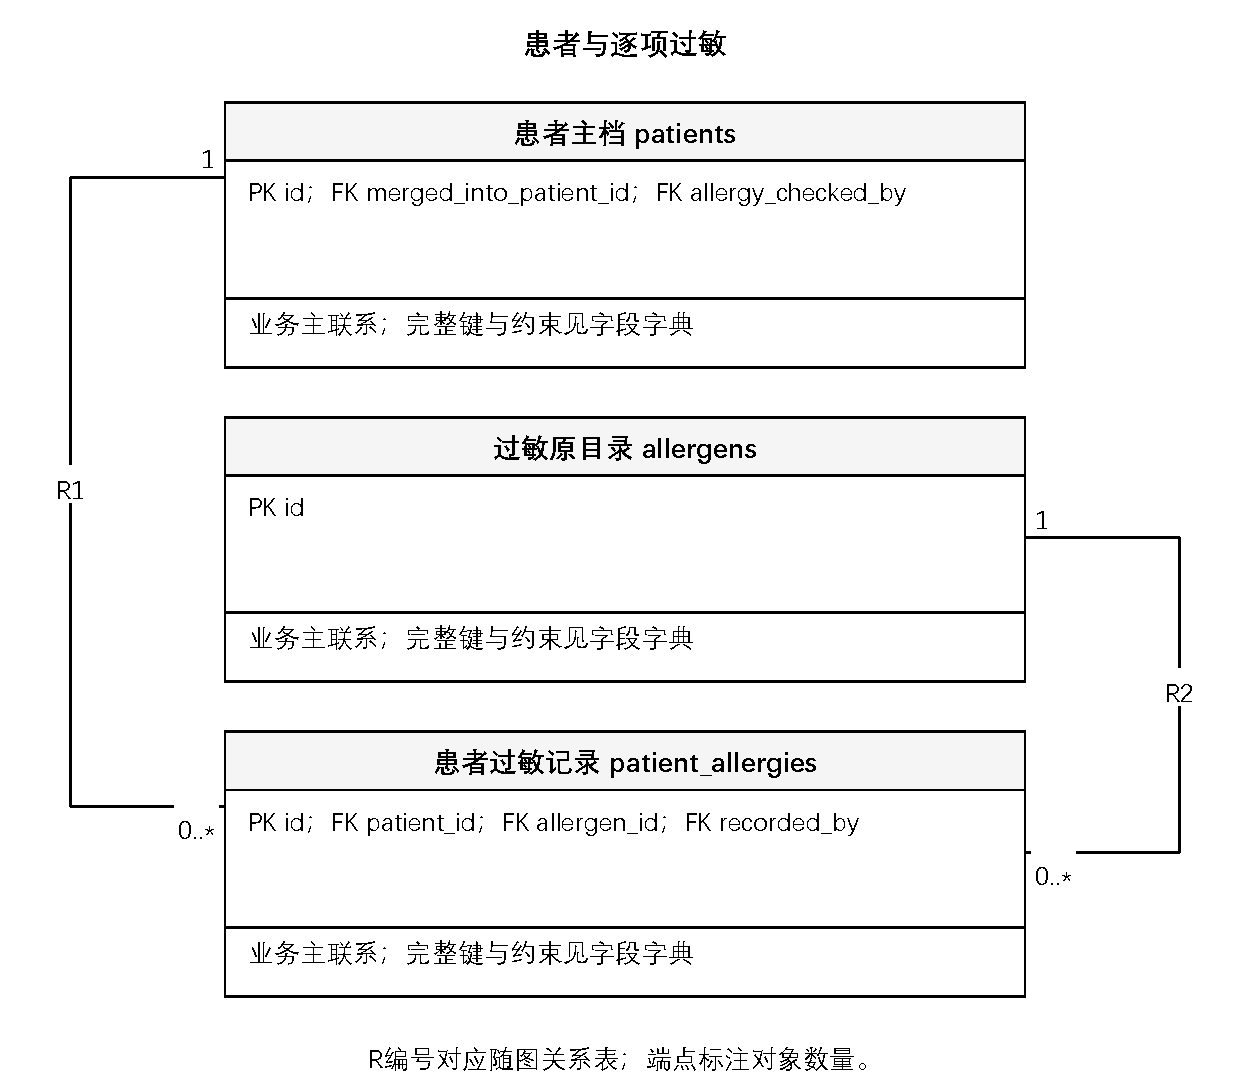
\includegraphics[width=\textwidth]{figures/er_concept_1.pdf}
\caption{患者与逐项过敏}\label{er_concept_1}\end{figure}
\par\noindent\begin{minipage}{\textwidth}
{\fontsize{10.5pt}{13.2pt}\selectfont\setlength{\tabcolsep}{0pt}\renewcommand{\arraystretch}{1.08}
\captionof{table}{患者与逐项过敏关联}\label{tab404}
\begin{tabular}{@{}p{1.240cm}@{\hspace{0.16cm}}p{10.040cm}@{\hspace{0.16cm}}p{3.840cm}@{}}
\toprule
\bfseries \Cell{编号} & \bfseries \Cell{外键联系} & \bfseries \Cell{父对象数/\allowbreak{}子对象数}\\\midrule
\Cell{R1} & \Cell{patients ← patient\_\allowbreak{}allergies.\allowbreak{}patient\_\allowbreak{}id} & \Cell{1 /\allowbreak{} 0.\allowbreak{}.\allowbreak{}*\allowbreak{}}\\[1pt]
\Cell{R2} & \Cell{allergens ← patient\_\allowbreak{}allergies.\allowbreak{}allergen\_\allowbreak{}id} & \Cell{1 /\allowbreak{} 0.\allowbreak{}.\allowbreak{}*\allowbreak{}}\\[1pt]
\bottomrule\end{tabular}
}\end{minipage}\par\vspace{6pt}
\begin{figure}[H]\centering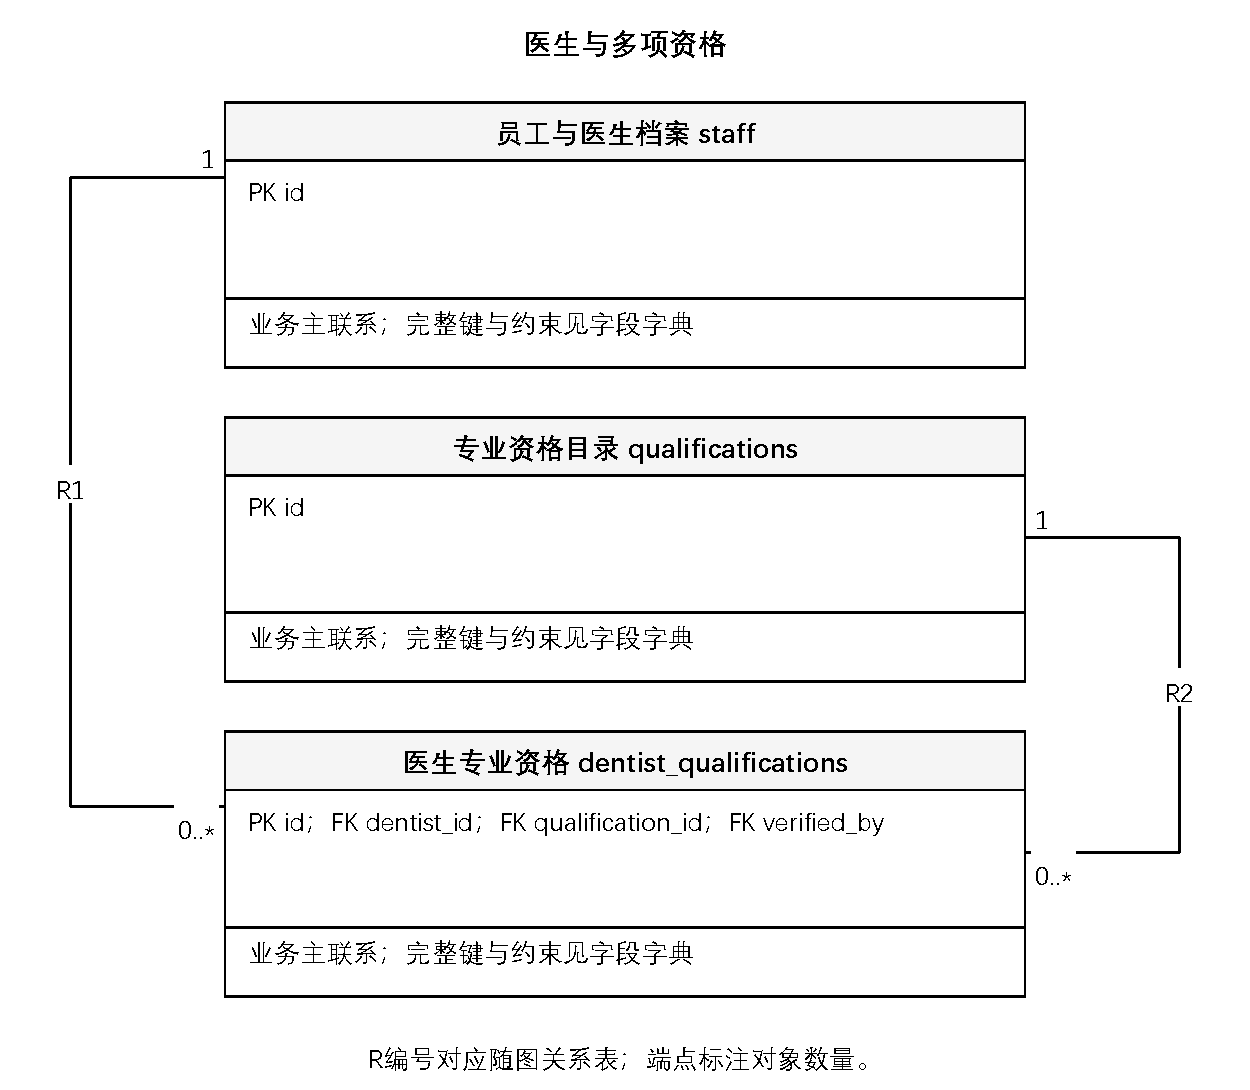
\includegraphics[width=\textwidth]{figures/er_concept_2.pdf}
\caption{医生与多项资格}\label{er_concept_2}\end{figure}
\par\noindent\begin{minipage}{\textwidth}
{\fontsize{10.5pt}{13.2pt}\selectfont\setlength{\tabcolsep}{0pt}\renewcommand{\arraystretch}{1.08}
\captionof{table}{医生与多项资格关联}\label{tab406}
\begin{tabular}{@{}p{1.240cm}@{\hspace{0.16cm}}p{10.040cm}@{\hspace{0.16cm}}p{3.840cm}@{}}
\toprule
\bfseries \Cell{编号} & \bfseries \Cell{外键联系} & \bfseries \Cell{父对象数/\allowbreak{}子对象数}\\\midrule
\Cell{R1} & \Cell{staff ← dentist\_\allowbreak{}qualifications.\allowbreak{}dentist\_\allowbreak{}id} & \Cell{1 /\allowbreak{} 0.\allowbreak{}.\allowbreak{}*\allowbreak{}}\\[1pt]
\Cell{R2} & \Cell{qualifications ← dentist\_\allowbreak{}qualifications.\allowbreak{}qualification\_\allowbreak{}id} & \Cell{1 /\allowbreak{} 0.\allowbreak{}.\allowbreak{}*\allowbreak{}}\\[1pt]
\bottomrule\end{tabular}
}\end{minipage}\par\vspace{6pt}
\begin{figure}[H]\centering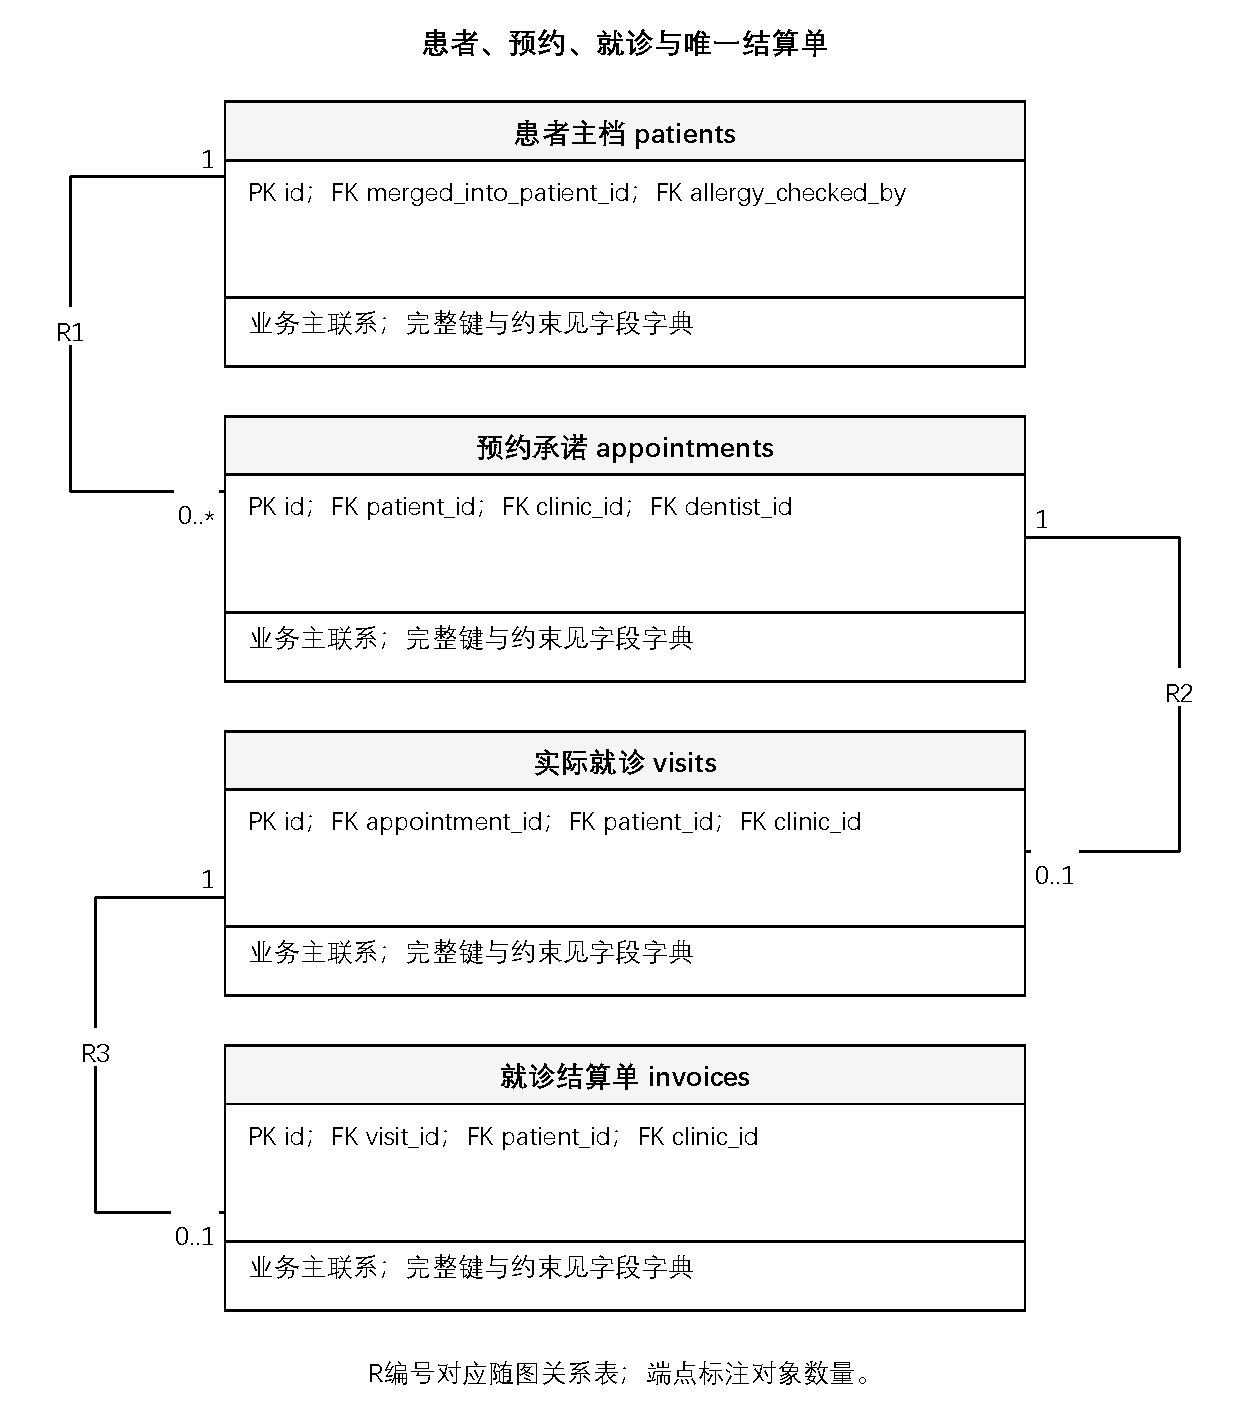
\includegraphics[width=\textwidth]{figures/er_concept_3.pdf}
\caption{患者、预约、就诊与唯一结算单}\label{er_concept_3}\end{figure}
\par\noindent\begin{minipage}{\textwidth}
{\fontsize{10.5pt}{13.2pt}\selectfont\setlength{\tabcolsep}{0pt}\renewcommand{\arraystretch}{1.08}
\captionof{table}{患者、预约、就诊与唯一结算单关联}\label{tab408}
\begin{tabular}{@{}p{1.240cm}@{\hspace{0.16cm}}p{10.040cm}@{\hspace{0.16cm}}p{3.840cm}@{}}
\toprule
\bfseries \Cell{编号} & \bfseries \Cell{外键联系} & \bfseries \Cell{父对象数/\allowbreak{}子对象数}\\\midrule
\Cell{R1} & \Cell{patients ← appointments.\allowbreak{}patient\_\allowbreak{}id} & \Cell{1 /\allowbreak{} 0.\allowbreak{}.\allowbreak{}*\allowbreak{}}\\[1pt]
\Cell{R2} & \Cell{appointments ← visits.\allowbreak{}appointment\_\allowbreak{}id} & \Cell{1 /\allowbreak{} 0.\allowbreak{}.\allowbreak{}1}\\[1pt]
\Cell{R3} & \Cell{visits ← invoices.\allowbreak{}visit\_\allowbreak{}id} & \Cell{1 /\allowbreak{} 0.\allowbreak{}.\allowbreak{}1}\\[1pt]
\bottomrule\end{tabular}
}\end{minipage}\par\vspace{6pt}
\begin{figure}[H]\centering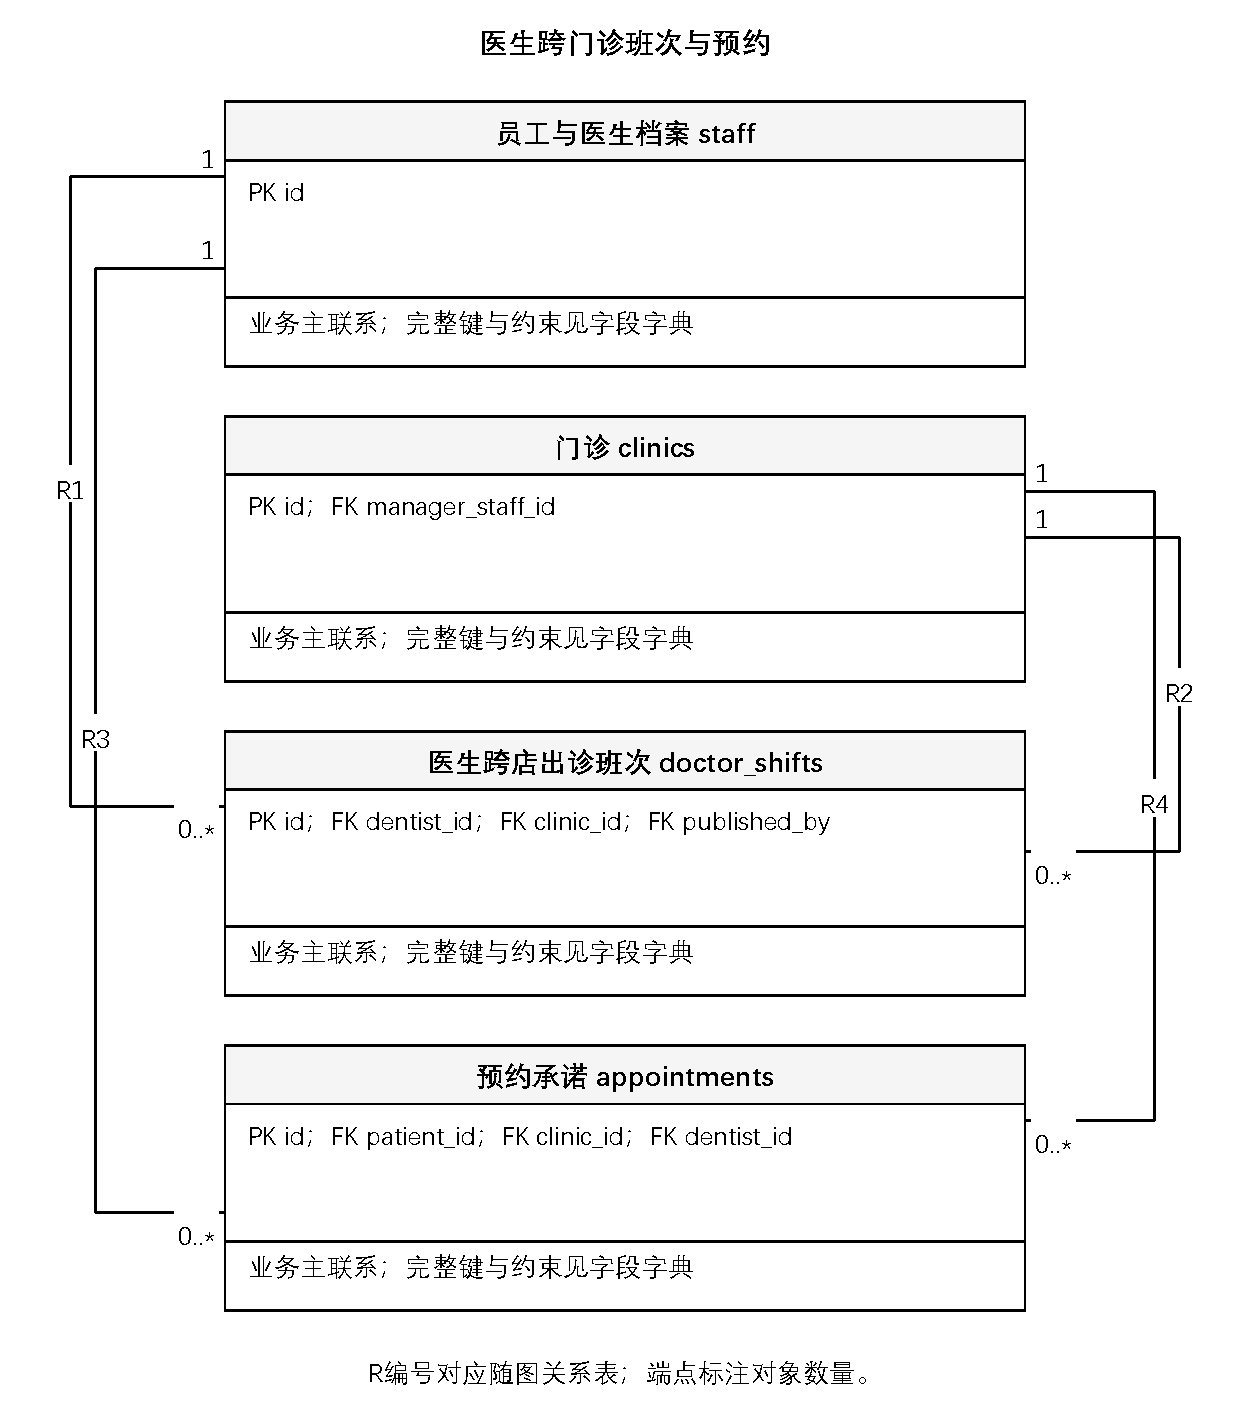
\includegraphics[width=\textwidth]{figures/er_concept_4.pdf}
\caption{医生跨门诊班次与预约}\label{er_concept_4}\end{figure}
\par\noindent\begin{minipage}{\textwidth}
{\fontsize{10.5pt}{13.2pt}\selectfont\setlength{\tabcolsep}{0pt}\renewcommand{\arraystretch}{1.08}
\captionof{table}{医生跨门诊班次与预约关联}\label{tab410}
\begin{tabular}{@{}p{1.240cm}@{\hspace{0.16cm}}p{10.040cm}@{\hspace{0.16cm}}p{3.840cm}@{}}
\toprule
\bfseries \Cell{编号} & \bfseries \Cell{外键联系} & \bfseries \Cell{父对象数/\allowbreak{}子对象数}\\\midrule
\Cell{R1} & \Cell{staff ← doctor\_\allowbreak{}shifts.\allowbreak{}dentist\_\allowbreak{}id} & \Cell{1 /\allowbreak{} 0.\allowbreak{}.\allowbreak{}*\allowbreak{}}\\[1pt]
\Cell{R2} & \Cell{clinics ← doctor\_\allowbreak{}shifts.\allowbreak{}clinic\_\allowbreak{}id} & \Cell{1 /\allowbreak{} 0.\allowbreak{}.\allowbreak{}*\allowbreak{}}\\[1pt]
\Cell{R3} & \Cell{staff ← appointments.\allowbreak{}dentist\_\allowbreak{}id} & \Cell{1 /\allowbreak{} 0.\allowbreak{}.\allowbreak{}*\allowbreak{}}\\[1pt]
\Cell{R4} & \Cell{clinics ← appointments.\allowbreak{}clinic\_\allowbreak{}id} & \Cell{1 /\allowbreak{} 0.\allowbreak{}.\allowbreak{}*\allowbreak{}}\\[1pt]
\bottomrule\end{tabular}
}\end{minipage}\par\vspace{6pt}
\begin{figure}[H]\centering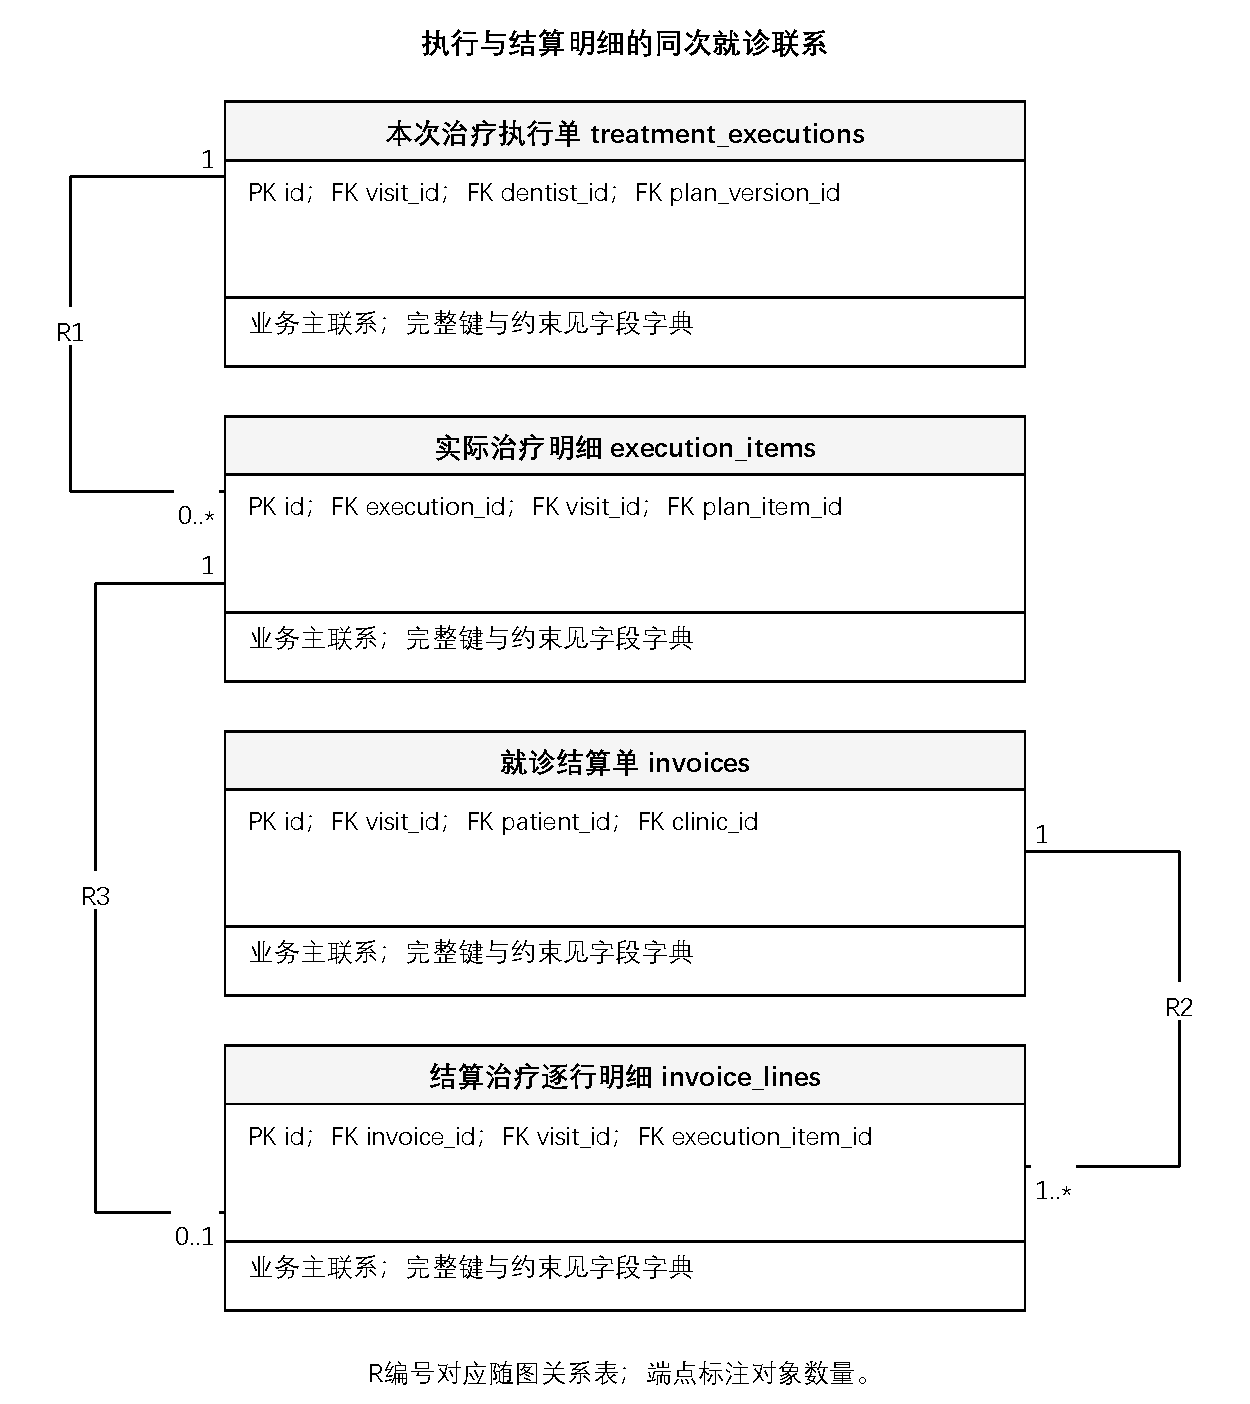
\includegraphics[width=\textwidth]{figures/er_concept_5.pdf}
\caption{执行与结算明细的同次就诊联系}\label{er_concept_5}\end{figure}
\par\noindent\begin{minipage}{\textwidth}
{\fontsize{10.5pt}{13.2pt}\selectfont\setlength{\tabcolsep}{0pt}\renewcommand{\arraystretch}{1.08}
\captionof{table}{执行与结算明细的同次就诊联系关联}\label{tab412}
\begin{tabular}{@{}p{1.240cm}@{\hspace{0.16cm}}p{10.040cm}@{\hspace{0.16cm}}p{3.840cm}@{}}
\toprule
\bfseries \Cell{编号} & \bfseries \Cell{外键联系} & \bfseries \Cell{父对象数/\allowbreak{}子对象数}\\\midrule
\Cell{R1} & \Cell{treatment\_\allowbreak{}executions ← execution\_\allowbreak{}items.\allowbreak{}execution\_\allowbreak{}id} & \Cell{1 /\allowbreak{} 0.\allowbreak{}.\allowbreak{}*\allowbreak{}}\\[1pt]
\Cell{R2} & \Cell{invoices ← invoice\_\allowbreak{}lines.\allowbreak{}invoice\_\allowbreak{}id} & \Cell{1 /\allowbreak{} 1.\allowbreak{}.\allowbreak{}*\allowbreak{}}\\[1pt]
\Cell{R3} & \Cell{execution\_\allowbreak{}items ← invoice\_\allowbreak{}lines.\allowbreak{}execution\_\allowbreak{}item\_\allowbreak{}id} & \Cell{1 /\allowbreak{} 0.\allowbreak{}.\allowbreak{}1}\\[1pt]
\bottomrule\end{tabular}
}\end{minipage}\par\vspace{6pt}
\begin{figure}[H]\centering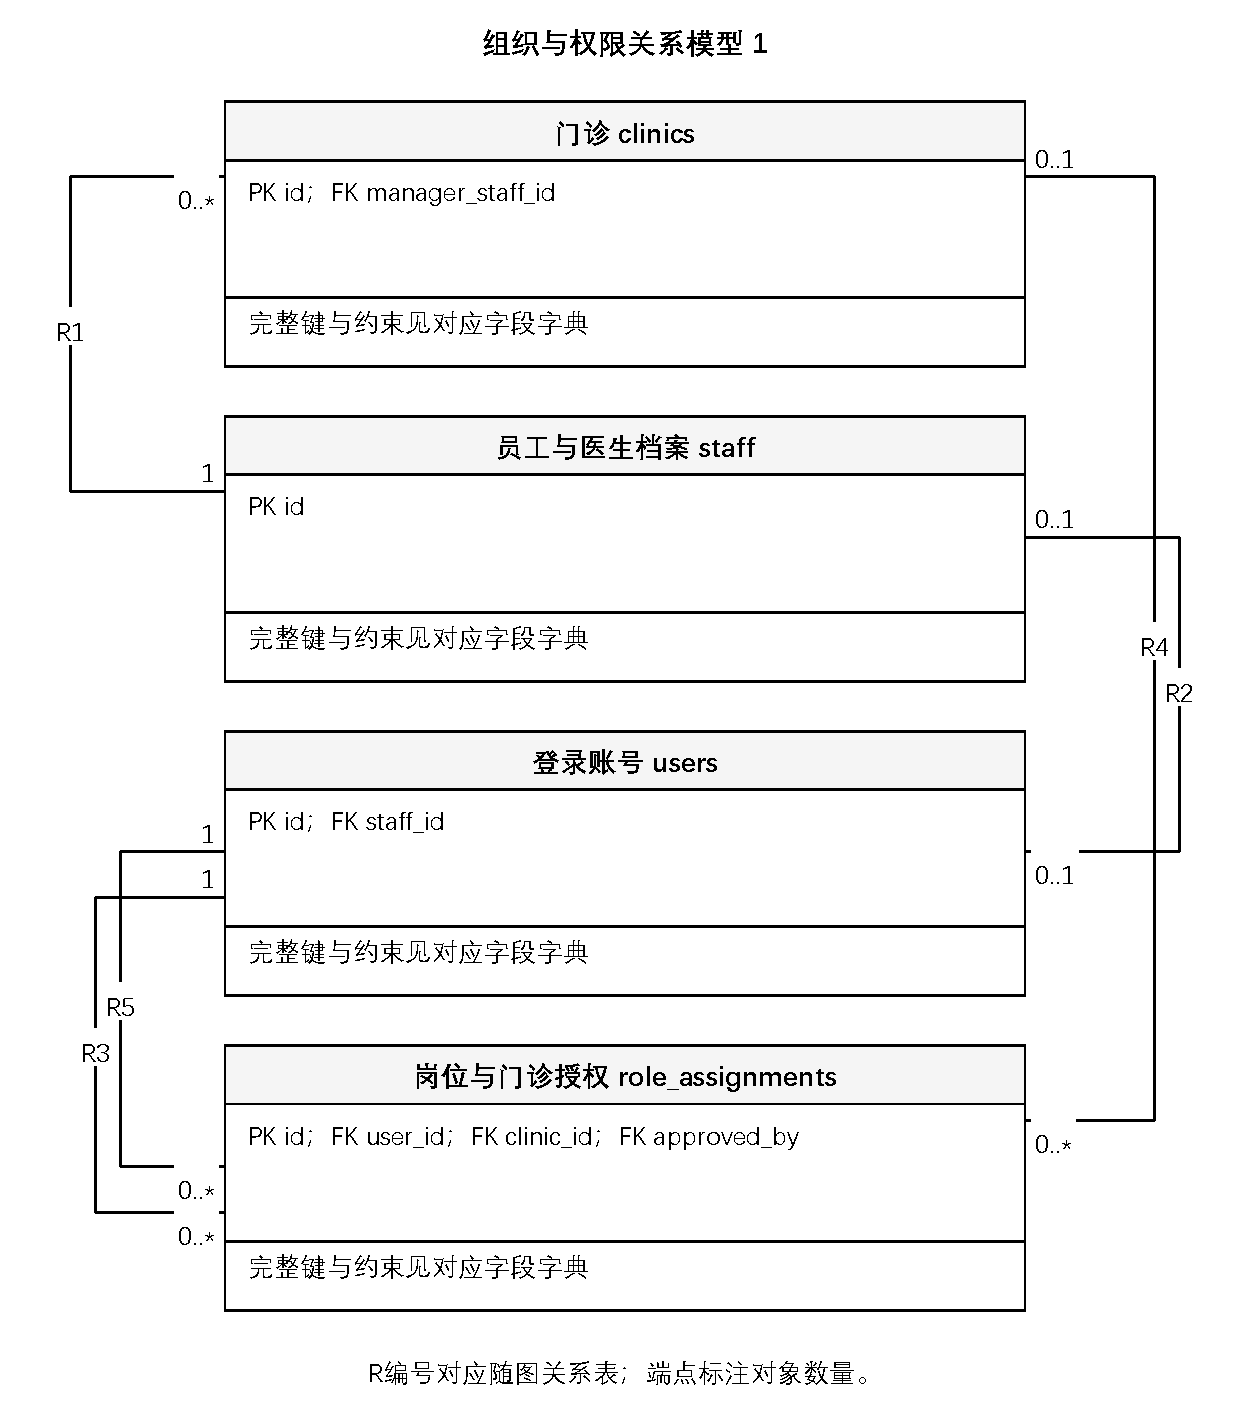
\includegraphics[width=\textwidth]{figures/er_6.pdf}
\caption{组织与权限关系模型 1}\label{er_6}\end{figure}
\par\noindent\begin{minipage}{\textwidth}
{\fontsize{10.5pt}{13.2pt}\selectfont\setlength{\tabcolsep}{0pt}\renewcommand{\arraystretch}{1.08}
\captionof{table}{组织与权限关系模型 1关联}\label{tab414}
\begin{tabular}{@{}p{1.240cm}@{\hspace{0.16cm}}p{10.040cm}@{\hspace{0.16cm}}p{3.840cm}@{}}
\toprule
\bfseries \Cell{编号} & \bfseries \Cell{外键联系} & \bfseries \Cell{父对象数/\allowbreak{}子对象数}\\\midrule
\Cell{R1} & \Cell{staff ← clinics.\allowbreak{}manager\_\allowbreak{}staff\_\allowbreak{}id} & \Cell{1 /\allowbreak{} 0.\allowbreak{}.\allowbreak{}*\allowbreak{}}\\[1pt]
\Cell{R2} & \Cell{staff ← users.\allowbreak{}staff\_\allowbreak{}id} & \Cell{0.\allowbreak{}.\allowbreak{}1 /\allowbreak{} 0.\allowbreak{}.\allowbreak{}1}\\[1pt]
\Cell{R3} & \Cell{users ← role\_\allowbreak{}assignments.\allowbreak{}user\_\allowbreak{}id} & \Cell{1 /\allowbreak{} 0.\allowbreak{}.\allowbreak{}*\allowbreak{}}\\[1pt]
\Cell{R4} & \Cell{clinics ← role\_\allowbreak{}assignments.\allowbreak{}clinic\_\allowbreak{}id} & \Cell{0.\allowbreak{}.\allowbreak{}1 /\allowbreak{} 0.\allowbreak{}.\allowbreak{}*\allowbreak{}}\\[1pt]
\Cell{R5} & \Cell{users ← role\_\allowbreak{}assignments.\allowbreak{}approved\_\allowbreak{}by} & \Cell{1 /\allowbreak{} 0.\allowbreak{}.\allowbreak{}*\allowbreak{}}\\[1pt]
\bottomrule\end{tabular}
}\end{minipage}\par\vspace{6pt}
\begin{figure}[H]\centering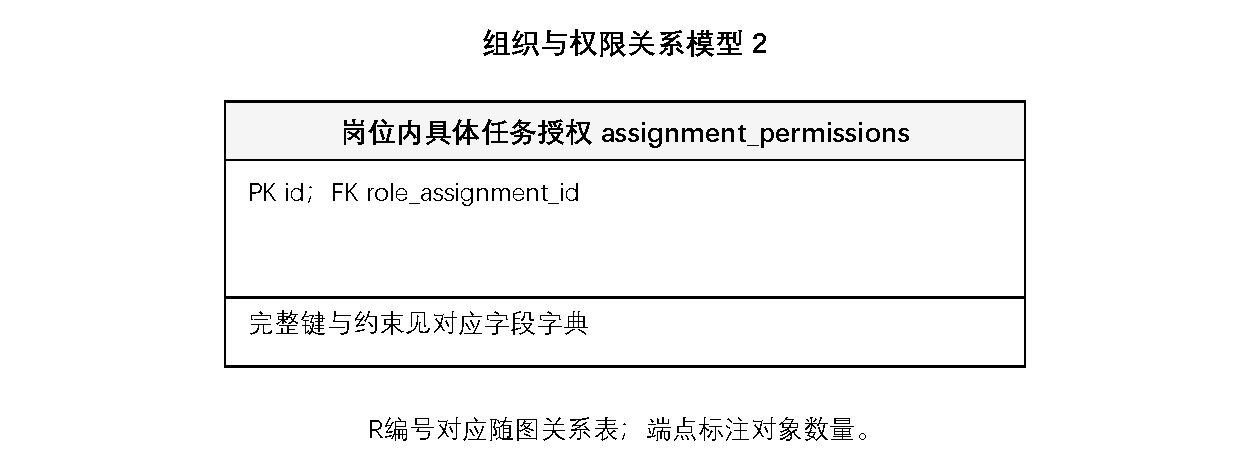
\includegraphics[width=\textwidth]{figures/er_7.pdf}
\caption{组织与权限关系模型 2}\label{er_7}\end{figure}
\begin{figure}[H]\centering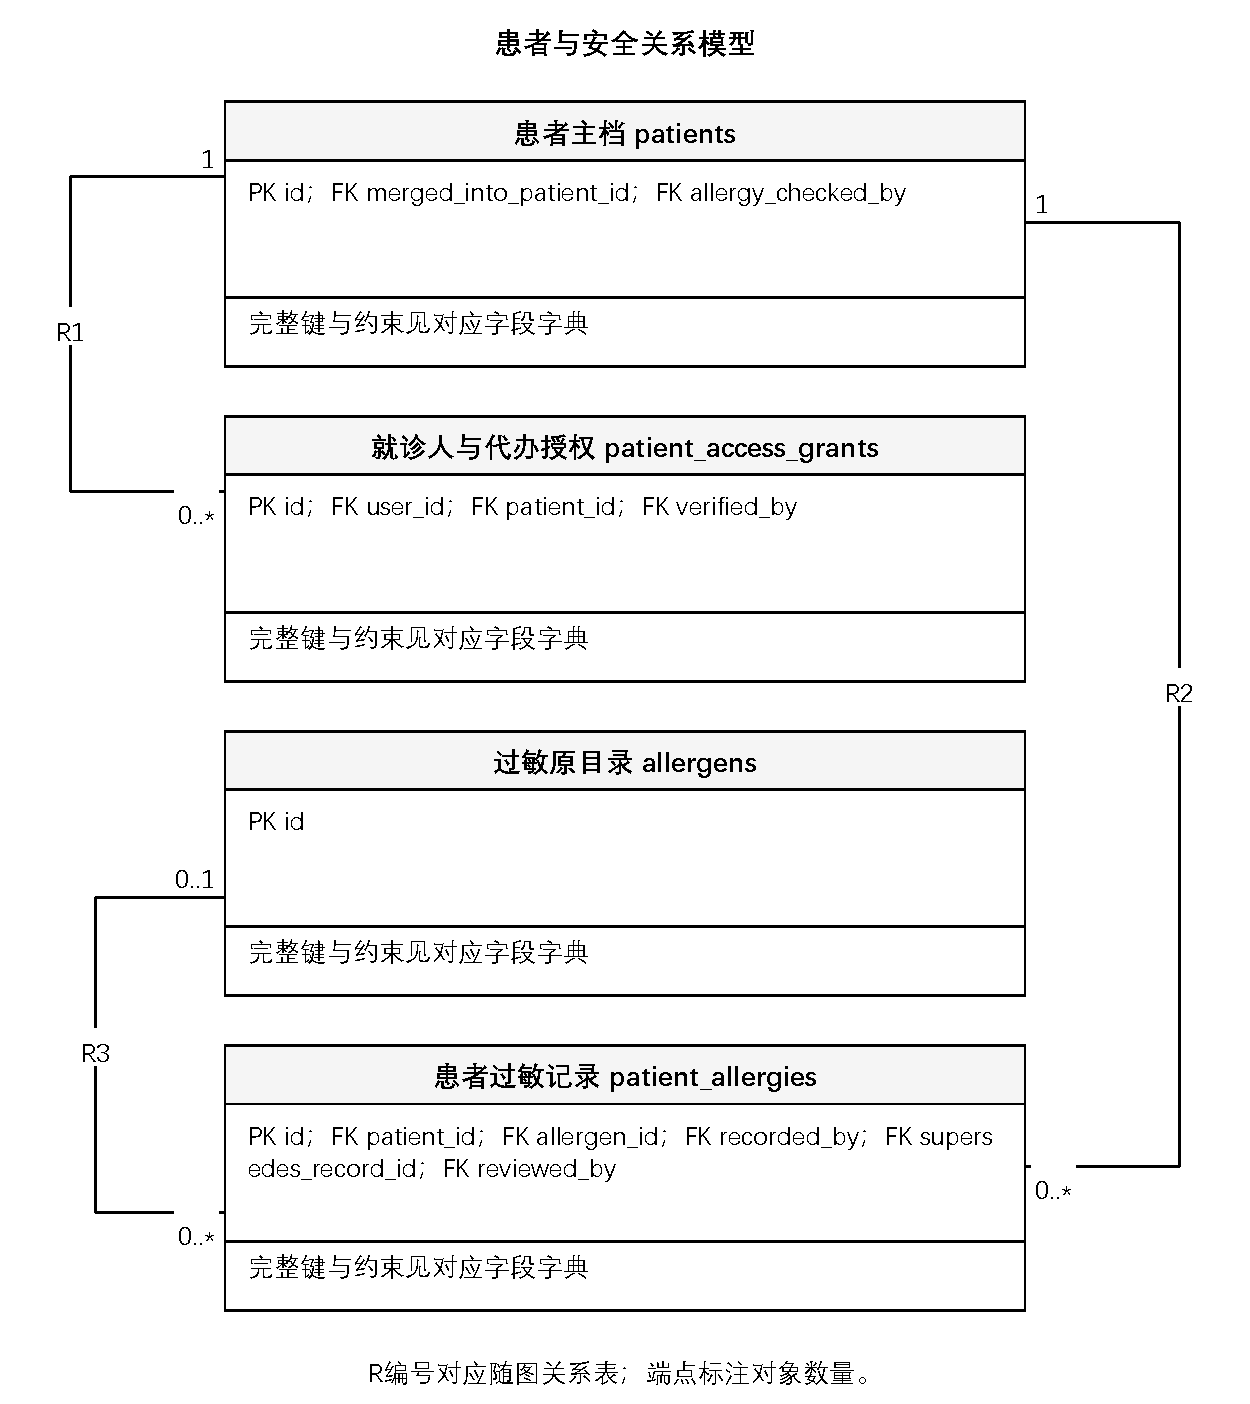
\includegraphics[width=\textwidth]{figures/er_8.pdf}
\caption{患者与安全关系模型}\label{er_8}\end{figure}
\par\noindent\begin{minipage}{\textwidth}
{\fontsize{10.5pt}{13.2pt}\selectfont\setlength{\tabcolsep}{0pt}\renewcommand{\arraystretch}{1.08}
\captionof{table}{患者与安全关系模型关联}\label{tab417}
\begin{tabular}{@{}p{1.240cm}@{\hspace{0.16cm}}p{10.040cm}@{\hspace{0.16cm}}p{3.840cm}@{}}
\toprule
\bfseries \Cell{编号} & \bfseries \Cell{外键联系} & \bfseries \Cell{父对象数/\allowbreak{}子对象数}\\\midrule
\Cell{R1} & \Cell{patients ← patient\_\allowbreak{}access\_\allowbreak{}grants.\allowbreak{}patient\_\allowbreak{}id} & \Cell{1 /\allowbreak{} 0.\allowbreak{}.\allowbreak{}*\allowbreak{}}\\[1pt]
\Cell{R2} & \Cell{patients ← patient\_\allowbreak{}allergies.\allowbreak{}patient\_\allowbreak{}id} & \Cell{1 /\allowbreak{} 0.\allowbreak{}.\allowbreak{}*\allowbreak{}}\\[1pt]
\Cell{R3} & \Cell{allergens ← patient\_\allowbreak{}allergies.\allowbreak{}allergen\_\allowbreak{}id} & \Cell{0.\allowbreak{}.\allowbreak{}1 /\allowbreak{} 0.\allowbreak{}.\allowbreak{}*\allowbreak{}}\\[1pt]
\bottomrule\end{tabular}
}\end{minipage}\par\vspace{6pt}
\begin{figure}[H]\centering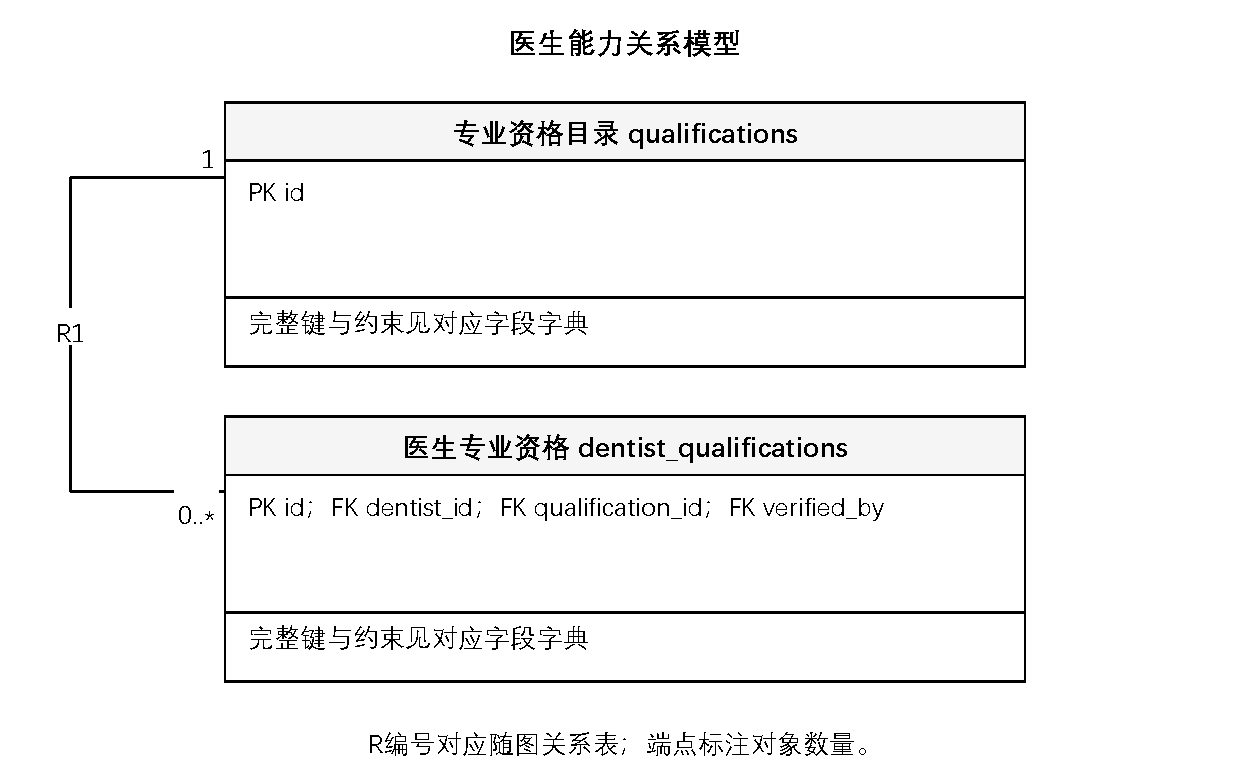
\includegraphics[width=\textwidth]{figures/er_9.pdf}
\caption{医生能力关系模型}\label{er_9}\end{figure}
\par\noindent\begin{minipage}{\textwidth}
{\fontsize{10.5pt}{13.2pt}\selectfont\setlength{\tabcolsep}{0pt}\renewcommand{\arraystretch}{1.08}
\captionof{table}{医生能力关系模型关联}\label{tab419}
\begin{tabular}{@{}p{1.240cm}@{\hspace{0.16cm}}p{10.040cm}@{\hspace{0.16cm}}p{3.840cm}@{}}
\toprule
\bfseries \Cell{编号} & \bfseries \Cell{外键联系} & \bfseries \Cell{父对象数/\allowbreak{}子对象数}\\\midrule
\Cell{R1} & \Cell{qualifications ← dentist\_\allowbreak{}qualifications.\allowbreak{}qualification\_\allowbreak{}id} & \Cell{1 /\allowbreak{} 0.\allowbreak{}.\allowbreak{}*\allowbreak{}}\\[1pt]
\bottomrule\end{tabular}
}\end{minipage}\par\vspace{6pt}
\begin{figure}[H]\centering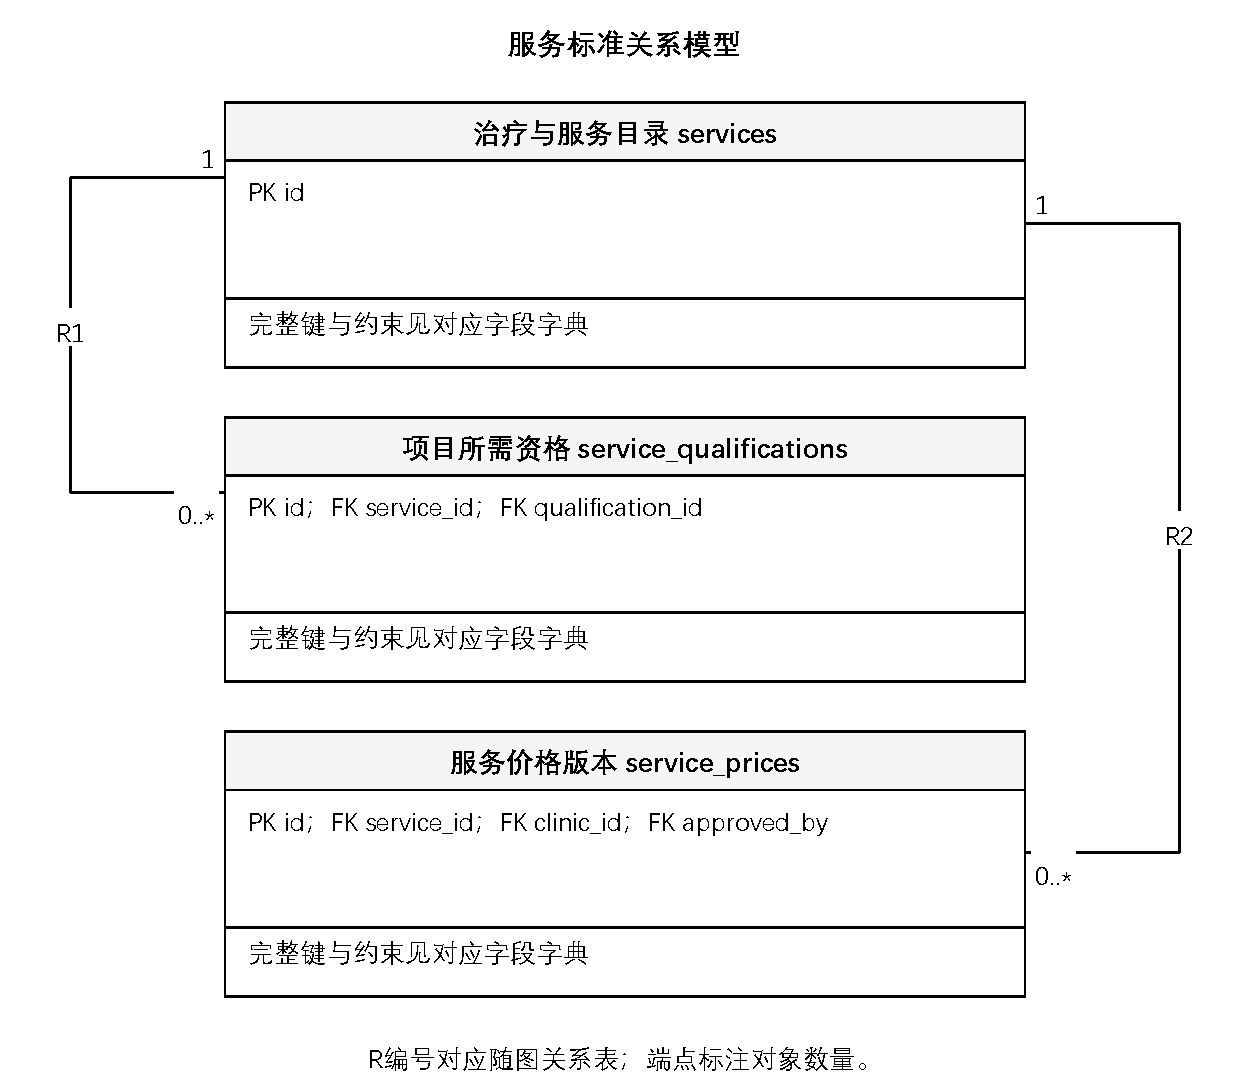
\includegraphics[width=\textwidth]{figures/er_10.pdf}
\caption{服务标准关系模型}\label{er_10}\end{figure}
\par\noindent\begin{minipage}{\textwidth}
{\fontsize{10.5pt}{13.2pt}\selectfont\setlength{\tabcolsep}{0pt}\renewcommand{\arraystretch}{1.08}
\captionof{table}{服务标准关系模型关联}\label{tab421}
\begin{tabular}{@{}p{1.240cm}@{\hspace{0.16cm}}p{10.040cm}@{\hspace{0.16cm}}p{3.840cm}@{}}
\toprule
\bfseries \Cell{编号} & \bfseries \Cell{外键联系} & \bfseries \Cell{父对象数/\allowbreak{}子对象数}\\\midrule
\Cell{R1} & \Cell{services ← service\_\allowbreak{}qualifications.\allowbreak{}service\_\allowbreak{}id} & \Cell{1 /\allowbreak{} 0.\allowbreak{}.\allowbreak{}*\allowbreak{}}\\[1pt]
\Cell{R2} & \Cell{services ← service\_\allowbreak{}prices.\allowbreak{}service\_\allowbreak{}id} & \Cell{1 /\allowbreak{} 0.\allowbreak{}.\allowbreak{}*\allowbreak{}}\\[1pt]
\bottomrule\end{tabular}
}\end{minipage}\par\vspace{6pt}
\begin{figure}[H]\centering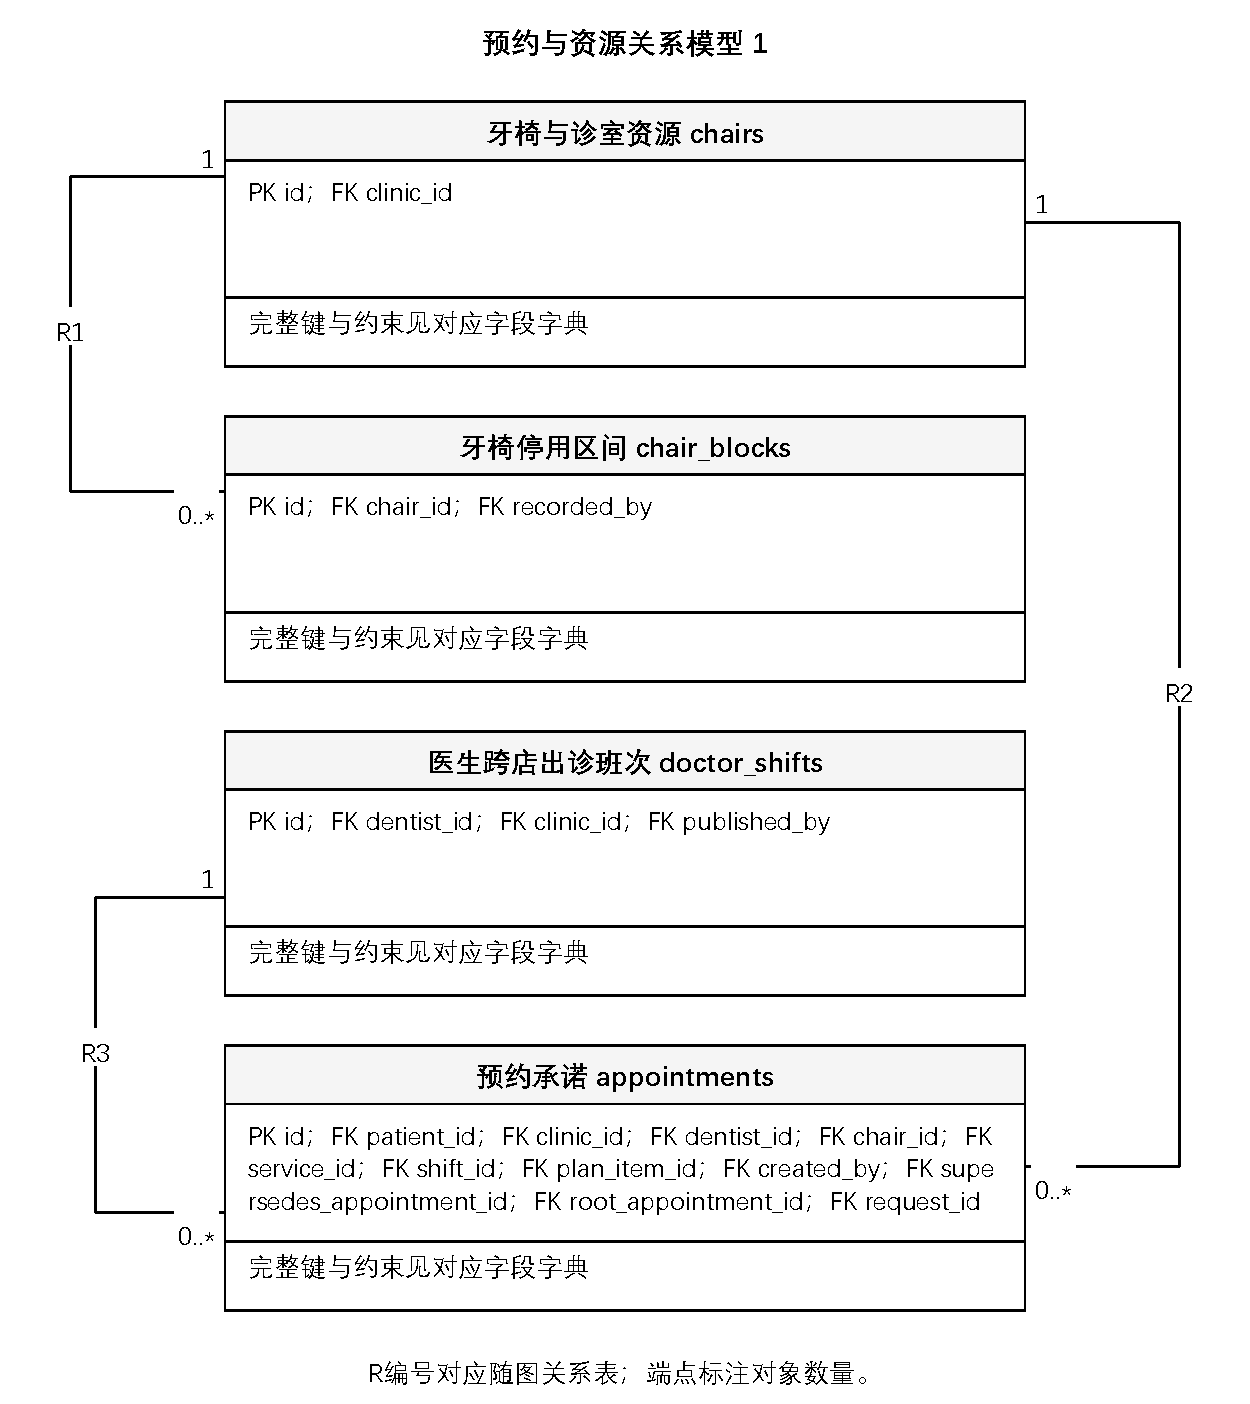
\includegraphics[width=\textwidth]{figures/er_11.pdf}
\caption{预约与资源关系模型 1}\label{er_11}\end{figure}
\par\noindent\begin{minipage}{\textwidth}
{\fontsize{10.5pt}{13.2pt}\selectfont\setlength{\tabcolsep}{0pt}\renewcommand{\arraystretch}{1.08}
\captionof{table}{预约与资源关系模型 1关联}\label{tab423}
\begin{tabular}{@{}p{1.240cm}@{\hspace{0.16cm}}p{10.040cm}@{\hspace{0.16cm}}p{3.840cm}@{}}
\toprule
\bfseries \Cell{编号} & \bfseries \Cell{外键联系} & \bfseries \Cell{父对象数/\allowbreak{}子对象数}\\\midrule
\Cell{R1} & \Cell{chairs ← chair\_\allowbreak{}blocks.\allowbreak{}chair\_\allowbreak{}id} & \Cell{1 /\allowbreak{} 0.\allowbreak{}.\allowbreak{}*\allowbreak{}}\\[1pt]
\Cell{R2} & \Cell{chairs ← appointments.\allowbreak{}chair\_\allowbreak{}id} & \Cell{1 /\allowbreak{} 0.\allowbreak{}.\allowbreak{}*\allowbreak{}}\\[1pt]
\Cell{R3} & \Cell{doctor\_\allowbreak{}shifts ← appointments.\allowbreak{}shift\_\allowbreak{}id} & \Cell{1 /\allowbreak{} 0.\allowbreak{}.\allowbreak{}*\allowbreak{}}\\[1pt]
\bottomrule\end{tabular}
}\end{minipage}\par\vspace{6pt}
\begin{figure}[H]\centering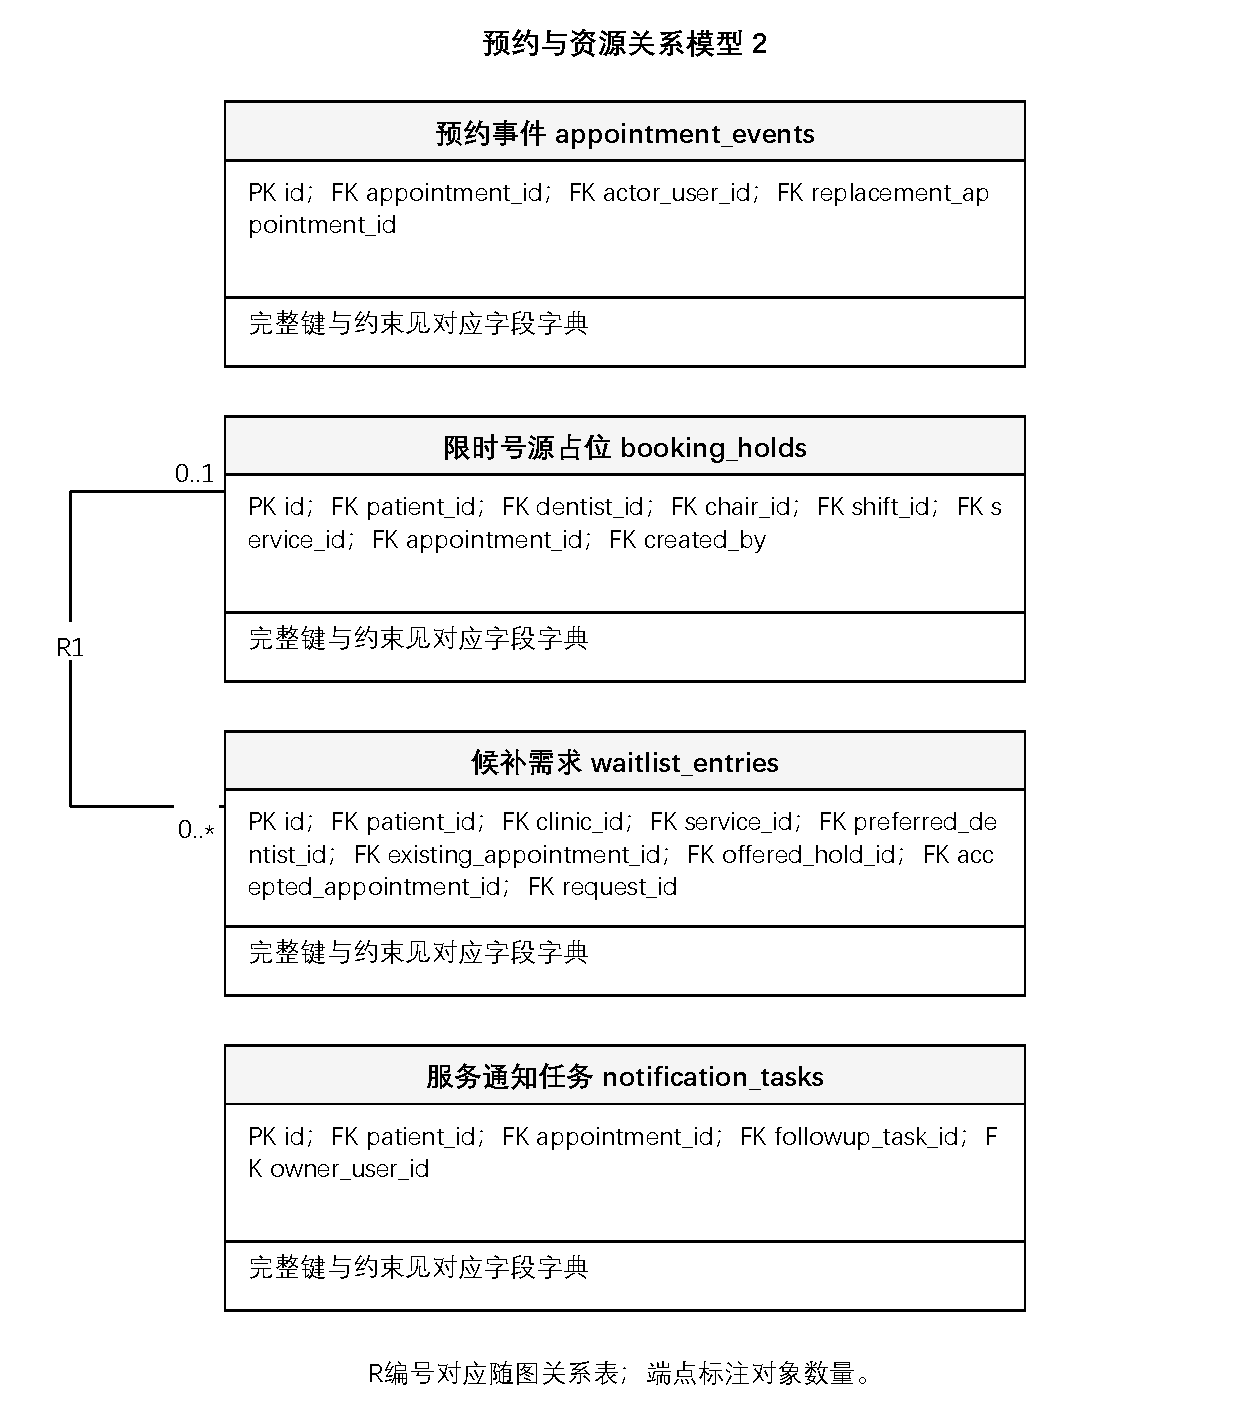
\includegraphics[width=\textwidth]{figures/er_12.pdf}
\caption{预约与资源关系模型 2}\label{er_12}\end{figure}
\par\noindent\begin{minipage}{\textwidth}
{\fontsize{10.5pt}{13.2pt}\selectfont\setlength{\tabcolsep}{0pt}\renewcommand{\arraystretch}{1.08}
\captionof{table}{预约与资源关系模型 2关联}\label{tab425}
\begin{tabular}{@{}p{1.240cm}@{\hspace{0.16cm}}p{10.040cm}@{\hspace{0.16cm}}p{3.840cm}@{}}
\toprule
\bfseries \Cell{编号} & \bfseries \Cell{外键联系} & \bfseries \Cell{父对象数/\allowbreak{}子对象数}\\\midrule
\Cell{R1} & \Cell{booking\_\allowbreak{}holds ← waitlist\_\allowbreak{}entries.\allowbreak{}offered\_\allowbreak{}hold\_\allowbreak{}id} & \Cell{0.\allowbreak{}.\allowbreak{}1 /\allowbreak{} 0.\allowbreak{}.\allowbreak{}*\allowbreak{}}\\[1pt]
\bottomrule\end{tabular}
}\end{minipage}\par\vspace{6pt}
\begin{figure}[H]\centering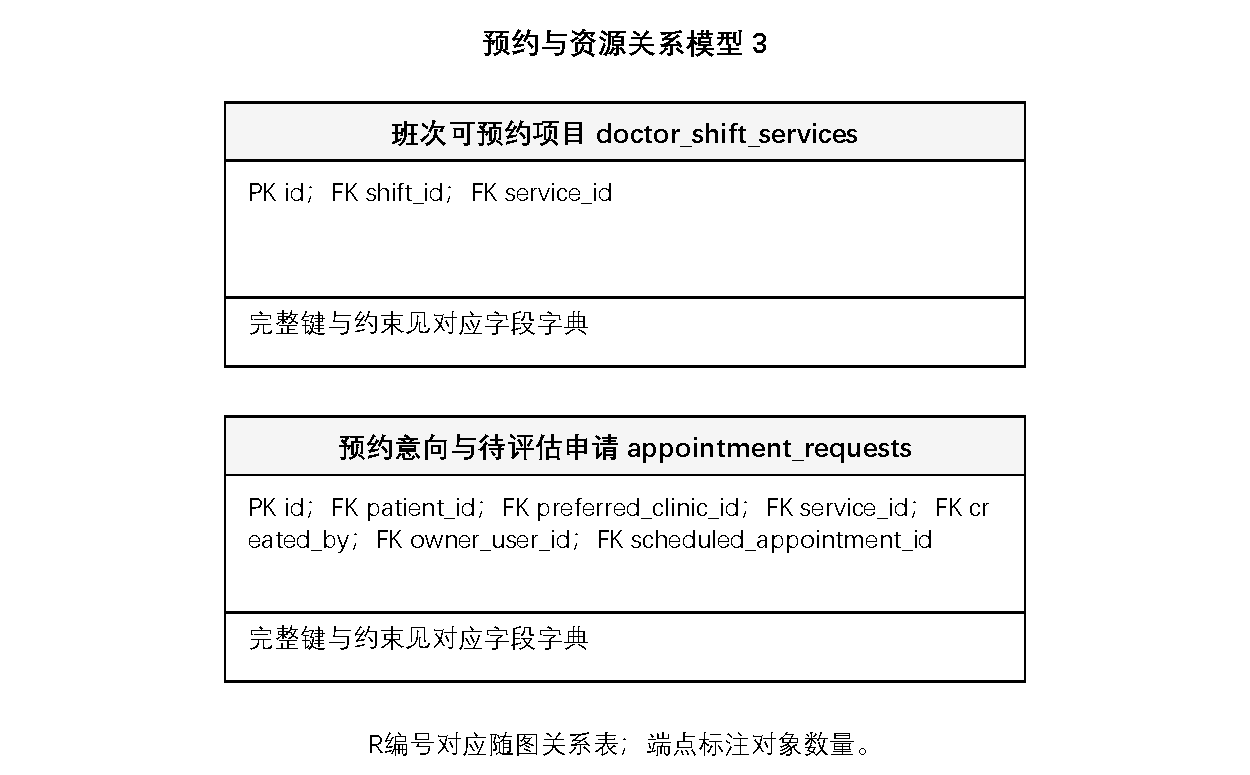
\includegraphics[width=\textwidth]{figures/er_13.pdf}
\caption{预约与资源关系模型 3}\label{er_13}\end{figure}
\begin{figure}[H]\centering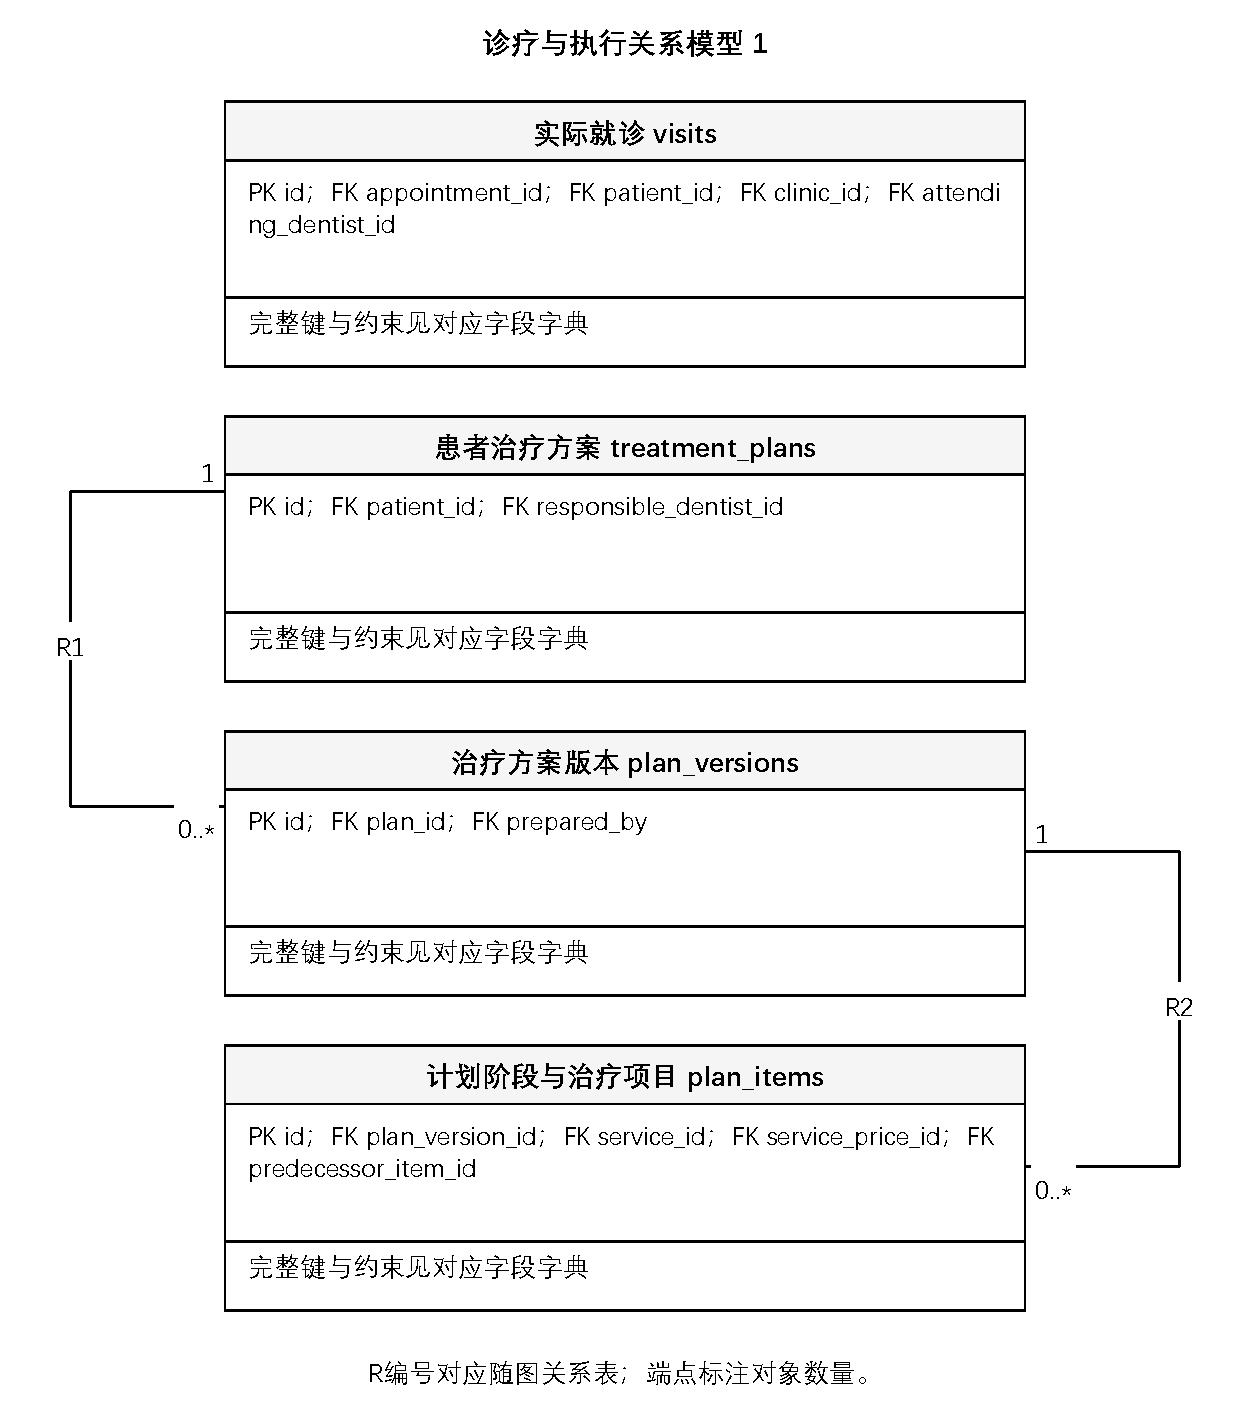
\includegraphics[width=\textwidth]{figures/er_14.pdf}
\caption{诊疗与执行关系模型 1}\label{er_14}\end{figure}
\par\noindent\begin{minipage}{\textwidth}
{\fontsize{10.5pt}{13.2pt}\selectfont\setlength{\tabcolsep}{0pt}\renewcommand{\arraystretch}{1.08}
\captionof{table}{诊疗与执行关系模型 1关联}\label{tab428}
\begin{tabular}{@{}p{1.240cm}@{\hspace{0.16cm}}p{10.040cm}@{\hspace{0.16cm}}p{3.840cm}@{}}
\toprule
\bfseries \Cell{编号} & \bfseries \Cell{外键联系} & \bfseries \Cell{父对象数/\allowbreak{}子对象数}\\\midrule
\Cell{R1} & \Cell{treatment\_\allowbreak{}plans ← plan\_\allowbreak{}versions.\allowbreak{}plan\_\allowbreak{}id} & \Cell{1 /\allowbreak{} 0.\allowbreak{}.\allowbreak{}*\allowbreak{}}\\[1pt]
\Cell{R2} & \Cell{plan\_\allowbreak{}versions ← plan\_\allowbreak{}items.\allowbreak{}plan\_\allowbreak{}version\_\allowbreak{}id} & \Cell{1 /\allowbreak{} 0.\allowbreak{}.\allowbreak{}*\allowbreak{}}\\[1pt]
\bottomrule\end{tabular}
}\end{minipage}\par\vspace{6pt}
\begin{figure}[H]\centering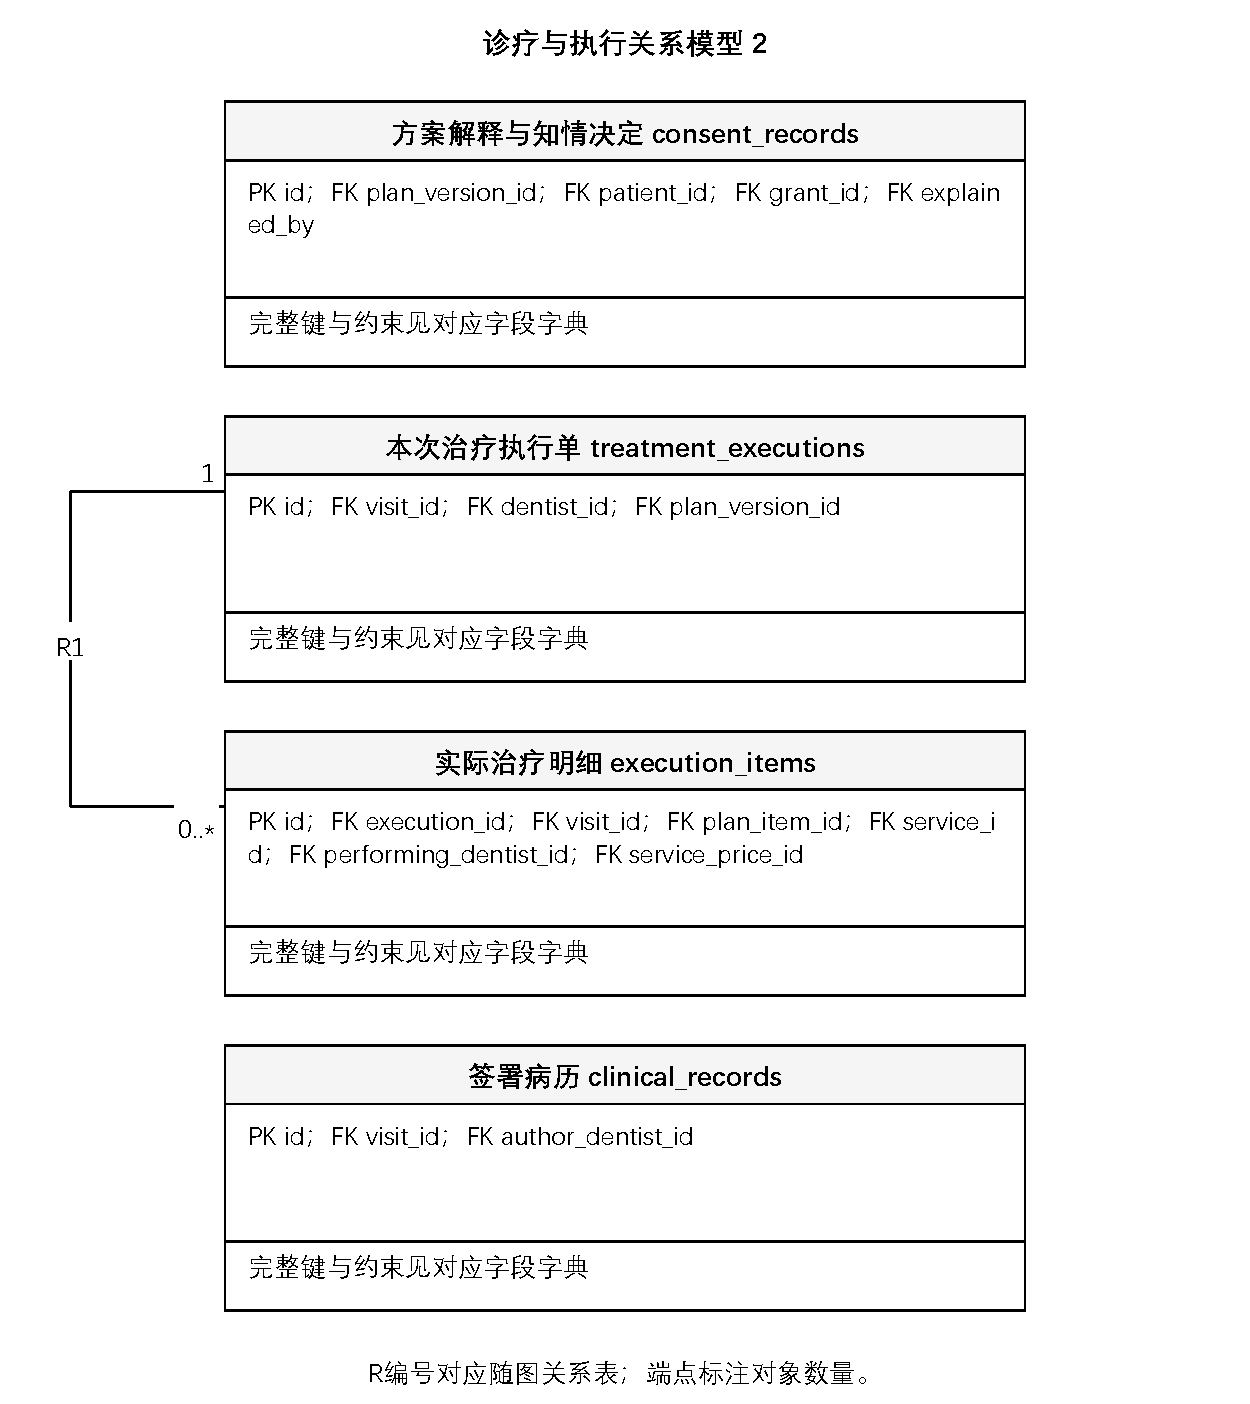
\includegraphics[width=\textwidth]{figures/er_15.pdf}
\caption{诊疗与执行关系模型 2}\label{er_15}\end{figure}
\par\noindent\begin{minipage}{\textwidth}
{\fontsize{10.5pt}{13.2pt}\selectfont\setlength{\tabcolsep}{0pt}\renewcommand{\arraystretch}{1.08}
\captionof{table}{诊疗与执行关系模型 2关联}\label{tab430}
\begin{tabular}{@{}p{1.240cm}@{\hspace{0.16cm}}p{10.040cm}@{\hspace{0.16cm}}p{3.840cm}@{}}
\toprule
\bfseries \Cell{编号} & \bfseries \Cell{外键联系} & \bfseries \Cell{父对象数/\allowbreak{}子对象数}\\\midrule
\Cell{R1} & \Cell{treatment\_\allowbreak{}executions ← execution\_\allowbreak{}items.\allowbreak{}execution\_\allowbreak{}id} & \Cell{1 /\allowbreak{} 0.\allowbreak{}.\allowbreak{}*\allowbreak{}}\\[1pt]
\bottomrule\end{tabular}
}\end{minipage}\par\vspace{6pt}
\begin{figure}[H]\centering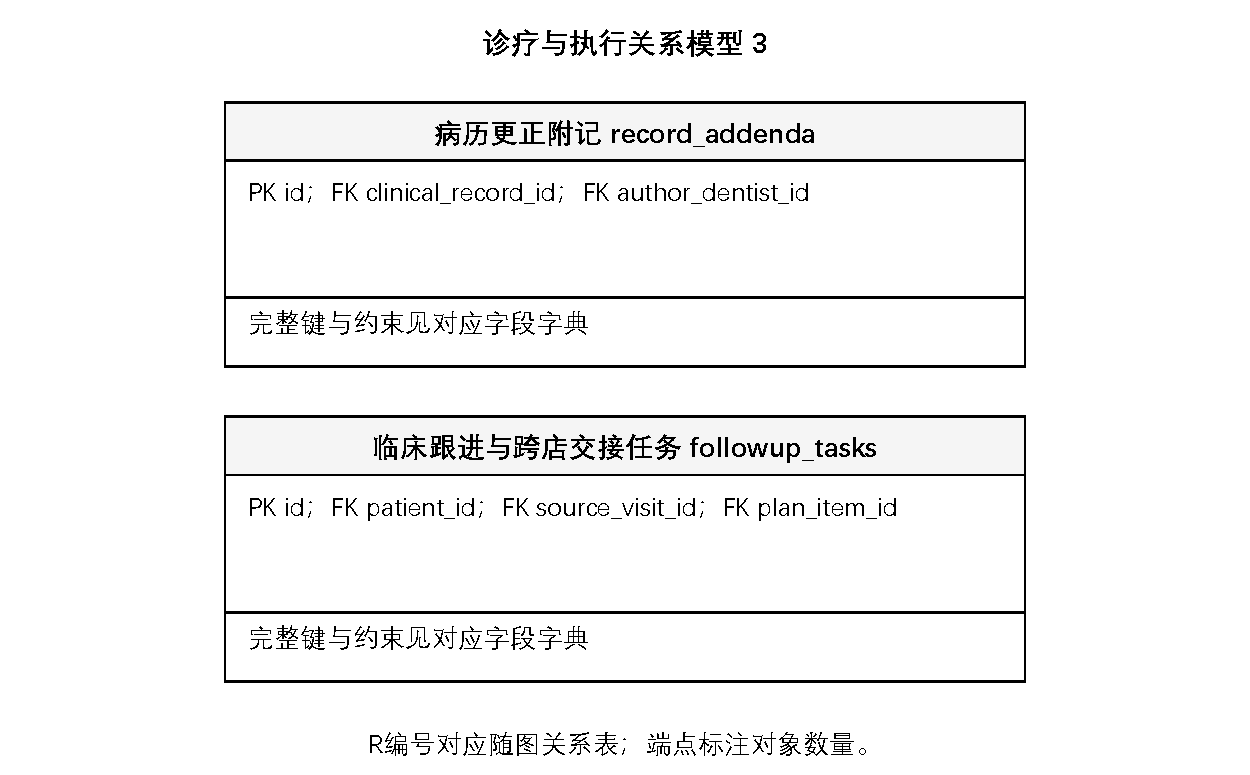
\includegraphics[width=\textwidth]{figures/er_16.pdf}
\caption{诊疗与执行关系模型 3}\label{er_16}\end{figure}
\begin{figure}[H]\centering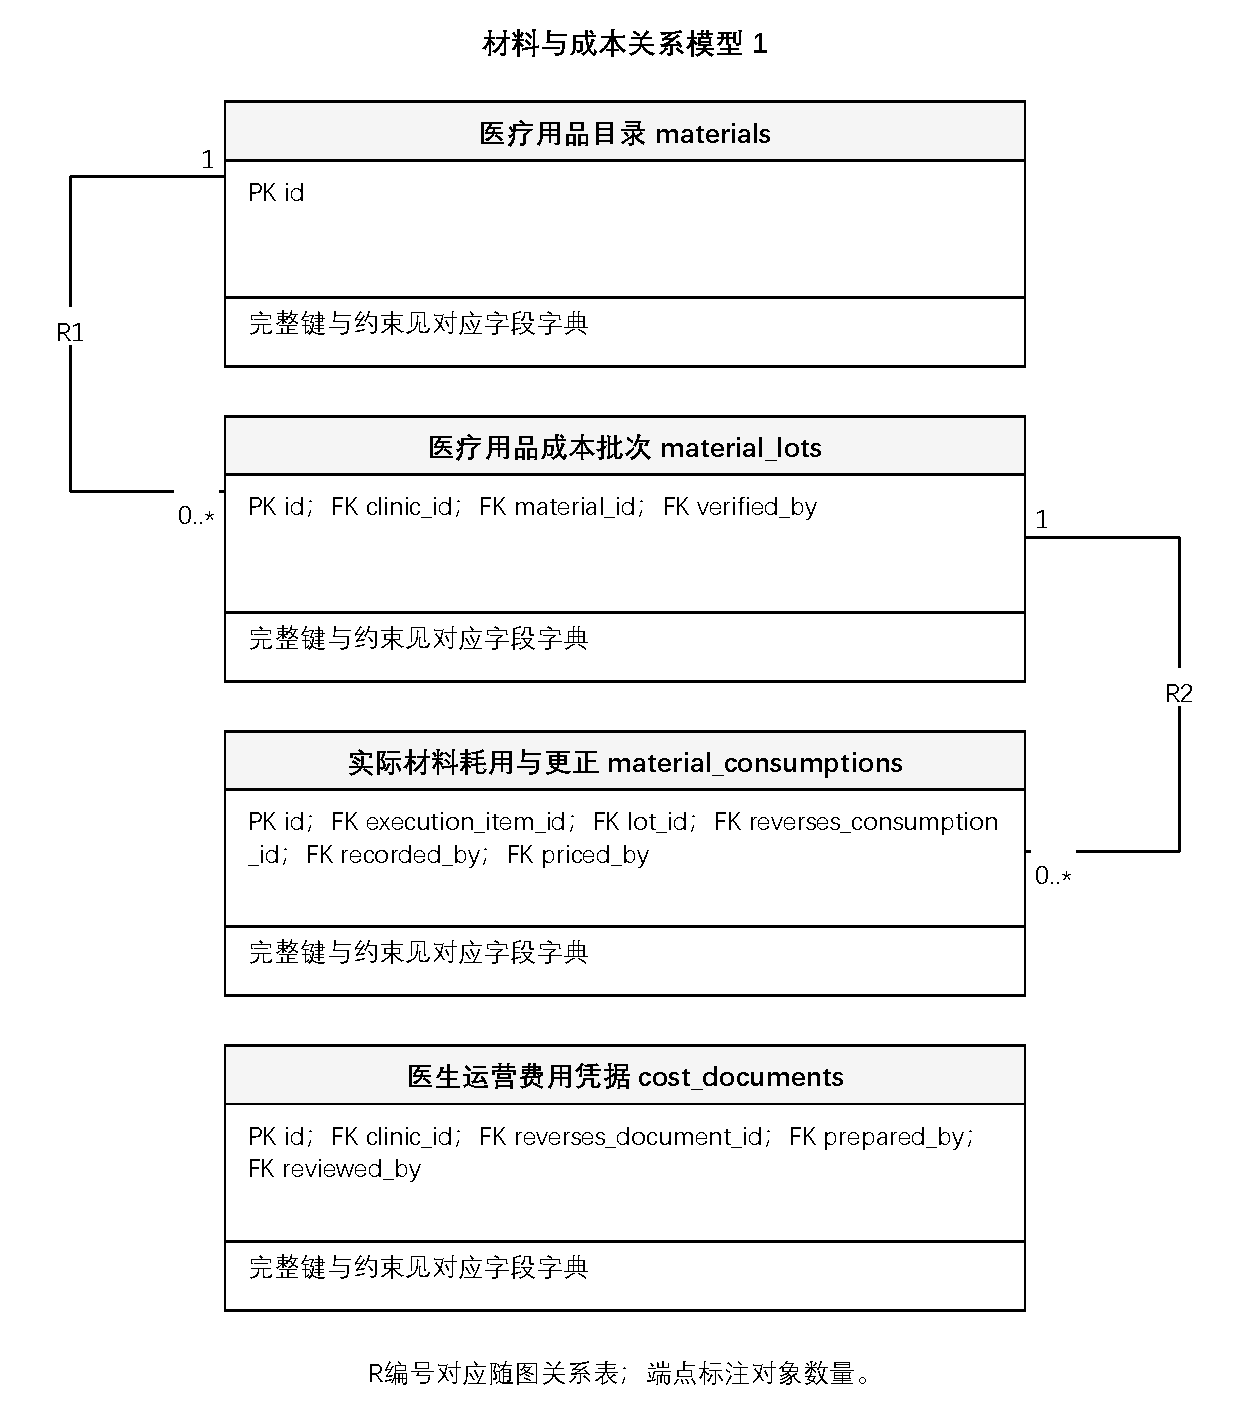
\includegraphics[width=\textwidth]{figures/er_17.pdf}
\caption{材料与成本关系模型 1}\label{er_17}\end{figure}
\par\noindent\begin{minipage}{\textwidth}
{\fontsize{10.5pt}{13.2pt}\selectfont\setlength{\tabcolsep}{0pt}\renewcommand{\arraystretch}{1.08}
\captionof{table}{材料与成本关系模型 1关联}\label{tab433}
\begin{tabular}{@{}p{1.240cm}@{\hspace{0.16cm}}p{10.040cm}@{\hspace{0.16cm}}p{3.840cm}@{}}
\toprule
\bfseries \Cell{编号} & \bfseries \Cell{外键联系} & \bfseries \Cell{父对象数/\allowbreak{}子对象数}\\\midrule
\Cell{R1} & \Cell{materials ← material\_\allowbreak{}lots.\allowbreak{}material\_\allowbreak{}id} & \Cell{1 /\allowbreak{} 0.\allowbreak{}.\allowbreak{}*\allowbreak{}}\\[1pt]
\Cell{R2} & \Cell{material\_\allowbreak{}lots ← material\_\allowbreak{}consumptions.\allowbreak{}lot\_\allowbreak{}id} & \Cell{1 /\allowbreak{} 0.\allowbreak{}.\allowbreak{}*\allowbreak{}}\\[1pt]
\bottomrule\end{tabular}
}\end{minipage}\par\vspace{6pt}
\begin{figure}[H]\centering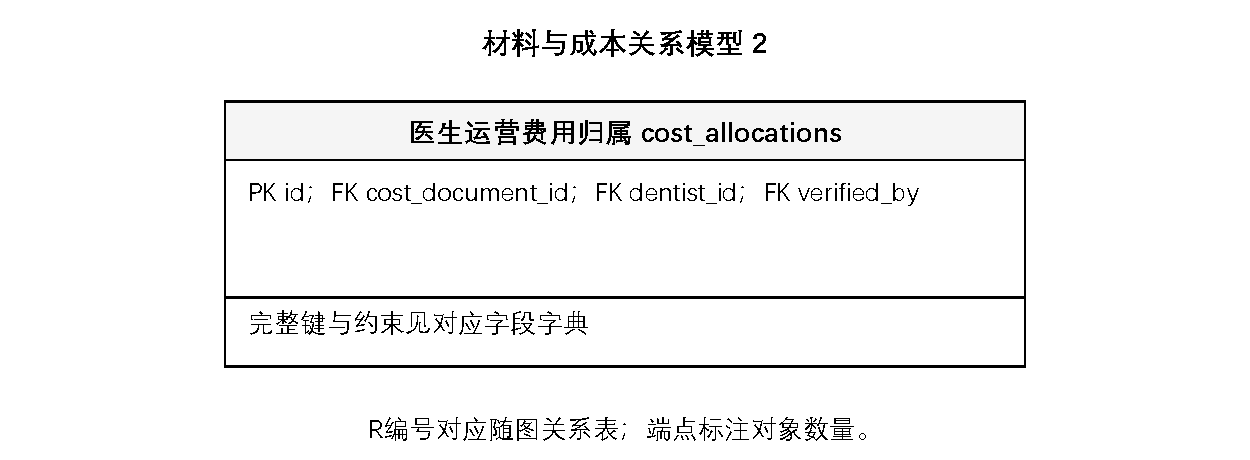
\includegraphics[width=\textwidth]{figures/er_18.pdf}
\caption{材料与成本关系模型 2}\label{er_18}\end{figure}
\begin{figure}[H]\centering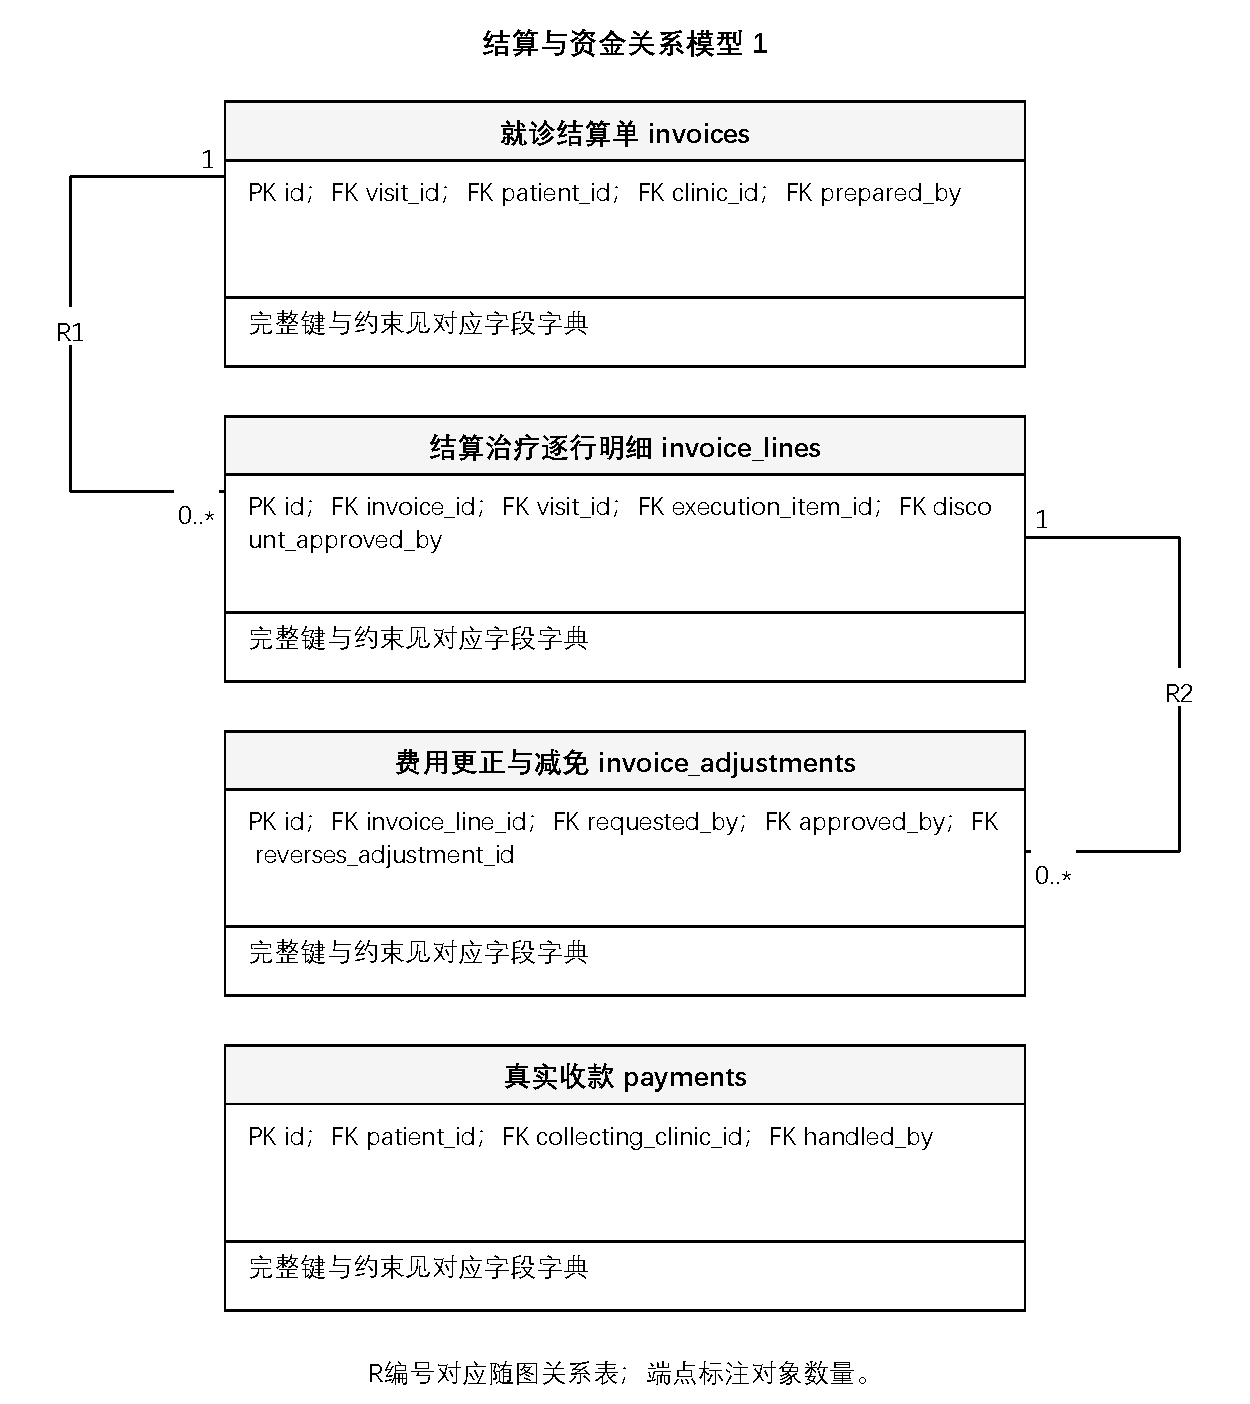
\includegraphics[width=\textwidth]{figures/er_19.pdf}
\caption{结算与资金关系模型 1}\label{er_19}\end{figure}
\par\noindent\begin{minipage}{\textwidth}
{\fontsize{10.5pt}{13.2pt}\selectfont\setlength{\tabcolsep}{0pt}\renewcommand{\arraystretch}{1.08}
\captionof{table}{结算与资金关系模型 1关联}\label{tab436}
\begin{tabular}{@{}p{1.240cm}@{\hspace{0.16cm}}p{10.040cm}@{\hspace{0.16cm}}p{3.840cm}@{}}
\toprule
\bfseries \Cell{编号} & \bfseries \Cell{外键联系} & \bfseries \Cell{父对象数/\allowbreak{}子对象数}\\\midrule
\Cell{R1} & \Cell{invoices ← invoice\_\allowbreak{}lines.\allowbreak{}invoice\_\allowbreak{}id} & \Cell{1 /\allowbreak{} 0.\allowbreak{}.\allowbreak{}*\allowbreak{}}\\[1pt]
\Cell{R2} & \Cell{invoice\_\allowbreak{}lines ← invoice\_\allowbreak{}adjustments.\allowbreak{}invoice\_\allowbreak{}line\_\allowbreak{}id} & \Cell{1 /\allowbreak{} 0.\allowbreak{}.\allowbreak{}*\allowbreak{}}\\[1pt]
\bottomrule\end{tabular}
}\end{minipage}\par\vspace{6pt}
\begin{figure}[H]\centering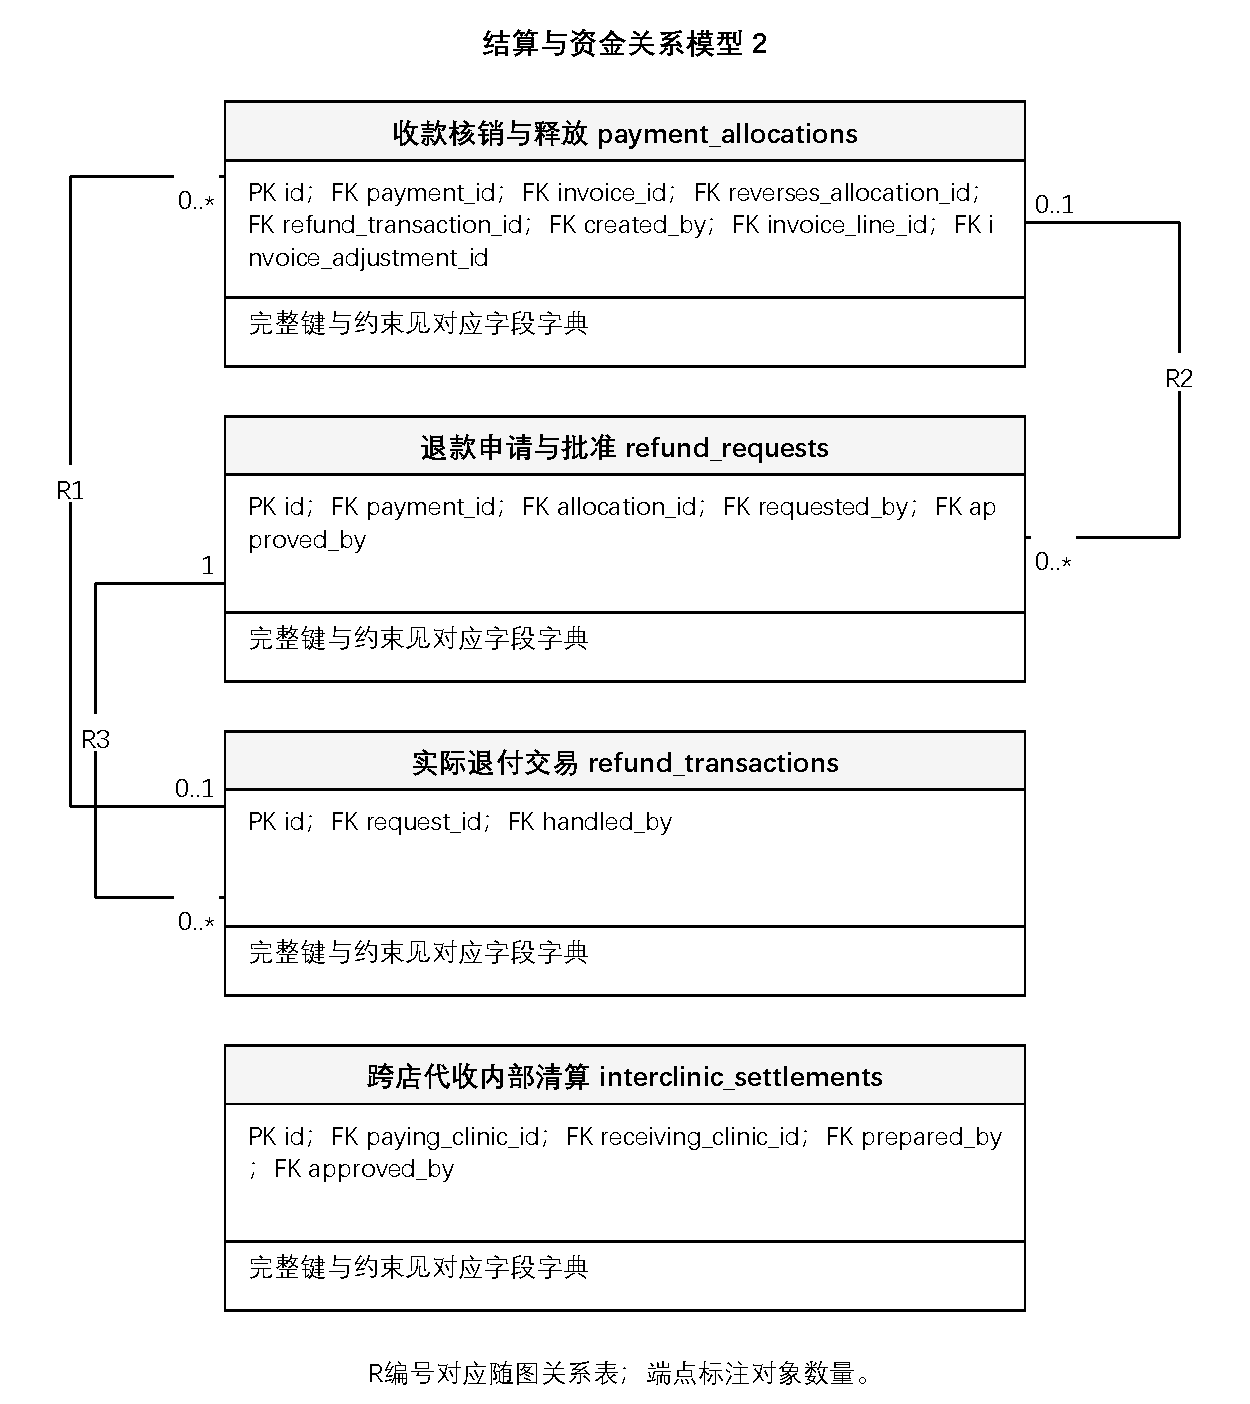
\includegraphics[width=\textwidth]{figures/er_20.pdf}
\caption{结算与资金关系模型 2}\label{er_20}\end{figure}
\par\noindent\begin{minipage}{\textwidth}
{\fontsize{10.5pt}{13.2pt}\selectfont\setlength{\tabcolsep}{0pt}\renewcommand{\arraystretch}{1.08}
\captionof{table}{结算与资金关系模型 2关联}\label{tab438}
\begin{tabular}{@{}p{1.240cm}@{\hspace{0.16cm}}p{10.040cm}@{\hspace{0.16cm}}p{3.840cm}@{}}
\toprule
\bfseries \Cell{编号} & \bfseries \Cell{外键联系} & \bfseries \Cell{父对象数/\allowbreak{}子对象数}\\\midrule
\Cell{R1} & \Cell{refund\_\allowbreak{}transactions ← payment\_\allowbreak{}allocations.\allowbreak{}refund\_\allowbreak{}transaction\_\allowbreak{}id} & \Cell{0.\allowbreak{}.\allowbreak{}1 /\allowbreak{} 0.\allowbreak{}.\allowbreak{}*\allowbreak{}}\\[1pt]
\Cell{R2} & \Cell{payment\_\allowbreak{}allocations ← refund\_\allowbreak{}requests.\allowbreak{}allocation\_\allowbreak{}id} & \Cell{0.\allowbreak{}.\allowbreak{}1 /\allowbreak{} 0.\allowbreak{}.\allowbreak{}*\allowbreak{}}\\[1pt]
\Cell{R3} & \Cell{refund\_\allowbreak{}requests ← refund\_\allowbreak{}transactions.\allowbreak{}request\_\allowbreak{}id} & \Cell{1 /\allowbreak{} 0.\allowbreak{}.\allowbreak{}*\allowbreak{}}\\[1pt]
\bottomrule\end{tabular}
}\end{minipage}\par\vspace{6pt}
\begin{figure}[H]\centering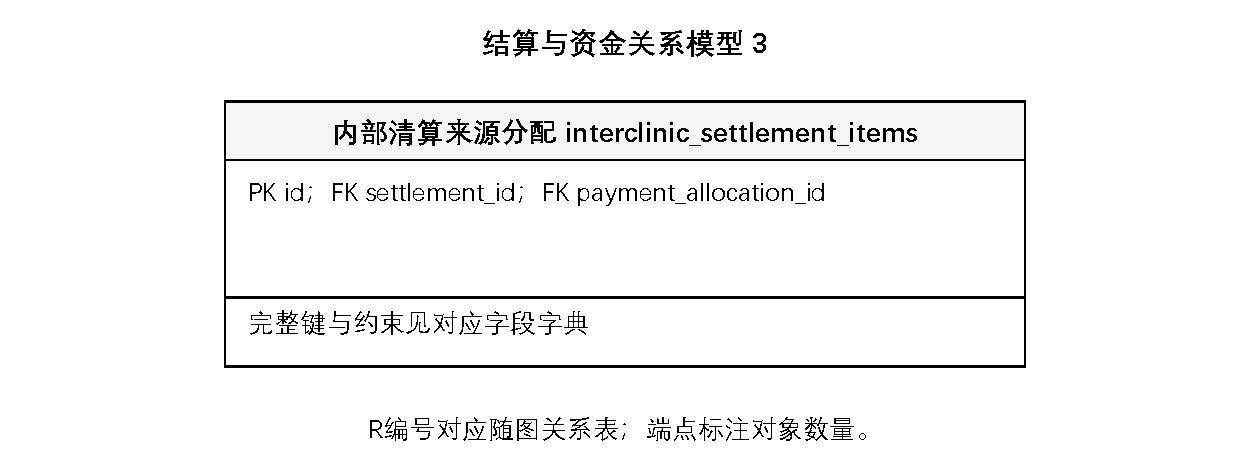
\includegraphics[width=\textwidth]{figures/er_21.pdf}
\caption{结算与资金关系模型 3}\label{er_21}\end{figure}
\begin{figure}[H]\centering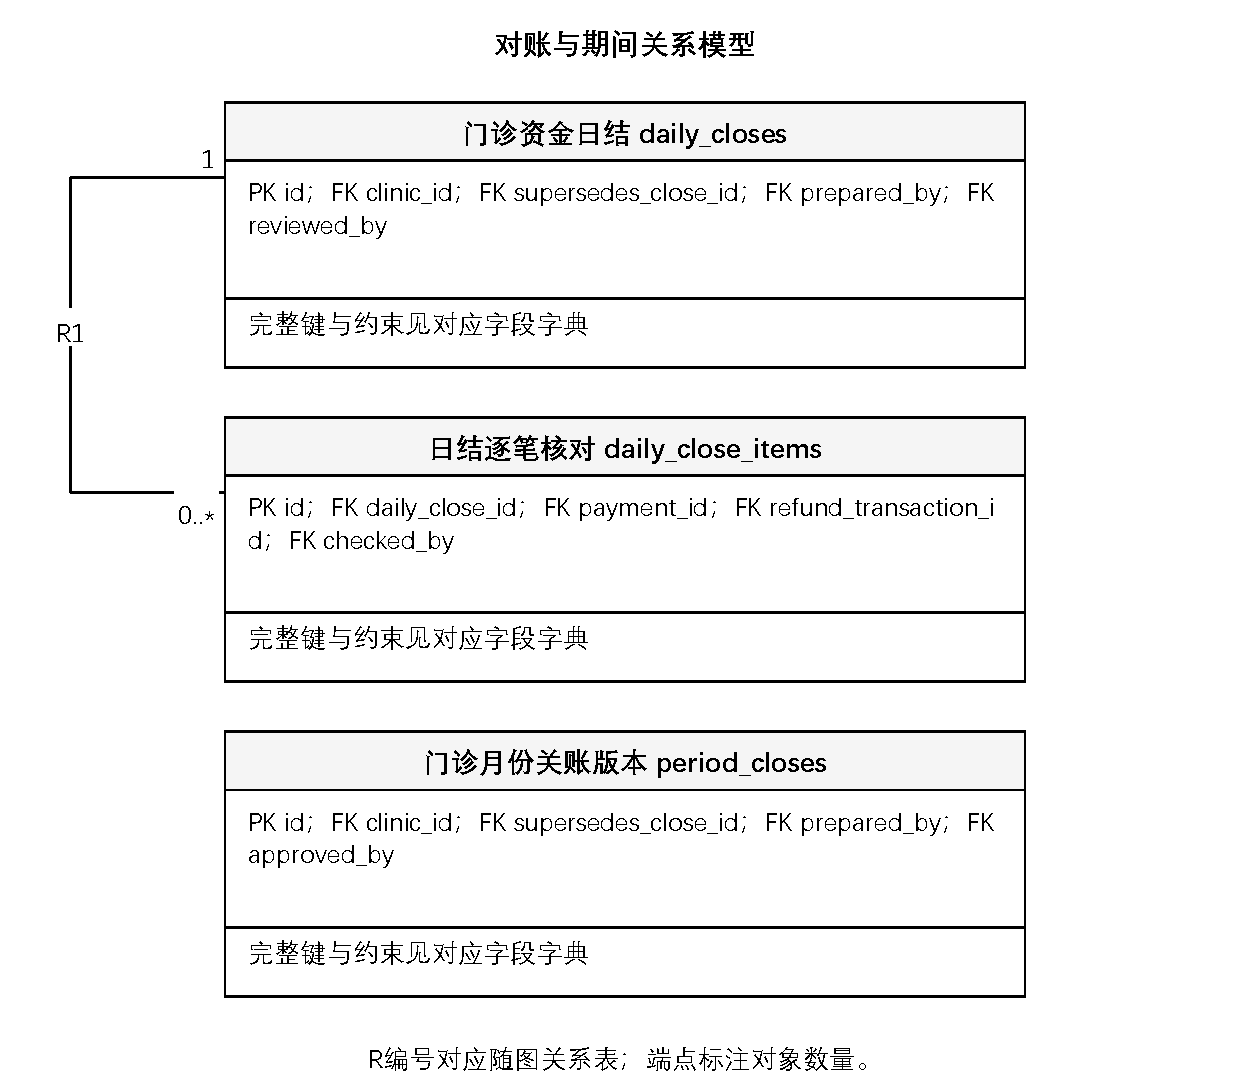
\includegraphics[width=\textwidth]{figures/er_22.pdf}
\caption{对账与期间关系模型}\label{er_22}\end{figure}
\par\noindent\begin{minipage}{\textwidth}
{\fontsize{10.5pt}{13.2pt}\selectfont\setlength{\tabcolsep}{0pt}\renewcommand{\arraystretch}{1.08}
\captionof{table}{对账与期间关系模型关联}\label{tab441}
\begin{tabular}{@{}p{1.240cm}@{\hspace{0.16cm}}p{10.040cm}@{\hspace{0.16cm}}p{3.840cm}@{}}
\toprule
\bfseries \Cell{编号} & \bfseries \Cell{外键联系} & \bfseries \Cell{父对象数/\allowbreak{}子对象数}\\\midrule
\Cell{R1} & \Cell{daily\_\allowbreak{}closes ← daily\_\allowbreak{}close\_\allowbreak{}items.\allowbreak{}daily\_\allowbreak{}close\_\allowbreak{}id} & \Cell{1 /\allowbreak{} 0.\allowbreak{}.\allowbreak{}*\allowbreak{}}\\[1pt]
\bottomrule\end{tabular}
}\end{minipage}\par\vspace{6pt}
\begin{figure}[H]\centering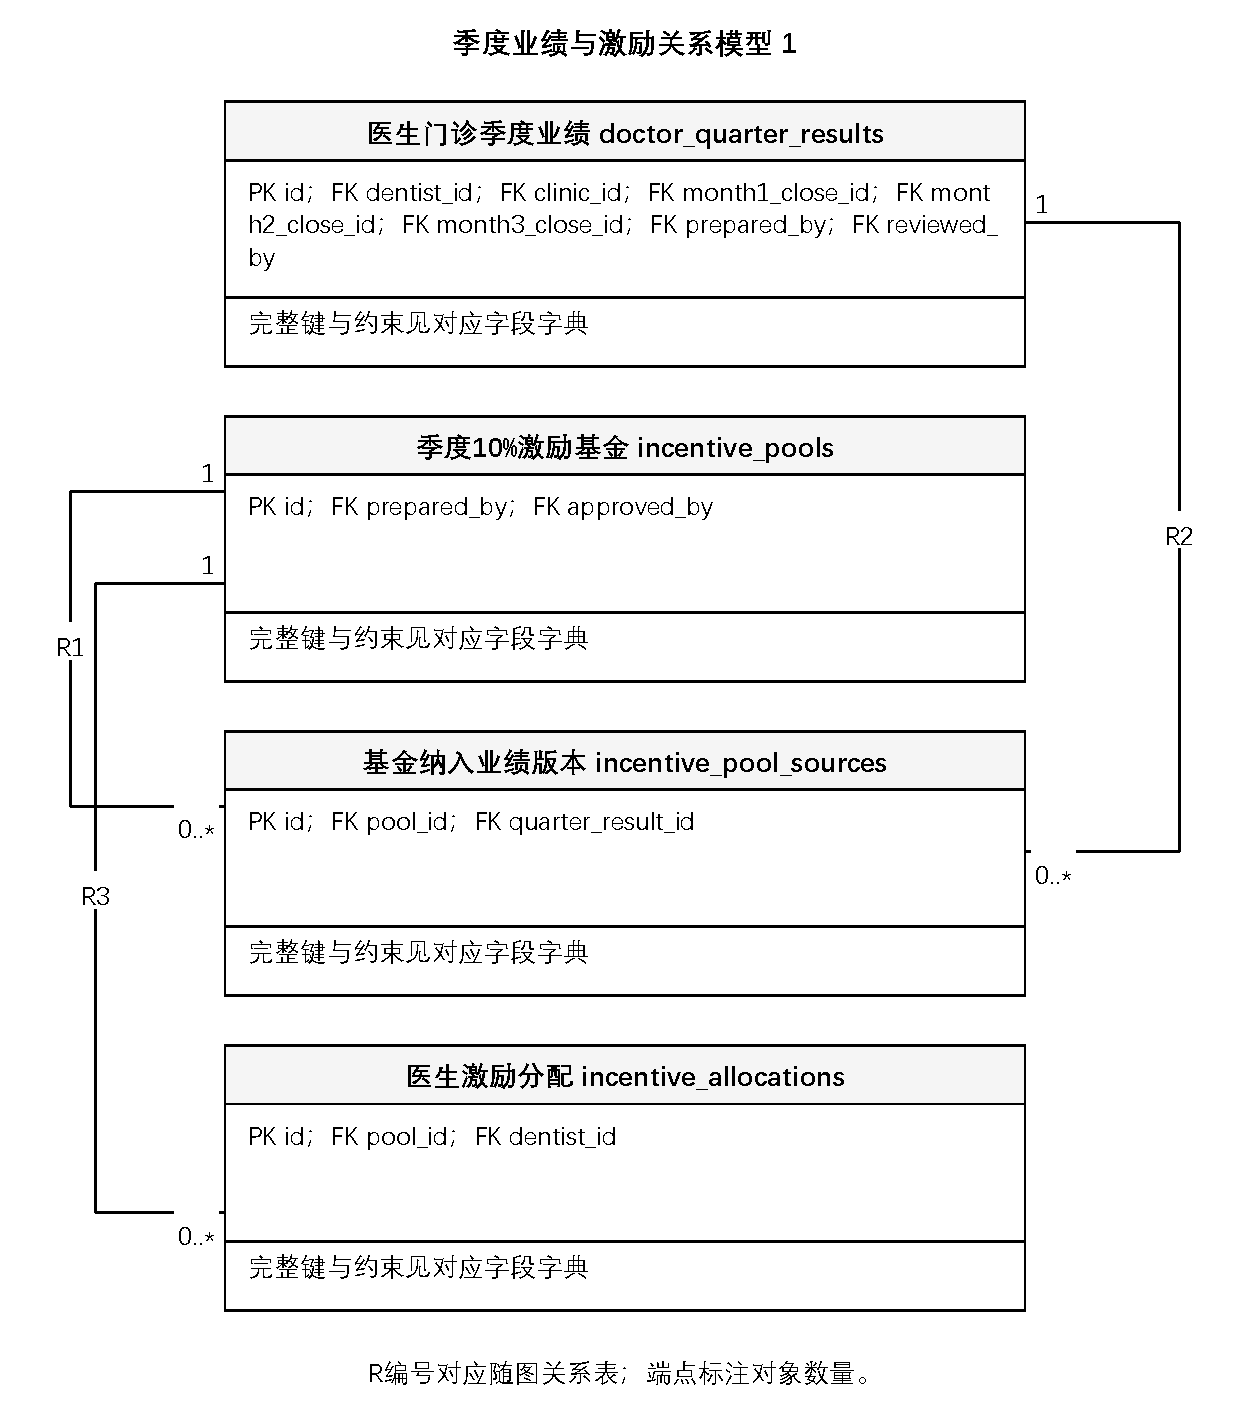
\includegraphics[width=\textwidth]{figures/er_23.pdf}
\caption{季度业绩与激励关系模型 1}\label{er_23}\end{figure}
\par\noindent\begin{minipage}{\textwidth}
{\fontsize{10.5pt}{13.2pt}\selectfont\setlength{\tabcolsep}{0pt}\renewcommand{\arraystretch}{1.08}
\captionof{table}{季度业绩与激励关系模型 1关联}\label{tab443}
\begin{tabular}{@{}p{1.240cm}@{\hspace{0.16cm}}p{10.040cm}@{\hspace{0.16cm}}p{3.840cm}@{}}
\toprule
\bfseries \Cell{编号} & \bfseries \Cell{外键联系} & \bfseries \Cell{父对象数/\allowbreak{}子对象数}\\\midrule
\Cell{R1} & \Cell{incentive\_\allowbreak{}pools ← incentive\_\allowbreak{}pool\_\allowbreak{}sources.\allowbreak{}pool\_\allowbreak{}id} & \Cell{1 /\allowbreak{} 0.\allowbreak{}.\allowbreak{}*\allowbreak{}}\\[1pt]
\Cell{R2} & \Cell{doctor\_\allowbreak{}quarter\_\allowbreak{}results ← incentive\_\allowbreak{}pool\_\allowbreak{}sources.\allowbreak{}quarter\_\allowbreak{}result\_\allowbreak{}id} & \Cell{1 /\allowbreak{} 0.\allowbreak{}.\allowbreak{}*\allowbreak{}}\\[1pt]
\Cell{R3} & \Cell{incentive\_\allowbreak{}pools ← incentive\_\allowbreak{}allocations.\allowbreak{}pool\_\allowbreak{}id} & \Cell{1 /\allowbreak{} 0.\allowbreak{}.\allowbreak{}*\allowbreak{}}\\[1pt]
\bottomrule\end{tabular}
}\end{minipage}\par\vspace{6pt}
\begin{figure}[H]\centering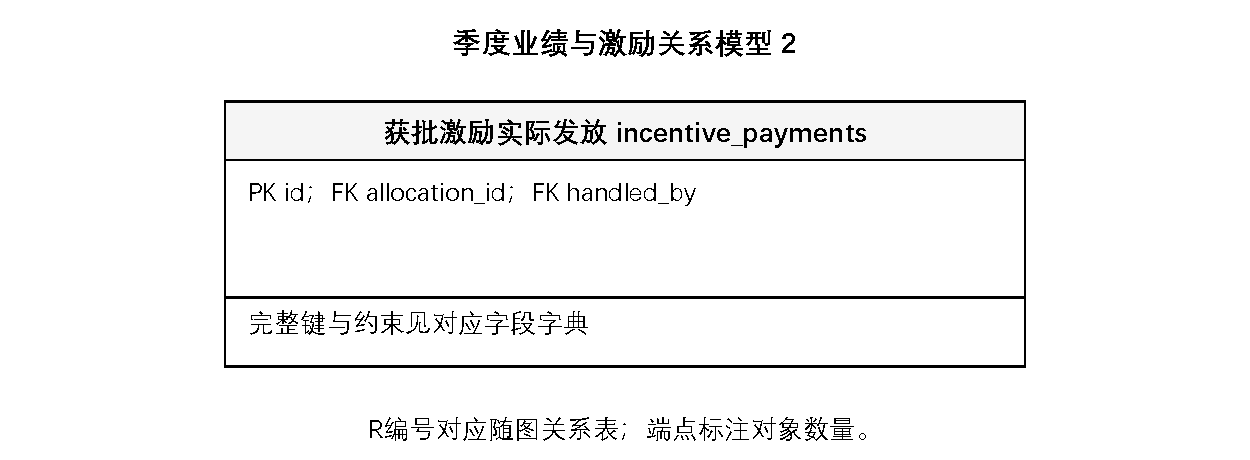
\includegraphics[width=\textwidth]{figures/er_24.pdf}
\caption{季度业绩与激励关系模型 2}\label{er_24}\end{figure}
\begin{figure}[H]\centering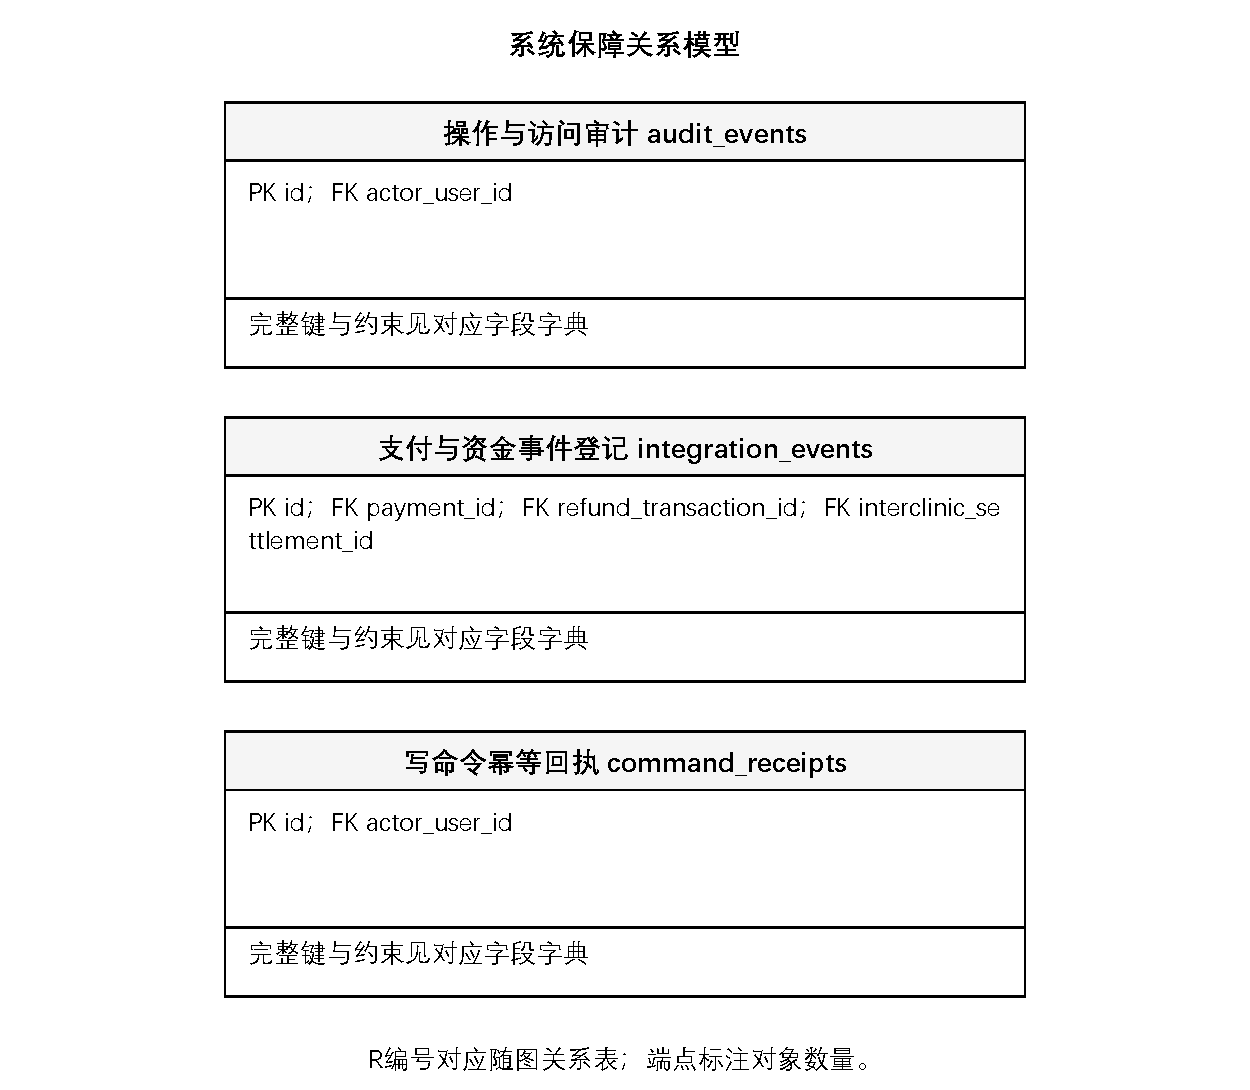
\includegraphics[width=\textwidth]{figures/er_25.pdf}
\caption{系统保障关系模型}\label{er_25}\end{figure}
{\fontsize{10.5pt}{13.2pt}\selectfont\setlength{\tabcolsep}{0pt}\renewcommand{\arraystretch}{1.08}
\begin{longtable}{@{}p{5.340cm}@{\hspace{0.16cm}}p{5.340cm}@{\hspace{0.16cm}}p{1.640cm}@{\hspace{0.16cm}}p{2.640cm}@{}}
\caption{完整外键关系}\label{tab446}\\
\toprule
\bfseries \Cell{引用字段} & \bfseries \Cell{目标键} & \bfseries \Cell{空值} & \bfseries \Cell{子端约束}\\\midrule
\endfirsthead
\toprule
\bfseries \Cell{引用字段} & \bfseries \Cell{目标键} & \bfseries \Cell{空值} & \bfseries \Cell{子端约束}\\\midrule
\endhead
\bottomrule\endlastfoot
\Cell{clinics.\allowbreak{}manager\_\allowbreak{}staff\_\allowbreak{}id} & \Cell{staff.\allowbreak{}id} & \Cell{非空} & \Cell{子端可多条}\\[1pt]
\Cell{users.\allowbreak{}staff\_\allowbreak{}id} & \Cell{staff.\allowbreak{}id} & \Cell{可空} & \Cell{子端唯一}\\[1pt]
\Cell{role\_\allowbreak{}assignments.\allowbreak{}user\_\allowbreak{}id} & \Cell{users.\allowbreak{}id} & \Cell{非空} & \Cell{子端可多条}\\[1pt]
\Cell{role\_\allowbreak{}assignments.\allowbreak{}clinic\_\allowbreak{}id} & \Cell{clinics.\allowbreak{}id} & \Cell{可空} & \Cell{子端可多条}\\[1pt]
\Cell{role\_\allowbreak{}assignments.\allowbreak{}approved\_\allowbreak{}by} & \Cell{users.\allowbreak{}id} & \Cell{非空} & \Cell{子端可多条}\\[1pt]
\Cell{patients.\allowbreak{}merged\_\allowbreak{}into\_\allowbreak{}patient\_\allowbreak{}id} & \Cell{patients.\allowbreak{}id} & \Cell{可空} & \Cell{子端可多条}\\[1pt]
\Cell{patients.\allowbreak{}allergy\_\allowbreak{}checked\_\allowbreak{}by} & \Cell{staff.\allowbreak{}id} & \Cell{可空} & \Cell{子端可多条}\\[1pt]
\Cell{patient\_\allowbreak{}access\_\allowbreak{}grants.\allowbreak{}user\_\allowbreak{}id} & \Cell{users.\allowbreak{}id} & \Cell{非空} & \Cell{子端可多条}\\[1pt]
\Cell{patient\_\allowbreak{}access\_\allowbreak{}grants.\allowbreak{}patient\_\allowbreak{}id} & \Cell{patients.\allowbreak{}id} & \Cell{非空} & \Cell{子端可多条}\\[1pt]
\Cell{patient\_\allowbreak{}access\_\allowbreak{}grants.\allowbreak{}verified\_\allowbreak{}by} & \Cell{users.\allowbreak{}id} & \Cell{非空} & \Cell{子端可多条}\\[1pt]
\Cell{patient\_\allowbreak{}allergies.\allowbreak{}patient\_\allowbreak{}id} & \Cell{patients.\allowbreak{}id} & \Cell{非空} & \Cell{子端可多条}\\[1pt]
\Cell{patient\_\allowbreak{}allergies.\allowbreak{}allergen\_\allowbreak{}id} & \Cell{allergens.\allowbreak{}id} & \Cell{可空} & \Cell{子端可多条}\\[1pt]
\Cell{patient\_\allowbreak{}allergies.\allowbreak{}recorded\_\allowbreak{}by} & \Cell{users.\allowbreak{}id} & \Cell{非空} & \Cell{子端可多条}\\[1pt]
\Cell{patient\_\allowbreak{}allergies.\allowbreak{}supersedes\_\allowbreak{}record\_\allowbreak{}id} & \Cell{patient\_\allowbreak{}allergies.\allowbreak{}id} & \Cell{可空} & \Cell{子端可多条}\\[1pt]
\Cell{patient\_\allowbreak{}allergies.\allowbreak{}reviewed\_\allowbreak{}by} & \Cell{staff.\allowbreak{}id} & \Cell{可空} & \Cell{子端可多条}\\[1pt]
\Cell{dentist\_\allowbreak{}qualifications.\allowbreak{}dentist\_\allowbreak{}id} & \Cell{staff.\allowbreak{}id} & \Cell{非空} & \Cell{子端可多条}\\[1pt]
\Cell{dentist\_\allowbreak{}qualifications.\allowbreak{}qualification\_\allowbreak{}id} & \Cell{qualifications.\allowbreak{}id} & \Cell{非空} & \Cell{子端可多条}\\[1pt]
\Cell{dentist\_\allowbreak{}qualifications.\allowbreak{}verified\_\allowbreak{}by} & \Cell{users.\allowbreak{}id} & \Cell{非空} & \Cell{子端可多条}\\[1pt]
\Cell{service\_\allowbreak{}qualifications.\allowbreak{}service\_\allowbreak{}id} & \Cell{services.\allowbreak{}id} & \Cell{非空} & \Cell{子端可多条}\\[1pt]
\Cell{service\_\allowbreak{}qualifications.\allowbreak{}qualification\_\allowbreak{}id} & \Cell{qualifications.\allowbreak{}id} & \Cell{非空} & \Cell{子端可多条}\\[1pt]
\Cell{service\_\allowbreak{}prices.\allowbreak{}service\_\allowbreak{}id} & \Cell{services.\allowbreak{}id} & \Cell{非空} & \Cell{子端可多条}\\[1pt]
\Cell{service\_\allowbreak{}prices.\allowbreak{}clinic\_\allowbreak{}id} & \Cell{clinics.\allowbreak{}id} & \Cell{可空} & \Cell{子端可多条}\\[1pt]
\Cell{service\_\allowbreak{}prices.\allowbreak{}approved\_\allowbreak{}by} & \Cell{users.\allowbreak{}id} & \Cell{非空} & \Cell{子端可多条}\\[1pt]
\Cell{chairs.\allowbreak{}clinic\_\allowbreak{}id} & \Cell{clinics.\allowbreak{}id} & \Cell{非空} & \Cell{子端可多条}\\[1pt]
\Cell{chair\_\allowbreak{}blocks.\allowbreak{}chair\_\allowbreak{}id} & \Cell{chairs.\allowbreak{}id} & \Cell{非空} & \Cell{子端可多条}\\[1pt]
\Cell{chair\_\allowbreak{}blocks.\allowbreak{}recorded\_\allowbreak{}by} & \Cell{users.\allowbreak{}id} & \Cell{非空} & \Cell{子端可多条}\\[1pt]
\Cell{doctor\_\allowbreak{}shifts.\allowbreak{}dentist\_\allowbreak{}id} & \Cell{staff.\allowbreak{}id} & \Cell{非空} & \Cell{子端可多条}\\[1pt]
\Cell{doctor\_\allowbreak{}shifts.\allowbreak{}clinic\_\allowbreak{}id} & \Cell{clinics.\allowbreak{}id} & \Cell{非空} & \Cell{子端可多条}\\[1pt]
\Cell{doctor\_\allowbreak{}shifts.\allowbreak{}published\_\allowbreak{}by} & \Cell{users.\allowbreak{}id} & \Cell{非空} & \Cell{子端可多条}\\[1pt]
\Cell{appointments.\allowbreak{}patient\_\allowbreak{}id} & \Cell{patients.\allowbreak{}id} & \Cell{非空} & \Cell{子端可多条}\\[1pt]
\Cell{appointments.\allowbreak{}clinic\_\allowbreak{}id} & \Cell{clinics.\allowbreak{}id} & \Cell{非空} & \Cell{子端可多条}\\[1pt]
\Cell{appointments.\allowbreak{}dentist\_\allowbreak{}id} & \Cell{staff.\allowbreak{}id} & \Cell{非空} & \Cell{子端可多条}\\[1pt]
\Cell{appointments.\allowbreak{}chair\_\allowbreak{}id} & \Cell{chairs.\allowbreak{}id} & \Cell{非空} & \Cell{子端可多条}\\[1pt]
\Cell{appointments.\allowbreak{}service\_\allowbreak{}id} & \Cell{services.\allowbreak{}id} & \Cell{非空} & \Cell{子端可多条}\\[1pt]
\Cell{appointments.\allowbreak{}shift\_\allowbreak{}id} & \Cell{doctor\_\allowbreak{}shifts.\allowbreak{}id} & \Cell{非空} & \Cell{子端可多条}\\[1pt]
\Cell{appointments.\allowbreak{}plan\_\allowbreak{}item\_\allowbreak{}id} & \Cell{plan\_\allowbreak{}items.\allowbreak{}id} & \Cell{可空} & \Cell{子端可多条}\\[1pt]
\Cell{appointments.\allowbreak{}created\_\allowbreak{}by} & \Cell{users.\allowbreak{}id} & \Cell{非空} & \Cell{子端可多条}\\[1pt]
\Cell{appointments.\allowbreak{}supersedes\_\allowbreak{}appointment\_\allowbreak{}id} & \Cell{appointments.\allowbreak{}id} & \Cell{可空} & \Cell{子端唯一}\\[1pt]
\Cell{appointments.\allowbreak{}root\_\allowbreak{}appointment\_\allowbreak{}id} & \Cell{appointments.\allowbreak{}id} & \Cell{可空} & \Cell{子端可多条}\\[1pt]
\Cell{appointments.\allowbreak{}request\_\allowbreak{}id} & \Cell{appointment\_\allowbreak{}requests.\allowbreak{}id} & \Cell{可空} & \Cell{子端可多条}\\[1pt]
\Cell{appointment\_\allowbreak{}events.\allowbreak{}appointment\_\allowbreak{}id} & \Cell{appointments.\allowbreak{}id} & \Cell{非空} & \Cell{子端可多条}\\[1pt]
\Cell{appointment\_\allowbreak{}events.\allowbreak{}actor\_\allowbreak{}user\_\allowbreak{}id} & \Cell{users.\allowbreak{}id} & \Cell{非空} & \Cell{子端可多条}\\[1pt]
\Cell{appointment\_\allowbreak{}events.\allowbreak{}replacement\_\allowbreak{}appointment\_\allowbreak{}id} & \Cell{appointments.\allowbreak{}id} & \Cell{可空} & \Cell{子端可多条}\\[1pt]
\Cell{booking\_\allowbreak{}holds.\allowbreak{}patient\_\allowbreak{}id} & \Cell{patients.\allowbreak{}id} & \Cell{非空} & \Cell{子端可多条}\\[1pt]
\Cell{booking\_\allowbreak{}holds.\allowbreak{}dentist\_\allowbreak{}id} & \Cell{staff.\allowbreak{}id} & \Cell{非空} & \Cell{子端可多条}\\[1pt]
\Cell{booking\_\allowbreak{}holds.\allowbreak{}chair\_\allowbreak{}id} & \Cell{chairs.\allowbreak{}id} & \Cell{非空} & \Cell{子端可多条}\\[1pt]
\Cell{booking\_\allowbreak{}holds.\allowbreak{}shift\_\allowbreak{}id} & \Cell{doctor\_\allowbreak{}shifts.\allowbreak{}id} & \Cell{非空} & \Cell{子端可多条}\\[1pt]
\Cell{booking\_\allowbreak{}holds.\allowbreak{}service\_\allowbreak{}id} & \Cell{services.\allowbreak{}id} & \Cell{非空} & \Cell{子端可多条}\\[1pt]
\Cell{booking\_\allowbreak{}holds.\allowbreak{}appointment\_\allowbreak{}id} & \Cell{appointments.\allowbreak{}id} & \Cell{可空} & \Cell{子端唯一}\\[1pt]
\Cell{booking\_\allowbreak{}holds.\allowbreak{}created\_\allowbreak{}by} & \Cell{users.\allowbreak{}id} & \Cell{非空} & \Cell{子端可多条}\\[1pt]
\Cell{waitlist\_\allowbreak{}entries.\allowbreak{}patient\_\allowbreak{}id} & \Cell{patients.\allowbreak{}id} & \Cell{非空} & \Cell{子端可多条}\\[1pt]
\Cell{waitlist\_\allowbreak{}entries.\allowbreak{}clinic\_\allowbreak{}id} & \Cell{clinics.\allowbreak{}id} & \Cell{非空} & \Cell{子端可多条}\\[1pt]
\Cell{waitlist\_\allowbreak{}entries.\allowbreak{}service\_\allowbreak{}id} & \Cell{services.\allowbreak{}id} & \Cell{非空} & \Cell{子端可多条}\\[1pt]
\Cell{waitlist\_\allowbreak{}entries.\allowbreak{}preferred\_\allowbreak{}dentist\_\allowbreak{}id} & \Cell{staff.\allowbreak{}id} & \Cell{可空} & \Cell{子端可多条}\\[1pt]
\Cell{waitlist\_\allowbreak{}entries.\allowbreak{}existing\_\allowbreak{}appointment\_\allowbreak{}id} & \Cell{appointments.\allowbreak{}id} & \Cell{可空} & \Cell{子端可多条}\\[1pt]
\Cell{waitlist\_\allowbreak{}entries.\allowbreak{}offered\_\allowbreak{}hold\_\allowbreak{}id} & \Cell{booking\_\allowbreak{}holds.\allowbreak{}id} & \Cell{可空} & \Cell{子端可多条}\\[1pt]
\Cell{waitlist\_\allowbreak{}entries.\allowbreak{}accepted\_\allowbreak{}appointment\_\allowbreak{}id} & \Cell{appointments.\allowbreak{}id} & \Cell{可空} & \Cell{子端可多条}\\[1pt]
\Cell{waitlist\_\allowbreak{}entries.\allowbreak{}request\_\allowbreak{}id} & \Cell{appointment\_\allowbreak{}requests.\allowbreak{}id} & \Cell{可空} & \Cell{子端可多条}\\[1pt]
\Cell{notification\_\allowbreak{}tasks.\allowbreak{}patient\_\allowbreak{}id} & \Cell{patients.\allowbreak{}id} & \Cell{非空} & \Cell{子端可多条}\\[1pt]
\Cell{notification\_\allowbreak{}tasks.\allowbreak{}appointment\_\allowbreak{}id} & \Cell{appointments.\allowbreak{}id} & \Cell{可空} & \Cell{子端可多条}\\[1pt]
\Cell{notification\_\allowbreak{}tasks.\allowbreak{}followup\_\allowbreak{}task\_\allowbreak{}id} & \Cell{followup\_\allowbreak{}tasks.\allowbreak{}id} & \Cell{可空} & \Cell{子端可多条}\\[1pt]
\Cell{notification\_\allowbreak{}tasks.\allowbreak{}owner\_\allowbreak{}user\_\allowbreak{}id} & \Cell{users.\allowbreak{}id} & \Cell{可空} & \Cell{子端可多条}\\[1pt]
\Cell{visits.\allowbreak{}appointment\_\allowbreak{}id} & \Cell{appointments.\allowbreak{}id} & \Cell{非空} & \Cell{子端唯一}\\[1pt]
\Cell{visits.\allowbreak{}patient\_\allowbreak{}id} & \Cell{patients.\allowbreak{}id} & \Cell{非空} & \Cell{子端可多条}\\[1pt]
\Cell{visits.\allowbreak{}clinic\_\allowbreak{}id} & \Cell{clinics.\allowbreak{}id} & \Cell{非空} & \Cell{子端可多条}\\[1pt]
\Cell{visits.\allowbreak{}attending\_\allowbreak{}dentist\_\allowbreak{}id} & \Cell{staff.\allowbreak{}id} & \Cell{非空} & \Cell{子端可多条}\\[1pt]
\Cell{treatment\_\allowbreak{}plans.\allowbreak{}patient\_\allowbreak{}id} & \Cell{patients.\allowbreak{}id} & \Cell{非空} & \Cell{子端可多条}\\[1pt]
\Cell{treatment\_\allowbreak{}plans.\allowbreak{}responsible\_\allowbreak{}dentist\_\allowbreak{}id} & \Cell{staff.\allowbreak{}id} & \Cell{非空} & \Cell{子端可多条}\\[1pt]
\Cell{plan\_\allowbreak{}versions.\allowbreak{}plan\_\allowbreak{}id} & \Cell{treatment\_\allowbreak{}plans.\allowbreak{}id} & \Cell{非空} & \Cell{子端可多条}\\[1pt]
\Cell{plan\_\allowbreak{}versions.\allowbreak{}prepared\_\allowbreak{}by} & \Cell{staff.\allowbreak{}id} & \Cell{非空} & \Cell{子端可多条}\\[1pt]
\Cell{plan\_\allowbreak{}items.\allowbreak{}plan\_\allowbreak{}version\_\allowbreak{}id} & \Cell{plan\_\allowbreak{}versions.\allowbreak{}id} & \Cell{非空} & \Cell{子端可多条}\\[1pt]
\Cell{plan\_\allowbreak{}items.\allowbreak{}service\_\allowbreak{}id} & \Cell{services.\allowbreak{}id} & \Cell{非空} & \Cell{子端可多条}\\[1pt]
\Cell{plan\_\allowbreak{}items.\allowbreak{}service\_\allowbreak{}price\_\allowbreak{}id} & \Cell{service\_\allowbreak{}prices.\allowbreak{}id} & \Cell{非空} & \Cell{子端可多条}\\[1pt]
\Cell{plan\_\allowbreak{}items.\allowbreak{}predecessor\_\allowbreak{}item\_\allowbreak{}id} & \Cell{plan\_\allowbreak{}items.\allowbreak{}id} & \Cell{可空} & \Cell{子端可多条}\\[1pt]
\Cell{consent\_\allowbreak{}records.\allowbreak{}plan\_\allowbreak{}version\_\allowbreak{}id} & \Cell{plan\_\allowbreak{}versions.\allowbreak{}id} & \Cell{非空} & \Cell{子端可多条}\\[1pt]
\Cell{consent\_\allowbreak{}records.\allowbreak{}patient\_\allowbreak{}id} & \Cell{patients.\allowbreak{}id} & \Cell{非空} & \Cell{子端可多条}\\[1pt]
\Cell{consent\_\allowbreak{}records.\allowbreak{}grant\_\allowbreak{}id} & \Cell{patient\_\allowbreak{}access\_\allowbreak{}grants.\allowbreak{}id} & \Cell{可空} & \Cell{子端可多条}\\[1pt]
\Cell{consent\_\allowbreak{}records.\allowbreak{}explained\_\allowbreak{}by} & \Cell{staff.\allowbreak{}id} & \Cell{非空} & \Cell{子端可多条}\\[1pt]
\Cell{treatment\_\allowbreak{}executions.\allowbreak{}visit\_\allowbreak{}id} & \Cell{visits.\allowbreak{}id} & \Cell{非空} & \Cell{子端可多条}\\[1pt]
\Cell{treatment\_\allowbreak{}executions.\allowbreak{}dentist\_\allowbreak{}id} & \Cell{staff.\allowbreak{}id} & \Cell{非空} & \Cell{子端可多条}\\[1pt]
\Cell{treatment\_\allowbreak{}executions.\allowbreak{}plan\_\allowbreak{}version\_\allowbreak{}id} & \Cell{plan\_\allowbreak{}versions.\allowbreak{}id} & \Cell{可空} & \Cell{子端可多条}\\[1pt]
\Cell{execution\_\allowbreak{}items.\allowbreak{}execution\_\allowbreak{}id} & \Cell{treatment\_\allowbreak{}executions.\allowbreak{}id} & \Cell{非空} & \Cell{子端可多条}\\[1pt]
\Cell{execution\_\allowbreak{}items.\allowbreak{}visit\_\allowbreak{}id} & \Cell{visits.\allowbreak{}id} & \Cell{非空} & \Cell{子端可多条}\\[1pt]
\Cell{execution\_\allowbreak{}items.\allowbreak{}plan\_\allowbreak{}item\_\allowbreak{}id} & \Cell{plan\_\allowbreak{}items.\allowbreak{}id} & \Cell{可空} & \Cell{子端可多条}\\[1pt]
\Cell{execution\_\allowbreak{}items.\allowbreak{}service\_\allowbreak{}id} & \Cell{services.\allowbreak{}id} & \Cell{非空} & \Cell{子端可多条}\\[1pt]
\Cell{execution\_\allowbreak{}items.\allowbreak{}performing\_\allowbreak{}dentist\_\allowbreak{}id} & \Cell{staff.\allowbreak{}id} & \Cell{非空} & \Cell{子端可多条}\\[1pt]
\Cell{execution\_\allowbreak{}items.\allowbreak{}service\_\allowbreak{}price\_\allowbreak{}id} & \Cell{service\_\allowbreak{}prices.\allowbreak{}id} & \Cell{非空} & \Cell{子端可多条}\\[1pt]
\Cell{clinical\_\allowbreak{}records.\allowbreak{}visit\_\allowbreak{}id} & \Cell{visits.\allowbreak{}id} & \Cell{非空} & \Cell{子端可多条}\\[1pt]
\Cell{clinical\_\allowbreak{}records.\allowbreak{}author\_\allowbreak{}dentist\_\allowbreak{}id} & \Cell{staff.\allowbreak{}id} & \Cell{非空} & \Cell{子端可多条}\\[1pt]
\Cell{record\_\allowbreak{}addenda.\allowbreak{}clinical\_\allowbreak{}record\_\allowbreak{}id} & \Cell{clinical\_\allowbreak{}records.\allowbreak{}id} & \Cell{非空} & \Cell{子端可多条}\\[1pt]
\Cell{record\_\allowbreak{}addenda.\allowbreak{}author\_\allowbreak{}dentist\_\allowbreak{}id} & \Cell{staff.\allowbreak{}id} & \Cell{非空} & \Cell{子端可多条}\\[1pt]
\Cell{material\_\allowbreak{}lots.\allowbreak{}clinic\_\allowbreak{}id} & \Cell{clinics.\allowbreak{}id} & \Cell{非空} & \Cell{子端可多条}\\[1pt]
\Cell{material\_\allowbreak{}lots.\allowbreak{}material\_\allowbreak{}id} & \Cell{materials.\allowbreak{}id} & \Cell{非空} & \Cell{子端可多条}\\[1pt]
\Cell{material\_\allowbreak{}lots.\allowbreak{}verified\_\allowbreak{}by} & \Cell{users.\allowbreak{}id} & \Cell{非空} & \Cell{子端可多条}\\[1pt]
\Cell{material\_\allowbreak{}consumptions.\allowbreak{}execution\_\allowbreak{}item\_\allowbreak{}id} & \Cell{execution\_\allowbreak{}items.\allowbreak{}id} & \Cell{非空} & \Cell{子端可多条}\\[1pt]
\Cell{material\_\allowbreak{}consumptions.\allowbreak{}lot\_\allowbreak{}id} & \Cell{material\_\allowbreak{}lots.\allowbreak{}id} & \Cell{非空} & \Cell{子端可多条}\\[1pt]
\Cell{material\_\allowbreak{}consumptions.\allowbreak{}reverses\_\allowbreak{}consumption\_\allowbreak{}id} & \Cell{material\_\allowbreak{}consumptions.\allowbreak{}id} & \Cell{可空} & \Cell{子端可多条}\\[1pt]
\Cell{material\_\allowbreak{}consumptions.\allowbreak{}recorded\_\allowbreak{}by} & \Cell{users.\allowbreak{}id} & \Cell{非空} & \Cell{子端可多条}\\[1pt]
\Cell{material\_\allowbreak{}consumptions.\allowbreak{}priced\_\allowbreak{}by} & \Cell{users.\allowbreak{}id} & \Cell{可空} & \Cell{子端可多条}\\[1pt]
\Cell{invoices.\allowbreak{}visit\_\allowbreak{}id} & \Cell{visits.\allowbreak{}id} & \Cell{非空} & \Cell{子端唯一}\\[1pt]
\Cell{invoices.\allowbreak{}patient\_\allowbreak{}id} & \Cell{patients.\allowbreak{}id} & \Cell{非空} & \Cell{子端可多条}\\[1pt]
\Cell{invoices.\allowbreak{}clinic\_\allowbreak{}id} & \Cell{clinics.\allowbreak{}id} & \Cell{非空} & \Cell{子端可多条}\\[1pt]
\Cell{invoices.\allowbreak{}prepared\_\allowbreak{}by} & \Cell{users.\allowbreak{}id} & \Cell{非空} & \Cell{子端可多条}\\[1pt]
\Cell{invoice\_\allowbreak{}lines.\allowbreak{}invoice\_\allowbreak{}id} & \Cell{invoices.\allowbreak{}id} & \Cell{非空} & \Cell{子端可多条}\\[1pt]
\Cell{invoice\_\allowbreak{}lines.\allowbreak{}visit\_\allowbreak{}id} & \Cell{visits.\allowbreak{}id} & \Cell{非空} & \Cell{子端可多条}\\[1pt]
\Cell{invoice\_\allowbreak{}lines.\allowbreak{}execution\_\allowbreak{}item\_\allowbreak{}id} & \Cell{execution\_\allowbreak{}items.\allowbreak{}id} & \Cell{非空} & \Cell{子端唯一}\\[1pt]
\Cell{invoice\_\allowbreak{}lines.\allowbreak{}discount\_\allowbreak{}approved\_\allowbreak{}by} & \Cell{users.\allowbreak{}id} & \Cell{可空} & \Cell{子端可多条}\\[1pt]
\Cell{invoice\_\allowbreak{}adjustments.\allowbreak{}invoice\_\allowbreak{}line\_\allowbreak{}id} & \Cell{invoice\_\allowbreak{}lines.\allowbreak{}id} & \Cell{非空} & \Cell{子端可多条}\\[1pt]
\Cell{invoice\_\allowbreak{}adjustments.\allowbreak{}requested\_\allowbreak{}by} & \Cell{users.\allowbreak{}id} & \Cell{非空} & \Cell{子端可多条}\\[1pt]
\Cell{invoice\_\allowbreak{}adjustments.\allowbreak{}approved\_\allowbreak{}by} & \Cell{users.\allowbreak{}id} & \Cell{非空} & \Cell{子端可多条}\\[1pt]
\Cell{invoice\_\allowbreak{}adjustments.\allowbreak{}reverses\_\allowbreak{}adjustment\_\allowbreak{}id} & \Cell{invoice\_\allowbreak{}adjustments.\allowbreak{}id} & \Cell{可空} & \Cell{子端唯一}\\[1pt]
\Cell{payments.\allowbreak{}patient\_\allowbreak{}id} & \Cell{patients.\allowbreak{}id} & \Cell{非空} & \Cell{子端可多条}\\[1pt]
\Cell{payments.\allowbreak{}collecting\_\allowbreak{}clinic\_\allowbreak{}id} & \Cell{clinics.\allowbreak{}id} & \Cell{非空} & \Cell{子端可多条}\\[1pt]
\Cell{payments.\allowbreak{}handled\_\allowbreak{}by} & \Cell{users.\allowbreak{}id} & \Cell{非空} & \Cell{子端可多条}\\[1pt]
\Cell{payment\_\allowbreak{}allocations.\allowbreak{}payment\_\allowbreak{}id} & \Cell{payments.\allowbreak{}id} & \Cell{非空} & \Cell{子端可多条}\\[1pt]
\Cell{payment\_\allowbreak{}allocations.\allowbreak{}invoice\_\allowbreak{}id} & \Cell{invoices.\allowbreak{}id} & \Cell{非空} & \Cell{子端可多条}\\[1pt]
\Cell{payment\_\allowbreak{}allocations.\allowbreak{}reverses\_\allowbreak{}allocation\_\allowbreak{}id} & \Cell{payment\_\allowbreak{}allocations.\allowbreak{}id} & \Cell{可空} & \Cell{子端可多条}\\[1pt]
\Cell{payment\_\allowbreak{}allocations.\allowbreak{}refund\_\allowbreak{}transaction\_\allowbreak{}id} & \Cell{refund\_\allowbreak{}transactions.\allowbreak{}id} & \Cell{可空} & \Cell{子端可多条}\\[1pt]
\Cell{payment\_\allowbreak{}allocations.\allowbreak{}created\_\allowbreak{}by} & \Cell{users.\allowbreak{}id} & \Cell{非空} & \Cell{子端可多条}\\[1pt]
\Cell{payment\_\allowbreak{}allocations.\allowbreak{}invoice\_\allowbreak{}line\_\allowbreak{}id} & \Cell{invoice\_\allowbreak{}lines.\allowbreak{}id} & \Cell{非空} & \Cell{子端可多条}\\[1pt]
\Cell{payment\_\allowbreak{}allocations.\allowbreak{}invoice\_\allowbreak{}adjustment\_\allowbreak{}id} & \Cell{invoice\_\allowbreak{}adjustments.\allowbreak{}id} & \Cell{可空} & \Cell{子端可多条}\\[1pt]
\Cell{refund\_\allowbreak{}requests.\allowbreak{}payment\_\allowbreak{}id} & \Cell{payments.\allowbreak{}id} & \Cell{非空} & \Cell{子端可多条}\\[1pt]
\Cell{refund\_\allowbreak{}requests.\allowbreak{}allocation\_\allowbreak{}id} & \Cell{payment\_\allowbreak{}allocations.\allowbreak{}id} & \Cell{可空} & \Cell{子端可多条}\\[1pt]
\Cell{refund\_\allowbreak{}requests.\allowbreak{}requested\_\allowbreak{}by} & \Cell{users.\allowbreak{}id} & \Cell{非空} & \Cell{子端可多条}\\[1pt]
\Cell{refund\_\allowbreak{}requests.\allowbreak{}approved\_\allowbreak{}by} & \Cell{users.\allowbreak{}id} & \Cell{可空} & \Cell{子端可多条}\\[1pt]
\Cell{refund\_\allowbreak{}transactions.\allowbreak{}request\_\allowbreak{}id} & \Cell{refund\_\allowbreak{}requests.\allowbreak{}id} & \Cell{非空} & \Cell{子端可多条}\\[1pt]
\Cell{refund\_\allowbreak{}transactions.\allowbreak{}handled\_\allowbreak{}by} & \Cell{users.\allowbreak{}id} & \Cell{非空} & \Cell{子端可多条}\\[1pt]
\Cell{daily\_\allowbreak{}closes.\allowbreak{}clinic\_\allowbreak{}id} & \Cell{clinics.\allowbreak{}id} & \Cell{非空} & \Cell{子端可多条}\\[1pt]
\Cell{daily\_\allowbreak{}closes.\allowbreak{}supersedes\_\allowbreak{}close\_\allowbreak{}id} & \Cell{daily\_\allowbreak{}closes.\allowbreak{}id} & \Cell{可空} & \Cell{子端可多条}\\[1pt]
\Cell{daily\_\allowbreak{}closes.\allowbreak{}prepared\_\allowbreak{}by} & \Cell{users.\allowbreak{}id} & \Cell{非空} & \Cell{子端可多条}\\[1pt]
\Cell{daily\_\allowbreak{}closes.\allowbreak{}reviewed\_\allowbreak{}by} & \Cell{users.\allowbreak{}id} & \Cell{可空} & \Cell{子端可多条}\\[1pt]
\Cell{daily\_\allowbreak{}close\_\allowbreak{}items.\allowbreak{}daily\_\allowbreak{}close\_\allowbreak{}id} & \Cell{daily\_\allowbreak{}closes.\allowbreak{}id} & \Cell{非空} & \Cell{子端可多条}\\[1pt]
\Cell{daily\_\allowbreak{}close\_\allowbreak{}items.\allowbreak{}payment\_\allowbreak{}id} & \Cell{payments.\allowbreak{}id} & \Cell{可空} & \Cell{子端可多条}\\[1pt]
\Cell{daily\_\allowbreak{}close\_\allowbreak{}items.\allowbreak{}refund\_\allowbreak{}transaction\_\allowbreak{}id} & \Cell{refund\_\allowbreak{}transactions.\allowbreak{}id} & \Cell{可空} & \Cell{子端可多条}\\[1pt]
\Cell{daily\_\allowbreak{}close\_\allowbreak{}items.\allowbreak{}checked\_\allowbreak{}by} & \Cell{users.\allowbreak{}id} & \Cell{非空} & \Cell{子端可多条}\\[1pt]
\Cell{cost\_\allowbreak{}documents.\allowbreak{}clinic\_\allowbreak{}id} & \Cell{clinics.\allowbreak{}id} & \Cell{非空} & \Cell{子端可多条}\\[1pt]
\Cell{cost\_\allowbreak{}documents.\allowbreak{}reverses\_\allowbreak{}document\_\allowbreak{}id} & \Cell{cost\_\allowbreak{}documents.\allowbreak{}id} & \Cell{可空} & \Cell{子端可多条}\\[1pt]
\Cell{cost\_\allowbreak{}documents.\allowbreak{}prepared\_\allowbreak{}by} & \Cell{users.\allowbreak{}id} & \Cell{非空} & \Cell{子端可多条}\\[1pt]
\Cell{cost\_\allowbreak{}documents.\allowbreak{}reviewed\_\allowbreak{}by} & \Cell{users.\allowbreak{}id} & \Cell{可空} & \Cell{子端可多条}\\[1pt]
\Cell{cost\_\allowbreak{}allocations.\allowbreak{}cost\_\allowbreak{}document\_\allowbreak{}id} & \Cell{cost\_\allowbreak{}documents.\allowbreak{}id} & \Cell{非空} & \Cell{子端可多条}\\[1pt]
\Cell{cost\_\allowbreak{}allocations.\allowbreak{}dentist\_\allowbreak{}id} & \Cell{staff.\allowbreak{}id} & \Cell{非空} & \Cell{子端可多条}\\[1pt]
\Cell{cost\_\allowbreak{}allocations.\allowbreak{}verified\_\allowbreak{}by} & \Cell{users.\allowbreak{}id} & \Cell{非空} & \Cell{子端可多条}\\[1pt]
\Cell{period\_\allowbreak{}closes.\allowbreak{}clinic\_\allowbreak{}id} & \Cell{clinics.\allowbreak{}id} & \Cell{非空} & \Cell{子端可多条}\\[1pt]
\Cell{period\_\allowbreak{}closes.\allowbreak{}supersedes\_\allowbreak{}close\_\allowbreak{}id} & \Cell{period\_\allowbreak{}closes.\allowbreak{}id} & \Cell{可空} & \Cell{子端可多条}\\[1pt]
\Cell{period\_\allowbreak{}closes.\allowbreak{}prepared\_\allowbreak{}by} & \Cell{users.\allowbreak{}id} & \Cell{非空} & \Cell{子端可多条}\\[1pt]
\Cell{period\_\allowbreak{}closes.\allowbreak{}approved\_\allowbreak{}by} & \Cell{users.\allowbreak{}id} & \Cell{可空} & \Cell{子端可多条}\\[1pt]
\Cell{doctor\_\allowbreak{}quarter\_\allowbreak{}results.\allowbreak{}dentist\_\allowbreak{}id} & \Cell{staff.\allowbreak{}id} & \Cell{非空} & \Cell{子端可多条}\\[1pt]
\Cell{doctor\_\allowbreak{}quarter\_\allowbreak{}results.\allowbreak{}clinic\_\allowbreak{}id} & \Cell{clinics.\allowbreak{}id} & \Cell{非空} & \Cell{子端可多条}\\[1pt]
\Cell{doctor\_\allowbreak{}quarter\_\allowbreak{}results.\allowbreak{}month1\_\allowbreak{}close\_\allowbreak{}id} & \Cell{period\_\allowbreak{}closes.\allowbreak{}id} & \Cell{可空} & \Cell{子端可多条}\\[1pt]
\Cell{doctor\_\allowbreak{}quarter\_\allowbreak{}results.\allowbreak{}month2\_\allowbreak{}close\_\allowbreak{}id} & \Cell{period\_\allowbreak{}closes.\allowbreak{}id} & \Cell{可空} & \Cell{子端可多条}\\[1pt]
\Cell{doctor\_\allowbreak{}quarter\_\allowbreak{}results.\allowbreak{}month3\_\allowbreak{}close\_\allowbreak{}id} & \Cell{period\_\allowbreak{}closes.\allowbreak{}id} & \Cell{可空} & \Cell{子端可多条}\\[1pt]
\Cell{doctor\_\allowbreak{}quarter\_\allowbreak{}results.\allowbreak{}prepared\_\allowbreak{}by} & \Cell{users.\allowbreak{}id} & \Cell{非空} & \Cell{子端可多条}\\[1pt]
\Cell{doctor\_\allowbreak{}quarter\_\allowbreak{}results.\allowbreak{}reviewed\_\allowbreak{}by} & \Cell{users.\allowbreak{}id} & \Cell{可空} & \Cell{子端可多条}\\[1pt]
\Cell{incentive\_\allowbreak{}pools.\allowbreak{}prepared\_\allowbreak{}by} & \Cell{users.\allowbreak{}id} & \Cell{非空} & \Cell{子端可多条}\\[1pt]
\Cell{incentive\_\allowbreak{}pools.\allowbreak{}approved\_\allowbreak{}by} & \Cell{users.\allowbreak{}id} & \Cell{可空} & \Cell{子端可多条}\\[1pt]
\Cell{incentive\_\allowbreak{}pool\_\allowbreak{}sources.\allowbreak{}pool\_\allowbreak{}id} & \Cell{incentive\_\allowbreak{}pools.\allowbreak{}id} & \Cell{非空} & \Cell{子端可多条}\\[1pt]
\Cell{incentive\_\allowbreak{}pool\_\allowbreak{}sources.\allowbreak{}quarter\_\allowbreak{}result\_\allowbreak{}id} & \Cell{doctor\_\allowbreak{}quarter\_\allowbreak{}results.\allowbreak{}id} & \Cell{非空} & \Cell{子端可多条}\\[1pt]
\Cell{incentive\_\allowbreak{}allocations.\allowbreak{}pool\_\allowbreak{}id} & \Cell{incentive\_\allowbreak{}pools.\allowbreak{}id} & \Cell{非空} & \Cell{子端可多条}\\[1pt]
\Cell{incentive\_\allowbreak{}allocations.\allowbreak{}dentist\_\allowbreak{}id} & \Cell{staff.\allowbreak{}id} & \Cell{非空} & \Cell{子端可多条}\\[1pt]
\Cell{incentive\_\allowbreak{}payments.\allowbreak{}allocation\_\allowbreak{}id} & \Cell{incentive\_\allowbreak{}allocations.\allowbreak{}id} & \Cell{非空} & \Cell{子端可多条}\\[1pt]
\Cell{incentive\_\allowbreak{}payments.\allowbreak{}handled\_\allowbreak{}by} & \Cell{users.\allowbreak{}id} & \Cell{非空} & \Cell{子端可多条}\\[1pt]
\Cell{interclinic\_\allowbreak{}settlements.\allowbreak{}paying\_\allowbreak{}clinic\_\allowbreak{}id} & \Cell{clinics.\allowbreak{}id} & \Cell{非空} & \Cell{子端可多条}\\[1pt]
\Cell{interclinic\_\allowbreak{}settlements.\allowbreak{}receiving\_\allowbreak{}clinic\_\allowbreak{}id} & \Cell{clinics.\allowbreak{}id} & \Cell{非空} & \Cell{子端可多条}\\[1pt]
\Cell{interclinic\_\allowbreak{}settlements.\allowbreak{}prepared\_\allowbreak{}by} & \Cell{users.\allowbreak{}id} & \Cell{非空} & \Cell{子端可多条}\\[1pt]
\Cell{interclinic\_\allowbreak{}settlements.\allowbreak{}approved\_\allowbreak{}by} & \Cell{users.\allowbreak{}id} & \Cell{可空} & \Cell{子端可多条}\\[1pt]
\Cell{interclinic\_\allowbreak{}settlement\_\allowbreak{}items.\allowbreak{}settlement\_\allowbreak{}id} & \Cell{interclinic\_\allowbreak{}settlements.\allowbreak{}id} & \Cell{非空} & \Cell{子端可多条}\\[1pt]
\Cell{interclinic\_\allowbreak{}settlement\_\allowbreak{}items.\allowbreak{}payment\_\allowbreak{}allocation\_\allowbreak{}id} & \Cell{payment\_\allowbreak{}allocations.\allowbreak{}id} & \Cell{非空} & \Cell{子端可多条}\\[1pt]
\Cell{followup\_\allowbreak{}tasks.\allowbreak{}patient\_\allowbreak{}id} & \Cell{patients.\allowbreak{}id} & \Cell{非空} & \Cell{子端可多条}\\[1pt]
\Cell{followup\_\allowbreak{}tasks.\allowbreak{}source\_\allowbreak{}visit\_\allowbreak{}id} & \Cell{visits.\allowbreak{}id} & \Cell{非空} & \Cell{子端可多条}\\[1pt]
\Cell{followup\_\allowbreak{}tasks.\allowbreak{}plan\_\allowbreak{}item\_\allowbreak{}id} & \Cell{plan\_\allowbreak{}items.\allowbreak{}id} & \Cell{可空} & \Cell{子端可多条}\\[1pt]
\Cell{followup\_\allowbreak{}tasks.\allowbreak{}responsible\_\allowbreak{}dentist\_\allowbreak{}id} & \Cell{staff.\allowbreak{}id} & \Cell{非空} & \Cell{子端可多条}\\[1pt]
\Cell{followup\_\allowbreak{}tasks.\allowbreak{}target\_\allowbreak{}clinic\_\allowbreak{}id} & \Cell{clinics.\allowbreak{}id} & \Cell{非空} & \Cell{子端可多条}\\[1pt]
\Cell{followup\_\allowbreak{}tasks.\allowbreak{}assigned\_\allowbreak{}user\_\allowbreak{}id} & \Cell{users.\allowbreak{}id} & \Cell{非空} & \Cell{子端可多条}\\[1pt]
\Cell{followup\_\allowbreak{}tasks.\allowbreak{}next\_\allowbreak{}appointment\_\allowbreak{}id} & \Cell{appointments.\allowbreak{}id} & \Cell{可空} & \Cell{子端可多条}\\[1pt]
\Cell{followup\_\allowbreak{}tasks.\allowbreak{}receiving\_\allowbreak{}visit\_\allowbreak{}id} & \Cell{visits.\allowbreak{}id} & \Cell{可空} & \Cell{子端可多条}\\[1pt]
\Cell{followup\_\allowbreak{}tasks.\allowbreak{}receiving\_\allowbreak{}dentist\_\allowbreak{}id} & \Cell{staff.\allowbreak{}id} & \Cell{可空} & \Cell{子端可多条}\\[1pt]
\Cell{audit\_\allowbreak{}events.\allowbreak{}actor\_\allowbreak{}user\_\allowbreak{}id} & \Cell{users.\allowbreak{}id} & \Cell{可空} & \Cell{子端可多条}\\[1pt]
\Cell{integration\_\allowbreak{}events.\allowbreak{}payment\_\allowbreak{}id} & \Cell{payments.\allowbreak{}id} & \Cell{可空} & \Cell{子端可多条}\\[1pt]
\Cell{integration\_\allowbreak{}events.\allowbreak{}refund\_\allowbreak{}transaction\_\allowbreak{}id} & \Cell{refund\_\allowbreak{}transactions.\allowbreak{}id} & \Cell{可空} & \Cell{子端可多条}\\[1pt]
\Cell{integration\_\allowbreak{}events.\allowbreak{}interclinic\_\allowbreak{}settlement\_\allowbreak{}id} & \Cell{interclinic\_\allowbreak{}settlements.\allowbreak{}id} & \Cell{可空} & \Cell{子端可多条}\\[1pt]
\Cell{doctor\_\allowbreak{}shift\_\allowbreak{}services.\allowbreak{}shift\_\allowbreak{}id} & \Cell{doctor\_\allowbreak{}shifts.\allowbreak{}id} & \Cell{非空} & \Cell{子端可多条}\\[1pt]
\Cell{doctor\_\allowbreak{}shift\_\allowbreak{}services.\allowbreak{}service\_\allowbreak{}id} & \Cell{services.\allowbreak{}id} & \Cell{非空} & \Cell{子端可多条}\\[1pt]
\Cell{assignment\_\allowbreak{}permissions.\allowbreak{}role\_\allowbreak{}assignment\_\allowbreak{}id} & \Cell{role\_\allowbreak{}assignments.\allowbreak{}id} & \Cell{非空} & \Cell{子端可多条}\\[1pt]
\Cell{command\_\allowbreak{}receipts.\allowbreak{}actor\_\allowbreak{}user\_\allowbreak{}id} & \Cell{users.\allowbreak{}id} & \Cell{可空} & \Cell{子端可多条}\\[1pt]
\Cell{appointment\_\allowbreak{}requests.\allowbreak{}patient\_\allowbreak{}id} & \Cell{patients.\allowbreak{}id} & \Cell{非空} & \Cell{子端可多条}\\[1pt]
\Cell{appointment\_\allowbreak{}requests.\allowbreak{}preferred\_\allowbreak{}clinic\_\allowbreak{}id} & \Cell{clinics.\allowbreak{}id} & \Cell{可空} & \Cell{子端可多条}\\[1pt]
\Cell{appointment\_\allowbreak{}requests.\allowbreak{}service\_\allowbreak{}id} & \Cell{services.\allowbreak{}id} & \Cell{可空} & \Cell{子端可多条}\\[1pt]
\Cell{appointment\_\allowbreak{}requests.\allowbreak{}created\_\allowbreak{}by} & \Cell{users.\allowbreak{}id} & \Cell{非空} & \Cell{子端可多条}\\[1pt]
\Cell{appointment\_\allowbreak{}requests.\allowbreak{}owner\_\allowbreak{}user\_\allowbreak{}id} & \Cell{users.\allowbreak{}id} & \Cell{可空} & \Cell{子端可多条}\\[1pt]
\Cell{appointment\_\allowbreak{}requests.\allowbreak{}scheduled\_\allowbreak{}appointment\_\allowbreak{}id} & \Cell{appointments.\allowbreak{}id} & \Cell{可空} & \Cell{子端可多条}\\[1pt]
\Cell{resource\_\allowbreak{}reservations.\allowbreak{}patient\_\allowbreak{}id} & \Cell{patients.\allowbreak{}id} & \Cell{非空} & \Cell{子端可多条}\\[1pt]
\Cell{resource\_\allowbreak{}reservations.\allowbreak{}clinic\_\allowbreak{}id} & \Cell{clinics.\allowbreak{}id} & \Cell{非空} & \Cell{子端可多条}\\[1pt]
\Cell{resource\_\allowbreak{}reservations.\allowbreak{}service\_\allowbreak{}id} & \Cell{services.\allowbreak{}id} & \Cell{非空} & \Cell{子端可多条}\\[1pt]
\Cell{resource\_\allowbreak{}reservations.\allowbreak{}doctor\_\allowbreak{}id} & \Cell{staff.\allowbreak{}id} & \Cell{非空} & \Cell{子端可多条}\\[1pt]
\Cell{appointments.\allowbreak{}reservation\_\allowbreak{}id} & \Cell{resource\_\allowbreak{}reservations.\allowbreak{}id} & \Cell{非空} & \Cell{子端唯一}\\[1pt]
\Cell{booking\_\allowbreak{}holds.\allowbreak{}reservation\_\allowbreak{}id} & \Cell{resource\_\allowbreak{}reservations.\allowbreak{}id} & \Cell{非空} & \Cell{子端唯一}\\[1pt]
\Cell{treatment\_\allowbreak{}references.\allowbreak{}booking\_\allowbreak{}service\_\allowbreak{}id} & \Cell{services.\allowbreak{}id} & \Cell{可空} & \Cell{子端可多条}\\[1pt]
\end{longtable}
}
\par\noindent\begin{minipage}{\textwidth}
{\fontsize{10.5pt}{13.2pt}\selectfont\setlength{\tabcolsep}{0pt}\renewcommand{\arraystretch}{1.08}
\captionof{table}{同一业务归属的复合外键}\label{tab447}
\begin{tabular}{@{}p{5.540cm}@{\hspace{0.16cm}}p{5.540cm}@{\hspace{0.16cm}}p{4.040cm}@{}}
\toprule
\bfseries \Cell{引用列组} & \bfseries \Cell{目标唯一列组} & \bfseries \Cell{作用}\\\midrule
\Cell{execution\_\allowbreak{}items(\allowbreak{}execution\_\allowbreak{}id,\allowbreak{}visit\_\allowbreak{}id)\allowbreak{}} & \Cell{treatment\_\allowbreak{}executions(\allowbreak{}id,\allowbreak{}visit\_\allowbreak{}id)\allowbreak{}} & \Cell{同时约束所属就诊或患者，不能只验证每个单列ID存在。}\\[1pt]
\Cell{invoices(\allowbreak{}visit\_\allowbreak{}id,\allowbreak{}patient\_\allowbreak{}id,\allowbreak{}clinic\_\allowbreak{}id)\allowbreak{}} & \Cell{visits(\allowbreak{}id,\allowbreak{}patient\_\allowbreak{}id,\allowbreak{}clinic\_\allowbreak{}id)\allowbreak{}} & \Cell{同时约束所属就诊或患者，不能只验证每个单列ID存在。}\\[1pt]
\Cell{invoice\_\allowbreak{}lines(\allowbreak{}invoice\_\allowbreak{}id,\allowbreak{}visit\_\allowbreak{}id)\allowbreak{}} & \Cell{invoices(\allowbreak{}id,\allowbreak{}visit\_\allowbreak{}id)\allowbreak{}} & \Cell{同时约束所属就诊或患者，不能只验证每个单列ID存在。}\\[1pt]
\Cell{invoice\_\allowbreak{}lines(\allowbreak{}execution\_\allowbreak{}item\_\allowbreak{}id,\allowbreak{}visit\_\allowbreak{}id)\allowbreak{}} & \Cell{execution\_\allowbreak{}items(\allowbreak{}id,\allowbreak{}visit\_\allowbreak{}id)\allowbreak{}} & \Cell{同时约束所属就诊或患者，不能只验证每个单列ID存在。}\\[1pt]
\Cell{payment\_\allowbreak{}allocations(\allowbreak{}invoice\_\allowbreak{}line\_\allowbreak{}id,\allowbreak{}invoice\_\allowbreak{}id)\allowbreak{}} & \Cell{invoice\_\allowbreak{}lines(\allowbreak{}id,\allowbreak{}invoice\_\allowbreak{}id)\allowbreak{}} & \Cell{同时约束所属就诊或患者，不能只验证每个单列ID存在。}\\[1pt]
\Cell{resource\_\allowbreak{}reservations(\allowbreak{}chair\_\allowbreak{}id,\allowbreak{}clinic\_\allowbreak{}id)\allowbreak{}} & \Cell{chairs(\allowbreak{}id,\allowbreak{}clinic\_\allowbreak{}id)\allowbreak{}} & \Cell{牙椅必须属于占用记录的门诊。}\\[1pt]
\Cell{resource\_\allowbreak{}reservations(\allowbreak{}shift\_\allowbreak{}id,\allowbreak{}clinic\_\allowbreak{}id,\allowbreak{}doctor\_\allowbreak{}id)\allowbreak{}} & \Cell{doctor\_\allowbreak{}shifts(\allowbreak{}id,\allowbreak{}clinic\_\allowbreak{}id,\allowbreak{}dentist\_\allowbreak{}id)\allowbreak{}} & \Cell{班次必须属于相同门诊和医生；doctor\_\allowbreak{}id对应班次的dentist\_\allowbreak{}id。}\\[1pt]
\bottomrule\end{tabular}
}\end{minipage}\par\vspace{6pt}
\subsection{必要字段字典}
NULL表示该字段允许为空，NN表示非空，PK表示主键，FK表示外键，U表示单列唯一。复合唯一、时间排斥及跨表不变量在表后约束中给出。事件及财务事实保留来源，公共字段仍按表列明，避免在开发时遗漏。\par
\Needspace{639pt}
\subsubsection{门诊（clinics）}
保存ADC门诊位置、主管和营业信息。\par
\par\noindent\begin{minipage}{\textwidth}
{\fontsize{10.5pt}{13.2pt}\selectfont\setlength{\tabcolsep}{0pt}\renewcommand{\arraystretch}{1.08}
\captionof{table}{clinics字段}\label{tab452}
\begin{tabular}{@{}p{3.940cm}@{\hspace{0.16cm}}p{2.740cm}@{\hspace{0.16cm}}p{3.140cm}@{\hspace{0.16cm}}p{5.140cm}@{}}
\toprule
\bfseries \Cell{字段} & \bfseries \Cell{类型} & \bfseries \Cell{键与空值} & \bfseries \Cell{含义及限制}\\\midrule
\Cell{id} & \Cell{UUID} & \Cell{NN；PK} & \Cell{稳定全局标识，不承载业务顺序}\\[1pt]
\Cell{clinic\_\allowbreak{}no} & \Cell{TEXT} & \Cell{NN} & \Cell{连锁内稳定门诊编号}\\[1pt]
\Cell{name} & \Cell{TEXT} & \Cell{NN} & \Cell{门诊名称}\\[1pt]
\Cell{address} & \Cell{TEXT} & \Cell{NN} & \Cell{邮政地址}\\[1pt]
\Cell{manager\_\allowbreak{}staff\_\allowbreak{}id} & \Cell{UUID} & \Cell{NN；FK→\\staff.\allowbreak{}id} & \Cell{负责本门诊的主管员工}\\[1pt]
\Cell{phone} & \Cell{TEXT} & \Cell{NN} & \Cell{门诊联系电话}\\[1pt]
\Cell{email} & \Cell{TEXT} & \Cell{NN} & \Cell{门诊联系邮箱}\\[1pt]
\Cell{floor\_\allowbreak{}area\_\allowbreak{}m2} & \Cell{NUMERIC(\allowbreak{}18,\allowbreak{}4)\allowbreak{}} & \Cell{NN} & \Cell{办公面积，平方米}\\[1pt]
\Cell{time\_\allowbreak{}zone} & \Cell{TEXT} & \Cell{NN} & \Cell{业务时区，采用Asia/\allowbreak{}Shanghai}\\[1pt]
\Cell{opens\_\allowbreak{}at} & \Cell{TIME} & \Cell{NN} & \Cell{正常营业开始}\\[1pt]
\Cell{closes\_\allowbreak{}at} & \Cell{TIME} & \Cell{NN} & \Cell{正常营业结束}\\[1pt]
\Cell{status} & \Cell{TEXT} & \Cell{NN} & \Cell{preparing、active、suspended、closed}\\[1pt]
\Cell{opened\_\allowbreak{}on} & \Cell{DATE} & \Cell{NN} & \Cell{门诊实际进入经营范围日期}\\[1pt]
\Cell{closed\_\allowbreak{}on} & \Cell{DATE} & \Cell{NULL} & \Cell{永久结束经营日期；仍经营为空}\\[1pt]
\Cell{created\_\allowbreak{}at} & \Cell{TIMESTAMPTZ} & \Cell{NN} & \Cell{创建时间，UTC保存}\\[1pt]
\Cell{updated\_\allowbreak{}at} & \Cell{TIMESTAMPTZ} & \Cell{NN} & \Cell{当前草稿或状态最后变更时间}\\[1pt]
\Cell{row\_\allowbreak{}version} & \Cell{INTEGER} & \Cell{NN} & \Cell{并发版本，成功修改递增}\\[1pt]
\bottomrule\end{tabular}
}\end{minipage}\par\vspace{6pt}
约束：UNIQUE(\allowbreak{}clinic\_\allowbreak{}no)\allowbreak{}；row\_\allowbreak{}version>\allowbreak{}=\allowbreak{}1；floor\_\allowbreak{}area\_\allowbreak{}m2>\allowbreak{}0；opens\_\allowbreak{}at<\allowbreak{}closes\_\allowbreak{}at；closed\_\allowbreak{}on IS NULL OR closed\_\allowbreak{}on>\allowbreak{}=\allowbreak{}opened\_\allowbreak{}on；主管任职和manager权限须覆盖门诊及生效期间。停业不删除历史业务。；季度范围逐月依据opened\_\allowbreak{}on和closed\_\allowbreak{}on构造；整月不在经营有效期的排除有来源，不能因没有月结快照就默认为未经营或金额为零。\par
\Needspace{552pt}
\subsubsection{员工与医生档案（staff）}
记录医生个人资料，并作为跨门诊执业、资格与业绩的稳定主体。\par
\par\noindent\begin{minipage}{\textwidth}
{\fontsize{10.5pt}{13.2pt}\selectfont\setlength{\tabcolsep}{0pt}\renewcommand{\arraystretch}{1.08}
\captionof{table}{staff字段}\label{tab456}
\begin{tabular}{@{}p{3.940cm}@{\hspace{0.16cm}}p{2.740cm}@{\hspace{0.16cm}}p{3.140cm}@{\hspace{0.16cm}}p{5.140cm}@{}}
\toprule
\bfseries \Cell{字段} & \bfseries \Cell{类型} & \bfseries \Cell{键与空值} & \bfseries \Cell{含义及限制}\\\midrule
\Cell{id} & \Cell{UUID} & \Cell{NN；PK} & \Cell{稳定全局标识，不承载业务顺序}\\[1pt]
\Cell{staff\_\allowbreak{}no} & \Cell{TEXT} & \Cell{NN} & \Cell{员工编号}\\[1pt]
\Cell{name} & \Cell{TEXT} & \Cell{NN} & \Cell{姓名}\\[1pt]
\Cell{birth\_\allowbreak{}date} & \Cell{DATE} & \Cell{NN} & \Cell{出生日期}\\[1pt]
\Cell{home\_\allowbreak{}address\_\allowbreak{}ref} & \Cell{TEXT} & \Cell{NN} & \Cell{家庭住址的加密受控存储引用}\\[1pt]
\Cell{phone} & \Cell{TEXT} & \Cell{NN} & \Cell{联系电话}\\[1pt]
\Cell{email} & \Cell{TEXT} & \Cell{NN} & \Cell{电子邮箱}\\[1pt]
\Cell{staff\_\allowbreak{}type} & \Cell{TEXT} & \Cell{NN} & \Cell{dentist、support、operations}\\[1pt]
\Cell{employment\_\allowbreak{}status} & \Cell{TEXT} & \Cell{NN} & \Cell{employed、leave、terminated}\\[1pt]
\Cell{joined\_\allowbreak{}on} & \Cell{DATE} & \Cell{NN} & \Cell{入职日期}\\[1pt]
\Cell{left\_\allowbreak{}on} & \Cell{DATE} & \Cell{NULL} & \Cell{离职日期}\\[1pt]
\Cell{created\_\allowbreak{}at} & \Cell{TIMESTAMPTZ} & \Cell{NN} & \Cell{创建时间，UTC保存}\\[1pt]
\Cell{updated\_\allowbreak{}at} & \Cell{TIMESTAMPTZ} & \Cell{NN} & \Cell{当前草稿或状态最后变更时间}\\[1pt]
\Cell{row\_\allowbreak{}version} & \Cell{INTEGER} & \Cell{NN} & \Cell{并发版本，成功修改递增}\\[1pt]
\bottomrule\end{tabular}
}\end{minipage}\par\vspace{6pt}
约束：UNIQUE(\allowbreak{}staff\_\allowbreak{}no)\allowbreak{}；row\_\allowbreak{}version>\allowbreak{}=\allowbreak{}1；left\_\allowbreak{}on IS NULL OR left\_\allowbreak{}on>\allowbreak{}=\allowbreak{}joined\_\allowbreak{}on；出生日期和家庭住址仅供必要人事核验，不进入顾客号源或普通前台视图。医生是否可执业另外核查资格及任务授权。\par
\Needspace{482pt}
\subsubsection{登录账号（users）}
认证身份与患者档案、员工档案分离。\par
\par\noindent\begin{minipage}{\textwidth}
{\fontsize{10.5pt}{13.2pt}\selectfont\setlength{\tabcolsep}{0pt}\renewcommand{\arraystretch}{1.08}
\captionof{table}{users字段}\label{tab460}
\begin{tabular}{@{}p{3.940cm}@{\hspace{0.16cm}}p{2.740cm}@{\hspace{0.16cm}}p{3.140cm}@{\hspace{0.16cm}}p{5.140cm}@{}}
\toprule
\bfseries \Cell{字段} & \bfseries \Cell{类型} & \bfseries \Cell{键与空值} & \bfseries \Cell{含义及限制}\\\midrule
\Cell{id} & \Cell{UUID} & \Cell{NN；PK} & \Cell{稳定全局标识，不承载业务顺序}\\[1pt]
\Cell{login\_\allowbreak{}name} & \Cell{TEXT} & \Cell{NN} & \Cell{规范化登录名}\\[1pt]
\Cell{password\_\allowbreak{}hash} & \Cell{TEXT} & \Cell{NN} & \Cell{密码的不可逆安全散列}\\[1pt]
\Cell{principal\_\allowbreak{}type} & \Cell{TEXT} & \Cell{NN} & \Cell{customer或staff}\\[1pt]
\Cell{staff\_\allowbreak{}id} & \Cell{UUID} & \Cell{NULL；FK→\\staff.\allowbreak{}id} & \Cell{员工主体；customer账号为空}\\[1pt]
\Cell{display\_\allowbreak{}name} & \Cell{TEXT} & \Cell{NN} & \Cell{账号显示姓名，不能单独作为身份核验依据}\\[1pt]
\Cell{status} & \Cell{TEXT} & \Cell{NN} & \Cell{active、locked、disabled}\\[1pt]
\Cell{session\_\allowbreak{}version} & \Cell{INTEGER} & \Cell{NN} & \Cell{撤销已有会话的版本}\\[1pt]
\Cell{created\_\allowbreak{}at} & \Cell{TIMESTAMPTZ} & \Cell{NN} & \Cell{创建时间，UTC保存}\\[1pt]
\Cell{updated\_\allowbreak{}at} & \Cell{TIMESTAMPTZ} & \Cell{NN} & \Cell{当前草稿或状态最后变更时间}\\[1pt]
\Cell{row\_\allowbreak{}version} & \Cell{INTEGER} & \Cell{NN} & \Cell{并发版本，成功修改递增}\\[1pt]
\bottomrule\end{tabular}
}\end{minipage}\par\vspace{6pt}
约束：UNIQUE(\allowbreak{}login\_\allowbreak{}name)\allowbreak{}；UNIQUE(\allowbreak{}staff\_\allowbreak{}id)\allowbreak{}；row\_\allowbreak{}version>\allowbreak{}=\allowbreak{}1；(\allowbreak{}principal\_\allowbreak{}type=\allowbreak{}'staff' AND staff\_\allowbreak{}id IS NOT NULL)\allowbreak{} OR (\allowbreak{}principal\_\allowbreak{}type=\allowbreak{}'customer' AND staff\_\allowbreak{}id IS NULL)\allowbreak{}；session\_\allowbreak{}version>\allowbreak{}=\allowbreak{}1；顾客可通过经核验授权管理本人或家庭成员；共用手机号不推导医疗资料权限。离职停用不删除历史经办和签署。\par
\Needspace{523pt}
\subsubsection{岗位与门诊授权（role\_assignments）}
定义员工在时间与门诊范围内承担的任务。\par
\par\noindent\begin{minipage}{\textwidth}
{\fontsize{10.5pt}{13.2pt}\selectfont\setlength{\tabcolsep}{0pt}\renewcommand{\arraystretch}{1.08}
\captionof{table}{role\_assignments字段}\label{tab464}
\begin{tabular}{@{}p{3.940cm}@{\hspace{0.16cm}}p{2.740cm}@{\hspace{0.16cm}}p{3.140cm}@{\hspace{0.16cm}}p{5.140cm}@{}}
\toprule
\bfseries \Cell{字段} & \bfseries \Cell{类型} & \bfseries \Cell{键与空值} & \bfseries \Cell{含义及限制}\\\midrule
\Cell{id} & \Cell{UUID} & \Cell{NN；PK} & \Cell{稳定全局标识，不承载业务顺序}\\[1pt]
\Cell{user\_\allowbreak{}id} & \Cell{UUID} & \Cell{NN；FK→\\users.\allowbreak{}id} & \Cell{员工账号}\\[1pt]
\Cell{role\_\allowbreak{}code} & \Cell{TEXT} & \Cell{NN} & \Cell{front、doctor、manager、hq}\\[1pt]
\Cell{clinic\_\allowbreak{}id} & \Cell{UUID} & \Cell{NULL；FK→\\clinics.\allowbreak{}id} & \Cell{门诊范围；仅总部全链授权可空}\\[1pt]
\Cell{valid\_\allowbreak{}from} & \Cell{DATE} & \Cell{NN} & \Cell{生效日}\\[1pt]
\Cell{valid\_\allowbreak{}until} & \Cell{DATE} & \Cell{NULL} & \Cell{终止日}\\[1pt]
\Cell{approved\_\allowbreak{}by} & \Cell{UUID} & \Cell{NN；FK→\\users.\allowbreak{}id} & \Cell{授权批准账号}\\[1pt]
\Cell{approval\_\allowbreak{}ref} & \Cell{TEXT} & \Cell{NN} & \Cell{任职或授权凭据}\\[1pt]
\Cell{status} & \Cell{TEXT} & \Cell{NN} & \Cell{active、revoked、expired}\\[1pt]
\Cell{created\_\allowbreak{}at} & \Cell{TIMESTAMPTZ} & \Cell{NN} & \Cell{创建时间，UTC保存}\\[1pt]
\Cell{updated\_\allowbreak{}at} & \Cell{TIMESTAMPTZ} & \Cell{NN} & \Cell{当前草稿或状态最后变更时间}\\[1pt]
\Cell{row\_\allowbreak{}version} & \Cell{INTEGER} & \Cell{NN} & \Cell{并发版本，成功修改递增}\\[1pt]
\bottomrule\end{tabular}
}\end{minipage}\par\vspace{6pt}
约束：UNIQUE(\allowbreak{}user\_\allowbreak{}id,\allowbreak{}role\_\allowbreak{}code,\allowbreak{}clinic\_\allowbreak{}id,\allowbreak{}valid\_\allowbreak{}from)\allowbreak{}；row\_\allowbreak{}version>\allowbreak{}=\allowbreak{}1；valid\_\allowbreak{}until IS NULL OR valid\_\allowbreak{}until>\allowbreak{}=\allowbreak{}valid\_\allowbreak{}from；role\_\allowbreak{}code=\allowbreak{}'hq' OR clinic\_\allowbreak{}id IS NOT NULL；总部是组织内部岗位；制单与审批还按自然员工回避，不能以切换账号规避。医生角色不自动替代专业资格。\par
\Needspace{216pt}
\subsubsection{患者主档（patients）}
保存患者身份、联系资料和逐项过敏核对状态。\par
{\fontsize{10.5pt}{13.2pt}\selectfont\setlength{\tabcolsep}{0pt}\renewcommand{\arraystretch}{1.08}
\begin{longtable}{@{}p{3.940cm}@{\hspace{0.16cm}}p{2.740cm}@{\hspace{0.16cm}}p{3.140cm}@{\hspace{0.16cm}}p{5.140cm}@{}}
\caption{patients字段}\label{tab468}\\
\toprule
\bfseries \Cell{字段} & \bfseries \Cell{类型} & \bfseries \Cell{键与空值} & \bfseries \Cell{含义及限制}\\\midrule
\endfirsthead
\toprule
\bfseries \Cell{字段} & \bfseries \Cell{类型} & \bfseries \Cell{键与空值} & \bfseries \Cell{含义及限制}\\\midrule
\endhead
\bottomrule\endlastfoot
\Cell{id} & \Cell{UUID} & \Cell{NN；PK} & \Cell{稳定全局标识，不承载业务顺序}\\[1pt]
\Cell{patient\_\allowbreak{}no} & \Cell{TEXT} & \Cell{NN} & \Cell{全连锁患者编号}\\[1pt]
\Cell{name} & \Cell{TEXT} & \Cell{NN} & \Cell{实际就诊人姓名}\\[1pt]
\Cell{birth\_\allowbreak{}date} & \Cell{DATE} & \Cell{NN} & \Cell{出生日期}\\[1pt]
\Cell{billing\_\allowbreak{}address} & \Cell{TEXT} & \Cell{NN} & \Cell{账单地址}\\[1pt]
\Cell{phone} & \Cell{TEXT} & \Cell{NN} & \Cell{联系电话}\\[1pt]
\Cell{email} & \Cell{TEXT} & \Cell{NULL} & \Cell{可选电子邮箱}\\[1pt]
\Cell{emergency\_\allowbreak{}contact\_\allowbreak{}name} & \Cell{TEXT} & \Cell{NN} & \Cell{紧急联系人姓名}\\[1pt]
\Cell{emergency\_\allowbreak{}contact\_\allowbreak{}phone} & \Cell{TEXT} & \Cell{NN} & \Cell{紧急联系人电话}\\[1pt]
\Cell{identity\_\allowbreak{}evidence\_\allowbreak{}ref} & \Cell{TEXT} & \Cell{NULL} & \Cell{受控身份核验依据}\\[1pt]
\Cell{verification\_\allowbreak{}status} & \Cell{TEXT} & \Cell{NN} & \Cell{draft、verified、merged}\\[1pt]
\Cell{merged\_\allowbreak{}into\_\allowbreak{}patient\_\allowbreak{}id} & \Cell{UUID} & \Cell{NULL；FK→\\patients.\allowbreak{}id} & \Cell{归并后保留的患者主档}\\[1pt]
\Cell{allergy\_\allowbreak{}status} & \Cell{TEXT} & \Cell{NN} & \Cell{unknown、none\_\allowbreak{}reported、known}\\[1pt]
\Cell{allergy\_\allowbreak{}checked\_\allowbreak{}at} & \Cell{TIMESTAMPTZ} & \Cell{NULL} & \Cell{最近一次过敏核对时间}\\[1pt]
\Cell{allergy\_\allowbreak{}checked\_\allowbreak{}by} & \Cell{UUID} & \Cell{NULL；FK→\\staff.\allowbreak{}id} & \Cell{最近核对员工}\\[1pt]
\Cell{contact\_\allowbreak{}allowed} & \Cell{BOOLEAN} & \Cell{NN} & \Cell{是否允许所选方式的服务通知}\\[1pt]
\Cell{contact\_\allowbreak{}channel} & \Cell{TEXT} & \Cell{NN} & \Cell{app、sms、phone、email}\\[1pt]
\Cell{allergy\_\allowbreak{}review\_\allowbreak{}version} & \Cell{INTEGER} & \Cell{NN} & \Cell{当前有效过敏声明版本；至少为1}\\[1pt]
\Cell{created\_\allowbreak{}at} & \Cell{TIMESTAMPTZ} & \Cell{NN} & \Cell{创建时间，UTC保存}\\[1pt]
\Cell{updated\_\allowbreak{}at} & \Cell{TIMESTAMPTZ} & \Cell{NN} & \Cell{当前草稿或状态最后变更时间}\\[1pt]
\Cell{row\_\allowbreak{}version} & \Cell{INTEGER} & \Cell{NN} & \Cell{并发版本，成功修改递增}\\[1pt]
\end{longtable}
}
约束：UNIQUE(\allowbreak{}patient\_\allowbreak{}no)\allowbreak{}；row\_\allowbreak{}version>\allowbreak{}=\allowbreak{}1；verification\_\allowbreak{}status<\allowbreak{}>\allowbreak{}'merged' OR merged\_\allowbreak{}into\_\allowbreak{}patient\_\allowbreak{}id IS NOT NULL；merged\_\allowbreak{}into\_\allowbreak{}patient\_\allowbreak{}id IS NULL OR merged\_\allowbreak{}into\_\allowbreak{}patient\_\allowbreak{}id<\allowbreak{}>\allowbreak{}id；正式建档要求姓名、出生、账单地址、电话及紧急联系人齐全；邮箱可缺省。unknown与none严格区分，none须有明确询问和核对记录。归并前核对事实，禁止形成环。\par
\Needspace{610pt}
\subsubsection{就诊人与代办授权（patient\_access\_grants）}
明确账号对本人或被代理患者的业务权限。\par
\par\noindent\begin{minipage}{\textwidth}
{\fontsize{10.5pt}{13.2pt}\selectfont\setlength{\tabcolsep}{0pt}\renewcommand{\arraystretch}{1.08}
\captionof{table}{patient\_access\_grants字段}\label{tab472}
\begin{tabular}{@{}p{3.940cm}@{\hspace{0.16cm}}p{2.740cm}@{\hspace{0.16cm}}p{3.140cm}@{\hspace{0.16cm}}p{5.140cm}@{}}
\toprule
\bfseries \Cell{字段} & \bfseries \Cell{类型} & \bfseries \Cell{键与空值} & \bfseries \Cell{含义及限制}\\\midrule
\Cell{id} & \Cell{UUID} & \Cell{NN；PK} & \Cell{稳定全局标识，不承载业务顺序}\\[1pt]
\Cell{user\_\allowbreak{}id} & \Cell{UUID} & \Cell{NN；FK→\\users.\allowbreak{}id} & \Cell{顾客账号}\\[1pt]
\Cell{patient\_\allowbreak{}id} & \Cell{UUID} & \Cell{NN；FK→\\patients.\allowbreak{}id} & \Cell{被管理的患者}\\[1pt]
\Cell{relationship} & \Cell{TEXT} & \Cell{NN} & \Cell{self、guardian、authorized\_\allowbreak{}agent}\\[1pt]
\Cell{authority\_\allowbreak{}ref} & \Cell{TEXT} & \Cell{NN} & \Cell{身份、监护或委托的核验凭据}\\[1pt]
\Cell{may\_\allowbreak{}book} & \Cell{BOOLEAN} & \Cell{NN} & \Cell{可办理预约}\\[1pt]
\Cell{may\_\allowbreak{}read\_\allowbreak{}medical} & \Cell{BOOLEAN} & \Cell{NN} & \Cell{可在授权范围查看诊疗资料}\\[1pt]
\Cell{may\_\allowbreak{}pay} & \Cell{BOOLEAN} & \Cell{NN} & \Cell{可查看费用及办理付款}\\[1pt]
\Cell{valid\_\allowbreak{}from} & \Cell{TIMESTAMPTZ} & \Cell{NN} & \Cell{生效时间}\\[1pt]
\Cell{valid\_\allowbreak{}until} & \Cell{TIMESTAMPTZ} & \Cell{NULL} & \Cell{失效时间}\\[1pt]
\Cell{verified\_\allowbreak{}by} & \Cell{UUID} & \Cell{NN；FK→\\users.\allowbreak{}id} & \Cell{核验账号}\\[1pt]
\Cell{status} & \Cell{TEXT} & \Cell{NN} & \Cell{active、revoked、expired}\\[1pt]
\Cell{created\_\allowbreak{}at} & \Cell{TIMESTAMPTZ} & \Cell{NN} & \Cell{创建时间，UTC保存}\\[1pt]
\Cell{updated\_\allowbreak{}at} & \Cell{TIMESTAMPTZ} & \Cell{NN} & \Cell{当前草稿或状态最后变更时间}\\[1pt]
\Cell{row\_\allowbreak{}version} & \Cell{INTEGER} & \Cell{NN} & \Cell{并发版本，成功修改递增}\\[1pt]
\bottomrule\end{tabular}
}\end{minipage}\par\vspace{6pt}
约束：UNIQUE(\allowbreak{}user\_\allowbreak{}id,\allowbreak{}patient\_\allowbreak{}id,\allowbreak{}valid\_\allowbreak{}from)\allowbreak{}；row\_\allowbreak{}version>\allowbreak{}=\allowbreak{}1；valid\_\allowbreak{}until IS NULL OR valid\_\allowbreak{}until>\allowbreak{}valid\_\allowbreak{}from；服务代办、医疗同意资格和付款责任分别核验；本表不会仅凭家庭关系自动产生医疗同意权限。\par
\Needspace{396pt}
\subsubsection{过敏原目录（allergens）}
统一乳胶、麻醉剂、金属、树脂等过敏术语。\par
\par\noindent\begin{minipage}{\textwidth}
{\fontsize{10.5pt}{13.2pt}\selectfont\setlength{\tabcolsep}{0pt}\renewcommand{\arraystretch}{1.08}
\captionof{table}{allergens字段}\label{tab476}
\begin{tabular}{@{}p{3.940cm}@{\hspace{0.16cm}}p{2.740cm}@{\hspace{0.16cm}}p{3.140cm}@{\hspace{0.16cm}}p{5.140cm}@{}}
\toprule
\bfseries \Cell{字段} & \bfseries \Cell{类型} & \bfseries \Cell{键与空值} & \bfseries \Cell{含义及限制}\\\midrule
\Cell{id} & \Cell{UUID} & \Cell{NN；PK} & \Cell{稳定全局标识，不承载业务顺序}\\[1pt]
\Cell{code} & \Cell{TEXT} & \Cell{NN} & \Cell{稳定过敏原编码}\\[1pt]
\Cell{name} & \Cell{TEXT} & \Cell{NN} & \Cell{过敏原名称}\\[1pt]
\Cell{category} & \Cell{TEXT} & \Cell{NN} & \Cell{材料、药物或其他分类}\\[1pt]
\Cell{status} & \Cell{TEXT} & \Cell{NN} & \Cell{pending、active、inactive；原述新项先待整理}\\[1pt]
\Cell{created\_\allowbreak{}at} & \Cell{TIMESTAMPTZ} & \Cell{NN} & \Cell{创建时间，UTC保存}\\[1pt]
\Cell{updated\_\allowbreak{}at} & \Cell{TIMESTAMPTZ} & \Cell{NN} & \Cell{当前草稿或状态最后变更时间}\\[1pt]
\Cell{row\_\allowbreak{}version} & \Cell{INTEGER} & \Cell{NN} & \Cell{并发版本，成功修改递增}\\[1pt]
\bottomrule\end{tabular}
}\end{minipage}\par\vspace{6pt}
约束：UNIQUE(\allowbreak{}code)\allowbreak{}；row\_\allowbreak{}version>\allowbreak{}=\allowbreak{}1；停用目录项保留已有患者关联。\par
\Needspace{216pt}
\subsubsection{患者过敏记录（patient\_allergies）}
以多对多关系逐项保留患者的已知过敏。\par
{\fontsize{10.5pt}{13.2pt}\selectfont\setlength{\tabcolsep}{0pt}\renewcommand{\arraystretch}{1.08}
\begin{longtable}{@{}p{3.940cm}@{\hspace{0.16cm}}p{2.740cm}@{\hspace{0.16cm}}p{3.140cm}@{\hspace{0.16cm}}p{5.140cm}@{}}
\caption{patient\_allergies字段}\label{tab480}\\
\toprule
\bfseries \Cell{字段} & \bfseries \Cell{类型} & \bfseries \Cell{键与空值} & \bfseries \Cell{含义及限制}\\\midrule
\endfirsthead
\toprule
\bfseries \Cell{字段} & \bfseries \Cell{类型} & \bfseries \Cell{键与空值} & \bfseries \Cell{含义及限制}\\\midrule
\endhead
\bottomrule\endlastfoot
\Cell{id} & \Cell{UUID} & \Cell{NN；PK} & \Cell{稳定全局标识，不承载业务顺序}\\[1pt]
\Cell{patient\_\allowbreak{}id} & \Cell{UUID} & \Cell{NN；FK→\\patients.\allowbreak{}id} & \Cell{患者}\\[1pt]
\Cell{allergen\_\allowbreak{}id} & \Cell{UUID} & \Cell{NULL；FK→\\allergens.\allowbreak{}id} & \Cell{known条目的过敏原；未知或明确否认声明为空}\\[1pt]
\Cell{reaction} & \Cell{TEXT} & \Cell{NN} & \Cell{患者报告或既往记录的反应}\\[1pt]
\Cell{source\_\allowbreak{}ref} & \Cell{TEXT} & \Cell{NN} & \Cell{患者报告、病历或核验依据}\\[1pt]
\Cell{status} & \Cell{TEXT} & \Cell{NN} & \Cell{reported、confirmed、refuted}\\[1pt]
\Cell{recorded\_\allowbreak{}by} & \Cell{UUID} & \Cell{NN；FK→\\users.\allowbreak{}id} & \Cell{患者自助申报或员工代录的实际账号}\\[1pt]
\Cell{recorded\_\allowbreak{}at} & \Cell{TIMESTAMPTZ} & \Cell{NN} & \Cell{报告或核实时间}\\[1pt]
\Cell{notes} & \Cell{TEXT} & \Cell{NULL} & \Cell{不确定性与补充说明}\\[1pt]
\Cell{review\_\allowbreak{}version} & \Cell{INTEGER} & \Cell{NN} & \Cell{同一次完整声明及核对的版本}\\[1pt]
\Cell{statement\_\allowbreak{}type} & \Cell{TEXT} & \Cell{NN} & \Cell{known、none\_\allowbreak{}reported或unknown}\\[1pt]
\Cell{supersedes\_\allowbreak{}record\_\allowbreak{}id} & \Cell{UUID} & \Cell{NULL；FK→\\patient\_\allowbreak{}allergies.\allowbreak{}id} & \Cell{被修订的前版声明或条目}\\[1pt]
\Cell{reviewed\_\allowbreak{}by} & \Cell{UUID} & \Cell{NULL；FK→\\staff.\allowbreak{}id} & \Cell{实际核对医生}\\[1pt]
\Cell{reviewed\_\allowbreak{}at} & \Cell{TIMESTAMPTZ} & \Cell{NULL} & \Cell{医生核对时间}\\[1pt]
\Cell{created\_\allowbreak{}at} & \Cell{TIMESTAMPTZ} & \Cell{NN} & \Cell{创建时间，UTC保存}\\[1pt]
\Cell{updated\_\allowbreak{}at} & \Cell{TIMESTAMPTZ} & \Cell{NN} & \Cell{当前草稿或状态最后变更时间}\\[1pt]
\Cell{row\_\allowbreak{}version} & \Cell{INTEGER} & \Cell{NN} & \Cell{并发版本，成功修改递增}\\[1pt]
\end{longtable}
}
约束：UNIQUE(\allowbreak{}patient\_\allowbreak{}id,\allowbreak{}review\_\allowbreak{}version,\allowbreak{}allergen\_\allowbreak{}id)\allowbreak{}；row\_\allowbreak{}version>\allowbreak{}=\allowbreak{}1；review\_\allowbreak{}version>\allowbreak{}=\allowbreak{}1；(\allowbreak{}statement\_\allowbreak{}type=\allowbreak{}'known' AND allergen\_\allowbreak{}id IS NOT NULL)\allowbreak{} OR (\allowbreak{}statement\_\allowbreak{}type IN (\allowbreak{}'none\_\allowbreak{}reported',\allowbreak{}'unknown')\allowbreak{} AND allergen\_\allowbreak{}id IS NULL)\allowbreak{}；一个review\_\allowbreak{}version保存一份完整声明：known至少一项过敏，none\_\allowbreak{}reported或unknown各为一条声明；同版不得混用。空过敏原的声明行采用NULLS NOT DISTINCT唯一规则。；医生核对或患者报告变更均追加新版本并指向被修订记录；patients只切换当前有效版本，不覆盖旧声明与反应。；未知不阻止提出预约；医生在实际接诊和治疗前核对风险。\par
\Needspace{378pt}
\subsubsection{专业资格目录（qualifications）}
保存牙髓病学、儿科等专业资格类别。\par
\par\noindent\begin{minipage}{\textwidth}
{\fontsize{10.5pt}{13.2pt}\selectfont\setlength{\tabcolsep}{0pt}\renewcommand{\arraystretch}{1.08}
\captionof{table}{qualifications字段}\label{tab484}
\begin{tabular}{@{}p{3.940cm}@{\hspace{0.16cm}}p{2.740cm}@{\hspace{0.16cm}}p{3.140cm}@{\hspace{0.16cm}}p{5.140cm}@{}}
\toprule
\bfseries \Cell{字段} & \bfseries \Cell{类型} & \bfseries \Cell{键与空值} & \bfseries \Cell{含义及限制}\\\midrule
\Cell{id} & \Cell{UUID} & \Cell{NN；PK} & \Cell{稳定全局标识，不承载业务顺序}\\[1pt]
\Cell{code} & \Cell{TEXT} & \Cell{NN} & \Cell{稳定资格编码}\\[1pt]
\Cell{name} & \Cell{TEXT} & \Cell{NN} & \Cell{资格或专业名称}\\[1pt]
\Cell{issuer\_\allowbreak{}requirement} & \Cell{TEXT} & \Cell{NN} & \Cell{证书和核验依据要求}\\[1pt]
\Cell{status} & \Cell{TEXT} & \Cell{NN} & \Cell{active、inactive}\\[1pt]
\Cell{created\_\allowbreak{}at} & \Cell{TIMESTAMPTZ} & \Cell{NN} & \Cell{创建时间，UTC保存}\\[1pt]
\Cell{updated\_\allowbreak{}at} & \Cell{TIMESTAMPTZ} & \Cell{NN} & \Cell{当前草稿或状态最后变更时间}\\[1pt]
\Cell{row\_\allowbreak{}version} & \Cell{INTEGER} & \Cell{NN} & \Cell{并发版本，成功修改递增}\\[1pt]
\bottomrule\end{tabular}
}\end{minipage}\par\vspace{6pt}
约束：UNIQUE(\allowbreak{}code)\allowbreak{}；row\_\allowbreak{}version>\allowbreak{}=\allowbreak{}1\par
\Needspace{580pt}
\subsubsection{医生专业资格（dentist\_qualifications）}
连接医生与其多项资格，并保留有效期和核验责任。\par
\par\noindent\begin{minipage}{\textwidth}
{\fontsize{10.5pt}{13.2pt}\selectfont\setlength{\tabcolsep}{0pt}\renewcommand{\arraystretch}{1.08}
\captionof{table}{dentist\_qualifications字段}\label{tab488}
\begin{tabular}{@{}p{3.940cm}@{\hspace{0.16cm}}p{2.740cm}@{\hspace{0.16cm}}p{3.140cm}@{\hspace{0.16cm}}p{5.140cm}@{}}
\toprule
\bfseries \Cell{字段} & \bfseries \Cell{类型} & \bfseries \Cell{键与空值} & \bfseries \Cell{含义及限制}\\\midrule
\Cell{id} & \Cell{UUID} & \Cell{NN；PK} & \Cell{稳定全局标识，不承载业务顺序}\\[1pt]
\Cell{dentist\_\allowbreak{}id} & \Cell{UUID} & \Cell{NN；FK→\\staff.\allowbreak{}id} & \Cell{医生员工}\\[1pt]
\Cell{qualification\_\allowbreak{}id} & \Cell{UUID} & \Cell{NN；FK→\\qualifications.\allowbreak{}id} & \Cell{专业资格}\\[1pt]
\Cell{credential\_\allowbreak{}no} & \Cell{TEXT} & \Cell{NN} & \Cell{证书编号}\\[1pt]
\Cell{evidence\_\allowbreak{}ref} & \Cell{TEXT} & \Cell{NN} & \Cell{受控资格凭据}\\[1pt]
\Cell{valid\_\allowbreak{}from} & \Cell{DATE} & \Cell{NN} & \Cell{有效起始日}\\[1pt]
\Cell{valid\_\allowbreak{}until} & \Cell{DATE} & \Cell{NULL} & \Cell{有效截止日}\\[1pt]
\Cell{verified\_\allowbreak{}by} & \Cell{UUID} & \Cell{NN；FK→\\users.\allowbreak{}id} & \Cell{核验账号}\\[1pt]
\Cell{verified\_\allowbreak{}at} & \Cell{TIMESTAMPTZ} & \Cell{NN} & \Cell{核验时间}\\[1pt]
\Cell{status} & \Cell{TEXT} & \Cell{NN} & \Cell{pending、verified、expired、revoked}\\[1pt]
\Cell{created\_\allowbreak{}at} & \Cell{TIMESTAMPTZ} & \Cell{NN} & \Cell{创建时间，UTC保存}\\[1pt]
\Cell{updated\_\allowbreak{}at} & \Cell{TIMESTAMPTZ} & \Cell{NN} & \Cell{当前草稿或状态最后变更时间}\\[1pt]
\Cell{row\_\allowbreak{}version} & \Cell{INTEGER} & \Cell{NN} & \Cell{并发版本，成功修改递增}\\[1pt]
\bottomrule\end{tabular}
}\end{minipage}\par\vspace{6pt}
约束：UNIQUE(\allowbreak{}dentist\_\allowbreak{}id,\allowbreak{}qualification\_\allowbreak{}id,\allowbreak{}credential\_\allowbreak{}no)\allowbreak{}；row\_\allowbreak{}version>\allowbreak{}=\allowbreak{}1；valid\_\allowbreak{}until IS NULL OR valid\_\allowbreak{}until>\allowbreak{}=\allowbreak{}valid\_\allowbreak{}from；只有staff\_\allowbreak{}type=\allowbreak{}dentist者持有本表有效行；预约日和执行日分别核验资格。\par
\Needspace{546pt}
\subsubsection{治疗与服务目录（services）}
定义治疗名称、标准计量单位、预约时长与基础条件。\par
\par\noindent\begin{minipage}{\textwidth}
{\fontsize{10.5pt}{13.2pt}\selectfont\setlength{\tabcolsep}{0pt}\renewcommand{\arraystretch}{1.08}
\captionof{table}{services字段}\label{tab492}
\begin{tabular}{@{}p{3.940cm}@{\hspace{0.16cm}}p{2.740cm}@{\hspace{0.16cm}}p{3.140cm}@{\hspace{0.16cm}}p{5.140cm}@{}}
\toprule
\bfseries \Cell{字段} & \bfseries \Cell{类型} & \bfseries \Cell{键与空值} & \bfseries \Cell{含义及限制}\\\midrule
\Cell{id} & \Cell{UUID} & \Cell{NN；PK} & \Cell{稳定全局标识，不承载业务顺序}\\[1pt]
\Cell{service\_\allowbreak{}code} & \Cell{TEXT} & \Cell{NN} & \Cell{治疗项目编码}\\[1pt]
\Cell{name} & \Cell{TEXT} & \Cell{NN} & \Cell{治疗名称}\\[1pt]
\Cell{standard\_\allowbreak{}unit} & \Cell{TEXT} & \Cell{NN} & \Cell{标准计量单位，如次、颗或单位}\\[1pt]
\Cell{duration\_\allowbreak{}minutes} & \Cell{INTEGER} & \Cell{NN} & \Cell{预约参考时长}\\[1pt]
\Cell{buffer\_\allowbreak{}minutes} & \Cell{INTEGER} & \Cell{NN} & \Cell{准备及周转缓冲}\\[1pt]
\Cell{self\_\allowbreak{}booking\_\allowbreak{}allowed} & \Cell{BOOLEAN} & \Cell{NN} & \Cell{能否直接自助确认}\\[1pt]
\Cell{clinical\_\allowbreak{}conditions} & \Cell{TEXT} & \Cell{NN} & \Cell{由医疗负责人确定的适用与准备要求}\\[1pt]
\Cell{status} & \Cell{TEXT} & \Cell{NN} & \Cell{active、inactive}\\[1pt]
\Cell{quantity\_\allowbreak{}scale} & \Cell{INTEGER} & \Cell{NN} & \Cell{数量小数位精度，0至4；约束标准单位的最小粒度}\\[1pt]
\Cell{created\_\allowbreak{}at} & \Cell{TIMESTAMPTZ} & \Cell{NN} & \Cell{创建时间，UTC保存}\\[1pt]
\Cell{updated\_\allowbreak{}at} & \Cell{TIMESTAMPTZ} & \Cell{NN} & \Cell{当前草稿或状态最后变更时间}\\[1pt]
\Cell{row\_\allowbreak{}version} & \Cell{INTEGER} & \Cell{NN} & \Cell{并发版本，成功修改递增}\\[1pt]
\bottomrule\end{tabular}
}\end{minipage}\par\vspace{6pt}
约束：UNIQUE(\allowbreak{}service\_\allowbreak{}code)\allowbreak{}；row\_\allowbreak{}version>\allowbreak{}=\allowbreak{}1；duration\_\allowbreak{}minutes>\allowbreak{}0；buffer\_\allowbreak{}minutes>\allowbreak{}=\allowbreak{}0；quantity\_\allowbreak{}scale BETWEEN 0 AND 4；患者选择是就诊意向，不能替代医生诊断。复杂项目先形成待确认申请。；计划、实际执行和结算数量必须满足该服务生效规则的精度；不得仅因数据库支持四位小数而把颗等整数单位录成任意小数。历史执行保存单位及精度快照。\par
\Needspace{430pt}
\subsubsection{项目所需资格（service\_qualifications）}
将可开展服务与必须具备的专业资格相连。\par
\par\noindent\begin{minipage}{\textwidth}
{\fontsize{10.5pt}{13.2pt}\selectfont\setlength{\tabcolsep}{0pt}\renewcommand{\arraystretch}{1.08}
\captionof{table}{service\_qualifications字段}\label{tab496}
\begin{tabular}{@{}p{3.940cm}@{\hspace{0.16cm}}p{2.740cm}@{\hspace{0.16cm}}p{3.140cm}@{\hspace{0.16cm}}p{5.140cm}@{}}
\toprule
\bfseries \Cell{字段} & \bfseries \Cell{类型} & \bfseries \Cell{键与空值} & \bfseries \Cell{含义及限制}\\\midrule
\Cell{id} & \Cell{UUID} & \Cell{NN；PK} & \Cell{稳定全局标识，不承载业务顺序}\\[1pt]
\Cell{service\_\allowbreak{}id} & \Cell{UUID} & \Cell{NN；FK→\\services.\allowbreak{}id} & \Cell{服务项目}\\[1pt]
\Cell{qualification\_\allowbreak{}id} & \Cell{UUID} & \Cell{NN；FK→\\qualifications.\allowbreak{}id} & \Cell{所需资格}\\[1pt]
\Cell{effective\_\allowbreak{}from} & \Cell{DATE} & \Cell{NN} & \Cell{适用起始日}\\[1pt]
\Cell{effective\_\allowbreak{}until} & \Cell{DATE} & \Cell{NULL} & \Cell{适用截止日}\\[1pt]
\Cell{created\_\allowbreak{}at} & \Cell{TIMESTAMPTZ} & \Cell{NN} & \Cell{创建时间，UTC保存}\\[1pt]
\Cell{updated\_\allowbreak{}at} & \Cell{TIMESTAMPTZ} & \Cell{NN} & \Cell{当前草稿或状态最后变更时间}\\[1pt]
\Cell{row\_\allowbreak{}version} & \Cell{INTEGER} & \Cell{NN} & \Cell{并发版本，成功修改递增}\\[1pt]
\bottomrule\end{tabular}
}\end{minipage}\par\vspace{6pt}
约束：UNIQUE(\allowbreak{}service\_\allowbreak{}id,\allowbreak{}qualification\_\allowbreak{}id,\allowbreak{}effective\_\allowbreak{}from)\allowbreak{}；row\_\allowbreak{}version>\allowbreak{}=\allowbreak{}1；effective\_\allowbreak{}until IS NULL OR effective\_\allowbreak{}until>\allowbreak{}=\allowbreak{}effective\_\allowbreak{}from；同一适用版本的多条资格要求按全部满足处理；不把拥有任意一张证书推断为能做全部项目。\par
\Needspace{523pt}
\subsubsection{服务价格版本（service\_prices）}
保存ADC标准单位价格及有生效期的门诊例外。\par
\par\noindent\begin{minipage}{\textwidth}
{\fontsize{10.5pt}{13.2pt}\selectfont\setlength{\tabcolsep}{0pt}\renewcommand{\arraystretch}{1.08}
\captionof{table}{service\_prices字段}\label{tab500}
\begin{tabular}{@{}p{3.940cm}@{\hspace{0.16cm}}p{2.740cm}@{\hspace{0.16cm}}p{3.140cm}@{\hspace{0.16cm}}p{5.140cm}@{}}
\toprule
\bfseries \Cell{字段} & \bfseries \Cell{类型} & \bfseries \Cell{键与空值} & \bfseries \Cell{含义及限制}\\\midrule
\Cell{id} & \Cell{UUID} & \Cell{NN；PK} & \Cell{稳定全局标识，不承载业务顺序}\\[1pt]
\Cell{service\_\allowbreak{}id} & \Cell{UUID} & \Cell{NN；FK→\\services.\allowbreak{}id} & \Cell{治疗项目}\\[1pt]
\Cell{clinic\_\allowbreak{}id} & \Cell{UUID} & \Cell{NULL；FK→\\clinics.\allowbreak{}id} & \Cell{门诊价；空值表示全连锁默认价}\\[1pt]
\Cell{version\_\allowbreak{}no} & \Cell{INTEGER} & \Cell{NN} & \Cell{价格版本}\\[1pt]
\Cell{unit\_\allowbreak{}price\_\allowbreak{}cents} & \Cell{BIGINT} & \Cell{NN} & \Cell{每标准单位价格；单位分}\\[1pt]
\Cell{effective\_\allowbreak{}from} & \Cell{DATE} & \Cell{NN} & \Cell{生效日期}\\[1pt]
\Cell{effective\_\allowbreak{}until} & \Cell{DATE} & \Cell{NULL} & \Cell{截止日期}\\[1pt]
\Cell{approved\_\allowbreak{}by} & \Cell{UUID} & \Cell{NN；FK→\\users.\allowbreak{}id} & \Cell{批准账号}\\[1pt]
\Cell{status} & \Cell{TEXT} & \Cell{NN} & \Cell{draft、approved、retired}\\[1pt]
\Cell{created\_\allowbreak{}at} & \Cell{TIMESTAMPTZ} & \Cell{NN} & \Cell{创建时间，UTC保存}\\[1pt]
\Cell{updated\_\allowbreak{}at} & \Cell{TIMESTAMPTZ} & \Cell{NN} & \Cell{当前草稿或状态最后变更时间}\\[1pt]
\Cell{row\_\allowbreak{}version} & \Cell{INTEGER} & \Cell{NN} & \Cell{并发版本，成功修改递增}\\[1pt]
\bottomrule\end{tabular}
}\end{minipage}\par\vspace{6pt}
约束：UNIQUE(\allowbreak{}service\_\allowbreak{}id,\allowbreak{}clinic\_\allowbreak{}id,\allowbreak{}version\_\allowbreak{}no)\allowbreak{}；row\_\allowbreak{}version>\allowbreak{}=\allowbreak{}1；version\_\allowbreak{}no>\allowbreak{}=\allowbreak{}1；unit\_\allowbreak{}price\_\allowbreak{}cents>\allowbreak{}=\allowbreak{}0；effective\_\allowbreak{}until IS NULL OR effective\_\allowbreak{}until>\allowbreak{}=\allowbreak{}effective\_\allowbreak{}from；同一项目和相同门诊范围的已批准价格区间不重叠；空门诊范围采用NULLS NOT DISTINCT唯一规则。治疗、报价及费用行保存历史快照，调价不改旧账。\par
\Needspace{436pt}
\subsubsection{牙椅与诊室资源（chairs）}
保存门诊内可独占使用的诊疗位置。\par
\par\noindent\begin{minipage}{\textwidth}
{\fontsize{10.5pt}{13.2pt}\selectfont\setlength{\tabcolsep}{0pt}\renewcommand{\arraystretch}{1.08}
\captionof{table}{chairs字段}\label{tab504}
\begin{tabular}{@{}p{3.940cm}@{\hspace{0.16cm}}p{2.740cm}@{\hspace{0.16cm}}p{3.140cm}@{\hspace{0.16cm}}p{5.140cm}@{}}
\toprule
\bfseries \Cell{字段} & \bfseries \Cell{类型} & \bfseries \Cell{键与空值} & \bfseries \Cell{含义及限制}\\\midrule
\Cell{id} & \Cell{UUID} & \Cell{NN；PK} & \Cell{稳定全局标识，不承载业务顺序}\\[1pt]
\Cell{clinic\_\allowbreak{}id} & \Cell{UUID} & \Cell{NN；FK→\\clinics.\allowbreak{}id} & \Cell{所属门诊}\\[1pt]
\Cell{resource\_\allowbreak{}no} & \Cell{TEXT} & \Cell{NN} & \Cell{门诊内资源编号}\\[1pt]
\Cell{name} & \Cell{TEXT} & \Cell{NN} & \Cell{展示名称}\\[1pt]
\Cell{capability} & \Cell{TEXT} & \Cell{NN} & \Cell{设备能力及支持条件}\\[1pt]
\Cell{status} & \Cell{TEXT} & \Cell{NN} & \Cell{active、maintenance、inactive}\\[1pt]
\Cell{created\_\allowbreak{}at} & \Cell{TIMESTAMPTZ} & \Cell{NN} & \Cell{创建时间，UTC保存}\\[1pt]
\Cell{updated\_\allowbreak{}at} & \Cell{TIMESTAMPTZ} & \Cell{NN} & \Cell{当前草稿或状态最后变更时间}\\[1pt]
\Cell{row\_\allowbreak{}version} & \Cell{INTEGER} & \Cell{NN} & \Cell{并发版本，成功修改递增}\\[1pt]
\bottomrule\end{tabular}
}\end{minipage}\par\vspace{6pt}
约束：UNIQUE(\allowbreak{}id,\allowbreak{}clinic\_\allowbreak{}id)\allowbreak{}；UNIQUE(\allowbreak{}clinic\_\allowbreak{}id,\allowbreak{}resource\_\allowbreak{}no)\allowbreak{}；row\_\allowbreak{}version>\allowbreak{}=\allowbreak{}1\par
\Needspace{459pt}
\subsubsection{牙椅停用区间（chair\_blocks）}
登记维护等导致牙椅暂不可用的时间。\par
\par\noindent\begin{minipage}{\textwidth}
{\fontsize{10.5pt}{13.2pt}\selectfont\setlength{\tabcolsep}{0pt}\renewcommand{\arraystretch}{1.08}
\captionof{table}{chair\_blocks字段}\label{tab508}
\begin{tabular}{@{}p{3.940cm}@{\hspace{0.16cm}}p{2.740cm}@{\hspace{0.16cm}}p{3.140cm}@{\hspace{0.16cm}}p{5.140cm}@{}}
\toprule
\bfseries \Cell{字段} & \bfseries \Cell{类型} & \bfseries \Cell{键与空值} & \bfseries \Cell{含义及限制}\\\midrule
\Cell{id} & \Cell{UUID} & \Cell{NN；PK} & \Cell{稳定全局标识，不承载业务顺序}\\[1pt]
\Cell{chair\_\allowbreak{}id} & \Cell{UUID} & \Cell{NN；FK→\\chairs.\allowbreak{}id} & \Cell{停用资源}\\[1pt]
\Cell{starts\_\allowbreak{}at} & \Cell{TIMESTAMPTZ} & \Cell{NN} & \Cell{停用开始}\\[1pt]
\Cell{ends\_\allowbreak{}at} & \Cell{TIMESTAMPTZ} & \Cell{NN} & \Cell{停用结束}\\[1pt]
\Cell{reason} & \Cell{TEXT} & \Cell{NN} & \Cell{维护或停用原因}\\[1pt]
\Cell{recorded\_\allowbreak{}by} & \Cell{UUID} & \Cell{NN；FK→\\users.\allowbreak{}id} & \Cell{登记账号}\\[1pt]
\Cell{status} & \Cell{TEXT} & \Cell{NN} & \Cell{active、withdrawn}\\[1pt]
\Cell{created\_\allowbreak{}at} & \Cell{TIMESTAMPTZ} & \Cell{NN} & \Cell{创建时间，UTC保存}\\[1pt]
\Cell{updated\_\allowbreak{}at} & \Cell{TIMESTAMPTZ} & \Cell{NN} & \Cell{当前草稿或状态最后变更时间}\\[1pt]
\Cell{row\_\allowbreak{}version} & \Cell{INTEGER} & \Cell{NN} & \Cell{并发版本，成功修改递增}\\[1pt]
\bottomrule\end{tabular}
}\end{minipage}\par\vspace{6pt}
约束：row\_\allowbreak{}version>\allowbreak{}=\allowbreak{}1；ends\_\allowbreak{}at>\allowbreak{}starts\_\allowbreak{}at；停用影响已确认预约时产生协调任务，不能静默删除患者预约。\par
\Needspace{534pt}
\subsubsection{医生跨店出诊班次（doctor\_shifts）}
记录医生在门诊的可服务时间，不把医生固定隶属于一店。\par
\par\noindent\begin{minipage}{\textwidth}
{\fontsize{10.5pt}{13.2pt}\selectfont\setlength{\tabcolsep}{0pt}\renewcommand{\arraystretch}{1.08}
\captionof{table}{doctor\_shifts字段}\label{tab512}
\begin{tabular}{@{}p{3.940cm}@{\hspace{0.16cm}}p{2.740cm}@{\hspace{0.16cm}}p{3.140cm}@{\hspace{0.16cm}}p{5.140cm}@{}}
\toprule
\bfseries \Cell{字段} & \bfseries \Cell{类型} & \bfseries \Cell{键与空值} & \bfseries \Cell{含义及限制}\\\midrule
\Cell{id} & \Cell{UUID} & \Cell{NN；PK} & \Cell{稳定全局标识，不承载业务顺序}\\[1pt]
\Cell{dentist\_\allowbreak{}id} & \Cell{UUID} & \Cell{NN；FK→\\staff.\allowbreak{}id} & \Cell{出诊医生}\\[1pt]
\Cell{clinic\_\allowbreak{}id} & \Cell{UUID} & \Cell{NN；FK→\\clinics.\allowbreak{}id} & \Cell{出诊门诊}\\[1pt]
\Cell{starts\_\allowbreak{}at} & \Cell{TIMESTAMPTZ} & \Cell{NN} & \Cell{出诊开始}\\[1pt]
\Cell{ends\_\allowbreak{}at} & \Cell{TIMESTAMPTZ} & \Cell{NN} & \Cell{出诊结束}\\[1pt]
\Cell{published\_\allowbreak{}by} & \Cell{UUID} & \Cell{NN；FK→\\users.\allowbreak{}id} & \Cell{发布账号}\\[1pt]
\Cell{status} & \Cell{TEXT} & \Cell{NN} & \Cell{draft、published、withdrawn}\\[1pt]
\Cell{travel\_\allowbreak{}buffer\_\allowbreak{}minutes} & \Cell{INTEGER} & \Cell{NN} & \Cell{跨门诊转场所需非负缓冲}\\[1pt]
\Cell{created\_\allowbreak{}at} & \Cell{TIMESTAMPTZ} & \Cell{NN} & \Cell{创建时间，UTC保存}\\[1pt]
\Cell{updated\_\allowbreak{}at} & \Cell{TIMESTAMPTZ} & \Cell{NN} & \Cell{当前草稿或状态最后变更时间}\\[1pt]
\Cell{row\_\allowbreak{}version} & \Cell{INTEGER} & \Cell{NN} & \Cell{并发版本，成功修改递增}\\[1pt]
\bottomrule\end{tabular}
}\end{minipage}\par\vspace{6pt}
约束：UNIQUE(\allowbreak{}id,\allowbreak{}clinic\_\allowbreak{}id,\allowbreak{}dentist\_\allowbreak{}id)\allowbreak{}；row\_\allowbreak{}version>\allowbreak{}=\allowbreak{}1；ends\_\allowbreak{}at>\allowbreak{}starts\_\allowbreak{}at；travel\_\allowbreak{}buffer\_\allowbreak{}minutes>\allowbreak{}=\allowbreak{}0；对published班次使用EXCLUDE(\allowbreak{}dentist\_\allowbreak{}id WITH =\allowbreak{},\allowbreak{} tstzrange(\allowbreak{}starts\_\allowbreak{}at,\allowbreak{}ends\_\allowbreak{}at,\allowbreak{}'[)\allowbreak{}')\allowbreak{} WITH \&\&)\allowbreak{}，跨门诊同样禁止重叠。发布需检查在职及有效门诊任务授权。；相邻不同门诊班次间满足已批准转场缓冲；数据库排斥约束防重叠，缓冲由发布服务锁医生后检查。开放项目由doctor\_\allowbreak{}shift\_\allowbreak{}services明确列举，且必须是资格、项目要求和门诊资源能力交集的子集。\par
\Needspace{216pt}
\subsubsection{预约承诺（appointments）}
保存确认预约、患者到达及取消未到的明确状态。\par
{\fontsize{10.5pt}{13.2pt}\selectfont\setlength{\tabcolsep}{0pt}\renewcommand{\arraystretch}{1.08}
\begin{longtable}{@{}p{3.940cm}@{\hspace{0.16cm}}p{2.740cm}@{\hspace{0.16cm}}p{3.140cm}@{\hspace{0.16cm}}p{5.140cm}@{}}
\caption{appointments字段}\label{tab516}\\
\toprule
\bfseries \Cell{字段} & \bfseries \Cell{类型} & \bfseries \Cell{键与空值} & \bfseries \Cell{含义及限制}\\\midrule
\endfirsthead
\toprule
\bfseries \Cell{字段} & \bfseries \Cell{类型} & \bfseries \Cell{键与空值} & \bfseries \Cell{含义及限制}\\\midrule
\endhead
\bottomrule\endlastfoot
\Cell{id} & \Cell{UUID} & \Cell{NN；PK} & \Cell{稳定全局标识，不承载业务顺序}\\[1pt]
\Cell{reservation\_\allowbreak{}id} & \Cell{UUID} & \Cell{NN；FK→\\resource\_\allowbreak{}reservations.\allowbreak{}id；U} & \Cell{统一资源占用记录；保留业务快照时须与其一致}\\[1pt]
\Cell{appointment\_\allowbreak{}no} & \Cell{TEXT} & \Cell{NN} & \Cell{全链预约编号}\\[1pt]
\Cell{patient\_\allowbreak{}id} & \Cell{UUID} & \Cell{NN；FK→\\patients.\allowbreak{}id} & \Cell{就诊患者}\\[1pt]
\Cell{clinic\_\allowbreak{}id} & \Cell{UUID} & \Cell{NN；FK→\\clinics.\allowbreak{}id} & \Cell{就诊门诊}\\[1pt]
\Cell{dentist\_\allowbreak{}id} & \Cell{UUID} & \Cell{NN；FK→\\staff.\allowbreak{}id} & \Cell{承诺接诊医生}\\[1pt]
\Cell{chair\_\allowbreak{}id} & \Cell{UUID} & \Cell{NN；FK→\\chairs.\allowbreak{}id} & \Cell{占用牙椅}\\[1pt]
\Cell{service\_\allowbreak{}id} & \Cell{UUID} & \Cell{NN；FK→\\services.\allowbreak{}id} & \Cell{预约意向项目}\\[1pt]
\Cell{shift\_\allowbreak{}id} & \Cell{UUID} & \Cell{NN；FK→\\doctor\_\allowbreak{}shifts.\allowbreak{}id} & \Cell{覆盖该时段的出诊班次}\\[1pt]
\Cell{plan\_\allowbreak{}item\_\allowbreak{}id} & \Cell{UUID} & \Cell{NULL；FK→\\plan\_\allowbreak{}items.\allowbreak{}id} & \Cell{复诊对应的计划项目}\\[1pt]
\Cell{starts\_\allowbreak{}at} & \Cell{TIMESTAMPTZ} & \Cell{NN} & \Cell{预约开始}\\[1pt]
\Cell{ends\_\allowbreak{}at} & \Cell{TIMESTAMPTZ} & \Cell{NN} & \Cell{服务和必要缓冲结束}\\[1pt]
\Cell{status} & \Cell{TEXT} & \Cell{NN} & \Cell{confirmed、checked\_\allowbreak{}in、in\_\allowbreak{}service、completed、cancelled、no\_\allowbreak{}show、rescheduled}\\[1pt]
\Cell{channel} & \Cell{TEXT} & \Cell{NN} & \Cell{online、phone、walk\_\allowbreak{}in、followup}\\[1pt]
\Cell{created\_\allowbreak{}by} & \Cell{UUID} & \Cell{NN；FK→\\users.\allowbreak{}id} & \Cell{本人或代约账号}\\[1pt]
\Cell{supersedes\_\allowbreak{}appointment\_\allowbreak{}id} & \Cell{UUID} & \Cell{NULL；FK→\\appointments.\allowbreak{}id} & \Cell{本次替代的旧预约}\\[1pt]
\Cell{root\_\allowbreak{}appointment\_\allowbreak{}id} & \Cell{UUID} & \Cell{NULL；FK→\\appointments.\allowbreak{}id} & \Cell{改期链首个预约；首约为空}\\[1pt]
\Cell{confirmed\_\allowbreak{}at} & \Cell{TIMESTAMPTZ} & \Cell{NN} & \Cell{确认时间}\\[1pt]
\Cell{arrived\_\allowbreak{}at} & \Cell{TIMESTAMPTZ} & \Cell{NULL} & \Cell{核实到达时间}\\[1pt]
\Cell{special\_\allowbreak{}needs} & \Cell{TEXT} & \Cell{NULL} & \Cell{问题及特殊需求}\\[1pt]
\Cell{confirmation\_\allowbreak{}request\_\allowbreak{}key} & \Cell{TEXT} & \Cell{NN} & \Cell{确认预约请求幂等键}\\[1pt]
\Cell{attended} & \Cell{BOOLEAN} & \Cell{NN} & \Cell{是否实际到诊，初始false，核实到达后true}\\[1pt]
\Cell{request\_\allowbreak{}id} & \Cell{UUID} & \Cell{NULL；FK→\\appointment\_\allowbreak{}requests.\allowbreak{}id} & \Cell{来源预约申请，直接即时确认可空}\\[1pt]
\Cell{created\_\allowbreak{}at} & \Cell{TIMESTAMPTZ} & \Cell{NN} & \Cell{创建时间，UTC保存}\\[1pt]
\Cell{updated\_\allowbreak{}at} & \Cell{TIMESTAMPTZ} & \Cell{NN} & \Cell{当前草稿或状态最后变更时间}\\[1pt]
\Cell{row\_\allowbreak{}version} & \Cell{INTEGER} & \Cell{NN} & \Cell{并发版本，成功修改递增}\\[1pt]
\end{longtable}
}
约束：UNIQUE(\allowbreak{}appointment\_\allowbreak{}no)\allowbreak{}；UNIQUE(\allowbreak{}supersedes\_\allowbreak{}appointment\_\allowbreak{}id)\allowbreak{}；UNIQUE(\allowbreak{}confirmation\_\allowbreak{}request\_\allowbreak{}key)\allowbreak{}；row\_\allowbreak{}version>\allowbreak{}=\allowbreak{}1；ends\_\allowbreak{}at>\allowbreak{}starts\_\allowbreak{}at；有效预约必须落在所属医生班次内，牙椅属于就诊门诊。医生、患者与牙椅有效时段均不得重叠；临时占位与确认预约通过统一资源占用记录和三类资源时间排斥约束共同防止跨表冲突。改约成功才把旧预约标记rescheduled；失败保留旧承诺。到诊、主动取消和未到诊分别统计。；attended只表达出席事实；主动取消与no\_\allowbreak{}show通过状态及事件分别解释，纠错追加事件。；service\_\allowbreak{}id须在shift\_\allowbreak{}id的已发布doctor\_\allowbreak{}shift\_\allowbreak{}services中，不能只核查医生具备资格。\par
\Needspace{511pt}
\subsubsection{预约事件（appointment\_events）}
追加记录确认、变更、取消、迟到和未到的事实与原因。\par
\par\noindent\begin{minipage}{\textwidth}
{\fontsize{10.5pt}{13.2pt}\selectfont\setlength{\tabcolsep}{0pt}\renewcommand{\arraystretch}{1.08}
\captionof{table}{appointment\_events字段}\label{tab520}
\begin{tabular}{@{}p{3.940cm}@{\hspace{0.16cm}}p{2.740cm}@{\hspace{0.16cm}}p{3.140cm}@{\hspace{0.16cm}}p{5.140cm}@{}}
\toprule
\bfseries \Cell{字段} & \bfseries \Cell{类型} & \bfseries \Cell{键与空值} & \bfseries \Cell{含义及限制}\\\midrule
\Cell{id} & \Cell{UUID} & \Cell{NN；PK} & \Cell{稳定全局标识，不承载业务顺序}\\[1pt]
\Cell{appointment\_\allowbreak{}id} & \Cell{UUID} & \Cell{NN；FK→\\appointments.\allowbreak{}id} & \Cell{所属预约}\\[1pt]
\Cell{event\_\allowbreak{}type} & \Cell{TEXT} & \Cell{NN} & \Cell{confirmed、rescheduled、cancelled、arrived、no\_\allowbreak{}show、resource\_\allowbreak{}changed}\\[1pt]
\Cell{occurred\_\allowbreak{}at} & \Cell{TIMESTAMPTZ} & \Cell{NN} & \Cell{事实发生时间}\\[1pt]
\Cell{actor\_\allowbreak{}user\_\allowbreak{}id} & \Cell{UUID} & \Cell{NN；FK→\\users.\allowbreak{}id} & \Cell{业务经办账号}\\[1pt]
\Cell{reason\_\allowbreak{}code} & \Cell{TEXT} & \Cell{NN} & \Cell{结构化原因}\\[1pt]
\Cell{details} & \Cell{TEXT} & \Cell{NN} & \Cell{补充说明}\\[1pt]
\Cell{replacement\_\allowbreak{}appointment\_\allowbreak{}id} & \Cell{UUID} & \Cell{NULL；FK→\\appointments.\allowbreak{}id} & \Cell{替代预约}\\[1pt]
\Cell{request\_\allowbreak{}key} & \Cell{TEXT} & \Cell{NN} & \Cell{同一变更意图的重试标识}\\[1pt]
\Cell{created\_\allowbreak{}at} & \Cell{TIMESTAMPTZ} & \Cell{NN} & \Cell{创建时间，UTC保存}\\[1pt]
\bottomrule\end{tabular}
}\end{minipage}\par\vspace{6pt}
约束：UNIQUE(\allowbreak{}request\_\allowbreak{}key)\allowbreak{}；已记录事件不覆盖。错误通过带原因的新事件更正。\par
\Needspace{216pt}
\subsubsection{限时号源占位（booking\_holds）}
在在线确认期间短时保留整组资源。\par
{\fontsize{10.5pt}{13.2pt}\selectfont\setlength{\tabcolsep}{0pt}\renewcommand{\arraystretch}{1.08}
\begin{longtable}{@{}p{3.940cm}@{\hspace{0.16cm}}p{2.740cm}@{\hspace{0.16cm}}p{3.140cm}@{\hspace{0.16cm}}p{5.140cm}@{}}
\caption{booking\_holds字段}\label{tab524}\\
\toprule
\bfseries \Cell{字段} & \bfseries \Cell{类型} & \bfseries \Cell{键与空值} & \bfseries \Cell{含义及限制}\\\midrule
\endfirsthead
\toprule
\bfseries \Cell{字段} & \bfseries \Cell{类型} & \bfseries \Cell{键与空值} & \bfseries \Cell{含义及限制}\\\midrule
\endhead
\bottomrule\endlastfoot
\Cell{id} & \Cell{UUID} & \Cell{NN；PK} & \Cell{稳定全局标识，不承载业务顺序}\\[1pt]
\Cell{reservation\_\allowbreak{}id} & \Cell{UUID} & \Cell{NN；FK→\\resource\_\allowbreak{}reservations.\allowbreak{}id；U} & \Cell{统一资源占用记录；保留业务快照时须与其一致}\\[1pt]
\Cell{patient\_\allowbreak{}id} & \Cell{UUID} & \Cell{NN；FK→\\patients.\allowbreak{}id} & \Cell{占位患者}\\[1pt]
\Cell{dentist\_\allowbreak{}id} & \Cell{UUID} & \Cell{NN；FK→\\staff.\allowbreak{}id} & \Cell{医生}\\[1pt]
\Cell{chair\_\allowbreak{}id} & \Cell{UUID} & \Cell{NN；FK→\\chairs.\allowbreak{}id} & \Cell{牙椅}\\[1pt]
\Cell{shift\_\allowbreak{}id} & \Cell{UUID} & \Cell{NN；FK→\\doctor\_\allowbreak{}shifts.\allowbreak{}id} & \Cell{匹配班次}\\[1pt]
\Cell{service\_\allowbreak{}id} & \Cell{UUID} & \Cell{NN；FK→\\services.\allowbreak{}id} & \Cell{意向项目}\\[1pt]
\Cell{starts\_\allowbreak{}at} & \Cell{TIMESTAMPTZ} & \Cell{NN} & \Cell{保留时段开始}\\[1pt]
\Cell{ends\_\allowbreak{}at} & \Cell{TIMESTAMPTZ} & \Cell{NN} & \Cell{保留时段结束}\\[1pt]
\Cell{expires\_\allowbreak{}at} & \Cell{TIMESTAMPTZ} & \Cell{NN} & \Cell{占位失效时间}\\[1pt]
\Cell{token\_\allowbreak{}hash} & \Cell{TEXT} & \Cell{NN} & \Cell{不可猜测占位凭证的摘要}\\[1pt]
\Cell{status} & \Cell{TEXT} & \Cell{NN} & \Cell{held、confirmed、expired、released}\\[1pt]
\Cell{appointment\_\allowbreak{}id} & \Cell{UUID} & \Cell{NULL；FK→\\appointments.\allowbreak{}id} & \Cell{确认后产生的唯一预约}\\[1pt]
\Cell{created\_\allowbreak{}by} & \Cell{UUID} & \Cell{NN；FK→\\users.\allowbreak{}id} & \Cell{占位账号}\\[1pt]
\Cell{created\_\allowbreak{}at} & \Cell{TIMESTAMPTZ} & \Cell{NN} & \Cell{创建时间，UTC保存}\\[1pt]
\Cell{updated\_\allowbreak{}at} & \Cell{TIMESTAMPTZ} & \Cell{NN} & \Cell{当前草稿或状态最后变更时间}\\[1pt]
\Cell{row\_\allowbreak{}version} & \Cell{INTEGER} & \Cell{NN} & \Cell{并发版本，成功修改递增}\\[1pt]
\end{longtable}
}
约束：UNIQUE(\allowbreak{}token\_\allowbreak{}hash)\allowbreak{}；UNIQUE(\allowbreak{}appointment\_\allowbreak{}id)\allowbreak{}；row\_\allowbreak{}version>\allowbreak{}=\allowbreak{}1；ends\_\allowbreak{}at>\allowbreak{}starts\_\allowbreak{}at；expires\_\allowbreak{}at>\allowbreak{}created\_\allowbreak{}at；查询不占位。占位与确认均按固定顺序锁患者、医生及牙椅，清理已到期保留并检查统一占用区间。确认时同事务消耗占位、将统一资源记录转为booked并写入预约。\par
\Needspace{216pt}
\subsubsection{候补需求（waitlist\_entries）}
记录服务、地点与时间兼容条件及邀约结果。\par
{\fontsize{10.5pt}{13.2pt}\selectfont\setlength{\tabcolsep}{0pt}\renewcommand{\arraystretch}{1.08}
\begin{longtable}{@{}p{3.940cm}@{\hspace{0.16cm}}p{2.740cm}@{\hspace{0.16cm}}p{3.140cm}@{\hspace{0.16cm}}p{5.140cm}@{}}
\caption{waitlist\_entries字段}\label{tab528}\\
\toprule
\bfseries \Cell{字段} & \bfseries \Cell{类型} & \bfseries \Cell{键与空值} & \bfseries \Cell{含义及限制}\\\midrule
\endfirsthead
\toprule
\bfseries \Cell{字段} & \bfseries \Cell{类型} & \bfseries \Cell{键与空值} & \bfseries \Cell{含义及限制}\\\midrule
\endhead
\bottomrule\endlastfoot
\Cell{id} & \Cell{UUID} & \Cell{NN；PK} & \Cell{稳定全局标识，不承载业务顺序}\\[1pt]
\Cell{patient\_\allowbreak{}id} & \Cell{UUID} & \Cell{NN；FK→\\patients.\allowbreak{}id} & \Cell{患者}\\[1pt]
\Cell{clinic\_\allowbreak{}id} & \Cell{UUID} & \Cell{NN；FK→\\clinics.\allowbreak{}id} & \Cell{期望门诊}\\[1pt]
\Cell{service\_\allowbreak{}id} & \Cell{UUID} & \Cell{NN；FK→\\services.\allowbreak{}id} & \Cell{服务意向}\\[1pt]
\Cell{preferred\_\allowbreak{}dentist\_\allowbreak{}id} & \Cell{UUID} & \Cell{NULL；FK→\\staff.\allowbreak{}id} & \Cell{指定医生，可不指定}\\[1pt]
\Cell{earliest\_\allowbreak{}at} & \Cell{TIMESTAMPTZ} & \Cell{NN} & \Cell{最早可接受时间}\\[1pt]
\Cell{latest\_\allowbreak{}at} & \Cell{TIMESTAMPTZ} & \Cell{NN} & \Cell{最晚可接受时间}\\[1pt]
\Cell{existing\_\allowbreak{}appointment\_\allowbreak{}id} & \Cell{UUID} & \Cell{NULL；FK→\\appointments.\allowbreak{}id} & \Cell{已有预约且希望提前时填写}\\[1pt]
\Cell{offered\_\allowbreak{}hold\_\allowbreak{}id} & \Cell{UUID} & \Cell{NULL；FK→\\booking\_\allowbreak{}holds.\allowbreak{}id} & \Cell{本次邀请对应的占位}\\[1pt]
\Cell{offer\_\allowbreak{}expires\_\allowbreak{}at} & \Cell{TIMESTAMPTZ} & \Cell{NULL} & \Cell{邀请有效期}\\[1pt]
\Cell{status} & \Cell{TEXT} & \Cell{NN} & \Cell{waiting、offered、accepted、declined、expired、withdrawn}\\[1pt]
\Cell{accepted\_\allowbreak{}appointment\_\allowbreak{}id} & \Cell{UUID} & \Cell{NULL；FK→\\appointments.\allowbreak{}id} & \Cell{患者确认后的预约}\\[1pt]
\Cell{contact\_\allowbreak{}result} & \Cell{TEXT} & \Cell{NULL} & \Cell{邀请及拒绝原因}\\[1pt]
\Cell{request\_\allowbreak{}id} & \Cell{UUID} & \Cell{NULL；FK→\\appointment\_\allowbreak{}requests.\allowbreak{}id} & \Cell{对应的未满足申请；已有预约希望提前可空}\\[1pt]
\Cell{intent\_\allowbreak{}key} & \Cell{TEXT} & \Cell{NN} & \Cell{与申请共享的需求去重键}\\[1pt]
\Cell{created\_\allowbreak{}at} & \Cell{TIMESTAMPTZ} & \Cell{NN} & \Cell{创建时间，UTC保存}\\[1pt]
\Cell{updated\_\allowbreak{}at} & \Cell{TIMESTAMPTZ} & \Cell{NN} & \Cell{当前草稿或状态最后变更时间}\\[1pt]
\Cell{row\_\allowbreak{}version} & \Cell{INTEGER} & \Cell{NN} & \Cell{并发版本，成功修改递增}\\[1pt]
\end{longtable}
}
约束：row\_\allowbreak{}version>\allowbreak{}=\allowbreak{}1；latest\_\allowbreak{}at>\allowbreak{}earliest\_\allowbreak{}at；号源释放仅触发邀请，不把候补直接记为预约成功。已有预约提前安排采用原子改约，不能留下双重占用。\par
\Needspace{216pt}
\subsubsection{服务通知任务（notification\_tasks）}
保证预约、改期、候补与随访通知有重试和人工接手。\par
{\fontsize{10.5pt}{13.2pt}\selectfont\setlength{\tabcolsep}{0pt}\renewcommand{\arraystretch}{1.08}
\begin{longtable}{@{}p{3.940cm}@{\hspace{0.16cm}}p{2.740cm}@{\hspace{0.16cm}}p{3.140cm}@{\hspace{0.16cm}}p{5.140cm}@{}}
\caption{notification\_tasks字段}\label{tab532}\\
\toprule
\bfseries \Cell{字段} & \bfseries \Cell{类型} & \bfseries \Cell{键与空值} & \bfseries \Cell{含义及限制}\\\midrule
\endfirsthead
\toprule
\bfseries \Cell{字段} & \bfseries \Cell{类型} & \bfseries \Cell{键与空值} & \bfseries \Cell{含义及限制}\\\midrule
\endhead
\bottomrule\endlastfoot
\Cell{id} & \Cell{UUID} & \Cell{NN；PK} & \Cell{稳定全局标识，不承载业务顺序}\\[1pt]
\Cell{patient\_\allowbreak{}id} & \Cell{UUID} & \Cell{NN；FK→\\patients.\allowbreak{}id} & \Cell{通知患者}\\[1pt]
\Cell{appointment\_\allowbreak{}id} & \Cell{UUID} & \Cell{NULL；FK→\\appointments.\allowbreak{}id} & \Cell{相关预约}\\[1pt]
\Cell{followup\_\allowbreak{}task\_\allowbreak{}id} & \Cell{UUID} & \Cell{NULL；FK→\\followup\_\allowbreak{}tasks.\allowbreak{}id} & \Cell{相关随访任务}\\[1pt]
\Cell{purpose} & \Cell{TEXT} & \Cell{NN} & \Cell{confirmation、reminder、change、waitlist、followup}\\[1pt]
\Cell{channel} & \Cell{TEXT} & \Cell{NN} & \Cell{app、sms、phone、email}\\[1pt]
\Cell{destination\_\allowbreak{}ref} & \Cell{TEXT} & \Cell{NN} & \Cell{受控联系地址引用}\\[1pt]
\Cell{dedupe\_\allowbreak{}key} & \Cell{TEXT} & \Cell{NN} & \Cell{业务事件及版本形成的唯一通知键}\\[1pt]
\Cell{due\_\allowbreak{}at} & \Cell{TIMESTAMPTZ} & \Cell{NN} & \Cell{计划发送时间}\\[1pt]
\Cell{attempt\_\allowbreak{}count} & \Cell{INTEGER} & \Cell{NN} & \Cell{已尝试次数}\\[1pt]
\Cell{next\_\allowbreak{}attempt\_\allowbreak{}at} & \Cell{TIMESTAMPTZ} & \Cell{NULL} & \Cell{下一次重试时间}\\[1pt]
\Cell{status} & \Cell{TEXT} & \Cell{NN} & \Cell{pending、processing、sent、delivered、failed、unknown、manual、cancelled}\\[1pt]
\Cell{provider\_\allowbreak{}message\_\allowbreak{}id} & \Cell{TEXT} & \Cell{NULL} & \Cell{渠道消息编号}\\[1pt]
\Cell{owner\_\allowbreak{}user\_\allowbreak{}id} & \Cell{UUID} & \Cell{NULL；FK→\\users.\allowbreak{}id} & \Cell{人工接手账号}\\[1pt]
\Cell{last\_\allowbreak{}result} & \Cell{TEXT} & \Cell{NULL} & \Cell{送达或失败说明}\\[1pt]
\Cell{lease\_\allowbreak{}owner} & \Cell{TEXT} & \Cell{NULL} & \Cell{当前领取任务的后台工作者}\\[1pt]
\Cell{lease\_\allowbreak{}until} & \Cell{TIMESTAMPTZ} & \Cell{NULL} & \Cell{领取租约失效时点}\\[1pt]
\Cell{attempt\_\allowbreak{}history\_\allowbreak{}ref} & \Cell{TEXT} & \Cell{NULL} & \Cell{各次尝试的渠道编号、时间及结果受控记录}\\[1pt]
\Cell{created\_\allowbreak{}at} & \Cell{TIMESTAMPTZ} & \Cell{NN} & \Cell{创建时间，UTC保存}\\[1pt]
\Cell{updated\_\allowbreak{}at} & \Cell{TIMESTAMPTZ} & \Cell{NN} & \Cell{当前草稿或状态最后变更时间}\\[1pt]
\Cell{row\_\allowbreak{}version} & \Cell{INTEGER} & \Cell{NN} & \Cell{并发版本，成功修改递增}\\[1pt]
\end{longtable}
}
约束：UNIQUE(\allowbreak{}dedupe\_\allowbreak{}key)\allowbreak{}；row\_\allowbreak{}version>\allowbreak{}=\allowbreak{}1；attempt\_\allowbreak{}count>\allowbreak{}=\allowbreak{}0；sent不等于delivered，delivered不等于患者已读。失败转前台待办，不撤销已确认预约。；notification\_\allowbreak{}tasks即服务通知outbox。预约或业务事件、通知任务及命令回执在同一事务提交；后台只发送已提交任务。；后台以FOR UPDATE SKIP LOCKED领取任务并记录租约后提交，再进行外部调用。租约到期可恢复，但已调用且结果不明时先按相同dedupe\_\allowbreak{}key查询或重试渠道幂等接口；无可靠去重能力时转unknown和人工核实，不宣称严格恰好一次送达。；每次尝试的渠道编号、时点和结果追加到受控记录；传输失败不撤销原业务。\par
\Needspace{650pt}
\subsubsection{实际就诊（visits）}
将到诊接待、医生接诊和本次治疗汇集为一次就诊。\par
\par\noindent\begin{minipage}{\textwidth}
{\fontsize{10.5pt}{13.2pt}\selectfont\setlength{\tabcolsep}{0pt}\renewcommand{\arraystretch}{1.08}
\captionof{table}{visits字段}\label{tab536}
\begin{tabular}{@{}p{3.940cm}@{\hspace{0.16cm}}p{2.740cm}@{\hspace{0.16cm}}p{3.140cm}@{\hspace{0.16cm}}p{5.140cm}@{}}
\toprule
\bfseries \Cell{字段} & \bfseries \Cell{类型} & \bfseries \Cell{键与空值} & \bfseries \Cell{含义及限制}\\\midrule
\Cell{id} & \Cell{UUID} & \Cell{NN；PK} & \Cell{稳定全局标识，不承载业务顺序}\\[1pt]
\Cell{visit\_\allowbreak{}no} & \Cell{TEXT} & \Cell{NN} & \Cell{全链就诊编号}\\[1pt]
\Cell{appointment\_\allowbreak{}id} & \Cell{UUID} & \Cell{NN；FK→\\appointments.\allowbreak{}id} & \Cell{对应预约；自然到店先安排即时预约}\\[1pt]
\Cell{patient\_\allowbreak{}id} & \Cell{UUID} & \Cell{NN；FK→\\patients.\allowbreak{}id} & \Cell{实际就诊人}\\[1pt]
\Cell{clinic\_\allowbreak{}id} & \Cell{UUID} & \Cell{NN；FK→\\clinics.\allowbreak{}id} & \Cell{服务发生门诊}\\[1pt]
\Cell{attending\_\allowbreak{}dentist\_\allowbreak{}id} & \Cell{UUID} & \Cell{NN；FK→\\staff.\allowbreak{}id} & \Cell{本次接诊医生}\\[1pt]
\Cell{checked\_\allowbreak{}in\_\allowbreak{}at} & \Cell{TIMESTAMPTZ} & \Cell{NN} & \Cell{到店核验时间}\\[1pt]
\Cell{started\_\allowbreak{}at} & \Cell{TIMESTAMPTZ} & \Cell{NULL} & \Cell{医生开始接诊时间}\\[1pt]
\Cell{ended\_\allowbreak{}at} & \Cell{TIMESTAMPTZ} & \Cell{NULL} & \Cell{本次就诊结束}\\[1pt]
\Cell{chief\_\allowbreak{}complaint} & \Cell{TEXT} & \Cell{NN} & \Cell{主诉及特殊需求}\\[1pt]
\Cell{diagnosis} & \Cell{TEXT} & \Cell{NULL} & \Cell{医生签署的本次诊断}\\[1pt]
\Cell{risk\_\allowbreak{}review} & \Cell{TEXT} & \Cell{NULL} & \Cell{过敏及健康变化核对结论}\\[1pt]
\Cell{status} & \Cell{TEXT} & \Cell{NN} & \Cell{waiting、in\_\allowbreak{}service、completed、cancelled}\\[1pt]
\Cell{created\_\allowbreak{}at} & \Cell{TIMESTAMPTZ} & \Cell{NN} & \Cell{创建时间，UTC保存}\\[1pt]
\Cell{updated\_\allowbreak{}at} & \Cell{TIMESTAMPTZ} & \Cell{NN} & \Cell{当前草稿或状态最后变更时间}\\[1pt]
\Cell{row\_\allowbreak{}version} & \Cell{INTEGER} & \Cell{NN} & \Cell{并发版本，成功修改递增}\\[1pt]
\bottomrule\end{tabular}
}\end{minipage}\par\vspace{6pt}
约束：UNIQUE(\allowbreak{}visit\_\allowbreak{}no)\allowbreak{}；UNIQUE(\allowbreak{}appointment\_\allowbreak{}id)\allowbreak{}；UNIQUE(\allowbreak{}id,\allowbreak{}patient\_\allowbreak{}id,\allowbreak{}clinic\_\allowbreak{}id)\allowbreak{}；row\_\allowbreak{}version>\allowbreak{}=\allowbreak{}1；started\_\allowbreak{}at IS NULL OR started\_\allowbreak{}at>\allowbreak{}=\allowbreak{}checked\_\allowbreak{}in\_\allowbreak{}at；ended\_\allowbreak{}at IS NULL OR (\allowbreak{}started\_\allowbreak{}at IS NOT NULL AND ended\_\allowbreak{}at>\allowbreak{}=\allowbreak{}started\_\allowbreak{}at)\allowbreak{}；患者、门诊及接诊身份与有效预约一致；自然到店不能绕过资源核查。就诊完成不自动生成未实际执行的治疗或收款。\par
\Needspace{453pt}
\subsubsection{患者治疗方案（treatment\_plans）}
跨就诊保存治疗目标与责任医生。\par
\par\noindent\begin{minipage}{\textwidth}
{\fontsize{10.5pt}{13.2pt}\selectfont\setlength{\tabcolsep}{0pt}\renewcommand{\arraystretch}{1.08}
\captionof{table}{treatment\_plans字段}\label{tab540}
\begin{tabular}{@{}p{3.940cm}@{\hspace{0.16cm}}p{2.740cm}@{\hspace{0.16cm}}p{3.140cm}@{\hspace{0.16cm}}p{5.140cm}@{}}
\toprule
\bfseries \Cell{字段} & \bfseries \Cell{类型} & \bfseries \Cell{键与空值} & \bfseries \Cell{含义及限制}\\\midrule
\Cell{id} & \Cell{UUID} & \Cell{NN；PK} & \Cell{稳定全局标识，不承载业务顺序}\\[1pt]
\Cell{patient\_\allowbreak{}id} & \Cell{UUID} & \Cell{NN；FK→\\patients.\allowbreak{}id} & \Cell{患者}\\[1pt]
\Cell{responsible\_\allowbreak{}dentist\_\allowbreak{}id} & \Cell{UUID} & \Cell{NN；FK→\\staff.\allowbreak{}id} & \Cell{责任医生}\\[1pt]
\Cell{plan\_\allowbreak{}no} & \Cell{TEXT} & \Cell{NN} & \Cell{方案编号}\\[1pt]
\Cell{clinical\_\allowbreak{}goal} & \Cell{TEXT} & \Cell{NN} & \Cell{治疗目标}\\[1pt]
\Cell{status} & \Cell{TEXT} & \Cell{NN} & \Cell{draft、active、completed、withdrawn}\\[1pt]
\Cell{created\_\allowbreak{}at} & \Cell{TIMESTAMPTZ} & \Cell{NN} & \Cell{创建时间，UTC保存}\\[1pt]
\Cell{updated\_\allowbreak{}at} & \Cell{TIMESTAMPTZ} & \Cell{NN} & \Cell{当前草稿或状态最后变更时间}\\[1pt]
\Cell{row\_\allowbreak{}version} & \Cell{INTEGER} & \Cell{NN} & \Cell{并发版本，成功修改递增}\\[1pt]
\bottomrule\end{tabular}
}\end{minipage}\par\vspace{6pt}
约束：UNIQUE(\allowbreak{}plan\_\allowbreak{}no)\allowbreak{}；UNIQUE(\allowbreak{}id,\allowbreak{}patient\_\allowbreak{}id)\allowbreak{}；row\_\allowbreak{}version>\allowbreak{}=\allowbreak{}1；方案的当前版本、执行进度和是否全疗程结束分别判断，不以一次付款关闭治疗。\par
\Needspace{632pt}
\subsubsection{治疗方案版本（plan\_versions）}
将计划内容、解释和知情确认绑定到确定版本。\par
\par\noindent\begin{minipage}{\textwidth}
{\fontsize{10.5pt}{13.2pt}\selectfont\setlength{\tabcolsep}{0pt}\renewcommand{\arraystretch}{1.08}
\captionof{table}{plan\_versions字段}\label{tab544}
\begin{tabular}{@{}p{3.940cm}@{\hspace{0.16cm}}p{2.740cm}@{\hspace{0.16cm}}p{3.140cm}@{\hspace{0.16cm}}p{5.140cm}@{}}
\toprule
\bfseries \Cell{字段} & \bfseries \Cell{类型} & \bfseries \Cell{键与空值} & \bfseries \Cell{含义及限制}\\\midrule
\Cell{id} & \Cell{UUID} & \Cell{NN；PK} & \Cell{稳定全局标识，不承载业务顺序}\\[1pt]
\Cell{plan\_\allowbreak{}id} & \Cell{UUID} & \Cell{NN；FK→\\treatment\_\allowbreak{}plans.\allowbreak{}id} & \Cell{方案}\\[1pt]
\Cell{version\_\allowbreak{}no} & \Cell{INTEGER} & \Cell{NN} & \Cell{方案版本}\\[1pt]
\Cell{prepared\_\allowbreak{}by} & \Cell{UUID} & \Cell{NN；FK→\\staff.\allowbreak{}id} & \Cell{制定医生}\\[1pt]
\Cell{signed\_\allowbreak{}at} & \Cell{TIMESTAMPTZ} & \Cell{NULL} & \Cell{医生确认发布时间}\\[1pt]
\Cell{summary} & \Cell{TEXT} & \Cell{NN} & \Cell{诊断依据、可选方案、风险和费用说明}\\[1pt]
\Cell{estimated\_\allowbreak{}total\_\allowbreak{}cents} & \Cell{BIGINT} & \Cell{NN} & \Cell{本版本预计总费用；单位分}\\[1pt]
\Cell{status} & \Cell{TEXT} & \Cell{NN} & \Cell{draft、explained、accepted、superseded、withdrawn}\\[1pt]
\Cell{created\_\allowbreak{}at} & \Cell{TIMESTAMPTZ} & \Cell{NN} & \Cell{创建时间，UTC保存}\\[1pt]
\Cell{updated\_\allowbreak{}at} & \Cell{TIMESTAMPTZ} & \Cell{NN} & \Cell{当前草稿或状态最后变更时间}\\[1pt]
\Cell{row\_\allowbreak{}version} & \Cell{INTEGER} & \Cell{NN} & \Cell{并发版本，成功修改递增}\\[1pt]
\Cell{quote\_\allowbreak{}valid\_\allowbreak{}until} & \Cell{TIMESTAMPTZ} & \Cell{NULL} & \Cell{已说明报价的有效截止；未约定期限为空，不自动视为过期}\\[1pt]
\Cell{quote\_\allowbreak{}conditions} & \Cell{TEXT} & \Cell{NN} & \Cell{报价适用项目与条件；条件变化需重新说明并确认}\\[1pt]
\bottomrule\end{tabular}
}\end{minipage}\par\vspace{6pt}
约束：UNIQUE(\allowbreak{}plan\_\allowbreak{}id,\allowbreak{}version\_\allowbreak{}no)\allowbreak{}；row\_\allowbreak{}version>\allowbreak{}=\allowbreak{}1；version\_\allowbreak{}no>\allowbreak{}=\allowbreak{}1；estimated\_\allowbreak{}total\_\allowbreak{}cents>\allowbreak{}=\allowbreak{}0；实质变更生成新版本。旧同意不自动放行新范围；已实施事实仍引用当时版本。；执行优先使用仍有效且条件适用的已确认报价；未预先约定才取服务日有效价目。报价失效或项目改变必须重新说明确认。\par
\Needspace{216pt}
\subsubsection{计划阶段与治疗项目（plan\_items）}
以明确阶段顺序、准备条件及参考报价安排分次治疗。\par
{\fontsize{10.5pt}{13.2pt}\selectfont\setlength{\tabcolsep}{0pt}\renewcommand{\arraystretch}{1.08}
\begin{longtable}{@{}p{3.940cm}@{\hspace{0.16cm}}p{2.740cm}@{\hspace{0.16cm}}p{3.140cm}@{\hspace{0.16cm}}p{5.140cm}@{}}
\caption{plan\_items字段}\label{tab548}\\
\toprule
\bfseries \Cell{字段} & \bfseries \Cell{类型} & \bfseries \Cell{键与空值} & \bfseries \Cell{含义及限制}\\\midrule
\endfirsthead
\toprule
\bfseries \Cell{字段} & \bfseries \Cell{类型} & \bfseries \Cell{键与空值} & \bfseries \Cell{含义及限制}\\\midrule
\endhead
\bottomrule\endlastfoot
\Cell{id} & \Cell{UUID} & \Cell{NN；PK} & \Cell{稳定全局标识，不承载业务顺序}\\[1pt]
\Cell{plan\_\allowbreak{}version\_\allowbreak{}id} & \Cell{UUID} & \Cell{NN；FK→\\plan\_\allowbreak{}versions.\allowbreak{}id} & \Cell{所属方案版本}\\[1pt]
\Cell{line\_\allowbreak{}no} & \Cell{INTEGER} & \Cell{NN} & \Cell{版本内项目行号}\\[1pt]
\Cell{stage\_\allowbreak{}no} & \Cell{INTEGER} & \Cell{NN} & \Cell{阶段顺序号}\\[1pt]
\Cell{service\_\allowbreak{}id} & \Cell{UUID} & \Cell{NN；FK→\\services.\allowbreak{}id} & \Cell{治疗项目}\\[1pt]
\Cell{tooth\_\allowbreak{}code} & \Cell{TEXT} & \Cell{NULL} & \Cell{适用牙位或区域编码}\\[1pt]
\Cell{unit\_\allowbreak{}snapshot} & \Cell{TEXT} & \Cell{NN} & \Cell{标准单位快照}\\[1pt]
\Cell{planned\_\allowbreak{}quantity} & \Cell{NUMERIC(\allowbreak{}18,\allowbreak{}4)\allowbreak{}} & \Cell{NN} & \Cell{计划标准单位数量}\\[1pt]
\Cell{service\_\allowbreak{}price\_\allowbreak{}id} & \Cell{UUID} & \Cell{NN；FK→\\service\_\allowbreak{}prices.\allowbreak{}id} & \Cell{报价依据的价格版本}\\[1pt]
\Cell{unit\_\allowbreak{}price\_\allowbreak{}snapshot\_\allowbreak{}cents} & \Cell{BIGINT} & \Cell{NN} & \Cell{单位价格快照；单位分}\\[1pt]
\Cell{predecessor\_\allowbreak{}item\_\allowbreak{}id} & \Cell{UUID} & \Cell{NULL；FK→\\plan\_\allowbreak{}items.\allowbreak{}id} & \Cell{必须先完成的前置项目}\\[1pt]
\Cell{readiness\_\allowbreak{}conditions} & \Cell{TEXT} & \Cell{NN} & \Cell{医生指定的其他准备及复查条件}\\[1pt]
\Cell{earliest\_\allowbreak{}on} & \Cell{DATE} & \Cell{NULL} & \Cell{最早临床复诊日期}\\[1pt]
\Cell{latest\_\allowbreak{}on} & \Cell{DATE} & \Cell{NULL} & \Cell{建议最晚复诊日期}\\[1pt]
\Cell{status} & \Cell{TEXT} & \Cell{NN} & \Cell{planned、ready、partial、completed、cancelled}\\[1pt]
\Cell{created\_\allowbreak{}at} & \Cell{TIMESTAMPTZ} & \Cell{NN} & \Cell{创建时间，UTC保存}\\[1pt]
\Cell{updated\_\allowbreak{}at} & \Cell{TIMESTAMPTZ} & \Cell{NN} & \Cell{当前草稿或状态最后变更时间}\\[1pt]
\Cell{row\_\allowbreak{}version} & \Cell{INTEGER} & \Cell{NN} & \Cell{并发版本，成功修改递增}\\[1pt]
\end{longtable}
}
约束：UNIQUE(\allowbreak{}plan\_\allowbreak{}version\_\allowbreak{}id,\allowbreak{}line\_\allowbreak{}no)\allowbreak{}；row\_\allowbreak{}version>\allowbreak{}=\allowbreak{}1；line\_\allowbreak{}no>\allowbreak{}0；stage\_\allowbreak{}no>\allowbreak{}0；planned\_\allowbreak{}quantity>\allowbreak{}0；unit\_\allowbreak{}price\_\allowbreak{}snapshot\_\allowbreak{}cents>\allowbreak{}=\allowbreak{}0；predecessor\_\allowbreak{}item\_\allowbreak{}id IS NULL OR predecessor\_\allowbreak{}item\_\allowbreak{}id<\allowbreak{}>\allowbreak{}id；latest\_\allowbreak{}on IS NULL OR earliest\_\allowbreak{}on IS NULL OR latest\_\allowbreak{}on>\allowbreak{}=\allowbreak{}earliest\_\allowbreak{}on；前置引用必须在同一方案版本内且无环。阶段号只提供排序，实际放行仍检查前置、同意、患者状态和医生决定。\par
\Needspace{216pt}
\subsubsection{方案解释与知情决定（consent\_records）}
记录患者或合法代理针对确切方案版本作出的决定。\par
{\fontsize{10.5pt}{13.2pt}\selectfont\setlength{\tabcolsep}{0pt}\renewcommand{\arraystretch}{1.08}
\begin{longtable}{@{}p{3.940cm}@{\hspace{0.16cm}}p{2.740cm}@{\hspace{0.16cm}}p{3.140cm}@{\hspace{0.16cm}}p{5.140cm}@{}}
\caption{consent\_records字段}\label{tab552}\\
\toprule
\bfseries \Cell{字段} & \bfseries \Cell{类型} & \bfseries \Cell{键与空值} & \bfseries \Cell{含义及限制}\\\midrule
\endfirsthead
\toprule
\bfseries \Cell{字段} & \bfseries \Cell{类型} & \bfseries \Cell{键与空值} & \bfseries \Cell{含义及限制}\\\midrule
\endhead
\bottomrule\endlastfoot
\Cell{id} & \Cell{UUID} & \Cell{NN；PK} & \Cell{稳定全局标识，不承载业务顺序}\\[1pt]
\Cell{plan\_\allowbreak{}version\_\allowbreak{}id} & \Cell{UUID} & \Cell{NN；FK→\\plan\_\allowbreak{}versions.\allowbreak{}id} & \Cell{已解释方案版本}\\[1pt]
\Cell{patient\_\allowbreak{}id} & \Cell{UUID} & \Cell{NN；FK→\\patients.\allowbreak{}id} & \Cell{患者}\\[1pt]
\Cell{grant\_\allowbreak{}id} & \Cell{UUID} & \Cell{NULL；FK→\\patient\_\allowbreak{}access\_\allowbreak{}grants.\allowbreak{}id} & \Cell{代理权限依据；本人可按核验记录办理}\\[1pt]
\Cell{explained\_\allowbreak{}by} & \Cell{UUID} & \Cell{NN；FK→\\staff.\allowbreak{}id} & \Cell{解释医生}\\[1pt]
\Cell{signer\_\allowbreak{}name} & \Cell{TEXT} & \Cell{NN} & \Cell{实际决定人的姓名}\\[1pt]
\Cell{signer\_\allowbreak{}capacity} & \Cell{TEXT} & \Cell{NN} & \Cell{本人、监护人或其他获准主体}\\[1pt]
\Cell{decision} & \Cell{TEXT} & \Cell{NN} & \Cell{accepted、declined、deferred、withdrawn}\\[1pt]
\Cell{content\_\allowbreak{}hash} & \Cell{TEXT} & \Cell{NN} & \Cell{已解释内容和版本的摘要}\\[1pt]
\Cell{evidence\_\allowbreak{}ref} & \Cell{TEXT} & \Cell{NN} & \Cell{签认及身份核验的受控凭据}\\[1pt]
\Cell{decided\_\allowbreak{}at} & \Cell{TIMESTAMPTZ} & \Cell{NN} & \Cell{决定时间}\\[1pt]
\Cell{notes} & \Cell{TEXT} & \Cell{NULL} & \Cell{疑问和解释结论}\\[1pt]
\Cell{coverage} & \Cell{TEXT} & \Cell{NN} & \Cell{whole\_\allowbreak{}version或selected\_\allowbreak{}items}\\[1pt]
\Cell{scope\_\allowbreak{}snapshot} & \Cell{JSONB} & \Cell{NN} & \Cell{签署范围快照：项目标识、牙位、数量及价格版本；selected\_\allowbreak{}items须逐项列明}\\[1pt]
\Cell{created\_\allowbreak{}at} & \Cell{TIMESTAMPTZ} & \Cell{NN} & \Cell{创建时间，UTC保存}\\[1pt]
\end{longtable}
}
约束：预约确认、登录点击和付款均不替代医疗知情决定。撤回以新记录保留原决定；方案变更后重新解释确认。；scope\_\allowbreak{}snapshot属于签署内容的不可变快照；每个项目标识须属于plan\_\allowbreak{}version\_\allowbreak{}id。实际执行项目必须在有效确认范围内，未包含项目不得因同版本其他项目已同意而放行。\par
\Needspace{523pt}
\subsubsection{本次治疗执行单（treatment\_executions）}
归集本次就诊中医生签署的实际处置。\par
\par\noindent\begin{minipage}{\textwidth}
{\fontsize{10.5pt}{13.2pt}\selectfont\setlength{\tabcolsep}{0pt}\renewcommand{\arraystretch}{1.08}
\captionof{table}{treatment\_executions字段}\label{tab556}
\begin{tabular}{@{}p{3.940cm}@{\hspace{0.16cm}}p{2.740cm}@{\hspace{0.16cm}}p{3.140cm}@{\hspace{0.16cm}}p{5.140cm}@{}}
\toprule
\bfseries \Cell{字段} & \bfseries \Cell{类型} & \bfseries \Cell{键与空值} & \bfseries \Cell{含义及限制}\\\midrule
\Cell{id} & \Cell{UUID} & \Cell{NN；PK} & \Cell{稳定全局标识，不承载业务顺序}\\[1pt]
\Cell{visit\_\allowbreak{}id} & \Cell{UUID} & \Cell{NN；FK→\\visits.\allowbreak{}id} & \Cell{所属就诊}\\[1pt]
\Cell{dentist\_\allowbreak{}id} & \Cell{UUID} & \Cell{NN；FK→\\staff.\allowbreak{}id} & \Cell{执行并签署的医生}\\[1pt]
\Cell{plan\_\allowbreak{}version\_\allowbreak{}id} & \Cell{UUID} & \Cell{NULL；FK→\\plan\_\allowbreak{}versions.\allowbreak{}id} & \Cell{适用方案版本}\\[1pt]
\Cell{status} & \Cell{TEXT} & \Cell{NN} & \Cell{draft、signed、amended}\\[1pt]
\Cell{signed\_\allowbreak{}at} & \Cell{TIMESTAMPTZ} & \Cell{NULL} & \Cell{签署时间}\\[1pt]
\Cell{signature\_\allowbreak{}ref} & \Cell{TEXT} & \Cell{NULL} & \Cell{签署证据}\\[1pt]
\Cell{clinical\_\allowbreak{}summary} & \Cell{TEXT} & \Cell{NN} & \Cell{本次执行及未完成情况}\\[1pt]
\Cell{request\_\allowbreak{}key} & \Cell{TEXT} & \Cell{NN} & \Cell{同一签署提交的幂等请求号}\\[1pt]
\Cell{created\_\allowbreak{}at} & \Cell{TIMESTAMPTZ} & \Cell{NN} & \Cell{创建时间，UTC保存}\\[1pt]
\Cell{updated\_\allowbreak{}at} & \Cell{TIMESTAMPTZ} & \Cell{NN} & \Cell{当前草稿或状态最后变更时间}\\[1pt]
\Cell{row\_\allowbreak{}version} & \Cell{INTEGER} & \Cell{NN} & \Cell{并发版本，成功修改递增}\\[1pt]
\bottomrule\end{tabular}
}\end{minipage}\par\vspace{6pt}
约束：UNIQUE(\allowbreak{}id,\allowbreak{}visit\_\allowbreak{}id)\allowbreak{}；UNIQUE(\allowbreak{}request\_\allowbreak{}key)\allowbreak{}；row\_\allowbreak{}version>\allowbreak{}=\allowbreak{}1；签署前核验就诊、资格、牙位、过敏和有效同意。签后追加更正，不删除真实治疗；临时增项先补充解释及相应同意。\par
\Needspace{216pt}
\subsubsection{实际治疗明细（execution\_items）}
保存患者实际接受的治疗、单位数量及历史单价，成为Invoice来源。\par
{\fontsize{10.5pt}{13.2pt}\selectfont\setlength{\tabcolsep}{0pt}\renewcommand{\arraystretch}{1.08}
\begin{longtable}{@{}p{3.940cm}@{\hspace{0.16cm}}p{2.740cm}@{\hspace{0.16cm}}p{3.140cm}@{\hspace{0.16cm}}p{5.140cm}@{}}
\caption{execution\_items字段}\label{tab560}\\
\toprule
\bfseries \Cell{字段} & \bfseries \Cell{类型} & \bfseries \Cell{键与空值} & \bfseries \Cell{含义及限制}\\\midrule
\endfirsthead
\toprule
\bfseries \Cell{字段} & \bfseries \Cell{类型} & \bfseries \Cell{键与空值} & \bfseries \Cell{含义及限制}\\\midrule
\endhead
\bottomrule\endlastfoot
\Cell{id} & \Cell{UUID} & \Cell{NN；PK} & \Cell{稳定全局标识，不承载业务顺序}\\[1pt]
\Cell{execution\_\allowbreak{}id} & \Cell{UUID} & \Cell{NN；FK→\\treatment\_\allowbreak{}executions.\allowbreak{}id} & \Cell{医生执行单}\\[1pt]
\Cell{visit\_\allowbreak{}id} & \Cell{UUID} & \Cell{NN；FK→\\visits.\allowbreak{}id} & \Cell{所属就诊}\\[1pt]
\Cell{line\_\allowbreak{}no} & \Cell{INTEGER} & \Cell{NN} & \Cell{执行单内行号}\\[1pt]
\Cell{plan\_\allowbreak{}item\_\allowbreak{}id} & \Cell{UUID} & \Cell{NULL；FK→\\plan\_\allowbreak{}items.\allowbreak{}id} & \Cell{来源计划项目，临时增项可先补建后关联}\\[1pt]
\Cell{service\_\allowbreak{}id} & \Cell{UUID} & \Cell{NN；FK→\\services.\allowbreak{}id} & \Cell{实际治疗项目}\\[1pt]
\Cell{performing\_\allowbreak{}dentist\_\allowbreak{}id} & \Cell{UUID} & \Cell{NN；FK→\\staff.\allowbreak{}id} & \Cell{实际操作医生}\\[1pt]
\Cell{service\_\allowbreak{}name\_\allowbreak{}snapshot} & \Cell{TEXT} & \Cell{NN} & \Cell{治疗名称快照}\\[1pt]
\Cell{tooth\_\allowbreak{}code} & \Cell{TEXT} & \Cell{NULL} & \Cell{实际牙位}\\[1pt]
\Cell{unit\_\allowbreak{}snapshot} & \Cell{TEXT} & \Cell{NN} & \Cell{标准单位快照}\\[1pt]
\Cell{completed\_\allowbreak{}quantity} & \Cell{NUMERIC(\allowbreak{}18,\allowbreak{}4)\allowbreak{}} & \Cell{NN} & \Cell{已实际完成的标准单位数量}\\[1pt]
\Cell{service\_\allowbreak{}price\_\allowbreak{}id} & \Cell{UUID} & \Cell{NN；FK→\\service\_\allowbreak{}prices.\allowbreak{}id} & \Cell{执行时适用价格版本}\\[1pt]
\Cell{unit\_\allowbreak{}price\_\allowbreak{}snapshot\_\allowbreak{}cents} & \Cell{BIGINT} & \Cell{NN} & \Cell{执行时单位价格快照；单位分}\\[1pt]
\Cell{performed\_\allowbreak{}at} & \Cell{TIMESTAMPTZ} & \Cell{NN} & \Cell{实际执行时间}\\[1pt]
\Cell{result} & \Cell{TEXT} & \Cell{NN} & \Cell{执行结果及后续注意事项}\\[1pt]
\Cell{quantity\_\allowbreak{}scale\_\allowbreak{}snapshot} & \Cell{INTEGER} & \Cell{NN} & \Cell{本次适用数量精度，0至4}\\[1pt]
\Cell{performing\_\allowbreak{}dentist\_\allowbreak{}name\_\allowbreak{}snapshot} & \Cell{TEXT} & \Cell{NN} & \Cell{签署时实际治疗医生姓名快照}\\[1pt]
\Cell{outcome} & \Cell{TEXT} & \Cell{NN} & \Cell{completed、partial或not\_\allowbreak{}performed}\\[1pt]
\Cell{created\_\allowbreak{}at} & \Cell{TIMESTAMPTZ} & \Cell{NN} & \Cell{创建时间，UTC保存}\\[1pt]
\end{longtable}
}
约束：UNIQUE(\allowbreak{}execution\_\allowbreak{}id,\allowbreak{}line\_\allowbreak{}no)\allowbreak{}；UNIQUE(\allowbreak{}id,\allowbreak{}visit\_\allowbreak{}id)\allowbreak{}；line\_\allowbreak{}no>\allowbreak{}0；unit\_\allowbreak{}price\_\allowbreak{}snapshot\_\allowbreak{}cents>\allowbreak{}=\allowbreak{}0；completed\_\allowbreak{}quantity>\allowbreak{}=\allowbreak{}0；quantity\_\allowbreak{}scale\_\allowbreak{}snapshot BETWEEN 0 AND 4；(\allowbreak{}outcome=\allowbreak{}'not\_\allowbreak{}performed' AND completed\_\allowbreak{}quantity=\allowbreak{}0)\allowbreak{} OR (\allowbreak{}outcome IN (\allowbreak{}'completed',\allowbreak{}'partial')\allowbreak{} AND completed\_\allowbreak{}quantity>\allowbreak{}0)\allowbreak{}；visit\_\allowbreak{}id必须等于所属执行单的visit\_\allowbreak{}id；实际医生须是签署执行单的医生。只保存实际完成数量，未实施计划不作为收费或收入依据。价格快照从已确认报价及获准价格规则取得。；not\_\allowbreak{}performed只保留未实施结论和原因，不能进入Invoice。部分执行仅就实际完成数量计费；实际医生姓名由冻结快照展示，业绩按稳定医生标识归集。；FOREIGN KEY(\allowbreak{}execution\_\allowbreak{}id,\allowbreak{}visit\_\allowbreak{}id)\allowbreak{} REFERENCES treatment\_\allowbreak{}executions(\allowbreak{}id,\allowbreak{}visit\_\allowbreak{}id)\allowbreak{}\par
\Needspace{529pt}
\subsubsection{签署病历（clinical\_records）}
保留每次就诊的诊断、处置及医疗责任。\par
\par\noindent\begin{minipage}{\textwidth}
{\fontsize{10.5pt}{13.2pt}\selectfont\setlength{\tabcolsep}{0pt}\renewcommand{\arraystretch}{1.08}
\captionof{table}{clinical\_records字段}\label{tab564}
\begin{tabular}{@{}p{3.940cm}@{\hspace{0.16cm}}p{2.740cm}@{\hspace{0.16cm}}p{3.140cm}@{\hspace{0.16cm}}p{5.140cm}@{}}
\toprule
\bfseries \Cell{字段} & \bfseries \Cell{类型} & \bfseries \Cell{键与空值} & \bfseries \Cell{含义及限制}\\\midrule
\Cell{id} & \Cell{UUID} & \Cell{NN；PK} & \Cell{稳定全局标识，不承载业务顺序}\\[1pt]
\Cell{visit\_\allowbreak{}id} & \Cell{UUID} & \Cell{NN；FK→\\visits.\allowbreak{}id} & \Cell{就诊}\\[1pt]
\Cell{version\_\allowbreak{}no} & \Cell{INTEGER} & \Cell{NN} & \Cell{病历稿版本}\\[1pt]
\Cell{author\_\allowbreak{}dentist\_\allowbreak{}id} & \Cell{UUID} & \Cell{NN；FK→\\staff.\allowbreak{}id} & \Cell{记录医生}\\[1pt]
\Cell{content\_\allowbreak{}ref} & \Cell{TEXT} & \Cell{NN} & \Cell{加密病历正文引用}\\[1pt]
\Cell{content\_\allowbreak{}hash} & \Cell{TEXT} & \Cell{NN} & \Cell{正文摘要}\\[1pt]
\Cell{status} & \Cell{TEXT} & \Cell{NN} & \Cell{draft、signed}\\[1pt]
\Cell{signed\_\allowbreak{}at} & \Cell{TIMESTAMPTZ} & \Cell{NULL} & \Cell{签署时间}\\[1pt]
\Cell{signature\_\allowbreak{}ref} & \Cell{TEXT} & \Cell{NULL} & \Cell{签署证据}\\[1pt]
\Cell{sign\_\allowbreak{}request\_\allowbreak{}key} & \Cell{TEXT} & \Cell{NULL} & \Cell{签署请求号，未签草稿可空}\\[1pt]
\Cell{created\_\allowbreak{}at} & \Cell{TIMESTAMPTZ} & \Cell{NN} & \Cell{创建时间，UTC保存}\\[1pt]
\Cell{updated\_\allowbreak{}at} & \Cell{TIMESTAMPTZ} & \Cell{NN} & \Cell{当前草稿或状态最后变更时间}\\[1pt]
\Cell{row\_\allowbreak{}version} & \Cell{INTEGER} & \Cell{NN} & \Cell{并发版本，成功修改递增}\\[1pt]
\bottomrule\end{tabular}
}\end{minipage}\par\vspace{6pt}
约束：UNIQUE(\allowbreak{}visit\_\allowbreak{}id,\allowbreak{}version\_\allowbreak{}no)\allowbreak{}；UNIQUE(\allowbreak{}sign\_\allowbreak{}request\_\allowbreak{}key)\allowbreak{}；row\_\allowbreak{}version>\allowbreak{}=\allowbreak{}1；version\_\allowbreak{}no>\allowbreak{}=\allowbreak{}1；已签记录不可覆盖；更正通过附记。店长与总部运营授权不授予代签权限。\par
\Needspace{476pt}
\subsubsection{病历更正附记（record\_addenda）}
在不覆盖原病历的前提下补充或纠正记录。\par
\par\noindent\begin{minipage}{\textwidth}
{\fontsize{10.5pt}{13.2pt}\selectfont\setlength{\tabcolsep}{0pt}\renewcommand{\arraystretch}{1.08}
\captionof{table}{record\_addenda字段}\label{tab568}
\begin{tabular}{@{}p{3.940cm}@{\hspace{0.16cm}}p{2.740cm}@{\hspace{0.16cm}}p{3.140cm}@{\hspace{0.16cm}}p{5.140cm}@{}}
\toprule
\bfseries \Cell{字段} & \bfseries \Cell{类型} & \bfseries \Cell{键与空值} & \bfseries \Cell{含义及限制}\\\midrule
\Cell{id} & \Cell{UUID} & \Cell{NN；PK} & \Cell{稳定全局标识，不承载业务顺序}\\[1pt]
\Cell{clinical\_\allowbreak{}record\_\allowbreak{}id} & \Cell{UUID} & \Cell{NN；FK→\\clinical\_\allowbreak{}records.\allowbreak{}id} & \Cell{原签署病历}\\[1pt]
\Cell{author\_\allowbreak{}dentist\_\allowbreak{}id} & \Cell{UUID} & \Cell{NN；FK→\\staff.\allowbreak{}id} & \Cell{附记医生}\\[1pt]
\Cell{reason} & \Cell{TEXT} & \Cell{NN} & \Cell{补记或更正原因}\\[1pt]
\Cell{content\_\allowbreak{}ref} & \Cell{TEXT} & \Cell{NN} & \Cell{受控附记正文}\\[1pt]
\Cell{content\_\allowbreak{}hash} & \Cell{TEXT} & \Cell{NN} & \Cell{附记摘要}\\[1pt]
\Cell{signed\_\allowbreak{}at} & \Cell{TIMESTAMPTZ} & \Cell{NN} & \Cell{附记签署时间}\\[1pt]
\Cell{signature\_\allowbreak{}ref} & \Cell{TEXT} & \Cell{NN} & \Cell{签署证据}\\[1pt]
\Cell{request\_\allowbreak{}key} & \Cell{TEXT} & \Cell{NN} & \Cell{本次附记请求唯一号}\\[1pt]
\Cell{created\_\allowbreak{}at} & \Cell{TIMESTAMPTZ} & \Cell{NN} & \Cell{创建时间，UTC保存}\\[1pt]
\bottomrule\end{tabular}
}\end{minipage}\par\vspace{6pt}
约束：UNIQUE(\allowbreak{}request\_\allowbreak{}key)\allowbreak{}；原记录与历次附记按时间共同展示；涉及费用时另走费用调整，不由附记直接改账。\par
\Needspace{378pt}
\subsubsection{医疗用品目录（materials）}
统一材料单位及耗用项目，支持医生用品成本归集。\par
\par\noindent\begin{minipage}{\textwidth}
{\fontsize{10.5pt}{13.2pt}\selectfont\setlength{\tabcolsep}{0pt}\renewcommand{\arraystretch}{1.08}
\captionof{table}{materials字段}\label{tab572}
\begin{tabular}{@{}p{3.940cm}@{\hspace{0.16cm}}p{2.740cm}@{\hspace{0.16cm}}p{3.140cm}@{\hspace{0.16cm}}p{5.140cm}@{}}
\toprule
\bfseries \Cell{字段} & \bfseries \Cell{类型} & \bfseries \Cell{键与空值} & \bfseries \Cell{含义及限制}\\\midrule
\Cell{id} & \Cell{UUID} & \Cell{NN；PK} & \Cell{稳定全局标识，不承载业务顺序}\\[1pt]
\Cell{material\_\allowbreak{}code} & \Cell{TEXT} & \Cell{NN} & \Cell{稳定用品编码}\\[1pt]
\Cell{name} & \Cell{TEXT} & \Cell{NN} & \Cell{用品名称}\\[1pt]
\Cell{unit} & \Cell{TEXT} & \Cell{NN} & \Cell{耗用计量单位}\\[1pt]
\Cell{status} & \Cell{TEXT} & \Cell{NN} & \Cell{active、inactive}\\[1pt]
\Cell{created\_\allowbreak{}at} & \Cell{TIMESTAMPTZ} & \Cell{NN} & \Cell{创建时间，UTC保存}\\[1pt]
\Cell{updated\_\allowbreak{}at} & \Cell{TIMESTAMPTZ} & \Cell{NN} & \Cell{当前草稿或状态最后变更时间}\\[1pt]
\Cell{row\_\allowbreak{}version} & \Cell{INTEGER} & \Cell{NN} & \Cell{并发版本，成功修改递增}\\[1pt]
\bottomrule\end{tabular}
}\end{minipage}\par\vspace{6pt}
约束：UNIQUE(\allowbreak{}material\_\allowbreak{}code)\allowbreak{}；row\_\allowbreak{}version>\allowbreak{}=\allowbreak{}1\par
\Needspace{216pt}
\subsubsection{医疗用品成本批次（material\_lots）}
登记医疗用品批次的可用数量、来源和核实成本。\par
{\fontsize{10.5pt}{13.2pt}\selectfont\setlength{\tabcolsep}{0pt}\renewcommand{\arraystretch}{1.08}
\begin{longtable}{@{}p{3.940cm}@{\hspace{0.16cm}}p{2.740cm}@{\hspace{0.16cm}}p{3.140cm}@{\hspace{0.16cm}}p{5.140cm}@{}}
\caption{material\_lots字段}\label{tab576}\\
\toprule
\bfseries \Cell{字段} & \bfseries \Cell{类型} & \bfseries \Cell{键与空值} & \bfseries \Cell{含义及限制}\\\midrule
\endfirsthead
\toprule
\bfseries \Cell{字段} & \bfseries \Cell{类型} & \bfseries \Cell{键与空值} & \bfseries \Cell{含义及限制}\\\midrule
\endhead
\bottomrule\endlastfoot
\Cell{id} & \Cell{UUID} & \Cell{NN；PK} & \Cell{稳定全局标识，不承载业务顺序}\\[1pt]
\Cell{clinic\_\allowbreak{}id} & \Cell{UUID} & \Cell{NN；FK→\\clinics.\allowbreak{}id} & \Cell{保管门诊}\\[1pt]
\Cell{material\_\allowbreak{}id} & \Cell{UUID} & \Cell{NN；FK→\\materials.\allowbreak{}id} & \Cell{用品}\\[1pt]
\Cell{lot\_\allowbreak{}no} & \Cell{TEXT} & \Cell{NN} & \Cell{来源批次编号}\\[1pt]
\Cell{source\_\allowbreak{}evidence\_\allowbreak{}ref} & \Cell{TEXT} & \Cell{NN} & \Cell{验收或成本凭据}\\[1pt]
\Cell{initial\_\allowbreak{}quantity} & \Cell{NUMERIC(\allowbreak{}18,\allowbreak{}4)\allowbreak{}} & \Cell{NN} & \Cell{本批确认可用数量}\\[1pt]
\Cell{total\_\allowbreak{}cost\_\allowbreak{}cents} & \Cell{BIGINT} & \Cell{NULL} & \Cell{对应数量的成本；待核价时为空，不能当0；单位分}\\[1pt]
\Cell{received\_\allowbreak{}on} & \Cell{DATE} & \Cell{NN} & \Cell{确认取得日期}\\[1pt]
\Cell{expires\_\allowbreak{}on} & \Cell{DATE} & \Cell{NULL} & \Cell{适用有效期}\\[1pt]
\Cell{verified\_\allowbreak{}by} & \Cell{UUID} & \Cell{NN；FK→\\users.\allowbreak{}id} & \Cell{核验账号}\\[1pt]
\Cell{status} & \Cell{TEXT} & \Cell{NN} & \Cell{available、blocked、exhausted}\\[1pt]
\Cell{source\_\allowbreak{}fingerprint} & \Cell{TEXT} & \Cell{NN} & \Cell{原始成本凭据的稳定摘要}\\[1pt]
\Cell{source\_\allowbreak{}line\_\allowbreak{}no} & \Cell{INTEGER} & \Cell{NN} & \Cell{来源凭据行号}\\[1pt]
\Cell{cost\_\allowbreak{}status} & \Cell{TEXT} & \Cell{NN} & \Cell{pending或verified}\\[1pt]
\Cell{created\_\allowbreak{}at} & \Cell{TIMESTAMPTZ} & \Cell{NN} & \Cell{创建时间，UTC保存}\\[1pt]
\Cell{updated\_\allowbreak{}at} & \Cell{TIMESTAMPTZ} & \Cell{NN} & \Cell{当前草稿或状态最后变更时间}\\[1pt]
\Cell{row\_\allowbreak{}version} & \Cell{INTEGER} & \Cell{NN} & \Cell{并发版本，成功修改递增}\\[1pt]
\end{longtable}
}
约束：UNIQUE(\allowbreak{}clinic\_\allowbreak{}id,\allowbreak{}material\_\allowbreak{}id,\allowbreak{}lot\_\allowbreak{}no)\allowbreak{}；UNIQUE(\allowbreak{}source\_\allowbreak{}fingerprint,\allowbreak{}source\_\allowbreak{}line\_\allowbreak{}no)\allowbreak{}；row\_\allowbreak{}version>\allowbreak{}=\allowbreak{}1；initial\_\allowbreak{}quantity>\allowbreak{}0；expires\_\allowbreak{}on IS NULL OR expires\_\allowbreak{}on>\allowbreak{}=\allowbreak{}received\_\allowbreak{}on；source\_\allowbreak{}line\_\allowbreak{}no>\allowbreak{}0；total\_\allowbreak{}cost\_\allowbreak{}cents IS NULL OR total\_\allowbreak{}cost\_\allowbreak{}cents>\allowbreak{}=\allowbreak{}0；cost\_\allowbreak{}status<\allowbreak{}>\allowbreak{}'verified' OR total\_\allowbreak{}cost\_\allowbreak{}cents IS NOT NULL；登记批次不等于已经耗用，不直接扣入医生季度成本。过期或隔离批次不得新领用。\par
\Needspace{216pt}
\subsubsection{实际材料耗用与更正（material\_consumptions）}
将每项真实用品耗用唯一归到执行项目及实际医生。\par
{\fontsize{10.5pt}{13.2pt}\selectfont\setlength{\tabcolsep}{0pt}\renewcommand{\arraystretch}{1.08}
\begin{longtable}{@{}p{3.940cm}@{\hspace{0.16cm}}p{2.740cm}@{\hspace{0.16cm}}p{3.140cm}@{\hspace{0.16cm}}p{5.140cm}@{}}
\caption{material\_consumptions字段}\label{tab580}\\
\toprule
\bfseries \Cell{字段} & \bfseries \Cell{类型} & \bfseries \Cell{键与空值} & \bfseries \Cell{含义及限制}\\\midrule
\endfirsthead
\toprule
\bfseries \Cell{字段} & \bfseries \Cell{类型} & \bfseries \Cell{键与空值} & \bfseries \Cell{含义及限制}\\\midrule
\endhead
\bottomrule\endlastfoot
\Cell{id} & \Cell{UUID} & \Cell{NN；PK} & \Cell{稳定全局标识，不承载业务顺序}\\[1pt]
\Cell{execution\_\allowbreak{}item\_\allowbreak{}id} & \Cell{UUID} & \Cell{NN；FK→\\execution\_\allowbreak{}items.\allowbreak{}id} & \Cell{实际治疗项目}\\[1pt]
\Cell{lot\_\allowbreak{}id} & \Cell{UUID} & \Cell{NN；FK→\\material\_\allowbreak{}lots.\allowbreak{}id} & \Cell{来源用品批次}\\[1pt]
\Cell{entry\_\allowbreak{}type} & \Cell{TEXT} & \Cell{NN} & \Cell{consume或reverse}\\[1pt]
\Cell{reverses\_\allowbreak{}consumption\_\allowbreak{}id} & \Cell{UUID} & \Cell{NULL；FK→\\material\_\allowbreak{}consumptions.\allowbreak{}id} & \Cell{被冲回的原耗用}\\[1pt]
\Cell{quantity} & \Cell{NUMERIC(\allowbreak{}18,\allowbreak{}4)\allowbreak{}} & \Cell{NN} & \Cell{本行实际耗用或冲回数量，均为正值}\\[1pt]
\Cell{unit\_\allowbreak{}cost\_\allowbreak{}snapshot\_\allowbreak{}cents} & \Cell{NUMERIC(\allowbreak{}20,\allowbreak{}8)\allowbreak{}} & \Cell{NULL} & \Cell{来源批次平均单位成本，单位分；待核价为空}\\[1pt]
\Cell{cost\_\allowbreak{}cents} & \Cell{BIGINT} & \Cell{NULL} & \Cell{本行成本绝对额；单位分；待核价为空}\\[1pt]
\Cell{consumed\_\allowbreak{}at} & \Cell{TIMESTAMPTZ} & \Cell{NN} & \Cell{实际耗用或更正事实时间}\\[1pt]
\Cell{posting\_\allowbreak{}period} & \Cell{DATE} & \Cell{NN} & \Cell{成本计入月份，存该月首日}\\[1pt]
\Cell{recorded\_\allowbreak{}by} & \Cell{UUID} & \Cell{NN；FK→\\users.\allowbreak{}id} & \Cell{确认医生或获授权账号}\\[1pt]
\Cell{evidence\_\allowbreak{}ref} & \Cell{TEXT} & \Cell{NN} & \Cell{耗用或更正依据}\\[1pt]
\Cell{cost\_\allowbreak{}status} & \Cell{TEXT} & \Cell{NN} & \Cell{pending或priced}\\[1pt]
\Cell{priced\_\allowbreak{}by} & \Cell{UUID} & \Cell{NULL；FK→\\users.\allowbreak{}id} & \Cell{成本核验账号}\\[1pt]
\Cell{priced\_\allowbreak{}at} & \Cell{TIMESTAMPTZ} & \Cell{NULL} & \Cell{成本核定时间}\\[1pt]
\Cell{updated\_\allowbreak{}at} & \Cell{TIMESTAMPTZ} & \Cell{NN} & \Cell{仅成本核验元数据最后更新时间}\\[1pt]
\Cell{row\_\allowbreak{}version} & \Cell{INTEGER} & \Cell{NN} & \Cell{成本核验并发版本}\\[1pt]
\Cell{created\_\allowbreak{}at} & \Cell{TIMESTAMPTZ} & \Cell{NN} & \Cell{创建时间，UTC保存}\\[1pt]
\end{longtable}
}
约束：quantity>\allowbreak{}0；(\allowbreak{}entry\_\allowbreak{}type=\allowbreak{}'consume' AND reverses\_\allowbreak{}consumption\_\allowbreak{}id IS NULL)\allowbreak{} OR (\allowbreak{}entry\_\allowbreak{}type=\allowbreak{}'reverse' AND reverses\_\allowbreak{}consumption\_\allowbreak{}id IS NOT NULL)\allowbreak{}；unit\_\allowbreak{}cost\_\allowbreak{}snapshot\_\allowbreak{}cents IS NULL OR unit\_\allowbreak{}cost\_\allowbreak{}snapshot\_\allowbreak{}cents>\allowbreak{}=\allowbreak{}0；cost\_\allowbreak{}cents IS NULL OR cost\_\allowbreak{}cents>\allowbreak{}=\allowbreak{}0；row\_\allowbreak{}version>\allowbreak{}=\allowbreak{}1；cost\_\allowbreak{}status<\allowbreak{}>\allowbreak{}'priced' OR (\allowbreak{}cost\_\allowbreak{}cents IS NOT NULL AND unit\_\allowbreak{}cost\_\allowbreak{}snapshot\_\allowbreak{}cents IS NOT NULL AND priced\_\allowbreak{}by IS NOT NULL AND priced\_\allowbreak{}at IS NOT NULL)\allowbreak{}；批次门诊须与执行就诊门诊一致。净耗用不超过批次数量；冲回不超过原行未冲数量及成本。各次分配成本与批次总成本守恒，最后一份分配吸收整数分尾差。医疗用品成本只从此表进入业绩，不再次记入运营费用。；实际执行签署先固定用品、数量、批次和责任；缺已核验成本时保留pending，不补0。后续获授权核价只补成本及证据，不覆盖已签数量。任何应纳入期间的pending耗用均阻断关账与正式季度计算。\par
\Needspace{540pt}
\subsubsection{就诊结算单（invoices）}
每次就诊生成唯一稳定Invoice，明细来自实际治疗。\par
\par\noindent\begin{minipage}{\textwidth}
{\fontsize{10.5pt}{13.2pt}\selectfont\setlength{\tabcolsep}{0pt}\renewcommand{\arraystretch}{1.08}
\captionof{table}{invoices字段}\label{tab584}
\begin{tabular}{@{}p{3.940cm}@{\hspace{0.16cm}}p{2.740cm}@{\hspace{0.16cm}}p{3.140cm}@{\hspace{0.16cm}}p{5.140cm}@{}}
\toprule
\bfseries \Cell{字段} & \bfseries \Cell{类型} & \bfseries \Cell{键与空值} & \bfseries \Cell{含义及限制}\\\midrule
\Cell{id} & \Cell{UUID} & \Cell{NN；PK} & \Cell{稳定全局标识，不承载业务顺序}\\[1pt]
\Cell{invoice\_\allowbreak{}no} & \Cell{TEXT} & \Cell{NN} & \Cell{唯一结算单号}\\[1pt]
\Cell{visit\_\allowbreak{}id} & \Cell{UUID} & \Cell{NN；FK→\\visits.\allowbreak{}id} & \Cell{唯一对应就诊，不可空}\\[1pt]
\Cell{patient\_\allowbreak{}id} & \Cell{UUID} & \Cell{NN；FK→\\patients.\allowbreak{}id} & \Cell{结算患者}\\[1pt]
\Cell{clinic\_\allowbreak{}id} & \Cell{UUID} & \Cell{NN；FK→\\clinics.\allowbreak{}id} & \Cell{服务归属门诊}\\[1pt]
\Cell{status} & \Cell{TEXT} & \Cell{NN} & \Cell{draft、issued、adjusted}\\[1pt]
\Cell{original\_\allowbreak{}total\_\allowbreak{}cents} & \Cell{BIGINT} & \Cell{NN} & \Cell{开单时明细总额；单位分}\\[1pt]
\Cell{issued\_\allowbreak{}at} & \Cell{TIMESTAMPTZ} & \Cell{NULL} & \Cell{正式发出时间}\\[1pt]
\Cell{prepared\_\allowbreak{}by} & \Cell{UUID} & \Cell{NN；FK→\\users.\allowbreak{}id} & \Cell{开单账号}\\[1pt]
\Cell{created\_\allowbreak{}at} & \Cell{TIMESTAMPTZ} & \Cell{NN} & \Cell{创建时间，UTC保存}\\[1pt]
\Cell{updated\_\allowbreak{}at} & \Cell{TIMESTAMPTZ} & \Cell{NN} & \Cell{当前草稿或状态最后变更时间}\\[1pt]
\Cell{row\_\allowbreak{}version} & \Cell{INTEGER} & \Cell{NN} & \Cell{并发版本，成功修改递增}\\[1pt]
\bottomrule\end{tabular}
}\end{minipage}\par\vspace{6pt}
约束：UNIQUE(\allowbreak{}invoice\_\allowbreak{}no)\allowbreak{}；UNIQUE(\allowbreak{}visit\_\allowbreak{}id)\allowbreak{}；UNIQUE(\allowbreak{}id,\allowbreak{}visit\_\allowbreak{}id)\allowbreak{}；row\_\allowbreak{}version>\allowbreak{}=\allowbreak{}1；original\_\allowbreak{}total\_\allowbreak{}cents>\allowbreak{}=\allowbreak{}0；visit\_\allowbreak{}id NOT NULL UNIQUE。患者及门诊必须等于就诊；当前应收=\allowbreak{}原明细总额+\allowbreak{}全部有效调整，不另造第二张就诊Invoice。预收独立登记，不虚造未实施治疗。；FOREIGN KEY(\allowbreak{}visit\_\allowbreak{}id,\allowbreak{}patient\_\allowbreak{}id,\allowbreak{}clinic\_\allowbreak{}id)\allowbreak{} REFERENCES visits(\allowbreak{}id,\allowbreak{}patient\_\allowbreak{}id,\allowbreak{}clinic\_\allowbreak{}id)\allowbreak{}\par
\Needspace{604pt}
\subsubsection{结算治疗逐行明细（invoice\_lines）}
逐项保存治疗名称、标准单位、数量、单价、小计及来源。\par
\par\noindent\begin{minipage}{\textwidth}
{\fontsize{10.5pt}{13.2pt}\selectfont\setlength{\tabcolsep}{0pt}\renewcommand{\arraystretch}{1.08}
\captionof{table}{invoice\_lines字段}\label{tab588}
\begin{tabular}{@{}p{3.940cm}@{\hspace{0.16cm}}p{2.740cm}@{\hspace{0.16cm}}p{3.140cm}@{\hspace{0.16cm}}p{5.140cm}@{}}
\toprule
\bfseries \Cell{字段} & \bfseries \Cell{类型} & \bfseries \Cell{键与空值} & \bfseries \Cell{含义及限制}\\\midrule
\Cell{id} & \Cell{UUID} & \Cell{NN；PK} & \Cell{稳定全局标识，不承载业务顺序}\\[1pt]
\Cell{invoice\_\allowbreak{}id} & \Cell{UUID} & \Cell{NN；FK→\\invoices.\allowbreak{}id} & \Cell{唯一就诊结算单}\\[1pt]
\Cell{visit\_\allowbreak{}id} & \Cell{UUID} & \Cell{NN；FK→\\visits.\allowbreak{}id} & \Cell{所属就诊}\\[1pt]
\Cell{line\_\allowbreak{}no} & \Cell{INTEGER} & \Cell{NN} & \Cell{单内行号}\\[1pt]
\Cell{execution\_\allowbreak{}item\_\allowbreak{}id} & \Cell{UUID} & \Cell{NN；FK→\\execution\_\allowbreak{}items.\allowbreak{}id} & \Cell{已签实际治疗，不可跨就诊}\\[1pt]
\Cell{description\_\allowbreak{}snapshot} & \Cell{TEXT} & \Cell{NN} & \Cell{治疗名称}\\[1pt]
\Cell{unit\_\allowbreak{}snapshot} & \Cell{TEXT} & \Cell{NN} & \Cell{标准单位}\\[1pt]
\Cell{quantity} & \Cell{NUMERIC(\allowbreak{}18,\allowbreak{}4)\allowbreak{}} & \Cell{NN} & \Cell{实际计费单位数}\\[1pt]
\Cell{unit\_\allowbreak{}price\_\allowbreak{}cents} & \Cell{BIGINT} & \Cell{NN} & \Cell{单位价格快照；单位分}\\[1pt]
\Cell{discount\_\allowbreak{}cents} & \Cell{BIGINT} & \Cell{NN} & \Cell{独立获准优惠额；单位分}\\[1pt]
\Cell{line\_\allowbreak{}total\_\allowbreak{}cents} & \Cell{BIGINT} & \Cell{NN} & \Cell{本行最终小计；单位分}\\[1pt]
\Cell{posting\_\allowbreak{}period} & \Cell{DATE} & \Cell{NN} & \Cell{收入计入月份，存该月首日}\\[1pt]
\Cell{discount\_\allowbreak{}approved\_\allowbreak{}by} & \Cell{UUID} & \Cell{NULL；FK→\\users.\allowbreak{}id} & \Cell{需要优惠时的授权审批账号}\\[1pt]
\Cell{created\_\allowbreak{}at} & \Cell{TIMESTAMPTZ} & \Cell{NN} & \Cell{创建时间，UTC保存}\\[1pt]
\bottomrule\end{tabular}
}\end{minipage}\par\vspace{6pt}
约束：UNIQUE(\allowbreak{}invoice\_\allowbreak{}id,\allowbreak{}line\_\allowbreak{}no)\allowbreak{}；UNIQUE(\allowbreak{}execution\_\allowbreak{}item\_\allowbreak{}id)\allowbreak{}；UNIQUE(\allowbreak{}id,\allowbreak{}invoice\_\allowbreak{}id)\allowbreak{}；line\_\allowbreak{}no>\allowbreak{}0；quantity>\allowbreak{}0；unit\_\allowbreak{}price\_\allowbreak{}cents>\allowbreak{}=\allowbreak{}0；discount\_\allowbreak{}cents>\allowbreak{}=\allowbreak{}0；line\_\allowbreak{}total\_\allowbreak{}cents=\allowbreak{}ROUND(\allowbreak{}quantity*\allowbreak{}unit\_\allowbreak{}price\_\allowbreak{}cents)\allowbreak{}-\allowbreak{}discount\_\allowbreak{}cents；line\_\allowbreak{}total\_\allowbreak{}cents>\allowbreak{}=\allowbreak{}0；执行项目只能计费一次；名称、单位、数量和单价与签署执行快照一致，优惠单独留证据。开单冻结后不得覆盖，差错用调整单。；原执行必须已签且outcome为completed或partial，且completed\_\allowbreak{}quantity>\allowbreak{}0；数量精度满足其冻结规则。；FOREIGN KEY(\allowbreak{}invoice\_\allowbreak{}id,\allowbreak{}visit\_\allowbreak{}id)\allowbreak{} REFERENCES invoices(\allowbreak{}id,\allowbreak{}visit\_\allowbreak{}id)\allowbreak{}；FOREIGN KEY(\allowbreak{}execution\_\allowbreak{}item\_\allowbreak{}id,\allowbreak{}visit\_\allowbreak{}id)\allowbreak{} REFERENCES execution\_\allowbreak{}items(\allowbreak{}id,\allowbreak{}visit\_\allowbreak{}id)\allowbreak{}\par
\Needspace{574pt}
\subsubsection{费用更正与减免（invoice\_adjustments）}
通过有审批依据的增减额更正应收，不修改真实收退款。\par
\par\noindent\begin{minipage}{\textwidth}
{\fontsize{10.5pt}{13.2pt}\selectfont\setlength{\tabcolsep}{0pt}\renewcommand{\arraystretch}{1.08}
\captionof{table}{invoice\_adjustments字段}\label{tab592}
\begin{tabular}{@{}p{3.940cm}@{\hspace{0.16cm}}p{2.740cm}@{\hspace{0.16cm}}p{3.140cm}@{\hspace{0.16cm}}p{5.140cm}@{}}
\toprule
\bfseries \Cell{字段} & \bfseries \Cell{类型} & \bfseries \Cell{键与空值} & \bfseries \Cell{含义及限制}\\\midrule
\Cell{id} & \Cell{UUID} & \Cell{NN；PK} & \Cell{稳定全局标识，不承载业务顺序}\\[1pt]
\Cell{adjustment\_\allowbreak{}no} & \Cell{TEXT} & \Cell{NN} & \Cell{调整编号}\\[1pt]
\Cell{invoice\_\allowbreak{}line\_\allowbreak{}id} & \Cell{UUID} & \Cell{NN；FK→\\invoice\_\allowbreak{}lines.\allowbreak{}id} & \Cell{原费用行}\\[1pt]
\Cell{delta\_\allowbreak{}cents} & \Cell{BIGINT} & \Cell{NN} & \Cell{带符号调整额，负值减应收；单位分}\\[1pt]
\Cell{reason} & \Cell{TEXT} & \Cell{NN} & \Cell{更正或减免依据}\\[1pt]
\Cell{evidence\_\allowbreak{}ref} & \Cell{TEXT} & \Cell{NN} & \Cell{临床核实或价格审批凭据}\\[1pt]
\Cell{posting\_\allowbreak{}period} & \Cell{DATE} & \Cell{NN} & \Cell{调整计入的开放月份}\\[1pt]
\Cell{requested\_\allowbreak{}by} & \Cell{UUID} & \Cell{NN；FK→\\users.\allowbreak{}id} & \Cell{申请账号}\\[1pt]
\Cell{approved\_\allowbreak{}by} & \Cell{UUID} & \Cell{NN；FK→\\users.\allowbreak{}id} & \Cell{独立审批账号}\\[1pt]
\Cell{approved\_\allowbreak{}at} & \Cell{TIMESTAMPTZ} & \Cell{NN} & \Cell{批准时间}\\[1pt]
\Cell{reverses\_\allowbreak{}adjustment\_\allowbreak{}id} & \Cell{UUID} & \Cell{NULL；FK→\\invoice\_\allowbreak{}adjustments.\allowbreak{}id} & \Cell{撤回错误调整时指向原行}\\[1pt]
\Cell{created\_\allowbreak{}at} & \Cell{TIMESTAMPTZ} & \Cell{NN} & \Cell{创建时间，UTC保存}\\[1pt]
\bottomrule\end{tabular}
}\end{minipage}\par\vspace{6pt}
约束：UNIQUE(\allowbreak{}adjustment\_\allowbreak{}no)\allowbreak{}；UNIQUE(\allowbreak{}reverses\_\allowbreak{}adjustment\_\allowbreak{}id)\allowbreak{}；delta\_\allowbreak{}cents<\allowbreak{}>\allowbreak{}0；requested\_\allowbreak{}by<\allowbreak{}>\allowbreak{}approved\_\allowbreak{}by；调整后原费用行净应收不得为负。费用减免不自动退钱；退款也不自动减免应收。更正以前期间在当前开放期入账，保留原服务与原费用引用。按自然员工实施制审分离。；调减后如原净核销高于新应收，同事务释放超额核销到原款未分配预收；实际退款另有审批和渠道结果，不能留下无解释的超额核销。\par
\Needspace{216pt}
\subsubsection{真实收款（payments）}
保存实际成功收款及预收，不把支付请求当成到账。\par
{\fontsize{10.5pt}{13.2pt}\selectfont\setlength{\tabcolsep}{0pt}\renewcommand{\arraystretch}{1.08}
\begin{longtable}{@{}p{3.940cm}@{\hspace{0.16cm}}p{2.740cm}@{\hspace{0.16cm}}p{3.140cm}@{\hspace{0.16cm}}p{5.140cm}@{}}
\caption{payments字段}\label{tab596}\\
\toprule
\bfseries \Cell{字段} & \bfseries \Cell{类型} & \bfseries \Cell{键与空值} & \bfseries \Cell{含义及限制}\\\midrule
\endfirsthead
\toprule
\bfseries \Cell{字段} & \bfseries \Cell{类型} & \bfseries \Cell{键与空值} & \bfseries \Cell{含义及限制}\\\midrule
\endhead
\bottomrule\endlastfoot
\Cell{id} & \Cell{UUID} & \Cell{NN；PK} & \Cell{稳定全局标识，不承载业务顺序}\\[1pt]
\Cell{payment\_\allowbreak{}no} & \Cell{TEXT} & \Cell{NN} & \Cell{内部收款订单号}\\[1pt]
\Cell{patient\_\allowbreak{}id} & \Cell{UUID} & \Cell{NN；FK→\\patients.\allowbreak{}id} & \Cell{款项归属患者}\\[1pt]
\Cell{collecting\_\allowbreak{}clinic\_\allowbreak{}id} & \Cell{UUID} & \Cell{NN；FK→\\clinics.\allowbreak{}id} & \Cell{实际收款门诊}\\[1pt]
\Cell{amount\_\allowbreak{}cents} & \Cell{BIGINT} & \Cell{NN} & \Cell{申请或核实收款金额；单位分}\\[1pt]
\Cell{channel} & \Cell{TEXT} & \Cell{NN} & \Cell{cash、bank、wechat、alipay、pos}\\[1pt]
\Cell{provider} & \Cell{TEXT} & \Cell{NN} & \Cell{渠道或现金收款点标识}\\[1pt]
\Cell{provider\_\allowbreak{}transaction\_\allowbreak{}id} & \Cell{TEXT} & \Cell{NULL} & \Cell{唯一外部流水，现金使用唯一收讫凭证}\\[1pt]
\Cell{idempotency\_\allowbreak{}key} & \Cell{TEXT} & \Cell{NN} & \Cell{同一次收款的重试标识}\\[1pt]
\Cell{status} & \Cell{TEXT} & \Cell{NN} & \Cell{pending、succeeded、failed、unknown}\\[1pt]
\Cell{succeeded\_\allowbreak{}at} & \Cell{TIMESTAMPTZ} & \Cell{NULL} & \Cell{核实成功时间}\\[1pt]
\Cell{business\_\allowbreak{}date} & \Cell{DATE} & \Cell{NN} & \Cell{收款所属营业日}\\[1pt]
\Cell{handled\_\allowbreak{}by} & \Cell{UUID} & \Cell{NN；FK→\\users.\allowbreak{}id} & \Cell{经办账号}\\[1pt]
\Cell{evidence\_\allowbreak{}ref} & \Cell{TEXT} & \Cell{NULL} & \Cell{可信渠道回执或现金收讫凭据}\\[1pt]
\Cell{created\_\allowbreak{}at} & \Cell{TIMESTAMPTZ} & \Cell{NN} & \Cell{创建时间，UTC保存}\\[1pt]
\Cell{updated\_\allowbreak{}at} & \Cell{TIMESTAMPTZ} & \Cell{NN} & \Cell{当前草稿或状态最后变更时间}\\[1pt]
\Cell{row\_\allowbreak{}version} & \Cell{INTEGER} & \Cell{NN} & \Cell{并发版本，成功修改递增}\\[1pt]
\end{longtable}
}
约束：UNIQUE(\allowbreak{}payment\_\allowbreak{}no)\allowbreak{}；UNIQUE(\allowbreak{}provider,\allowbreak{}provider\_\allowbreak{}transaction\_\allowbreak{}id)\allowbreak{}；UNIQUE(\allowbreak{}idempotency\_\allowbreak{}key)\allowbreak{}；row\_\allowbreak{}version>\allowbreak{}=\allowbreak{}1；amount\_\allowbreak{}cents>\allowbreak{}0；只有succeeded进入净实收。未分配成功收款为预收，仍非履约收入。未知先查询原流水，不用新订单盲目重收。\par
\Needspace{216pt}
\subsubsection{收款核销与释放（payment\_allocations）}
将成功款项逐笔分配到应收，并保留退款导致的核销释放。\par
{\fontsize{10.5pt}{13.2pt}\selectfont\setlength{\tabcolsep}{0pt}\renewcommand{\arraystretch}{1.08}
\begin{longtable}{@{}p{3.940cm}@{\hspace{0.16cm}}p{2.740cm}@{\hspace{0.16cm}}p{3.140cm}@{\hspace{0.16cm}}p{5.140cm}@{}}
\caption{payment\_allocations字段}\label{tab600}\\
\toprule
\bfseries \Cell{字段} & \bfseries \Cell{类型} & \bfseries \Cell{键与空值} & \bfseries \Cell{含义及限制}\\\midrule
\endfirsthead
\toprule
\bfseries \Cell{字段} & \bfseries \Cell{类型} & \bfseries \Cell{键与空值} & \bfseries \Cell{含义及限制}\\\midrule
\endhead
\bottomrule\endlastfoot
\Cell{id} & \Cell{UUID} & \Cell{NN；PK} & \Cell{稳定全局标识，不承载业务顺序}\\[1pt]
\Cell{payment\_\allowbreak{}id} & \Cell{UUID} & \Cell{NN；FK→\\payments.\allowbreak{}id} & \Cell{原成功收款}\\[1pt]
\Cell{invoice\_\allowbreak{}id} & \Cell{UUID} & \Cell{NN；FK→\\invoices.\allowbreak{}id} & \Cell{被清偿的结算单}\\[1pt]
\Cell{entry\_\allowbreak{}type} & \Cell{TEXT} & \Cell{NN} & \Cell{apply或release}\\[1pt]
\Cell{amount\_\allowbreak{}cents} & \Cell{BIGINT} & \Cell{NN} & \Cell{核销或释放绝对金额；单位分}\\[1pt]
\Cell{reverses\_\allowbreak{}allocation\_\allowbreak{}id} & \Cell{UUID} & \Cell{NULL；FK→\\payment\_\allowbreak{}allocations.\allowbreak{}id} & \Cell{释放时对应的原核销}\\[1pt]
\Cell{refund\_\allowbreak{}transaction\_\allowbreak{}id} & \Cell{UUID} & \Cell{NULL；FK→\\refund\_\allowbreak{}transactions.\allowbreak{}id} & \Cell{因退款释放时的成功退付}\\[1pt]
\Cell{cross\_\allowbreak{}clinic\_\allowbreak{}authorization\_\allowbreak{}ref} & \Cell{TEXT} & \Cell{NULL} & \Cell{异店代收或余额使用授权依据}\\[1pt]
\Cell{created\_\allowbreak{}by} & \Cell{UUID} & \Cell{NN；FK→\\users.\allowbreak{}id} & \Cell{核销账号}\\[1pt]
\Cell{allocated\_\allowbreak{}at} & \Cell{TIMESTAMPTZ} & \Cell{NN} & \Cell{核销或释放时间}\\[1pt]
\Cell{invoice\_\allowbreak{}line\_\allowbreak{}id} & \Cell{UUID} & \Cell{NN；FK→\\invoice\_\allowbreak{}lines.\allowbreak{}id} & \Cell{实际被核销的费用行}\\[1pt]
\Cell{invoice\_\allowbreak{}adjustment\_\allowbreak{}id} & \Cell{UUID} & \Cell{NULL；FK→\\invoice\_\allowbreak{}adjustments.\allowbreak{}id} & \Cell{费用调减释放核销时引用的获批更正}\\[1pt]
\Cell{created\_\allowbreak{}at} & \Cell{TIMESTAMPTZ} & \Cell{NN} & \Cell{创建时间，UTC保存}\\[1pt]
\end{longtable}
}
约束：amount\_\allowbreak{}cents>\allowbreak{}0；(\allowbreak{}entry\_\allowbreak{}type=\allowbreak{}'apply' AND reverses\_\allowbreak{}allocation\_\allowbreak{}id IS NULL)\allowbreak{} OR (\allowbreak{}entry\_\allowbreak{}type=\allowbreak{}'release' AND reverses\_\allowbreak{}allocation\_\allowbreak{}id IS NOT NULL)\allowbreak{}；原款和Invoice患者必须一致。成功原款-\allowbreak{}成功退款-\allowbreak{}净核销不得为负；单据净核销不超过当前应收。release不超过原核销未释放额。跨店分配保留服务店与收款店差额来源，形成内部往来，不产生第二次患者收款。；每行核销到Invoice项目；项目净核销不超过其原额及有效调整后的应收。整单余额由各项目计算，不以患者总余额代替项目状态。；费用调减导致原核销超过新应收时，审批事务按确定顺序追加release将超额转回同患者预收；它不产生现金退款。释放引用原核销及invoice\_\allowbreak{}adjustment\_\allowbreak{}id。；release必须指向原apply且收款、Invoice和项目一致，并说明退款成功或获批费用调整来源；同一来源释放不能超其尚未释放部分。；FOREIGN KEY(\allowbreak{}invoice\_\allowbreak{}line\_\allowbreak{}id,\allowbreak{}invoice\_\allowbreak{}id)\allowbreak{} REFERENCES invoice\_\allowbreak{}lines(\allowbreak{}id,\allowbreak{}invoice\_\allowbreak{}id)\allowbreak{}\par
\Needspace{216pt}
\subsubsection{退款申请与批准（refund\_requests）}
冻结独立获批的可退金额并保留临床、财务核实依据。\par
{\fontsize{10.5pt}{13.2pt}\selectfont\setlength{\tabcolsep}{0pt}\renewcommand{\arraystretch}{1.08}
\begin{longtable}{@{}p{3.940cm}@{\hspace{0.16cm}}p{2.740cm}@{\hspace{0.16cm}}p{3.140cm}@{\hspace{0.16cm}}p{5.140cm}@{}}
\caption{refund\_requests字段}\label{tab604}\\
\toprule
\bfseries \Cell{字段} & \bfseries \Cell{类型} & \bfseries \Cell{键与空值} & \bfseries \Cell{含义及限制}\\\midrule
\endfirsthead
\toprule
\bfseries \Cell{字段} & \bfseries \Cell{类型} & \bfseries \Cell{键与空值} & \bfseries \Cell{含义及限制}\\\midrule
\endhead
\bottomrule\endlastfoot
\Cell{id} & \Cell{UUID} & \Cell{NN；PK} & \Cell{稳定全局标识，不承载业务顺序}\\[1pt]
\Cell{refund\_\allowbreak{}no} & \Cell{TEXT} & \Cell{NN} & \Cell{退款申请编号}\\[1pt]
\Cell{payment\_\allowbreak{}id} & \Cell{UUID} & \Cell{NN；FK→\\payments.\allowbreak{}id} & \Cell{原收款}\\[1pt]
\Cell{allocation\_\allowbreak{}id} & \Cell{UUID} & \Cell{NULL；FK→\\payment\_\allowbreak{}allocations.\allowbreak{}id} & \Cell{退回已核销款时对应的原核销；退预收可空}\\[1pt]
\Cell{requested\_\allowbreak{}cents} & \Cell{BIGINT} & \Cell{NN} & \Cell{申请退回金额；单位分}\\[1pt]
\Cell{approved\_\allowbreak{}cents} & \Cell{BIGINT} & \Cell{NN} & \Cell{获准退回金额；单位分}\\[1pt]
\Cell{reason} & \Cell{TEXT} & \Cell{NN} & \Cell{退款原因}\\[1pt]
\Cell{clinical\_\allowbreak{}review\_\allowbreak{}ref} & \Cell{TEXT} & \Cell{NULL} & \Cell{涉及已实施治疗时的医生核实依据}\\[1pt]
\Cell{requested\_\allowbreak{}by} & \Cell{UUID} & \Cell{NN；FK→\\users.\allowbreak{}id} & \Cell{申请账号}\\[1pt]
\Cell{approved\_\allowbreak{}by} & \Cell{UUID} & \Cell{NULL；FK→\\users.\allowbreak{}id} & \Cell{独立批准账号}\\[1pt]
\Cell{approved\_\allowbreak{}at} & \Cell{TIMESTAMPTZ} & \Cell{NULL} & \Cell{批准时间}\\[1pt]
\Cell{status} & \Cell{TEXT} & \Cell{NN} & \Cell{draft、submitted、approved、rejected、executing、completed、cancelled}\\*[1pt]
\Cell{decision\_\allowbreak{}reason} & \Cell{TEXT} & \Cell{NULL} & \Cell{批准、拒绝或取消说明}\\*[1pt]
\Cell{created\_\allowbreak{}at} & \Cell{TIMESTAMPTZ} & \Cell{NN} & \Cell{创建时间，UTC保存}\\*[1pt]
\Cell{updated\_\allowbreak{}at} & \Cell{TIMESTAMPTZ} & \Cell{NN} & \Cell{当前草稿或状态最后变更时间}\\*[1pt]
\Cell{row\_\allowbreak{}version} & \Cell{INTEGER} & \Cell{NN} & \Cell{并发版本，成功修改递增}\\[1pt]
\end{longtable}
}
约束：UNIQUE(\allowbreak{}refund\_\allowbreak{}no)\allowbreak{}；row\_\allowbreak{}version>\allowbreak{}=\allowbreak{}1；requested\_\allowbreak{}cents>\allowbreak{}0；approved\_\allowbreak{}cents>\allowbreak{}=\allowbreak{}0 AND approved\_\allowbreak{}cents<\allowbreak{}=\allowbreak{}requested\_\allowbreak{}cents；approved\_\allowbreak{}by IS NULL OR approved\_\allowbreak{}by<\allowbreak{}>\allowbreak{}requested\_\allowbreak{}by；有效批准占用可退来源，成功和未决执行均占用额度。申请与审批按自然员工分离；已核销退款只释放其对应核销，费用是否减免另办。一个申请只针对一笔原款及一个核销来源或未分配余额。；预收可退余额=\allowbreak{}原成功收款-\allowbreak{}成功退款-\allowbreak{}当前净核销-\allowbreak{}有效未执行的预收退款冻结。已核销退款按原核销剩余可释放额扣除同来源有效冻结，不再重复扣入预收可用额。；成功退款同时减少原款净额；若退已核销款还同步release原核销，因此不会凭空增加患者预收。申请所指allocation\_\allowbreak{}id必须属于payment\_\allowbreak{}id且为原apply。\par
\Needspace{627pt}
\subsubsection{实际退付交易（refund\_transactions）}
分别保存渠道受理和最终成功，允许分次执行获批退款。\par
\par\noindent\begin{minipage}{\textwidth}
{\fontsize{10.5pt}{13.2pt}\selectfont\setlength{\tabcolsep}{0pt}\renewcommand{\arraystretch}{1.08}
\captionof{table}{refund\_transactions字段}\label{tab608}
\begin{tabular}{@{}p{3.940cm}@{\hspace{0.16cm}}p{2.740cm}@{\hspace{0.16cm}}p{3.140cm}@{\hspace{0.16cm}}p{5.140cm}@{}}
\toprule
\bfseries \Cell{字段} & \bfseries \Cell{类型} & \bfseries \Cell{键与空值} & \bfseries \Cell{含义及限制}\\\midrule
\Cell{id} & \Cell{UUID} & \Cell{NN；PK} & \Cell{稳定全局标识，不承载业务顺序}\\[1pt]
\Cell{request\_\allowbreak{}id} & \Cell{UUID} & \Cell{NN；FK→\\refund\_\allowbreak{}requests.\allowbreak{}id} & \Cell{获批申请}\\[1pt]
\Cell{refund\_\allowbreak{}transaction\_\allowbreak{}no} & \Cell{TEXT} & \Cell{NN} & \Cell{本次退付编号}\\[1pt]
\Cell{amount\_\allowbreak{}cents} & \Cell{BIGINT} & \Cell{NN} & \Cell{本次执行金额；单位分}\\[1pt]
\Cell{provider} & \Cell{TEXT} & \Cell{NN} & \Cell{退付渠道}\\[1pt]
\Cell{provider\_\allowbreak{}refund\_\allowbreak{}id} & \Cell{TEXT} & \Cell{NULL} & \Cell{渠道退付流水或现金签收编号}\\[1pt]
\Cell{idempotency\_\allowbreak{}key} & \Cell{TEXT} & \Cell{NN} & \Cell{同一次退付重试标识}\\[1pt]
\Cell{status} & \Cell{TEXT} & \Cell{NN} & \Cell{pending、succeeded、failed、unknown}\\[1pt]
\Cell{succeeded\_\allowbreak{}at} & \Cell{TIMESTAMPTZ} & \Cell{NULL} & \Cell{核实成功时间}\\[1pt]
\Cell{business\_\allowbreak{}date} & \Cell{DATE} & \Cell{NN} & \Cell{实际退付营业日}\\[1pt]
\Cell{handled\_\allowbreak{}by} & \Cell{UUID} & \Cell{NN；FK→\\users.\allowbreak{}id} & \Cell{执行账号}\\[1pt]
\Cell{evidence\_\allowbreak{}ref} & \Cell{TEXT} & \Cell{NULL} & \Cell{可信回执或现金签收证据}\\[1pt]
\Cell{created\_\allowbreak{}at} & \Cell{TIMESTAMPTZ} & \Cell{NN} & \Cell{创建时间，UTC保存}\\[1pt]
\Cell{updated\_\allowbreak{}at} & \Cell{TIMESTAMPTZ} & \Cell{NN} & \Cell{当前草稿或状态最后变更时间}\\[1pt]
\Cell{row\_\allowbreak{}version} & \Cell{INTEGER} & \Cell{NN} & \Cell{并发版本，成功修改递增}\\[1pt]
\bottomrule\end{tabular}
}\end{minipage}\par\vspace{6pt}
约束：UNIQUE(\allowbreak{}refund\_\allowbreak{}transaction\_\allowbreak{}no)\allowbreak{}；UNIQUE(\allowbreak{}provider,\allowbreak{}provider\_\allowbreak{}refund\_\allowbreak{}id)\allowbreak{}；UNIQUE(\allowbreak{}idempotency\_\allowbreak{}key)\allowbreak{}；row\_\allowbreak{}version>\allowbreak{}=\allowbreak{}1；amount\_\allowbreak{}cents>\allowbreak{}0；成功及未决执行合计不超获批余额，成功退款累计不超原成功收款扣除其他退款。成功时原子追加核销释放；失败或未知不减净实收，不删除原交易。\par
\Needspace{216pt}
\subsubsection{门诊资金日结（daily\_closes）}
固定当日患者收退口径和独立复核结果。\par
{\fontsize{10.5pt}{13.2pt}\selectfont\setlength{\tabcolsep}{0pt}\renewcommand{\arraystretch}{1.08}
\begin{longtable}{@{}p{3.940cm}@{\hspace{0.16cm}}p{2.740cm}@{\hspace{0.16cm}}p{3.140cm}@{\hspace{0.16cm}}p{5.140cm}@{}}
\caption{daily\_closes字段}\label{tab612}\\
\toprule
\bfseries \Cell{字段} & \bfseries \Cell{类型} & \bfseries \Cell{键与空值} & \bfseries \Cell{含义及限制}\\\midrule
\endfirsthead
\toprule
\bfseries \Cell{字段} & \bfseries \Cell{类型} & \bfseries \Cell{键与空值} & \bfseries \Cell{含义及限制}\\\midrule
\endhead
\bottomrule\endlastfoot
\Cell{id} & \Cell{UUID} & \Cell{NN；PK} & \Cell{稳定全局标识，不承载业务顺序}\\[1pt]
\Cell{clinic\_\allowbreak{}id} & \Cell{UUID} & \Cell{NN；FK→\\clinics.\allowbreak{}id} & \Cell{收款门诊}\\[1pt]
\Cell{business\_\allowbreak{}date} & \Cell{DATE} & \Cell{NN} & \Cell{营业日}\\[1pt]
\Cell{version\_\allowbreak{}no} & \Cell{INTEGER} & \Cell{NN} & \Cell{日结版本}\\[1pt]
\Cell{supersedes\_\allowbreak{}close\_\allowbreak{}id} & \Cell{UUID} & \Cell{NULL；FK→\\daily\_\allowbreak{}closes.\allowbreak{}id} & \Cell{更正版替代的旧日结}\\[1pt]
\Cell{expected\_\allowbreak{}cash\_\allowbreak{}net\_\allowbreak{}cents} & \Cell{BIGINT} & \Cell{NN} & \Cell{系统现金收款减成功现金退款；单位分}\\[1pt]
\Cell{verified\_\allowbreak{}cash\_\allowbreak{}net\_\allowbreak{}cents} & \Cell{BIGINT} & \Cell{NN} & \Cell{经点验并调整至患者收退口径的现金净额；单位分}\\[1pt]
\Cell{expected\_\allowbreak{}electronic\_\allowbreak{}net\_\allowbreak{}cents} & \Cell{BIGINT} & \Cell{NN} & \Cell{系统电子渠道收退净额；单位分}\\[1pt]
\Cell{verified\_\allowbreak{}electronic\_\allowbreak{}net\_\allowbreak{}cents} & \Cell{BIGINT} & \Cell{NN} & \Cell{经可信渠道凭据核对的收退净额；单位分}\\[1pt]
\Cell{difference\_\allowbreak{}cents} & \Cell{BIGINT} & \Cell{NN} & \Cell{点验核对总额与系统净额差；单位分}\\[1pt]
\Cell{difference\_\allowbreak{}explanation} & \Cell{TEXT} & \Cell{NULL} & \Cell{差异及待处理责任说明}\\[1pt]
\Cell{source\_\allowbreak{}hash} & \Cell{TEXT} & \Cell{NN} & \Cell{逐笔来源、版本及核对证据摘要}\\[1pt]
\Cell{prepared\_\allowbreak{}by} & \Cell{UUID} & \Cell{NN；FK→\\users.\allowbreak{}id} & \Cell{前台制单账号}\\[1pt]
\Cell{reviewed\_\allowbreak{}by} & \Cell{UUID} & \Cell{NULL；FK→\\users.\allowbreak{}id} & \Cell{独立复核账号}\\[1pt]
\Cell{reviewed\_\allowbreak{}at} & \Cell{TIMESTAMPTZ} & \Cell{NULL} & \Cell{复核时间}\\[1pt]
\Cell{status} & \Cell{TEXT} & \Cell{NN} & \Cell{draft、submitted、reviewed、superseded}\\[1pt]
\Cell{unresolved\_\allowbreak{}funds\_\allowbreak{}count} & \Cell{INTEGER} & \Cell{NN} & \Cell{未查明收款、退款或跨店资金结果的数量}\\[1pt]
\Cell{unexplained\_\allowbreak{}difference\_\allowbreak{}count} & \Cell{INTEGER} & \Cell{NN} & \Cell{尚未解释并处理的资金差异数量}\\*[1pt]
\Cell{blocker\_\allowbreak{}manifest\_\allowbreak{}ref} & \Cell{TEXT} & \Cell{NN} & \Cell{逐项阻断、核实依据及结果清单的受控引用}\\*[1pt]
\Cell{created\_\allowbreak{}at} & \Cell{TIMESTAMPTZ} & \Cell{NN} & \Cell{创建时间，UTC保存}\\*[1pt]
\Cell{updated\_\allowbreak{}at} & \Cell{TIMESTAMPTZ} & \Cell{NN} & \Cell{当前草稿或状态最后变更时间}\\*[1pt]
\Cell{row\_\allowbreak{}version} & \Cell{INTEGER} & \Cell{NN} & \Cell{并发版本，成功修改递增}\\[1pt]
\end{longtable}
}
约束：UNIQUE(\allowbreak{}clinic\_\allowbreak{}id,\allowbreak{}business\_\allowbreak{}date,\allowbreak{}version\_\allowbreak{}no)\allowbreak{}；row\_\allowbreak{}version>\allowbreak{}=\allowbreak{}1；version\_\allowbreak{}no>\allowbreak{}=\allowbreak{}1；reviewed\_\allowbreak{}by IS NULL OR reviewed\_\allowbreak{}by<\allowbreak{}>\allowbreak{}prepared\_\allowbreak{}by；unresolved\_\allowbreak{}funds\_\allowbreak{}count>\allowbreak{}=\allowbreak{}0；unexplained\_\allowbreak{}difference\_\allowbreak{}count>\allowbreak{}=\allowbreak{}0；status<\allowbreak{}>\allowbreak{}'reviewed' OR (\allowbreak{}unresolved\_\allowbreak{}funds\_\allowbreak{}count=\allowbreak{}0 AND unexplained\_\allowbreak{}difference\_\allowbreak{}count=\allowbreak{}0)\allowbreak{}；版本变动后重新复核。渠道已成功但尚未银行结算是有凭据的在途，不伪造银行到账；差异须有责任和处置，不隐藏凑平。已关账月份不覆盖旧日结，新发现事项入开放期调整。；未知资金结果或未解释资金差异均阻止正式通过；已分派负责人、已写说明或拟继续查证不能代替实际核实结案。有证据的渠道结算在途和正常应收可分别列示，不混同未知交易。\par
\Needspace{568pt}
\subsubsection{日结逐笔核对（daily\_close\_items）}
将日结数字定位到原收款或退付及独立核对证据。\par
\par\noindent\begin{minipage}{\textwidth}
{\fontsize{10.5pt}{13.2pt}\selectfont\setlength{\tabcolsep}{0pt}\renewcommand{\arraystretch}{1.08}
\captionof{table}{daily\_close\_items字段}\label{tab616}
\begin{tabular}{@{}p{3.940cm}@{\hspace{0.16cm}}p{2.740cm}@{\hspace{0.16cm}}p{3.140cm}@{\hspace{0.16cm}}p{5.140cm}@{}}
\toprule
\bfseries \Cell{字段} & \bfseries \Cell{类型} & \bfseries \Cell{键与空值} & \bfseries \Cell{含义及限制}\\\midrule
\Cell{id} & \Cell{UUID} & \Cell{NN；PK} & \Cell{稳定全局标识，不承载业务顺序}\\[1pt]
\Cell{daily\_\allowbreak{}close\_\allowbreak{}id} & \Cell{UUID} & \Cell{NN；FK→\\daily\_\allowbreak{}closes.\allowbreak{}id} & \Cell{日结版本}\\[1pt]
\Cell{payment\_\allowbreak{}id} & \Cell{UUID} & \Cell{NULL；FK→\\payments.\allowbreak{}id} & \Cell{成功收款来源}\\[1pt]
\Cell{refund\_\allowbreak{}transaction\_\allowbreak{}id} & \Cell{UUID} & \Cell{NULL；FK→\\refund\_\allowbreak{}transactions.\allowbreak{}id} & \Cell{成功退付来源}\\[1pt]
\Cell{signed\_\allowbreak{}amount\_\allowbreak{}cents} & \Cell{BIGINT} & \Cell{NN} & \Cell{收款为正、退款为负的来源金额；单位分}\\[1pt]
\Cell{verification\_\allowbreak{}status} & \Cell{TEXT} & \Cell{NN} & \Cell{matched、in\_\allowbreak{}transit、exception}\\[1pt]
\Cell{channel\_\allowbreak{}evidence\_\allowbreak{}ref} & \Cell{TEXT} & \Cell{NN} & \Cell{渠道或现金核对凭据}\\[1pt]
\Cell{bank\_\allowbreak{}evidence\_\allowbreak{}ref} & \Cell{TEXT} & \Cell{NULL} & \Cell{已到账时的银行凭据}\\[1pt]
\Cell{difference\_\allowbreak{}reason} & \Cell{TEXT} & \Cell{NULL} & \Cell{差异说明}\\[1pt]
\Cell{checked\_\allowbreak{}by} & \Cell{UUID} & \Cell{NN；FK→\\users.\allowbreak{}id} & \Cell{核对账号}\\[1pt]
\Cell{created\_\allowbreak{}at} & \Cell{TIMESTAMPTZ} & \Cell{NN} & \Cell{创建时间，UTC保存}\\[1pt]
\bottomrule\end{tabular}
}\end{minipage}\par\vspace{6pt}
约束：UNIQUE(\allowbreak{}daily\_\allowbreak{}close\_\allowbreak{}id,\allowbreak{}payment\_\allowbreak{}id)\allowbreak{}；UNIQUE(\allowbreak{}daily\_\allowbreak{}close\_\allowbreak{}id,\allowbreak{}refund\_\allowbreak{}transaction\_\allowbreak{}id)\allowbreak{}；(\allowbreak{}payment\_\allowbreak{}id IS NOT NULL)\allowbreak{}:\allowbreak{}:\allowbreak{}int+\allowbreak{}(\allowbreak{}refund\_\allowbreak{}transaction\_\allowbreak{}id IS NOT NULL)\allowbreak{}:\allowbreak{}:\allowbreak{}int=\allowbreak{}1；signed\_\allowbreak{}amount\_\allowbreak{}cents<\allowbreak{}>\allowbreak{}0；来源交易属于同一收款门诊和营业日，状态须成功。未决支付不塞入已成功日结；银行在途保留实际状态。\par
\Needspace{216pt}
\subsubsection{医生运营费用凭据（cost\_documents）}
记录牙医运营费用、发生期间和原始凭据，与医疗用品耗用分别归集。\par
{\fontsize{10.5pt}{13.2pt}\selectfont\setlength{\tabcolsep}{0pt}\renewcommand{\arraystretch}{1.08}
\begin{longtable}{@{}p{3.940cm}@{\hspace{0.16cm}}p{2.740cm}@{\hspace{0.16cm}}p{3.140cm}@{\hspace{0.16cm}}p{5.140cm}@{}}
\caption{cost\_documents字段}\label{tab620}\\
\toprule
\bfseries \Cell{字段} & \bfseries \Cell{类型} & \bfseries \Cell{键与空值} & \bfseries \Cell{含义及限制}\\\midrule
\endfirsthead
\toprule
\bfseries \Cell{字段} & \bfseries \Cell{类型} & \bfseries \Cell{键与空值} & \bfseries \Cell{含义及限制}\\\midrule
\endhead
\bottomrule\endlastfoot
\Cell{id} & \Cell{UUID} & \Cell{NN；PK} & \Cell{稳定全局标识，不承载业务顺序}\\[1pt]
\Cell{document\_\allowbreak{}no} & \Cell{TEXT} & \Cell{NN} & \Cell{内部成本凭据编号}\\[1pt]
\Cell{clinic\_\allowbreak{}id} & \Cell{UUID} & \Cell{NN；FK→\\clinics.\allowbreak{}id} & \Cell{费用发生门诊}\\[1pt]
\Cell{source\_\allowbreak{}evidence\_\allowbreak{}ref} & \Cell{TEXT} & \Cell{NN} & \Cell{原始费用及金额凭据}\\[1pt]
\Cell{source\_\allowbreak{}fingerprint} & \Cell{TEXT} & \Cell{NN} & \Cell{防重复录入的来源摘要}\\[1pt]
\Cell{category} & \Cell{TEXT} & \Cell{NN} & \Cell{房租、行政支持、水电等已定义运营成本类别}\\[1pt]
\Cell{entry\_\allowbreak{}type} & \Cell{TEXT} & \Cell{NN} & \Cell{expense或reverse}\\[1pt]
\Cell{reverses\_\allowbreak{}document\_\allowbreak{}id} & \Cell{UUID} & \Cell{NULL；FK→\\cost\_\allowbreak{}documents.\allowbreak{}id} & \Cell{冲回时引用原费用凭据}\\[1pt]
\Cell{signed\_\allowbreak{}amount\_\allowbreak{}cents} & \Cell{BIGINT} & \Cell{NN} & \Cell{费用为正、冲回为负；单位分}\\[1pt]
\Cell{occurred\_\allowbreak{}on} & \Cell{DATE} & \Cell{NN} & \Cell{费用经济发生日期}\\[1pt]
\Cell{posting\_\allowbreak{}period} & \Cell{DATE} & \Cell{NN} & \Cell{费用计入的开放月份}\\[1pt]
\Cell{allocation\_\allowbreak{}method} & \Cell{TEXT} & \Cell{NN} & \Cell{direct或verified\_\allowbreak{}work\_\allowbreak{}minutes}\\[1pt]
\Cell{prepared\_\allowbreak{}by} & \Cell{UUID} & \Cell{NN；FK→\\users.\allowbreak{}id} & \Cell{制单账号}\\[1pt]
\Cell{reviewed\_\allowbreak{}by} & \Cell{UUID} & \Cell{NULL；FK→\\users.\allowbreak{}id} & \Cell{独立复核账号}\\[1pt]
\Cell{status} & \Cell{TEXT} & \Cell{NN} & \Cell{draft、submitted、approved、rejected}\\[1pt]
\Cell{notes} & \Cell{TEXT} & \Cell{NULL} & \Cell{费用边界或迟到原因}\\[1pt]
\Cell{source\_\allowbreak{}line\_\allowbreak{}no} & \Cell{INTEGER} & \Cell{NN} & \Cell{原始凭据的来源行号}\\[1pt]
\Cell{allocation\_\allowbreak{}rule\_\allowbreak{}version} & \Cell{TEXT} & \Cell{NN} & \Cell{运营费用归属或工时分摊制度版本}\\[1pt]
\Cell{allocation\_\allowbreak{}policy\_\allowbreak{}evidence\_\allowbreak{}ref} & \Cell{TEXT} & \Cell{NN} & \Cell{该制度的独立批准依据}\\[1pt]
\Cell{created\_\allowbreak{}at} & \Cell{TIMESTAMPTZ} & \Cell{NN} & \Cell{创建时间，UTC保存}\\[1pt]
\Cell{updated\_\allowbreak{}at} & \Cell{TIMESTAMPTZ} & \Cell{NN} & \Cell{当前草稿或状态最后变更时间}\\[1pt]
\Cell{row\_\allowbreak{}version} & \Cell{INTEGER} & \Cell{NN} & \Cell{并发版本，成功修改递增}\\[1pt]
\end{longtable}
}
约束：UNIQUE(\allowbreak{}document\_\allowbreak{}no)\allowbreak{}；UNIQUE(\allowbreak{}source\_\allowbreak{}fingerprint,\allowbreak{}source\_\allowbreak{}line\_\allowbreak{}no)\allowbreak{}；row\_\allowbreak{}version>\allowbreak{}=\allowbreak{}1；signed\_\allowbreak{}amount\_\allowbreak{}cents<\allowbreak{}>\allowbreak{}0；(\allowbreak{}entry\_\allowbreak{}type=\allowbreak{}'expense' AND signed\_\allowbreak{}amount\_\allowbreak{}cents>\allowbreak{}0 AND reverses\_\allowbreak{}document\_\allowbreak{}id IS NULL)\allowbreak{} OR (\allowbreak{}entry\_\allowbreak{}type=\allowbreak{}'reverse' AND signed\_\allowbreak{}amount\_\allowbreak{}cents<\allowbreak{}0 AND reverses\_\allowbreak{}document\_\allowbreak{}id IS NOT NULL)\allowbreak{}；reviewed\_\allowbreak{}by IS NULL OR reviewed\_\allowbreak{}by<\allowbreak{}>\allowbreak{}prepared\_\allowbreak{}by；source\_\allowbreak{}line\_\allowbreak{}no>\allowbreak{}0；医疗用品的购买凭据不再作为运营费重复进入业绩。共享费用只按已核验实际工时分摊，不把排班计划当已工作事实。迟到更正计入当前开放期，保留原发生日期。；用品批次来源行与运营费来源行交叉校验分类；同一来源行不得同时作为材料取得成本和运营费用。\par
\Needspace{505pt}
\subsubsection{医生运营费用归属（cost\_allocations）}
将每项获准运营费直接或按核验工时分配到医生。\par
\par\noindent\begin{minipage}{\textwidth}
{\fontsize{10.5pt}{13.2pt}\selectfont\setlength{\tabcolsep}{0pt}\renewcommand{\arraystretch}{1.08}
\captionof{table}{cost\_allocations字段}\label{tab624}
\begin{tabular}{@{}p{3.940cm}@{\hspace{0.16cm}}p{2.740cm}@{\hspace{0.16cm}}p{3.140cm}@{\hspace{0.16cm}}p{5.140cm}@{}}
\toprule
\bfseries \Cell{字段} & \bfseries \Cell{类型} & \bfseries \Cell{键与空值} & \bfseries \Cell{含义及限制}\\\midrule
\Cell{id} & \Cell{UUID} & \Cell{NN；PK} & \Cell{稳定全局标识，不承载业务顺序}\\[1pt]
\Cell{cost\_\allowbreak{}document\_\allowbreak{}id} & \Cell{UUID} & \Cell{NN；FK→\\cost\_\allowbreak{}documents.\allowbreak{}id} & \Cell{来源费用凭据}\\[1pt]
\Cell{dentist\_\allowbreak{}id} & \Cell{UUID} & \Cell{NN；FK→\\staff.\allowbreak{}id} & \Cell{归属医生}\\[1pt]
\Cell{allocated\_\allowbreak{}cents} & \Cell{BIGINT} & \Cell{NN} & \Cell{分配费用，符号与来源一致；单位分}\\[1pt]
\Cell{verified\_\allowbreak{}work\_\allowbreak{}minutes} & \Cell{NUMERIC(\allowbreak{}18,\allowbreak{}4)\allowbreak{}} & \Cell{NULL} & \Cell{共享分摊的已核验实际工时；直接归属可空}\\[1pt]
\Cell{basis\_\allowbreak{}evidence\_\allowbreak{}ref} & \Cell{TEXT} & \Cell{NN} & \Cell{直接归属或工时核验依据}\\[1pt]
\Cell{verified\_\allowbreak{}by} & \Cell{UUID} & \Cell{NN；FK→\\users.\allowbreak{}id} & \Cell{归属或工时核验账号}\\[1pt]
\Cell{tail\_\allowbreak{}rank} & \Cell{INTEGER} & \Cell{NN} & \Cell{同余数时的稳定尾差分配顺序}\\[1pt]
\Cell{created\_\allowbreak{}at} & \Cell{TIMESTAMPTZ} & \Cell{NN} & \Cell{创建时间，UTC保存}\\[1pt]
\bottomrule\end{tabular}
}\end{minipage}\par\vspace{6pt}
约束：UNIQUE(\allowbreak{}cost\_\allowbreak{}document\_\allowbreak{}id,\allowbreak{}dentist\_\allowbreak{}id)\allowbreak{}；verified\_\allowbreak{}work\_\allowbreak{}minutes IS NULL OR verified\_\allowbreak{}work\_\allowbreak{}minutes>\allowbreak{}=\allowbreak{}0；tail\_\allowbreak{}rank>\allowbreak{}=\allowbreak{}1；同凭据分配额合计必须精确等于来源有符号金额。共享分摊分母为全部有效医生核验工时之和；零分母不批准。先向下取整绝对分值，余分按最大余数、员工号顺序分配；冲回沿原分配归属反向处理。\par
\Needspace{216pt}
\subsubsection{门诊月份关账版本（period\_closes）}
冻结月内收入、用品耗用、运营费用及来源集合。\par
{\fontsize{10.5pt}{13.2pt}\selectfont\setlength{\tabcolsep}{0pt}\renewcommand{\arraystretch}{1.08}
\begin{longtable}{@{}p{3.940cm}@{\hspace{0.16cm}}p{2.740cm}@{\hspace{0.16cm}}p{3.140cm}@{\hspace{0.16cm}}p{5.140cm}@{}}
\caption{period\_closes字段}\label{tab628}\\
\toprule
\bfseries \Cell{字段} & \bfseries \Cell{类型} & \bfseries \Cell{键与空值} & \bfseries \Cell{含义及限制}\\\midrule
\endfirsthead
\toprule
\bfseries \Cell{字段} & \bfseries \Cell{类型} & \bfseries \Cell{键与空值} & \bfseries \Cell{含义及限制}\\\midrule
\endhead
\bottomrule\endlastfoot
\Cell{id} & \Cell{UUID} & \Cell{NN；PK} & \Cell{稳定全局标识，不承载业务顺序}\\[1pt]
\Cell{clinic\_\allowbreak{}id} & \Cell{UUID} & \Cell{NN；FK→\\clinics.\allowbreak{}id} & \Cell{门诊}\\[1pt]
\Cell{period\_\allowbreak{}month} & \Cell{DATE} & \Cell{NN} & \Cell{月份首日}\\[1pt]
\Cell{version\_\allowbreak{}no} & \Cell{INTEGER} & \Cell{NN} & \Cell{关账版本}\\[1pt]
\Cell{supersedes\_\allowbreak{}close\_\allowbreak{}id} & \Cell{UUID} & \Cell{NULL；FK→\\period\_\allowbreak{}closes.\allowbreak{}id} & \Cell{经批准重开后替代的旧版本}\\[1pt]
\Cell{source\_\allowbreak{}hash} & \Cell{TEXT} & \Cell{NN} & \Cell{全部有效来源及未结事项快照摘要}\\[1pt]
\Cell{source\_\allowbreak{}manifest\_\allowbreak{}ref} & \Cell{TEXT} & \Cell{NN} & \Cell{可复算的来源编号、版本和金额清单}\\[1pt]
\Cell{prepared\_\allowbreak{}by} & \Cell{UUID} & \Cell{NN；FK→\\users.\allowbreak{}id} & \Cell{关账制单账号}\\[1pt]
\Cell{approved\_\allowbreak{}by} & \Cell{UUID} & \Cell{NULL；FK→\\users.\allowbreak{}id} & \Cell{独立关账批准账号}\\[1pt]
\Cell{closed\_\allowbreak{}at} & \Cell{TIMESTAMPTZ} & \Cell{NULL} & \Cell{实际关账时间}\\[1pt]
\Cell{status} & \Cell{TEXT} & \Cell{NN} & \Cell{draft、submitted、closed、superseded}\\[1pt]
\Cell{reopen\_\allowbreak{}reason} & \Cell{TEXT} & \Cell{NULL} & \Cell{特殊重开依据}\\[1pt]
\Cell{unresolved\_\allowbreak{}funds\_\allowbreak{}count} & \Cell{INTEGER} & \Cell{NN} & \Cell{未查明收款、退款或跨店资金结果的数量}\\[1pt]
\Cell{unexplained\_\allowbreak{}difference\_\allowbreak{}count} & \Cell{INTEGER} & \Cell{NN} & \Cell{尚未解释并处理的资金差异数量}\\[1pt]
\Cell{blocker\_\allowbreak{}manifest\_\allowbreak{}ref} & \Cell{TEXT} & \Cell{NN} & \Cell{逐项阻断、核实依据及结果清单的受控引用}\\[1pt]
\Cell{incomplete\_\allowbreak{}business\_\allowbreak{}count} & \Cell{INTEGER} & \Cell{NN} & \Cell{缺签署、缺Invoice、缺材料计价或缺费用分配等阻断数}\\[1pt]
\Cell{created\_\allowbreak{}at} & \Cell{TIMESTAMPTZ} & \Cell{NN} & \Cell{创建时间，UTC保存}\\[1pt]
\Cell{updated\_\allowbreak{}at} & \Cell{TIMESTAMPTZ} & \Cell{NN} & \Cell{当前草稿或状态最后变更时间}\\[1pt]
\Cell{row\_\allowbreak{}version} & \Cell{INTEGER} & \Cell{NN} & \Cell{并发版本，成功修改递增}\\[1pt]
\end{longtable}
}
约束：UNIQUE(\allowbreak{}clinic\_\allowbreak{}id,\allowbreak{}period\_\allowbreak{}month,\allowbreak{}version\_\allowbreak{}no)\allowbreak{}；row\_\allowbreak{}version>\allowbreak{}=\allowbreak{}1；EXTRACT(\allowbreak{}DAY FROM period\_\allowbreak{}month)\allowbreak{}=\allowbreak{}1；version\_\allowbreak{}no>\allowbreak{}=\allowbreak{}1；approved\_\allowbreak{}by IS NULL OR approved\_\allowbreak{}by<\allowbreak{}>\allowbreak{}prepared\_\allowbreak{}by；unresolved\_\allowbreak{}funds\_\allowbreak{}count>\allowbreak{}=\allowbreak{}0；unexplained\_\allowbreak{}difference\_\allowbreak{}count>\allowbreak{}=\allowbreak{}0；status<\allowbreak{}>\allowbreak{}'closed' OR (\allowbreak{}unresolved\_\allowbreak{}funds\_\allowbreak{}count=\allowbreak{}0 AND unexplained\_\allowbreak{}difference\_\allowbreak{}count=\allowbreak{}0)\allowbreak{}；incomplete\_\allowbreak{}business\_\allowbreak{}count>\allowbreak{}=\allowbreak{}0；status<\allowbreak{}>\allowbreak{}'closed' OR incomplete\_\allowbreak{}business\_\allowbreak{}count=\allowbreak{}0；按月顺序关账，必要日结、未计费治疗、材料及费用归属缺项应处理后提交。真实应收和预收可带余额结转，不强行抹零。同门诊月份仅一个当前有效closed版本，以部分唯一索引保证。普通更正记当前开放月；重大重开需独立批准并重建受影响季度结果。；未知资金结果或未解释资金差异均阻止正式通过；已分派负责人、已写说明或拟继续查证不能代替实际核实结案。有证据的渠道结算在途和正常应收可分别列示，不混同未知交易。\par
\Needspace{216pt}
\subsubsection{医生门诊季度业绩（doctor\_quarter\_results）}
按医生×门诊×季度保存收入、用品成本、运营费及净利。\par
{\fontsize{10.5pt}{13.2pt}\selectfont\setlength{\tabcolsep}{0pt}\renewcommand{\arraystretch}{1.08}
\begin{longtable}{@{}p{3.940cm}@{\hspace{0.16cm}}p{2.740cm}@{\hspace{0.16cm}}p{3.140cm}@{\hspace{0.16cm}}p{5.140cm}@{}}
\caption{doctor\_quarter\_results字段}\label{tab632}\\
\toprule
\bfseries \Cell{字段} & \bfseries \Cell{类型} & \bfseries \Cell{键与空值} & \bfseries \Cell{含义及限制}\\\midrule
\endfirsthead
\toprule
\bfseries \Cell{字段} & \bfseries \Cell{类型} & \bfseries \Cell{键与空值} & \bfseries \Cell{含义及限制}\\\midrule
\endhead
\bottomrule\endlastfoot
\Cell{id} & \Cell{UUID} & \Cell{NN；PK} & \Cell{稳定全局标识，不承载业务顺序}\\[1pt]
\Cell{dentist\_\allowbreak{}id} & \Cell{UUID} & \Cell{NN；FK→\\staff.\allowbreak{}id} & \Cell{实际贡献医生}\\[1pt]
\Cell{clinic\_\allowbreak{}id} & \Cell{UUID} & \Cell{NN；FK→\\clinics.\allowbreak{}id} & \Cell{贡献发生门诊}\\[1pt]
\Cell{quarter\_\allowbreak{}start} & \Cell{DATE} & \Cell{NN} & \Cell{季度首月首日}\\[1pt]
\Cell{version\_\allowbreak{}no} & \Cell{INTEGER} & \Cell{NN} & \Cell{业绩版本}\\[1pt]
\Cell{month1\_\allowbreak{}close\_\allowbreak{}id} & \Cell{UUID} & \Cell{NULL；FK→\\period\_\allowbreak{}closes.\allowbreak{}id} & \Cell{季度第一月有效关账；仅门诊该整月不在经营范围且有依据时可空}\\[1pt]
\Cell{month2\_\allowbreak{}close\_\allowbreak{}id} & \Cell{UUID} & \Cell{NULL；FK→\\period\_\allowbreak{}closes.\allowbreak{}id} & \Cell{季度第二月有效关账；仅门诊该整月不在经营范围且有依据时可空}\\[1pt]
\Cell{month3\_\allowbreak{}close\_\allowbreak{}id} & \Cell{UUID} & \Cell{NULL；FK→\\period\_\allowbreak{}closes.\allowbreak{}id} & \Cell{季度第三月有效关账；仅门诊该整月不在经营范围且有依据时可空}\\[1pt]
\Cell{revenue\_\allowbreak{}cents} & \Cell{BIGINT} & \Cell{NN} & \Cell{已执行项目收入及有效费用调整；单位分}\\[1pt]
\Cell{material\_\allowbreak{}cost\_\allowbreak{}cents} & \Cell{BIGINT} & \Cell{NN} & \Cell{直接材料净耗用成本；单位分}\\[1pt]
\Cell{operating\_\allowbreak{}expense\_\allowbreak{}cents} & \Cell{BIGINT} & \Cell{NN} & \Cell{归属医生的净运营费用；单位分}\\[1pt]
\Cell{net\_\allowbreak{}profit\_\allowbreak{}cents} & \Cell{BIGINT} & \Cell{NN} & \Cell{收入减医疗用品成本减运营费用；单位分}\\[1pt]
\Cell{source\_\allowbreak{}hash} & \Cell{TEXT} & \Cell{NN} & \Cell{源期间及业绩明细摘要}\\[1pt]
\Cell{status} & \Cell{TEXT} & \Cell{NN} & \Cell{draft、approved、superseded}\\[1pt]
\Cell{prepared\_\allowbreak{}by} & \Cell{UUID} & \Cell{NN；FK→\\users.\allowbreak{}id} & \Cell{计算账号}\\[1pt]
\Cell{reviewed\_\allowbreak{}by} & \Cell{UUID} & \Cell{NULL；FK→\\users.\allowbreak{}id} & \Cell{独立复核账号}\\[1pt]
\Cell{source\_\allowbreak{}manifest\_\allowbreak{}ref} & \Cell{TEXT} & \Cell{NN} & \Cell{本医生门诊的收费、调整、耗用及费用分配来源编号、版本和金额清单}\\[1pt]
\Cell{scope\_\allowbreak{}exclusion\_\allowbreak{}ref} & \Cell{TEXT} & \Cell{NULL} & \Cell{季度中整月不在经营范围时的门诊生效与排除依据；正常三月齐全可空}\\[1pt]
\Cell{created\_\allowbreak{}at} & \Cell{TIMESTAMPTZ} & \Cell{NN} & \Cell{创建时间，UTC保存}\\[1pt]
\Cell{updated\_\allowbreak{}at} & \Cell{TIMESTAMPTZ} & \Cell{NN} & \Cell{当前草稿或状态最后变更时间}\\[1pt]
\Cell{row\_\allowbreak{}version} & \Cell{INTEGER} & \Cell{NN} & \Cell{并发版本，成功修改递增}\\[1pt]
\end{longtable}
}
约束：UNIQUE(\allowbreak{}dentist\_\allowbreak{}id,\allowbreak{}clinic\_\allowbreak{}id,\allowbreak{}quarter\_\allowbreak{}start,\allowbreak{}version\_\allowbreak{}no)\allowbreak{}；row\_\allowbreak{}version>\allowbreak{}=\allowbreak{}1；EXTRACT(\allowbreak{}DAY FROM quarter\_\allowbreak{}start)\allowbreak{}=\allowbreak{}1 AND EXTRACT(\allowbreak{}MONTH FROM quarter\_\allowbreak{}start)\allowbreak{} IN (\allowbreak{}1,\allowbreak{}4,\allowbreak{}7,\allowbreak{}10)\allowbreak{}；version\_\allowbreak{}no>\allowbreak{}=\allowbreak{}1；net\_\allowbreak{}profit\_\allowbreak{}cents=\allowbreak{}revenue\_\allowbreak{}cents-\allowbreak{}material\_\allowbreak{}cost\_\allowbreak{}cents-\allowbreak{}operating\_\allowbreak{}expense\_\allowbreak{}cents；reviewed\_\allowbreak{}by IS NULL OR reviewed\_\allowbreak{}by<\allowbreak{}>\allowbreak{}prepared\_\allowbreak{}by；逐笔清单必须与三个获批月度来源清单一致，按实际医生及门诊筛选；材料冲回和费用调整按符号纳入，不以新筛选浮动数据覆盖定稿。；关账引用分别对应本门诊该季度三个自然月；凡该月处于经营有效范围，引用必填且当前有效closed。只有整月在经营有效期外、有组织日期和排除依据时才可为空，不得把缺快照视为零。；净利允许负值；跨店以同一dentist\_\allowbreak{}id合并。门店和医生汇总是同一事实不同视图，不能再次相加。\par
\Needspace{216pt}
\subsubsection{季度10\%激励基金（incentive\_pools）}
按ADC既定10\%规则计算全连锁季度激励池。\par
{\fontsize{10.5pt}{13.2pt}\selectfont\setlength{\tabcolsep}{0pt}\renewcommand{\arraystretch}{1.08}
\begin{longtable}{@{}p{3.940cm}@{\hspace{0.16cm}}p{2.740cm}@{\hspace{0.16cm}}p{3.140cm}@{\hspace{0.16cm}}p{5.140cm}@{}}
\caption{incentive\_pools字段}\label{tab636}\\
\toprule
\bfseries \Cell{字段} & \bfseries \Cell{类型} & \bfseries \Cell{键与空值} & \bfseries \Cell{含义及限制}\\\midrule
\endfirsthead
\toprule
\bfseries \Cell{字段} & \bfseries \Cell{类型} & \bfseries \Cell{键与空值} & \bfseries \Cell{含义及限制}\\\midrule
\endhead
\bottomrule\endlastfoot
\Cell{id} & \Cell{UUID} & \Cell{NN；PK} & \Cell{稳定全局标识，不承载业务顺序}\\[1pt]
\Cell{quarter\_\allowbreak{}start} & \Cell{DATE} & \Cell{NN} & \Cell{季度首月首日}\\[1pt]
\Cell{version\_\allowbreak{}no} & \Cell{INTEGER} & \Cell{NN} & \Cell{基金版本}\\[1pt]
\Cell{scope\_\allowbreak{}description} & \Cell{TEXT} & \Cell{NN} & \Cell{按门诊营业有效期与季度交集固定的完整应纳入范围，包含有核验零业务结果的门诊}\\[1pt]
\Cell{total\_\allowbreak{}net\_\allowbreak{}profit\_\allowbreak{}cents} & \Cell{BIGINT} & \Cell{NN} & \Cell{全部纳入医生门诊净利的代数和；单位分}\\[1pt]
\Cell{fund\_\allowbreak{}rate\_\allowbreak{}bps} & \Cell{INTEGER} & \Cell{NN} & \Cell{提取比例，固定1000基点即10\%}\\[1pt]
\Cell{pool\_\allowbreak{}cents} & \Cell{BIGINT} & \Cell{NN} & \Cell{非负季度净利合计乘10\%并四舍五入到分；单位分}\\[1pt]
\Cell{allocated\_\allowbreak{}cents} & \Cell{BIGINT} & \Cell{NN} & \Cell{已分配总额；单位分}\\[1pt]
\Cell{allocation\_\allowbreak{}rule} & \Cell{TEXT} & \Cell{NN} & \Cell{doctor\_\allowbreak{}positive\_\allowbreak{}net\_\allowbreak{}contribution\_\allowbreak{}largest\_\allowbreak{}remainder}\\[1pt]
\Cell{source\_\allowbreak{}hash} & \Cell{TEXT} & \Cell{NN} & \Cell{全部业绩版本及规则摘要}\\[1pt]
\Cell{prepared\_\allowbreak{}by} & \Cell{UUID} & \Cell{NN；FK→\\users.\allowbreak{}id} & \Cell{制单账号}\\[1pt]
\Cell{approved\_\allowbreak{}by} & \Cell{UUID} & \Cell{NULL；FK→\\users.\allowbreak{}id} & \Cell{独立批准账号}\\[1pt]
\Cell{status} & \Cell{TEXT} & \Cell{NN} & \Cell{draft、submitted、approved、superseded}\\[1pt]
\Cell{created\_\allowbreak{}at} & \Cell{TIMESTAMPTZ} & \Cell{NN} & \Cell{创建时间，UTC保存}\\[1pt]
\Cell{updated\_\allowbreak{}at} & \Cell{TIMESTAMPTZ} & \Cell{NN} & \Cell{当前草稿或状态最后变更时间}\\[1pt]
\Cell{row\_\allowbreak{}version} & \Cell{INTEGER} & \Cell{NN} & \Cell{并发版本，成功修改递增}\\[1pt]
\end{longtable}
}
约束：UNIQUE(\allowbreak{}quarter\_\allowbreak{}start,\allowbreak{}version\_\allowbreak{}no)\allowbreak{}；row\_\allowbreak{}version>\allowbreak{}=\allowbreak{}1；EXTRACT(\allowbreak{}DAY FROM quarter\_\allowbreak{}start)\allowbreak{}=\allowbreak{}1 AND EXTRACT(\allowbreak{}MONTH FROM quarter\_\allowbreak{}start)\allowbreak{} IN (\allowbreak{}1,\allowbreak{}4,\allowbreak{}7,\allowbreak{}10)\allowbreak{}；version\_\allowbreak{}no>\allowbreak{}=\allowbreak{}1；fund\_\allowbreak{}rate\_\allowbreak{}bps=\allowbreak{}1000；pool\_\allowbreak{}cents=\allowbreak{}ROUND(\allowbreak{}GREATEST(\allowbreak{}total\_\allowbreak{}net\_\allowbreak{}profit\_\allowbreak{}cents,\allowbreak{}0)\allowbreak{}*\allowbreak{}0.\allowbreak{}10)\allowbreak{}；allocated\_\allowbreak{}cents>\allowbreak{}=\allowbreak{}0 AND allocated\_\allowbreak{}cents<\allowbreak{}=\allowbreak{}pool\_\allowbreak{}cents；approved\_\allowbreak{}by IS NULL OR approved\_\allowbreak{}by<\allowbreak{}>\allowbreak{}prepared\_\allowbreak{}by；先合计所有纳入范围医生的正负净利，再取非负基数；不得剔除亏损医生或亏损门诊。10\%源于ADC经营要求；按医生正净贡献权重分配是本设计采用的明确规则。批准分配不表示银行已经发放。；不得仅因缺少经营事实而排除有效营业门诊；零业务月份也须核验，营业期外的月份凭日期和范围证据排除。\par
\Needspace{395pt}
\subsubsection{基金纳入业绩版本（incentive\_pool\_sources）}
固定激励池的完整业绩来源范围。\par
\par\noindent\begin{minipage}{\textwidth}
{\fontsize{10.5pt}{13.2pt}\selectfont\setlength{\tabcolsep}{0pt}\renewcommand{\arraystretch}{1.08}
\captionof{table}{incentive\_pool\_sources字段}\label{tab640}
\begin{tabular}{@{}p{3.940cm}@{\hspace{0.16cm}}p{2.740cm}@{\hspace{0.16cm}}p{3.140cm}@{\hspace{0.16cm}}p{5.140cm}@{}}
\toprule
\bfseries \Cell{字段} & \bfseries \Cell{类型} & \bfseries \Cell{键与空值} & \bfseries \Cell{含义及限制}\\\midrule
\Cell{id} & \Cell{UUID} & \Cell{NN；PK} & \Cell{稳定全局标识，不承载业务顺序}\\[1pt]
\Cell{pool\_\allowbreak{}id} & \Cell{UUID} & \Cell{NN；FK→\\incentive\_\allowbreak{}pools.\allowbreak{}id} & \Cell{基金版本}\\[1pt]
\Cell{quarter\_\allowbreak{}result\_\allowbreak{}id} & \Cell{UUID} & \Cell{NN；FK→\\doctor\_\allowbreak{}quarter\_\allowbreak{}results.\allowbreak{}id} & \Cell{获批医生门诊季度业绩}\\[1pt]
\Cell{net\_\allowbreak{}profit\_\allowbreak{}snapshot\_\allowbreak{}cents} & \Cell{BIGINT} & \Cell{NN} & \Cell{来源净利冻结值；单位分}\\[1pt]
\Cell{created\_\allowbreak{}at} & \Cell{TIMESTAMPTZ} & \Cell{NN} & \Cell{创建时间，UTC保存}\\[1pt]
\bottomrule\end{tabular}
}\end{minipage}\par\vspace{6pt}
约束：UNIQUE(\allowbreak{}pool\_\allowbreak{}id,\allowbreak{}quarter\_\allowbreak{}result\_\allowbreak{}id)\allowbreak{}；同池只能纳入同一季度、同一医生门诊组合的一个有效业绩版本。范围覆盖所有发生业务的门诊及对应医生，包含负净利；不能选择性遗漏亏损来源。\par
\Needspace{545pt}
\subsubsection{医生激励分配（incentive\_allocations）}
以医生跨店合并后的正净贡献计算守恒分配。\par
\par\noindent\begin{minipage}{\textwidth}
{\fontsize{10.5pt}{13.2pt}\selectfont\setlength{\tabcolsep}{0pt}\renewcommand{\arraystretch}{1.08}
\captionof{table}{incentive\_allocations字段}\label{tab644}
\begin{tabular}{@{}p{3.940cm}@{\hspace{0.16cm}}p{2.740cm}@{\hspace{0.16cm}}p{3.140cm}@{\hspace{0.16cm}}p{5.140cm}@{}}
\toprule
\bfseries \Cell{字段} & \bfseries \Cell{类型} & \bfseries \Cell{键与空值} & \bfseries \Cell{含义及限制}\\\midrule
\Cell{id} & \Cell{UUID} & \Cell{NN；PK} & \Cell{稳定全局标识，不承载业务顺序}\\[1pt]
\Cell{pool\_\allowbreak{}id} & \Cell{UUID} & \Cell{NN；FK→\\incentive\_\allowbreak{}pools.\allowbreak{}id} & \Cell{基金版本}\\[1pt]
\Cell{dentist\_\allowbreak{}id} & \Cell{UUID} & \Cell{NN；FK→\\staff.\allowbreak{}id} & \Cell{医生稳定主体}\\[1pt]
\Cell{combined\_\allowbreak{}net\_\allowbreak{}profit\_\allowbreak{}cents} & \Cell{BIGINT} & \Cell{NN} & \Cell{医生所有门诊季度净利之和；单位分}\\[1pt]
\Cell{positive\_\allowbreak{}weight\_\allowbreak{}cents} & \Cell{BIGINT} & \Cell{NN} & \Cell{max(\allowbreak{}0,\allowbreak{}医生跨店净利合计)\allowbreak{}；单位分}\\[1pt]
\Cell{base\_\allowbreak{}award\_\allowbreak{}cents} & \Cell{BIGINT} & \Cell{NN} & \Cell{按比例计算后向下取整的分额；单位分}\\[1pt]
\Cell{remainder\_\allowbreak{}rank} & \Cell{INTEGER} & \Cell{NN} & \Cell{小数余数从大到小、同余员工号升序}\\[1pt]
\Cell{tail\_\allowbreak{}cents} & \Cell{BIGINT} & \Cell{NN} & \Cell{获得的余分，0或1；单位分}\\[1pt]
\Cell{award\_\allowbreak{}cents} & \Cell{BIGINT} & \Cell{NN} & \Cell{最终分配额；单位分}\\[1pt]
\Cell{created\_\allowbreak{}at} & \Cell{TIMESTAMPTZ} & \Cell{NN} & \Cell{创建时间，UTC保存}\\[1pt]
\bottomrule\end{tabular}
}\end{minipage}\par\vspace{6pt}
约束：UNIQUE(\allowbreak{}pool\_\allowbreak{}id,\allowbreak{}dentist\_\allowbreak{}id)\allowbreak{}；positive\_\allowbreak{}weight\_\allowbreak{}cents=\allowbreak{}GREATEST(\allowbreak{}combined\_\allowbreak{}net\_\allowbreak{}profit\_\allowbreak{}cents,\allowbreak{}0)\allowbreak{}；base\_\allowbreak{}award\_\allowbreak{}cents>\allowbreak{}=\allowbreak{}0；tail\_\allowbreak{}cents IN (\allowbreak{}0,\allowbreak{}1)\allowbreak{}；award\_\allowbreak{}cents=\allowbreak{}base\_\allowbreak{}award\_\allowbreak{}cents+\allowbreak{}tail\_\allowbreak{}cents；remainder\_\allowbreak{}rank>\allowbreak{}=\allowbreak{}1；先跨店合并医生净利，再计算正权重。总权重为零时基金应为0且全部分配为0。非零基金最终分配合计等于pool\_\allowbreak{}cents；不能把负贡献变成个人扣款。来源或关账变更须建立新版本重新审批。\par
\Needspace{604pt}
\subsubsection{获批激励实际发放（incentive\_payments）}
按独立获批份额登记真实付款，区分批准、在途和成功。\par
\par\noindent\begin{minipage}{\textwidth}
{\fontsize{10.5pt}{13.2pt}\selectfont\setlength{\tabcolsep}{0pt}\renewcommand{\arraystretch}{1.08}
\captionof{table}{incentive\_payments字段}\label{tab648}
\begin{tabular}{@{}p{3.940cm}@{\hspace{0.16cm}}p{2.740cm}@{\hspace{0.16cm}}p{3.140cm}@{\hspace{0.16cm}}p{5.140cm}@{}}
\toprule
\bfseries \Cell{字段} & \bfseries \Cell{类型} & \bfseries \Cell{键与空值} & \bfseries \Cell{含义及限制}\\\midrule
\Cell{id} & \Cell{UUID} & \Cell{NN；PK} & \Cell{稳定全局标识}\\[1pt]
\Cell{allocation\_\allowbreak{}id} & \Cell{UUID} & \Cell{NN；FK→\\incentive\_\allowbreak{}allocations.\allowbreak{}id} & \Cell{已批准医生份额}\\[1pt]
\Cell{payment\_\allowbreak{}no} & \Cell{TEXT} & \Cell{NN} & \Cell{激励发放内部编号}\\[1pt]
\Cell{amount\_\allowbreak{}cents} & \Cell{BIGINT} & \Cell{NN} & \Cell{本次实际申请或核实发放额，单位分}\\[1pt]
\Cell{provider} & \Cell{TEXT} & \Cell{NN} & \Cell{银行或付款渠道}\\[1pt]
\Cell{provider\_\allowbreak{}transaction\_\allowbreak{}id} & \Cell{TEXT} & \Cell{NULL} & \Cell{渠道内唯一付款凭证号}\\[1pt]
\Cell{request\_\allowbreak{}key} & \Cell{TEXT} & \Cell{NN} & \Cell{同一次发放重试键}\\[1pt]
\Cell{status} & \Cell{TEXT} & \Cell{NN} & \Cell{pending、succeeded、failed、unknown}\\[1pt]
\Cell{evidence\_\allowbreak{}ref} & \Cell{TEXT} & \Cell{NULL} & \Cell{核实支付或失败的受控凭据}\\[1pt]
\Cell{succeeded\_\allowbreak{}at} & \Cell{TIMESTAMPTZ} & \Cell{NULL} & \Cell{成功核实时间}\\[1pt]
\Cell{handled\_\allowbreak{}by} & \Cell{UUID} & \Cell{NN；FK→\\users.\allowbreak{}id} & \Cell{发放经办账号}\\[1pt]
\Cell{created\_\allowbreak{}at} & \Cell{TIMESTAMPTZ} & \Cell{NN} & \Cell{创建时间，UTC保存}\\[1pt]
\Cell{updated\_\allowbreak{}at} & \Cell{TIMESTAMPTZ} & \Cell{NN} & \Cell{最后状态更新时间}\\[1pt]
\Cell{row\_\allowbreak{}version} & \Cell{INTEGER} & \Cell{NN} & \Cell{并发版本}\\[1pt]
\bottomrule\end{tabular}
}\end{minipage}\par\vspace{6pt}
约束：UNIQUE(\allowbreak{}payment\_\allowbreak{}no)\allowbreak{}；UNIQUE(\allowbreak{}provider,\allowbreak{}provider\_\allowbreak{}transaction\_\allowbreak{}id)\allowbreak{}；UNIQUE(\allowbreak{}request\_\allowbreak{}key)\allowbreak{}；amount\_\allowbreak{}cents>\allowbreak{}0；row\_\allowbreak{}version>\allowbreak{}=\allowbreak{}1；只有approved基金的有效份额可执行；同一份额成功及pending/\allowbreak{}unknown金额合计不得超过获批award\_\allowbreak{}cents。；渠道受理不等于成功。未知时查原交易，不换新键再付；失败释放该次预占。；发放属于现金流，不再作为本季度医生医疗用品成本或运营费重复扣减。；更正季度产生新分配版本时，原成功发放仍保留并关联原份额。新版本按同医生同季度已付及在途合计控制新增可付差额；多付差额单独核查，不自动扣个人款。\par
\Needspace{604pt}
\subsubsection{跨店代收内部清算（interclinic\_settlements）}
按实际划转结果清偿收款店与服务店的内部余额。\par
\par\noindent\begin{minipage}{\textwidth}
{\fontsize{10.5pt}{13.2pt}\selectfont\setlength{\tabcolsep}{0pt}\renewcommand{\arraystretch}{1.08}
\captionof{table}{interclinic\_settlements字段}\label{tab652}
\begin{tabular}{@{}p{3.940cm}@{\hspace{0.16cm}}p{2.740cm}@{\hspace{0.16cm}}p{3.140cm}@{\hspace{0.16cm}}p{5.140cm}@{}}
\toprule
\bfseries \Cell{字段} & \bfseries \Cell{类型} & \bfseries \Cell{键与空值} & \bfseries \Cell{含义及限制}\\\midrule
\Cell{id} & \Cell{UUID} & \Cell{NN；PK} & \Cell{稳定全局标识，不承载业务顺序}\\[1pt]
\Cell{settlement\_\allowbreak{}no} & \Cell{TEXT} & \Cell{NN} & \Cell{内部清算编号}\\[1pt]
\Cell{paying\_\allowbreak{}clinic\_\allowbreak{}id} & \Cell{UUID} & \Cell{NN；FK→\\clinics.\allowbreak{}id} & \Cell{资金划出门诊}\\[1pt]
\Cell{receiving\_\allowbreak{}clinic\_\allowbreak{}id} & \Cell{UUID} & \Cell{NN；FK→\\clinics.\allowbreak{}id} & \Cell{资金划入门诊}\\[1pt]
\Cell{amount\_\allowbreak{}cents} & \Cell{BIGINT} & \Cell{NN} & \Cell{本次划转金额；单位分}\\[1pt]
\Cell{prepared\_\allowbreak{}by} & \Cell{UUID} & \Cell{NN；FK→\\users.\allowbreak{}id} & \Cell{制单账号}\\[1pt]
\Cell{approved\_\allowbreak{}by} & \Cell{UUID} & \Cell{NULL；FK→\\users.\allowbreak{}id} & \Cell{独立批准账号}\\[1pt]
\Cell{status} & \Cell{TEXT} & \Cell{NN} & \Cell{draft、approved、pending、succeeded、failed、unknown}\\[1pt]
\Cell{bank\_\allowbreak{}transaction\_\allowbreak{}ref} & \Cell{TEXT} & \Cell{NULL} & \Cell{真实银行划转流水}\\[1pt]
\Cell{succeeded\_\allowbreak{}at} & \Cell{TIMESTAMPTZ} & \Cell{NULL} & \Cell{核实划转成功时间}\\[1pt]
\Cell{evidence\_\allowbreak{}ref} & \Cell{TEXT} & \Cell{NULL} & \Cell{授权及到账核验凭据}\\[1pt]
\Cell{created\_\allowbreak{}at} & \Cell{TIMESTAMPTZ} & \Cell{NN} & \Cell{创建时间，UTC保存}\\[1pt]
\Cell{updated\_\allowbreak{}at} & \Cell{TIMESTAMPTZ} & \Cell{NN} & \Cell{当前草稿或状态最后变更时间}\\[1pt]
\Cell{row\_\allowbreak{}version} & \Cell{INTEGER} & \Cell{NN} & \Cell{并发版本，成功修改递增}\\[1pt]
\bottomrule\end{tabular}
}\end{minipage}\par\vspace{6pt}
约束：UNIQUE(\allowbreak{}settlement\_\allowbreak{}no)\allowbreak{}；UNIQUE(\allowbreak{}bank\_\allowbreak{}transaction\_\allowbreak{}ref)\allowbreak{}；row\_\allowbreak{}version>\allowbreak{}=\allowbreak{}1；paying\_\allowbreak{}clinic\_\allowbreak{}id<\allowbreak{}>\allowbreak{}receiving\_\allowbreak{}clinic\_\allowbreak{}id；amount\_\allowbreak{}cents>\allowbreak{}0；approved\_\allowbreak{}by IS NULL OR approved\_\allowbreak{}by<\allowbreak{}>\allowbreak{}prepared\_\allowbreak{}by；默认同一经营主体内的获授权门诊。清算只减少内部往来，不新增患者收入、费用或集团收入；未知银行结果不减余额。\par
\Needspace{378pt}
\subsubsection{内部清算来源分配（interclinic\_settlement\_items）}
逐笔把成功或未决清算定位到跨店核销及退款释放。\par
\par\noindent\begin{minipage}{\textwidth}
{\fontsize{10.5pt}{13.2pt}\selectfont\setlength{\tabcolsep}{0pt}\renewcommand{\arraystretch}{1.08}
\captionof{table}{interclinic\_settlement\_items字段}\label{tab656}
\begin{tabular}{@{}p{3.940cm}@{\hspace{0.16cm}}p{2.740cm}@{\hspace{0.16cm}}p{3.140cm}@{\hspace{0.16cm}}p{5.140cm}@{}}
\toprule
\bfseries \Cell{字段} & \bfseries \Cell{类型} & \bfseries \Cell{键与空值} & \bfseries \Cell{含义及限制}\\\midrule
\Cell{id} & \Cell{UUID} & \Cell{NN；PK} & \Cell{稳定全局标识，不承载业务顺序}\\[1pt]
\Cell{settlement\_\allowbreak{}id} & \Cell{UUID} & \Cell{NN；FK→\\interclinic\_\allowbreak{}settlements.\allowbreak{}id} & \Cell{内部清算}\\[1pt]
\Cell{payment\_\allowbreak{}allocation\_\allowbreak{}id} & \Cell{UUID} & \Cell{NN；FK→\\payment\_\allowbreak{}allocations.\allowbreak{}id} & \Cell{形成内部往来的跨店核销或释放}\\[1pt]
\Cell{amount\_\allowbreak{}cents} & \Cell{BIGINT} & \Cell{NN} & \Cell{本次冲抵金额；单位分}\\[1pt]
\Cell{created\_\allowbreak{}at} & \Cell{TIMESTAMPTZ} & \Cell{NN} & \Cell{创建时间，UTC保存}\\[1pt]
\bottomrule\end{tabular}
}\end{minipage}\par\vspace{6pt}
约束：UNIQUE(\allowbreak{}settlement\_\allowbreak{}id,\allowbreak{}payment\_\allowbreak{}allocation\_\allowbreak{}id)\allowbreak{}；amount\_\allowbreak{}cents>\allowbreak{}0；清算项合计等于清算金额，不能超过来源未清余额。原核销和退款释放可能形成相反方向往来，双方门诊应与清算方向一致。成功及未决清算均预占来源余额，失败释放。\par
\Needspace{216pt}
\subsubsection{临床跟进与跨店交接任务（followup\_tasks）}
将医生复诊要求交给前台跟进，并记录顾客结果。\par
{\fontsize{10.5pt}{13.2pt}\selectfont\setlength{\tabcolsep}{0pt}\renewcommand{\arraystretch}{1.08}
\begin{longtable}{@{}p{3.940cm}@{\hspace{0.16cm}}p{2.740cm}@{\hspace{0.16cm}}p{3.140cm}@{\hspace{0.16cm}}p{5.140cm}@{}}
\caption{followup\_tasks字段}\label{tab660}\\
\toprule
\bfseries \Cell{字段} & \bfseries \Cell{类型} & \bfseries \Cell{键与空值} & \bfseries \Cell{含义及限制}\\\midrule
\endfirsthead
\toprule
\bfseries \Cell{字段} & \bfseries \Cell{类型} & \bfseries \Cell{键与空值} & \bfseries \Cell{含义及限制}\\\midrule
\endhead
\bottomrule\endlastfoot
\Cell{id} & \Cell{UUID} & \Cell{NN；PK} & \Cell{稳定全局标识，不承载业务顺序}\\[1pt]
\Cell{patient\_\allowbreak{}id} & \Cell{UUID} & \Cell{NN；FK→\\patients.\allowbreak{}id} & \Cell{患者}\\[1pt]
\Cell{source\_\allowbreak{}visit\_\allowbreak{}id} & \Cell{UUID} & \Cell{NN；FK→\\visits.\allowbreak{}id} & \Cell{发起就诊}\\[1pt]
\Cell{plan\_\allowbreak{}item\_\allowbreak{}id} & \Cell{UUID} & \Cell{NULL；FK→\\plan\_\allowbreak{}items.\allowbreak{}id} & \Cell{下一阶段项目}\\[1pt]
\Cell{responsible\_\allowbreak{}dentist\_\allowbreak{}id} & \Cell{UUID} & \Cell{NN；FK→\\staff.\allowbreak{}id} & \Cell{医疗责任医生}\\[1pt]
\Cell{target\_\allowbreak{}clinic\_\allowbreak{}id} & \Cell{UUID} & \Cell{NN；FK→\\clinics.\allowbreak{}id} & \Cell{建议接诊门诊}\\[1pt]
\Cell{earliest\_\allowbreak{}on} & \Cell{DATE} & \Cell{NN} & \Cell{临床可安排最早日期}\\[1pt]
\Cell{latest\_\allowbreak{}on} & \Cell{DATE} & \Cell{NULL} & \Cell{建议最晚日期}\\[1pt]
\Cell{clinical\_\allowbreak{}conditions} & \Cell{TEXT} & \Cell{NN} & \Cell{医生指定的复查及准备条件}\\[1pt]
\Cell{assigned\_\allowbreak{}user\_\allowbreak{}id} & \Cell{UUID} & \Cell{NN；FK→\\users.\allowbreak{}id} & \Cell{前台跟进账号}\\[1pt]
\Cell{next\_\allowbreak{}appointment\_\allowbreak{}id} & \Cell{UUID} & \Cell{NULL；FK→\\appointments.\allowbreak{}id} & \Cell{已确认的后续预约}\\[1pt]
\Cell{receiving\_\allowbreak{}visit\_\allowbreak{}id} & \Cell{UUID} & \Cell{NULL；FK→\\visits.\allowbreak{}id} & \Cell{跨店实际接诊回传}\\[1pt]
\Cell{handoff\_\allowbreak{}evidence\_\allowbreak{}ref} & \Cell{TEXT} & \Cell{NULL} & \Cell{患者授权和最小资料交接依据}\\[1pt]
\Cell{status} & \Cell{TEXT} & \Cell{NN} & \Cell{pending、contacting、booked、completed、declined、unreachable、escalated}\\[1pt]
\Cell{contact\_\allowbreak{}result} & \Cell{TEXT} & \Cell{NULL} & \Cell{联系及临床升级结果}\\[1pt]
\Cell{last\_\allowbreak{}contact\_\allowbreak{}at} & \Cell{TIMESTAMPTZ} & \Cell{NULL} & \Cell{最近联系时间}\\[1pt]
\Cell{task\_\allowbreak{}type} & \Cell{TEXT} & \Cell{NN} & \Cell{next\_\allowbreak{}visit、handover、clinical\_\allowbreak{}review或billing\_\allowbreak{}review}\\[1pt]
\Cell{receiving\_\allowbreak{}dentist\_\allowbreak{}id} & \Cell{UUID} & \Cell{NULL；FK→\\staff.\allowbreak{}id} & \Cell{接续医生}\\[1pt]
\Cell{handover\_\allowbreak{}status} & \Cell{TEXT} & \Cell{NN} & \Cell{none、pending、accepted、returned}\\[1pt]
\Cell{handover\_\allowbreak{}response} & \Cell{TEXT} & \Cell{NULL} & \Cell{接收或退回意见及资料版本}\\[1pt]
\Cell{accepted\_\allowbreak{}at} & \Cell{TIMESTAMPTZ} & \Cell{NULL} & \Cell{接续责任被明确接受时间}\\[1pt]
\Cell{created\_\allowbreak{}at} & \Cell{TIMESTAMPTZ} & \Cell{NN} & \Cell{创建时间，UTC保存}\\[1pt]
\Cell{updated\_\allowbreak{}at} & \Cell{TIMESTAMPTZ} & \Cell{NN} & \Cell{当前草稿或状态最后变更时间}\\[1pt]
\Cell{row\_\allowbreak{}version} & \Cell{INTEGER} & \Cell{NN} & \Cell{并发版本，成功修改递增}\\[1pt]
\end{longtable}
}
约束：row\_\allowbreak{}version>\allowbreak{}=\allowbreak{}1；latest\_\allowbreak{}on IS NULL OR latest\_\allowbreak{}on>\allowbreak{}=\allowbreak{}earliest\_\allowbreak{}on；跨店先确认接收能力、患者授权及必要资料，再确认新预约。已预约不等于已接诊；临床风险交责任医生处理，前台不能自判病情闭环。；接收医生明确接受后才记录交接责任；发送通知不等于接受。费用核对待办只交有费用任务权限的人员，不向其开放无关完整病历。\par
\Needspace{546pt}
\subsubsection{操作与访问审计（audit\_events）}
追加记录敏感访问、授权、签署和资金变更。\par
\par\noindent\begin{minipage}{\textwidth}
{\fontsize{10.5pt}{13.2pt}\selectfont\setlength{\tabcolsep}{0pt}\renewcommand{\arraystretch}{1.08}
\captionof{table}{audit\_events字段}\label{tab664}
\begin{tabular}{@{}p{3.940cm}@{\hspace{0.16cm}}p{2.740cm}@{\hspace{0.16cm}}p{3.140cm}@{\hspace{0.16cm}}p{5.140cm}@{}}
\toprule
\bfseries \Cell{字段} & \bfseries \Cell{类型} & \bfseries \Cell{键与空值} & \bfseries \Cell{含义及限制}\\\midrule
\Cell{id} & \Cell{UUID} & \Cell{NN；PK} & \Cell{稳定全局标识，不承载业务顺序}\\[1pt]
\Cell{actor\_\allowbreak{}user\_\allowbreak{}id} & \Cell{UUID} & \Cell{NULL；FK→\\users.\allowbreak{}id} & \Cell{用户操作的实际账号；可信后台任务为空并填写service主体}\\[1pt]
\Cell{action} & \Cell{TEXT} & \Cell{NN} & \Cell{业务动作}\\[1pt]
\Cell{subject\_\allowbreak{}type} & \Cell{TEXT} & \Cell{NN} & \Cell{受影响业务对象类型}\\[1pt]
\Cell{subject\_\allowbreak{}id} & \Cell{UUID} & \Cell{NN} & \Cell{受影响对象的稳定标识}\\[1pt]
\Cell{reason} & \Cell{TEXT} & \Cell{NN} & \Cell{访问目的或变更理由}\\[1pt]
\Cell{before\_\allowbreak{}hash} & \Cell{TEXT} & \Cell{NULL} & \Cell{变更前受控内容摘要}\\[1pt]
\Cell{after\_\allowbreak{}hash} & \Cell{TEXT} & \Cell{NULL} & \Cell{变更后受控内容摘要}\\[1pt]
\Cell{correlation\_\allowbreak{}id} & \Cell{TEXT} & \Cell{NN} & \Cell{请求和业务链跟踪号}\\[1pt]
\Cell{occurred\_\allowbreak{}at} & \Cell{TIMESTAMPTZ} & \Cell{NN} & \Cell{服务器记录时间}\\[1pt]
\Cell{details\_\allowbreak{}ref} & \Cell{TEXT} & \Cell{NULL} & \Cell{受控的最小变更快照引用，可追溯修订字段与任务交接}\\[1pt]
\Cell{actor\_\allowbreak{}key} & \Cell{TEXT} & \Cell{NN} & \Cell{实际主体，服务器确定为user:\allowbreak{}账号或service:\allowbreak{}受信通道}\\[1pt]
\Cell{created\_\allowbreak{}at} & \Cell{TIMESTAMPTZ} & \Cell{NN} & \Cell{创建时间，UTC保存}\\[1pt]
\bottomrule\end{tabular}
}\end{minipage}\par\vspace{6pt}
约束：不在普通日志写密码、患者病历全文或证件原文。基础设施多态subject\_\allowbreak{}id按对象目录核验，不充当业务外键。审计写入与关键业务提交保持一致。；后台通知与可信支付回执以service主体留痕，不伪装为发起人或某位医生；人工经办归属仍保存在对应业务单据。\par
\Needspace{216pt}
\subsubsection{支付与资金事件登记（integration\_events）}
保存外部事件、发起任务及重复回执处理状态。\par
{\fontsize{10.5pt}{13.2pt}\selectfont\setlength{\tabcolsep}{0pt}\renewcommand{\arraystretch}{1.08}
\begin{longtable}{@{}p{3.940cm}@{\hspace{0.16cm}}p{2.740cm}@{\hspace{0.16cm}}p{3.140cm}@{\hspace{0.16cm}}p{5.140cm}@{}}
\caption{integration\_events字段}\label{tab668}\\
\toprule
\bfseries \Cell{字段} & \bfseries \Cell{类型} & \bfseries \Cell{键与空值} & \bfseries \Cell{含义及限制}\\\midrule
\endfirsthead
\toprule
\bfseries \Cell{字段} & \bfseries \Cell{类型} & \bfseries \Cell{键与空值} & \bfseries \Cell{含义及限制}\\\midrule
\endhead
\bottomrule\endlastfoot
\Cell{id} & \Cell{UUID} & \Cell{NN；PK} & \Cell{稳定全局标识，不承载业务顺序}\\[1pt]
\Cell{direction} & \Cell{TEXT} & \Cell{NN} & \Cell{inbound或outbound}\\[1pt]
\Cell{provider} & \Cell{TEXT} & \Cell{NN} & \Cell{渠道标识}\\[1pt]
\Cell{external\_\allowbreak{}event\_\allowbreak{}id} & \Cell{TEXT} & \Cell{NN} & \Cell{外部事件编号或内部发件编号}\\[1pt]
\Cell{event\_\allowbreak{}type} & \Cell{TEXT} & \Cell{NN} & \Cell{payment\_\allowbreak{}result、refund\_\allowbreak{}result、settlement\_\allowbreak{}result等}\\[1pt]
\Cell{payment\_\allowbreak{}id} & \Cell{UUID} & \Cell{NULL；FK→\\payments.\allowbreak{}id} & \Cell{涉及收款}\\[1pt]
\Cell{refund\_\allowbreak{}transaction\_\allowbreak{}id} & \Cell{UUID} & \Cell{NULL；FK→\\refund\_\allowbreak{}transactions.\allowbreak{}id} & \Cell{涉及退付}\\[1pt]
\Cell{interclinic\_\allowbreak{}settlement\_\allowbreak{}id} & \Cell{UUID} & \Cell{NULL；FK→\\interclinic\_\allowbreak{}settlements.\allowbreak{}id} & \Cell{涉及清算}\\[1pt]
\Cell{payload\_\allowbreak{}ref} & \Cell{TEXT} & \Cell{NN} & \Cell{验签后受控保存的原报文引用}\\[1pt]
\Cell{payload\_\allowbreak{}hash} & \Cell{TEXT} & \Cell{NN} & \Cell{原报文摘要}\\[1pt]
\Cell{status} & \Cell{TEXT} & \Cell{NN} & \Cell{pending、processing、processed、retry、dead\_\allowbreak{}letter}\\[1pt]
\Cell{attempt\_\allowbreak{}count} & \Cell{INTEGER} & \Cell{NN} & \Cell{处理尝试次数}\\[1pt]
\Cell{next\_\allowbreak{}attempt\_\allowbreak{}at} & \Cell{TIMESTAMPTZ} & \Cell{NULL} & \Cell{下一次重试时间}\\[1pt]
\Cell{processed\_\allowbreak{}at} & \Cell{TIMESTAMPTZ} & \Cell{NULL} & \Cell{完成时间}\\[1pt]
\Cell{created\_\allowbreak{}at} & \Cell{TIMESTAMPTZ} & \Cell{NN} & \Cell{创建时间，UTC保存}\\[1pt]
\Cell{updated\_\allowbreak{}at} & \Cell{TIMESTAMPTZ} & \Cell{NN} & \Cell{当前草稿或状态最后变更时间}\\[1pt]
\Cell{row\_\allowbreak{}version} & \Cell{INTEGER} & \Cell{NN} & \Cell{并发版本，成功修改递增}\\[1pt]
\end{longtable}
}
约束：UNIQUE(\allowbreak{}direction,\allowbreak{}provider,\allowbreak{}external\_\allowbreak{}event\_\allowbreak{}id)\allowbreak{}；row\_\allowbreak{}version>\allowbreak{}=\allowbreak{}1；attempt\_\allowbreak{}count>\allowbreak{}=\allowbreak{}0；(\allowbreak{}payment\_\allowbreak{}id IS NOT NULL)\allowbreak{}:\allowbreak{}:\allowbreak{}int+\allowbreak{}(\allowbreak{}refund\_\allowbreak{}transaction\_\allowbreak{}id IS NOT NULL)\allowbreak{}:\allowbreak{}:\allowbreak{}int+\allowbreak{}(\allowbreak{}interclinic\_\allowbreak{}settlement\_\allowbreak{}id IS NOT NULL)\allowbreak{}:\allowbreak{}:\allowbreak{}int=\allowbreak{}1；入站校验签名、身份、金额、商户及防重放条件。出站任务与内部指令同事务登记；外部调用在事务外执行。重复和乱序回执不能重复记账或将成功回退成未知。\par
\Needspace{303pt}
\subsubsection{班次可预约项目（doctor\_shift\_services）}
明确本次出诊班次实际开放哪些有资格提供的服务。\par
\par\noindent\begin{minipage}{\textwidth}
{\fontsize{10.5pt}{13.2pt}\selectfont\setlength{\tabcolsep}{0pt}\renewcommand{\arraystretch}{1.08}
\captionof{table}{doctor\_shift\_services字段}\label{tab672}
\begin{tabular}{@{}p{3.940cm}@{\hspace{0.16cm}}p{2.740cm}@{\hspace{0.16cm}}p{3.140cm}@{\hspace{0.16cm}}p{5.140cm}@{}}
\toprule
\bfseries \Cell{字段} & \bfseries \Cell{类型} & \bfseries \Cell{键与空值} & \bfseries \Cell{含义及限制}\\\midrule
\Cell{id} & \Cell{UUID} & \Cell{NN；PK} & \Cell{稳定全局标识}\\[1pt]
\Cell{shift\_\allowbreak{}id} & \Cell{UUID} & \Cell{NN；FK→\\doctor\_\allowbreak{}shifts.\allowbreak{}id} & \Cell{出诊班次}\\[1pt]
\Cell{service\_\allowbreak{}id} & \Cell{UUID} & \Cell{NN；FK→\\services.\allowbreak{}id} & \Cell{该班次开放项目}\\[1pt]
\Cell{created\_\allowbreak{}at} & \Cell{TIMESTAMPTZ} & \Cell{NN} & \Cell{创建时间，UTC保存}\\[1pt]
\bottomrule\end{tabular}
}\end{minipage}\par\vspace{6pt}
约束：UNIQUE(\allowbreak{}shift\_\allowbreak{}id,\allowbreak{}service\_\allowbreak{}id)\allowbreak{}；发布前逐项核查医生有效资格、项目要求及门诊资源能力；未列入的项目不因医生有资格就自动开放本班次预约。；班次项目范围改变要重新检查既有预约，不删除已约事实。\par
\Needspace{303pt}
\subsubsection{岗位内具体任务授权（assignment\_permissions）}
在五类登录入口内区分制单、复核、批准及发放等任务。\par
\par\noindent\begin{minipage}{\textwidth}
{\fontsize{10.5pt}{13.2pt}\selectfont\setlength{\tabcolsep}{0pt}\renewcommand{\arraystretch}{1.08}
\captionof{table}{assignment\_permissions字段}\label{tab676}
\begin{tabular}{@{}p{3.940cm}@{\hspace{0.16cm}}p{2.740cm}@{\hspace{0.16cm}}p{3.140cm}@{\hspace{0.16cm}}p{5.140cm}@{}}
\toprule
\bfseries \Cell{字段} & \bfseries \Cell{类型} & \bfseries \Cell{键与空值} & \bfseries \Cell{含义及限制}\\\midrule
\Cell{id} & \Cell{UUID} & \Cell{NN；PK} & \Cell{稳定全局标识}\\[1pt]
\Cell{role\_\allowbreak{}assignment\_\allowbreak{}id} & \Cell{UUID} & \Cell{NN；FK→\\role\_\allowbreak{}assignments.\allowbreak{}id} & \Cell{有门诊与有效期的岗位授权}\\[1pt]
\Cell{permission\_\allowbreak{}code} & \Cell{TEXT} & \Cell{NN} & \Cell{受控任务代码}\\[1pt]
\Cell{created\_\allowbreak{}at} & \Cell{TIMESTAMPTZ} & \Cell{NN} & \Cell{创建时间，UTC保存}\\[1pt]
\bottomrule\end{tabular}
}\end{minipage}\par\vspace{6pt}
约束：UNIQUE(\allowbreak{}role\_\allowbreak{}assignment\_\allowbreak{}id,\allowbreak{}permission\_\allowbreak{}code)\allowbreak{}；permission\_\allowbreak{}code IN (\allowbreak{}'patient.\allowbreak{}manage',\allowbreak{}'qualification.\allowbreak{}verify',\allowbreak{}'catalog.\allowbreak{}publish',\allowbreak{}'schedule.\allowbreak{}publish',\allowbreak{}'appointment.\allowbreak{}manage',\allowbreak{}'clinical.\allowbreak{}sign',\allowbreak{}'record.\allowbreak{}addendum',\allowbreak{}'invoice.\allowbreak{}prepare',\allowbreak{}'invoice.\allowbreak{}adjust.\allowbreak{}request',\allowbreak{}'invoice.\allowbreak{}adjust.\allowbreak{}approve',\allowbreak{}'payment.\allowbreak{}record',\allowbreak{}'payment.\allowbreak{}allocate',\allowbreak{}'refund.\allowbreak{}request',\allowbreak{}'refund.\allowbreak{}approve',\allowbreak{}'refund.\allowbreak{}execute',\allowbreak{}'daily\_\allowbreak{}close.\allowbreak{}prepare',\allowbreak{}'daily\_\allowbreak{}close.\allowbreak{}review',\allowbreak{}'cost.\allowbreak{}prepare',\allowbreak{}'cost.\allowbreak{}review',\allowbreak{}'period\_\allowbreak{}close.\allowbreak{}prepare',\allowbreak{}'period\_\allowbreak{}close.\allowbreak{}approve',\allowbreak{}'quarter.\allowbreak{}prepare',\allowbreak{}'quarter.\allowbreak{}review',\allowbreak{}'incentive.\allowbreak{}approve',\allowbreak{}'incentive.\allowbreak{}pay',\allowbreak{}'interclinic.\allowbreak{}prepare',\allowbreak{}'interclinic.\allowbreak{}approve',\allowbreak{}'interclinic.\allowbreak{}execute',\allowbreak{}'analytics.\allowbreak{}read',\allowbreak{}'staff.\allowbreak{}authorize',\allowbreak{}'audit.\allowbreak{}read')\allowbreak{}；任务代码须属于所授岗位的受控允许集合；不能给前台增加clinical.\allowbreak{}sign，也不能给普通店长授予全链quarter.\allowbreak{}review。；所有审批与实际发放检查有效岗位、任务、门诊和自然员工；同一users.\allowbreak{}staff\_\allowbreak{}id不得审批自己制单，即使以不同角色进入。\par
\Needspace{621pt}
\subsubsection{写命令幂等回执（command\_receipts）}
按请求身份记住业务命令的唯一决策，处理重试、超时及崩溃。\par
\par\noindent\begin{minipage}{\textwidth}
{\fontsize{10.5pt}{13.2pt}\selectfont\setlength{\tabcolsep}{0pt}\renewcommand{\arraystretch}{1.08}
\captionof{table}{command\_receipts字段}\label{tab680}
\begin{tabular}{@{}p{3.940cm}@{\hspace{0.16cm}}p{2.740cm}@{\hspace{0.16cm}}p{3.140cm}@{\hspace{0.16cm}}p{5.140cm}@{}}
\toprule
\bfseries \Cell{字段} & \bfseries \Cell{类型} & \bfseries \Cell{键与空值} & \bfseries \Cell{含义及限制}\\\midrule
\Cell{id} & \Cell{UUID} & \Cell{NN；PK} & \Cell{稳定全局标识}\\[1pt]
\Cell{request\_\allowbreak{}id} & \Cell{UUID} & \Cell{NN} & \Cell{调用方本次业务意图的请求号}\\[1pt]
\Cell{actor\_\allowbreak{}key} & \Cell{TEXT} & \Cell{NN} & \Cell{服务器确定的user:\allowbreak{}账号标识或service:\allowbreak{}受信通道标识}\\[1pt]
\Cell{actor\_\allowbreak{}user\_\allowbreak{}id} & \Cell{UUID} & \Cell{NULL；FK→\\users.\allowbreak{}id} & \Cell{用户命令的已认证账号；受信后台任务可空}\\[1pt]
\Cell{operation\_\allowbreak{}type} & \Cell{TEXT} & \Cell{NN} & \Cell{受控业务命令类型}\\[1pt]
\Cell{scope\_\allowbreak{}key} & \Cell{TEXT} & \Cell{NN} & \Cell{该命令的组织、对象及权限范围规范键}\\[1pt]
\Cell{payload\_\allowbreak{}hash} & \Cell{TEXT} & \Cell{NN} & \Cell{含命令类型、范围、参数与期望版本的规范化摘要}\\[1pt]
\Cell{status} & \Cell{TEXT} & \Cell{NN} & \Cell{processing、committed、rejected}\\[1pt]
\Cell{result\_\allowbreak{}code} & \Cell{TEXT} & \Cell{NULL} & \Cell{持久化业务决策代码}\\[1pt]
\Cell{result\_\allowbreak{}ref} & \Cell{TEXT} & \Cell{NULL} & \Cell{业务对象及结果版本的受控引用}\\[1pt]
\Cell{response\_\allowbreak{}snapshot\_\allowbreak{}ref} & \Cell{TEXT} & \Cell{NULL} & \Cell{最小回执快照引用；敏感正文另受授权}\\[1pt]
\Cell{started\_\allowbreak{}at} & \Cell{TIMESTAMPTZ} & \Cell{NN} & \Cell{开始办理时间}\\[1pt]
\Cell{completed\_\allowbreak{}at} & \Cell{TIMESTAMPTZ} & \Cell{NULL} & \Cell{最终决策提交时间}\\[1pt]
\Cell{created\_\allowbreak{}at} & \Cell{TIMESTAMPTZ} & \Cell{NN} & \Cell{创建时间，UTC保存}\\[1pt]
\bottomrule\end{tabular}
}\end{minipage}\par\vspace{6pt}
约束：UNIQUE(\allowbreak{}actor\_\allowbreak{}key,\allowbreak{}request\_\allowbreak{}id)\allowbreak{}；认证与当前权限检查先于回执读取。actor\_\allowbreak{}key由服务器从已认证主体生成，客户端不能指定其他人的回执范围。；同键且payload\_\allowbreak{}hash相同，返回原committed或rejected决策；同键不同内容、对象、操作类型或期望版本拒绝REQUEST\_\allowbreak{}KEY\_\allowbreak{}REUSED，不执行业务。；本地命令在一个短事务内插入processing、锁定聚合、校验并写业务，再写最终回执并提交；processing不单独提前提交。并发同键由唯一键及行锁串行化。；进程在提交前崩溃时，数据库回滚回执及业务，重试可重新办理；已提交但响应丢失时，重试取得原回执。仍持有事务锁时等待或返回可重试的处理中，不能另起新业务。；外部支付或通知不纳入本地长事务。命令提交的是accepted/\allowbreak{}pending业务状态、最终命令回执和outbox；实际渠道成功由可信事件另行推进。原回执的“已受理”不伪装成资金成功。；校验拒绝可在无业务变更的短事务中记录rejected决策；数据库中断等暂态失败整体回滚。回执保留期覆盖业务重试及资金核对周期，删除前不得导致同一业务流水可重复入账。\par
\Needspace{208pt}
\subsubsection{预约意向与待评估申请（appointment\_requests）}
保留未匹配、待临床评估或等待前台联系的真实需求，避免假造已确认预约。\par
{\fontsize{10.5pt}{13.2pt}\selectfont\setlength{\tabcolsep}{0pt}\renewcommand{\arraystretch}{1.08}
\begin{longtable}{@{}p{3.940cm}@{\hspace{0.16cm}}p{2.740cm}@{\hspace{0.16cm}}p{3.140cm}@{\hspace{0.16cm}}p{5.140cm}@{}}
\caption{appointment\_requests字段}\label{tab684}\\
\toprule
\bfseries \Cell{字段} & \bfseries \Cell{类型} & \bfseries \Cell{键与空值} & \bfseries \Cell{含义及限制}\\\midrule
\endfirsthead
\toprule
\bfseries \Cell{字段} & \bfseries \Cell{类型} & \bfseries \Cell{键与空值} & \bfseries \Cell{含义及限制}\\\midrule
\endhead
\bottomrule\endlastfoot
\Cell{id} & \Cell{UUID} & \Cell{NN；PK} & \Cell{稳定申请标识}\\[1pt]
\Cell{request\_\allowbreak{}no} & \Cell{TEXT} & \Cell{NN} & \Cell{全连锁申请编号}\\[1pt]
\Cell{patient\_\allowbreak{}id} & \Cell{UUID} & \Cell{NN；FK→\\patients.\allowbreak{}id} & \Cell{实际患者}\\[1pt]
\Cell{preferred\_\allowbreak{}clinic\_\allowbreak{}id} & \Cell{UUID} & \Cell{NULL；FK→\\clinics.\allowbreak{}id} & \Cell{首选门诊；愿意全链匹配可空}\\[1pt]
\Cell{service\_\allowbreak{}id} & \Cell{UUID} & \Cell{NULL；FK→\\services.\allowbreak{}id} & \Cell{明确项目；主诉待评估时可空}\\[1pt]
\Cell{chief\_\allowbreak{}complaint} & \Cell{TEXT} & \Cell{NN} & \Cell{原始主诉与特殊需求}\\[1pt]
\Cell{earliest\_\allowbreak{}at} & \Cell{TIMESTAMPTZ} & \Cell{NN} & \Cell{可接受时间范围开始}\\[1pt]
\Cell{latest\_\allowbreak{}at} & \Cell{TIMESTAMPTZ} & \Cell{NN} & \Cell{可接受时间范围结束}\\[1pt]
\Cell{source\_\allowbreak{}channel} & \Cell{TEXT} & \Cell{NN} & \Cell{online、phone、walk\_\allowbreak{}in、followup}\\[1pt]
\Cell{created\_\allowbreak{}by} & \Cell{UUID} & \Cell{NN；FK→\\users.\allowbreak{}id} & \Cell{本人或代办账号}\\[1pt]
\Cell{owner\_\allowbreak{}user\_\allowbreak{}id} & \Cell{UUID} & \Cell{NULL；FK→\\users.\allowbreak{}id} & \Cell{待处理前台或临床任务账号}\\[1pt]
\Cell{intent\_\allowbreak{}key} & \Cell{TEXT} & \Cell{NN} & \Cell{患者、项目或主诉与时间意愿的规范去重键}\\[1pt]
\Cell{status} & \Cell{TEXT} & \Cell{NN} & \Cell{pending、needs\_\allowbreak{}review、ready、scheduled、withdrawn}\\[1pt]
\Cell{review\_\allowbreak{}result} & \Cell{TEXT} & \Cell{NULL} & \Cell{医学评估或前台联系结论}\\[1pt]
\Cell{scheduled\_\allowbreak{}appointment\_\allowbreak{}id} & \Cell{UUID} & \Cell{NULL；FK→\\appointments.\allowbreak{}id} & \Cell{最终确认预约}\\[1pt]
\Cell{created\_\allowbreak{}at} & \Cell{TIMESTAMPTZ} & \Cell{NN} & \Cell{提交时间，UTC保存}\\[1pt]
\Cell{updated\_\allowbreak{}at} & \Cell{TIMESTAMPTZ} & \Cell{NN} & \Cell{最后处理时间}\\[1pt]
\Cell{row\_\allowbreak{}version} & \Cell{INTEGER} & \Cell{NN} & \Cell{并发版本}\\[1pt]
\end{longtable}
}
约束：UNIQUE(\allowbreak{}request\_\allowbreak{}no)\allowbreak{}；latest\_\allowbreak{}at>\allowbreak{}earliest\_\allowbreak{}at；row\_\allowbreak{}version>\allowbreak{}=\allowbreak{}1；提交申请不占用医生或牙椅，也不等于预约成功；明确初诊评估项目可按其技能和时长安排。；needs\_\allowbreak{}review由有责任的医生给出可预约服务或进一步联系结论，不能由主诉文字自动诊断。；已满足申请与对应候补通过同一申请及intent\_\allowbreak{}key去重；统计需求不把申请、候补及已确认预约相加重复计算。；存在未结束同意图时提示沿用或由办理者明确撤回旧需求；不能靠哈希把两个不同真实需求强制归并。\par
\Needspace{592pt}
\subsubsection{统一资源占用（resource\_reservations）}
统一记录临时占位与正式预约对患者、医生和牙椅的资源占用。占位单和预约单分别以唯一的reservation\_\allowbreak{}id关联同一条资源记录；保留的患者、医生、门诊、项目和时段业务快照应与该记录一致。\par
\par\noindent\begin{minipage}{\textwidth}
{\fontsize{10.5pt}{13.2pt}\selectfont\setlength{\tabcolsep}{0pt}\renewcommand{\arraystretch}{1.08}
\captionof{table}{resource\_reservations字段}\label{tab688}
\begin{tabular}{@{}p{3.940cm}@{\hspace{0.16cm}}p{2.740cm}@{\hspace{0.16cm}}p{3.140cm}@{\hspace{0.16cm}}p{5.140cm}@{}}
\toprule
\bfseries \Cell{字段} & \bfseries \Cell{类型} & \bfseries \Cell{键与空值} & \bfseries \Cell{含义及限制}\\\midrule
\Cell{id} & \Cell{UUID} & \Cell{NN；PK} & \Cell{资源占用记录标识}\\[1pt]
\Cell{patient\_\allowbreak{}id} & \Cell{UUID} & \Cell{NN；FK→\\patients.\allowbreak{}id} & \Cell{实际就诊患者}\\[1pt]
\Cell{clinic\_\allowbreak{}id} & \Cell{UUID} & \Cell{NN；FK→\\clinics.\allowbreak{}id} & \Cell{服务门诊}\\[1pt]
\Cell{service\_\allowbreak{}id} & \Cell{UUID} & \Cell{NN；FK→\\services.\allowbreak{}id} & \Cell{预约服务}\\[1pt]
\Cell{doctor\_\allowbreak{}id} & \Cell{UUID} & \Cell{NN；FK→\\staff.\allowbreak{}id} & \Cell{接诊医生}\\[1pt]
\Cell{chair\_\allowbreak{}id} & \Cell{UUID} & \Cell{NN；复合FK} & \Cell{牙椅，与门诊共同限定归属}\\[1pt]
\Cell{shift\_\allowbreak{}id} & \Cell{UUID} & \Cell{NN；复合FK} & \Cell{医生班次，与门诊、医生共同限定归属}\\[1pt]
\Cell{starts\_\allowbreak{}at} & \Cell{TIMESTAMPTZ} & \Cell{NN} & \Cell{服务开始时间}\\[1pt]
\Cell{ends\_\allowbreak{}at} & \Cell{TIMESTAMPTZ} & \Cell{NN} & \Cell{服务实际结束时间}\\[1pt]
\Cell{occupied\_\allowbreak{}until} & \Cell{TIMESTAMPTZ} & \Cell{NN} & \Cell{含准备或清理缓冲的资源占用结束时间}\\[1pt]
\Cell{status} & \Cell{TEXT} & \Cell{NN} & \Cell{held、booked、released、expired}\\[1pt]
\Cell{expires\_\allowbreak{}at} & \Cell{TIMESTAMPTZ} & \Cell{NULL} & \Cell{临时占位到期时间；held时必填}\\[1pt]
\bottomrule\end{tabular}
}\end{minipage}\par\vspace{6pt}
约束：服务结束晚于开始，占用结束不早于服务结束；牙椅与门诊、班次与门诊及医生分别以复合外键约束。对held和booked记录，以[starts\_\allowbreak{}at,\allowbreak{} occupied\_\allowbreak{}until)\allowbreak{}为左闭右开区间，分别对同一医生、同一牙椅和同一患者设置时间排斥约束。到期占位在写事务中标记expired；确认、取消或改期的资源状态与业务记录在同一事务中保持一致。\par
\Needspace{506pt}
\subsubsection{治疗价格参考（treatment\_references）}
记录面向患者展示的治疗项目参考区间、单位、年份和资料来源，便于按类别查询并了解费用组成；可关联评估或咨询服务，引导患者查看可预约时段。参考信息独立于门诊服务价格和预约价格快照，不能直接作为治疗报价或收款凭证。\par
\par\noindent\begin{minipage}{\textwidth}
{\fontsize{10.5pt}{13.2pt}\selectfont\setlength{\tabcolsep}{0pt}\renewcommand{\arraystretch}{1.08}
\captionof{table}{treatment\_references字段}\label{tab692}
\begin{tabular}{@{}p{3.940cm}@{\hspace{0.16cm}}p{2.740cm}@{\hspace{0.16cm}}p{3.140cm}@{\hspace{0.16cm}}p{5.140cm}@{}}
\toprule
\bfseries \Cell{字段} & \bfseries \Cell{类型} & \bfseries \Cell{键与空值} & \bfseries \Cell{含义及限制}\\\midrule
\Cell{id} & \Cell{UUID} & \Cell{NN；PK} & \Cell{参考项目标识}\\[1pt]
\Cell{reference\_\allowbreak{}code} & \Cell{TEXT} & \Cell{NN；U} & \Cell{稳定参考项目编码}\\[1pt]
\Cell{category} & \Cell{TEXT} & \Cell{NN} & \Cell{项目类别}\\[1pt]
\Cell{name} & \Cell{TEXT} & \Cell{NN} & \Cell{项目名称}\\[1pt]
\Cell{price\_\allowbreak{}min\_\allowbreak{}cents} & \Cell{INTEGER} & \Cell{NN} & \Cell{参考价格下限，单位分，不小于零}\\[1pt]
\Cell{price\_\allowbreak{}max\_\allowbreak{}cents} & \Cell{INTEGER} & \Cell{NN} & \Cell{参考价格上限，单位分，不小于下限}\\[1pt]
\Cell{unit} & \Cell{TEXT} & \Cell{NN} & \Cell{计价单位：次、颗或疗程}\\[1pt]
\Cell{reference\_\allowbreak{}year} & \Cell{INTEGER} & \Cell{NN} & \Cell{参考资料年份}\\[1pt]
\Cell{source\_\allowbreak{}label} & \Cell{TEXT} & \Cell{NN} & \Cell{非空的资料来源标识}\\[1pt]
\Cell{description} & \Cell{TEXT} & \Cell{NN} & \Cell{参考范围与费用说明}\\[1pt]
\Cell{booking\_\allowbreak{}service\_\allowbreak{}id} & \Cell{UUID} & \Cell{NULL；FK→\\services.\allowbreak{}id} & \Cell{可关联的评估或咨询服务}\\[1pt]
\Cell{sort\_\allowbreak{}order} & \Cell{INTEGER} & \Cell{NN} & \Cell{展示顺序，不小于零}\\[1pt]
\bottomrule\end{tabular}
}\end{minipage}\par\vspace{6pt}
约束：参考编码唯一；价格上下限以整数分保存，上限不小于下限；参考年份、来源、单位和解释随记录一同展示。关联服务失效或删除时可保留参考资料而清空关联，关联项目不保证存在可预约号源。\par
\Needspace{297pt}
\subsection{查询、索引与数据访问方式}
\par\noindent\begin{minipage}{\textwidth}
{\fontsize{10.5pt}{13.2pt}\selectfont\setlength{\tabcolsep}{0pt}\renewcommand{\arraystretch}{1.08}
\captionof{table}{数据访问模式比较}\label{tab695}
\begin{tabular}{@{}p{3.040cm}@{\hspace{0.16cm}}p{6.040cm}@{\hspace{0.16cm}}p{6.040cm}@{}}
\toprule
\bfseries \Cell{模式} & \bfseries \Cell{适用处} & \bfseries \Cell{本设计选择}\\\midrule
\Cell{表入口} & \Cell{按一张表封装批量查询与简单统计} & \Cell{适合目录和报表读取，不能承担跨聚合领域决策。}\\[1pt]
\Cell{行入口} & \Cell{每行对象带简单读取和更新方法} & \Cell{适合简单主数据；复杂业务易把事务分散到多行对象。}\\[1pt]
\Cell{活动记录式数据对象} & \Cell{对象直接保存自身数据库状态} & \Cell{开发简单，但会耦合领域对象与数据库，不用于核心财务和预约规则。}\\[1pt]
\Cell{数据映射器} & \Cell{在领域对象和关系表之间转换} & \Cell{核心聚合采用此方式，仓储负责加载和保存，领域对象保持业务职责。}\\[1pt]
\bottomrule\end{tabular}
}\end{minipage}\par\vspace{6pt}
{\fontsize{10.5pt}{13.2pt}\selectfont\setlength{\tabcolsep}{0pt}\renewcommand{\arraystretch}{1.08}
\begin{longtable}{@{}p{4.340cm}@{\hspace{0.16cm}}p{4.840cm}@{\hspace{0.16cm}}p{5.940cm}@{}}
\caption{关键查询索引}\label{tab696}\\
\toprule
\bfseries \Cell{表} & \bfseries \Cell{索引列} & \bfseries \Cell{服务查询}\\\midrule
\endfirsthead
\toprule
\bfseries \Cell{表} & \bfseries \Cell{索引列} & \bfseries \Cell{服务查询}\\\midrule
\endhead
\bottomrule\endlastfoot
\Cell{role\_\allowbreak{}assignments} & \Cell{(\allowbreak{}clinic\_\allowbreak{}id,\allowbreak{}role\_\allowbreak{}code,\allowbreak{}status)\allowbreak{}} & \Cell{核验门诊任务授权}\\[1pt]
\Cell{patients} & \Cell{(\allowbreak{}name,\allowbreak{}birth\_\allowbreak{}date)\allowbreak{}} & \Cell{人工核对候选同人}\\[1pt]
\Cell{patients} & \Cell{(\allowbreak{}phone)\allowbreak{}} & \Cell{家庭共用号码检索，不设唯一}\\[1pt]
\Cell{dentist\_\allowbreak{}qualifications} & \Cell{(\allowbreak{}qualification\_\allowbreak{}id,\allowbreak{}status,\allowbreak{}valid\_\allowbreak{}until)\allowbreak{}} & \Cell{按技能及有效期分析医生供给}\\[1pt]
\Cell{service\_\allowbreak{}prices} & \Cell{(\allowbreak{}service\_\allowbreak{}id,\allowbreak{}clinic\_\allowbreak{}id,\allowbreak{}effective\_\allowbreak{}from)\allowbreak{}} & \Cell{查找服务日有效价格}\\[1pt]
\Cell{chair\_\allowbreak{}blocks} & \Cell{(\allowbreak{}chair\_\allowbreak{}id,\allowbreak{}starts\_\allowbreak{}at,\allowbreak{}ends\_\allowbreak{}at)\allowbreak{}} & \Cell{号源过滤停用区间}\\[1pt]
\Cell{doctor\_\allowbreak{}shifts} & \Cell{(\allowbreak{}clinic\_\allowbreak{}id,\allowbreak{}starts\_\allowbreak{}at,\allowbreak{}status)\allowbreak{}} & \Cell{按门诊查询班次}\\[1pt]
\Cell{doctor\_\allowbreak{}shifts} & \Cell{(\allowbreak{}dentist\_\allowbreak{}id,\allowbreak{}starts\_\allowbreak{}at)\allowbreak{}} & \Cell{跨店冲突检查}\\[1pt]
\Cell{appointments} & \Cell{(\allowbreak{}clinic\_\allowbreak{}id,\allowbreak{}starts\_\allowbreak{}at,\allowbreak{}status)\allowbreak{}} & \Cell{前台当日队列}\\[1pt]
\Cell{appointments} & \Cell{(\allowbreak{}patient\_\allowbreak{}id,\allowbreak{}starts\_\allowbreak{}at)\allowbreak{}} & \Cell{患者预约历史}\\[1pt]
\Cell{appointments} & \Cell{(\allowbreak{}dentist\_\allowbreak{}id,\allowbreak{}starts\_\allowbreak{}at,\allowbreak{}ends\_\allowbreak{}at)\allowbreak{}} & \Cell{医生全链占用}\\[1pt]
\Cell{appointments} & \Cell{(\allowbreak{}chair\_\allowbreak{}id,\allowbreak{}starts\_\allowbreak{}at,\allowbreak{}ends\_\allowbreak{}at)\allowbreak{}} & \Cell{牙椅占用}\\[1pt]
\Cell{appointment\_\allowbreak{}events} & \Cell{(\allowbreak{}appointment\_\allowbreak{}id,\allowbreak{}occurred\_\allowbreak{}at)\allowbreak{}} & \Cell{读取有序预约变化}\\[1pt]
\Cell{appointment\_\allowbreak{}events} & \Cell{(\allowbreak{}event\_\allowbreak{}type,\allowbreak{}reason\_\allowbreak{}code,\allowbreak{}occurred\_\allowbreak{}at)\allowbreak{}} & \Cell{取消原因与提前期分析}\\[1pt]
\Cell{booking\_\allowbreak{}holds} & \Cell{(\allowbreak{}status,\allowbreak{}expires\_\allowbreak{}at)\allowbreak{}} & \Cell{回收过期占位}\\[1pt]
\Cell{waitlist\_\allowbreak{}entries} & \Cell{(\allowbreak{}clinic\_\allowbreak{}id,\allowbreak{}service\_\allowbreak{}id,\allowbreak{}status,\allowbreak{}created\_\allowbreak{}at)\allowbreak{}} & \Cell{匹配兼容候补，同级先入先邀}\\[1pt]
\Cell{notification\_\allowbreak{}tasks} & \Cell{(\allowbreak{}status,\allowbreak{}next\_\allowbreak{}attempt\_\allowbreak{}at,\allowbreak{}due\_\allowbreak{}at)\allowbreak{}} & \Cell{后台发送及重试扫描}\\[1pt]
\Cell{visits} & \Cell{(\allowbreak{}clinic\_\allowbreak{}id,\allowbreak{}status,\allowbreak{}checked\_\allowbreak{}in\_\allowbreak{}at)\allowbreak{}} & \Cell{候诊与医生接诊队列}\\[1pt]
\Cell{consent\_\allowbreak{}records} & \Cell{(\allowbreak{}plan\_\allowbreak{}version\_\allowbreak{}id,\allowbreak{}decided\_\allowbreak{}at)\allowbreak{}} & \Cell{核验有效同意与撤回}\\[1pt]
\Cell{execution\_\allowbreak{}items} & \Cell{(\allowbreak{}performing\_\allowbreak{}dentist\_\allowbreak{}id,\allowbreak{}performed\_\allowbreak{}at)\allowbreak{}} & \Cell{按医生追溯治疗及季度贡献}\\[1pt]
\Cell{material\_\allowbreak{}consumptions} & \Cell{(\allowbreak{}execution\_\allowbreak{}item\_\allowbreak{}id)\allowbreak{}} & \Cell{用品与执行追溯}\\[1pt]
\Cell{material\_\allowbreak{}consumptions} & \Cell{(\allowbreak{}posting\_\allowbreak{}period,\allowbreak{}lot\_\allowbreak{}id)\allowbreak{}} & \Cell{月度材料成本归集}\\[1pt]
\Cell{invoice\_\allowbreak{}lines} & \Cell{(\allowbreak{}posting\_\allowbreak{}period)\allowbreak{}} & \Cell{季度收入来源}\\[1pt]
\Cell{invoice\_\allowbreak{}adjustments} & \Cell{(\allowbreak{}invoice\_\allowbreak{}line\_\allowbreak{}id,\allowbreak{}approved\_\allowbreak{}at)\allowbreak{}} & \Cell{计算当前费用和更正链}\\[1pt]
\Cell{invoice\_\allowbreak{}adjustments} & \Cell{(\allowbreak{}posting\_\allowbreak{}period)\allowbreak{}} & \Cell{季度收入调整}\\[1pt]
\Cell{payments} & \Cell{(\allowbreak{}patient\_\allowbreak{}id,\allowbreak{}status)\allowbreak{}} & \Cell{计算患者预收及历史}\\[1pt]
\Cell{payments} & \Cell{(\allowbreak{}collecting\_\allowbreak{}clinic\_\allowbreak{}id,\allowbreak{}business\_\allowbreak{}date,\allowbreak{}status)\allowbreak{}} & \Cell{日结资金来源}\\[1pt]
\Cell{payment\_\allowbreak{}allocations} & \Cell{(\allowbreak{}payment\_\allowbreak{}id)\allowbreak{}} & \Cell{锁定原款后重算可用余额}\\[1pt]
\Cell{payment\_\allowbreak{}allocations} & \Cell{(\allowbreak{}invoice\_\allowbreak{}id)\allowbreak{}} & \Cell{计算未清偿应收}\\[1pt]
\Cell{refund\_\allowbreak{}requests} & \Cell{(\allowbreak{}payment\_\allowbreak{}id,\allowbreak{}status)\allowbreak{}} & \Cell{计算原款成功及未决退款冻结}\\[1pt]
\Cell{refund\_\allowbreak{}transactions} & \Cell{(\allowbreak{}request\_\allowbreak{}id,\allowbreak{}status)\allowbreak{}} & \Cell{核对获批金额及执行余额}\\[1pt]
\Cell{refund\_\allowbreak{}transactions} & \Cell{(\allowbreak{}business\_\allowbreak{}date,\allowbreak{}status)\allowbreak{}} & \Cell{日结退付来源}\\[1pt]
\Cell{cost\_\allowbreak{}documents} & \Cell{(\allowbreak{}clinic\_\allowbreak{}id,\allowbreak{}posting\_\allowbreak{}period,\allowbreak{}status)\allowbreak{}} & \Cell{归集当月费用}\\[1pt]
\Cell{cost\_\allowbreak{}allocations} & \Cell{(\allowbreak{}dentist\_\allowbreak{}id)\allowbreak{}} & \Cell{查询医生费用来源}\\[1pt]
\Cell{doctor\_\allowbreak{}quarter\_\allowbreak{}results} & \Cell{(\allowbreak{}quarter\_\allowbreak{}start,\allowbreak{}dentist\_\allowbreak{}id,\allowbreak{}status)\allowbreak{}} & \Cell{跨店合并医生季度业绩}\\[1pt]
\Cell{incentive\_\allowbreak{}payments} & \Cell{(\allowbreak{}allocation\_\allowbreak{}id,\allowbreak{}status)\allowbreak{}} & \Cell{汇总每份额成功与未决执行，阻止超发}\\[1pt]
\Cell{followup\_\allowbreak{}tasks} & \Cell{(\allowbreak{}assigned\_\allowbreak{}user\_\allowbreak{}id,\allowbreak{}status,\allowbreak{}earliest\_\allowbreak{}on)\allowbreak{}} & \Cell{前台复诊跟进待办}\\[1pt]
\Cell{audit\_\allowbreak{}events} & \Cell{(\allowbreak{}subject\_\allowbreak{}type,\allowbreak{}subject\_\allowbreak{}id,\allowbreak{}occurred\_\allowbreak{}at)\allowbreak{}} & \Cell{对象变更追溯}\\[1pt]
\Cell{audit\_\allowbreak{}events} & \Cell{(\allowbreak{}actor\_\allowbreak{}user\_\allowbreak{}id,\allowbreak{}occurred\_\allowbreak{}at)\allowbreak{}} & \Cell{敏感访问复核}\\[1pt]
\Cell{integration\_\allowbreak{}events} & \Cell{(\allowbreak{}status,\allowbreak{}next\_\allowbreak{}attempt\_\allowbreak{}at)\allowbreak{}} & \Cell{可靠重试扫描}\\[1pt]
\Cell{command\_\allowbreak{}receipts} & \Cell{(\allowbreak{}actor\_\allowbreak{}user\_\allowbreak{}id,\allowbreak{}started\_\allowbreak{}at)\allowbreak{}} & \Cell{按授权主体查询命令结果}\\[1pt]
\Cell{appointment\_\allowbreak{}requests} & \Cell{(\allowbreak{}status,\allowbreak{}owner\_\allowbreak{}user\_\allowbreak{}id,\allowbreak{}created\_\allowbreak{}at)\allowbreak{}} & \Cell{前台及医生待评估队列}\\[1pt]
\Cell{appointment\_\allowbreak{}requests} & \Cell{(\allowbreak{}patient\_\allowbreak{}id,\allowbreak{}intent\_\allowbreak{}key)\allowbreak{}} & \Cell{申请与候补去重及统计未满足需求}\\[1pt]
\end{longtable}
}
号源查询按门诊、日期范围和所需资格下推到SQL；患者历史按患者标识与时间游标分页；季度业绩先按关闭来源汇总，再建立有来源版本的结果表。禁止先把全链路数据读入服务内存再筛选。索引需用固定数据规模和执行计划验证，不因列了索引就认定性能已达标。\par
\Needspace{9\baselineskip}
\Needspace{634pt}
\section{业务逻辑、接口与表示层}
\Needspace{3\baselineskip}
\subsection{总体架构与技术选择}
\begin{figure}[H]\centering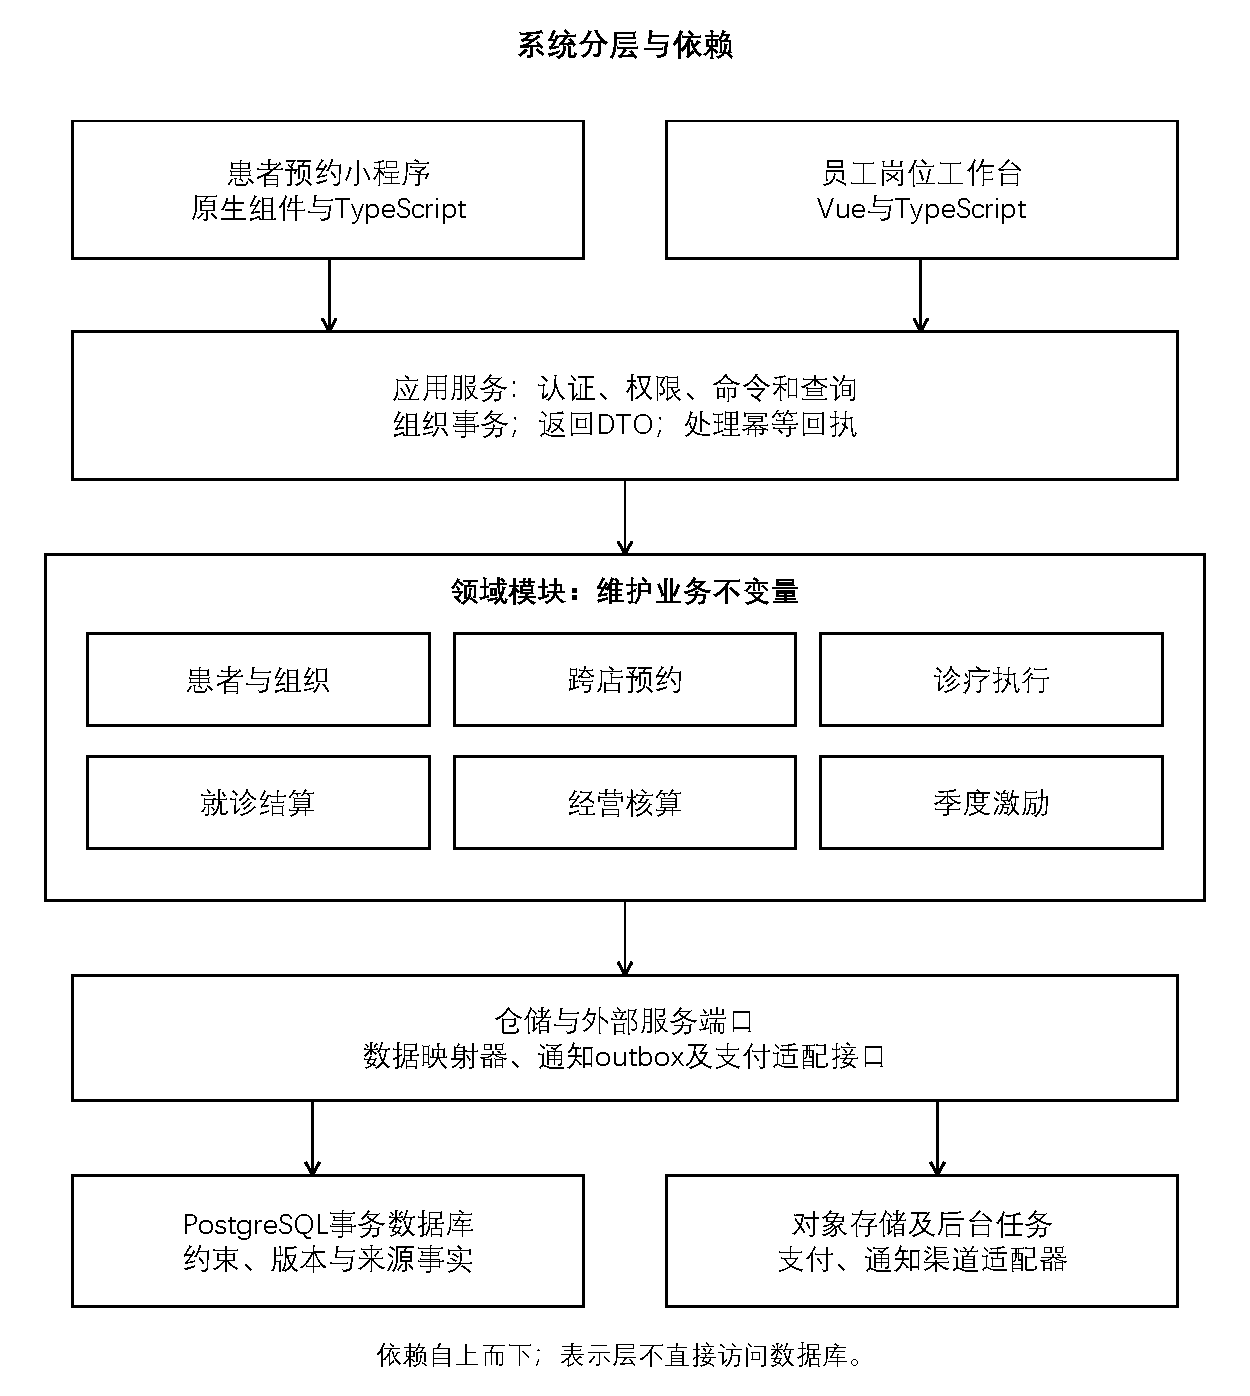
\includegraphics[width=\textwidth]{figures/architecture.pdf}
\caption{系统分层与依赖}\label{architecture}\end{figure}
\par\noindent\begin{minipage}{\textwidth}
{\fontsize{10.5pt}{13.2pt}\selectfont\setlength{\tabcolsep}{0pt}\renewcommand{\arraystretch}{1.08}
\captionof{table}{分层架构}\label{tab701}
\begin{tabular}{@{}p{2.540cm}@{\hspace{0.16cm}}p{8.240cm}@{\hspace{0.16cm}}p{4.340cm}@{}}
\toprule
\bfseries \Cell{层} & \bfseries \Cell{职责与技术选择} & \bfseries \Cell{依赖方向}\\\midrule
\Cell{患者表示层} & \Cell{微信原生小程序与Type\allowbreak{}Script，结合Vant Weapp组件组织预约、就诊人和复诊入口} & \Cell{通过HTTPS调用公开应用接口，不直连数据库。}\\[1pt]
\Cell{员工表示层} & \Cell{Vue 3、Type\allowbreak{}Script与Element Plus组件化后台；按前台、医生、店长和总部授权呈现工作台} & \Cell{页面调用独立API模块，表单状态与业务数据分开。}\\[1pt]
\Cell{应用层} & \Cell{Node.\allowbreak{}js与Type\allowbreak{}Script模块化服务，使用Fastify组织HTTP接口、认证、命令和查询} & \Cell{调用领域服务与仓储接口，不把校验复制到每个页面。}\\[1pt]
\Cell{领域层} & \Cell{患者、预约、诊疗、结算、季度核算六个业务模块} & \Cell{领域对象维护不变量，跨聚合规则由领域服务协调。}\\[1pt]
\Cell{基础设施层} & \Cell{Postgre\allowbreak{}SQL、数据映射器、对象存储、异步任务和外部渠道适配器} & \Cell{实现仓储及消息端口，外部细节不渗入领域规则。}\\[1pt]
\bottomrule\end{tabular}
}\end{minipage}\par\vspace{6pt}
15家门诊到约30家的目标适合先采用模块化单体和统一事务数据库。按业务边界组织代码与数据访问接口，可以保留清晰的职责而不引入分布式事务负担。通知和报表导出通过后台任务处理；缓存仅用于可重建的读取结果，预约可用性及资金余额最终以事务数据库为准。\par
\Needspace{378pt}
\subsection{领域边界与事务}
\par\noindent\begin{minipage}{\textwidth}
{\fontsize{10.5pt}{13.2pt}\selectfont\setlength{\tabcolsep}{0pt}\renewcommand{\arraystretch}{1.08}
\captionof{table}{聚合与跨模块联系}\label{tab704}
\begin{tabular}{@{}p{2.640cm}@{\hspace{0.16cm}}p{7.340cm}@{\hspace{0.16cm}}p{5.140cm}@{}}
\toprule
\bfseries \Cell{领域} & \bfseries \Cell{聚合根与主要不变量} & \bfseries \Cell{跨模块交接}\\\midrule
\Cell{身份与组织} & \Cell{患者、员工、门诊；稳定身份、资格与授权范围} & \Cell{向预约和诊疗提供所需身份及能力，不暴露无关人事信息。}\\[1pt]
\Cell{预约} & \Cell{预约及资源预留；医生与牙椅不得冲突} & \Cell{确认事件驱动提醒；到诊后建立就诊。}\\[1pt]
\Cell{诊疗} & \Cell{就诊、治疗计划、执行；确认先于新增执行，签署后追加附记} & \Cell{已签署执行为结算与用品成本提供来源。}\\[1pt]
\Cell{结算} & \Cell{唯一就诊单、收款、分配及退款；金额守恒和原单追溯} & \Cell{成功资金结果进入日结，服务收入进入经营核算。}\\[1pt]
\Cell{经营核算} & \Cell{成本来源、分摊和期间；来源不重复、归属可解释} & \Cell{关闭来源版本供医生季度结果使用。}\\[1pt]
\Cell{激励} & \Cell{季度结果、基金与个人分配；固定10\%基数及分配守恒} & \Cell{独立批准后才能登记发放，不承担工资代发。}\\[1pt]
\bottomrule\end{tabular}
}\end{minipage}\par\vspace{6pt}
{\fontsize{10.5pt}{13.2pt}\selectfont\setlength{\tabcolsep}{0pt}\renewcommand{\arraystretch}{1.08}
\begin{longtable}{@{}p{2.440cm}@{\hspace{0.16cm}}p{3.840cm}@{\hspace{0.16cm}}p{5.140cm}@{\hspace{0.16cm}}p{3.540cm}@{}}
\caption{关键事务与失败恢复}\label{tab705}\\
\toprule
\bfseries \Cell{操作} & \bfseries \Cell{受控范围} & \bfseries \Cell{锁与不变量} & \bfseries \Cell{失败恢复}\\\midrule
\endfirsthead
\toprule
\bfseries \Cell{操作} & \bfseries \Cell{受控范围} & \bfseries \Cell{锁与不变量} & \bfseries \Cell{失败恢复}\\\midrule
\endhead
\bottomrule\endlastfoot
\Cell{发布医生跨店班次} & \Cell{doctor\_\allowbreak{}shifts及审计} & \Cell{医生行；检查有效授权及资格，数据库排斥约束作为最后防线；同一医生全连锁有效班次不得时间重叠，区间按[开始,\allowbreak{}结束)\allowbreak{}处理} & \Cell{整体回滚，原班次及已约安排保持；资源变化另产生协调任务。}\\[1pt]
\Cell{号源占位与正式确认} & \Cell{booking\_\allowbreak{}holds、appointments、appointment\_\allowbreak{}events、notification\_\allowbreak{}tasks} & \Cell{按稳定编号顺序锁患者、医生、牙椅，再读班次、停用、占位及预约；统一处理已到期占位；患者、医生、牙椅不重叠；资源组一并承诺；确认时有效资格、窗口、时长与同意仍满足} & \Cell{不生成半个预约；占位到期后收到的付款保持真实预收并转人工处置，不反向抢占已给他人的号源。}\\[1pt]
\Cell{改约与候补补位} & \Cell{新旧预约、占位、事件及通知} & \Cell{旧预约版本及新旧医生牙椅，按统一顺序取得；新约创建与旧约标记rescheduled同事务；候补接受前不确认} & \Cell{新资源失败则保留旧约和资金归属；通知失败不回滚成功改约。}\\[1pt]
\Cell{医生签署实际治疗及计费} & \Cell{执行单、执行项目、临床记录、唯一Invoice及明细} & \Cell{就诊、适用方案版本及执行；唯一visit\_\allowbreak{}id与execution\_\allowbreak{}item\_\allowbreak{}id限制重复；患者、就诊、牙位、资格和同意一致；费用仅来自实际完成数量；一就诊一个Invoice身份} & \Cell{缺临床条件不签署；重复请求返回同一已存在单据，数据库冲突不产生第二张账。}\\[1pt]
\Cell{部分付款及跨店核销} & \Cell{成功收款、payment\_\allowbreak{}allocations及审计} & \Cell{原款、涉及Invoice按编号排序；重算成功退款和已批准冻结；净核销不超净原款和净应收；患者一致，跨店具备授权且保留往来来源} & \Cell{金额或范围不符整批回滚，既有核销和预收不被覆盖。}\\[1pt]
\Cell{费用减免与退款} & \Cell{费用调整独立提交；退款批准与实际执行分别提交} & \Cell{调整锁Invoice；批准锁原款及原核销；成功回执锁申请、退付和需释放的核销；获批冻结及成功未决退付不超来源；退款成功与核销释放原子完成；费用调整不改变现金事实} & \Cell{外部失败或未知保留待查，不能重发新交易或假记成功；拒绝审批不改变原款。}\\[1pt]
\Cell{实际材料成本归属} & \Cell{材料批次、耗用与冲回行} & \Cell{来源批次及原耗用行；数量和分值不超来源，最后一份承担尾差；一笔用品不再次进入运营费用} & \Cell{不足、隔离或证据不全不确认耗用；更正追加反向行不覆盖原记录。}\\[1pt]
\Cell{运营费分摊} & \Cell{费用凭据及全部cost\_\allowbreak{}allocations} & \Cell{费用凭据、核验工时快照；审批按自然员工分离；直接归属有明确医生；共享以真实核验工时为动因；分配合计等于来源分值} & \Cell{零分母、重复凭据或金额不守恒时拒绝批准，不保存部分已批准分配。}\\[1pt]
\Cell{跨店内部清算} & \Cell{清算单、来源分配和外部事件} & \Cell{按门诊对及来源核销编号锁定未清余额；成功和未决指令不超未清来源；只有核实成功才减少内部往来} & \Cell{银行未知保留预占并查询原指令；失败释放，不新增患者收入。}\\[1pt]
\Cell{月度关账与迟到更正} & \Cell{period\_\allowbreak{}closes及来源快照} & \Cell{门诊月份控制行；资金、计费、材料和费用写入先检查该月份锁；关账来源集合稳定且月份唯一有效；正常应收预收可结转} & \Cell{预检失败保持开放；普通迟到更正进当前开放月并引用原日期。重大重开需独立批准、新版本和受影响季度重算，不静默改旧利润。}\\[1pt]
\Cell{季度业绩及10\%激励} & \Cell{医生门诊结果、逐笔来源、全链基金、来源及分配} & \Cell{季度计算批次；固定全部三个月有效关账及全范围来源版本；先合计医生门诊正负净利；池额round(\allowbreak{}max(\allowbreak{}0,\allowbreak{}总净利)\allowbreak{}*\allowbreak{}10\%)\allowbreak{}；跨店合并医生正贡献形成权重；分配总额等于池额} & \Cell{缺月、漏亏损来源、来源变动或尾差不守恒时不批准；建立新版本而非覆盖已批准结果。}\\[1pt]
\Cell{激励实际发放} & \Cell{incentive\_\allowbreak{}payments及获批份额} & \Cell{医生同季度的有效分配版本及历史成功、在途发放；累计成功及未决不超当前有效获批份额；新版本先扣原已付和在途，不重新支付全额} & \Cell{未知查询原指令，失败释放；成功付款记录不可因分配重编而删除。}\\[1pt]
\Cell{写命令回执和通知outbox} & \Cell{command\_\allowbreak{}receipts、用例聚合、audit\_\allowbreak{}events及notification\_\allowbreak{}tasks/\allowbreak{}资金发件事件} & \Cell{先认证和授权，按actor\_\allowbreak{}key/\allowbreak{}request\_\allowbreak{}id取得唯一命令；随后按用例的固定聚合顺序加锁；业务变更、最终命令决策和待发任务一次提交；同键不同内容拒绝，重复同内容只重放原决策} & \Cell{提交前崩溃整体回滚；已提交响应丢失重放回执。外部调用在事务外，由租约、重试、验真回执与人工未知队列恢复，不将外部成功宣称为本地原子操作。}\\[1pt]
\Cell{预约意向与资源承诺衔接} & \Cell{appointment\_\allowbreak{}requests、候补及最终预约} & \Cell{申请及其有效候补；确认资源仍按固定患者医生牙椅顺序锁定；申请和邀约不占作正式承诺；同意图满足后同步关联最终预约，需求统计沿来源去重} & \Cell{未匹配保留待处理状态，不生成虚假预约；资源失败不丢原意向。}\\[1pt]
\end{longtable}
}
Postgre\allowbreak{}SQL时间范围与排斥约束用于同一资源区间冲突，数据库唯一约束保证一就诊一单。普通CHECK不能可靠维护跨行合计，款项分配、成本分摊和激励额度由受锁事务中的领域校验维护；对高冲突操作采用行锁或可串行化事务并处理重试。事务失败向调用者返回业务冲突，不能把异常吞掉后返回成功。[R8]\par
\Needspace{412pt}
\subsection{公共接口契约}
\par\noindent\begin{minipage}{\textwidth}
{\fontsize{10.5pt}{13.2pt}\selectfont\setlength{\tabcolsep}{0pt}\renewcommand{\arraystretch}{1.08}
\captionof{table}{接口公共约定}\label{tab708}
\begin{tabular}{@{}p{2.940cm}@{\hspace{0.16cm}}p{12.340cm}@{}}
\toprule
\bfseries \Cell{内容} & \bfseries \Cell{设计}\\\midrule
\Cell{命令标识} & \Cell{预约确认、取消和改期请求携带 Idempotency-\allowbreak{}Key；同一身份、同一键及相同请求返回原结果，内容不同时拒绝。需防止覆盖的更新提交 expected\allowbreak{}Version 或 hold\allowbreak{}Version。}\\[1pt]
\Cell{权限} & \Cell{服务端从会话解析患者身份、员工角色和门诊范围；患者访问本人预约，员工按岗位授权办理，并记录实际操作者和就诊人。}\\[1pt]
\Cell{错误结构} & \Cell{成功响应包含 data 和 request\allowbreak{}Id；错误响应包含 error.\allowbreak{}code、error.\allowbreak{}message、可选 details 和 request\allowbreak{}Id，区分权限、资料、资源冲突和状态错误。}\\[1pt]
\Cell{分页} & \Cell{患者与员工预约列表按 page、page\allowbreak{}Size 查询，返回 items、total、page 和 page\allowbreak{}Size；按稳定条件筛选并明确当前查询范围。}\\[1pt]
\Cell{异步回调} & \Cell{验证渠道签名、金额、币种、商户和原交易关系；重复事件按唯一事件号去重，乱序结果按合法状态处理。}\\[1pt]
\Cell{日志} & \Cell{记录操作及业务标识，不记录密码、完整支付凭证或不必要的敏感病史。审计与可观测日志职责分开。}\\[1pt]
\bottomrule\end{tabular}
}\end{minipage}\par\vspace{6pt}
{\fontsize{10.5pt}{13.2pt}\selectfont\setlength{\tabcolsep}{0pt}\renewcommand{\arraystretch}{1.08}
\begin{longtable}{@{}p{2.140cm}@{\hspace{0.16cm}}p{13.140cm}@{}}
\caption{用例到接口的追踪}\label{tab709}\\
\toprule
\bfseries \Cell{用例} & \bfseries \Cell{接口设计}\\\midrule
\endfirsthead
\toprule
\bfseries \Cell{用例} & \bfseries \Cell{接口设计}\\\midrule
\endhead
\bottomrule\endlastfoot
\Cell{\mbox{UC-01}} & \Cell{POST /\allowbreak{}auth/\allowbreak{}register 建立患者账号与资料；GET、PUT /\allowbreak{}patients/\allowbreak{}me 读取和更新本人资料，更新携带 expected\allowbreak{}Version；前台通过 GET、POST /\allowbreak{}staff/\allowbreak{}patients 核对或建档。}\\[1pt]
\Cell{\mbox{UC-02}} & \Cell{GET /\allowbreak{}doctors、GET /\allowbreak{}qualifications 查询医生与资格；POST、PUT /\allowbreak{}staff/\allowbreak{}doctors 和 /\allowbreak{}staff/\allowbreak{}qualifications 维护授权范围内的医生与资格资料。}\\[1pt]
\Cell{\mbox{UC-03}} & \Cell{GET /\allowbreak{}services 查询服务；POST、PUT /\allowbreak{}staff/\allowbreak{}services 维护项目、时长与资格要求；GET /\allowbreak{}treatment-\allowbreak{}references 提供独立的治疗参考价。}\\[1pt]
\Cell{\mbox{UC-04}} & \Cell{GET /\allowbreak{}shifts 查询排班；POST /\allowbreak{}staff/\allowbreak{}shifts 发布班次，POST /\allowbreak{}staff/\allowbreak{}shifts/\allowbreak{}\{id\}/\allowbreak{}cancel 撤销班次。服务端校验门诊授权、资格、跨店时间及转场。}\\[1pt]
\Cell{\mbox{UC-05}} & \Cell{GET /\allowbreak{}booking-\allowbreak{}policy 返回规则与日期查询范围；GET /\allowbreak{}booking-\allowbreak{}slots 按 clinic\allowbreak{}Id、service\allowbreak{}Id、date 及可选 doctor\allowbreak{}Id 查询候选时段。}\\[1pt]
\Cell{\mbox{UC-06}} & \Cell{POST /\allowbreak{}booking-\allowbreak{}holds 取得临时占位；POST /\allowbreak{}appointments/\allowbreak{}confirm 携带 hold\allowbreak{}Id、hold\allowbreak{}Version 和 Idempotency-\allowbreak{}Key 确认；GET /\allowbreak{}appointments/\allowbreak{}\{id\} 查询结果。}\\[1pt]
\Cell{\mbox{UC-07}} & \Cell{改期先通过 POST /\allowbreak{}booking-\allowbreak{}holds 取得新占位；POST /\allowbreak{}appointments/\allowbreak{}\{id\}/\allowbreak{}changes 携带 intent、reason、expected\allowbreak{}Version 和 Idempotency-\allowbreak{}Key，改期另传 hold\allowbreak{}Id、hold\allowbreak{}Version。}\\[1pt]
\Cell{\mbox{UC-08}} & \Cell{POST /\allowbreak{}contact-\allowbreak{}tasks；POST /\allowbreak{}waitlist-\allowbreak{}invitations/\allowbreak{}\{id\}/\allowbreak{}responses；回执入口校验来源与事件唯一号。}\\[1pt]
\Cell{\mbox{UC-09}} & \Cell{POST /\allowbreak{}appointments/\allowbreak{}\{id\}/\allowbreak{}attendance；POST /\allowbreak{}attendance-\allowbreak{}events/\allowbreak{}\{id\}/\allowbreak{}corrections。更正带证据、理由与版本。}\\[1pt]
\Cell{\mbox{UC-10}} & \Cell{POST /\allowbreak{}visits/\allowbreak{}\{id\}/\allowbreak{}assessments；POST /\allowbreak{}treatment-\allowbreak{}plans；POST /\allowbreak{}treatment-\allowbreak{}plans/\allowbreak{}\{id\}/\allowbreak{}versions。签署人由会话及资格确定。}\\[1pt]
\Cell{\mbox{UC-11}} & \Cell{GET /\allowbreak{}plan-\allowbreak{}versions/\allowbreak{}\{id\}/\allowbreak{}explanation；POST /\allowbreak{}plan-\allowbreak{}versions/\allowbreak{}\{id\}/\allowbreak{}consents，带scope、decision、evidence\allowbreak{}Ref及幂等键。}\\[1pt]
\Cell{\mbox{UC-12}} & \Cell{POST /\allowbreak{}visits/\allowbreak{}\{id\}/\allowbreak{}executions；POST /\allowbreak{}executions/\allowbreak{}\{id\}/\allowbreak{}signatures；POST /\allowbreak{}executions/\allowbreak{}\{id\}/\allowbreak{}addenda。签署校验医生本人及版本。}\\[1pt]
\Cell{\mbox{UC-13}} & \Cell{POST /\allowbreak{}visits/\allowbreak{}\{visit\allowbreak{}Id\}/\allowbreak{}record/\allowbreak{}sign；POST /\allowbreak{}signed-\allowbreak{}records/\allowbreak{}\{id\}/\allowbreak{}addenda。}\\[1pt]
\Cell{\mbox{UC-14}} & \Cell{POST /\allowbreak{}stage-\allowbreak{}tasks/\allowbreak{}\{id\}/\allowbreak{}appointments；POST /\allowbreak{}handovers/\allowbreak{}\{id\}/\allowbreak{}decision。}\\[1pt]
\Cell{\mbox{UC-15}} & \Cell{POST /\allowbreak{}visits/\allowbreak{}\{visit\allowbreak{}Id\}/\allowbreak{}invoice/\allowbreak{}prepare；GET /\allowbreak{}visits/\allowbreak{}\{visit\allowbreak{}Id\}/\allowbreak{}invoice。}\\[1pt]
\Cell{\mbox{UC-16}} & \Cell{POST /\allowbreak{}receipts；POST /\allowbreak{}receipts/\allowbreak{}\{id\}/\allowbreak{}confirm；POST /\allowbreak{}receipts/\allowbreak{}\{id\}/\allowbreak{}allocations。}\\[1pt]
\Cell{\mbox{UC-17}} & \Cell{POST /\allowbreak{}corrections；POST /\allowbreak{}corrections/\allowbreak{}\{id\}/\allowbreak{}approval；POST /\allowbreak{}refunds/\allowbreak{}\{id\}/\allowbreak{}verified-\allowbreak{}result。}\\[1pt]
\Cell{\mbox{UC-18}} & \Cell{POST /\allowbreak{}daily-\allowbreak{}closes/\allowbreak{}prepare；POST /\allowbreak{}daily-\allowbreak{}closes/\allowbreak{}\{id\}/\allowbreak{}review；POST /\allowbreak{}interclinic-\allowbreak{}items/\allowbreak{}\{id\}/\allowbreak{}confirm。}\\[1pt]
\Cell{\mbox{UC-19}} & \Cell{POST /\allowbreak{}period-\allowbreak{}costs；POST /\allowbreak{}period-\allowbreak{}costs/\allowbreak{}\{id\}/\allowbreak{}allocations；POST /\allowbreak{}cost-\allowbreak{}allocations/\allowbreak{}\{id\}/\allowbreak{}review。}\\[1pt]
\Cell{\mbox{UC-20}} & \Cell{POST /\allowbreak{}periods/\allowbreak{}\{id\}/\allowbreak{}closing-\allowbreak{}package；POST /\allowbreak{}closing-\allowbreak{}packages/\allowbreak{}\{id\}/\allowbreak{}close。}\\[1pt]
\Cell{\mbox{UC-21}} & \Cell{POST /\allowbreak{}quarters/\allowbreak{}\{id\}/\allowbreak{}performance-\allowbreak{}trials；GET /\allowbreak{}performance-\allowbreak{}trials/\allowbreak{}\{id\}/\allowbreak{}sources。}\\[1pt]
\Cell{\mbox{UC-22}} & \Cell{POST /\allowbreak{}performance-\allowbreak{}trials/\allowbreak{}\{id\}/\allowbreak{}distribution-\allowbreak{}review；POST /\allowbreak{}incentive-\allowbreak{}shares/\allowbreak{}\{id\}/\allowbreak{}payouts。}\\[1pt]
\Cell{\mbox{UC-23}} & \Cell{GET /\allowbreak{}reports/\allowbreak{}appointment-\allowbreak{}skill-\allowbreak{}demand；POST /\allowbreak{}reports/\allowbreak{}\{id\}/\allowbreak{}management-\allowbreak{}actions。}\\[1pt]
\Cell{\mbox{UC-24}} & \Cell{POST /\allowbreak{}assignments；POST /\allowbreak{}assignments/\allowbreak{}\{id\}/\allowbreak{}revoke；POST /\allowbreak{}staff/\allowbreak{}\{id\}/\allowbreak{}deactivation。}\\[1pt]
\end{longtable}
}
\Needspace{483pt}
\subsection{患者小程序}
\begin{figure}[H]\centering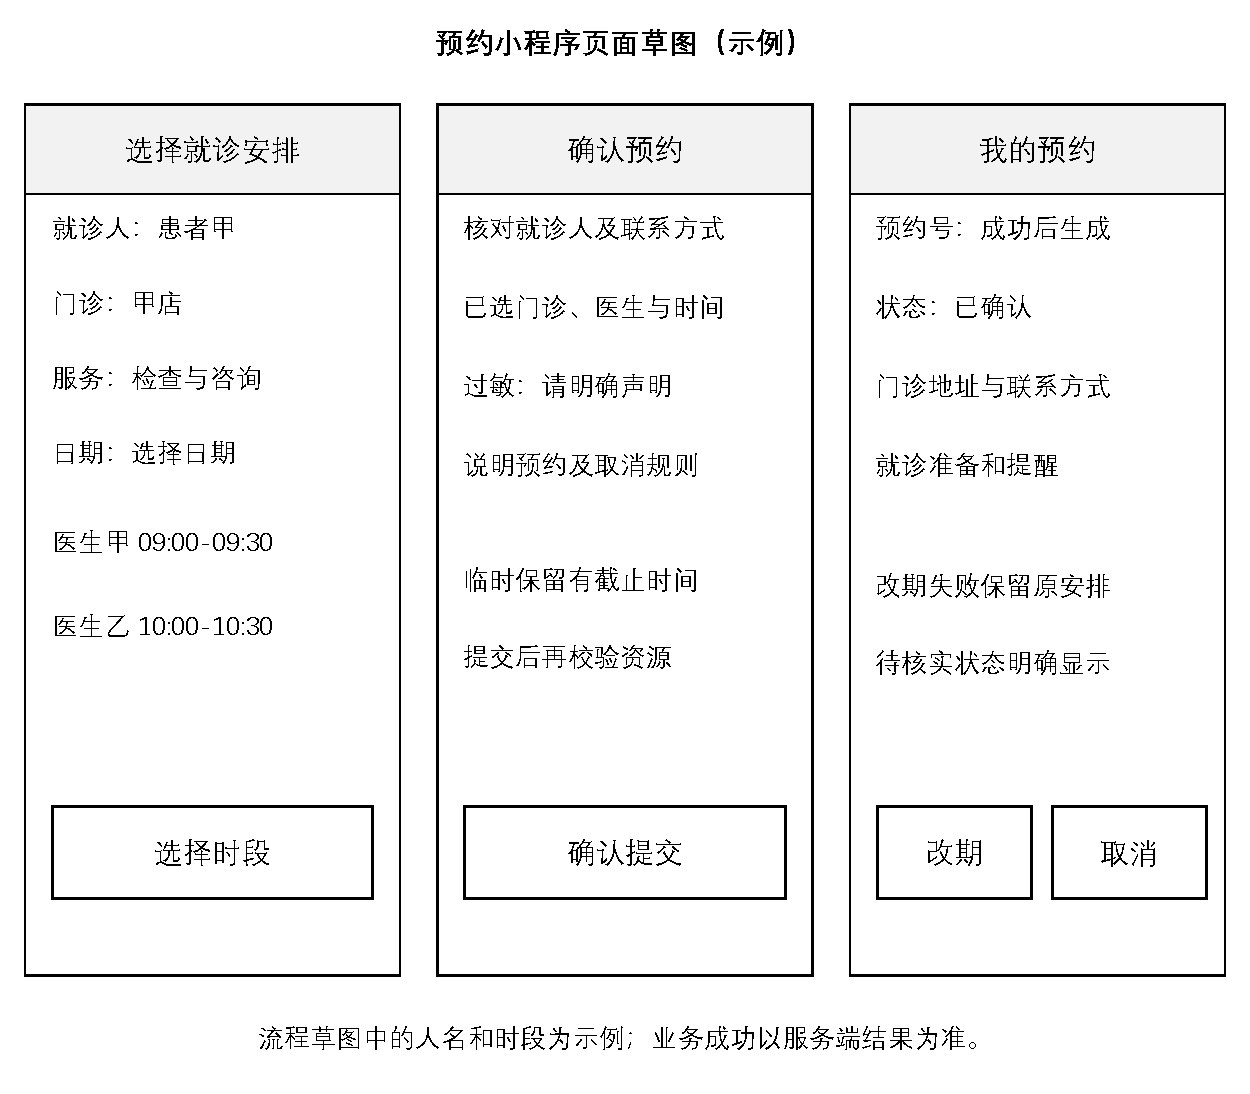
\includegraphics[width=\textwidth]{figures/booking_wireframe.pdf}
\caption{预约小程序页面草图（示例）}\label{booking_wireframe}\end{figure}
\par\noindent\begin{minipage}{\textwidth}
{\fontsize{10.5pt}{13.2pt}\selectfont\setlength{\tabcolsep}{0pt}\renewcommand{\arraystretch}{1.08}
\captionof{table}{患者页面及交互}\label{tab712}
\begin{tabular}{@{}p{3.040cm}@{\hspace{0.16cm}}p{6.840cm}@{\hspace{0.16cm}}p{5.240cm}@{}}
\toprule
\bfseries \Cell{页面} & \bfseries \Cell{主要信息与动作} & \bfseries \Cell{异常或等待状态}\\\midrule
\Cell{首页与门诊选择} & \Cell{展示地址、联系方式和可预约服务，选择患者及日期} & \Cell{尚未建档时引导补资料，不能默认账号本人就是就诊人。}\\[1pt]
\Cell{号源与确认} & \Cell{展示门诊、医生、时长及可约时段，说明临时保留和最终确认区别} & \Cell{占位到期或竞争失败保留输入，提供替代时段或前台联系。}\\[1pt]
\Cell{我的预约} & \Cell{查看安排、准备事项、取消及改期入口} & \Cell{未确认申请、已取消、已改期和已到诊使用不同提示。}\\[1pt]
\Cell{治疗方案与费用} & \Cell{查看医生解释、方案版本、增项及当次结算明细} & \Cell{未确认不能呈现为已执行；费用异议提供原单申请入口。}\\[1pt]
\Cell{付款与退款} & \Cell{显示原交易、已分配、欠款及退款处理状态} & \Cell{支付回跳后仍向服务端查询，未知状态提示处理中并避免再次扣款。}\\[1pt]
\Cell{复诊与资料} & \Cell{维护就诊人、逐项过敏、复诊任务及跨店授权} & \Cell{更改健康资料提示医生复核，授权可以按范围和用途管理。}\\[1pt]
\bottomrule\end{tabular}
}\end{minipage}\par\vspace{6pt}
患者预约页面按门诊、服务、日期和医生组织筛选，提供七日快捷日期和弹出日历。可查询日期范围由预约策略统一返回，选择日期后再请求实际号源；页面按门诊当地时间将返回时段归入上午、下午和晚间，并保留时段对应的医生、牙椅、班次和起止信息。日期可选后还需查询实际号源；选择时段后通过服务端短时占位保留资源。\par
号源页分别呈现加载中、查询失败和查询成功但无匹配时段的状态，查询失败可重试。患者改变筛选条件或离开页面后，过期响应不得覆盖当前结果。预约确认、取消和改期均以服务端返回的结果更新页面；网络中断导致结果未明时，保留原操作标识并核对结果，避免再次提交产生重复预约。\par
患者可浏览医生介绍、擅长方向和可预约的咨询服务，并按项目类别查看价格参考区间、单位、年份及资料来源。参考区间用于就诊前了解费用，具体诊疗方案和实际费用经面诊确认；种植、正畸等复杂项目可先预约评估或咨询，不把参考疗程价格作为一次预约收费。\par
\Needspace{338pt}
\subsection{员工工作台与组件}
\par\noindent\begin{minipage}{\textwidth}
{\fontsize{10.5pt}{13.2pt}\selectfont\setlength{\tabcolsep}{0pt}\renewcommand{\arraystretch}{1.08}
\captionof{table}{工作台与可复用组件}\label{tab717}
\begin{tabular}{@{}p{2.840cm}@{\hspace{0.16cm}}p{6.140cm}@{\hspace{0.16cm}}p{6.140cm}@{}}
\toprule
\bfseries \Cell{对象} & \bfseries \Cell{组成} & \bfseries \Cell{职责}\\\midrule
\Cell{前台} & \Cell{日历、候诊队列、待收费、日结和通知待办} & \Cell{预约列表分页，成功动作局部刷新，未保存编辑有离开提示。}\\[1pt]
\Cell{医生} & \Cell{今日接诊、风险摘要、计划版本、执行行和签署} & \Cell{牙位与单位输入独立组件；签署前检查新增项目确认和用品耗用。}\\[1pt]
\Cell{店长} & \Cell{班次冲突、门诊容量、日结差异和成本来源} & \Cell{批量变更先预览影响，不允许静默取消其他店预约。}\\[1pt]
\Cell{总部} & \Cell{资格及组织、跨店代收、期间复核、医生季度结果和基金} & \Cell{每个汇总可下钻来源，制表与复核任务分开。}\\[1pt]
\Cell{共享组件} & \Cell{患者选择、单位金额、状态标签、时间范围、证据附件与版本冲突提示} & \Cell{组件只处理表示逻辑，最终业务校验由服务端执行。}\\[1pt]
\bottomrule\end{tabular}
}\end{minipage}\par\vspace{6pt}
前端按患者、预约、诊疗、结算和经营模块组织，API调用、缓存查询、表单草稿和页面组件分层。避免一个入口文件包办所有业务。权限菜单只改善使用体验，服务端仍需逐请求校验；任何页面隐藏都不能替代权限控制。\par
预约与排班工作区提供前一天、今天、后一天及七日日期导航。员工可在预约列表与按医生分组的单日日程之间切换，排班可按医生卡片查看；医生工作区以本人预约和排班为中心，其他岗位按机构与岗位授权查看相应范围。选中日期及门诊变化时重新查询，窄屏可横向浏览日期与展开导航；页面处于可见状态时定期刷新预约，显示最新改期或取消结果。\par
按医生分组的日程按页获取选定日期的预约，并检查总数、重复记录及首批数据版本。查询期间数据变化或记录未完整加载时提示重新查询，不能将当前页当作完整日程。排班卡片标明查询范围和数量限制，不能将查询结果数量直接解释为可预约容量。\par
资源维护页按范围筛选医生、门诊及牙椅，展示医生资格生效和失效日期，并区分未生效、生效中和已过期。资格标签服务于管理判断，发布班次和确认预约时仍由服务端核验资格是否覆盖整个服务区间。页面在筛选或账号变更后舍弃旧响应，以免过期结果覆盖当前资料。\par
\Needspace{208pt}
\section{质量要求与验收设计}
{\fontsize{10.5pt}{13.2pt}\selectfont\setlength{\tabcolsep}{0pt}\renewcommand{\arraystretch}{1.08}
\begin{longtable}{@{}p{1.440cm}@{\hspace{0.16cm}}p{2.940cm}@{\hspace{0.16cm}}p{10.740cm}@{}}
\caption{全局业务规则}\label{tab723}\\
\toprule
\bfseries \Cell{编号} & \bfseries \Cell{主题} & \bfseries \Cell{不变量与处理}\\\midrule
\endfirsthead
\toprule
\bfseries \Cell{编号} & \bfseries \Cell{主题} & \bfseries \Cell{不变量与处理}\\\midrule
\endhead
\bottomrule\endlastfoot
\Cell{\mbox{BR01}} & \Cell{患者唯一身份} & \Cell{同一患者跨门诊沿用稳定标识；手机号可以由家庭共用，不能单独作为患者唯一键。疑似重复先核对，不自动合并。}\\[1pt]
\Cell{\mbox{BR02}} & \Cell{过敏核对} & \Cell{过敏目录与患者为多对多。known必须有有效明细；unknown不能当作none\_\allowbreak{}reported。医生接诊重新核对并记录结果。}\\[1pt]
\Cell{\mbox{BR03}} & \Cell{资格与排班} & \Cell{服务所需资格必须在整个服务区间有效。医生在全连锁的有效班次和预约不得重叠；跨店连续班次保留明确转场间隔。}\\[1pt]
\Cell{\mbox{BR04}} & \Cell{资源承诺} & \Cell{可预约容量由已发布班次、服务时长和牙椅共同确定。查询不占位；确认在事务内复核，冲突时不能返回成功。}\\[1pt]
\Cell{\mbox{BR05}} & \Cell{改期与取消} & \Cell{改期先取得新资源再原子释放旧资源。取消保留原安排和原因；取消与退款不是同一状态变化。}\\[1pt]
\Cell{\mbox{BR06}} & \Cell{出席事实} & \Cell{attended初始false，仅由实际到诊事件置true。取消、改期、未来待到和确认未到分别记录，false不能推导具体原因。}\\[1pt]
\Cell{\mbox{BR07}} & \Cell{计划与增项} & \Cell{意向不是已实施治疗。方案确认锁定版本与费用边界；治疗增项在执行前取得患者确认，保留同意证据。}\\[1pt]
\Cell{\mbox{BR08}} & \Cell{执行与计价} & \Cell{实际执行记录包含就诊、医生、治疗项目、标准单位、数量及适用单价快照。停止使用的目录项不改变历史记录。}\\[1pt]
\Cell{\mbox{BR09}} & \Cell{单次就诊结算} & \Cell{每次就诊最多一个稳定Invoice身份，正式结算前必须生成该单；一张单只属于一次就诊，明细只能来自该次实际治疗。}\\[1pt]
\Cell{\mbox{BR10}} & \Cell{收款与收入} & \Cell{治疗收入按已签署且已出具结算单的服务事实及关联调整归属，结算单已出具不要求已收清；收款按成功交易统计。预收和内部转款不能重复计入治疗收入。}\\[1pt]
\Cell{\mbox{BR11}} & \Cell{金额守恒} & \Cell{金额以人民币分存储；数量为定点小数。逐行按数量乘单价四舍五入到分，再汇总；收款分配、费用分摊和激励分配各自守恒。}\\[1pt]
\Cell{\mbox{BR12}} & \Cell{退款边界} & \Cell{费用减免用调整单减少应收；退款用关联原收款的实际负向资金事件。退钱本身不再重复扣减收入，退款金额不得超过可退余额。}\\[1pt]
\Cell{\mbox{BR13}} & \Cell{成本归属} & \Cell{医疗用品按执行耗用与成本快照归属实际医生。运营费用先直接归属，无法直接归属的共同费用按已复核动因分摊，同一来源不可重复计入。}\\[1pt]
\Cell{\mbox{BR14}} & \Cell{关账顺序} & \Cell{先核验执行与结算完整性、收退款及代收差异，再复核成本，最后关闭期间。未解决差异阻止关账；事后调整关联原事实并计入获准开放期间。}\\[1pt]
\Cell{\mbox{BR15}} & \Cell{季度净利润} & \Cell{每医生季度净利润=\allowbreak{}治疗收入净额-医疗用品成本-医生运营费用；跨店合并保留门诊来源，负贡献不得删除。}\\[1pt]
\Cell{\mbox{BR16}} & \Cell{基金提取} & \Cell{季度基金=\allowbreak{}四舍五入到分[max(\allowbreak{}0,\allowbreak{}全体医生季度净利润合计)\allowbreak{}×10\%]。先合计含负值的利润，再判定是否提取；10\%为固定提取比例。}\\[1pt]
\Cell{\mbox{BR17}} & \Cell{个人分配} & \Cell{个人分配采用正净贡献占比；负贡献医生当期分配为0，仍参与基金总基数。按最大余数法分配尾差，合计必须等于获批基金；股权比例不作为分配权重。}\\[1pt]
\Cell{\mbox{BR18}} & \Cell{职责分离} & \Cell{费用更正、退款、关账和激励分配的提交人与复核人必须不同。总部按岗位任务授权，店长不能凭运营角色签署病历。}\\[1pt]
\Cell{\mbox{BR19}} & \Cell{审计与消息} & \Cell{状态变化记录操作者、业务时间、原因及前后版本。业务提交与待发通知同事务保存，通知失败产生重试和人工待办，不能撤销已确认业务。}\\[1pt]
\end{longtable}
}
\par\noindent\begin{minipage}{\textwidth}
{\fontsize{10.5pt}{13.2pt}\selectfont\setlength{\tabcolsep}{0pt}\renewcommand{\arraystretch}{1.08}
\captionof{table}{质量目标与验证条件}\label{tab724}
\begin{tabular}{@{}p{1.540cm}@{\hspace{0.16cm}}p{2.840cm}@{\hspace{0.16cm}}p{10.740cm}@{}}
\toprule
\bfseries \Cell{编号} & \bfseries \Cell{要求} & \bfseries \Cell{验证方式与通过条件}\\\midrule
\Cell{\mbox{QR01}} & \Cell{可用性} & \Cell{前台和患者分别走查预约、改期和付款异常；关键状态及恢复动作可见，不因错误丢失已填资料。}\\[1pt]
\Cell{\mbox{QR02}} & \Cell{并发一致性} & \Cell{两个请求同时争用一时段；仅一个确认，另一个可重新选择。收款、退款和分配并发不得超额。}\\[1pt]
\Cell{\mbox{QR03}} & \Cell{性能} & \Cell{以30门诊、100万预约/\allowbreak{}就诊事实的固定生成数据，测试200并发查询；号源和患者历史查询P95目标≤2秒。记录硬件、索引、冷热缓存和失败率，结果未达标则定位查询及容量。}\\[1pt]
\Cell{\mbox{QR04}} & \Cell{可恢复性} & \Cell{数据库每日全量备份并保存可恢复的增量日志，演练目标RPO≤15分钟、RTO≤4小时；恢复后核对金额及关键关系。该数值是设计目标。}\\[1pt]
\Cell{\mbox{QR05}} & \Cell{权限与隐私} & \Cell{对患者互访、员工跨店及总部查询临床详情逐项否定测试；越权无数据返回且审计留痕。}\\[1pt]
\Cell{\mbox{QR06}} & \Cell{审计与维护} & \Cell{每笔受控变更可定位操作者、请求、版本与来源；按用例组织契约测试及变更评审。}\\[1pt]
\Cell{\mbox{QR07}} & \Cell{扩展性} & \Cell{增加门诊或资格目录不复制业务代码；跨店规则及报表使用统一门诊标识。}\\[1pt]
\Cell{\mbox{QR08}} & \Cell{资金与核算} & \Cell{所有金额守恒条件以分校验；关闭季度结果可从固定来源重算，含负贡献及尾差测试。}\\[1pt]
\bottomrule\end{tabular}
}\end{minipage}\par\vspace{6pt}
\Needspace{459pt}
\subsection{端到端业务验收}
\par\noindent\begin{minipage}{\textwidth}
{\fontsize{10.5pt}{13.2pt}\selectfont\setlength{\tabcolsep}{0pt}\renewcommand{\arraystretch}{1.08}
\captionof{table}{业务链验收场景}\label{tab726}
\begin{tabular}{@{}p{2.840cm}@{\hspace{0.16cm}}p{5.040cm}@{\hspace{0.16cm}}p{7.240cm}@{}}
\toprule
\bfseries \Cell{场景} & \bfseries \Cell{关键输入} & \bfseries \Cell{可观察的结果}\\\midrule
\Cell{电话与线上竞争} & \Cell{同一医生、门诊及牙椅时段的两个患者} & \Cell{只有一个预约确认；另一方明确失败且无孤立资源占用。}\\[1pt]
\Cell{跨店技能与时间} & \Cell{同一医生跨店班次、资格到期及转场间隔不足} & \Cell{冲突或资格不足不能发布；有效调整保留版本和受影响预约清单。}\\[1pt]
\Cell{增项到结算} & \Cell{原方案一项，诊疗中新增一项} & \Cell{先确认增项再执行，两项均保留单位和单价快照，只形成同次就诊一张单。}\\[1pt]
\Cell{部分收款与退款} & \Cell{500元费用支付300元，之后批准减免100元并按条件退款} & \Cell{应收调整和退款各记一次，现金与收入分别可核对，不重复冲减。}\\[1pt]
\Cell{跨店代收} & \Cell{甲店治疗，乙店成功收款} & \Cell{服务收入归甲店医生，资金归乙店核对，内部划转不增加患者收入。}\\[1pt]
\Cell{医生季度含亏损} & \Cell{净利润70000、40000、-15000元} & \Cell{总净利润95000元，基金9500元，分配合计9500元；不能算11000元基金。}\\[1pt]
\Cell{历史价格变更} & \Cell{开单后目录价格上调} & \Cell{历史执行和结算保持原单位价，季度重算不使用新价格。}\\[1pt]
\Cell{通知与支付中断} & \Cell{提交成功后通知失败，退款调用超时} & \Cell{预约不撤回；通知形成待办。退款保持待核实，查原交易后再决定重试。}\\[1pt]
\bottomrule\end{tabular}
}\end{minipage}\par\vspace{6pt}
\subsection{部署与维护方案}
部署采用HTTPS入口、应用服务、后台任务和独立数据库，区分开发、验收及正式环境。数据库只向服务端开放；配置、密钥和备份凭证由运行环境提供，不能写入前端包或文档样例。附件存储使用受限访问和短时授权，病历、过敏及支付凭据按业务权限读取。\par
数据库结构变更使用带版本、校验和与回退说明的迁移。发布前在备份副本验证迁移与恢复，核对外键、单据唯一性、金额守恒和季度来源版本；失败时停止切换并恢复上一可用环境。监控聚焦请求失败、任务积压、预约冲突率、在途支付时长及备份滞后，告警必须对应处理责任人。\par
验收按用例契约、数据库约束、并发场景和端到端链路执行。这里定义的是验证方案；只有记录实际环境、输入和结果，才能判定目标是否达到。内部模型的一致性检查不能代替真实业务人员的走查或运行环境验收。\par
\Needspace{459pt}
\subsection{需求与设计追踪}
\par\noindent\begin{minipage}{\textwidth}
{\fontsize{10.5pt}{13.2pt}\selectfont\setlength{\tabcolsep}{0pt}\renewcommand{\arraystretch}{1.08}
\captionof{table}{核心业务需求的实现链}\label{tab732}
\begin{tabular}{@{}p{3.440cm}@{\hspace{0.16cm}}p{2.840cm}@{\hspace{0.16cm}}p{3.140cm}@{\hspace{0.16cm}}p{5.540cm}@{}}
\toprule
\bfseries \Cell{需求} & \bfseries \Cell{业务过程} & \bfseries \Cell{系统用例} & \bfseries \Cell{关键数据与验收}\\\midrule
\Cell{患者与多项过敏} & \Cell{\mbox{AS01}、\mbox{BP02}、\mbox{BP04}} & \Cell{\mbox{UC-01}、\mbox{UC-10}} & \Cell{患者及过敏关联；未知不当作无过敏。}\\[1pt]
\Cell{医生资格及跨店服务} & \Cell{\mbox{AS01}、\mbox{BP01}、\mbox{BP07}} & \Cell{\mbox{UC-02}、\mbox{UC-04}、\mbox{UC-05}、\mbox{UC-14}} & \Cell{资格多对多、班次与交接；全局冲突校验。}\\[1pt]
\Cell{电话预约升级} & \Cell{\mbox{AS01}、\mbox{BP02}、\mbox{BP03}} & \Cell{\mbox{UC-05}至\mbox{UC-09}} & \Cell{自助与代约同源；取消、改期和未到分别记录。}\\[1pt]
\Cell{多治疗、增项及单位价} & \Cell{\mbox{AS02}、\mbox{BP04}、\mbox{BP05}} & \Cell{\mbox{UC-03}、\mbox{UC-10}至\mbox{UC-13}} & \Cell{计划、同意及执行；保存标准单位、数量和单价快照。}\\[1pt]
\Cell{一就诊一Invoice} & \Cell{\mbox{AS02}、\mbox{BP06}} & \Cell{\mbox{UC-15}至\mbox{UC-18}} & \Cell{就诊唯一外键、逐行来源与收退款；重复请求仍一张单。}\\[1pt]
\Cell{医生季度价值及10\%基金} & \Cell{\mbox{BP09}、\mbox{BP10}} & \Cell{\mbox{UC-19}至\mbox{UC-22}} & \Cell{收入、两类成本费用、净利、基金及分配；含负贡献且守恒。}\\[1pt]
\Cell{取消率与技能组合} & \Cell{\mbox{BP01}、\mbox{BP03}、\mbox{BP04}} & \Cell{\mbox{UC-23}} & \Cell{可解释状态及分母，资格需求与有效容量对照。}\\[1pt]
\Cell{组织与职责分离} & \Cell{全部目标过程} & \Cell{\mbox{UC-24}及全部受控操作} & \Cell{门诊、员工、岗位授权及审计；提交人不得自审。}\\[1pt]
\bottomrule\end{tabular}
}\end{minipage}\par\vspace{6pt}
{\fontsize{10.5pt}{13.2pt}\selectfont\setlength{\tabcolsep}{0pt}\renewcommand{\arraystretch}{1.08}
\begin{longtable}{@{}p{1.840cm}@{\hspace{0.16cm}}p{6.940cm}@{\hspace{0.16cm}}p{6.340cm}@{}}
\caption{用例模型完整性}\label{tab733}\\
\toprule
\bfseries \Cell{用例} & \bfseries \Cell{内部分析与详细设计} & \bfseries \Cell{业务验收条件}\\\midrule
\endfirsthead
\toprule
\bfseries \Cell{用例} & \bfseries \Cell{内部分析与详细设计} & \bfseries \Cell{业务验收条件}\\\midrule
\endhead
\bottomrule\endlastfoot
\Cell{\mbox{UC-01}} & \Cell{分析类图；边界—控制—实体序列；操作、仓储、事务及界面契约} & \Cell{家庭成员共用电话→生成不同患者编号。}\\[1pt]
\Cell{\mbox{UC-02}} & \Cell{分析类图；边界—控制—实体序列；操作、仓储、事务及界面契约} & \Cell{一医生持多项资格→分别用于项目筛选。}\\[1pt]
\Cell{\mbox{UC-03}} & \Cell{分析类图；边界—控制—实体序列；操作、仓储、事务及界面契约} & \Cell{把单位从次改为牙→建立新版本，旧执行仍按次。}\\[1pt]
\Cell{\mbox{UC-04}} & \Cell{分析类图；边界—控制—实体序列；操作、仓储、事务及界面契约} & \Cell{同一医生异店班次重叠→拒绝第二次发布。}\\[1pt]
\Cell{\mbox{UC-05}} & \Cell{分析类图；边界—控制—实体序列；操作、仓储、事务及界面契约} & \Cell{医生空闲但治疗位不可用→不返回该时段。}\\[1pt]
\Cell{\mbox{UC-06}} & \Cell{分析类图；边界—控制—实体序列；操作、仓储、事务及界面契约} & \Cell{顾客与前台同时确认同资源→仅一个预约成立。}\\[1pt]
\Cell{\mbox{UC-07}} & \Cell{分析类图；边界—控制—实体序列；操作、仓储、事务及界面契约} & \Cell{抢新时段失败→旧约仍可查询且占用不变。}\\[1pt]
\Cell{\mbox{UC-08}} & \Cell{分析类图；边界—控制—实体序列；操作、仓储、事务及界面契约} & \Cell{重复释放事件→同一患者不重复收到同轮邀请。}\\[1pt]
\Cell{\mbox{UC-09}} & \Cell{分析类图；边界—控制—实体序列；操作、仓储、事务及界面契约} & \Cell{预约尚未到时且attended=\allowbreak{}false→不计取消或未到。}\\[1pt]
\Cell{\mbox{UC-10}} & \Cell{分析类图；边界—控制—实体序列；操作、仓储、事务及界面契约} & \Cell{患者有乳胶过敏但未核对→执行放行受阻并保留评估。}\\[1pt]
\Cell{\mbox{UC-11}} & \Cell{分析类图；边界—控制—实体序列；操作、仓储、事务及界面契约} & \Cell{新增X光但未取得确认→执行接口拒绝该增项。}\\[1pt]
\Cell{\mbox{UC-12}} & \Cell{分析类图；边界—控制—实体序列；操作、仓储、事务及界面契约} & \Cell{计划3单位但实际仅做2单位→执行记录2，结算依据为2。}\\[1pt]
\Cell{\mbox{UC-13}} & \Cell{分析类图；边界—控制—实体序列；操作、仓储、事务及界面契约} & \Cell{两次提交同一版本→只有一个签署号。}\\[1pt]
\Cell{\mbox{UC-14}} & \Cell{分析类图；边界—控制—实体序列；操作、仓储、事务及界面契约} & \Cell{跨店交接尚未接受→无法确认该阶段预约。}\\[1pt]
\Cell{\mbox{UC-15}} & \Cell{分析类图；边界—控制—实体序列；操作、仓储、事务及界面契约} & \Cell{并发生成同一就诊账单→同一单号且项目仅计一次。}\\[1pt]
\Cell{\mbox{UC-16}} & \Cell{分析类图；边界—控制—实体序列；操作、仓储、事务及界面契约} & \Cell{同一支付回执推送三次→一笔收款。}\\[1pt]
\Cell{\mbox{UC-17}} & \Cell{分析类图；边界—控制—实体序列；操作、仓储、事务及界面契约} & \Cell{多收款退回→现金净额减少，服务收入不变。}\\[1pt]
\Cell{\mbox{UC-18}} & \Cell{分析类图；边界—控制—实体序列；操作、仓储、事务及界面契约} & \Cell{A店为B店代收→患者一笔收款，双方往来等额反向。}\\[1pt]
\Cell{\mbox{UC-19}} & \Cell{分析类图；边界—控制—实体序列；操作、仓储、事务及界面契约} & \Cell{共同费用100分由三名等工时医生承担→34、33、33分且规则稳定。}\\[1pt]
\Cell{\mbox{UC-20}} & \Cell{分析类图；边界—控制—实体序列；操作、仓储、事务及界面契约} & \Cell{签署执行及账单500元已出具，患者仅付300元且核对齐全→可关账，收入500元和应收200元分别保留。}\\[1pt]
\Cell{\mbox{UC-21}} & \Cell{分析类图；边界—控制—实体序列；操作、仓储、事务及界面契约} & \Cell{医生A净利润12000元、B亏损2000元→合计10000元，基金1000元。}\\[1pt]
\Cell{\mbox{UC-22}} & \Cell{分析类图；边界—控制—实体序列；操作、仓储、事务及界面契约} & \Cell{一名亏损医生→其分配权重为零，但亏损已降低基金。}\\[1pt]
\Cell{\mbox{UC-23}} & \Cell{分析类图；边界—控制—实体序列；操作、仓储、事务及界面契约} & \Cell{已到诊8、已取消2、已确认未到1，另有待到4及待核实3→分母11，取消率2/\allowbreak{}11。}\\[1pt]
\Cell{\mbox{UC-24}} & \Cell{分析类图；边界—控制—实体序列；操作、仓储、事务及界面契约} & \Cell{店长授总部权限→拒绝且原授权不变。}\\[1pt]
\end{longtable}
}
\section*{参考资料}
\phantomsection\addcontentsline{toc}{section}{参考资料}
公开页面核验日期为2026年10月22日。以下资料支撑业务事实或具体功能判断，设计规则在相应章节直接定义。\par
\par\noindent\begin{minipage}{\linewidth}\raggedright [资料1] Chen Z. Andrew’s Dental Chain: Data Modeling. Ivey Publishing, 2024. 案例编号W44694。\end{minipage}\par
\par\noindent\begin{minipage}{\linewidth}\raggedright [R1] Curve Dental. Multisite Success: Streamline Your Front Office. \url{https://www.curvedental.com/multisite/front-office}\allowbreak{} （访问日期：2026-10-22）。\end{minipage}\par
\par\noindent\begin{minipage}{\linewidth}\raggedright [R2] Dentally Help Centre. How to use waiting lists. \url{https://help.dentally.com/en/articles/3621351-how-to-use-waiting-lists}\allowbreak{} （访问日期：2026-10-22）。\end{minipage}\par
\par\noindent\begin{minipage}{\linewidth}\raggedright [R3] 领健 e看牙帮助中心. 【治疗计划】功能介绍. \url{https://ekyhelp.linkedcare.cn/docs/zhi-liao-ji-hua-gong-neng-jie-shao}\allowbreak{} （访问日期：2026-10-22）。\end{minipage}\par
\par\noindent\begin{minipage}{\linewidth}\raggedright [R4] Open Dental. Payment. \url{https://www.opendental.com/manual/payment.html}\allowbreak{} （访问日期：2026-10-22）。\end{minipage}\par
\par\noindent\begin{minipage}{\linewidth}\raggedright [R5] Open Dental. Refund. \url{https://www.opendental.com/manual/refunds.html}\allowbreak{} （访问日期：2026-10-22）。\end{minipage}\par
\par\noindent\begin{minipage}{\linewidth}\raggedright [R6] Dentrix Ascend Academy. Payment Location Cross-Reconciliation Report. \url{https://learn.dentrixascend.com/courses/administrative-essentials/lessons/power-reporting/topic/payment-location-cross-reconciliation-report/}\allowbreak{} （访问日期：2026-10-22）。\end{minipage}\par
\par\noindent\begin{minipage}{\linewidth}\raggedright [R7] Dentally Help Centre. How appointment slots are held during online booking with Portal. \url{https://help.dentally.com/en/articles/11331038-how-appointment-slots-are-held-during-online-booking-with-portal}\allowbreak{} （访问日期：2026-10-22）。\end{minipage}\par
\par\noindent\begin{minipage}{\linewidth}\raggedright [R8] PostgreSQL Global Development Group. Range Types; Constraints; Transaction Isolation. \url{https://www.postgresql.org/docs/current/rangetypes.html}\allowbreak{} （访问日期：2026-10-22）。\end{minipage}\par
\par\noindent\begin{minipage}{\linewidth}\raggedright [R8a] PostgreSQL Global Development Group. Constraints. \url{https://www.postgresql.org/docs/current/ddl-constraints.html}\allowbreak{} （访问日期：2026-10-22）。\end{minipage}\par
\par\noindent\begin{minipage}{\linewidth}\raggedright [R8b] PostgreSQL Global Development Group. Transaction Isolation. \url{https://www.postgresql.org/docs/current/transaction-iso.html}\allowbreak{} （访问日期：2026-10-22）。\end{minipage}\par
\end{document}
